%
% ---------------------------------------------------------------------------------------
% VaLOR T2K 2012 3.010E+20 POT Joint 3-Flavour Oscillation Analysis 
% ---------------------------------------------------------------------------------------
%

\documentclass[final]{elsarticle}

\usepackage[margin=2.00cm]{geometry}  % tweak margins
%\usepackage{draftcopy}                % uncomment to print a "DRAFT-COPY" in background
\usepackage{graphicx}                 % if you want to include PostScript figures
\usepackage[figuresright]{rotating}   % if you have landscape tables
\usepackage{multirow}                 % fancy tables
\usepackage[toc,page]{appendix}       % appendix
\usepackage{lineno}                   % for printing the line numbers
\usepackage{natbib}                   % for building bibliography with \cite{}
\usepackage{setspace}
\usepackage{times}
\usepackage{afterpage}
\usepackage{float}
\usepackage{subfigure}
\usepackage{longtable}
\usepackage{color} 
\usepackage{rotate}                   % rotate text in tables
\usepackage{rotating}                 % rotate tables
\usepackage{amsfonts}                 % extra symbols
\usepackage{amsmath}                 
%\usepackage{floatpag}                 % \thisfloatpagestyle{empty}, to suppress page numbers
\usepackage[usenames,dvipsnames]{xcolor}

%\usepackage{garamond}
%\fontfamily{garamond}

\usepackage[breaklinks]{hyperref} % for url references, needing the
                                % breaklinks for long captions in list
                                % of figures
\usepackage{url}

\usepackage{dcolumn}
\usepackage[cm]{fullpage}

% use to fix date
% \def \today { February 1st, 2009 }
% put your own definitions here:
\newcommand{\ck}{$\checkmark$}
\newcommand{\ttbs}{\char'134}
%\newcommand{\AmS}{{\protect\the\textfont2
%  A\kern-.1667em\lower.5ex\hbox{M}\kern-.125emS}}
% add words to TeX's hyphenation exception list
\hyphenation{author another created financial paper re-commend-ed Post-Script}

\linenumbers
\bibliographystyle{elsart-num}

\setlength{\oddsidemargin}{-6mm}
\setlength{\evensidemargin}{-6mm}
\setlength{\textwidth}{7in} 

% By default, LaTeX doesn't like to fill more than 0.7 of a text page with tables and graphics, 
% nor does it like too many figures per page. Change this behaviour:
\renewcommand\floatpagefraction{.95}
\renewcommand\topfraction{.9}
\renewcommand\bottomfraction{.9}
\renewcommand\textfraction{.1}   
\setcounter{totalnumber}{50}
\setcounter{topnumber}{50}
\setcounter{bottomnumber}{50}


\begin{document}

% Title, authors, abstract and table of contents
%
% Front matter
%

\begin{frontmatter}

\title{
  T2K 6.5700 $\times10^{20}$-POT Joint 3-Flavour Oscillation Analysis 
}

\vspace*{0.7cm}

\author[RAL]     {Costas Andreopoulos}
\author[IFIC]    {Anselmo Cervera}
\author[RAL,OXF] {Thomas Dealtry}
\author[IFIC]    {Lorena Escudero S\'anchez}
\author[LANCS]   {Nick Grant}
\author[IFIC]    {Michel Sorel}
\author[IFIC]    {and Panagiotis Stamoulis}

\address[RAL]{Particle Physics Dept., Rutherford Appleton Laboratory, STFC \\
              Harwell Science and Innovation Campus\\
              Oxfordshire OX11 0QX, UK}
\address[OXF]{Subdepartment of Particle Physics, University of Oxford \\
              Denys Wilkinson Building, Keble Road\\
              Oxfordshire OX1 3RH, UK}
\address[LANCS]{Physics Dept., Lancaster University \\
              Lancaster, LA1 4YB, UK}
\address[IFIC]{Instituto de Fisica Corpuscular\\
              CSIC and University of Valencia\\
              Valencia, Spain}

%
% Abstract
%

\begin{abstract}

The results of the {\em VALOR}
joint 3-flavour oscillation analysis on the combined Run 1+2+3+4 dataset 
are reported in this technical note.
This dataset corresponds to an integrated JPARC neutrino beam exposure of 
6.5700 $\times10^{20}$ POT.

This analysis is an update of the work presented in Ref. \cite{OurJointAnalysis} based on the 
{\em VALOR}  $\nu_{\mu}$-disappearance analysis presented in Refs. \cite{OurRun1DisappAnalysis}, 
\cite{OurRun12DisappAnalysis}, \cite{OurRun12DisappAnalysis3Flavour} and \cite{OurRun123DisappAnalysis3Flavour},
with improved methods and an enlarged dataset. 
Furthermore, this updated joint analysis also contains the correlations between the SK efficiencies for the
single $\mu$-like ring and the single e-like ring event samples that were not available in the previous analysis \cite{OurJointAnalysis}.

In this analysis, 
the atmospheric squared-mass splitting $|\Delta m^{2}|$ (the Fogli-Lisi convention is used, see main text for details),
the mixing angles $sin^{2}\theta_{23}$, $sin^{2}\theta_{13}$ 
and the CP-invariance violating phase $\delta_{CP}$,
are determined jointly through a simultaneous oscillation fit to the reconstructed
energy spectrum of the SuperK single $\mu$-like ring and single e-like ring event samples.
The oscillation fit was performed in a 3-flavour framework
including matter effects in constant density matter.
Official T2K 2013 analysis inputs were used.
All 64 systematics considered in this analysis were allowed to float in the fit.


Assuming normal hierachy (NH), 
the joint 3-flavour oscillation fit to
the observed reconstructed energy spectrum of single $\mu$-like ring and single e-like ring
events of the combined Run 1+2+4 dataset,
with all mixing angles constrained to the physical region,
yields
$|\Delta m^{2}|$ = {\color{red}{x.xxx}}$\times$10$^{-3}$ $eV^{2}/c^{4}$,
$\sin^{2}\theta_{23}$ = {\color{red}{x.xxx}},
$\sin^{2}\theta_{13}$ = {\color{red}{x.xxx}} and
$\delta_{CP}$ = {\color{red}{x.xxx}}
as the best-fit values (p-value = {\color{red}{x.xx}}).
The corresponding results for inverted hierachy (IH) are
$|\Delta m^{2}|$ = {\color{red}{x.xxx}} $\times$10$^{-3}$ $eV^{2}/c^{4}$,
$\sin^{2}\theta_{23}$ = {\color{red}{x.xxx}},
$\sin^{2}\theta_{13}$ = {\color{red}{x.xxx}} and
$\delta_{CP}$ = {\color{red}{x.xxx}}
(p-value = {\color{red}{x.xx}}).
Both fits used 2012 PDG values for
$\sin^{2}2\theta_{12}$ and the solar squared-mass splitting $\delta m^{2}$ \cite{PDG}.

Confidence regions are constructed using only the constant-$\Delta\chi^2$ method in the present technical note,
alternative methods, such as Feldman-Cousins \cite{FeldmanCousins}, will be evaluated in following versions.
For NH, the 90\% (68\%) CL allowed region for the four oscillation parameters can be summarized as
{\color{red}{x.xxx}}$\times$10$^{-3}$ ({\color{red}{x.xxx}}$\times$10$^{-3}$) $eV^{2}/c^{4}$
$< |\Delta m^{2}| < $
{\color{red}{x.xxx}}$\times$10$^{-3}$ ({\color{red}{x.xxx}}$\times$10$^{-3}$) $eV^{2}/c^{4}$,
{\color{red}{x.xxx}} ({\color{red}{x.xxx}}) $< sin^{2}\theta_{23} <$ {\color{red}{x.xxx}} ({\color{red}{x.xxx}}),
{\color{red}{x.xxx}} ({\color{red}{x.xxx}}) $< sin^{2}\theta_{13} <$ {\color{red}{x.xxx}} ({\color{red}{x.xxx}}) and
-$\pi$ (-$\pi$) $< \delta_{CP} <$ $\pi$ ($\pi$).
For IH, the corresponding 90\% (68\%) CL allowed regions are
{\color{red}{x.xxx}} $\times$10$^{-3}$ ({\color{red}{x.xxx}}$\times$10$^{-3}$) $eV^{2}/c^{4}$
$< |\Delta m^{2}| < $
{\color{red}{x.xxx}} $\times$10$^{-3}$ ({\color{red}{x.xxx}}$\times$10$^{-3}$) $eV^{2}/c^{4}$,
 {\color{red}{x.xxx}} ({\color{red}{x.xxx}}) $< sin^{2}\theta_{23} <$ {\color{red}{x.xxx}} ({\color{red}{x.xxx}}),
{\color{red}{x.xxx}} ({\color{red}{x.xxx}}) $< sin^{2}\theta_{13} <$ {\color{red}{x.xxx}} ({\color{red}{x.xxx}}) and
-$\pi$ (-$\pi$) $< \delta_{CP} <$ $\pi$ ($\pi$).

\end{abstract}

%
% Keywords
%

\end{frontmatter}

\clearpage

\tableofcontents

\clearpage

\listoffigures
\listoftables




% Main body 
\clearpage

\section {Introduction }
\label{sec:intro}

In this technical note, 
the results of a joint 3-flavour oscillation analysis
performed by the {\em VALOR} group
on the combined Run 1+2+3+4 (6.5700$\times$10$^{20}$ POT) dataset are reported.
This dataset was collected in the following run periods:
in January - June 2010 (Run1, 0.323$\times$10$^{20}$ POT),
in November 2010 - March 2011 (Run2, 1.108$\times$10$^{20}$ POT) and,
following the recovery work from the damage of the 2011 Tohoku earthquake \cite{earthquake}, 
in March - June 2012 (Run3, 1.579$\times$10$^{20}$ POT) 
and in October 2012 - 8th May 2013 (Run 4, 3.560$\times$10$^{20}$ POT).

This analysis is an update of the work presented in Ref. \cite{OurJointAnalysis}, based on the 
{\em VALOR}  $\nu_{\mu}$-disappearance analysis presented in Refs. \cite{OurRun1DisappAnalysis}, 
\cite{OurRun12DisappAnalysis}, \cite{OurRun12DisappAnalysis3Flavour} and \cite{OurRun123DisappAnalysis3Flavour},
with improved methods and an enlarged dataset. The baseline of this analysis has been explained in detail in the Run 1+2+3 technical note (Ref. \cite{OurJointAnalysis}); a summary of the updates in the analysis inputs and 
structural changes concerning the fitting method, such as adding together SK efficiencies and FSI+SI systematics,
are summarized in Sec.\ref{sec:changes}. Among these changes, the most remarkable one is that this updated joint analysis
contains the correlations between the SK efficiencies for the single $\mu$-like ring and the single e-like ring event samples that were not available in the previous analysis for Run 1+2+3 dataset.

In the joint oscillation analysis described in this technical note,
the atmospheric squared-mass splitting $|\Delta m^{2}|$,
the mixing angles $\sin^{2}\theta_{23}$, $\sin^{2}\theta_{13}$
and the CP-violating phase $\delta_{CP}$,
are determined together through a simultaneous fit of the reconstructed
energy spectra of both the SuperK single $\mu$-like ring and single e-like ring event samples.
In contrast to the stand-alone $\nu_{e}$-appearance and  $\nu_{\mu}$-disappearance fits,
the joint 3-flavour oscillation fit presented in this work does not have to assume prior values for any of these 
four oscillation parameters and therefore all correlations between them are taken into account.
The 12-sector (solar) oscillation parameters, $\sin^{2}\theta_{12}$ and $|\delta m^{2}|$ are kept fixed 
since their effect was demonstrated to be negligible in \ref{app:solar}.

This analysis is a continuation of the work of the {\em VALOR} $\nu_{\mu}$-disappearance analysis presented in
Refs.\ \cite{OurRun1DisappAnalysis}, \cite{OurRun12DisappAnalysis}, \cite{OurRun12DisappAnalysis3Flavour}
and \cite{OurRun123DisappAnalysis3Flavour}. 
The {\em VALOR} 3-flavour stand-alone $\nu_{\mu}$-disappearance analysis framework was extended 
to include a new 3-flavour $\nu_{e}$-appearance analysis. Thus, the updated framework is able to perform both stand-alone 
$\nu_{\mu}$-disappearance and $\nu_{e}$-appearance analyses and a complete 3-flavour joint oscillation analysis.
A validation of the new $\nu_{e}$-appearance analysis implemented, compared with the official results, 
is presented in Appendix \ref{app:standalone}.

Neutrino oscillation probabilities are computed for this analysis in a 3-flavour
framework including constant-density matter effects developed by the {\em VALOR} group.
Details of the oscillation probability calculations, estimates of the numerical accuracy of such
calculations and comparisons with other oscillation probability codes 
are given in Appendices A and B of Ref.\ \cite{OurRun123DisappAnalysis3Flavour}. The Fogli-Lisi convention 
is used for the atmospheric mass-squared splitting, as explained in Sec.\ref{sec:osc_params_choice}.

A total of 64 efficiency, energy scale, neutrino flux, neutrino cross-section, 
initial-state nuclear environment and final-state re-scattering systematics are considered for this analysis.
These systematic parameters and their effects 
on the extrapolated single $\mu$-like ring event and single e-like ring event reconstructed 
energy spectrum are described in Sec. \ref{sec:systematics}.

As in previous analyses performed by the {\em VALOR} group, 
the oscillation fit was made using the likelihood-ratio method \cite{StatAnalysisCowan}.
All 64 systematics \nolinebreak considered in this analysis were allowed to float in the fit.
The oscillation fitting method is presented in detail in Sec.\ \ref{sec:neutrino_oscillation_fitting}, including the description 
of the chosen goodness-of-fit test, suitable for the Run 1+2+4 statistics and already tested for the Run 1+2+3 dataset in Ref.
\cite{OurJointAnalysis}.


The fitter performance has been tested in detail using toy MC experiments 
and the results of these tests are presented Sec. \ref{sec:validation}.
Joint 3-flavour oscillation fits of fake datasets have been studied in detail and the results are presented in Sec. \ref{sec:fake_datasets}. These fits were performed using the complete {\em VALOR} analysis with an integrated 
exposure of 6.5700 $\times$10$^{20}$ POT. 


The results of the joint measurement of $|\Delta m^{2}|$, sin$^{2}\theta_{23}$, sin$^{2}\theta_{13}$ and
$\delta_{CP}$, and the systematic parameter pulls, using the Run 1+2+3+4 dataset are given in Sec.\ \ref{sec:results_bestfit_params}, 
and the goodness-of-fit tests are presented in Sec.\ \ref{sec:results_gof}.
The best-fit single $\mu$-like ring and single e-like ring event reconstructed energy spectra 
are shown in Sec.\ \ref{sec:results_bestfit_spectra}.
In Sec.\ \ref{sec:results_confidence_regions}, profile $\Delta\chi^{2}$ distributions are presented 
for each of $|\Delta m^{2}|$, sin$^{2}\theta_{23}$, sin$^{2}\theta_{13}$, $\delta_{CP}$
and 68\% and 90\% confidence regions are presented in
following four 2-dimensional oscillation parameter spaces:
($\sin^{2}\theta_{23}$, $|\Delta m^{2}|$),
($\sin^{2}\theta_{13}$, $|\Delta m^{2}|$),
($\sin^{2}\theta_{13}$, $\delta_{CP}$) and
($\sin^{2}\theta_{23}$, $\sin^{2}\theta_{13}$).
Comparisons of the Run 1+2+3+4 joint 3-flavour oscillation fit results in both normal and inverted hierarchies were made. 
In Sec.\ \ref{sec:results_reactor} results are presented for the Run1+2+3+4 dataset fit including the reactor constraint: 
profile $\Delta\chi^{2}$ distributions are presented 
for each of $|\Delta m^{2}|$, sin$^{2}\theta_{23}$, sin$^{2}\theta_{13}$, $\delta_{CP}$
and 68\% and 90\% confidence regions are presented in
following six 2-dimensional oscillation parameter spaces:
($\sin^{2}\theta_{23}$, $|\Delta m^{2}|$),
($\sin^{2}\theta_{13}$, $|\Delta m^{2}|$),
($\sin^{2}\theta_{13}$, $\delta_{CP}$),
($\sin^{2}\theta_{23}$, $\sin^{2}\theta_{13}$)
($\sin^{2}\theta_{23}$, $\delta_{CP}$) and 
($|\Delta m^{2}|$, $\delta_{CP}$),
comparison also results in both normal and inverted hierarchies.

Finally, a summary is given in Sec.\ \ref{sec:summary}.  







\section {Motivation}
\label{sec:motivation}

To date, two types of T2K oscillation analyses exist \cite{OurRun123DisappAnalysis3Flavour, NueRun123Analysis}:
\begin{itemize}
\item
  $\nu_{e}$-appearance analyses,
  in which $\sin^{2}2\theta_{13}$ and $\delta_{CP}$ are determined simultaneously using the SuperK single e-like ring event sample.
  In these analyses, the values of $|\Delta m_{32}^{2}|$ and $\sin^{2}2\theta_{23}$ are fixed
  and a neutrino mass hierarchy is assumed. To find the best-fit point and confidence interval for $\sin^{2}2\theta_{13}$, this type 
  of analysis typically fixes $\delta_{CP}$ to 0.0. The confidence region in the ($\sin^{2}2\theta_{13}$, $\delta_{CP}$) space is 
  usually calculated using a raster scan.
\item
  $\nu_{\mu}$-disappearance analyses, 
  in which $|\Delta m_{32}^{2}|$ and $\sin^{2}2\theta_{23}$ are determined simultaneously using the SuperK single $\mu$-like ring event sample.
  In these analyses, the values of $\sin^{2}2\theta_{13}$ and $\delta_{CP}$ are fixed
  and a neutrino mass hierarchy is assumed.
\end{itemize}

\noindent
However the oscillation parameters that are fixed have a non-negligible effect on P($\nu_{\mu}$$\rightarrow$$\nu_{\mu}$) and P($\nu_{\mu}$$\rightarrow$$\nu_{e}$), 
and this is shown in Fig.\ \ref{fig:oscprob}. 
The fixed oscillation parameters can also have a significant impact on the confidence regions, 
as demonstrated in Fig.\ \ref{fig:effectpriornuecontours} for the 
stand-alone $\nu_{e}$-appearance analysis, 
which typically uses fixed values of $|\Delta m_{32}^{2}|$ and $\sin^{2}2\theta_{23}$. 

The motivation for the joint oscillation analysis is to avoid fixing any of $|\Delta m_{32}^{2}|$,  $\sin^{2}\theta_{23}$, $\sin^{2}\theta_{13}$ or $\delta_{CP}$
\footnote{The effect of including the remaining 12-sector parameters, $\Delta m_{21}^{2}$ and $\sin^{2}\theta_{12}$, in the T2K fit has been studied and 
it is negligible (see Sec.\ \ref{app:solar}).}
and to perform a joint determination of all four oscillation parameters 
with a simultaneous 3-flavour fit of the single $\mu$-like ring and single e-like ring event samples.


On the basis that the $\nu_{\mu}$$\rightarrow$$\nu_{e}$ oscillation probability is given, to first order, by
\begin{equation}
\displaystyle
  P(\nu_{\mu}\rightarrow\nu_{e}) \approx \sin^{2}2\theta_{13} \sin^{2}\theta_{23} sin^{2}\left( 1.27 \Delta m^{2}_{13} \frac {L}{E}\right)
\label{eq:p_numu_nue}
\end{equation}
it is claimed in our papers \cite{NuePaper} that 
{\em
``For non-maximal $sin^{2}2\theta_{23}$, the confidence intervals remain unchanged to first order by replacing $sin^{2}2\theta_{13}$ by $2sin^{2}\theta_{23}sin^{2}2\theta_{13}$.''}. 
But there is a problem with this rescaling of $P(\nu_{\mu}\rightarrow\nu_{e})$ by $2\sin^{2}\theta_{23}$ as the octant of $\theta_{23}$ is unknown 
(if it is non-maximal). Since this mixing angle appears in Eq.\ \ref{eq:p_numu_nue} as $\sin^{2}\theta_{23}$, a solution in the second octant 
($\sin^{2}\theta_{23}>$ 0.5) would move the contours to the right, while a solution in the first octant ($\sin^{2}\theta_{23}<$ 0.5) would move the 
contours to the left. As the stand-alone analyses are using $\sin^{2}2\theta$ variables, there is no information to decide which of the two rescalings is correct.
 
The general validity of the cited assumption can be explored by performing a toy demonstration:
In Fig.\ \ref{fig:effectpriornuecontours},  best-fit values and contours are shown for a toy experiment with true 
$\sin^{2}2\theta_{23}$ = 0.96, using the true (solid lines) or maximal mixing (dashed lines) priors for $\sin^{2}2\theta_{23}$ 
(and keeping it constant throughout the fitting). Then, in Fig.\ref{fig:comparisoncontoursrescaling}, the contours obtained 
with maximal prior after rescaling them (dashed lines) are shown, and again the contours obtained with the actual true value as prior (solid 
lines, same as in Fig.\ \ref{fig:effectpriornuecontours}). It is obvious that a difference remains between 
the contours obtained with the two methods. This arises from the fact that Eq.\ \ref{eq:p_numu_nue} is only a first-order approximation and the 
effect of the subdominant terms can be important, especially for larger values of $\delta_{CP}$.

\begin{figure}[htbp]
\begin{center}
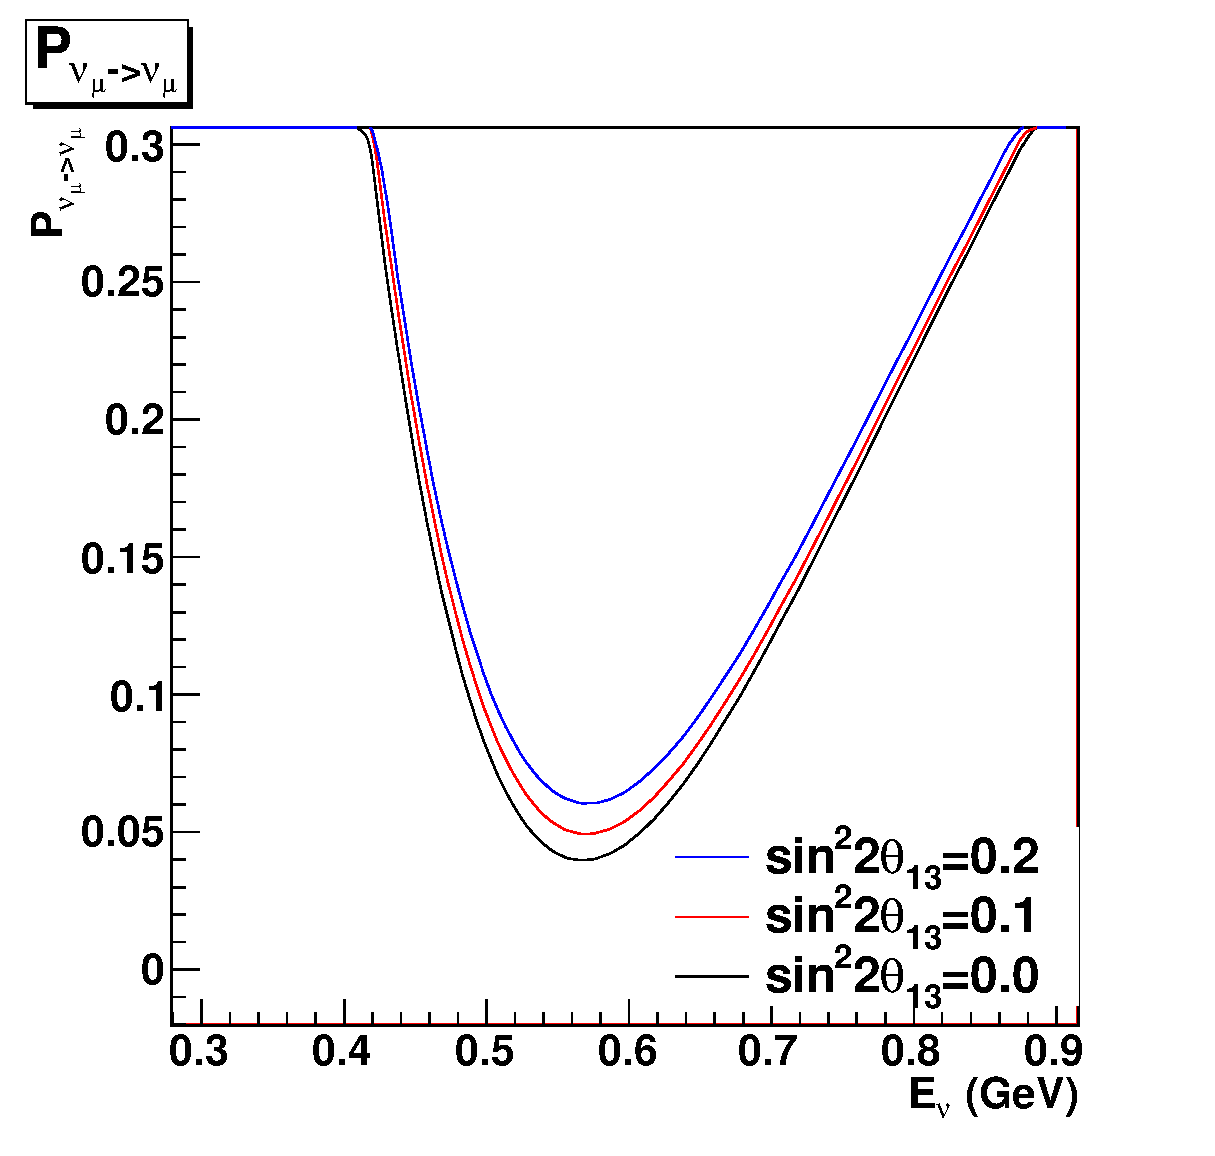
\includegraphics[width=0.45\textwidth]{images/motivation/OscProbNuMuNuMuZoom.eps}
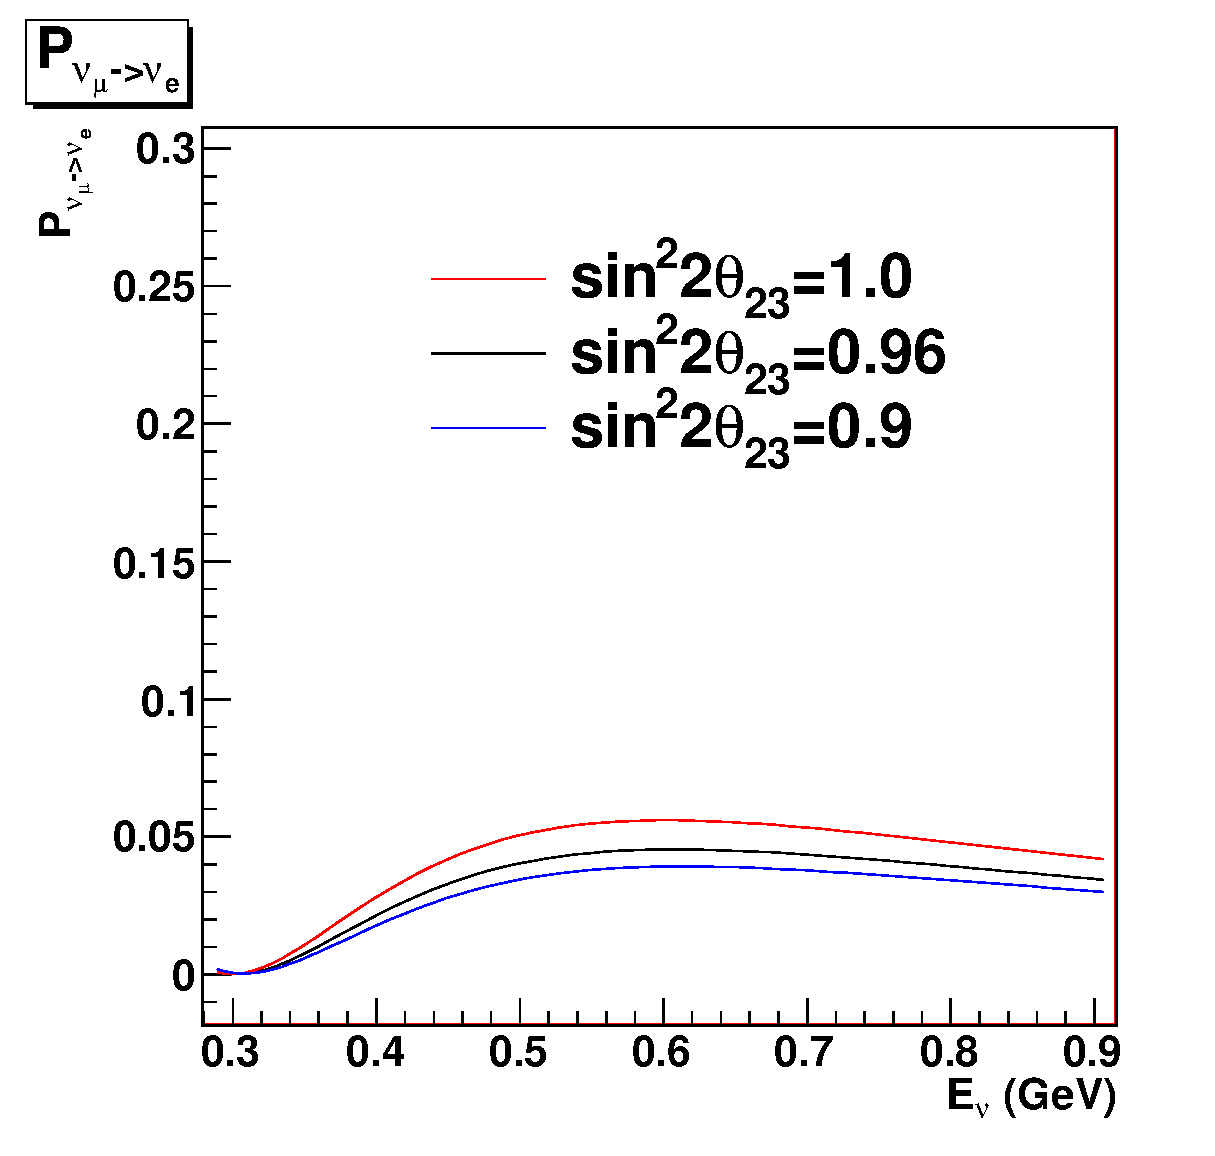
\includegraphics[width=0.45\textwidth]{images/motivation/OscProbNuMuNuEZoom.eps}
\caption{Examples of the effect of the interdependence between the oscillation parameters in the oscillation probabilities $P(\nu_{\mu}\rightarrow\nu_{\mu})$(left) 
and $P(\nu_{\mu}\rightarrow\nu_{e})$ (right). These probabilities are computed for different values of $\sin^{2}2\theta_{13}$ (left) or $\sin^{2}2\theta_{23}$ (right) 
with the other 3 parameters being fixed at $\sin^{2}2\theta_{23}$ = 0.96, $|\Delta m_{32}^{2}|$ = 2.4$\times$10$^{-3}$ eV$^{2}$/c$^{4}$, $\delta_{CP}$ = 0 (left) or 
$\sin^{2}2\theta_{13}$ = 0.1, $|\Delta m_{32}^{2}|$ = 2.4$\times$10$^{-3}$ eV$^{2}$/c$^{4}$, $\delta_{CP}$ = 0 (right).}
\label{fig:oscprob}
\end{center}
\end{figure}


\begin{figure}[htbp]
\begin{center}
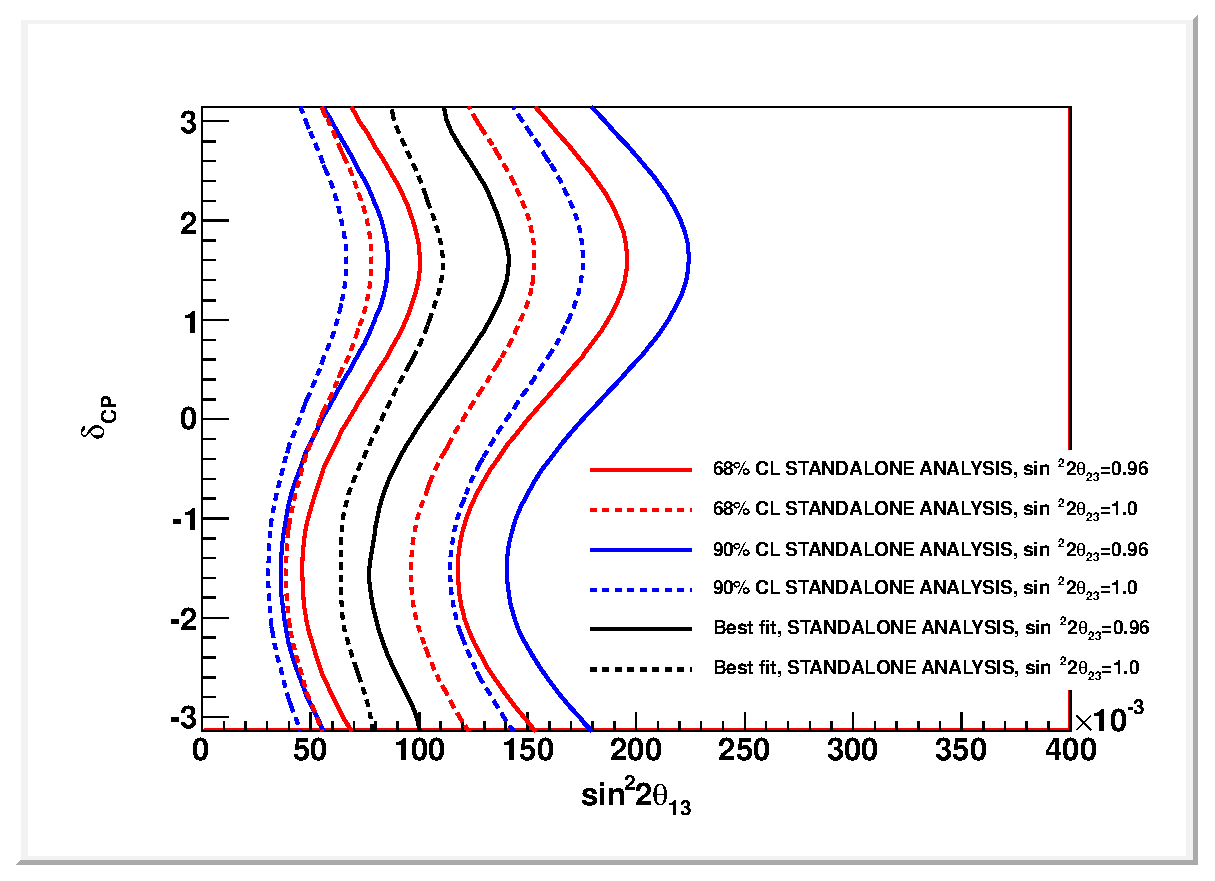
\includegraphics[width=0.7\textwidth]{images/motivation/ComparisonContoursStandaloneDifferentPriors.eps}
\caption{Illustration of the effect of changing the assumed value of $\sin^{2}2\theta_{23}$ in the $\nu_{e}$-appearance contours for 7$\times$10$^{21}$ POT. 
Dashed lines are contours of the stand-alone $\nu_{e}$-appearance analysis assuming maximal mixing ($\sin^{2}2\theta_{23}$ = 1.0), and solid lines are contours 
of the stand-alone $\nu_{e}$-appearance analysis assuming $\sin^{2}2\theta_{23}$ = 0.96, the true value with which the toy experiment was created. The other 
parameters have the following values: $\sin^{2}2\theta_{13}$ = 0.12, $|\Delta m_{32}^{2}|$ = 2.5$\times$10$^{-3}$ eV$^{2}$/c$^{4}$, and $\delta_{CP}$ = 0.5. 
The confidence regions were constructed using the constant-$\Delta\chi^{2}$ method, which is described in Sec.\ \ref{sec:neutrino_oscillation_fitting}.}
\label{fig:effectpriornuecontours}
\end{center}
\end{figure}

 
\begin{figure}[htbp]
\begin{center}
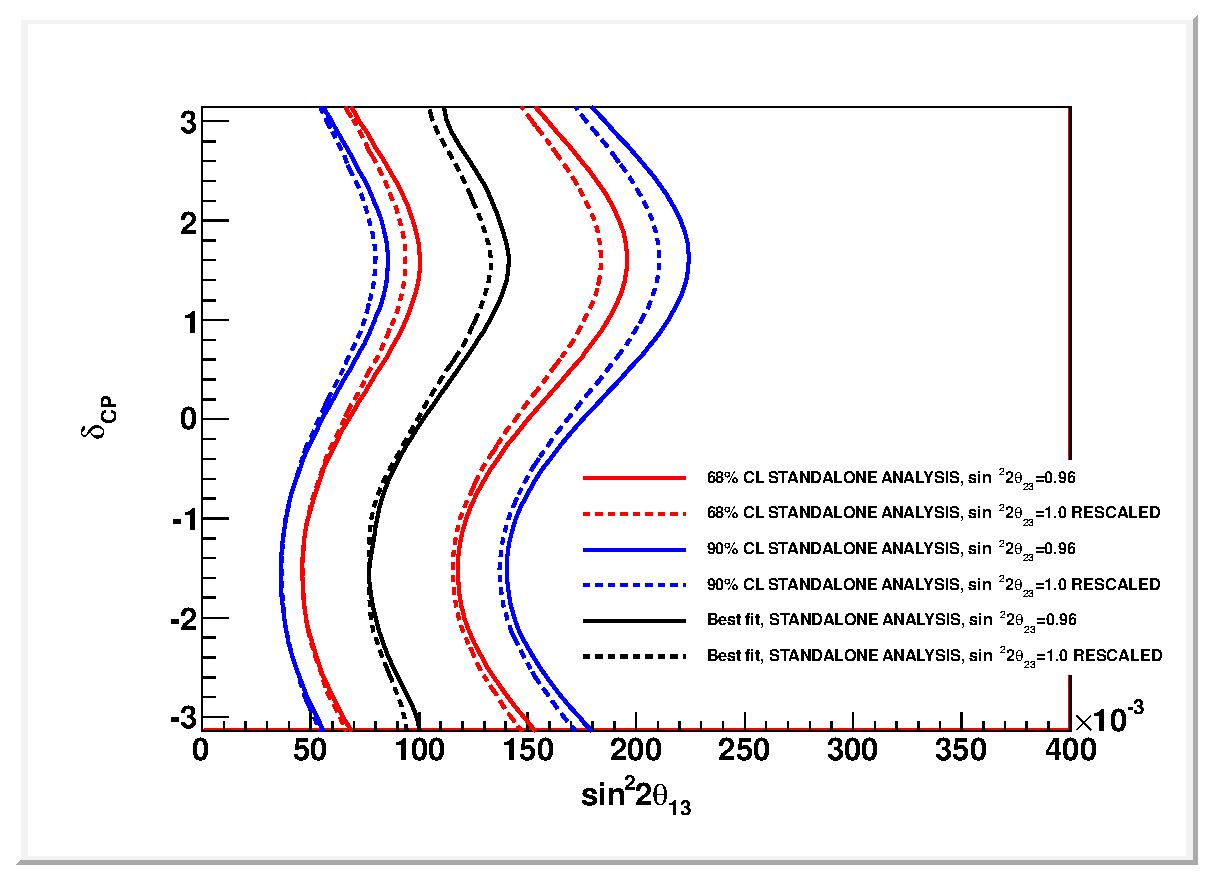
\includegraphics[width=0.7\textwidth]{images/motivation/ComparisonContoursStandaloneDifferentPriorsRescaling.eps}
\caption{Plot of the same contours as in Fig. \ref{fig:effectpriornuecontours} rescaling the contours for maximal prior $\sin^{2}2\theta_{23}$ = 1.0 with the cited 
replacement of $\sin^{2}2\theta_{13}$ by $2 \sin^{2}\theta_{23} \sin^{2}2\theta_{13}$, using for $\theta_{23}$ the true value for the toy experiment.}
\label{fig:comparisoncontoursrescaling}
\end{center}
\end{figure}



\clearpage

\clearpage

\section {Choice of oscillation parameters}
\label{sec:oscparamchoice}

This analysis departs from choices which have been followed historically in the T2K stand-alone $\nu_{e}$-appearance and 
$\nu_{\mu}$-disappearance analyses by changing the oscillation mixing parameters and the mass-squared splitting parameters.
There is a strong motivation for this change in the context of a joint 3-flavour analysis, and it is outlined below.

\subsection* {Neutrino mixing parameters}

In the stand-alone $\nu_{\mu}$-disappearance analysis, $\sin^{2}2\theta_{23}$ is typically measured since it appears in the 
first-order approximate formula for the $\nu_{\mu}$ survival probability:
\begin{equation}
P(\nu_{\mu}\rightarrow\nu_{\mu}) \approx 1 - sin^{2}2\theta_{23} sin^{2} \left(  \frac{\Delta m_{32}^{2} L}{4E_{\nu}}\right)
\end{equation}
In the stand-alone analysis, it is nearly impossible to distinguish $\theta_{23}$ from $\pi/2 - \theta_{23}$, 
as both inputs give the same value for $\sin^{2}2\theta_{23}$ and, therefore, the same $\nu_{\mu}$-survival probability 
This is the so-called octant ambiguity.

\begin{figure}[htbp]
\begin{center}
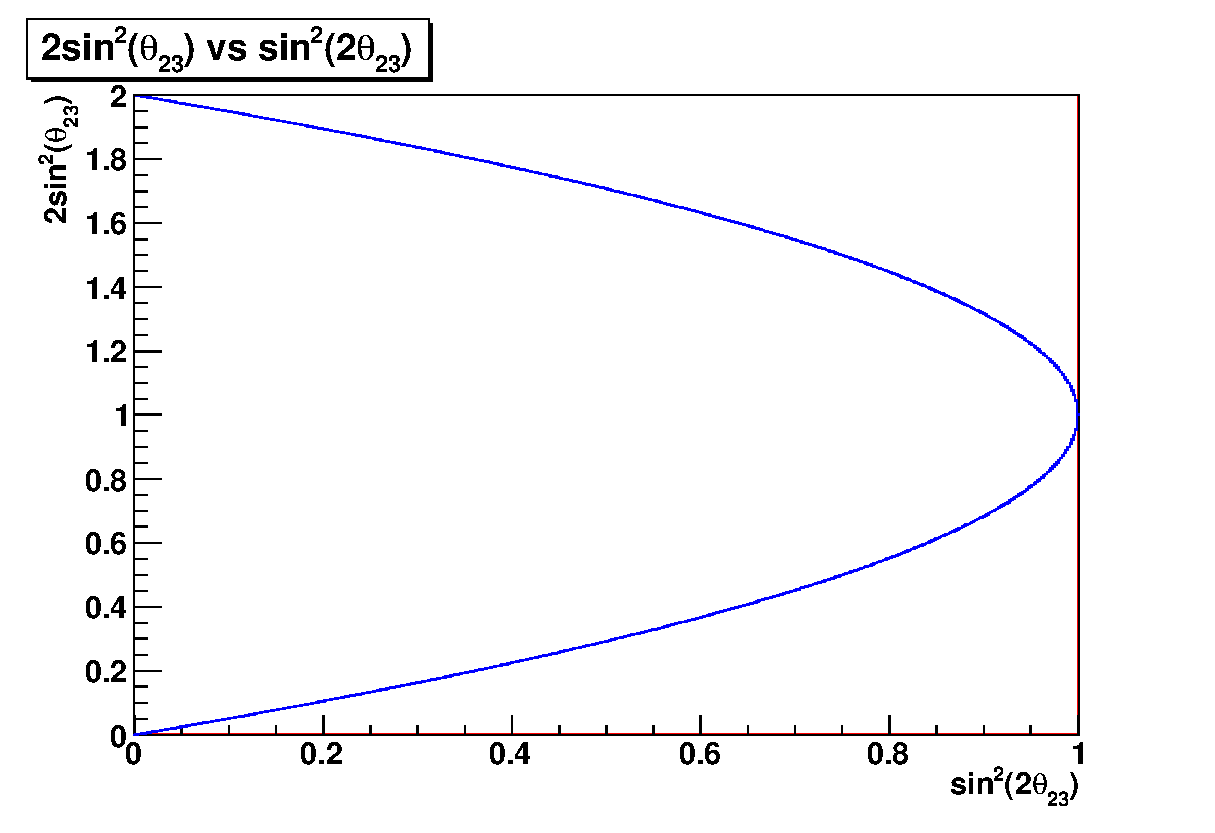
\includegraphics[width=0.5\textwidth]{images/description/Sin2thetaVsSin22theta.eps}
\caption{$\sin^{2}\theta_{23}$ (appears in leading-order term of P($\nu_{\mu}\rightarrow\nu_{e}$) vs $\sin^{2}2\theta_{23}$(
appears in leading-order term of P($\nu_{\mu}\rightarrow\nu_{\mu}$).}
\label{fig:ambig}
\end{center}
\end{figure}
Looking at the leading-order approximation of $P(\nu_{\mu}\rightarrow\nu_{e})$, the 23-sector mixing parameter appears as $\sin^{2}\theta_{23}$:
\begin{equation}
P(\nu_{\mu}\rightarrow\nu_{e}) \approx sin^{2}2\theta_{13}sin^{2}\theta_{23} sin^{2} \left(  \frac{\Delta m_{31}^{2} L}{4E_{\nu}}\right)
\end{equation}

\noindent
it is possible to lift the octant degeneracy by combining the $\nu_{\mu}$-disappearance and $\nu_{e}$-appearance analyses, as shown 
graphically in Fig.\ \ref{fig:ambig}. It is therefore a more natural choice for the joint 3-flavour oscillation analysis to fit for 
$\sin^{2}\theta_{ij}$ rather than $\sin^{2}2\theta_{ij}$, and this is the choice that has been implemented in the VALOR analysis framework.
The option to fit for $\sin^{2}2\theta_{ij}$ has also been retained for backward compatibility and to allow validation checks.

%
%variables in global fits performed by theorists \cite{LisiGlobalAnalysis}, \cite{ConchaMaltoniGlobalAnalysis}, 
%and was already suggested in the collaboration by Mauro Mezzetto and others. 
%Some experiments in the past already used variables in $sin^{2}\theta$ (or $tan^{2}\theta$) 
%such as KamLAND \cite{KamLAND2008Paper}. 
%This choice of the mixing angles will make possible the study of the octant degeneracy of the 
%parameter $\theta_{23}$ as it has been introduced in this note and discussed in 
%several presentations for analysis meetings; however the analysis for the octant 
%degeneracy is going to be described in the documentation for next 2012 joint oscillation analysis. 
%

% Mass square splitting parameters
\subsection* {Mass-squared splitting parameters}
\label{sec:masschoice}

Previous T2K analyses have used the following mass-squared splitting parameters:
\begin{center}
$\left( |\Delta m_{32}^{2}|, \Delta m_{21}^{2} \right)$ 
\end{center}
which are defined as $\Delta m_{ij}^{2} = m_{i}^{2} - m_{j}^{2}$ according to the PDG notation \cite{PDG}. 
The mass hierarchy is set through the sign of $\Delta m_{32}^{2}$
i.e.\ $\Delta m_{32}^{2} = |\Delta m_{32}^{2}|$ in the normal hierarchy 
and $\Delta m_{32}^{2} = - |\Delta m_{32}^{2}|$ in the inverted hierarchy. 
The remaining mass-squared splitting is defined as $\Delta m_{31}^{2} = \Delta m_{32}^{2} + \Delta m_{21}^{2}$ for both hierarchies.

In the normal hierarchy (NH) $m_{1}^{2}<m_{2}^{2}<<m_{3}^{2}$, while in the inverted hierarchy (IH) $m_{3}^{2}<<m_{1}^{2}<m_{2}^{2}$,
i.e.\ $|\Delta m_{31}^{2}|$ is the largest mass-squared splitting in the NH, whereas $|\Delta m_{32}^{2}|$ is the largest in the IH. 
This means that it is not possible to compare the two hierarchies if the atmospheric mass-squared difference is input as 
$|\Delta m_{32}^{2}|$. This has been pointed out by several authors and different schemes are typically employed in global
oscillation fits to circumvent this issue. The VaLOR joint oscillation analysis uses the scheme defined by Fogli and Lisi in 
\cite{LisiGlobalAnalysis} \cite{Fogli} in which $\left( |\Delta m_{32}^{2}|, \Delta m_{21}^{2} \right)$ are replaced by:
\begin{center}
$\left( |\Delta m^{2}|, \delta m^{2} \right)$
\end{center}
where 
$\Delta m^{2} = \left(m_{3}^{2} - \frac {m_{1}^{2}+m_{2}^{2}} {2} \right) =  \left( \frac {\Delta m_{31}^{2} + \Delta m_{32}^{2}} {2} \right)$
and 
$\delta m^{2} = \Delta m_{21}^{2}$.
$|\Delta m^{2}|$ is the "atmospheric" squared-mass splitting, which has the same absolute value for both mass hierarchies.
$\delta m^{2}$ is the "solar" squared-mass splitting which is known to be positive. When the mass-squared splittings are input as 
$\left(\Delta m^{2}, \delta m^{2} \right)$, the mass hierarchy is set through the sign of $|\Delta m^{2}|$, and $\Delta m_{32}^{2}$ 
and $\Delta m_{31}^{2}$ are calculated as 
\begin{displaymath}
\begin{split}
\Delta m_{32}^{2} &= \Delta m^{2} - \frac{\delta m^{2}}{2}  \\
\Delta m_{31}^{2} &= \Delta m^{2} + \frac{\delta m^{2}}{2}
\end{split}
\end{displaymath}
for both mass hierarchies. The ability to input the mass-squared differences as $\left( |\Delta m_{32}^{2}|, \Delta m_{21}^{2} \right)$ has also been retained for 
backward compatibility and to allow various validation checks.

The effects of changing the convention for the inputs of the mass-squared splitting parameters on P($\nu_{\mu}\rightarrow\nu_{\mu}$) 
and P($\nu_{\mu}\rightarrow\nu_{e}$) are shown in Fig.\ \ref{fig:oscprobmassdef}. 

\begin{figure}[htbp]
\begin{center}
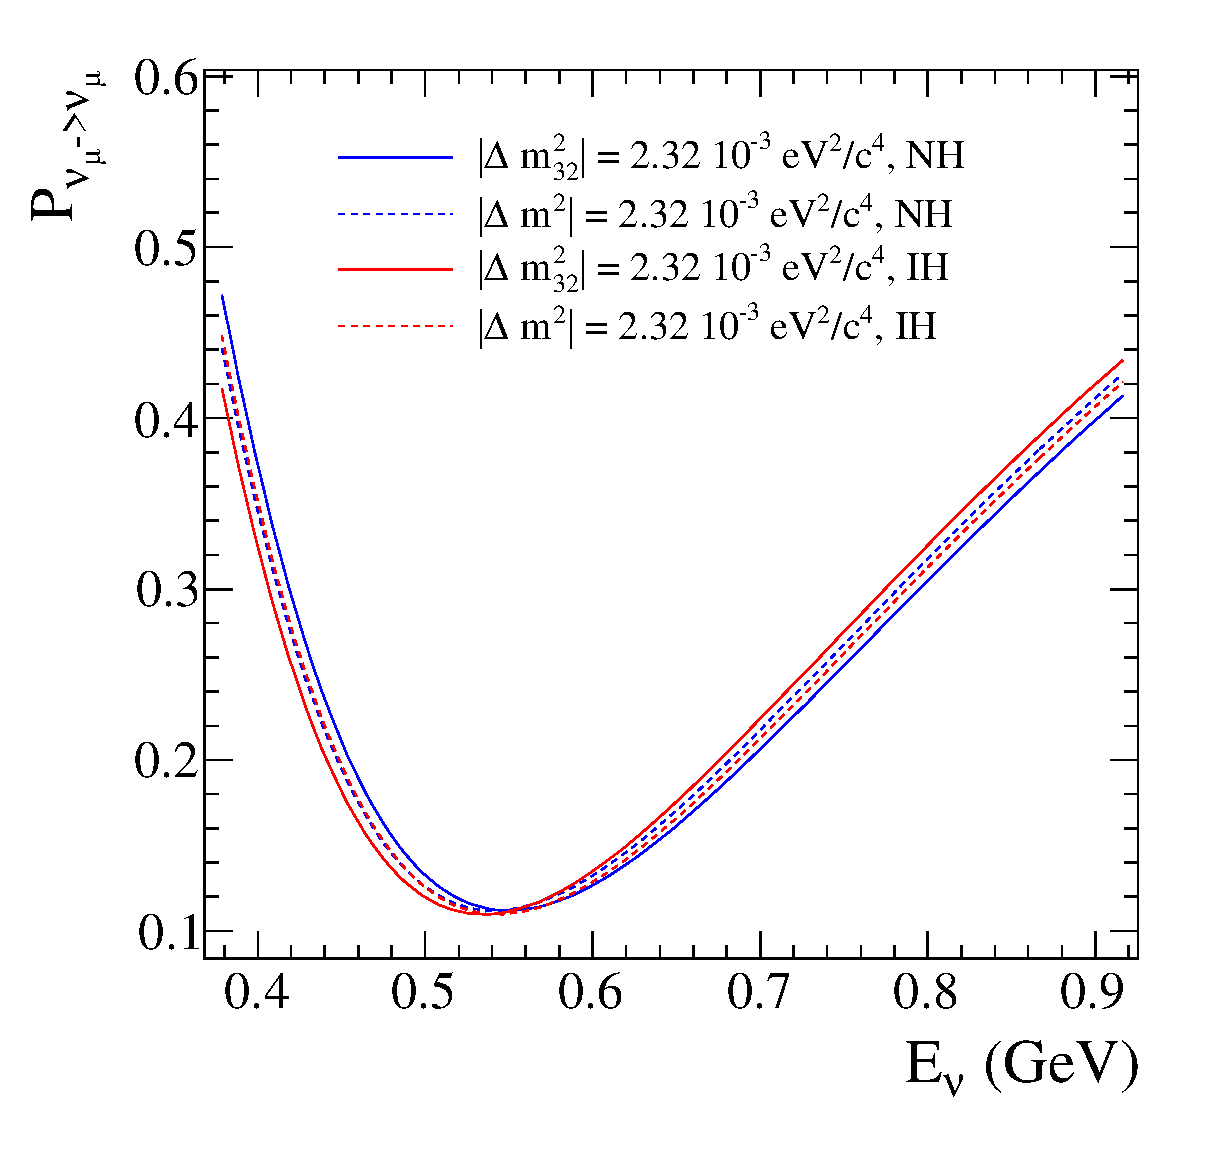
\includegraphics[width=0.5\textwidth]{images/description/OscProbNuMuNuMuMassDef.eps}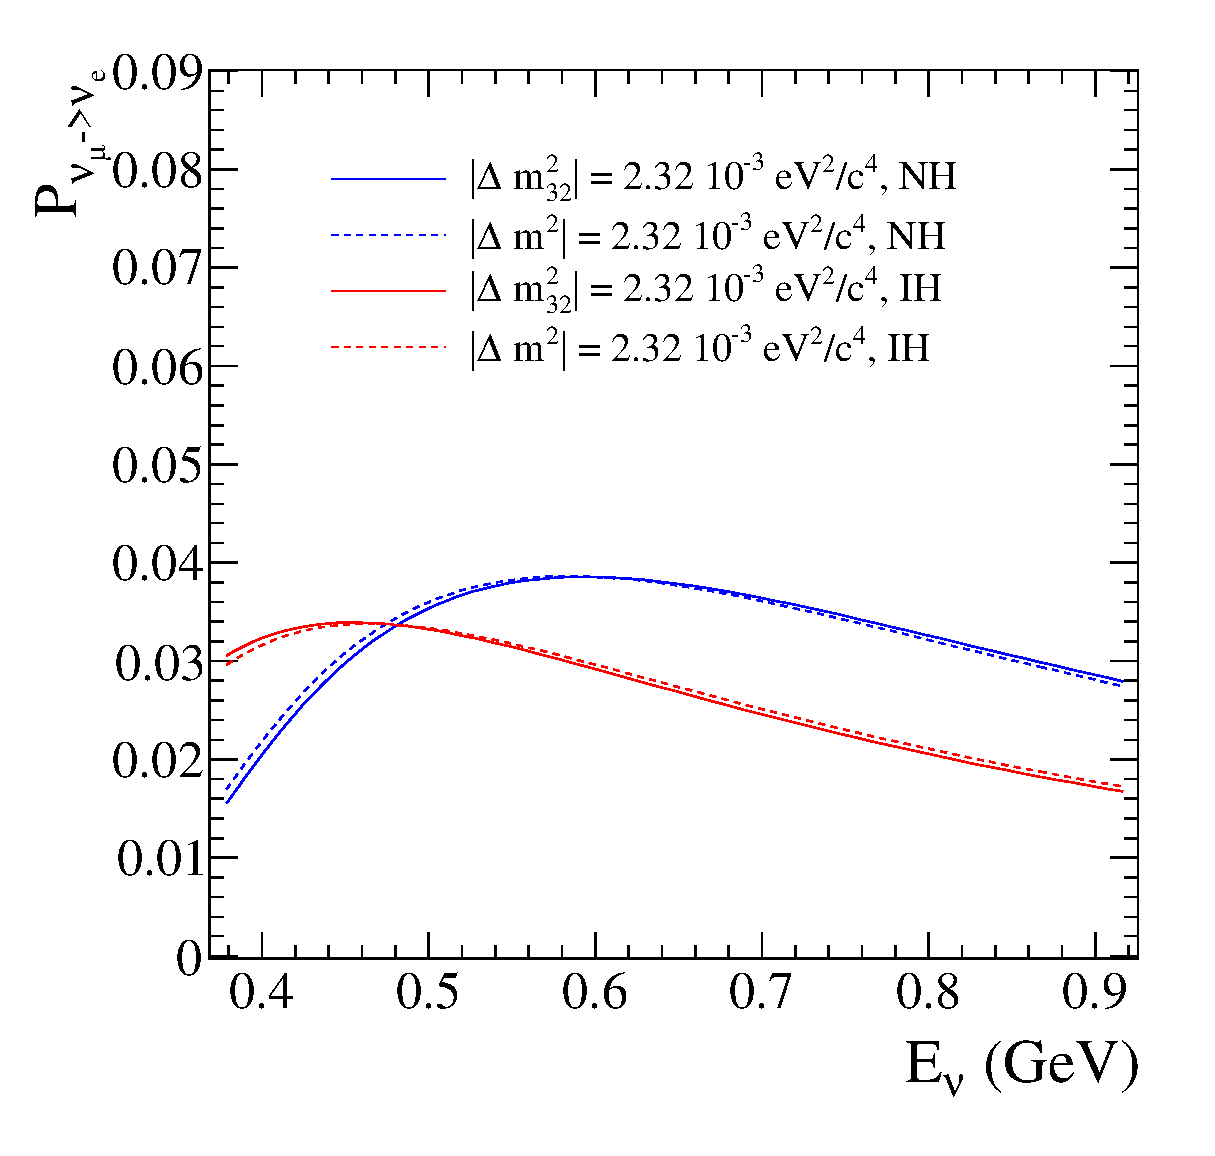
\includegraphics[width=0.5\textwidth]{images/description/OscProbNuMuNuEMassDef.eps}
\caption{
Effects of changing the convention for the inputs of the mass-squared splitting parameters on P($\nu_{\mu}\rightarrow\nu_{\mu}$) (left) and 
P($\nu_{\mu}\rightarrow\nu_{e}$) (right): $|\Delta m_{32}^{2}|$ = 2.32$\times$10$^{-3}$ eV$^{2}$/c$^{4}$ (solid lines) and $|\Delta m^{2}|$ 
= 2.32$\times$10$^{-3}$ eV$^{2}$/c$^{4}$ (dashed lines) for the normal hierarchy (blue) and inverted hierarchy (red). 
 The other oscillation parameters are $\sin^{2}2\theta_{12}$ = 0.857, $\delta m^{2}$ = 7.5$\times$10$^{-5}$ eV$^{2}$/c$^{4}$, 
 $\sin^{2}2\theta_{13}$ = 0.098 (2012 PDG values), $\delta_{CP}$ = 0 and $\sin^{2}2\theta_{23}$ = 0.9. 
}
\label{fig:oscprobmassdef}
\end{center}
\end{figure}

Section \ref{app:fogliandlisi} illustrates the difference in the comparison between results in the two mass hierarchies when using
the Fogli and Lisi convention $\left( |\Delta m^{2}|, \delta m^{2} \right)$ and the previous convention $\left( |\Delta m_{32}^{2}|, \Delta m_{21}^{2} \right)$. 


%Table \ref{tab:numeventsmassdef} shows the predicted number of events of the $1R_{e}$-like events and $1R_{\mu}$-like events using the values from 
%PDG2012 for the oscillation parameters, $sin^{2}2\theta_{12}=0.857, \delta m^{2}=7.50 \times 10^{-5} eV^{2}/c^{4}, sin^{2}2\theta_{13} = 0.098, \delta_{CP}=0$, 
%with $sin^{2}2\theta_{23} =0.9$, changing the mass hierarchy and the mass-squared convention 
%so that either $|\Delta m_{32}^{2}| =2.32 \times 10^{-5} eV^{2}/c^{4}$ or $|\Delta m^{2}| =2.32 \times 10^{-5} eV^{2}/c^{4}$. 
%
%\begin{table}[htbp]
%\begin{tabular} {|p{1cm}|p{1.7cm}|p{1.7cm}|p{1.7cm}|p{1.7cm}||p{1.7cm}|p{1.7cm}|p{1.7cm}|p{1.7cm}|}
%\hline
%  & \multicolumn{4}{|c||} {$1R_{e}$-like events }& \multicolumn{4}{|c|}{ $1R_{\mu}$-like events} \\
% \hline \hline
% &  $|\Delta m_{32}^{2}|$  NH & $|\Delta m^{2}|$ NH & $|\Delta m_{32}^{2}| $ IH & $|\Delta m^{2}| $ IH &  $|\Delta m_{32}^{2}|$ NH & $|\Delta m^{2}|$ NH & $|\Delta m_{32}^{2}|$ IH & $|\Delta m^{2}| $ IH \\
%\hline \hline
%Total  & 10.984 & 10.985 & 9.437 & 9.489 & 60.940 & 61.842 & 62.656 & 61.652 \\
%\hline 
%$\nu_{\mu}$  &  1.213 &  1.214 & 1.216 & 1.214 & 56.860 & 57.730 & 58.530 & 57.560 \\
%\hline
%$\bar{\nu_{\mu}}$  & 0.067 & 0.067 & 0.067 &  0.067 & 3.812 & 3.851 & 3.885 & 3.845 \\
%\hline
%$\nu_{e}$  & 1.509 & 1.510 & 1.526 & 1.525 & 0.135 & 0.135 & 0.135 & 0.135 \\
%\hline
%$\bar{\nu_{e}}$  &  0.079 & 0.079 &  0.079 & 0.078 & 0.013 & 0.013 &  0.013 & 0.013 \\
%\hline
%osc. $\nu_{e}$ & 8.117 & 8.116 & 6.551 & 6.604 & 0.118 &  0.118 & 0.096 & 0.097 \\
%\hline
%\end{tabular}
%\caption{Table of predicted number of events of the $1R_{e}$-like events and $1R_{\mu}$-like events using the values from PDG2012 for the oscillation parameters, $sin^{2}2\theta_{12}=0.857, \delta m^{2}=7.50 \times 10^{-5} eV^{2}/c^{4}, sin^{2}2\theta_{13} = 0.098, \delta_{CP}=0$ , with $sin^{2}2\theta_{23} =0.9$, changing the mass hierarchy and the mass-squared convention so that either $|\Delta m_{32}^{2}| =2.32 \times 10^{-5} eV^{2}/c^{4}$ or $|\Delta m^{2}| =2.32 \times 10^{-5} eV^{2}/c^{4}$}
%\label{tab:numeventsmassdef}
%\end{table}
%


\subsection* {Treatment of solar (12-sector) oscillation parameters}

A study has been made in which $\sin^{2}2\theta_{12}$ and $\Delta m_{21}^{2}$ were allowed to float in the fit of the single $\mu$-like ring Super K sample, and 
the results are shown in Appendix \ref{app:solar}. It was found that the fitter returned extreme values of these parameters (see Fig.\ \ref{fig:solarfit}), and 
this is because they have no effect on the single $\mu$-like ring sample. For this reason, these parameters were fixed throughout this analysis to the values 
in table \ref{tab:solarparameters}.

\begin{table}[h]
\centering
\begin{tabular}{|c|c|}
\hline
Parameter & Value \\
\hline
\hline
$\sin^{2}2\theta_{12}$ & 0.857 \\
\hline 
$\sin^{2}\theta_{12}$ & 0.311 \\
\hline 
$\Delta m_{21}^{2}$ & 7.5$\times$10$^{-5}$ eV$^{2}$/c$^{4}$ \\
\hline
\end{tabular}
\caption{Values used for $\sin^{2}2\theta_{12}$ and $\Delta m_{21}^{2}$ in the joint oscillation analysis}
\label{tab:solarparameters}
\end{table}




%\clearpage

\section{Predictions of single $\mu$-like ring and single e-like ring event reconstructed energy spectrum in SuperK}
\label{sec:prediction}

The predicted number $N_{SK;s,r}$
of events
in the $r^{th}$ reconstructed energy bin
in the SuperK sample $s$ (single $\mu$-like ring or single e-like ring)
is computed as follows:

\begin{equation}
\displaystyle
  N^{exp}_{SK;s,r} =
    \sum_{m} \sum_{t} \sum_{r\prime}
        \color{green}{P_{m,t}} \cdot
        \color{blue}{T_{s,r,r\prime,f_{{\Delta}E},s}} \cdot
        \color{red}{S_{s,m,t,r\prime,\textbf{f}}} \cdot
        \color{orange}{N_{SK;s,m,r\prime,t}^{MC}} 
\label{eq:far_prediction}
\end{equation}

In Eq.\ \ref{eq:far_prediction}, $N_{SK;s,m,r\prime,t}^{MC}$ is the input SuperK Monte Carlo (MC) template
describing the number of events in the sample $s$, with true reaction mode $m$,
that can be found in the true energy bin t and in the reconstructed energy bin $r\prime$.
Notice that $r\prime$ index indicates a SuperK reconstructed energy bin in absence of a shift in
reconstructed energy scale and the index r indicates a SuperK reconstructed energy bin after a shift in the
reconstructed energy scale is applied.
The construction of the nominal MC templates was presented in detail in 
Sec.\ 2.2 of Ref.\ \cite{OurRun123DisappAnalysis3Flavour} 
describing the {\em VaLOR} 2012 Run 1+2+3 $\nu_{\mu}$-disappearance analysis.
The method described there was extended to construct the MC templates relevant for the 
calculation of the predicted single e-like ring event reconstructed energy p.d.f.
The nominal MC templates are reweighted using both
flux-tuning weights based on NA61 hadro-production data (see Sec.\ 2.3 of Ref. \cite{OurRun123DisappAnalysis3Flavour})
and flux and cross-section tuning weights based on ND280 data (see Sec.\ 2.4 of Ref. \cite{OurRun123DisappAnalysis3Flavour}).
For the calculation of the single $\mu$-like ring event reconstructed energy p.d.f.,
the same 28 MC templates are used as in the {\em VaLOR} 2012 Run 1+2+3 $\nu_{\mu}$-disappearance analysis 
(see Sec.\ 2.2.4 in \cite{OurRun123DisappAnalysis3Flavour}).
However 32 MC templates are used for the calculation of the single e-like ring event reconstructed energy p.d.f.
as a different choice was made for the NC MC templates.
For the single $\mu$-like ring p.d.f.
the `NC1$\pi^{\pm}$' and `NC other' MC templates are used, 
whereas for the single e-like ring p.d.f. the `NC1$\pi^{0}$', `NC coherent' and `NC other' templates are used. 
Consequently, the definition of `NC other' is different for the two samples.
In total, 60 MC templates are used for the 
calculation of the combined single $\mu$-like ring and single e-like ring event reconstructed energy p.d.fs.
These templates are listed in Tab.\ \ref{tab:list_of_templates}.
The MC template binning for the single $\mu$-like ring sample is unchanged from the {\em VaLOR} 2012 Run 1+2+3 $\nu_{\mu}$-disappearance analysis\footnote{
  Each MC templates has 6132 2-dimensional bins (= 84 true energy bins $\times$ 73 reconstructed energy bins).
  The 84 true energy bins are arranged as follows:
    6  50-MeV bins from 0-0.3 GeV,
   28  25-MeV bins from 0.3-1 GeV,
   40  50-MeV bins from 1-3 GeV,
    5 100-MeV bin from 3-3.5 GeV,
    1 bin from 3.5-4 GeV,
    1 bin from 4-5 GeV,
    1 bin from 5-7 GeV,
    1 bin from 7-10 GeV and
    1 bin from 10-30 GeV.
The 73 reconstructed energy bins are as follows:
    60   50-MeV bins from 0-3 GeV,
     4  250-MeV bins from 3-4 GeV,
     4  500-MeV bins from 4-6 GeV,
     4 1000-MeV bins from 6-10 GeV and
     1 bin from 10-30 GeV.
}. For the single e-like ring sample the MC templates have the same 84 true energy bins used for the single $\mu$-like ring sample
and 25 reconstructed energy bins from 0 to 1.25 GeV (50 MeV/bin). 

The term $S_{s,m,t,r\prime,\vec{f}}$ in Eq.\ \ref{eq:far_prediction} is an overall, multiplicative, systematic error factor
depending on the sample $s$, the reaction mode $m$, the true energy bin $t$, the reconstructed energy bin $r\prime$
and a vector of nuisance (systematic) parameters $\vec{f}$.
A summary of the nuisance parameters considered in this analysis is given in Sec.\ \ref{sec:systematics} of this note.
$T_{r;r\prime;f_{{\Delta}E}}$ is a transfer function describing the migration of events
between the reconstructed energy bins $r$ and $r\prime$ due to a potential shift in the SuperK reconstructed energy
scale, expressed here in terms of the nuisance parameter $f_{{\Delta}E}$.
Finally, $P_{m;t}$ is the 3-flavour oscillation probability applied in the true energy
bin $t$ of the SuperK MC template which corresponds to mode $m$.
The CC MC templates constructed from the unoscillated MC samples are weighted
with the corresponding survival probability:
The $\nu_{\mu}$ CC templates are weighted with P($\nu_{\mu}\rightarrow\nu_{\mu}$),
the $\bar{\nu}_{\mu}$ CC templates with P($\bar{\nu}_{\mu}\rightarrow\bar{\nu}_{\mu}$),
the $\nu_{e}$ CC templates with P($\nu_{e}\rightarrow\nu_{e}$) and
the $\bar{\nu}_{e}$ CC templates with P($\bar{\nu}_{e}\rightarrow\bar{\nu}_{e}$).
The CC MC templates made from the oscillated $\nu_{e}$ MC sample are weighted with
P($\nu_{\mu}\rightarrow\nu_{e}$) (the sample was generated assuming 100\% of
$\nu_{\mu}$ oscillate to $\nu_{e}$).
Contributions from $\nu_{\tau}$-CC and $\bar{\nu}_{\tau}$-CC are neglected, as their
energy threshold is around 3.5 GeV and their effect is negligible.
The same oscillation parameters
are used for both $\nu_{\mu}$ and $\bar{\nu}_{\mu}$ oscillations.
Oscillations are not applied to the NC MC templates
since they serve as proxies for the mixtures of
$\nu_{e}+\nu_{\mu}+\nu_{\tau}$ NC and
$\bar{\nu}_{e}+\bar{\nu}_{\mu}+\bar{\nu}_{\tau}$ NC MC templates
which are unchanged under 3-flavour oscillations.
All oscillation probabilities are computed in a 3-flavour framework including matter effects in constant-density matter
(assuming an Earth crust density of 2.6 g/cm$^{3}$).
Custom oscillation probability calculation code was developed within the {\em VaLOR} analysis framework.
Details and estimates of the numerical accuracy of this code can be found in 
Appendices A and B of Ref. \cite{OurRun123DisappAnalysis3Flavour}.

Fig.\ \ref{fig:Nsk1Rmu_vs_Dmsq_theta23_tunedmc} (Fig.\ \ref{fig:Nsk1Re_vs_dcp_theta13_tunedmc}) 
shows the predicted number of single  $\mu$-like ring (single e-like ring) events 
as a function of $\sin^{2}\theta_{23}$ and $|\Delta m^{2}|$ ($\sin^{2}\theta_{13}$ and $\delta_{CP}$), that is,   
the only two oscillations parameters allowed to float by the stand-alone 
$\nu_{\mu}$-disappearance ($\nu_{e}$-appearance) analysis.
In Fig.\ \ref{fig:Nsk1Rmu_vs_dcp_theta13_tunedmc} (Fig.\ \ref{fig:Nsk1Re_vs_Dmsq_theta23_tunedmc}),
the predicted number of single $\mu$-like ring (single e-like ring) events
is shown as function of $\sin^{2}\theta_{13}$ and $\delta_{CP}$ ($\sin^{2}\theta_{23}$ and $|\Delta m^{2}|$).
This dependency has been ignored by the stand-alone $\nu_{\mu}$-disappearance ($\nu_{e}$-appearance) analysis 
to date, but it is taken into account in the joint 3-flavour oscillation analysis.

Typical single $\mu$-like ring (single e-like ring) event reconstructed energy spectra,
and spectral components, are shown in 
Fig.\ \ref{fig:1Rmu_spectrum_and_components_no_osc} (Fig.\ \ref{fig:1Re_spectrum_and_components_no_osc})
for no oscillations and in 
Fig.\ \ref{fig:1Rmu_spectrum_and_components_default_osc} (Fig.\ \ref{fig:1Re_spectrum_and_components_default_osc})
for oscillations with typical parameters (see caption).
All these plots are generated for an exposure of 3.010$\times$10$^{20}$ POT
and using the BANFF-tuned MC templates.

Finally, the calculated numbers of single $\mu$-like ring and single e-like ring events using the nominal MC templates,
the NA61-tuned MC templates and the BANFF-tuned MC templates are shown in Tab.\ \ref{tab:nsk_nominal_x3_no_osc} for no oscillations
and in Tab.\ \ref{tab:nsk_nominal_x3_default_osc} for oscillations with typical parameters (see caption).
The total numbers of events and the numbers of events from each mode considered in this analysis are shown.
These numbers were calculated for an exposure of 3.010$\times$10$^{20}$ POT.


%...........
%
% list of templates
%
\begin{table}
\centering
\begin{tabular}{| c | c | c | }
\hline  
          & single $\mu$-like ring sample &  single e-like ring sample \\
\hline  
$\nu_\mu$ CCQE &                                                                    \ck      &     \ck         \\
$\nu_\mu$ CC 1$\pi$ &                                                               \ck      &     \ck         \\
$\nu_\mu$ CC coherent &                                                             \ck      &     \ck         \\
$\nu_\mu$ CC other &                                                                \ck      &     \ck         \\
$\nu_\mu$/$\nu_\tau$ NC 1$\pi^{+/-}$ &                                              \ck      &                 \\
$\nu_\mu$/$\nu_\tau$ NC 1$\pi^{0}$ &                                                         &     \ck         \\
$\nu_\mu$/$\nu_\tau$ NC coherent &                                                           &     \ck         \\
$\nu_\mu$/$\nu_\tau$ NC other &                                                     \ck      &     \ck         \\
$\bar{\nu}_{\mu}$ CCQE &                                                            \ck      &     \ck         \\
$\bar{\nu}_{\mu}$ CC 1$\pi$ &                                                       \ck      &     \ck         \\
$\bar{\nu}_{\mu}$ CC coherent &                                                     \ck      &     \ck         \\
$\bar{\nu}_{\mu}$ CC other &                                                        \ck      &     \ck         \\
$\bar{\nu}_{\mu}$/$\bar{\nu}_{\tau}$ NC 1$\pi^{+/-}$ &                              \ck      &                 \\
$\nu_\mu$/$\nu_\tau$ NC 1$\pi^{0}$ &                                                         &     \ck         \\
$\nu_\mu$/$\nu_\tau$ NC coherent &                                                           &     \ck         \\
$\bar{\nu}_{\mu}$/$\bar{\nu}_{\tau}$ NC other &                                     \ck      &     \ck         \\
$\nu_e$ CCQE &                                                                      \ck      &     \ck         \\
$\nu_e$ CC 1$\pi$ &                                                                 \ck      &     \ck         \\
$\nu_e$ CC coherent &                                                               \ck      &     \ck         \\
$\nu_e$ CC other &                                                                  \ck      &     \ck         \\
$\nu_e$ NC 1$\pi^{+/-}$ &                                                           \ck      &                 \\
$\nu_\mu$/$\nu_\tau$ NC 1$\pi^{0}$ &                                                         &     \ck         \\
$\nu_\mu$/$\nu_\tau$ NC coherent &                                                           &     \ck         \\
$\bar{\nu}_{\mu}$/$\bar{\nu}_{\tau}$ NC other &                                     \ck      &     \ck         \\
$\nu_e$ CCQE &                                                                      \ck      &     \ck         \\
$\nu_e$ CC 1$\pi$ &                                                                 \ck      &     \ck         \\
$\nu_e$ CC coherent &                                                               \ck      &     \ck         \\
$\nu_e$ CC other &                                                                  \ck      &     \ck         \\
$\nu_e$ NC 1$\pi^{+/-}$ &                                                           \ck      &                 \\
$\nu_\mu$/$\nu_\tau$ NC 1$\pi^{0}$ &                                                         &     \ck         \\
$\nu_\mu$/$\nu_\tau$ NC coherent &                                                           &     \ck         \\
$\nu_e$ NC other &                                                                  \ck      &     \ck         \\
$\bar{\nu}_{e}$ CCQE &                                                              \ck      &     \ck         \\
$\bar{\nu}_{e}$ CC 1$\pi$ &                                                         \ck      &     \ck         \\
$\bar{\nu}_{e}$ CC coherent &                                                       \ck      &     \ck         \\
$\bar{\nu}_{e}$ CC other &                                                          \ck      &     \ck         \\
$\bar{\nu}_{e}$ NC 1$\pi^{+/-}$  &                                                  \ck      &                 \\
$\nu_\mu$/$\nu_\tau$ NC 1$\pi^{0}$ &                                                         &     \ck         \\
$\nu_\mu$/$\nu_\tau$ NC coherent &                                                           &     \ck         \\
$\bar{\nu}_{e}$ NC other &                                                          \ck      &     \ck         \\
Osc. $\nu_e$ CCQE &                                                                 \ck      &     \ck         \\
Osc. $\nu_e$ CC 1$\pi$ &                                                            \ck      &     \ck         \\
Osc. $\nu_e$ CC coherent &                                                          \ck      &     \ck         \\
Osc. $\nu_e$ CC other &                                                             \ck      &     \ck         \\
\hline
\end{tabular}
\caption{
  List of the MC templates used for the calculation of the {\em VaLOR}
  single $\mu$-like ring and single e-like ring 
  event reconstructed energy spectrun p.d.f.s.
  The symbol \ck indicates, in any row, for which of the samples defined in the last two columns
  the MC template defined in the first column is used.
  Notice that the MC templates used for NC modes are different for
  single $\mu$-like ring and single e-like ring. 
}
\label{tab:list_of_templates}
\end{table}



%...........
%
% NSK 1Rmu, 1Re vs osc params
%
\begin{figure*}[htb]
\begin{minipage}[t]{0.48\linewidth}
\center
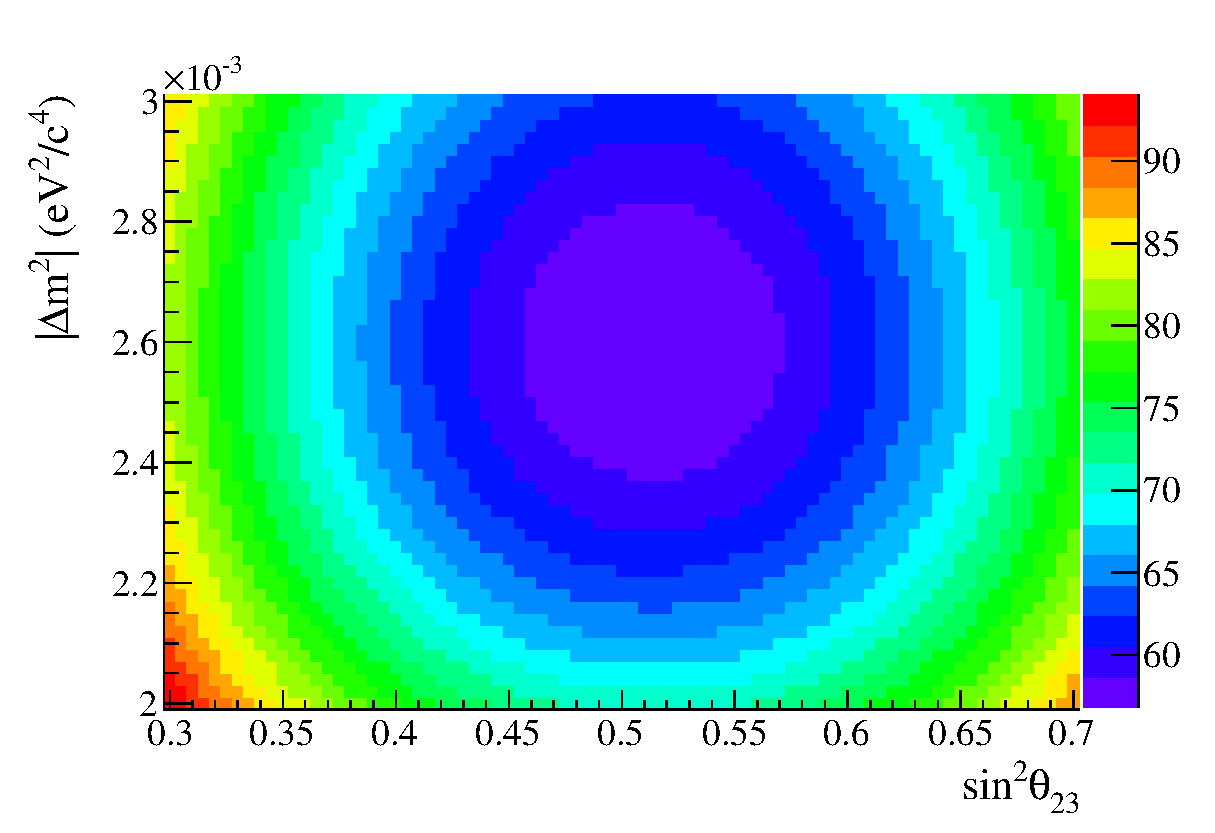
\includegraphics[width=20pc]{./images/prediction/Nsk_1Rmu_disap.eps}
\caption {
  Predicted number of single $\mu$-like ring events,
  as a function of $\sin^{2}\theta_{23}$ and $|\Delta m^{2}|$,
  for an exposure of 3.010$\times$10$^{20}$ POT.
  The number of events was calculated using the BANFF-tuned MC templates.
  2012 PDG values are used for $\sin^{2}\theta_{13}$, $\sin^{2}\theta_{12}$ and $\delta m^{2}$ and $\delta_{CP}$=0.
  The numbers shown were generated assuming the normal hierarchy.
}
\label{fig:Nsk1Rmu_vs_Dmsq_theta23_tunedmc}
\end{minipage}
\hspace{0.06\linewidth}
\begin{minipage}[t]{0.48\linewidth}
\center
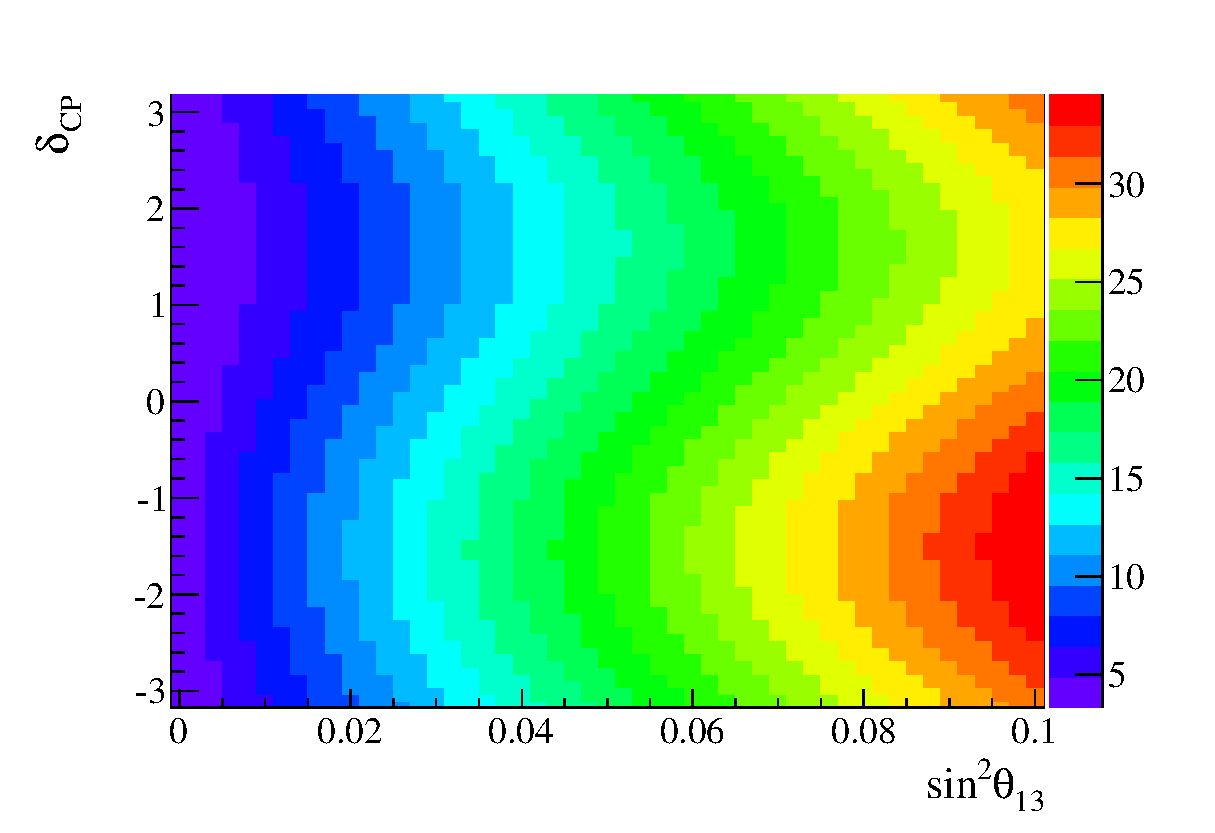
\includegraphics[width=20pc]{./images/prediction/Nsk_1Re_app.eps}
\caption {
  Predicted number of single e-like ring events,
  as a function of $\sin^{2}\theta_{13}$ and $\delta_{CP}$,
  for an exposure of 3.010$\times$10$^{20}$ POT.
  The number of events was calculated using the BANFF-tuned MC templates.
  2012 PDG values are used for $\sin^{2}\theta_{12}$, $|\Delta m^{2}|$ and $\delta m^{2}$,
  while $\sin^{2}\theta_{23}$ was set to 0.5.
  The numbers shown were generated assuming the normal hierarchy.
}
\label{fig:Nsk1Re_vs_dcp_theta13_tunedmc}
\end{minipage}
\end{figure*}


%...........
%
% NSK 1Rmu, 1Re vs osc params typically fixed in stand-alone analyses
%
\begin{figure*}[htb]
\begin{minipage}[t]{0.48\linewidth}
\center
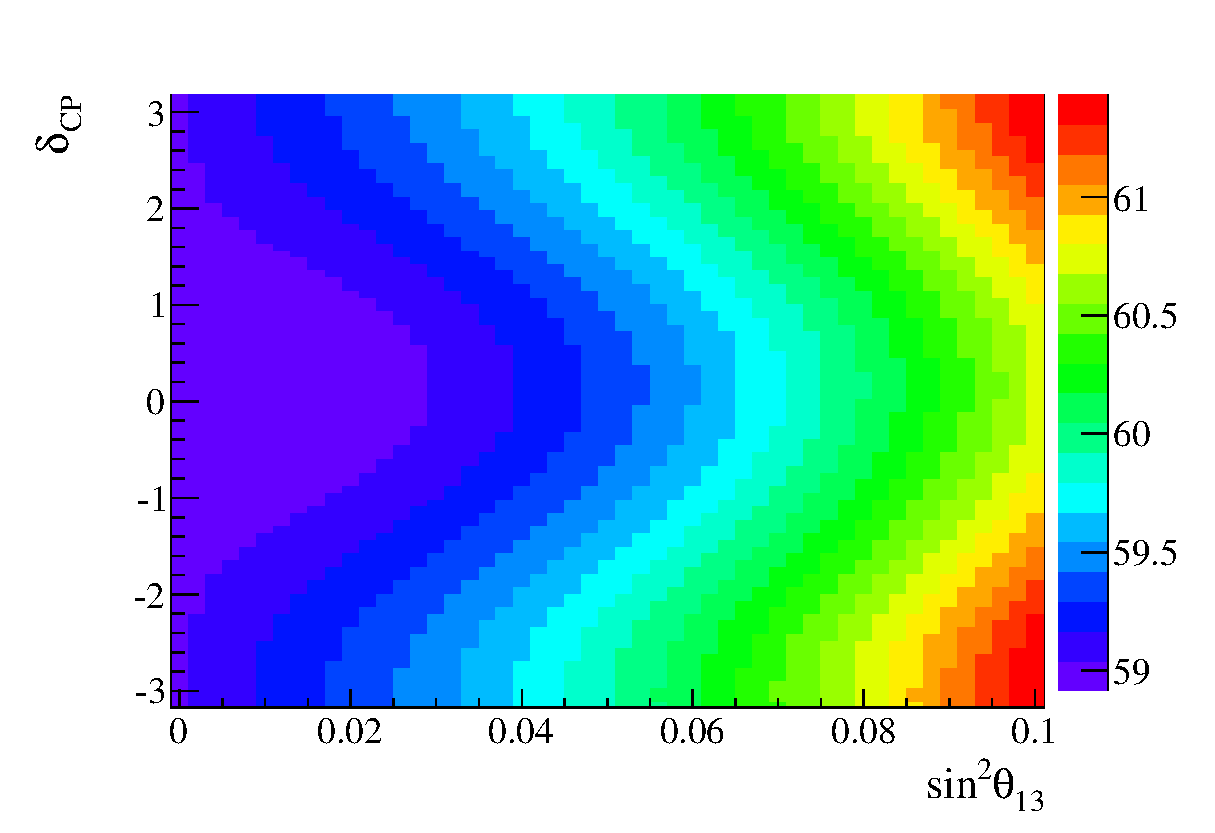
\includegraphics[width=20pc]{./images/prediction/Nsk_1Rmu_app.eps}
\caption {
  Predicted number of single $\mu$-like ring events,
  as a function of $\sin^{2}\theta_{13}$ and $\delta_{CP}$,
  which are typically fixed to constant values by the stand-alone $\nu_{\mu}$-disappearance analysis,
  for an exposure of 3.010$\times$10$^{20}$ POT.
  The number of events was calculated using the BANFF-tuned MC templates.
  2012 PDG values are used for $\sin^{2}\theta_{12}$, $|\Delta m^{2}|$ and $\delta m^{2}$,
  while $\sin^{2}\theta_{23}$ was set to 0.5.
  The numbers shown were generated assuming the normal hierarchy.
}
\label{fig:Nsk1Rmu_vs_dcp_theta13_tunedmc}
\end{minipage}
\hspace{0.06\linewidth}
\begin{minipage}[t]{0.48\linewidth}
\center
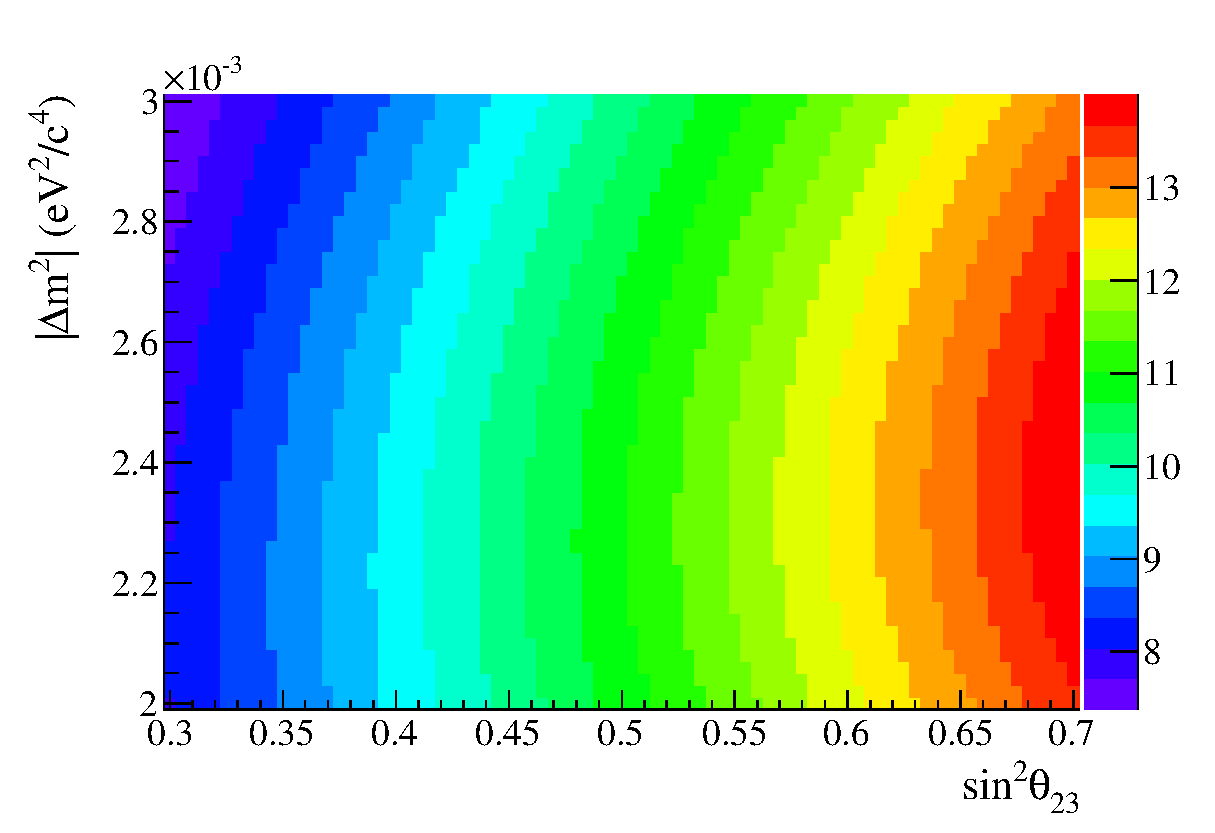
\includegraphics[width=20pc]{./images/prediction/Nsk_1Re_disap.eps}
\caption {
  Predicted number of single e-like ring events,
  as a function of $\sin^{2}\theta_{23}$ and $|\Delta m^{2}|$,
  which are typically fixed to constant values by the stand-alone $\nu_{e}$-appearance analysis,
  for an exposure of 3.010$\times$10$^{20}$ POT.
  The number of events was calculated using the BANFF-tuned MC templates.
  2012 PDG values are used for $\sin^{2}\theta_{13}$, $\sin^{2}\theta_{12}$ and $\delta m^{2}$ and $\delta_{CP}$=0.
  The numbers shown were generated assuming the normal hierarchy.
}
\label{fig:Nsk1Re_vs_Dmsq_theta23_tunedmc}
\end{minipage}
\end{figure*}

%...........
%
% 1Rmu, 1Re spectra - no oscillations
%
\begin{figure*}[htb]
\begin{minipage}[t]{0.48\linewidth}
\center
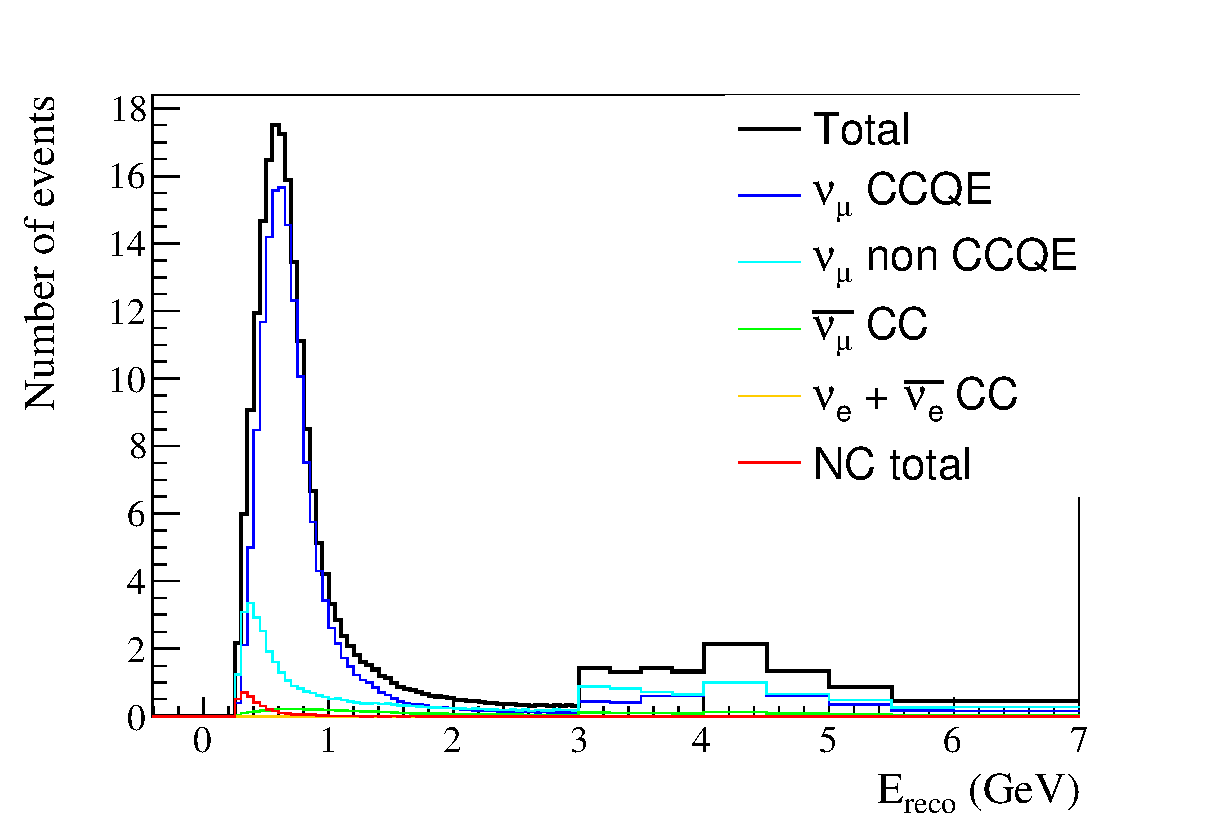
\includegraphics[width=20pc]{./images/prediction/1Rmu_spectrum_no_osc.eps}
\caption {
 Predicted reconstructed-energy spectrum of single $\mu$-like ring events,
 and contributions from various true neutrino reaction modes,
 for no oscillations and
 for an exposure of 3.010$\times$10$^{20}$ POT.
 The 28 components of the spectrum are calculated separately in the actual analysis,
 but, for this plot, are grouped into just 5 categories:
 $\nu_{\mu}$ CCQE, $\nu_{\mu}$ CCnonQE, $\bar{\nu}_{\mu}$ CC, $\nu_{e}$/$\bar{\nu}_{e}$ CC and NC.
 The spectrum was generated using the BANFF-tuned MC templates.
}
\label{fig:1Rmu_spectrum_and_components_no_osc}
\end{minipage}
\hspace{0.06\linewidth}
\begin{minipage}[t]{0.48\linewidth}
\center
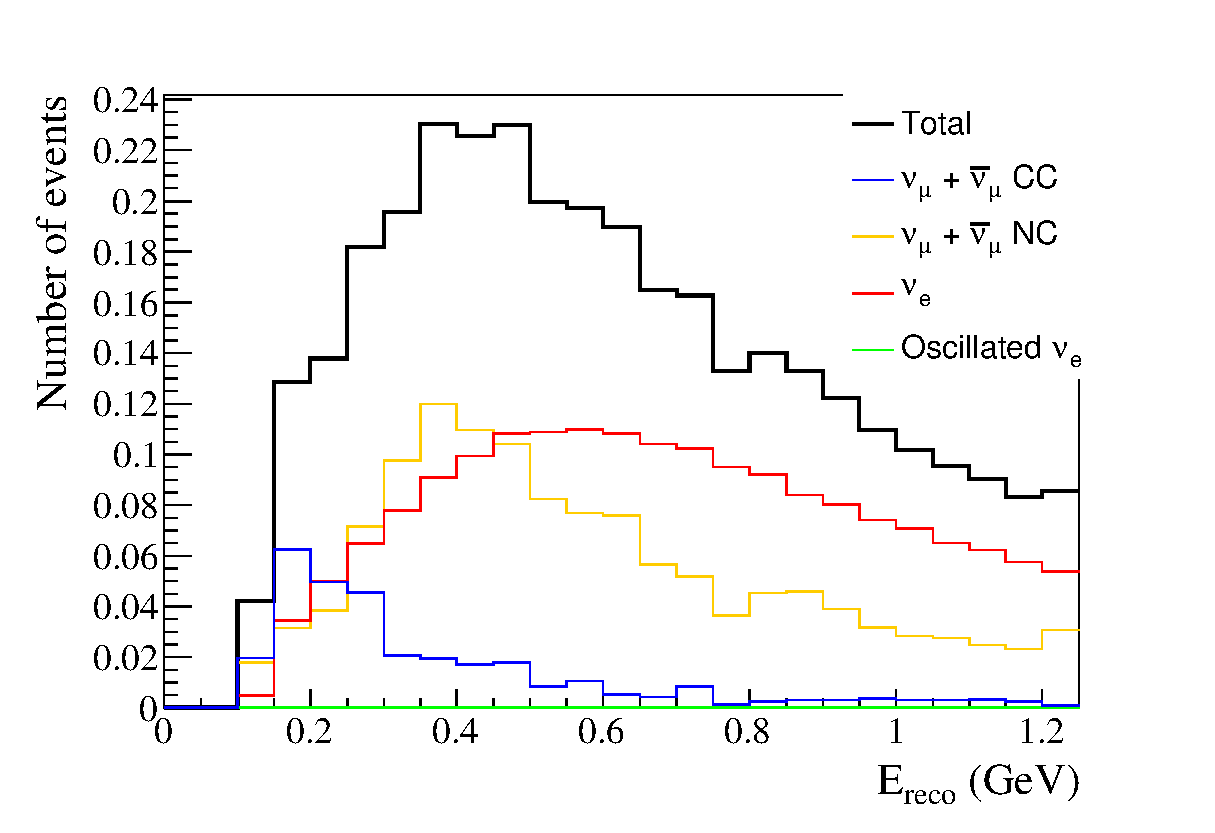
\includegraphics[width=20pc]{./images/prediction/1Re_spectrum_no_osc.eps}
\caption {
Predicted reconstructed-energy spectrum of single e-like ring events,
and contributions from various true neutrino reaction modes,
for no oscillations and
for an exposure of 3.010$\times$10$^{20}$ POT.
The 32 components of the spectrum are calculated separately in the actual analysis,
but, for this plot, are grouped into just four categories: 
$\nu_{\mu}$+$\bar{\nu}_{\mu}$ CC, $\nu_{\mu}$+$\bar{\nu}_{\mu}$ NC, $\nu_{e}$+$\bar{\nu}_{e}$ (intrinsic beam component)
and oscillated $\nu_{e}$.
The spectrum was generated using the BANFF-tuned MC templates.
}
\label{fig:1Re_spectrum_and_components_no_osc}
\end{minipage}
\end{figure*}

%...........
%
% 1Rmu, 1Re spectra - oscillations with typical parameters
%
\begin{figure*}[htb]
\begin{minipage}[t]{0.48\linewidth}
\center
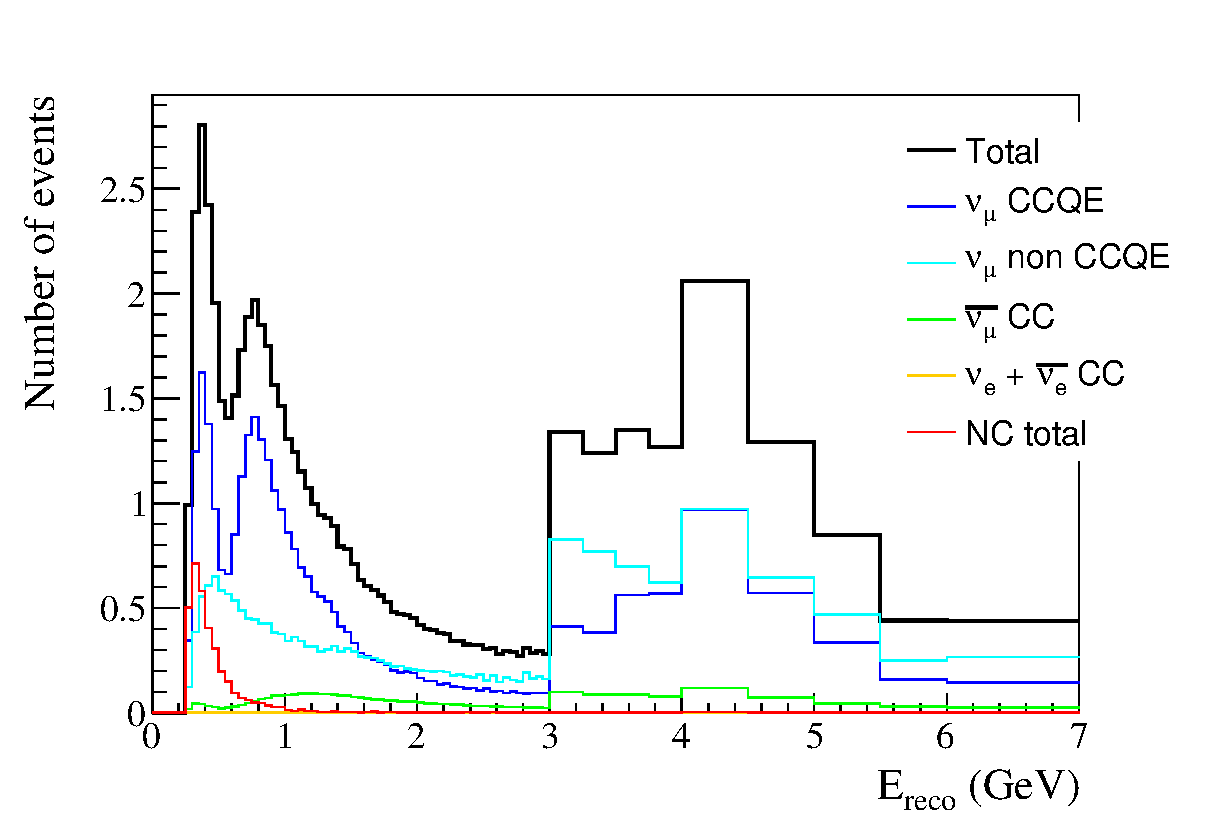
\includegraphics[width=20pc]{./images/prediction/1Rmu_spectrum_PDG.eps}
\caption {
Predicted reconstructed-energy spectrum of single $\mu$-like ring events,
and contributions from various true neutrino reaction modes,
for oscillations with $\sin^{2}\theta_{23}$=0.5 and $|\Delta m^{2}|$=2.4$\times$10$^{-3}$ eV$^{2}$/c$^{4}$
The spectrum was generated using the BANFF-tuned MC templates.
2012 PDG values are used for $\sin^{2}\theta_{13}$, $\sin^{2}\theta_{12}$ and $\delta m^{2}$,
while $\delta_{CP}$=0.
The spectrum shown was generated assuming the normal hierarchy.
Note that the vertical axis is zoomed in by a factor of 4 compared with Fig.\ \ref{fig:1Rmu_spectrum_and_components_no_osc}.
}
\label{fig:1Rmu_spectrum_and_components_default_osc}
\end{minipage}
\hspace{0.06\linewidth}
\begin{minipage}[t]{0.48\linewidth}
\center
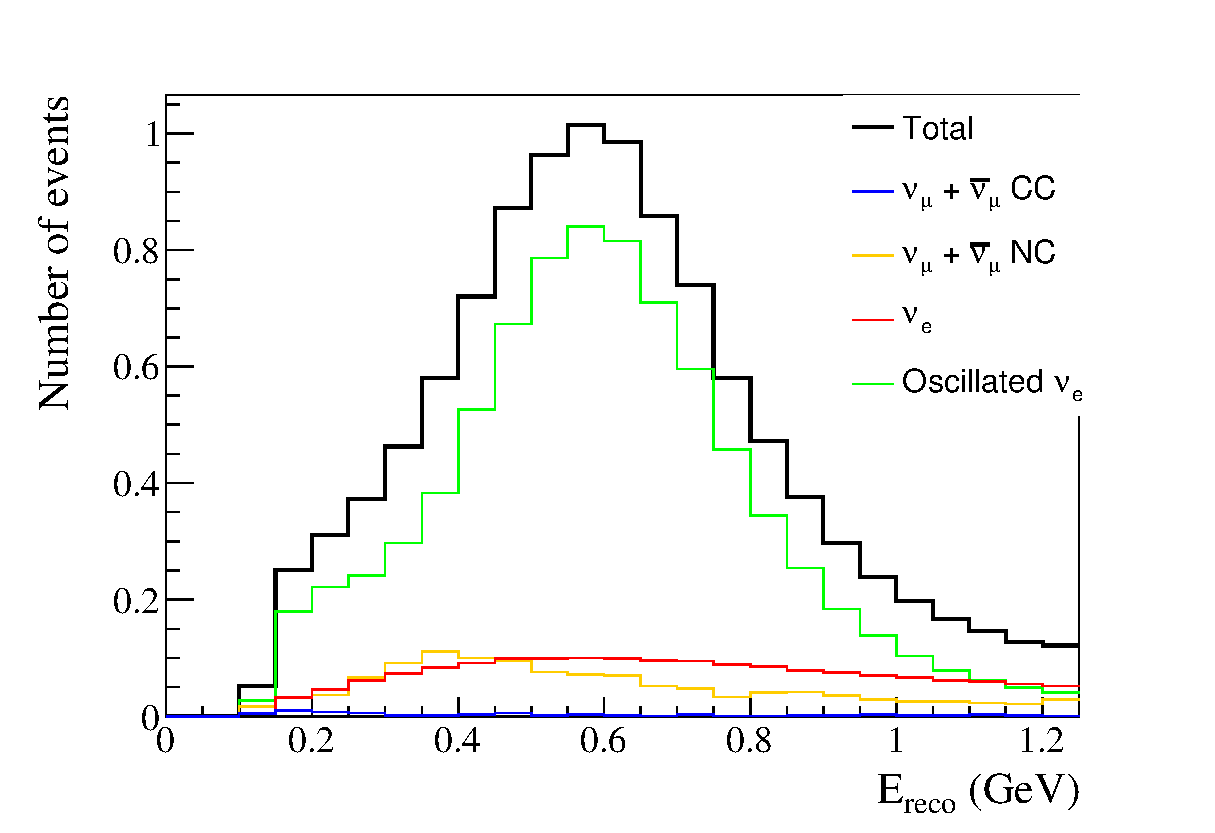
\includegraphics[width=20pc]{./images/prediction/1Re_spectrum_PDG.eps}
\caption {
Predicted reconstructed-energy spectrum of single e-like ring events,
and contributions from various true neutrino reaction modes,
for oscillations with $\sin^{2}\theta_{23}$=0.5, $|\Delta m^{2}|$=2.4$\times$10$^{-3}$ eV$^{2}$/c$^{4}$,
$\sin^{2}\theta_{13}$=0.098 and for an exposure of 3.010$\times$10$^{20}$ POT.
The spectrum was generated using the BANFF-tuned MC templates.
2012 PDG values are used for $\sin^{2}\theta_{12}$ and $\delta m^{2}$,
while $\delta_{CP}$=0.
The spectrum shown was generated assuming the normal hierarchy.
}
\label{fig:1Re_spectrum_and_components_default_osc}
\end{minipage}
\end{figure*}

%...........
%
% tables showing the effect of tunes on nsk and nsk components - no oscillations
%
\begin{table}
\centering
\begin{tabular}{| c || c | c | c || c | c | c | }
\hline  
                                                      & \multicolumn{6}{c|}{$N_{SK}$} \\
\hline  
                                                      & \multicolumn{3}{c||}{ single $\mu$-like ring} & \multicolumn{3}{c|}{ single e-like ring } \\
\hline  
                                                                               & Nominal  & NA61-tuned   & BANFF-tuned  & Nominal    & NA61-tuned   & BANFF-tuned    \\
\hline
Total &                                                                    190.986               &         210.465     &       204.624                 &     2.971      &      3.239        &       3.380           \\
\hline  
$\nu_\mu$ CCQE &                                                      151.820                    &     166.354         &      154.915         &     0.217      &        0.237      &       0.223           \\
$\nu_\mu$ CC 1$\pi$ &                                                             25.718        &       28.880       &         34.955      &   0.060        &    0.066          &        0.083          \\
$\nu_\mu$ CC coherent &                                                         0.898          &      1.005        &       0.950        &      0.0     &       0.0       &         0.0         \\
$\nu_\mu$ CC other &                                                              3.585        &     4.315         &          4.199     &        0.006   &     0.007         &      0.006            \\
$\nu_\mu$/$\nu_\tau$ NC 1$\pi^{+/-}$ ( 1R$\mu$ only)&             1.493               &    1.697          &      1.626         &    -      &      -       &       -          \\
$\nu_\mu$/$\nu_\tau$ NC 1$\pi^{0}$ (1R$_{e}$ only)&                            -     &      -       &      -        &    0.574       &     0.649         &       0.715           \\
$\nu_\mu$/$\nu_\tau$ NC coherent (1R$_{e}$ only)&                              -     &      -       &      -        &      0.193     &          0.218    &        0.208          \\
$\nu_\mu$/$\nu_\tau$ NC other &                                                  1.295         &      1.522        &       1.467        &      0.245     &        0.286      &       0.275           \\
$\bar{\nu}_{\mu}$ CCQE &                                                       4.119           &        4.460      &        3.978       &     0.002      &     0.002         &           0.002       \\
$\bar{\nu}_{\mu}$ CC 1$\pi$ &                                                   1.337          &       1.445       &      1.763         &    0.0004       &       0.0004       &     0.0005             \\
$\bar{\nu}_{\mu}$ CC coherent &                                          0.195                 &        0.211      &      0.203         &     0.0001      &      0.0001        &      0.0001            \\
$\bar{\nu}_{\mu}$ CC other &                                                     0.237         &         0.254     &        0.248       &      0.0     &     0.0         &        0.0          \\
$\bar{\nu}_{\mu}$/$\bar{\nu}_{\tau}$ NC 1$\pi^{+/-}$ (1R$\mu$ only) &    0.080       &    0.092          &      0.090         &    -      &      -       &       -          \\
$\nu_\mu$/$\nu_\tau$ NC 1$\pi^{0}$ (1R$_{e}$ only)&                           -      &      -       &      -        &     0.028      &       0.031       &      0.035            \\
$\nu_\mu$/$\nu_\tau$ NC coherent (1R$_{e}$ only)&                             -      &      -       &      -        &    0.018       &       0.020       &          0.019        \\
$\bar{\nu}_{\mu}$/$\bar{\nu}_{\tau}$ NC other &                                0.073           &       0.079       &        0.078       &   0.014        &     0.015         &        0.015          \\
$\nu_e$ CCQE &                                                            0.016                &       0.017       &        0.016       &     1.114      &        1.180      &           1.134       \\
$\nu_e$ CC 1$\pi$ &                                                       0.009                &        0.010      &        0.013       &      0.352     &       0.377       &         0.505         \\
$\nu_e$ CC coherent &                                                0.0004                     &     0.0004         &      0.0004         &      0.005     &      0.005        &          0.005        \\
$\nu_e$ CC other &                                                               0.003         &      0.003        &         0.003      &     0.028      &      0.030        &          0.029        \\
$\nu_e$ NC 1$\pi^{+/-}$ (1R$\mu$ only) &                            0.042            &      0.050        &      0.049         &    -      &      -       &      -           \\
$\nu_\mu$/$\nu_\tau$ NC 1$\pi^{0}$ (1R$_{e}$ only)&                           -      &      -       &      -        &      0.015     &    0.018          &        0.020          \\
$\nu_\mu$/$\nu_\tau$ NC coherent (1R$_{e}$ only)&                             -      &      -       &      -        &     0.004      &         0.005     &        0.005          \\
$\nu_e$ NC other &                                                                 0.005       &      0.057        &       0.057        &     0.009      &      0.010        &           0.010       \\
$\bar{\nu}_{e}$ CCQE &                                                        0.0008            &     0.0008         &       0.0008        &     0.052      &     0.052         &          0.051        \\
$\bar{\nu}_{e}$ CC 1$\pi$ &                                                            0.0006   &       0.0006       &      0.0007         &      0.021     &      0.021        &           0.029       \\
$\bar{\nu}_{e}$ CC coherent &                                                0.00007             &      0.00007        &        0.00007       &    0.004       &      0.004        &      0.004            \\
$\bar{\nu}_{e}$ CC other &                                                             0.0002   &        0.0002      &       0.0002        &    0.002       &    0.002          &          0.002        \\
$\bar{\nu}_{e}$ NC 1$\pi^{+/-}$ (1R$\mu$ only) &                0.006                &  0.006            &        0.006       &    -      &      -       &      -           \\
$\nu_\mu$/$\nu_\tau$ NC 1$\pi^{0}$ (1R$_{e}$ only)&                           -      &      -       &      -        &   0.002        &      0.002        &        0.002          \\
$\nu_\mu$/$\nu_\tau$ NC coherent (1R$_{e}$ only)&                             -      &      -       &      -        &      0.0009     &           0.0009   &         0.0009         \\
$\bar{\nu}_{e}$ NC other &                                                                &    0.006          &    0.006           &     0.001      &    0.001          &       0.001           \\
Oscillated $\nu_e$ CCQE &                                                             0          &          0    &        0       &       0    &          0    &         0         \\
Oscillated $\nu_e$ CC 1$\pi$ &                                                         0         &           0   &         0      &        0   &          0    &          0        \\
Oscillated $\nu_e$ CC coherent &                                                       0         &           0   &         0      &        0   &         0     &          0        \\
Oscillated $\nu_e$ CC other &                                                                0   &             0 &              0 &           0&            0  &              0    \\
\hline
\end{tabular}
\caption{
  Calculated numbers of single $\mu$-like ring and single e-like ring events without oscillations using the nominal MC templates, 
  the NA61-tuned MC templates and the BANFF-tuned MC templates.
  The total numbers of events and the numbers of events from each mode considered in this analysis are shown.
  These numbers were calculated for an exposure of 3.010$\times$10$^{20}$ POT.
  Note that different NC MC templates are used for predicting the number of single $\mu$-like ring and single e-like ring events.
}
\label{tab:nsk_nominal_x3_no_osc}
\end{table}


%...........
%
% tables showing the effect of tunes on nsk and nsk components - default oscillations
%
\begin{table}
\centering
\begin{tabular}{| c || c | c | c || c | c | c | }
\hline  
                                                      & \multicolumn{6}{c|}{$N_{SK}$} \\
\hline  
                                                      & \multicolumn{3}{c||}{ single $\mu$-like ring} & \multicolumn{3}{c|}{ single e-like ring } \\
\hline  
                                                                               & Nominal  & NA61-tuned   & BANFF-tuned  & Nominal    & NA61-tuned   & BANFF-tuned    \\
\hline
Total &                      54.264                                                             &  60.939            &  59.799             &  10.036         &  10.961            &  11.012                \\
\hline
$\nu_\mu$ CCQE &                                                                  30.926	&	34.183       &  30.962  	   &	0.028	    &	0.031		&	0.028		\\
$\nu_\mu$ CC 1$\pi$ &                                                             13.198	&	15.137       &  17.572  	   &	0.021	    &	0.023		&	0.029		\\
$\nu_\mu$ CC coherent &                                                            0.377	&	 0.434       &   0.412  	   &	0.000	    &	0.000		&	0.000		\\
$\nu_\mu$ CC other &                                                               3.210	&	 3.888       &   3.796  	   &	0.003	    &	0.003		&	0.003		\\
$\nu_\mu$/$\nu_\tau$ NC 1$\pi^{+/-}$ (1R$\mu$-like only)&                     1.492	&	 1.697       &   1.626  	   &	-      &      -       &       - 	 \\
$\nu_\mu$/$\nu_\tau$ NC 1$\pi^{0}$ (1R$_{e}$ only)&                            -     &      -       &      -        &   0.574	  &	0.649	      & 0.715		      \\
$\nu_\mu$/$\nu_\tau$ NC coherent (1R$_{e}$ only)&                              -     &      -       &      -        &   0.193	  &	0.218	      & 0.208		      \\
$\nu_\mu$/$\nu_\tau$ NC other &                                                    1.294       &	1.522	   &	1.466		&	0.248      &	0.286   	 &	0.274   	   \\
$\bar{\nu}_{\mu}$ CCQE &                                                           2.071       &	2.244	   &	1.936		&	0.0006      &	 0.0007 	  &	 0.0006 	    \\
$\bar{\nu}_{\mu}$ CC 1$\pi$ &                                                      0.976       &	1.053	   &	1.254		&	0.0002     &	0.0002  	 &	0.0002  	   \\
$\bar{\nu}_{\mu}$ CC coherent &                                                    0.107       &	0.116	   &	0.111		&	0.00007    &	0.00007 	 &	0.00007 	   \\
$\bar{\nu}_{\mu}$ CC other &                                                       0.211       &	0.226	   &	0.221		&	0.000      &	0.000   	 &	0.000   	   \\
$\bar{\nu}_{\mu}$/$\bar{\nu}_{\tau}$ NC 1$\pi^{+/-}$ (1R$\mu$ only) &    0.084       &	0.092	   &	0.090		&    -      &	   -	   &	   -	      \\
$\nu_\mu$/$\nu_\tau$ NC 1$\pi^{0}$ (1R$_{e}$ only)&                           -      &      -       &      -        &   0.028	  &	0.030	      & 0.034		      \\
$\nu_\mu$/$\nu_\tau$ NC coherent (1R$_{e}$ only)&                             -      &      -       &      -        &   0.018	  &	0.019	      & 0.018		      \\
$\bar{\nu}_{\mu}$/$\bar{\nu}_{\tau}$ NC other &                                    0.073 	&	0.079        &  0.077   	   &	0.013	    &	0.015		&	0.014		\\
$\nu_e$ CCQE &                                                                     0.014 	&	0.015        &  0.014   	   &	1.025	    &	1.085		&	1.042		\\
$\nu_e$ CC 1$\pi$ &                                                                0.008 	&	0.009        &  0.012   	   &	0.331	    &	0.355		&	0.476		\\
$\nu_e$ CC coherent &                                                              0.0004	&	0.0004       &  0.0003  	   &	0.004	    &	0.004		&	0.004		\\
$\nu_e$ CC other &                                                                 0.002 	&	0.003        &  0.002   	   &	0.026	    &	0.029		&	0.028		\\
$\nu_e$ NC 1$\pi^{+/-}$ (1R$\mu$ only) &                                 0.042 	&	0.048        &  0.048   	   &	 -     &      -       &       - 	 \\
$\nu_\mu$/$\nu_\tau$ NC 1$\pi^{0}$ (1R$_{e}$ only)&                           -      &      -       &      -        &   0.015	  &	0.017	      & 0.020		      \\
$\nu_\mu$/$\nu_\tau$ NC coherent (1R$_{e}$ only)&                             -      &      -       &      -        &   0.004	  &	0.005	      & 0.004		      \\
$\nu_e$ NC other &                                                                0.049  	 &	0.057          & 0.057   	      & 0.009	       &	0.010	   &	0.010		   \\
$\bar{\nu}_{e}$ CCQE &                                                            0.0008 	 &	0.0007         &0.0007  	      & 0.048	       &	0.048	   &	0.047		   \\
$\bar{\nu}_{e}$ CC 1$\pi$ &                                                       0.0006 	 &	0.0005         &0.0007  	      & 0.020	       &	0.020	   &	0.027		   \\
$\bar{\nu}_{e}$ CC coherent &                                                     0.00007	 &	0.00007        &0.00007 	      & 0.003	       &	0.003	   &	0.003		   \\
$\bar{\nu}_{e}$ CC other &                                                        0.0002 	 &	0.0002         &0.0002  	      & 0.002	       &	0.001	   &	0.001		   \\
$\bar{\nu}_{e}$ NC 1$\pi^{+/-}$ (1R$\mu$ only) &                        0.006  	 &	0.005          &0.005   	      &    -	  &	 -	 &	 -	    \\
$\nu_\mu$/$\nu_\tau$ NC 1$\pi^{0}$ (1R$_{e}$ only)&                           -      &      -       &      -        &  0.001 	   &	0.001   	&	0.002   	 \\
$\nu_\mu$/$\nu_\tau$ NC coherent (1R$_{e}$ only)&                             -      &      -       &      -        &  0.0009	   &	0.0009  	&	0.0009  	 \\
$\bar{\nu}_{e}$ NC other &                                                        0.006  	 &	0.005        & 	0.006       &	0.001	     &  0.001		 &	0.001		 \\
Oscillated $\nu_e$ CCQE &                                                         0.080  	       &0.088   	    &	0.083   	  &	6.378	   &	6.965	       &	6.567	       \\
Oscillated $\nu_e$ CC 1$\pi$ &                                                    0.025  	       &0.026   	    &	0.034   	  &	0.996	   &	1.090	       &	1.406	       \\
Oscillated $\nu_e$ CC coherent &                                                  0.002  	       &0.002   	    &	0.001   	  &	0.020	   &	0.022	       &	0.021	       \\
Oscillated $\nu_e$ CC other &                                                     0.0006 	       &0.0006  	    &	0.0006  	  &	0.014	   &	0.015	       &	0.014	       \\
\hline
\end{tabular}
\caption{
  Calculated numbers of single $\mu$-like ring and single e-like ring events with oscillations
  using the nominal MC templates, the NA61-tuned MC templates and the BANFF-tuned MC templates.
  The total numbers of events and the numbers of events from each mode considered in this analysis are shown.
  These numbers were calculated for an exposure of 3.010$\times$10$^{20}$ POT 
  and oscillations with $\delta_{CP}$=0, $\sin^{2}\theta_{13}$=0.025, $\sin^{2}\theta_{23}$=0.5 and $|\Delta m^{2}|$=2.4$\times$10$^{-3}$ eV$^{2}$/c$^{4}$.
  The 2012 PDG parameters are used for $\sin^{2}\theta_{12}$ and $\delta m^{2}$.
  The normal hierarchy is assumed.
  Note that different NC MC templates are used for predicting the number of single $\mu$-like ring and single e-like ring events.
}
\label{tab:nsk_nominal_x3_default_osc}
\end{table}










\clearpage

\section{Systematic effects in the prediction of the single $\mu$-like ring and single e-like ring event reconstructed energy spectra in SuperK}
%\section{Updated systematic effects in the prediction of the single $\mu$-like ring and single e-like ring event reconstructed energy spectrum}
\label{sec:systematics}

There are 64 systematic parameters considered in this analysis. 
They will be described now, grouped into 4 categories:

\begin{enumerate}

%%%% ENERGY SCALE 

\item 
{\bf SuperK energy scale} (1 parameter).\\
The systematic parameter $f_{E; r}^{SK}$ is included to account for the energy scale uncertainty, 
which is estimated to be 2.4\% \cite{SuperkEScale2013}.
This systematic parameter is applied differently to the other systematics, since it is not applied as a weight in the number of events in each bin. 
The effect of the uncertainty in the reconstructed energy scale is computed by scaling the bin edges of
the MC templates and, assuming uniform distribution of events within the bins, calculating the number
of events gained from / lost to neighbouring bins. 
The effect of the energy scale uncertainty is propagated to all MC templates as shown in Tab.\ \ref{tab:apply_syst_to_1Rmu_templates} and \ref{tab:apply_syst_to_1Re_templates}.\\


%%%% SK + FSI + SI 

\item 
{\bf SuperK efficiencies \& effects of intranuclear and secondary re-interactions \& Photo nuclear effects } (6+12 parameters).\\

There are uncertainties in the efficiencies of the cuts used to select single ring events at SuperK: the fiducial volume and reduction chain, and the OD, ring-counting, PID, momentum and decay-electron cuts.
These uncertainties are evaluated comparing SK-IV atmospheric data with atmospheric neutrino Monte Carlo.
For the 2013 joint oscillation analysis, these uncertainties were evaluated taking into account correlations between
the two single $\mu$-like ring and single e-like ring event samples \cite{SKcorrelations}.
Very pure samples of atmospheric neutrinos with either single $\mu$-like ring or single e-like ring events at the final state were selected. Those samples are fitted to the data including constraints from control samples (stopping cosmic muons and hybrid $\pi^0$ samples), using a Markov-Chain Monte Carlo method with the efficiencies as fit parameters (see details in \cite{PatrickPlenary}).
Finally, the covariance matrix is calculated using toy MC experiments as explained in \cite{ImberTalk}. 

Intranuclear final-state interactions (FSI) have significant effects in the T2K energy range and
result in event topologies, for scattering from nuclear targets, which are drastically different from 
those created in neutrino scattering from free nucleons.
Uncertainties due to FSI were estimated by simultaneously varying the NEUT parameters that scale the interaction probabilities for quasi-elastic 
scattering, absorption, charge exchange and pion production using the method described in Sec.\ 2 in \cite{NIWGErr}. 
Uncertainties due to secondary pion interactions (SI) were also evaluated. Since the same model is used for FSI and SI, it is possible to evaluate the uncertainties in both FSI and SI simultaneously. 
For each stand-alone analysis, $\nu_{\mu}$ disappearance or $\nu_{e}$ appearance analysis, the same set of 8 FS+SI  parameters is used. 
The effect of FSI+SI uncertainties is estimated by reweighting at the same time single $\mu$-like ring and single e-like selected SK MC events 
with the same 8 parameters set for both samples using T2KReweight, and finding the number of events in each one of the 18 event categories 
(6 categories in $\nu_{\mu}$ disappearance and 12 categories $\nu_{e}$ appearance, the same as the final parametrization of SK+FSI+SI parameters).
The reweighting method for FSI is described in Sec. 8 in \cite{NEUTnuclear}. Variations in the SI interaction probabilities were included for each FSI parameter set. 
Subsequently a covariance matrix was calculated using equation 1 in \cite{NIWGErr}; the quantity p in that equation is the average event weight for a FSI parameter set, and 
the sum is over the parameter sets. This covariance matrix contains correlations between the two single $\mu$-like ring and single e-like ring events samples \cite{ikeda}.

For this analysis, systematic errors related to Photo Nuclear effects (interactions between photons and nuclei) were taken into account following the work done for the stand-alone appearance analyses. The identification of a $\pi^0$ relies on the detection of the two photons produced by this particle, but a photon can be absorbed before emitting Cerenkov light, being therefore undetected, and this would create an additional uncertainty for the interaction modes where a $\pi^0$ is produced. 
A covariance matrix has been calculated for the PN uncertainty using the fiTQun $\pi^0$ cut, in the same binning used for the stand-alone appearance analysis SK and FSI systematic errors \cite{2013nueptheta}, \cite{2013nuenergy}.

In this analysis,the SuperK detector efficiency and FSI+SI systematics are considered together, adding their covariance matrices linearly, what it is possible since the same binning is used for both covariance matrices. Then, the PN covariance matrix is added linearly to the SK+FSI submatrix (12 x 12) related to the single e-like ring sample. Details of these uncertainties are given in 
Tab.\ \ref{tab:input_uncertainties}, and the final SK+FSI+SI+PN covariance matrix and fractional errors are presented in \ref{eq:Cskfsi} and \ref{fig:skfsi_frac} respectively. These efficiency/FSI/SI systematics are applied to the MC templates as shown in Tab.\ \ref{tab:apply_syst_to_1Rmu_templates} and \ref{tab:apply_syst_to_1Re_templates}.\\

%%%%% BANFF

\item 
{\bf Correlated flux and cross-section (BANFF) parameters} (33 parameters).\\

The postfit uncertainties of all BANFF flux and cross-section parameters and their correlations are taken into account.
The version of the BANFF fit is slightly different for the stand-alone disappearance, stand-alone appearance and joint oscillation analyses. 
Concerning the flux parameters, for the stand-alone disappearance analysis the version of the BANFF fit considers only the $\nu_\mu$ and $\bar{\nu}_{\mu}$ flux parameters, whereas for the stand-alone appearance flux parameters are considered for $\nu_\mu$, $\bar{\nu}_{\mu}$, $\nu_e$ and $\bar{\nu}_{e}$, with a smaller number of $\bar{\nu}_{\mu}$ flux bins than the stand-alone disappearance analysis. The BANFF version for the joint analysis includes flux bins for $\nu_\mu$, $\bar{\nu}_{\mu}$, $\nu_e$ and $\bar{\nu}_{e}$, with the number of flux bins for $\bar{\nu}_{\mu}$ from the stand-alone disappearance analysis. 
There are also differences in the number of correlated cross-section parameters included in the different BANFF versions for the stand-alone analyses and the joint analysis. For the stand-alone disappearance analysis, there are three CCQE normalization parameters (0-1.5 GeV, 1.5-3.5 GeV and 3.5-30 GeV) and two for the CC1$\pi$ normalization (1.5-3.5 GeV and 3.5-30 GeV), whereas for the stand-alone appearance analysis only one parameter is consider for each normalization, the one in the lower energy range. There is also one extra parameter in the stand-alone appearance analysis with respect to the stand-alone disappearance analysis: this is the NC1$\pi^{0}$ normalization parameter. The BANFF version produced for the joint analysis considers all the cross-section parameters included in the stand-alone disappearance and stand-alone appearance versions (8 in total), however, the NC1$\pi^{0}$ normalization parameter is only applied to the single e-like ring sample templates, because there are no single $\mu$-like ring NC1$\pi^{0}$ templates.

A summary of the list of parameters included in the BANFF postfit files for each oscillation analysis is given in Tab. \ref{tab:banff}

\begin{table}[h]
\centering
\begin{tabular}{|c||c|c|c|}
\hline
Parameter & $\nu_{\mu}$-disappearance analysis & $\nu_{e}$-appearance analysis  & joint analysis\\
\hline \hline
\multirow{4}{*}{$\nu_{\mu}$ flux} & 0-0.4, 0.4-0.5, 0.5-0.6, &  0-0.4, 0.4-0.5, 0.5-0.6, &   0-0.4, 0.4-0.5, 0.5-0.6,\\
 & 0.6-0.7, 0.7-1.0, 1.0-1.5, & 0.6-0.7, 0.7-1.0, 1.0-1.5, & 0.6-0.7, 0.7-1.0, 1.0-1.5, \\
 & 1.5-2.5, 2.5-3.5, 3.5-5.0,  & 1.5-2.5, 2.5-3.5, 3.5-5.0,  & 1.5-2.5, 2.5-3.5, 3.5-5.0, \\
&  5.0-7.0, 7.0-30.0 \bf{(11 bins)}  &  5.0-7.0, 7.0-30.0 \bf{(11 bins)}  &  5.0-7.0, 7.0-30.0 \bf{(11 bins)} \\
\hline
\multirow{2}{*}{$\bar{\nu_{\mu}}$ flux }& 0-0.7, 0.7-1.0, 1.0-1.5, &  0-1.5, 1.5-30.0 \bf{(2 bins)}  & 0-0.7, 0.7-1.0, 1.0-1.5,\\
& 1.5-2.5, 2.5-30.0 \bf{(5 bins)} & & 1.5-2.5, 2.5-30.0 \bf{(5 bins)}\\
\hline
\multirow{3}{*}{$\nu_{e}$ flux} & -- &  0-0.5, 0.5-0.7, 0.7-0.8, & 0-0.5, 0.5-0.7, 0.7-0.8, \\
& & 0.8-1.5, 1.5-2.5, 2.5-4.0, & 0.8-1.5, 1.5-2.5, 2.5-4.0, \\
& &  4.0-30.0 \bf{(7 bins)} &  4.0-30.0 \bf{(7 bins)} \\
\hline
$\bar{\nu_{e}}$ flux & -- & 0-2.5, 2.5-30.0 \bf{(2 bins)} & 0-2.5, 2.5-30.0 \bf{(2 bins}) \\
\hline \hline
$M_{A}^{QE}$ & \ck & \ck & \ck \\
\hline
$M_{A}^{RES}$ & \ck & \ck & \ck\\
\hline
CCQE normalization (0-1.5 GeV) & \ck & \ck & \ck\\
\hline
CCQE normalization (1.5-3.5 GeV) & \ck & -- & \ck\\
\hline
CCQE normalization (3.5-30. GeV) & \ck & -- & \ck\\
\hline
CC1$\pi$ normalization (0-2.5 GeV) & \ck & \ck & \ck\\
\hline
CC1$\pi$ normalization (2.5-30 GeV) & \ck & -- & \ck\\
\hline
NC1$\pi^{0}$ normalization & -- & \ck & \ck\\
\hline
\end{tabular}
\caption{List of parameters included in the BANFF postfit files, varying depending on the different versions produced for each oscillation analysis.}
\label{tab:banff}
\end{table}

%{tab:apply_syst_to_samples}


A list of the BANFF parameters, their best-fit values and their prefit and postfit errors is given in Tab.\ \ref{tab:input_uncertainties} and Fig. \ref{fig:banff}.

The BANFF parameters are applied to the MC templates as specified in Tab.\ \ref{tab:apply_syst_to_1Rmu_templates} and \ref{tab:apply_syst_to_1Re_templates}.
Among the BANFF cross-section parameters, all but two are simple normalization factors. 
However, the parameters $f_{25; t, r}^{banff}$ and $f_{26; t, r}^{banff}$, the ones corresponding to the 
axial masses ( CC quasi-elastic, $M_{A}^{QE}$, and resonance-production, $M_{A}^{RES}$ respectively), have a more complicated, often non-linear, dependence on true and reconstructed neutrino energy.
For this reason, event reweighting methods were used to obtain the fractional changes of the number of events
in bins of true and reconstructed neutrino energy, for a range of values (-3.0$\sigma$, -2.5$\sigma$, -2.0$\sigma$, ..., +3.0$\sigma$) for the $f_{25; t, r}^{banff}$ and $f_{26; t, r}^{banff}$ parameters.
In our p.d.f. calculation, cubic splines

\footnote{
  In this analysis, as in the \textit{VALOR} stand-alone disappearance analysis \cite{OurRun1234DisappAnalysis3Flavour},
 the cubic splines are computed for each non-linear systematic and for each MC template,
  in bins of reconstructed and true energy. To produce these splines, the SK13a SuperK MC, the 11bv3.2 flux weights are used and the following oscillation parameters: $\sin^{2}(2\theta_{23})$ = 1.0, $\sin^{2}(2\theta_{13})$ = 0.098, $\sin^{2}(2\theta_{12})$ = 0.8495, $|\Delta m^{2}_{32}|$ = 2.44$\times$10$^{-3}$ eV$^{2}$/c$^{4}$, $\Delta m^{2}_{21}$ = 7.5$\times$10$^{-5}$ eV$^{2}$/c$^{4}$, $\delta_{CP}$ = 0 and the normal mass hierarchy. 
The splines for the single $\mu$-like ring sample were made using 41 bins in reconstructed energy:
  1 bin from 0-0.3 GeV, 14 50-MeV bins from 0.3-1.0 GeV, 20 100-MeV bins from 1.0-3.0 GeV, 2 500-MeV bins from 3.0-4.0 GeV, 1 bin from 4.0-5.0 GeV, 1 bin from 5.0-7.0 GeV, 1 bin from 7.0-10.0 GeV and 1 bin from 10.0-30.0 GeV.
  The $\nu_{\mu}$, $\bar{\nu}_{\mu}$ and oscillated $\nu_{e}$ selections for the single $\mu$-like ring sample have 11 bins in true energy:
  1 bin from 0-0.4 GeV, 3 100-MeV bins from 0.4-0.7 GeV, 1 bin from 0.7-1.0 GeV, 1 bin from 1.0-1.5 GeV, 2 1-GeV bins from 1.5-3.5 GeV,  1 bin from 3.5-5.0 GeV, 1 bin from 5.0-7.0 GeV and 1 bin from 7.0-30.0 GeV, 
and the $\nu_{e}$ and oscillated $\nu_\mu$ samples have 7 bins in true energy:
  1 bin from 0-0.05 GeV, 1 bin from 0.5-0.7 GeV, 1 bin from 0.7-0.8 GeV,
  1 bin from 0.8-1.5 GeV, 1 bin from 1.5-2.5 GeV, 1 bin from 2.5-4.0 GeV and 1 bin from 4.0-30.0 GeV,
  and finally, the $\bar{\nu}_{e}$ sample have 2 bins in true energy:
  1 bin from 0-2.5 GeV and 1 bin from 2.5-30.0 GeV. The binning of the cubic splines for the single $\mu$-like ring events was studied, and the results were presented in Appendix I of \cite{OurRun123DisappAnalysis3Flavour}. \\
For the single e-like ring sample splines the reconstructed and true energy bins used were the same ones used for the
stand-alone appearance analyses. Therefore, reconstructed energy bins of 50 MeV were used from 0-1.25 GeV for $\nu_{\mu}$, $\bar{\nu}_{\mu}$,$\nu_{e}$, $\bar{\nu}_{e}$ and oscillated $\nu_{e}$. The binning for true energy for the single e-like ring events coincide with the one used for the single $\mu$-like ring events, with the exception of the oscillated $\nu_{e}$ sample, which uses in the single e-like ring sample the following 7 bins in true energy:
  1 bin from 0-0.05 GeV, 1 bin from 0.5-0.7 GeV, 1 bin from 0.7-0.8 GeV,
  1 bin from 0.8-1.5 GeV, 1 bin from 1.5-2.5 GeV, 1 bin from 2.5-4.0 GeV and 1 bin from 4.0-30.0 GeV.
  The spline spectra produced using the cubic splines are very similar to those produced using the CPU-intensive event-by-event reweighting, especially for the dominant components of the spectra. 
} are used to interpolate between these event weights 
to obtain the fractional change for any value of these systematic parameters in the (-3.0$\sigma$, +3.0$\sigma$) range.
An example of one cubic spline is presented in Fig. \ref{fig:spline}.\\

%% SPLINE EXAMPLE PLOT
\begin{figure*}[htb]
\center
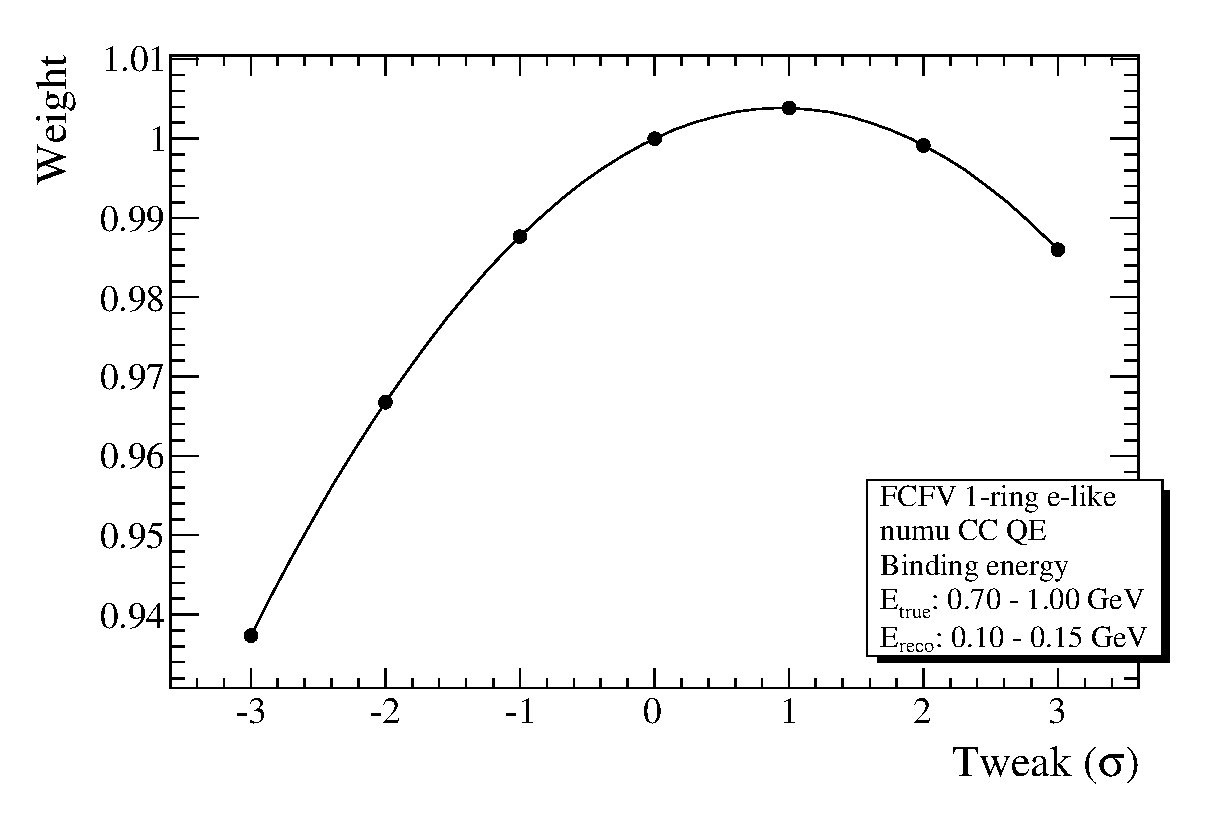
\includegraphics[width=30pc]{./images/systematics/spl_1Re_numuccqe_f_bindE_3_4.eps}
\caption {
  Example of response function (cubic spline) showing the weight vs the tweak for the Binding Energy systematic parameter
for the 1R$_e$ sample, $\nu_{\mu}$ CCQE interaction mode, $E_{true}$ between 0.7-1.0 GeV and $E_{reco}$ between 0.10-0.15 GeV.
}
\label{fig:spline}
\end{figure*}



%%% UNCORRELATED CROSS SECTIONS

\item 
{\bf Uncorrelated cross-section parameters}(12 parameters).\\

In addition to the BANFF cross-section systematics,
another 12 cross-section systematics are taken into account; these additional systematics are considered to be uncorrelated 
between themselves and to have no cancellation between the near and far detectors \cite{NIWGErr} \cite{MoreNIWGErr113} \cite{NIWGNuBarErr}.

There are some differences in the list of uncorrelated cross-section parameters between the different oscillation analyses. 
There is one systematic parameter which is only consider in the stand-alone appearance analysis, but not in the stand-alone disappearance analysis: this is the NC coherent cross-section parameter. On the other hand, there are three cross-section systematics that are used in the stand-alone disappearance analysis but not in the stand-alone appearance analysis: the systematic for the Binding Energy, the NC1$\pi^{\pm}$ cross-section and the $\sigma_{\bar{\nu}}/\sigma_{\nu}$ ratio. The joint oscillation analysis considers them all (12 parameters) although the NC coherent cross-section parameter is only applied to the single e-like ring NC coherent templates (there are no single $\mu$-like ring NC coherent templates) and the  NC1$\pi^{\pm}$ cross-section parameter is only applied to the single $\mu$-like ring NC1$\pi^{\pm}$ templates (there are no single e-like ring NC1$\pi^{\pm}$ templates).

Three of these additional systematics relate to the initial-state nuclear environment modeling for CCQE.
Neutrino Monte Carlo generators typically use Relativistic Fermi Gas (RFG) models,
with or without extensions to take nucleon-nucleon correlation into account, 
and with some, often simplistic, prescription for the treatment of off-shell kinematics.
The RFG model implementation depends on two parameters, the Fermi momentum level (225 MeV for $^{16}O$)
and the nucleon binding energy (27 MeV for $^{16}O$), which are extracted from quasi-elastic electron scattering data.
The systematic parameter $f_{pF; t, r}$ takes into account the effect of a 30 MeV 1$\sigma$ uncertainty in the Fermi momentum level
for $^{16}O$, while the parameter $f_{bindE; t, r}$ takes into account the effect of a 9 MeV 1$\sigma$ uncertainty in the nucleon 
binding energy for for $^{16}O$.
The implementation details of the nuclear model can have a significant effect and, therefore,
the effect of switching between two such models was also included as a systematic uncertainty.
This analysis considers the effect of switching between the RFG model and a better-motivated 
Spectral Function (SF) model. The latter does not assume a fixed binding energy and includes the 
correlations between nucleon momentum and binding energy. The systematic parameter $f_{SF; t, r}$ 
includes the effect of switching between the two models.
Thus, the systematic parameter $f_{SF; t, r}$  needs an special treatment. After discussions with 
the NIWG group, the latest recommendation is followed in this analysis (see below), and the effect
of the change in its treatment means a big difference as it is shown in Sec. \ref{app:standalone}.


Simple, energy-independent, generator-level uncertainties are considered for the CC coherent, NC, $\sigma_{\nu_{e}}/\sigma_{\nu_{\mu}}$ ratio and $\sigma_{\bar{\nu}}/\sigma_{\nu}$ ratio cross sections.
This analysis uses a 100\% uncertainty for the CC coherent cross-section, 
a 30\% uncertainty for both the NC1$\pi^\pm$, NC coherent and NC ``other''  cross section,
a 3\% uncertainty on the $\nu_e$ / $\nu_\mu$ CC cross-section ratio and 
a 20\% uncertainty on the $\bar{\nu}$ / $\nu$ CC cross-section ratio.

The effect of the variation of the above cross sections is included in the analysis
through the systematic parameters $f_{CCcoh; t}$, $f_{NC1\pi^\pm; t}$, $f_{NCcoh; t}$, $f_{NCoth; t}$,
$f_{CC\nu_e; t}$ and $f_{CC\bar{\nu}; t}$ respectively.

The treatment of $\Delta$ resonances in the nuclear environment has been controversial in the neutrino
Monte Carlo generator community. Certain models include a ~20\%-level of $\pi$-less $\Delta$ decays in order
to include the effect of $\Delta+N \rightarrow N+N$ scattering, in which the $\Delta$ interacts before it can decay. 
In contrast, other models include no $\pi$-less 
$\Delta$ decays on the basis that this would amount to double counting since, whatever the size of the effect, 
it is already included in hadron-nucleus scattering data to which the intranuclear cascade Monte Carlos are tuned.
This analysis uses NEUT, in which 20\% of $\Delta$s have a $\pi$-less decay by default, and takes the uncertainty in this 
branching fraction to be 100\%. 
The systematic parameter $f_{\pi-less\Delta; t, r}$ includes the effect of varying the fraction of $\pi$-less $\Delta$ 
decays to the corresponding MC templates.

The $f_{CCothShape;t,r}$ systematic parameterizes the uncertainty in CC multi-pion, CC deep inelastic scattering and CC $\eta$, K and photon production. 
From MINOS data, this is known to be $\approx$10\% at 4 GeV. Using this as a reference point, 
the uncertainty is estimated as 0.4/E$_{\nu}$, where E$_{\nu}$ is in GeV. It might appear that this error could diverge at 
low energy, but this does not happen since the threshold is $\approx$0.6 GeV and there are very 
few interactions below 1 GeV. 

The $f_{Wshape;t,r}$ parameter modifies the shape of the initial pion momentum distribution (before final-state interactions) 
by changing the distribution of the pion/nucleon invariant mass while keeping the total cross section constant. As the 
W shape parameter decreases, the pion momentum shifts to lower values, and this increases the probability of pion 
absorption in a final-state interaction. If such an absorption occurs, the event is migrated from CC1$\pi$ (its 
true initial state) and appears to be CCQE.

The effect of the $f_{CCcoh; t}$, $f_{NC1\pi^\pm; t}$, $f_{NCcoh; t}$, $f_{NCoth; t}$, $f_{CC\nu_e; t}$ and $f_{CC\bar{\nu}; t}$ 
systematic parameters is a simple normalisation change for the corresponding MC templates and thus easily implemented.
Systematic parameters $f_{pF; t, r}$, $f_{SF; t, r}$, $f_{bindE; t, r}$, $f_{\pi-less\Delta; t, r}$, $f_{CCothShape; t, r}$ 
and $f_{Wshape; t, r}$  have a complicated, often non-linear, dependence on true and reconstructed energy.
These are treated in a similar way to the BANFF parameters $f_{25; t, r}^{banff}$ and $f_{26; t, r}^{banff}$.
Event reweighting methods were used to obtain the fractional changes of the number of events, 
in bins of true and reconstructed neutrino energy, for a range of values (-3.0$\sigma$, -2.5$\sigma$, -2.0$\sigma$, ..., +3.0$\sigma$) of the systematic parameters. 
Again cross-section splines with polynomials of order 3 were used to interpolate between these event 
weights to obtain the fractional change for any value of these systematic parameters in the (-3.0$\sigma$, +3.0$\sigma$) range.

Some of these systematics are special cases:
{
\begin{itemize}
\item 
  $f_{SF; t, r}$ is discrete; it can be either spectral function off (RFG) or spectral function on (SF). 
  Splines are generated with SF off as nominal (0), and SF on as +1$\sigma$.
  This parameter is restricted to the range between 0 and +1$\sigma$, and linear interpolation is made between the weights 
  for nominal and +1$\sigma$.
\item 
  For $f_{Wshape; t, r}$ only $\pm$1$\sigma$ errors are evaluated using event reweighting. 
  Weights for positive tweaks are interpolated or extrapolated from the nominal and +1$\sigma$ weights, and weights for negative tweaks are interpolated or extrapolated from the nominal and -1$\sigma$ weights.
\item 
  For $f_{\pi-less\Delta; t, r}$ only $\pm$1.0 sigma errors are evaluated using event reweighting.
  Weights for positive tweaks are interpolated or extrapolated from the nominal and +1$\sigma$ weights, and weights for tweaks between nominal and -1$\sigma$ are interpolated from the nominal and -1$\sigma$ weights. Weights for tweaks more negative than -1$\sigma$ are taken to be the same as the -1$\sigma$ weight; this is done since 20\% of $\Delta$s have a $\pi$-less decay by default in NEUT, and the error is 20\%. For this reason, it is unphysical to tweak $f_{\pi-less\Delta; t, r}$ to be more negative than -1$\sigma$. 
\end{itemize}
}

The 12 uncorrelated cross-section systematics considered in this analysis are summarised in Tab.\ \ref{tab:input_uncertainties}.
These cross-section systematics are applied to the MC templates as shown in Tab.\ \ref{tab:apply_syst_to_1Rmu_templates} and \ref{tab:apply_syst_to_1Re_templates}.\\

\end{enumerate}

Table \ref{tab:apply_syst_to_samples} presents a summary of which systematic parameter is applied to each sample (single $\mu$-like ring or single e-like ring) for the stand-alone and the joint analyses. 





% ................................................................................................................

%
% Table summarizing systematics
%
\clearpage
{
\small
\renewcommand{\arraystretch}{2.0} % enlarge line spacing
\begin{longtable}{p{1.65cm}l}
%
% SuperK & FSI+SI
%
\hline
\multicolumn {2}{l} { {\bf SuperK energy scale systematics (1)} } \\
\hline
  \parbox{0.15\textwidth}
  {
    $f_{E; r}^{SK}$ 
  }
& 
  \parbox{0.81\textwidth}
  {
    \vspace{0.2cm}
    Reconstructed energy scale systematic.
    The uncertainty is estimated to be 2.4\% \cite{SuperkEScale2013}.
    \vspace{0.2cm}
  }
\\
\hline
\multicolumn {2}{l} { {\bf SuperK detector efficiency \& intranuclear and
    secondary interaction and phononuclear systematics (18)} } \\
\hline
  \parbox{0.15\textwidth}
  {
     $f_{i; r}^{SK+FSI}$
  }
&
  \parbox{0.81\textwidth}
  {
    \vspace{0.2cm}
    SuperK detector efficiency (ring counting, fiducial volume, reduction chain, OD cut, PID cut, momentum cut and 
    decay electron cut efficiency uncertainties), 
    FSI (final state interaction / intranuclear hadron transport) and
    SI (secondary interaction / detector hadron transport) 
    and PN (photo nuclear/ interactions between photons and nuclei) systematic parameters.
    Eighteen correlated parameters are included (i=0,...,17) corresponding to different modes and reconstructed energy bins.\\
    $$     
        {
         \renewcommand{\arraystretch}{1.0} % enlarge line spacing
         \begin{array}{c|c|c}
            \text{Parameter} & \text{Description} & 1\sigma \text{ fractional error} \\
            0 & \text{1R$_{\mu}$, \ \ } \nu_\mu \text{ \& } \bar{\nu}_{\mu} \text{ CCQE, } E_{reco} < \text{ 0.4 GeV}                              & 0.0199   \\
            1 &  \text{1R$_{\mu}$,\ \ } \nu_\mu \text{ \& } \bar{\nu}_{\mu} \text{ CCQE, } \text{0.4 GeV} \leq E_{reco} \leq \text{ 1.1 GeV}       & 0.0193   \\
            2 &  \text{1R$_{\mu}$,\ \ } \nu_\mu \text{ \& } \bar{\nu}_{\mu} \text{ CCQE, } E_{reco} > \text{ 1.1 GeV}                              & 0.0199   \\
            3 &  \text{1R$_{\mu}$,\ \ } \nu_\mu \text{ \& } \bar{\nu}_{\mu} \text{ CCnonQE}                                                        & 0.0933  \\
            4 &  \text{1R$_{\mu}$,\ \ }  \nu_e \text{ \& } \bar{\nu}_{e} \text{ CC}                                                                 & 1.005   \\
            5 & \text{1R$_{\mu}$,\ \ } \text{All NC}                                                                                              & 0.599   \\
	    6 &  \text{1R$_{e}$,\ \ } osc. \nu_e \text{ CC} E_{reco} < \text{ 0.35 GeV}                      &  0.110 \\
            7 &  \text{1R$_{e}$,\ \ }  osc. \nu_e \text{ CC}     \text{0.35 GeV} \leq E_{reco} \leq \text{ 0.8 GeV}                 &  0.0309 \\	
            8 &  \text{1R$_{e}$,\ \ }  osc. \nu_e \text{ CC}        E_{reco} > \text{ 0.8 GeV}               &  0.0347 \\	
            9 &  \text{1R$_{e}$,\ \ } \nu_\mu \text{ \& } \bar{\nu}_{\mu} \text{ CC}      E_{reco} < \text{ 0.35 GeV}                      &  1.244 \\
            10 &  \text{1R$_{e}$,\ \ } \nu_\mu \text{ \& } \bar{\nu}_{\mu} \text{ CC}     \text{0.35 GeV} \leq E_{reco} \leq \text{ 0.8 GeV}                 &  1.216 \\	
            11 &  \text{1R$_{e}$,\ \ }   \nu_\mu \text{ \& } \bar{\nu}_{\mu} \text{ CC}       E_{reco} > \text{ 0.8 GeV}               &  1.229 \\	
            12 &  \text{1R$_{e}$,\ \ } \nu_e \text{ \& } \bar{\nu}_{e} \text{ CC}    E_{reco} < \text{ 0.35 GeV}                      &  0.0683 \\
            13 &  \text{1R$_{e}$,\ \ }  \nu_e \text{ \& } \bar{\nu}_{e}  \text{ CC}    \text{0.35 GeV} \leq E_{reco} \leq \text{ 0.8 GeV}                 &  0.0421 \\	
            14 &  \text{1R$_{e}$,\ \ }   \nu_e \text{ \& } \bar{\nu}_{e}  \text{ CC}      E_{reco} > \text{ 0.8 GeV}               &  0.0628 \\
            15 &  \text{1R$_{e}$,\ \ }  \text{All NC}      E_{reco} < \text{ 0.35 GeV}                      &  0.524 \\
            16 &  \text{1R$_{e}$,\ \ }  \text{All NC}      \text{0.35 GeV} \leq E_{reco} \leq \text{ 0.8 GeV}                 &  0.247 \\	
            17 &  \text{1R$_{e}$,\ \ }   \text{All NC}       E_{reco} > \text{ 0.8 GeV}               &  0.604 \\	
         \end{array} }
    $$\\
    The covariance matrix is listed in Eq.\ \ref{eq:Cskfsi} and Fig. \ref{fig:skfsi_frac} shows the values of fractional errors for each SK+FSI+PN systematic parameter.  \\
    \vspace{0.2cm}
  }
\\
\vspace{1cm}\\
%
% Uncorrelated cross-section
%
\hline
\multicolumn {2}{l} { {\bf Uncorrelated cross-section systematics (12)}} \\
\hline
  \parbox{0.15\textwidth}
  {
    \vspace{0.1cm}
    $f_{pF; t, r}$
    \vspace{0.1cm}
  }
&
  \parbox{0.81\textwidth}
  {
    \vspace{0.1cm}
    Uncertainty in Fermi momentum for $^{16}O$ was taken to be 225$\pm$30 MeV \cite{MoreNIWGErr113}.
    \vspace{0.1cm}
  }
\\
  \parbox{0.15\textwidth}
  {
    \vspace{0.1cm}
    $f_{bindE; t, r}$
    \vspace{0.1cm}
  }
&
  \parbox{0.81\textwidth}
  {
    \vspace{0.1cm}
    Uncertainty in binding energy for $^{16}O$ was taken to be 27$\pm$9 MeV \cite{MoreNIWGErr113}.
    \vspace{0.1cm}
  }
\\
  \parbox{0.15\textwidth}
  {
    \vspace{0.1cm}
    $f_{SF; t, r}$
    \vspace{0.1cm}
  }
&
  \parbox{0.81\textwidth}
  {
    \vspace{0.1cm}
    Nuclear environment modeling systematic:
    Switches from Fermi Gas (RFG) to Spectral Function (SF) model (0:RFG - 1:SF) \cite{MoreNIWGErr113}.
    \vspace{0.1cm}
  }
\\
  \parbox{0.15\textwidth}
  {
    \vspace{0.1cm}
    $f_{\pi-less\Delta; t, r}$
    \vspace{0.1cm}
  }
&
  \parbox{0.81\textwidth}
  {
    \vspace{0.1cm}
    Systematic due to the uncertainty (20\% \cite{MoreNIWGErr113})
    in the fraction of $\pi$-less $\Delta$ decays in resonance-production events.
    \vspace{0.1cm}
  }
\\
  \parbox{0.15\textwidth}
  {
    \vspace{0.1cm}
    $f_{CCothShape; t, r}$
    \vspace{0.1cm}
  }
&
  \parbox{0.81\textwidth}
  {
    \vspace{0.1cm}
    Systematic due to the uncertainty (40\% \cite{MoreNIWGErr113}) in CC multipion, CC DIS and CC resonant $\eta$, K and photon production cross section.
    \vspace{0.1cm}
  }
\\
  \parbox{0.15\textwidth}
  {
    \vspace{0.1cm}
    $f_{Wshape; t, r}$
    \vspace{0.1cm}
  }
&
  \parbox{0.81\textwidth}
  {
    \vspace{0.1cm}
    Systematic due to the uncertainty (52\% \cite{MoreNIWGErr113}) in the shape of the 
    initial pion momentum distribution (before final-state interactions) in resonance interactions. 
    \vspace{0.1cm}
  }
\\
  \parbox{0.15\textwidth}
  {
    \vspace{0.1cm}
    $f_{CCcoh; t}$
    \vspace{0.1cm}
  }
&
  \parbox{0.81\textwidth}
  {
    \vspace{0.1cm}
    Systematic due to the uncertainty (100\% \cite{MoreNIWGErr113}) on the CC coherent cross section.
    \vspace{0.1cm}
  }
\\
  \parbox{0.15\textwidth}
  {
    \vspace{0.1cm}
    $f_{NC1\pi^\pm; t}$
    \vspace{0.1cm}
  }
&
  \parbox{0.81\textwidth}
  {
    \vspace{0.1cm}
    Systematic due to the uncertainty (30\% \cite{MoreNIWGErr113}) on the NC1$\pi^\pm$ cross section.
    \vspace{0.1cm}
  }
\\
  \parbox{0.15\textwidth}
  {
    \vspace{0.1cm}
    $f_{NCcoh; t}$
    \vspace{0.1cm}
  }
&
  \parbox{0.81\textwidth}
  {
    \vspace{0.1cm}
    Systematic due to the uncertainty (30\% \cite{MoreNIWGErr113}) on the NC coherent cross section.
    \vspace{0.1cm}
  }
\\
 \parbox{0.15\textwidth}
  {
    \vspace{0.1cm}
    $f_{NCoth; t}$
    \vspace{0.1cm}
  }
&
  \parbox{0.81\textwidth}
  {
    \vspace{0.1cm}
    Systematic due to the uncertainty (30\% \cite{MoreNIWGErr113}) on the NC other (all but single $\pi^\pm$ for 1R$_{\mu}$ sample or all but single $\pi^{0}$ and coherent or 1R$_{e}$) cross section.
    \vspace{0.1cm}
  }
\\
  \parbox{0.15\textwidth}
  {
    \vspace{0.1cm}
    $f_{CC\nu_e; t}$
    \vspace{0.1cm}
  }
&
  \parbox{0.81\textwidth}
  {
    \vspace{0.1cm}
    Systematic due to the uncertainty (3\% \cite{NIWGErr}) on the $\nu_e$ / $\nu_\mu$ CC cross-section ratio.
    \vspace{0.1cm}
  }
\\
  \parbox{0.15\textwidth}
  {
    \vspace{0.1cm}
    $f_{CC\bar{\nu}; t}$
    \vspace{0.1cm}
  }
&
  \parbox{0.81\textwidth}
  {
    \vspace{0.1cm}
    Systematic due to the uncertainty (20\% \cite{NIWGNuBarErr}) on the $\bar{\nu}$ / $\nu$ CC cross-section ratio.
    \vspace{0.1cm}
  }
\\
%
% BANFF systematics
%
\hline
\multicolumn {2}{l} { {\bf Correlated flux and cross-section (BANFF) systematics} (33)} \\
\hline
  \parbox{0.15\textwidth}
  {
     $f_{i; t, r}^{banff}$
  }
&
  \parbox{0.81\textwidth}
  {
    \vspace{0.2cm}
    Flux and cross-section parameters tuned by BANFF group on ND280 data \cite{BANFF2013}. 
    Twenty-three correlated parameters are included (i=0,...,22).\\
    $$     
        {
         \renewcommand{\arraystretch}{1.0} % enlarge line spacing
         \begin{array}{c|c|c|c}
           \text{Parameter} & \text{Description} & \text{Best-fit} & 1\sigma \text{ pre/postfit} \\
           & & & \text{fractional error} \\
            0 &  \nu_\mu \text{ flux normalisation, E = 0.0 - 0.4 GeV}          & 1.029 & 0.121 / 0.085 \\
            1 &  \nu_\mu \text{ flux normalisation, E = 0.4 - 0.5 GeV}          & 1.022 & 0.130 / 0.088 \\
            2 &  \nu_\mu \text{ flux normalisation, E = 0.5 - 0.6 GeV}          & 0.995 & 0.122 / 0.080 \\
            3 &  \nu_\mu \text{ flux normalisation, E = 0.6 - 0.7 GeV}          & 0.966 & 0.115 / 0.076 \\
            4 &  \nu_\mu \text{ flux normalisation, E = 0.7 - 1.0 GeV}          & 0.934 & 0.129 / 0.085 \\
            5 &  \nu_\mu \text{ flux normalisation, E = 1.0 - 1.5 GeV}          & 0.992 & 0.116 / 0.077 \\
            6 &  \nu_\mu \text{ flux normalisation, E = 1.5 - 2.5 GeV}          & 1.037 & 0.100 / 0.068 \\
            7 &  \nu_\mu \text{ flux normalisation, E = 2.5 - 3.5 GeV}          & 1.054 & 0.095 / 0.065 \\
            8 &  \nu_\mu \text{ flux normalisation, E = 3.5 - 5.0 GeV}          & 1.035 & 0.112 / 0.072 \\
            9 &  \nu_\mu \text{ flux normalisation, E = 5.0 - 7.0 GeV}          & 0.975 & 0.152 / 0.073 \\
           10 &  \nu_\mu \text{ flux normalisation, E = 7.0 - 30.0 GeV}         & 0.943 & 0.187 / 0.082 \\

           11 &  \bar{\nu}_{\mu} \text{ flux normalisation, E = 0.0 - 0.7 GeV}  & 1.030 & 0.133 / 0.102 \\
           12 &  \bar{\nu}_{\mu} \text{ flux normalisation, E = 0.7 - 1.0 GeV}  & 1.011 & 0.117 / 0.090 \\
           13 &  \bar{\nu}_{\mu} \text{ flux normalisation, E = 1.0 - 1.5 GeV}  & 1.007 & 0.119 / 0.094 \\
           14 &  \bar{\nu}_{\mu} \text{ flux normalisation, E = 1.5 - 2.5 GeV}  & 1.026 & 0.123 / 0.104 \\
           15 &  \bar{\nu}_{\mu} \text{ flux normalisation, E = 2.5 -30.0 GeV}  & 1.008 & 0.122 / 0.107 \\

	   16 &  \nu_e \text{ flux normalisation, E = 0.0 - 0.5 GeV}  & 1.033 & 0.131 / 0.098 \\
	   17 &  \nu_e \text{ flux normalisation, E = 0.5 - 0.7 GeV}  & 1.013 & 0.125 / 0.093 \\	
	   18 &  \nu_e \text{ flux normalisation, E = 0.7 - 0.8 GeV}  & 0.976 & 0.141 / 0.110 \\
  	   19 &  \nu_e \text{ flux normalisation, E = 0.8 - 1.5 GeV}  & 0.9978 & 0.105 / 0.073 \\
	   20 &  \nu_e \text{ flux normalisation, E = 1.5 - 2.5 GeV}  & 1.021 & 0.105 / 0.072 \\
	   21 &  \nu_e \text{ flux normalisation, E = 2.5 - 4.0 GeV}  & 1.003 & 0.123 / 0.067 \\
	   22 &  \nu_e \text{ flux normalisation, E = 4.0 - 30.0 GeV}  & 0.947 & 0.168 / 0.077 \\

	   23 &  \bar{\nu}_{e} \text{ flux normalisation, E = 0.0 - 2.5 GeV}  & 1.014 & 0.192 / 0.180 \\
	   24 &  \bar{\nu}_{e} \text{ flux normalisation, E = 2.5 - 30.0 GeV}  & 0.9552 & 0.142 / 0.080 \\

           25 &  \text{CCQE axial-mass scaling factor}                          & 1.025 & 0.372 / 0.059 \\
           26 &  \text{Resonance-production axial-mass scaling factor}          & 0.797 & 0.183 / 0.056 \\
           27 &  \text{CCQE normalisation, E = 0.0 - 1.5 GeV}                   & 0.966 & 0.110 / 0.076 \\
           28 &  \text{CCQE normalisation, E = 1.5 - 3.5 GeV}                   & 0.931 & 0.300 / 0.103 \\
           29 &  \text{CCQE normalisation, E = 3.5 - 30.0 GeV}                  & 0.852 & 0.300 / 0.114 \\
           30 &  CC1\pi \text{ normalisation, E = 0.0 - 2.5 GeV}                & 1.265 & 0.317 / 0.163 \\
           31 &  CC1\pi \text{ normalisation, E = 2.5 - 30.0 GeV}               & 1.122 & 0.400 / 0.172 \\
           32 &  NC1\pi^0 \text{ normalisation}               & 1.135 & 0.328 / 0.248 \\
         \end{array} }
    $$\\
    The covariance matrix is listed in Eq.\ \ref{eq:Cbanff} and Fig. \ref{fig:banff} shows the post-fit values and post-fit fractional errors for each BANFF systematic parameter. \\
    \vspace{0.2cm}
  }
  \\

\caption{
   Summary of systematics included the {\em VALOR} Run 1+2+3+4 joint oscillation analysis.
   %The nuisance parameter symbols used in this paper are shown in the first column.
   %An index r in the nuisance parameter symbol denotes dependence on reconstructed energy while an index t denotes
   %dependence on true energy.
   %An index i is used where multiple systematic parameters, typically correlated between themselves, are grouped together.
}\\
\label{tab:input_uncertainties}\\
\end{longtable}
}

% 
% ................................................................................................................
% 




{
\tiny
\begin{sideways}
\begin{minipage}{23cm}
{
\setlength{\arraycolsep}{1pt}
\begin{equation}
C^{SK+FSI} = \end{equation}
\begin{equation*}
\begin{blockarray}{c p{20pt}p{20pt}p{20pt}p{20pt}p{20pt}p{20pt}p{20pt}p{20pt}p{20pt}p{20pt}p{20pt}p{20pt}p{20pt}p{20pt}p{20pt}p{20pt}p{20pt}p{20pt}}
                  &     \begin{sideways}  {\color{blue} $f_{0; r}^{SK+FSI}$}  \end{sideways} &    \begin{sideways}   {\color{blue} $f_{1; r}^{SK+FSI}$}  \end{sideways} &     \begin{sideways}  {\color{blue} $f_{2; r}^{SK+FSI}$}  \end{sideways} &  \begin{sideways}     {\color{blue} $f_{3; r}^{SK+FSI}$} \end{sideways} &      \begin{sideways} {\color{blue} $f_{4; r}^{SK+FSI}$} \end{sideways} &    \begin{sideways}   {\color{blue} $f_{5; r}^{SK+FSI}$} \end{sideways} &    \begin{sideways}   {\color{blue}  $f_{6; r}^{SK+FSI}$}\end{sideways} &   \begin{sideways}    {\color{blue} $f_{7; r}^{SK+FSI}$}  \end{sideways} &   \begin{sideways}    {\color{blue} $f_{8; r}^{SK+FSI}$} \end{sideways} &   \begin{sideways}    {\color{blue} $f_{9; r}^{SK+FSI}$} \end{sideways} &   \begin{sideways}    {\color{blue} $f_{10; r}^{SK+FSI}$} \end{sideways} &   \begin{sideways}    {\color{blue} $f_{11; r}^{SK+FSI}$} \end{sideways} &    \begin{sideways}   {\color{blue} $f_{12; r}^{SK+FSI}$} \end{sideways} &    \begin{sideways}   {\color{blue} $f_{13; r}^{SK+FSI}$} \end{sideways} &   \begin{sideways}    {\color{blue}$ f_{14; r}^{SK+FSI}$}\end{sideways} &   \begin{sideways}    {\color{blue} $f_{15; r}^{SK+FSI}$}  \end{sideways} &    \begin{sideways}   {\color{blue} $f_{16; r}^{SK+FSI}$} \end{sideways} &   \begin{sideways}    {\color{blue} $f_{17; r}^{SK+FSI}$} \end{sideways}\\ 
\begin{block}{c(p{20pt}p{20pt}p{20pt}p{20pt}p{20pt}p{20pt}p{20pt}p{20pt}p{20pt}p{20pt}p{20pt}p{20pt}p{20pt}p{20pt}p{20pt}p{20pt}p{20pt}p{20pt}@{\hspace*{1pt}})}
      {\color{blue} f_{0; r}^{SK+FSI}}  \vspace{0.2cm} &        {\color{red} 0.00040} &              0.00037 &              0.00031 &              0.00028 &              0.00039 &              0.00022 &              0.00021 &              0.00032 &              0.00006 &              0.00020 &              0.00019 &              0.00020 &              0.00020 &              0.00027 &             -0.00017 &              0.00019 &              0.00018 &              0.00018 \\ 
      {\color{blue} f_{1; r}^{SK+FSI}}  \vspace{0.2cm} &              0.00037 &        {\color{red} 0.00037} &              0.00033 &              0.00037 &              0.00383 &              0.00026 &              0.00029 &              0.00030 &              0.00010 &              0.00015 &              0.00015 &              0.00014 &              0.00026 &              0.00028 &             -0.00007 &              0.00020 &              0.00019 &              0.00024 \\ 
      {\color{blue} f_{2; r}^{SK+FSI}}  \vspace{0.2cm} &              0.00031 &              0.00033 &        {\color{red} 0.00040} &              0.00079 &              0.00408 &              0.00030 &              0.00055 &              0.00027 &              0.00022 &              0.00027 &              0.00022 &              0.00017 &              0.00041 &              0.00033 &              0.00026 &              0.00019 &              0.00020 &              0.00032 \\ 
      {\color{blue} f_{3; r}^{SK+FSI}}  \vspace{0.2cm} &              0.00028 &              0.00037 &              0.00079 &        {\color{red} 0.00871} &              0.00345 &              0.00226 &              0.00927 &              0.00124 &              0.00075 &              0.00299 &              0.00122 &              0.00036 &              0.00558 &              0.00308 &              0.00296 &             -0.00113 &             -0.00123 &              0.00219 \\ 
      {\color{blue} f_{4; r}^{SK+FSI}}  \vspace{0.2cm} &              0.00039 &              0.00383 &              0.00408 &              0.00345 &        {\color{red} 1.00961} &              0.00724 &              0.00156 &              0.00035 &             -0.00001 &             -0.00593 &             -0.00552 &             -0.00594 &              0.00099 &              0.00060 &              0.00011 &             -0.00069 &              0.00128 &              0.00669 \\ 
      {\color{blue} f_{5; r}^{SK+FSI}}  \vspace{0.2cm} &              0.00022 &              0.00026 &              0.00030 &              0.00226 &              0.00724 &        {\color{red} 0.35896} &              0.00036 &              0.00012 &              0.00021 &              0.00125 &              0.00511 &              0.00271 &              0.00012 &             -0.00004 &              0.00018 &              0.01622 &              0.00577 &              0.00064 \\ 
      {\color{blue} f_{6; r}^{SK+FSI}}  \vspace{0.2cm} &              0.00021 &              0.00029 &              0.00055 &              0.00927 &              0.00156 &              0.00036 &        {\color{red} 0.01218} &              0.00173 &              0.00106 &              0.00360 &              0.00196 &              0.00033 &              0.00744 &              0.00407 &              0.00388 &             -0.00050 &             -0.00050 &              0.00323 \\ 
      {\color{blue} f_{7; r}^{SK+FSI}}  \vspace{0.2cm} &              0.00032 &              0.00030 &              0.00027 &              0.00124 &              0.00035 &              0.00012 &              0.00173 &        {\color{red} 0.00095} &              0.00057 &              0.00054 &              0.00038 &              0.00019 &              0.00117 &              0.00110 &              0.00050 &              0.00015 &              0.00009 &              0.00051 \\ 
      {\color{blue} f_{8; r}^{SK+FSI}}  \vspace{0.2cm} &              0.00006 &              0.00010 &              0.00022 &              0.00075 &             -0.00001 &              0.00021 &              0.00106 &              0.00057 &        {\color{red} 0.00120} &              0.00028 &              0.00020 &              0.00011 &              0.00079 &              0.00072 &              0.00182 &              0.00026 &              0.00030 &              0.00047 \\ 
      {\color{blue} f_{9; r}^{SK+FSI}}  \vspace{0.2cm} &              0.00020 &              0.00015 &              0.00027 &              0.00299 &             -0.00593 &              0.00125 &              0.00360 &              0.00054 &              0.00028 &        {\color{red} 1.54760} &              1.51082 &              1.52756 &              0.00218 &              0.00119 &              0.00097 &              0.00056 &             -0.00024 &             -0.00273 \\ 
      {\color{blue} f_{10; r}^{SK+FSI}}  \vspace{0.2cm} &              0.00019 &              0.00015 &              0.00022 &              0.00122 &             -0.00552 &              0.00511 &              0.00196 &              0.00038 &              0.00020 &              1.51082 &        {\color{red} 1.47783} &              1.49290 &              0.00119 &              0.00061 &              0.00044 &              0.00161 &              0.00252 &              0.00080 \\ 
      {\color{blue} f_{11; r}^{SK+FSI}}  \vspace{0.2cm} &              0.00020 &              0.00014 &              0.00017 &              0.00036 &             -0.00594 &              0.00271 &              0.00033 &              0.00019 &              0.00011 &              1.52756 &              1.49290 &        {\color{red} 1.50974} &              0.00028 &              0.00016 &              0.00003 &             -0.00060 &              0.00056 &             -0.00240 \\ 
      {\color{blue} f_{12; r}^{SK+FSI}}  \vspace{0.2cm} &              0.00020 &              0.00026 &              0.00041 &              0.00558 &              0.00099 &              0.00012 &              0.00744 &              0.00117 &              0.00079 &              0.00218 &              0.00119 &              0.00028 &        {\color{red} 0.00466} &              0.00259 &              0.00251 &             -0.00035 &             -0.00028 &              0.00188 \\ 
      {\color{blue} f_{13; r}^{SK+FSI}}  \vspace{0.2cm} &              0.00027 &              0.00028 &              0.00033 &              0.00308 &              0.00060 &             -0.00004 &              0.00407 &              0.00110 &              0.00072 &              0.00119 &              0.00061 &              0.00016 &              0.00259 &        {\color{red} 0.00178} &              0.00139 &             -0.00014 &             -0.00017 &              0.00110 \\ 
      {\color{blue} f_{14; r}^{SK+FSI}}  \vspace{0.2cm} &             -0.00017 &             -0.00007 &              0.00026 &              0.00296 &              0.00011 &              0.00018 &              0.00388 &              0.00050 &              0.00182 &              0.00097 &              0.00044 &              0.00003 &              0.00251 &              0.00139 &        {\color{red} 0.00395} &             -0.00005 &              0.00015 &              0.00124 \\ 
      {\color{blue} f_{15; r}^{SK+FSI}}  \vspace{0.2cm} &              0.00019 &              0.00020 &              0.00019 &             -0.00113 &             -0.00069 &              0.01622 &             -0.00050 &              0.00015 &              0.00026 &              0.00056 &              0.00161 &             -0.00060 &             -0.00035 &             -0.00014 &             -0.00005 &        {\color{red} 0.27476} &              0.06449 &              0.05220 \\ 
      {\color{blue} f_{16; r}^{SK+FSI}}  \vspace{0.2cm} &              0.00018 &              0.00019 &              0.00020 &             -0.00123 &              0.00128 &              0.00577 &             -0.00050 &              0.00009 &              0.00030 &             -0.00024 &              0.00252 &              0.00056 &             -0.00028 &             -0.00017 &              0.00015 &              0.06449 &        {\color{red} 0.06079} &              0.09676 \\ 
      {\color{blue} f_{17; r}^{SK+FSI}}  \vspace{0.2cm} &              0.00018 &              0.00024 &              0.00032 &              0.00219 &              0.00669 &              0.00064 &              0.00323 &              0.00051 &              0.00047 &             -0.00273 &              0.00080 &             -0.00240 &              0.00188 &              0.00110 &              0.00124 &              0.05220 &              0.09676 &        {\color{red} 0.36527} \\ 
\end{block}
\label{eq:Cskfsi}
\end{blockarray}
\end{equation*}
}
\end{minipage}
\end{sideways}
\normalsize
}


\begin{figure*}[htb]
\center
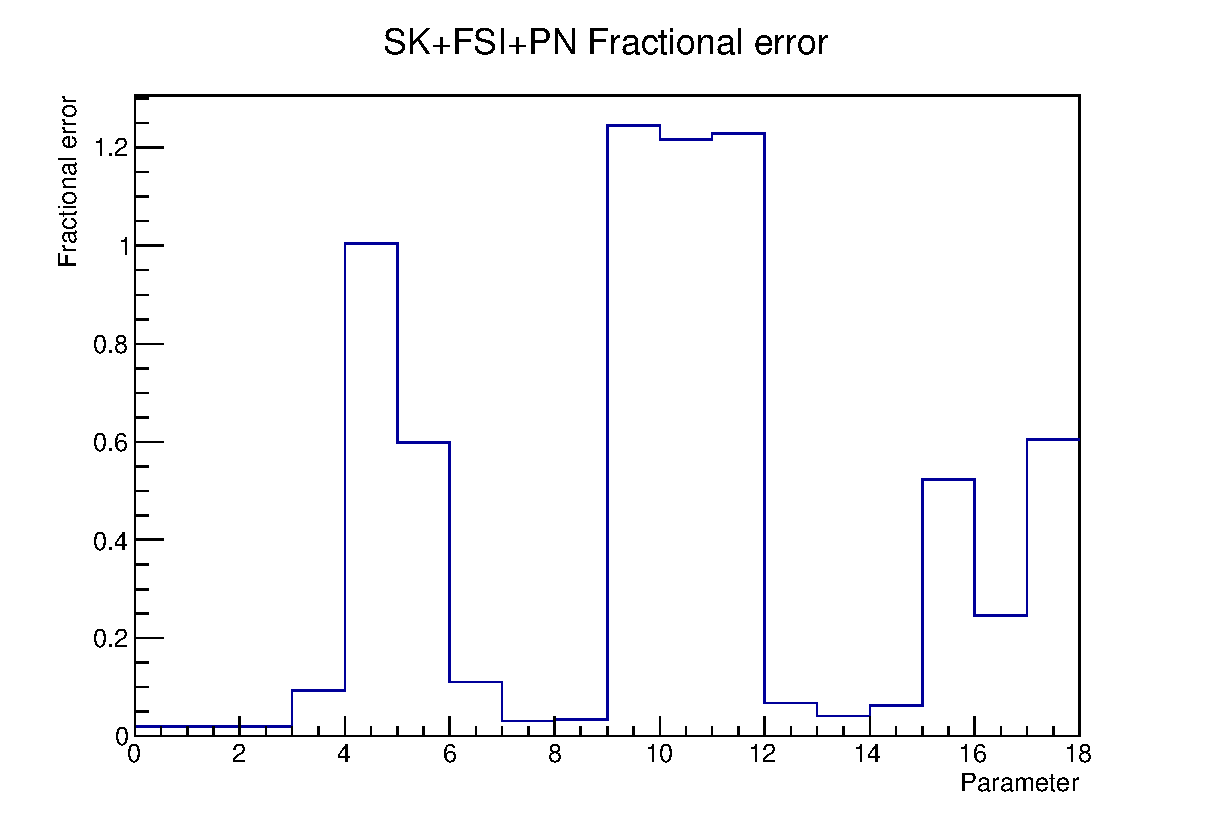
\includegraphics[width=20pc]{./images/systematics/SKFSIPN_frac_error_final.eps}
\caption {
 Values of the fractional errors for each SK+FSI+PN systematic parameter.
}
\label{fig:skfsi_frac}
\end{figure*}
 \begin{figure*}[htb]
\center
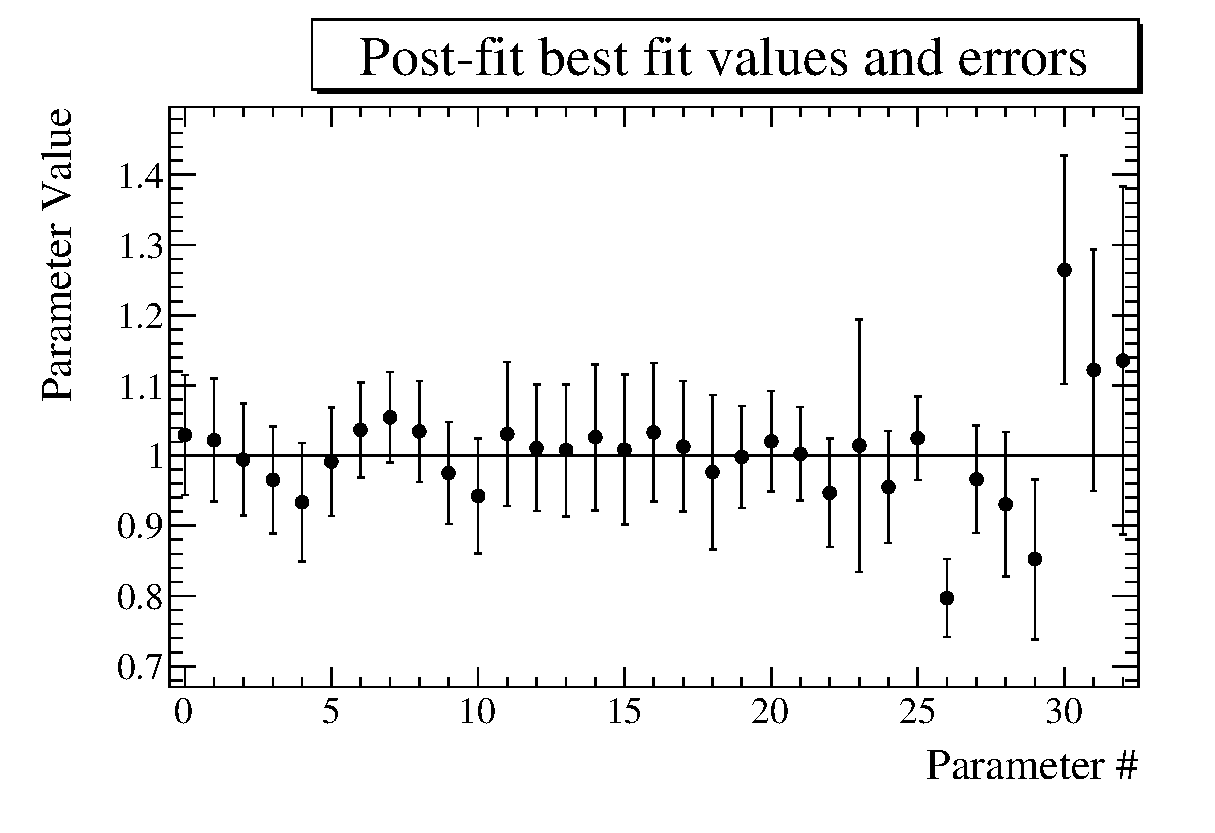
\includegraphics[width=20pc]{./images/systematics/BANFF_postfit_values_errors.eps}
\caption {
 Post-fit values and post-fit fractional errors for each BANFF systematic parameter.
}
\label{fig:banff}
\end{figure*}
\clearpage
{
\tiny
\begin{sideways}
\begin{minipage}{23cm}
{
\setlength{\arraycolsep}{1pt}
\begin{equation}
C^{banff} =\end{equation}
\begin{equation*}
\begin{blockarray}{c p{7pt}p{7pt}p{7pt}p{7pt}p{7pt}p{7pt}p{7pt}p{7pt}p{7pt}p{7pt}p{7pt}p{7pt}p{7pt}p{7pt}p{7pt}p{7pt}p{7pt}p{7pt}p{7pt}p{7pt}p{7pt}p{7pt}p{7pt}p{7pt}p{7pt}p{7pt}p{7pt}p{7pt}p{7pt}p{7pt}p{7pt}p{7pt}p{7pt}}
        & \begin{sideways} {\color{blue} $f_{0; t, r}^{banff}$} \end{sideways} & \begin{sideways} {\color{blue} $f_{1; t, r}^{banff}$} \end{sideways} & \begin{sideways} {\color{blue} $f_{2; t, r}^{banff}$} \end{sideways} & \begin{sideways} {\color{blue} $f_{3; t, r}^{banff}$} \end{sideways} & \begin{sideways} {\color{blue} $f_{4; t, r}^{banff}$} \end{sideways} & \begin{sideways} {\color{blue} $f_{5; t, r}^{banff}$} \end{sideways} & \begin{sideways} {\color{blue} $f_{6; t, r}^{banff}$} \end{sideways} & \begin{sideways} {\color{blue} $f_{7; t, r}^{banff}$} \end{sideways} & \begin{sideways} {\color{blue} $f_{8; t, r}^{banff}$} \end{sideways} & \begin{sideways} {\color{blue} $f_{9; t, r}^{banff}$} \end{sideways} & \begin{sideways} {\color{blue} $f_{10; t, r}^{banff}$} \end{sideways} & \begin{sideways} {\color{blue} $f_{11; t, r}^{banff}$} \end{sideways} & \begin{sideways} {\color{blue} $f_{12; t, r}^{banff}$} \end{sideways} & \begin{sideways} {\color{blue} $f_{13; t, r}^{banff}$} \end{sideways} & \begin{sideways} {\color{blue} $f_{14; t, r}^{banff}$} \end{sideways} & \begin{sideways} {\color{blue} $f_{15; t, r}^{banff}$} \end{sideways} & \begin{sideways} {\color{blue} $f_{16; t, r}^{banff}$} \end{sideways} & \begin{sideways} {\color{blue} $f_{17; t, r}^{banff}$} \end{sideways} & \begin{sideways} {\color{blue} $f_{18; t, r}^{banff}$} \end{sideways} & \begin{sideways} {\color{blue} $f_{19; t, r}^{banff}$} \end{sideways} & \begin{sideways} {\color{blue} $f_{20; t, r}^{banff}$} \end{sideways} & \begin{sideways} {\color{blue} $f_{21; t, r}^{banff}$} \end{sideways} & \begin{sideways} {\color{blue} $f_{22; t, r}^{banff}$} \end{sideways} & \begin{sideways} {\color{blue} $f_{23; t, r}^{banff}$} \end{sideways} & \begin{sideways} {\color{blue} $f_{24; t, r}^{banff}$} \end{sideways} & \begin{sideways} {\color{blue} $f_{25; t, r}^{banff}$} \end{sideways} & \begin{sideways} {\color{blue} $f_{26; t, r}^{banff}$} \end{sideways} & \begin{sideways} {\color{blue} $f_{27; t, r}^{banff}$} \end{sideways} & \begin{sideways} {\color{blue} $f_{28; t, r}^{banff}$} \end{sideways} & \begin{sideways} {\color{blue} $f_{29; t, r}^{banff}$} \end{sideways} & \begin{sideways} {\color{blue} $f_{30; t, r}^{banff}$} \end{sideways} & \begin{sideways} {\color{blue} $f_{31; t, r}^{banff}$} \end{sideways} & \begin{sideways} {\color{blue} $f_{32; t, r}^{banff}$} \end{sideways} \\ 
\begin{block}{c(p{7pt}p{7pt}p{7pt}p{7pt}p{7pt}p{7pt}p{7pt}p{7pt}p{7pt}p{7pt}p{7pt}p{7pt}p{7pt}p{7pt}p{7pt}p{7pt}p{7pt}p{7pt}p{7pt}p{7pt}p{7pt}p{7pt}p{7pt}p{7pt}p{7pt}p{7pt}p{7pt}p{7pt}p{7pt}p{7pt}p{7pt}p{7pt}p{7pt}@{\hspace*{1pt}})}
{\color{blue} f_{0; t, r}^{banff}}  \vspace{0.04cm} & {\color{red} 0.007} &      0.007 &      0.006 &      0.005 &      0.004 &      0.004 &      0.004 &      0.003 &      0.002 &      0.002 &      0.001 &      0.008 &      0.006 &      0.005 &      0.005 &      0.003 &      0.007 &      0.006 &      0.006 &      0.005 &      0.003 &      0.002 &      0.001 &      0.006 &      0.002 &     -0.001 &     -0.000 &     -0.004 &     -0.002 &     -0.001 &     -0.005 &     -0.002 &     -0.004 \\ 
{\color{blue} f_{1; t, r}^{banff}}  \vspace{0.04cm} &      0.007 & {\color{red} 0.008} &      0.007 &      0.005 &      0.005 &      0.005 &      0.004 &      0.003 &      0.002 &      0.002 &      0.001 &      0.006 &      0.005 &      0.004 &      0.004 &      0.002 &      0.006 &      0.007 &      0.006 &      0.005 &      0.003 &      0.002 &      0.001 &      0.005 &      0.002 &     -0.001 &     -0.000 &     -0.005 &     -0.002 &     -0.001 &     -0.006 &     -0.001 &     -0.004 \\ 
{\color{blue} f_{2; t, r}^{banff}}  \vspace{0.04cm} &      0.006 &      0.007 & {\color{red} 0.006} &      0.006 &      0.005 &      0.004 &      0.004 &      0.003 &      0.002 &      0.002 &      0.001 &      0.005 &      0.005 &      0.004 &      0.004 &      0.002 &      0.005 &      0.006 &      0.006 &      0.004 &      0.003 &      0.002 &      0.001 &      0.004 &      0.002 &     -0.001 &     -0.000 &     -0.005 &     -0.003 &     -0.001 &     -0.005 &     -0.001 &     -0.004 \\ 
{\color{blue} f_{3; t, r}^{banff}}  \vspace{0.04cm} &      0.005 &      0.005 &      0.006 & {\color{red} 0.006} &      0.005 &      0.005 &      0.004 &      0.003 &      0.002 &      0.002 &      0.001 &      0.005 &      0.005 &      0.005 &      0.004 &      0.002 &      0.005 &      0.005 &      0.005 &      0.004 &      0.003 &      0.002 &      0.001 &      0.004 &      0.002 &     -0.001 &     -0.000 &     -0.005 &     -0.003 &     -0.001 &     -0.006 &     -0.001 &     -0.004 \\ 
{\color{blue} f_{4; t, r}^{banff}}  \vspace{0.04cm} &      0.004 &      0.005 &      0.005 &      0.005 & {\color{red} 0.007} &      0.006 &      0.004 &      0.003 &      0.002 &      0.002 &      0.001 &      0.004 &      0.004 &      0.004 &      0.003 &      0.001 &      0.005 &      0.004 &      0.005 &      0.004 &      0.002 &      0.002 &      0.001 &      0.004 &      0.001 &     -0.001 &     -0.000 &     -0.005 &     -0.002 &     -0.001 &     -0.007 &     -0.001 &     -0.005 \\ 
{\color{blue} f_{5; t, r}^{banff}}  \vspace{0.04cm} &      0.004 &      0.005 &      0.004 &      0.005 &      0.006 & {\color{red} 0.006} &      0.005 &      0.003 &      0.002 &      0.002 &      0.001 &      0.005 &      0.005 &      0.005 &      0.004 &      0.002 &      0.005 &      0.005 &      0.004 &      0.004 &      0.003 &      0.002 &      0.001 &      0.004 &      0.001 &     -0.000 &     -0.000 &     -0.004 &     -0.003 &     -0.001 &     -0.007 &     -0.001 &     -0.005 \\ 
{\color{blue} f_{6; t, r}^{banff}}  \vspace{0.04cm} &      0.004 &      0.004 &      0.004 &      0.004 &      0.004 &      0.005 & {\color{red} 0.005} &      0.003 &      0.002 &      0.002 &      0.002 &      0.005 &      0.005 &      0.004 &      0.005 &      0.003 &      0.004 &      0.004 &      0.004 &      0.003 &      0.003 &      0.002 &      0.002 &      0.004 &      0.002 &     -0.000 &     -0.000 &     -0.003 &     -0.003 &     -0.001 &     -0.006 &     -0.002 &     -0.004 \\ 
{\color{blue} f_{7; t, r}^{banff}}  \vspace{0.04cm} &      0.003 &      0.003 &      0.003 &      0.003 &      0.003 &      0.003 &      0.003 & {\color{red} 0.004} &      0.003 &      0.002 &      0.001 &      0.004 &      0.003 &      0.003 &      0.003 &      0.001 &      0.003 &      0.003 &      0.003 &      0.003 &      0.003 &      0.003 &      0.001 &      0.003 &      0.002 &     -0.000 &     -0.000 &     -0.002 &     -0.002 &     -0.001 &     -0.003 &     -0.003 &     -0.002 \\ 
{\color{blue} f_{8; t, r}^{banff}}  \vspace{0.04cm} &      0.002 &      0.002 &      0.002 &      0.002 &      0.002 &      0.002 &      0.002 &      0.003 & {\color{red} 0.005} &      0.004 &      0.003 &      0.002 &      0.002 &      0.002 &      0.002 &      0.002 &      0.001 &      0.003 &      0.003 &      0.003 &      0.004 &      0.004 &      0.003 &      0.002 &      0.003 &     -0.000 &     -0.000 &     -0.002 &     -0.001 &     -0.002 &     -0.002 &     -0.005 &     -0.001 \\ 
{\color{blue} f_{9; t, r}^{banff}}  \vspace{0.04cm} &      0.002 &      0.002 &      0.002 &      0.002 &      0.002 &      0.002 &      0.002 &      0.002 &      0.004 & {\color{red} 0.005} &      0.005 &      0.002 &      0.002 &      0.002 &      0.003 &      0.004 &      0.001 &      0.001 &      0.001 &      0.002 &      0.003 &      0.004 &      0.005 &      0.000 &      0.004 &     -0.000 &      0.000 &     -0.001 &     -0.000 &     -0.002 &     -0.001 &     -0.006 &     -0.001 \\ 
{\color{blue} f_{10; t, r}^{banff}}  \vspace{0.04cm} &      0.001 &      0.001 &      0.001 &      0.001 &      0.001 &      0.001 &      0.002 &      0.001 &      0.003 &      0.005 & {\color{red} 0.007} &      0.001 &      0.002 &      0.001 &      0.003 &      0.005 &      0.001 &      0.001 &      0.002 &      0.002 &      0.003 &      0.004 &      0.006 &      0.002 &      0.005 &      0.000 &      0.000 &     -0.001 &      0.000 &     -0.002 &     -0.001 &     -0.005 &     -0.001 \\ 
{\color{blue} f_{11; t, r}^{banff}}  \vspace{0.04cm} &      0.008 &      0.006 &      0.005 &      0.005 &      0.004 &      0.005 &      0.005 &      0.004 &      0.002 &      0.002 &      0.001 & {\color{red} 0.010} &      0.008 &      0.008 &      0.007 &      0.004 &      0.008 &      0.007 &      0.006 &      0.005 &      0.004 &      0.002 &      0.002 &      0.007 &      0.003 &     -0.001 &     -0.000 &     -0.004 &     -0.003 &     -0.000 &     -0.006 &     -0.001 &     -0.004 \\ 
{\color{blue} f_{12; t, r}^{banff}}  \vspace{0.04cm} &      0.006 &      0.005 &      0.005 &      0.005 &      0.004 &      0.005 &      0.005 &      0.003 &      0.002 &      0.002 &      0.002 &      0.008 & {\color{red} 0.008} &      0.008 &      0.007 &      0.004 &      0.007 &      0.006 &      0.005 &      0.005 &      0.003 &      0.002 &      0.002 &      0.007 &      0.003 &     -0.001 &     -0.000 &     -0.004 &     -0.003 &     -0.001 &     -0.006 &     -0.001 &     -0.004 \\ 
{\color{blue} f_{13; t, r}^{banff}}  \vspace{0.04cm} &      0.005 &      0.004 &      0.004 &      0.005 &      0.004 &      0.005 &      0.004 &      0.003 &      0.002 &      0.002 &      0.001 &      0.008 &      0.008 & {\color{red} 0.009} &      0.007 &      0.004 &      0.007 &      0.006 &      0.005 &      0.005 &      0.003 &      0.002 &      0.002 &      0.008 &      0.003 &     -0.001 &     -0.000 &     -0.004 &     -0.003 &     -0.001 &     -0.006 &     -0.001 &     -0.004 \\ 
{\color{blue} f_{14; t, r}^{banff}}  \vspace{0.04cm} &      0.005 &      0.004 &      0.004 &      0.004 &      0.003 &      0.004 &      0.005 &      0.003 &      0.002 &      0.003 &      0.003 &      0.007 &      0.007 &      0.007 & {\color{red} 0.011} &      0.009 &      0.004 &      0.005 &      0.006 &      0.004 &      0.004 &      0.003 &      0.003 &      0.007 &      0.003 &     -0.000 &     -0.000 &     -0.003 &     -0.003 &     -0.000 &     -0.005 &     -0.002 &     -0.004 \\ 
{\color{blue} f_{15; t, r}^{banff}}  \vspace{0.04cm} &      0.003 &      0.002 &      0.002 &      0.002 &      0.001 &      0.002 &      0.003 &      0.001 &      0.002 &      0.004 &      0.005 &      0.004 &      0.004 &      0.004 &      0.009 & {\color{red} 0.011} &      0.002 &      0.002 &      0.004 &      0.002 &      0.003 &      0.003 &      0.004 &      0.004 &      0.004 &     -0.000 &     -0.000 &     -0.001 &     -0.002 &     -0.001 &     -0.002 &     -0.003 &     -0.002 \\ 
{\color{blue} f_{16; t, r}^{banff}}  \vspace{0.04cm} &      0.007 &      0.006 &      0.005 &      0.005 &      0.005 &      0.005 &      0.004 &      0.003 &      0.001 &      0.001 &      0.001 &      0.008 &      0.007 &      0.007 &      0.004 &      0.002 & {\color{red} 0.010} &      0.006 &      0.005 &      0.006 &      0.003 &      0.002 &      0.001 &      0.009 &      0.002 &     -0.001 &     -0.000 &     -0.004 &     -0.003 &     -0.000 &     -0.006 &     -0.002 &     -0.004 \\ 
{\color{blue} f_{17; t, r}^{banff}}  \vspace{0.04cm} &      0.006 &      0.007 &      0.006 &      0.005 &      0.004 &      0.005 &      0.004 &      0.003 &      0.003 &      0.001 &      0.001 &      0.007 &      0.006 &      0.006 &      0.005 &      0.002 &      0.006 & {\color{red} 0.009} &      0.006 &      0.005 &      0.004 &      0.002 &      0.001 &      0.009 &      0.003 &     -0.001 &     -0.000 &     -0.004 &     -0.002 &     -0.001 &     -0.006 &     -0.001 &     -0.004 \\ 
{\color{blue} f_{18; t, r}^{banff}}  \vspace{0.04cm} &      0.006 &      0.006 &      0.006 &      0.005 &      0.005 &      0.004 &      0.004 &      0.003 &      0.003 &      0.001 &      0.002 &      0.006 &      0.005 &      0.005 &      0.006 &      0.004 &      0.005 &      0.006 & {\color{red} 0.012} &      0.006 &      0.005 &      0.003 &      0.002 &      0.008 &      0.002 &     -0.001 &     -0.000 &     -0.005 &     -0.003 &     -0.001 &     -0.006 &     -0.001 &     -0.004 \\ 
{\color{blue} f_{19; t, r}^{banff}}  \vspace{0.04cm} &      0.005 &      0.005 &      0.004 &      0.004 &      0.004 &      0.004 &      0.003 &      0.003 &      0.003 &      0.002 &      0.002 &      0.005 &      0.005 &      0.005 &      0.004 &      0.002 &      0.006 &      0.005 &      0.006 & {\color{red} 0.005} &      0.004 &      0.003 &      0.002 &      0.009 &      0.003 &     -0.001 &     -0.000 &     -0.004 &     -0.002 &     -0.001 &     -0.005 &     -0.002 &     -0.004 \\ 
{\color{blue} f_{20; t, r}^{banff}}  \vspace{0.04cm} &      0.003 &      0.003 &      0.003 &      0.003 &      0.002 &      0.003 &      0.003 &      0.003 &      0.004 &      0.003 &      0.003 &      0.004 &      0.003 &      0.003 &      0.004 &      0.003 &      0.003 &      0.004 &      0.005 &      0.004 & {\color{red} 0.005} &      0.004 &      0.003 &      0.007 &      0.004 &     -0.000 &     -0.000 &     -0.002 &     -0.001 &     -0.002 &     -0.003 &     -0.004 &     -0.002 \\ 
{\color{blue} f_{21; t, r}^{banff}}  \vspace{0.04cm} &      0.002 &      0.002 &      0.002 &      0.002 &      0.002 &      0.002 &      0.002 &      0.003 &      0.004 &      0.004 &      0.004 &      0.002 &      0.002 &      0.002 &      0.003 &      0.003 &      0.002 &      0.002 &      0.003 &      0.003 &      0.004 & {\color{red} 0.004} &      0.004 &      0.003 &      0.004 &     -0.000 &     -0.000 &     -0.002 &     -0.001 &     -0.002 &     -0.002 &     -0.005 &     -0.001 \\ 
{\color{blue} f_{22; t, r}^{banff}}  \vspace{0.04cm} &      0.001 &      0.001 &      0.001 &      0.001 &      0.001 &      0.001 &      0.002 &      0.001 &      0.003 &      0.005 &      0.006 &      0.002 &      0.002 &      0.002 &      0.003 &      0.004 &      0.001 &      0.001 &      0.002 &      0.002 &      0.003 &      0.004 & {\color{red} 0.006} &      0.002 &      0.005 &     -0.000 &      0.000 &     -0.001 &     -0.000 &     -0.002 &     -0.001 &     -0.005 &     -0.001 \\ 
{\color{blue} f_{23; t, r}^{banff}}  \vspace{0.04cm} &      0.006 &      0.005 &      0.004 &      0.004 &      0.004 &      0.004 &      0.004 &      0.003 &      0.002 &      0.000 &      0.002 &      0.007 &      0.007 &      0.008 &      0.007 &      0.004 &      0.009 &      0.009 &      0.008 &      0.009 &      0.007 &      0.003 &      0.002 & {\color{red} 0.032} &      0.006 &     -0.001 &     -0.000 &     -0.003 &     -0.002 &     -0.000 &     -0.005 &     -0.001 &     -0.004 \\ 
{\color{blue} f_{24; t, r}^{banff}}  \vspace{0.04cm} &      0.002 &      0.002 &      0.002 &      0.002 &      0.001 &      0.001 &      0.002 &      0.002 &      0.003 &      0.004 &      0.005 &      0.003 &      0.003 &      0.003 &      0.003 &      0.004 &      0.002 &      0.003 &      0.002 &      0.003 &      0.004 &      0.004 &      0.005 &      0.006 & {\color{red} 0.006} &     -0.000 &      0.000 &     -0.001 &      0.000 &     -0.002 &     -0.001 &     -0.004 &     -0.000 \\ 
{\color{blue} f_{25; t, r}^{banff}}  \vspace{0.04cm} &     -0.001 &     -0.001 &     -0.001 &     -0.001 &     -0.001 &     -0.000 &     -0.000 &     -0.000 &     -0.000 &     -0.000 &      0.000 &     -0.001 &     -0.001 &     -0.001 &     -0.000 &     -0.000 &     -0.001 &     -0.001 &     -0.001 &     -0.001 &     -0.000 &     -0.000 &     -0.000 &     -0.001 &     -0.000 & {\color{red} 0.004} &     -0.001 &     -0.001 &     -0.002 &     -0.002 &      0.001 &      0.002 &      0.001 \\ 
{\color{blue} f_{26; t, r}^{banff}}  \vspace{0.04cm} &     -0.000 &     -0.000 &     -0.000 &     -0.000 &     -0.000 &     -0.000 &     -0.000 &     -0.000 &     -0.000 &      0.000 &      0.000 &     -0.000 &     -0.000 &     -0.000 &     -0.000 &     -0.000 &     -0.000 &     -0.000 &     -0.000 &     -0.000 &     -0.000 &     -0.000 &      0.000 &     -0.000 &      0.000 &     -0.001 & {\color{red} 0.003} &      0.000 &      0.000 &      0.000 &     -0.004 &     -0.004 &     -0.003 \\ 
{\color{blue} f_{27; t, r}^{banff}}  \vspace{0.04cm} &     -0.004 &     -0.005 &     -0.005 &     -0.005 &     -0.005 &     -0.004 &     -0.003 &     -0.002 &     -0.002 &     -0.001 &     -0.001 &     -0.004 &     -0.004 &     -0.004 &     -0.003 &     -0.001 &     -0.004 &     -0.004 &     -0.005 &     -0.004 &     -0.002 &     -0.002 &     -0.001 &     -0.003 &     -0.001 &     -0.001 &      0.000 & {\color{red} 0.006} &      0.004 &      0.002 &      0.005 &      0.000 &      0.003 \\ 
{\color{blue} f_{28; t, r}^{banff}}  \vspace{0.04cm} &     -0.002 &     -0.002 &     -0.003 &     -0.003 &     -0.002 &     -0.003 &     -0.003 &     -0.002 &     -0.001 &     -0.000 &      0.000 &     -0.003 &     -0.003 &     -0.003 &     -0.003 &     -0.002 &     -0.003 &     -0.002 &     -0.003 &     -0.002 &     -0.001 &     -0.001 &     -0.000 &     -0.002 &      0.000 &     -0.002 &      0.000 &      0.004 & {\color{red} 0.011} &      0.005 &      0.001 &     -0.005 &      0.001 \\ 
{\color{blue} f_{29; t, r}^{banff}}  \vspace{0.04cm} &     -0.001 &     -0.001 &     -0.001 &     -0.001 &     -0.001 &     -0.001 &     -0.001 &     -0.001 &     -0.002 &     -0.002 &     -0.002 &     -0.000 &     -0.001 &     -0.001 &     -0.000 &     -0.001 &     -0.000 &     -0.001 &     -0.001 &     -0.001 &     -0.002 &     -0.002 &     -0.002 &     -0.000 &     -0.002 &     -0.002 &      0.000 &      0.002 &      0.005 & {\color{red} 0.013} &     -0.003 &     -0.006 &     -0.002 \\ 
{\color{blue} f_{30; t, r}^{banff}}  \vspace{0.04cm} &     -0.005 &     -0.006 &     -0.005 &     -0.006 &     -0.007 &     -0.007 &     -0.006 &     -0.003 &     -0.002 &     -0.001 &     -0.001 &     -0.006 &     -0.006 &     -0.006 &     -0.005 &     -0.002 &     -0.006 &     -0.006 &     -0.006 &     -0.005 &     -0.003 &     -0.002 &     -0.001 &     -0.005 &     -0.001 &      0.001 &     -0.004 &      0.005 &      0.001 &     -0.003 & {\color{red} 0.027} &      0.011 &      0.020 \\ 
{\color{blue} f_{31; t, r}^{banff}}  \vspace{0.04cm} &     -0.002 &     -0.001 &     -0.001 &     -0.001 &     -0.001 &     -0.001 &     -0.002 &     -0.003 &     -0.005 &     -0.006 &     -0.005 &     -0.001 &     -0.001 &     -0.001 &     -0.002 &     -0.003 &     -0.002 &     -0.001 &     -0.001 &     -0.002 &     -0.004 &     -0.005 &     -0.005 &     -0.001 &     -0.004 &      0.002 &     -0.004 &      0.000 &     -0.005 &     -0.006 &      0.011 & {\color{red} 0.029} &      0.009 \\ 
{\color{blue} f_{32; t, r}^{banff}}  \vspace{0.04cm} &     -0.004 &     -0.004 &     -0.004 &     -0.004 &     -0.005 &     -0.005 &     -0.004 &     -0.002 &     -0.001 &     -0.001 &     -0.001 &     -0.004 &     -0.004 &     -0.004 &     -0.004 &     -0.002 &     -0.004 &     -0.004 &     -0.004 &     -0.004 &     -0.002 &     -0.001 &     -0.001 &     -0.004 &     -0.000 &      0.001 &     -0.003 &      0.003 &      0.001 &     -0.002 &      0.020 &      0.009 & {\color{red} 0.061} \\ 
\end{block}
\label{eq:Cbanff}
\end{blockarray}
\end{equation*}
}
\end{minipage}
\end{sideways}
\normalsize
}





%
% ...............................................................................
% Table summarizing which systematics are applied to which sample
%

\begin{table}[htbp]
\center
\begin{tabular}{|p{1cm}|p{3cm}|p{5.75cm}|p{0.75cm}|p{0.75cm}|p{0.75cm}|p{0.75cm}|p{0.75cm}|}
\hline 
 & & & \multicolumn{2}{c|}{Stand-alone} & \multicolumn{2}{c|}{Joint OA} & \\
Type & Systematics & Comment & $1R_{\mu}$ & $1R_{e}$ & $1R_{\mu}$ & $1R_{e}$ & $N_{syst}$ \\
\hline 
\hline
  \multirow{6}{*} { \begin{sideways} BANFF \end{sideways} } 
       & $f_{0; t, r}^{banff}$ - $f_{24; t, r}^{banff}$          
          & $\nu_{\mu}$  flux &  11 &  11  &  11 & 11 & 25 \\
 
&    &  $\bar{\nu_{\mu}}$  flux &  5 &  2  &  5 & 5 &  \\
&    &  ${\nu_{e}}$  flux &  -- &  7  &  7 &  7 &\\
&    &  $\bar{\nu_{e}}$  flux &  -- &  2  &  2 & 2 & \\
  \cline{2-8}
       & $f_{25; t, r}^{banff}$ 
          & CCQE axial mass                  &  {\ck} &  {\ck} & \ck & \ck & 8 \\
       & $f_{26; t, r}^{banff}$ 
          & resonance-production axial mass  &  {\ck} &  {\ck} & \ck & \ck & \\
       & $f_{27; t, r}^{banff}$ - $f_{29; t, r}^{banff}$  
          & CCQE normalization            &  3 &  1 & 3 & 3 & \\
       & $f_{30; t, r}^{banff}$ - $f_{31; t, r}^{banff}$ 
          & CC1$\pi$ normalization        &  2 &  1 & 2 &  2 & \\
       & $f_{32; t, r}^{banff}$ 
          & NC1$\pi^{0}$                  &   --               &  \ck               & -- & \ck & \\
\hline
  \multirow{12}{*} {  \begin{sideways} Uncorrelated cross-section \end{sideways} } 
       & $f_{pF; t, r}$ 
          & Fermi momentum           &  {\ck} &  {\ck} & \ck & \ck &12 \\
       & $f_{bindE; t, r}$ 
         & Binding energy            &  {\ck} &  -- & \ck & \ck & \\
       & $f_{SF; t, r}$
         & Nuclear modeling          &  {\ck} &  {\ck} & \ck &  \ck &  \\
       & $f_{Wshape; t, r}$
         & Shape of the $\pi$ momentum distribution    &  {\ck} &  {\ck} & \ck & \ck & \\
       & $f_{\pi-less\Delta; t, r}$
         & $\pi$-less $\Delta$ decay    &  {\ck} &  {\ck} & \ck &  \ck & \\
       & $f_{CCothShape; t, r}$
         & CC other shape               &  {\ck} &  {\ck} & \ck & \ck & \\
       & $f_{CCcoh; t}$
         & CC coherent cross-section    & {\ck} &  {\ck} & \ck & \ck &  \\
       & $f_{NC1\pi^\pm; t}$
         & NC1$\pi^{\pm}$ cross-section & \ck & -- & \ck & -- &\\
       & $f_{NCcoh; t}$
         & NC coherent cross-section    & -- & \ck & -- & \ck & \\
       & $f_{NCoth; t}$
         & NC other cross-section       & {\ck} &  {\ck} & \ck & \ck & \\
       & $f_{CC\nu_e; t}$
         & $\sigma_{\nu_{e}}$/ $\sigma_{\nu_{\mu}}$ ratio & {\ck} &  {\ck} & \ck & \ck & \\
       & $f_{CC\bar{\nu}; t}$
         & $\sigma_{\bar{\nu}}$/ $\sigma_{\nu}$ ratio      & {\ck} &  -- & \ck & \ck & \\
\hline 
\hline
   \multirow{3}{*} { \begin{sideways} SK + FSI\end{sideways} } 
      & $f_{E; r}^{SK}$  
          & Reconstructed energy scale & {\ck}  &  {\ck}  & \ck & \ck & 1 \\
   \cline{2-8}
      & $f_{0; r}^{SK+FSI}$-$f_{5; r}^{SK+FSI}$ 
          &  $1R_{\mu}$ efficiencies  & \ck & -- &  \ck & --& 6  \\
   \cline{2-8}
       & $f_{6; r}^{SK+FSI}$-$f_{17; r}^{SK+FSI}$ 
          &  $1R_{e}$ efficiencies  & -- & \ck &  -- & \ck & 12 \\
 \hline 
\hline
\bf Total &  &  & \bf 41 & \bf 49 & \multicolumn{2}{|c|}{\bf 64} & \\
\hline
\end{tabular}
\caption{
  List of all systematic parameters included in the joint oscillation analysis.
  A \ck symbol indicates whether the systematic parameter is applied on the single $\mu$-like ring 
  and single e-like ring MC templates.
}
\label{tab:apply_syst_to_samples}
\end{table}




% .................
\clearpage
% ........................................
%
% table showing which systematics are applied to which 1Rmu modes
%

{
\setlength{\tabcolsep}{2pt}
\renewcommand{\arraystretch}{1.5}
\begin{table}
\scriptsize
\centering
\begin{tabular}{| c || c | c | c | c | c | c || c | c | c | c | c | c || c | c | c | c | c | c || c | c | c | c | c | c || c | c | c | c || c | c | c | c || c | c | c | c |}
\hline
                       & \begin{sideways}   $\nu_{\mu}$ CCQE                   \end{sideways}  &   
                         \begin{sideways}   $\nu_{\mu}$ CC1$\pi$               \end{sideways}  &   
                         \begin{sideways}   $\nu_{\mu}$ CC coherent            \end{sideways}  &   
                         \begin{sideways}   $\nu_{\mu}$ CC other               \end{sideways}  &   
                         \begin{sideways}   $\nu_{\mu}$ NC1$\pi^{\pm}$         \end{sideways}  &  
                         \begin{sideways}   $\nu_{\mu}$ NC other               \end{sideways}  &   
                         \begin{sideways}   $\bar{\nu_{\mu}}$ CCQE             \end{sideways}  &  
                         \begin{sideways}   $\bar{\nu_{\mu}}$ CC1$\pi$         \end{sideways}  &  
                         \begin{sideways}   $\bar{\nu_{\mu}}$ CC coherent      \end{sideways}  &  
                         \begin{sideways}   $\bar{\nu_{\mu}}$ CC other         \end{sideways}  &  
                         \begin{sideways}   $\bar{\nu_{\mu}}$ NC1$\pi^{\pm}$   \end{sideways}  &   
                         \begin{sideways}   $\bar{\nu_{\mu}}$ NC other         \end{sideways}  &   
                         \begin{sideways}   $\nu_{e}$ CCQE                     \end{sideways}  &   
                         \begin{sideways}   $\nu_{e}$ CC1$\pi$                 \end{sideways}  &   
                         \begin{sideways}   $\nu_{e}$ CC coherent              \end{sideways}  &  
                         \begin{sideways}   $\nu_{e}$ CC other                 \end{sideways}  &   
                         \begin{sideways}   $\nu_{e}$ NC1$\pi^{\pm}$           \end{sideways}  &   
                         \begin{sideways}   $\nu_{e}$ NC other                 \end{sideways}  &  
                         \begin{sideways}   $\bar{\nu_{e}}$ CCQE               \end{sideways}  &   
                         \begin{sideways}   $\bar{\nu_{e}}$ CC1$\pi$           \end{sideways}  &   
                         \begin{sideways}   $\bar{\nu_{e}}$ CC coherent        \end{sideways}  &   
                         \begin{sideways}   $\bar{\nu_{e}}$ CC other           \end{sideways}  &  
                         \begin{sideways}   $\bar{\nu_{e}}$ NC1$\pi^{\pm}$     \end{sideways}  & 
                         \begin{sideways}   $\bar{\nu_{e}}$ NC other           \end{sideways}  &   
                         \begin{sideways}   Osc-$\nu_{e}$ CCQE                 \end{sideways}  &   
                         \begin{sideways}   Osc-$\nu_{e}$ CC1$\pi$             \end{sideways}  &   
                         \begin{sideways}   Osc-$\nu_{e}$ CC coherent          \end{sideways}  &   
                         \begin{sideways}   Osc-$\nu_{e}$ CC other             \end{sideways}  &
                           \begin{sideways}   Osc-$\nu_{\mu}$ CCQE                 \end{sideways}  &   
                         \begin{sideways}   Osc-$\nu_{\mu}$ CC1$\pi$             \end{sideways}  &   
                         \begin{sideways}   Osc-$\nu_{\mu}$ CC coherent          \end{sideways}  &   
                         \begin{sideways}   Osc-$\nu_{\mu}$ CC other             \end{sideways}  &
                           \begin{sideways}   Osc-$\bar{\nu_{e}}$ CCQE                 \end{sideways}  &   
                         \begin{sideways}   Osc-$\bar{\nu_{e}}$ CC1$\pi$             \end{sideways}  &   
                         \begin{sideways}   Osc-$\bar{\nu_{e}}$ CC coherent          \end{sideways}  &   
                         \begin{sideways}   Osc-$\bar{\nu_{e}}$ CC other             \end{sideways}  \\
\hline
 $f_{E; r}^{SK}$             & \ck & \ck & \ck & \ck & \ck & \ck & \ck & \ck & \ck & \ck & \ck & \ck & \ck & \ck & \ck & \ck & \ck & \ck & \ck & \ck & \ck & \ck & \ck & \ck & \ck & \ck & \ck & \ck  & \ck & \ck & \ck & \ck & \ck & \ck & \ck & \ck \\
\hline
 $f_{0; t, r}^{banff}$ -
 $f_{10; t, r}^{banff}$      & \ck & \ck & \ck & \ck & \ck & \ck &     &     &     &     &     &     &     &     &     &     &     &     &     &     &     &     &     &   & \ck & \ck & \ck & \ck &   &    &     &     &  & & &    \\ 
\hline
 $f_{11; t, r}^{banff}$ -   
 $f_{15; t, r}^{banff}$      &     &     &     &     &     &     & \ck & \ck & \ck & \ck & \ck & \ck &     &     &     &     &     &     &     &     &     &     &     &     &     &     &     &    & & & & &\ck & \ck & \ck & \ck   \\
\hline
 $f_{16; t, r}^{banff}$ -   
 $f_{22; t, r}^{banff}$      &     &     &     &     &     &     &     &     &     &     &     &     & \ck & \ck & \ck & \ck & \ck & \ck &     &     &     &     &     &     &     &     &     &    & \ck & \ck & \ck & \ck  & & & & \\
\hline
 $f_{23; t, r}^{banff}$ -   
 $f_{24; t, r}^{banff}$      &     &     &     &     &     &     &     &     &     &     &     &     &     &     &     &     &     &   & \ck & \ck & \ck & \ck & \ck & \ck &    &     &     &   & & & & & & & &    \\
\hline
 $f_{25; t, r}^{banff}$      & \ck &     &     &     &     &     & \ck &     &     &     &     &     & \ck &     &     &     &     &     & \ck &     &     &     &     &     & \ck &     &     &  & \ck &     &     &  & \ck &     &     &       \\
\hline
 $f_{26; t, r}^{banff}$      &     & \ck &     & \ck & \ck & \ck &     & \ck &     & \ck & \ck & \ck &     & \ck &     & \ck & \ck & \ck &     & \ck &     & \ck & \ck & \ck &     &\ck  &     & \ck &     &\ck  &     & \ck &     &\ck  &     & \ck  \\
\hline
 $f_{27; t, r}^{banff}$      & \ck &     &     &     &     &     & \ck &     &     &     &     &     & \ck &     &     &     &     &     & \ck &     &     &     &     &     & \ck &     &     &  & \ck &     &     &  & \ck &     &     &       \\
\hline
 $f_{28; t, r}^{banff}$      & \ck &     &     &     &     &     & \ck &     &     &     &     &     & \ck &     &     &     &     &     & \ck &     &     &     &     &     & \ck &     &     &  & \ck &     &     &  & \ck &     &     &       \\
\hline
 $f_{29; t, r}^{banff}$      & \ck &     &     &     &     &     & \ck &     &     &     &     &     & \ck &     &     &     &     &     & \ck &     &     &     &     &     & \ck &     &     &  & \ck &     &     &  & \ck &     &     &       \\
\hline
 $f_{30; t, r}^{banff}$      &     & \ck &     &     &     &     &     & \ck &     &     &     &     &     & \ck &     &     &     &     &     & \ck &     &     &     &     &     & \ck &     &      &     & \ck &     &       &     & \ck &     &      \\
\hline
 $f_{31; t, r}^{banff}$      &     & \ck &     &     &     &     &     & \ck &     &     &     &     &     & \ck &     &     &     &     &     & \ck &     &     &     &     &     & \ck &     &       &     & \ck &     &       &     & \ck &     &   \\
\hline
$f_{32; t, r}^{banff}$      &     &  &     &     &     &     &     &  &     &     &     &     &     &  &     &     &     &     &     &  &     &     &     &     &     &  &     &       &     &  &     &       &     &  &     &   \\
\hline
 $f_{pF; t, r}$               & \ck &     &     &     &     &     & \ck &     &     &     &     &     & \ck &     &     &     &     &     & \ck &     &     &     &     &     & \ck &     &     &  & \ck &     &     &  & \ck &     &     &       \\
\hline
 $f_{SF; t, r}$               & \ck &     &     &     &     &     & \ck &     &     &     &     &     & \ck &     &     &     &     &     & \ck &     &     &     &     &     & \ck &     &     &  & \ck &     &     &  & \ck &     &     &       \\
\hline
 $f_{bindE; t, r}$           & \ck &     &     &     &     &     & \ck &     &     &     &     &     & \ck &     &     &     &     &     & \ck &     &     &     &     &     & \ck &     &     &  & \ck &     &     &  & \ck &     &     &       \\
\hline
 $f_{\pi-less\Delta; t, r}$  &     &\ck  &     &     & \ck & \ck &     & \ck &     &     & \ck & \ck &     & \ck &     &     &\ck  &\ck  &     & \ck &     &     & \ck & \ck &     & \ck &     &     &     & \ck &     &     &     & \ck &     &      \\
\hline
 $f_{CCothShape; t, r}$      &     &     &     &\ck  &     &     &     &     &     & \ck &     &     &     &     &     & \ck &     &     &     &     &     & \ck &     &     &     &     &     & \ck&     &     &     & \ck &     &     &     & \ck  \\
\hline
 $f_{Wshape; t, r}$          &     &     &     &     & \ck & \ck &     &     &     &     &\ck  & \ck &     &     &     &     & \ck & \ck &     &     &     &     &\ck  & \ck &     &     &     &  &     &     &     &  &     &     &     &      \\
\hline
 $f_{CCcoh; t}$              &     &     & \ck &     &     &     &     &     & \ck &     &     &     &     &     & \ck &     &     &     &     &     & \ck &     &     &     &     &     & \ck &      &     &     & \ck &       &     &     & \ck &      \\
\hline
 $f_{NC1\pi^\pm; t}$         &     &     &     &     & \ck &     &     &     &     &     & \ck &     &     &     &     &     & \ck &     &     &     &     &     & \ck &     &     &     &     &    &     &     &     &    &     &     &     &      \\
\hline
 $f_{NCcoh; t}$  &     &  &     &     &     &     &     &  &     &     &     &     &     &  &     &     &     &     &     &  &     &     &     &     &     &  &     &       &     &  &     &       &     &  &     &   \\
\hline
 $f_{NCoth; t}$              &     &     &     &     &     & \ck &     &     &     &     &     & \ck &     &     &     &     &     & \ck &     &     &     &     &     &\ck  &     &     &     & &     &     &     & &     &     &     &      \\
\hline
 $f_{CC\nu_e; t}$            &     &     &     &     &     &     &     &     &     &     &     &     & \ck & \ck & \ck &\ck  &     &     &\ck  &\ck  & \ck & \ck &     &     & \ck & \ck & \ck & \ck &     &     &     &     & \ck & \ck & \ck & \ck\\
\hline
 $f_{CC\bar{\nu}; t}$        &     &     &     &     &     &     & \ck & \ck & \ck & \ck &     &     &     &     &     &     &     &     & \ck & \ck & \ck & \ck &     &     &     &     &     &  &     &     &     &     & \ck & \ck & \ck & \ck   \\
\hline
 $f _{0; r}^{SK+FSI}$      & \ck &     &     &     &     &     & \ck &     &     &     &     &     &     &     &     &     &     &     &     &     &     &     &     &     &     &     &     &    & \ck &     &     &     &     &     &     &    \\
\hline
 $f _{1; r}^{SK+FSI}$      & \ck &     &     &     &     &     & \ck &     &     &     &     &     &     &     &     &     &     &     &     &     &     &     &     &     &     &     &     &    & \ck &     &     &     &     &     &     &  \\
\hline
 $f _{2; r}^{SK+FSI}$      & \ck &     &     &     &     &     & \ck &     &     &     &     &     &     &     &     &     &     &     &     &     &     &     &     &     &     &     &     &    & \ck &     &     &     &     &     &     &      \\
\hline
 $f _{3; r}^{SK+FSI}$      &     & \ck & \ck & \ck &     &     &     & \ck & \ck & \ck &     &     &     &     &     &     &     &     &     &     &     &     &     &     &     &     &     &    &     & \ck & \ck & \ck  &     &     &     &   \\
\hline
 $f _{4; r}^{SK+FSI}$      &     &     &     &     &     &     &     &     &     &     &     &     & \ck & \ck & \ck & \ck &     &     & \ck & \ck & \ck & \ck &     &     & \ck & \ck & \ck & \ck  &     &     &     &  & \ck & \ck & \ck & \ck\\
\hline
 $f _{5; r}^{SK+FSI}$      &     &     &     &     & \ck & \ck &     &     &     &     & \ck & \ck &     &     &     &     & \ck & \ck &     &     &     &     & \ck & \ck &     &     &     & &     &     &     & &     &     &     &      \\
\hline
$f _{6; r}^{SK+FSI}$-$f _{17; r}^{SK+FSI}$ &     &  &     &     &     &     &     &  &     &     &     &     &     &  &     &     &     &     &     &  &     &     &     &     &     &  &     &       &     &  &     &       &     &  &     &   \\
\hline
\end{tabular}
\caption{
  A \ck symbol denotes that the given single $\mu$-like ring MC template is modified when the given systematic parameter is tweaked.
  The table lists all systematic parameters considered in this analysis (first column),
and all 36 MC templates used for constructing the single $\mu$-like ring event reconstructed energy spectrum p.d.f (first row).
}
\label{tab:apply_syst_to_1Rmu_templates}
\end{table}
}




\clearpage
% ........................................
%
% table showing which systematics are applied to which 1Re modes
%

{
\setlength{\tabcolsep}{2pt}
\renewcommand{\arraystretch}{1.4}
\begin{table}
\scriptsize
\centering
\begin{tabular}{| c || c | c | c | c | c | c | c || c | c | c | c | c | c | c || c | c | c | c | c | c | c || c | c | c | c | c | c | c || c | c | c | c || c | c | c | c || c | c | c | c |}
\hline
                       & \begin{sideways}   $\nu_{\mu}$ CCQE                   \end{sideways}  &   
                         \begin{sideways}   $\nu_{\mu}$ CC1$\pi$               \end{sideways}  &   
                         \begin{sideways}   $\nu_{\mu}$ CC coherent            \end{sideways}  &   
                         \begin{sideways}   $\nu_{\mu}$ CC other               \end{sideways}  &   
                         \begin{sideways}   $\nu_{\mu}$ NC1$\pi^{0}$           \end{sideways}  &  
                         \begin{sideways}   $\nu_{\mu}$ NC coherent            \end{sideways}  &  
                         \begin{sideways}   $\nu_{\mu}$ NC other               \end{sideways}  &   
                         \begin{sideways}   $\bar{\nu_{\mu}}$ CCQE             \end{sideways}  &  
                         \begin{sideways}   $\bar{\nu_{\mu}}$ CC1$\pi$         \end{sideways}  &  
                         \begin{sideways}   $\bar{\nu_{\mu}}$ CC coherent      \end{sideways}  &  
                         \begin{sideways}   $\bar{\nu_{\mu}}$ CC other         \end{sideways}  &  
                         \begin{sideways}   $\bar{\nu_{\mu}}$ NC1$\pi^{0}$     \end{sideways}  &   
                         \begin{sideways}   $\bar{\nu_{\mu}}$ NC coherent      \end{sideways}  &   
                         \begin{sideways}   $\bar{\nu_{\mu}}$ NC other         \end{sideways}  & 
                         \begin{sideways}   $\nu_{e}$ CCQE                     \end{sideways}  &   
                         \begin{sideways}   $\nu_{e}$ CC1$\pi$                 \end{sideways}  &   
                         \begin{sideways}   $\nu_{e}$ CC coherent              \end{sideways}  &  
                         \begin{sideways}   $\nu_{e}$ CC other                 \end{sideways}  &   
                         \begin{sideways}   $\nu_{e}$ NC1$\pi^{0}$             \end{sideways}  &   
                         \begin{sideways}   $\nu_{e}$ NC coherent              \end{sideways}  &   
                         \begin{sideways}   $\nu_{e}$ NC other                 \end{sideways}  &  
                         \begin{sideways}   $\bar{\nu_{e}}$ CCQE               \end{sideways}  &   
                         \begin{sideways}   $\bar{\nu_{e}}$ CC1$\pi$           \end{sideways}  &   
                         \begin{sideways}   $\bar{\nu_{e}}$ CC coherent        \end{sideways}  &   
                         \begin{sideways}   $\bar{\nu_{e}}$ CC other           \end{sideways}  &  
                         \begin{sideways}   $\bar{\nu_{e}}$ NC1$\pi^{0}$       \end{sideways}  & 
                         \begin{sideways}   $\bar{\nu_{e}}$ NC coherent        \end{sideways}  &   
                         \begin{sideways}   $\bar{\nu_{e}}$ NC other           \end{sideways}  &   
                         \begin{sideways}   Osc-$\nu_{e}$ CCQE                 \end{sideways}  &   
                         \begin{sideways}   Osc-$\nu_{e}$ CC1$\pi$             \end{sideways}  &   
                         \begin{sideways}   Osc-$\nu_{e}$ CC coherent          \end{sideways}  &   
                         \begin{sideways}   Osc-$\nu_{e}$ CC other             \end{sideways}  &
 			  \begin{sideways}   Osc-$\nu_{\mu}$ CCQE                 \end{sideways}  &   
                         \begin{sideways}   Osc-$\nu_{\mu}$ CC1$\pi$             \end{sideways}  &   
                         \begin{sideways}   Osc-$\nu_{\mu}$ CC coherent          \end{sideways}  &   
                         \begin{sideways}   Osc-$\nu_{\mu}$ CC other             \end{sideways}  &
                         \begin{sideways}   Osc-$\bar{\nu_{e}}$ CCQE                 \end{sideways}  &   
                         \begin{sideways}   Osc-$\bar{\nu_{e}}$ CC1$\pi$             \end{sideways}  &   
                         \begin{sideways}   Osc-$\bar{\nu_{e}}$ CC coherent          \end{sideways}  &   
                         \begin{sideways}   Osc-$\bar{\nu_{e}}$ CC other             \end{sideways}  \\
\hline
 $f_{E; r}^{SK}$             & \ck & \ck & \ck & \ck & \ck & \ck & \ck & \ck & \ck & \ck & \ck & \ck & \ck & \ck & \ck & \ck & \ck & \ck & \ck & \ck & \ck & \ck & \ck & \ck & \ck & \ck & \ck & \ck & \ck & \ck & \ck & \ck & \ck & \ck & \ck & \ck& \ck & \ck & \ck & \ck \\
\hline
  $f_{0; t, r}^{banff}$ -
 $f_{10; t, r}^{banff}$      & \ck & \ck & \ck & \ck & \ck & \ck & \ck &     &     &     &     &     &     &     &     &     &     &     &     &     &     &     &     &     &     &     &     &    & \ck & \ck & \ck & \ck &   &    &     &     &  & & &    \\ 
\hline
 $f_{11; t, r}^{banff}$ -   
 $f_{15; t, r}^{banff}$      &     &     &     &     &     &     &     & \ck & \ck & \ck & \ck & \ck & \ck & \ck &     &     &     &     &     &     &     &     &     &     &     &     &     &     &     &     &     &   &     &     &     &     & \ck & \ck & \ck & \ck \\
\hline
 $f_{16; t, r}^{banff}$ -   
 $f_{22; t, r}^{banff}$      &     &     &     &     &     &     &     &     &     &     &     &     &     &     & \ck & \ck & \ck & \ck & \ck & \ck & \ck &     &     &     &     &     &     &     &     &     &     &    & \ck & \ck & \ck & \ck  &     &     &     &  \\
\hline
 $f_{23; t, r}^{banff}$ -   
 $f_{24; t, r}^{banff}$      &     &     &     &     &     &     &     &     &     &     &     &     &     &     &     &     &     &     &     &     &     & \ck & \ck & \ck & \ck &  \ck    & \ck & \ck &     &     &     &    &     &   &     & &     &   &     &   \\
\hline
 $f_{25; t, r}^{banff}$      & \ck &     &     &     &     &     &     & \ck &     &     &     &     &     &     & \ck &     &     &     &     &     &     & \ck &     &     &     &     &     &     & \ck &     &     &  & \ck &     &     & & \ck &     &     &    \\
\hline
 $f_{26; t, r}^{banff}$      &     & \ck &     & \ck & \ck &  & \ck &     & \ck &     & \ck & \ck &  & \ck &     & \ck &     & \ck & \ck &  & \ck &     & \ck &     & \ck &   \ck &  & \ck &     &\ck  &     & \ck &     &\ck  &     & \ck &     &\ck  &     & \ck  \\
\hline
 $f_{27; t, r}^{banff}$      & \ck &     &     &     &     &     &     & \ck &     &     &     &     &     &     & \ck &     &     &     &     &     &     & \ck &     &     &     &     &     &     & \ck &     &     &    & \ck &     &     &     & \ck &     &     &      \\
\hline
 $f_{28; t, r}^{banff}$      & \ck &     &     &     &     &     &     & \ck &     &     &     &     &     &     & \ck &     &     &     &     &     &     & \ck &     &     &     &     &     &     & \ck &     &     &     & \ck &     &     &     & \ck &     &     &     \\
\hline
 $f_{29; t, r}^{banff}$      & \ck &     &     &     &     &     &     & \ck &     &     &     &     &     &     & \ck &     &     &     &     &     &     & \ck &     &     &     &     &     &     & \ck &     &     &    & \ck &     &     &     & \ck &     &     &      \\
\hline
 $f_{30; t, r}^{banff}$      &     & \ck &     &     &     &     &     &     & \ck &     &     &     &     &     &     & \ck &     &     &     &     &     &     & \ck &     &     &     &     &     &     & \ck &     &  &     & \ck &     &  &     & \ck &     &      \\
\hline
 $f_{31; t, r}^{banff}$     &     & \ck &     &     &     &     &     &     & \ck &     &     &     &     &     &     & \ck &     &     &     &     &     &     & \ck &     &     &     &     &     &     & \ck &     &  &     & \ck &     &  &     & \ck &     &      \\
\hline
 $f_{32; t, r}^{banff}$      &     &   &     &     &   \ck  &     &     &     &   &     &     &   \ck  &     &   &     &   &     &     &   \ck  &     &   &     &   &     &     &   \ck  &     &   &     &     &     &   &     &     &     &   &     &     &     &  \\
\hline
 $f_{pF; t, r}$              & \ck &     &     &     &     &     &     & \ck &     &     &     &     &     &     & \ck &     &     &     &     &     &     & \ck &     &     &     &     &     &     & \ck &     &     &  & \ck &     &     &   & \ck &     &     &      \\
\hline
 $f_{SF; t, r}$              & \ck &     &     &     &     &     &     & \ck &     &     &     &     &     &     & \ck &     &     &     &     &     &     & \ck &     &     &     &     &     &     & \ck &     &     &   & \ck &     &     &   & \ck &     &     &     \\
\hline
 $f_{bindE; t, r}$         & \ck &     &     &     &     &     &     & \ck &     &     &     &     &     &     & \ck &     &     &     &     &     &     & \ck &     &     &     &     &     &     & \ck &     &     &    & \ck &     &     &   & \ck &     &     &   \\
\hline
 $f_{\pi-less\Delta; t, r}$  &     &\ck  &     &     & \ck &     & \ck &     & \ck &     &     & \ck &     & \ck &     & \ck &     &    &\ck  &  & \ck &     & \ck &     &     & \ck &    & \ck &     & \ck &     &    &     & \ck &     &     &     & \ck &     &      \\
\hline
 $f_{CCothShape; t, r}$      &     &     &     &\ck  &     &     &     &     &     &     & \ck &     &     &     &     &     &     & \ck &     &     &     &     &     &     & \ck &     &     &     &     &     &     & \ck  &     &     &     & \ck   &     &     &     & \ck  \\
\hline
 $f_{Wshape; t, r}$          &     &     &     &     & \ck &     & \ck &     &     &     &     &\ck  &     & \ck &     &     &     &     &   \ck  &  & \ck &     &     &     &     &    \ck &  & \ck &     &     &     &    &     &     &     &     &     &     &     &      \\
\hline
 $f_{CCcoh; t}$              &     &     & \ck &     &     &     &     &     &     & \ck &     &     &     &     &     &     & \ck &     &     &     &     &     &     & \ck &     &     &     &     &     &     & \ck & &     &     & \ck & &     &     & \ck &      \\
\hline
$f_{NC1\pi^\pm; t}$          &     &     &     &     &  &     &     &     &     &     &     &  &     &     &     &     &     &     &     &  &     &     &     &     &     &     &  &     &     &     &     &   &     &     &     &   &     &     &     &      \\
\hline
 $f_{NCcoh; t}$              &     &     &     &     &    & \ck &   &  &     &     &     &    & \ck &     &     &     &     &     &     & \ck &     &     &     &     &     &     &\ck  &     &     &     &  &   &     &     &  &   &     &     &  &    \\
\hline
 $f_{NCoth; t}$              &     &     &     &     &     &     & \ck &     &     &     &     &     &     & \ck &     &     &     &     &     &     & \ck &     &     &     &     &     &     &\ck  &     &     &     &     &     &     &     &     &     &     &     &      \\
\hline
 $f_{CC\nu_e; t}$            &     &     &     &     &     &     &     &     &     &     &     &     &     &     & \ck & \ck & \ck &\ck  &     &     &     &\ck  &\ck  & \ck & \ck &     &     &     & \ck & \ck & \ck & \ck  &     &     &     &  & \ck & \ck & \ck & \ck \\
\hline
 $f_{CC\bar{\nu}; t}$        &     &     &     &     &     &     &     & \ck & \ck & \ck & \ck &     &     &     &     &     &     &     &     &     &     & \ck & \ck & \ck & \ck &     &     &     &     &     &     &     &     &     &     &    & \ck & \ck & \ck & \ck \\
\hline
$f _{0; r}^{SK+FSI}$- $f _{5; r}^{SK+FSI}$  &     &     &     &     &  &     &     &     &     &     &     &  &     &     &     &     &     &     &     &  &     &     &     &     &     &     &  &     &     &     &     &   &     &     &     &   &     &     &     &      \\
\hline
$f _{6; r}^{SK+FSI}$- $f _{8; r}^{SK+FSI}$  &     &     &     &     &     &     &     &     &     &     &     &     &     &     &     &     &     &     &     &     &     &     &     &     &     &     &     &     & \ck & \ck & \ck & \ck  &     &     &     &    &     &     &     &   \\
\hline
$f _{9; r}^{SK+FSI}$- $f _{11; r}^{SK+FSI}$  & \ck & \ck & \ck & \ck &     &     &     & \ck & \ck & \ck & \ck &     &     &     &     &     &     &     &     &     &     &     &     &     &     &     &     &     &     &     &     &    & \ck & \ck & \ck & \ck  &     &     &     &     \\
\hline
$f _{12; r}^{SK+FSI}$- $f _{14; r}^{SK+FSI}$   &     &     &     &     &     &     &     &     &     &     &     &     &     &     & \ck & \ck & \ck & \ck &     &     &     & \ck & \ck & \ck & \ck &     &     &     &     &     &     &    &     &     &     &    & \ck & \ck & \ck & \ck    \\
\hline
$f _{15; r}^{SK+FSI}$- $f _{17; r}^{SK+FSI}$    &     &     &     &     & \ck & \ck & \ck &     &     &     &     & \ck & \ck & \ck &     &     &     &     & \ck & \ck & \ck &     &     &     &     & \ck & \ck & \ck  &     &     &     &     &     &     &     &   &     &     &     &    \\
\hline
\end{tabular}
\caption{
  A \ck symbol denotes that the given single e-like ring MC template is modified when the given systematic parameter is tweaked.
  The table lists all systematic parameters considered in this analysis (first column) and 
  all 40 MC templates used for constructing the single e-like ring event reconstructed energy spectrum p.d.f (first row).
}
\label{tab:apply_syst_to_1Re_templates}
\end{table}
}


\clearpage





%%%%% EVALUATION

\subsection {Evaluation of effects of systematic parameters on the predicted single $\mu$-like ring and single e-like ring reconstructed energy spectra and number of events}
\label{sec:systematics:evaluation}


In this section,  the effects of the systematics described in Sec. \ref{sec:systematics}
on the predicted number of single $\mu$-like ring events and single e-like ring events, 
and the predicted reconstructed energy spectra in SuperK will be evaluated. 

The effects of systematic uncertainties on the predicted number of events are summarised in Tab.\ \ref{tab:systematics:nsk_table_summary}, 
for oscillations with 
$\sin^{2}\theta_{12}$=0.306,	
 $\sin^{2}\theta_{13}$=0.0251,
 $\sin^{2}\theta_{23}$=0.5,
 $\delta m^{2}$=7.5$\times10^{-5}$ $eV^{2}/c^{4}$,
   $|\Delta m^{2}|$=2.4375$\times10^{-3}$ $eV^{2}/c^{4}$,
  $\delta_{CP}$=0 and 
  with the normal mass hierarchy assumed.
In this table, systematic parameters are grouped into four categories
(BANFF, uncorrelated cross sections, SK+FSI errors and total)
 and all parameter correlations are taken into account.
Percentage uncertainties are given,
computed throwing $10^{6}$ toy experiments, varying only the systematics in the selected category
(fixing the rest to their nominal value) and finding the RMS/mean of the distribution of number
of events of the $10^{6}$ toy experiments.
Results were generated for an integrated exposure of 6.5700$\times$10$^{20}$ POT and
the BANFF-tuned MC templates were used.


The effects of the systematic uncertainties on the reconstructed energy spectrum of single $\mu$-like ring events
and single e-like ring events are illustrated in Figs. \ref{fig:error_envelope_banff}-\ref{fig:error_envelope_total},
for the typical oscillation scenario used. Figure \ref{fig:error_envelope_banff} shows the effect of the BANFF systematics, Fig. \ref{fig:error_envelope_xsec} shows the effect of the uncorrelated cross-section systematics, Fig. \ref{fig:error_envelope_skfsi} shows the effect of the SK+FSI systematics and Fig. \ref{fig:error_envelope_total} shows the total error envelope combining all systematic uncertainties. These plots showing the error envelope were calculated as the $\pm$1$\sigma$ spread of bin contents from 20k toy MC experiments generated with randomized systematic parameters (the ones in each category for \ref{fig:error_envelope_banff}-\ref{fig:error_envelope_skfsi} and all of them for \ref{fig:error_envelope_total}), taking into account all correlations between them. 

The error envelope in Figs. \ref{fig:error_envelope_skfsi} and \ref{fig:error_envelope_total} spikes in the last bin
of the single e-like ring spectra (notice that the last reconstructed energy bin in the single $\mu$-like ring spectra is
not included in the plots, whose range is limited between 0 and 7 GeV) 
due to the effect of tweaking the reconstructed energy scale systematic parameter: 
a positive (negative) tweak of the reconstructed energy scale systematic produces that events are gained (lost) in the last bin
from (to) the previous bin, but no events are lost (gained) to (from) the next bin since it does not exist, producing an increment of the error envelope in that last bin. This can be easily tested if repeating the study in plot \ref{fig:error_envelope_skfsi} 
without tweaking the reconstructed energy scale systematic: this is done in Fig. \ref{fig:error_envelope_skfsi_noEscale} 
and it shows that this effect disappears when not tweaking this systematic. 

Figure \ref{fig:error_envelope_ratios} shows the ratio of the error envelopes in Figs. \ref{fig:error_envelope_banff}-\ref{fig:error_envelope_skfsi} to the total error envelope in Fig. \ref{fig:error_envelope_total}
for the maximum (top plots) and minimum (bottom plots) spread. 

Detailed studies showing the effects of individual systematics on the expected number of
single $\mu$-like ring and single e-like ring events and spectra are presented in \cite{AdditionalMaterial}.



\begin{table}
\centering
\begin{tabular}{| c || c | c | }
\hline
  { Source of uncertainty }  & {1R$\mu$ ${\delta}N_{SK}$/$N_{SK}$} &  {1Re ${\delta}N_{SK}$/$N_{SK}$} \\
\hline \hline
SK+FSI     &    4.997\%   &  3.654\% \\
SK+FSI     &    5.610\%   &  3.472\% \\
wo correlations & & \\
\hline
BANFF (prefit)        &    21.748\%   &  26.044\% \\
BANFF (postfit)        &  2.743\%   &  3.147\% \\
\hline
Uncorrelated XSec     &   4.999\%   &  4.686\% \\
\hline \hline
Total (BANFF postfit)  &  7.648\%   &  6.752\% \\
Total (BANFF postfit)  &  8.086\%   &  6.653\% \\
wo SK+FSI correlations & & \\
Total (BANFF prefit)    &  23.448\%   &  26.804\% \\
\hline
\end{tabular}
\caption{
  Effect of 1$\sigma$ systematic parameter variation on
  the number of single $\mu$-like ring and single e-like ring events,
calculated throwing $10^{6}$ toy experiments, varying only the systematics in the selected category
(fixing the rest to their nominal value) and finding the RMS/mean of the distribution of number
of events of the $10^{6}$ toy experiments.
The numbers shown were computed
  for oscillations with
$\sin^{2}\theta_{12}$=0.306,	
 $\sin^{2}\theta_{13}$=0.0251,
 $\sin^{2}\theta_{23}$=0.5,
 $\delta m^{2}$=7.5$\times10^{-5}$ $eV^{2}/c^{4}$,
   $|\Delta m^{2}|$=2.4375$\times10^{-3}$ $eV^{2}/c^{4}$,
  $\delta_{CP}$=0 and 
  with the normal mass hierarchy assumed,
  for an exposure of 6.57$\times$10$^{20}$ POT and BANFF-tuned MC templates were used.
}
\label{tab:systematics:nsk_table_summary}
\end{table}





%..................

\begin{figure*}[htb]
\center
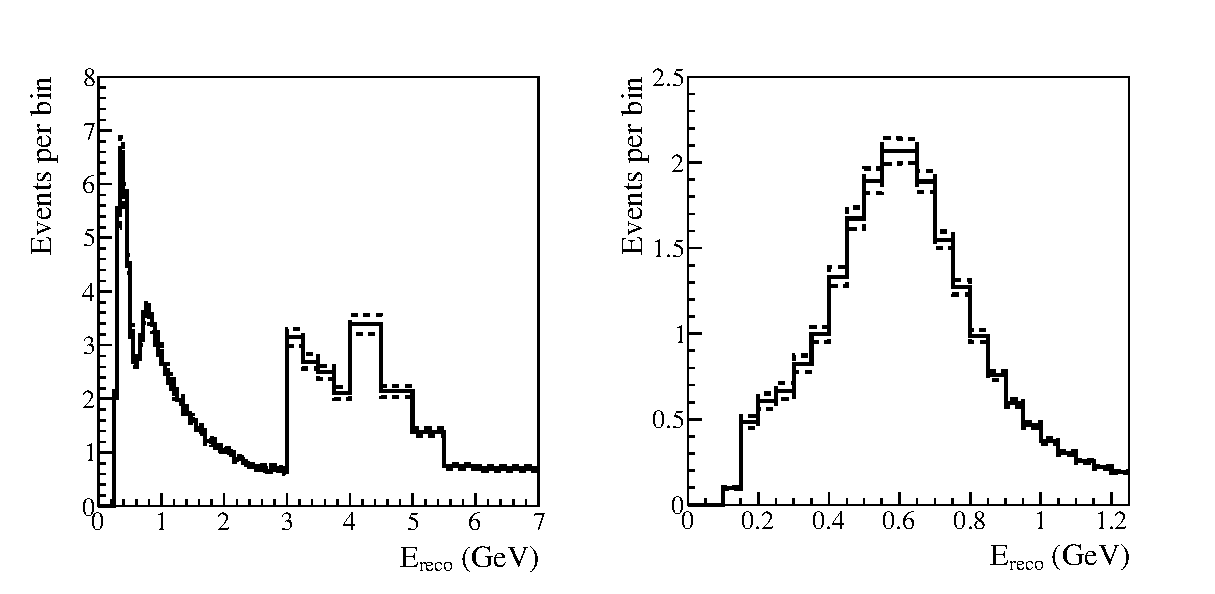
\includegraphics[width=30pc]{./images/systematics/Error_envelope_BANFF.eps}
\caption {
  Error envelope of the single $\mu$-like ring and single e-like event reconstructed energy spectra,
  for oscillations with typical values and the normal mass hierarchy assumed, for the BANFF systematic parameters.
  The numbers shown were calculated for an exposure of 6.5700$\times$10$^{20}$ POT.
  BANFF-tuned MC templates were used.
  The error envelope was calculated as the $\pm$1$\sigma$ spread of bin contents using an ensemble of 20k toy MC experiments generated with randomized BANFF systematic parameters, taking into account their correlations.
}
\label{fig:error_envelope_banff}
\end{figure*}


\begin{figure*}[htb]
\center
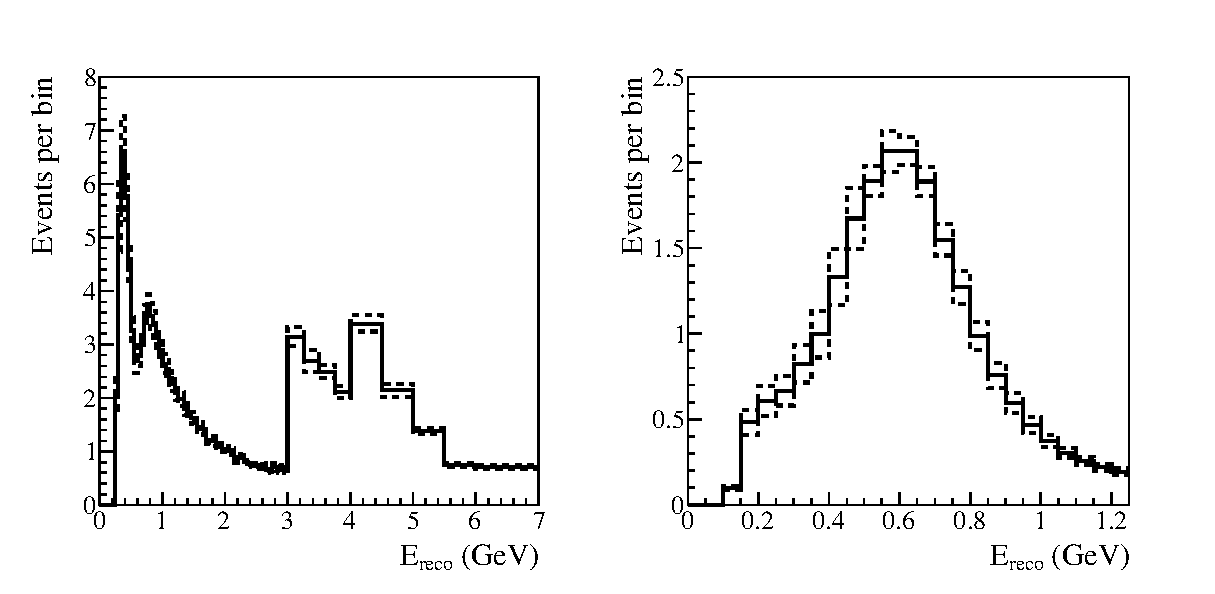
\includegraphics[width=30pc]{./images/systematics/Error_envelope_xsec.eps}
\caption {
  Error envelope of the single $\mu$-like ring and single e-like event reconstructed energy spectra,
  for oscillations with typical values and the normal mass hierarchy assumed, for the uncorrelated cross-section systematic parameters.
  The numbers shown were calculated for an exposure of 6.5700$\times$10$^{20}$ POT.
  BANFF-tuned MC templates were used.
  The error envelope was calculated as the $\pm$1$\sigma$ spread of bin contents using an ensemble of 20k toy MC experiments generated with randomized uncorrelated cross-section systematic parameters.
}
\label{fig:error_envelope_xsec}
\end{figure*}


\begin{figure*}[htb]
\center
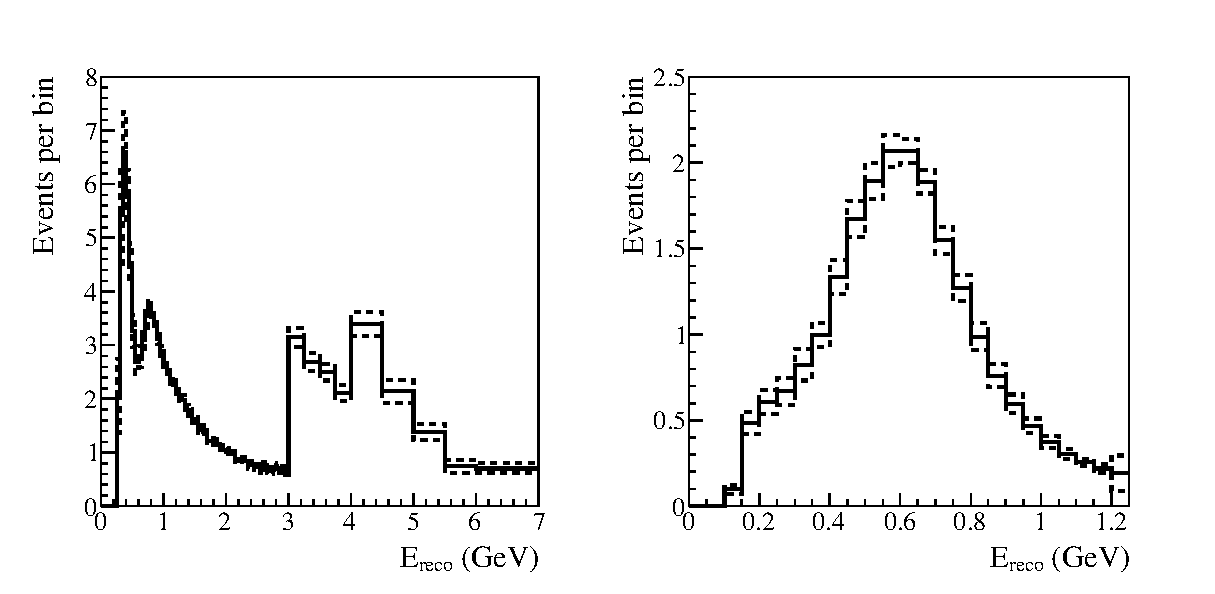
\includegraphics[width=30pc]{./images/systematics/Error_envelope_skfsi_final.eps}
\caption {
  Error envelope of the single $\mu$-like ring and single e-like event reconstructed energy spectra,
  for oscillations with typical values and the normal mass hierarchy assumed, for the SK+FSI systematic parameters.
  The numbers shown were calculated for an exposure of 6.5700$\times$10$^{20}$ POT.
  BANFF-tuned MC templates were used.
  The error envelope was calculated as the $\pm$1$\sigma$ spread of bin contents using an ensemble of 20k toy MC experiments generated with randomized SK+FSI systematic parameters, taking into account their correlations.
}
\label{fig:error_envelope_skfsi}
\end{figure*}

\begin{figure*}[htb]
\center
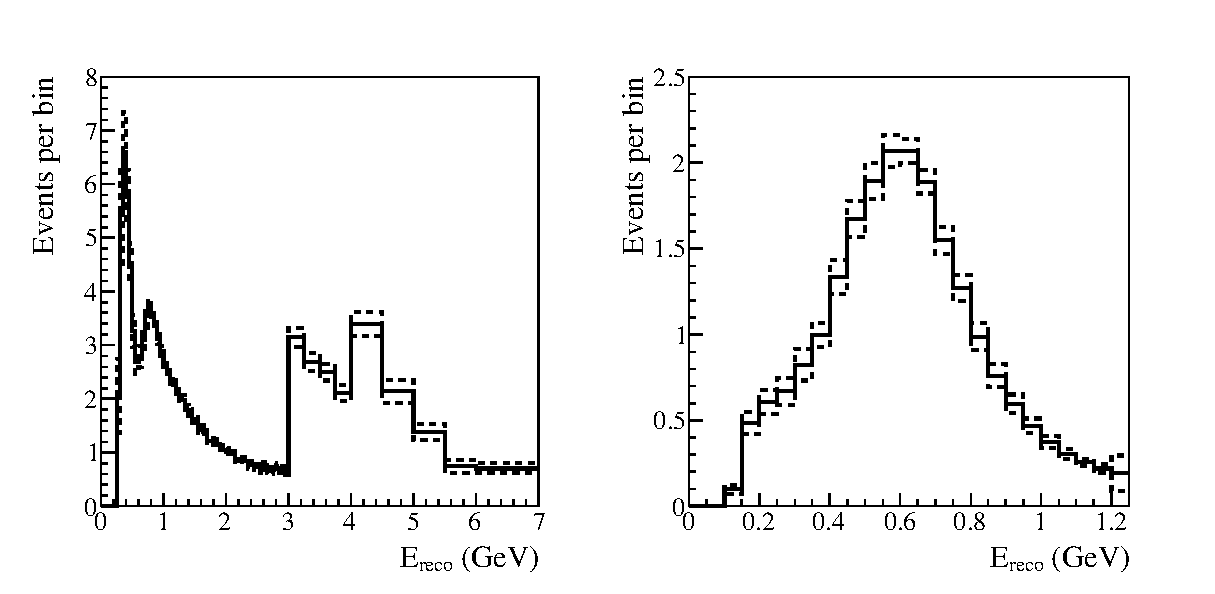
\includegraphics[width=30pc]{./images/systematics/Error_envelope_skfsi_final.eps}
\caption {
  Total error envelope of the single $\mu$-like ring and single e-like event reconstructed energy spectra,
  for oscillations with typical values and the normal mass hierarchy assumed.
  The numbers shown were calculated for an exposure of 6.5700$\times$10$^{20}$ POT.
  BANFF-tuned MC templates were used.
  The error envelope was calculated as the $\pm$1$\sigma$ spread of bin contents using an ensemble of 20k toy MC experiments generated with all systematic parameters randomized, taking into account their correlations.
}
\label{fig:error_envelope_total}
\end{figure*}


\begin{figure*}[htb]
\center
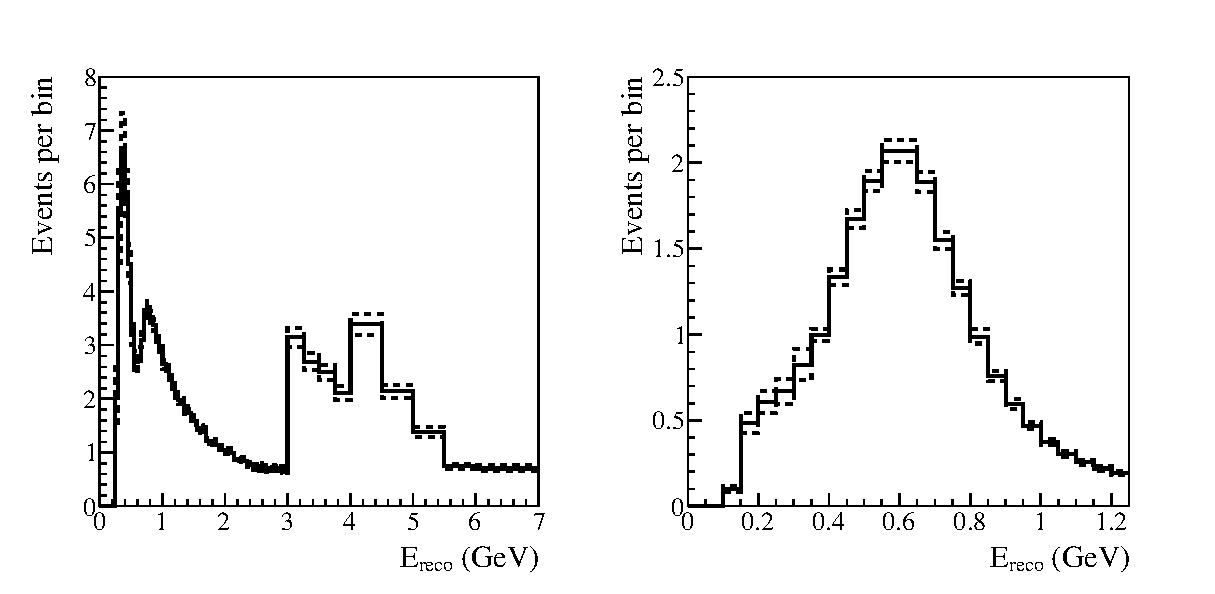
\includegraphics[width=30pc]{./images/systematics/Error_envelope_skfsi_final_noEscale.eps}
\caption {
As in Fig. \ref{fig:error_envelope_skfsi}, but not tweaking the reconstructed energy scale systematic. 
}
\label{fig:error_envelope_skfsi_noEscale}
\end{figure*}



\begin{figure*}[htb]
\center
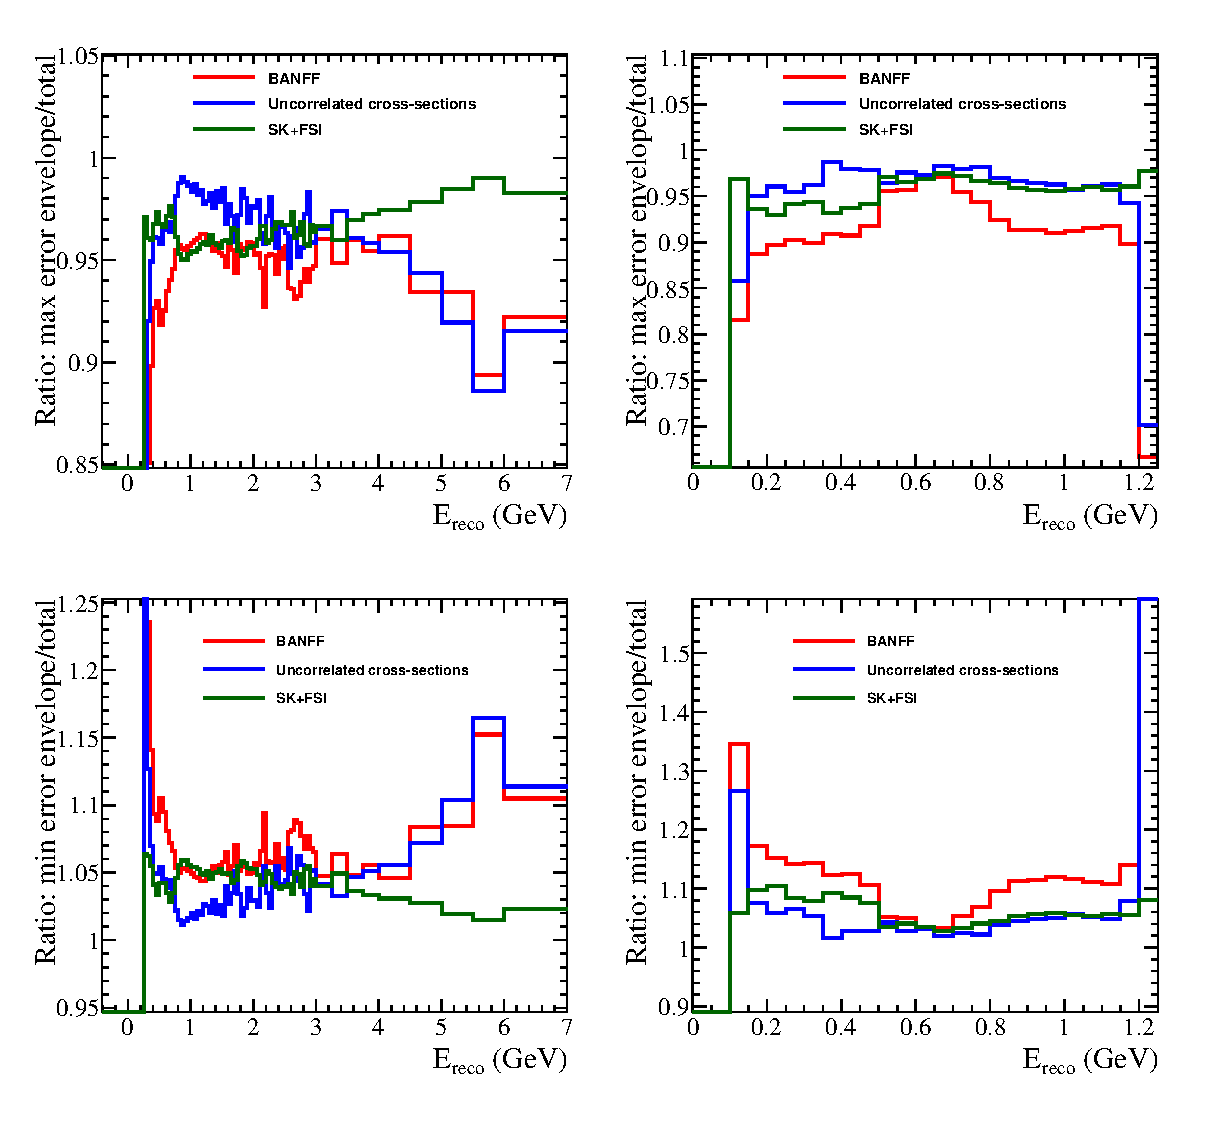
\includegraphics[width=30pc]{./images/systematics/Ratios_error_envelopes.eps}
\caption {
Ratios of the error envelopes in Figs. \ref{fig:error_envelope_banff}-\ref{fig:error_envelope_skfsi} to the total error envelope in Fig. \ref{fig:error_envelope_total} for the maximum (top plots) and minimum (bottom plots) spread.
}
\label{fig:error_envelope_ratios}
\end{figure*}

%..................






\clearpage

\section{Neutrino oscillation fitting}
\label{sec:neutrino_oscillation_fitting}


\subsection{Minimization method}

The {\em VaLOR} joint 3-flavour analysis uses a binned likelihood-ratio method.
Measurements of the oscillation parameters
$|\Delta m^{2}|$, $\sin^{2}\theta_{23}$, $\sin^{2}\theta_{13}$ and $\delta_{CP}$\footnote{
   A study has been made in which $\sin^{2}\theta_{12}$ and $\delta m^{2}$ were allowed to float in the fit and 
   the results are shown in Appendix \ref{app:solar}. 
   The effect was negligible and, in the analysis reported here, they were simply fixed to
   $\sin^{2}\theta_{12}$ = 0.311 and $\delta m^{2}$ = 7.5$\times$10$^{-5}$ eV$^{2}$/c$^{4}$.
}
are obtained by comparing the observed and predicted reconstructed single $\mu$-like ring and single e-like ring energy spectra in SuperK. 
Let $N_{\mu}$ and $N_{e}$ be the numbers of reconstructed energy bins considered for the single $\mu$-like ring and
single e-like ring samples respectively, 
and
${\bf a}$ be a $1 \times N_{s}$ - dimensional array of systematic (nuisance) 
parameters that affect the SuperK reconstructed energy spectrum prediction of either sample 
e.g. parameters that control the beam, neutrino interaction simulations and 
the detector response.
Best-fit values are obtained by minimizing: 

\begin{equation}
\begin {split}
\displaystyle
%\chi^{2}   &=                                                                                                                                                                                       
 -2 \, \textrm{ln} \lambda (|\Delta m^{2}|, sin^{2}\theta_{23}, \sin^{2}\theta_{13}, \delta_{CP}; {\bf a}) &=
  2 \cdot \sum_{r=0}^{N_{\mu}-1}
   \left[
    (N^{exp}_{SK;\mu,r}-N^{obs}_{SK;\mu,r}) + 
     N^{obs}_{SK;\mu,r} \cdot ln\left(\frac{N^{obs}_{SK;\mu,r}}{N^{exp}_{SK;\mu,r}}\right)  
   \right]  \\
    \displaystyle
    &+ 2 \cdot \sum_{r=0}^{N_{e}-1}
    \left[
    (N^{exp}_{SK;e,r}-N^{obs}_{SK;e,r}) + 
     N^{obs}_{SK;e,r} \cdot ln\left(\frac{N^{obs}_{SK;e,r}}{N^{exp}_{SK;e,r}}\right)  
   \right]  \\
  &+  ({\bf a}-{\bf a_{0}})^{T} \cdot {\bf C}^{-1} \cdot ({\bf a}-{\bf a_{0}})
\label{eq:chisquare}
\end{split}
\end{equation}
where
$N^{obs}_{SK;\mu,r}$ ($N^{obs}_{SK;e,r}$) is the observed number of single $\mu$-like ring (single e-like ring) events in the $r^{th}$ bin, 
and $N^{exp}_{SK;\mu,r}$ ($N^{exp}_{SK;e,r}$)
is the corresponding expected number of events; this expected number is a function of 
$|\Delta m^{2}|$, $\sin^{2}\theta_{23}$, $\sin^{2}\theta_{13}$ and $\delta_{CP}$
and the nuisance parameter vector ${\bf a}$.
Also ${\bf a_{0}}$ is a $1 \times N_{s}$ - dimensional array containing the nominal values of
the systematic parameters, ${\bf a}^{T}$ is the transpose of ${\bf a}$,
and ${\bf C}$ is the systematic parameter covariance matrix of dimension $N_{s} \times N_{s}$.
For the stand-alone $\nu_{\mu}$-disappearance ($\nu_{e}$-appearance) fit, 
only the single $\mu$-like ring (single e-like ring) sample is used and the 
corresponding term in Eq.\ \ref{eq:chisquare} is dropped.

The likelihood-ratio method used in this analysis is equivalent to the extended maximum likelihood
method used in the alternative T2K oscillation analysis 
(see \cite{OurRun1DisappAnalysis,StatAnalysisCowan} for more details).
The advantage of the likelihood-ratio method, compared with the extended maximum-likelihood method, is that
in the large-sample limit, the quantity $-2 \, \textrm{ln} \lambda (|\Delta m^{2}|, \sin^{2}\theta_{23}, \sin^{2}\theta_{13}, \delta_{CP}; {\bf a})$
in Eq.\ref{eq:chisquare} has a $\chi^{2}$ distribution and it can therefore be used as a goodness-of-fit test.
In this note
$-2 \, \textrm{ln} \lambda (|\Delta m^{2}|, \sin^{2}\theta_{23}, \sin^{2}\theta_{13}, \delta_{CP}; {\bf a})$ and
$\chi^{2}(|\Delta m^{2}|, \sin^{2}\theta_{23}, \sin^{2}\theta_{13}, \delta_{CP}; {\bf a})$ are used interchangeably. 

In the joint 3-flavour oscillation analysis fits, all 83 systematic parameters are allowed to float, whereas 
in the stand-alone analyses (which use a single SuperK sample) only the relevant systematics are used (see Tab.\ \ref{tab:apply_syst_to_samples}).

The search for the minimum value of 
$-2 \, \textrm{ln} \lambda(|\Delta m^{2}|, \sin^{2}\theta_{23}, \sin^{2}\theta_{13}, \delta_{CP}; {\bf a})$
is performed in the range 
1.0 $\times$10$^{-3}$ eV$^{2}$/c$^{4}$ $\leq$ $|\Delta m^{2}|$ $\leq$ 6.0 $\times$10$^{-3}$ eV$^{2}$/c$^{4}$,
0.0 $\leq$ $\sin^{2}\theta_{23}$ $\leq$ 1.0,
0.0 $\leq$ $\sin^{2}\theta_{13}$ $\leq$ 1.0 and
$-\pi$ $\leq$ $\delta_{CP}$ $\leq$ $\pi$.
Systematic parameters included in the oscillation fit are constrained in the range [-2$\sigma_{s}$, +2$\sigma_{s}$]
where $\sigma_{s}$ is the one standard deviation error assigned to each systematic parameter\footnote{
 Such an error is defined for all but one of the systematic parameters considered in this analysis. 
 The exception is the systematic parameter $f_{SF}$ which parametrises the uncertainty on nuclear modelling, 
 switching between the Relativistic Fermi Gas (RFG) and Spectral Function (SF) models. The allowed range of the parameter $f_{SF}$ 
in the oscillation fit is [0,1].}. Validations studies were done with systematic parameters fitted in a wider range 
[-5$\sigma_{s}$, +5$\sigma_{s}$] with no difference in the results. However, the Run1+2+3 data fit will be updated with
a wider range such as [-5$\sigma_{s}$, +5$\sigma_{s}$] . 
Values of systematic parameters that give a negative predicted number of events in any reconstructed energy bin are not allowed. 
If this scenario arises, the number of events is changed to +1E-8 in that bin. This is done for the sum of all the interaction 
modes rather than for each mode separately.

The minimization is performed with Minuit \cite{Minuit}, using the Migrad method.
If Migrad does not converge, the starting values of the oscillation parameters are re-initialised:
the new initial values are randomly drawn from uniform distributions in the ranges 
$2.0 \cdot 10^{-3}$ $\leq$ $|\Delta m^{2}|$ $\leq$ $3.0 \cdot 10^{-3}$,
0.35 $\leq$ sin$^{2}\theta_{23}$ $\leq$ 0.65, 
0.015 $\leq$ sin$^{2}\theta_{13}$ $\leq$ 0.035
and the fit is retried. This is repeated 25 times.
If the fits still fail to converge, the Simplex algorithm is used.

%..................................
%

\subsection{Goodness-of-fit tests}
\label{sec:goodness_of_fit}
The problem of defining a general goodness-of-fit for sparsely populated distributions
was discussed in detail during the development of the Run 1+2+3 stand-alone $\nu_\mu$-disappearance 
and $\nu_{e}$-appearance analyses. See for example \cite{KarlenPvalue}.
It was pointed out that, for the Run 1+2+3 statistics, the shape information is not
as helpful in forming p-values as the rate information.
It was decided that  p-values will be calculated using the rate and the reconstructed energy distribution,
and that the distribution will use a very coarse binning
scheme to ensure that there are sufficient numbers of events in each bin.

A similar approach is used for the joint 3-flavour analysis presented here.
For the single $\mu$-like ring sample, 5 reconstructed energy bins are used:
0-0.4, 0.4-0.7, 0.7-1.0, 1.0-2.0 and 2.0-30.0 GeV.
For the single e-like ring sample, 3 reconstructed energy bins are used:
0-0.35, 0.35-0.80, 0.80-1.25 GeV.
In this note, p-values for the joint 3-flavour fit are computed following 
the 5+3 binning scheme described above. When p-values are quoted for the stand-alone
$\nu_{\mu}$-disappearance ($\nu_{e}$-appearance) analysis, the corresponding 
5 (3) bin scheme of the single $\mu$-like ring (single e-like ring) event sample is used.

The goodness-of-fit tests that will be shown are built using 1000 toy MC experiments
created at the best-fit point to be tested, with statistical and systematic fluctuations.
Then, each toy MC experiment is fitted in the coarse binning described above, 
including the four oscillation parameters and all systematics in the joint 3-flavour fit.
For the stand-alone disappearance the fit is performed for $sin^{2}\theta_{23}, \Delta m^{2}$ 
and the relevant systematics, being the other two oscillation parameters $sin^{2}\theta_{13}, \delta_{CP}$
fixed to the usual values.
For the stand-alone appearance the fit is performed for $sin^{2}\theta_{13}$
and the relevant systematics, being the other oscillation parameters
fixed to the usual values (with maximal mixing $sin^{2}\theta_{23} = 0.5$ and $\delta_{CP}=0$).


%..................................
%

\subsection{Toy-MC study of fitter performance}

The performance of the fitter has been evaluated using ensembles of 1k toy MC experiments
generated at different oscillation points with an exposure of $3.010\times10^{20}$ POT.
Two kinds of studies were performed with toy MC experiments. First, the simulated experiments
included only statistical fluctuations and were fitted with the '4 + 0' fit, i.e. fitting only for oscillation parameters.
A second ensemble of toy MC experiments including not only statistical fluctuations but also fluctuations of all
systematic parameters was created. Those toy MC experiments were fitted with the '4 + 83' fit, i.e. fitting for 
oscillation parameters and for all systematic parameters. No issue was identified regarding the fitter
performance, the results from these studies were as expected. 
In addition, the distributions of  residuals for the oscillation parameters
from both studies, doing '4 + 0' or '4 + 83' fits are consistent, indicating that no unexpected features 
appear when including fluctuations of the systematic parameters and when fitting for them. 
 
%..................................
%

\subsection{Construction of confidence regions}

In the analysis reported here, confidence regions are constructed using the constant $\Delta\chi^2$ method.
68\% and 90\% CL limits will be reported for each of $|\Delta m^{2}|$, $sin^{2}\theta_{23}$, $sin^{2}\theta_{13}$ and $\delta_{CP}$
oscillation parameters. In addition, 2-dimensional confidence regions for 68\% and 90\% CL will be shown for the following combinations of parameters: 
($sin^{2}\theta_{23}$, $|\Delta m^{2}|$),
($sin^{2}\theta_{13}$, $|\Delta m^{2}|$),
($sin^{2}\theta_{13}$, $\delta_{CP}$) and
($sin^{2}\theta_{23}$, $sin^{2}\theta_{13}$).

The first step to construct confidence contours in an oscillation parameter space 
is to build the $\Delta\chi^2$ surface in that space.
The oscillation parameter space is divided into a regular grid.
The following grid spacing is used in all confidence region construction methods:
$\delta{|\Delta{m^{2}}|}=0.05\times10^{-3} eV^{2}/c^{4}$,
$\delta{\sin^{2}\theta_{23}}=0.01$,
$\delta{\sin^{2}\theta_{13}}=0.005$ and
$\delta(\delta_{CP})= 2\pi/50$.
For the joint 3-flavour analysis confidence regions,
the $\chi^2$ is minimized at each grid point with respect to all 83 nuisance parameters considered in this analysis
and all oscillation parameters not shown on the plot (and not considered to be fixed).
For the stand-alone analyses, only the relevant systematics were used. 

The confidence regions for the joint analysis are constructed by finding the global best-fit point
(fitting all oscillation parameters and all systematic parameters at the same time)
and calculating the lines of {\em constant} $\Delta{\chi^{2}}$ from this point\footnote{
For 1 fit parameter, the critical values of $\Delta{\chi^{2}}$ used are 
1.00 (68\% CL), 2.71 (90\% CL), 3.84 (95\% CL), 6.63 (99\% CL).
For 2 parameters fitted simultaneously, the critical values of $\Delta{\chi^{2}}$ used are 
2.30 (68\% CL), 4.61 (90\% CL), 5.99 (95\% CL), 9.21 (99\% CL).
}. In the case of the stand-alone appearance analysis, a special procedure is followed 
to construct the confidence regions in ($sin^{2}\theta_{13}$, $\delta_{CP}$) space
 imitating the actual stand-alone analyses in T2K. In this method, called \textit{raster scan}, a best-fit
 value of  $sin^{2}\theta_{13}$ is found for each fixed value of $\delta_{CP}$, resulting in a line
 of best-fit points instead of a single best-fit point. Then, confidence intervals in $sin^{2}\theta_{13}$
 at a fixed $\delta_{CP}$ are found with respect to each best-fit $sin^{2}\theta_{13}$ using the 1D
 $\Delta{\chi^{2}}$ critical values \cite{FeldmanCousins}.

A full Feldman-Cousins construction in the 4-dimensional
($|\Delta m^{2}|$, $sin^{2}\theta_{23}$, $sin^{2}\theta_{13}$ and $\delta_{CP}$) space,
including all 83 systematics, is computationally prohibitive.
This analysis produces limits on each of the 4 oscillation parameters and, also,
confidence regions in 4 2-dimensional surfaces within the 4-dimensional oscillational parameter space.
There is no established procedure on how to sample the 4-dimensional oscillation space
and generate a toy-MC ensemble for the calculation of the critical $\Delta{\chi^{2}}$ values
needed for producing the limits or the 2-dimensional contours. We were confronted with
this issue both for the Run 1+2 disappearance analysis PRD paper
and the Run 1+2+3 disappearance analysis PRL paper, but no satisfactory solution was found.
We are aware that the same issue has baffled other collaborations too.
In the presence of this ambiguity over how to produce profile Feldman-Cousins contours, we propose
that this analysis produces contours only using the constant $\Delta{\chi^{2}}$ method.
Coverage studies are presented in Sec. \ref{app:coverage}.
If a non-ambiguous procedure is found,
based on our experience running the  Feldman-Cousins confidence region construction for the $\nu_{\mu}$-disappearance analysis,
we estimate that about $\sim$50,000 CPU$\cdot$days would be needed for the joint analysis.
The VaLOR group could prepare these contours in the time-scale of two months.


	
\clearpage

\section {Results of the joint oscillation analysis with the Run 1+2+3 ($3.010 \times 10^{20}$ POT) dataset}
\label{sec:results}

\subsection {Best-fit oscillation parameters and systematic parameter pulls}
\label{sec:results_bestfit_params}

A joint 3-flavour oscillation fit, 
using the method described in Sec.\ \ref{sec:neutrino_oscillation_fitting}
was performed simultaneously on the 
single e-like ring and single $\mu$-like ring event reconstructed energy spectra
of the 3.010$\times$10$^{20}$ POT Run 1+2+3 dataset.
This fit allowed all 83 nuisance parameters considered in this work to float.
This analysis found
$|\Delta m^{2}|$ = 2.494 $\times$10$^{-3}$ $eV^{2}/c^{4}$,
$\sin^{2}\theta_{23}$ = 0.516,
$\sin^{2}\theta_{13}$ = 0.029 and
$\delta_{CP}$ = 2.086
to be the joint 3-flavour oscillation best-fit values for the Run 1+2+3 dataset for Normal Hierarchy
and 
$|\Delta m^{2}|$ =  2.468 $\times$10$^{-3}$ $eV^{2}/c^{4}$,
$\sin^{2}\theta_{23}$ = 0.516,
$\sin^{2}\theta_{13}$ = 0.034 and
$\delta_{CP}$ = 0.921
for Inverted Hierarchy.

Stand-alone 3-flavour $\nu_{\mu}$ disappearance and $\nu_{e}$ appearance analyses
were also performed on the Run 1+2+3 dataset.
In the stand-alone $\nu_{\mu}$ disappearance analysis,
$|\Delta m^{2}|$ and $\sin^{2}\theta_{23}$ were determined by fitting the 
single $\mu$-like ring event reconstructed energy spectrum
keeping $\sin^{2}\theta_{13}$ and $\delta_{CP}$ fixed, as was done in our published result,
and allowing all 57 nuisance parameters relevant to this analysis to float.
Similarly, in the stand-alone $\nu_{e}$ appearance analysis, 
$\sin^{2}\theta_{13}$ and $\delta_{CP}$ were determined by fitting the 
single e-like ring event reconstructed energy spectrum,
keeping $|\Delta m^{2}|$ and $\sin^{2}\theta_{23}$ fixed, as was done in our published result,
and allowing all 69 nuisance parameters relevant to this analysis to float.
The results of these fits are summarized in Tab.\ \ref{tab:data_fits:best_fit_values}. 
In this table are 
the relevant best-fit oscillation parameters, 
the observed and expected number of single e-like ring and single $\mu$-like ring events,
and goodness-of-fit figures.
Notice that the best-fit value for $\sin^{2}\theta_{23}$ is the same in both hierarchies 
although the best-fit value for the other parameters is different. The reason for this
result will be investigated in Sec. \ref{app:symmetry}.

The pull for each systematic parameter f included in the fit, is calculated as
\begin{equation}
\frac{f_{bf} - f_{nom}}{\sigma_{bf}},
\end{equation}
where 
$f_{bf}$ is the best-fit value of the systematic parameter,
$f_{nom}$ is the nominal value of the parameter (corresponding to no systematic variation), and
$\sigma_{bf}$ is the Migrad error output from Minuit.
The pulls of all systematic parameters allowed to float in the joint 3-flavour oscillation fit to the Run 1+2+3 dataset are shown in 
Figs.\ \ref{fig:run123_pulls_NH} for the fit assuming Normal Hierarchy, and in Fig.\ \ref{fig:run123_pulls_IH} for the fit assuming Inverted Hierarchy.
From these figures, it is apparent that most systematic parameters barely move from their nominal values.
We note that, although all relevant systematic parameters are allowed to float in these fits,
few of them move by more than $\pm$0.1$\sigma$. 
When a systematic parameter that is free to move stays close to its nominal value, this means that 
the reduction in $\chi^{2}$ from moving that parameter is less than the corresponding increase 
in the penalty term in equation \ref{eq:chisquare}. 
Only certain systematics are able to change the predicted reconstructed energy spectrum to a 
sufficient extent to offset the penalty term.

\subsection {Goodness-of-fit tests}
\label{sec:results_gof}

Goodness-of-fit tests were performed as described in Sec.\ \ref{sec:goodness_of_fit},
and the p-values for the joint 3-flavour oscillation fit and
the stand-alone $\nu_{\mu}$ disappearance and $\nu_{e}$ appearance fits to the Run 1+2+3 dataset
are shown in Tab.\ \ref{tab:data_fits:best_fit_values}. 
The $\chi^2$ distributions from which the p-values were calculated are shown for the 
Run 1+2+3 joint 3-flavour oscillation fit in Fig.\ \ref{fig:run123_gofchisq} (\ref{fig:run123_gofchisq_ih}),
while for the stand-alone $\nu_{\mu}$ disappearance fit it is shown in Fig.\ \ref{fig:run123_gofchisq_disapp} (\ref{fig:run123_gofchisq_disapp_ih}) 
and for the stand-alone $\nu_{e}$ appearance it is shown in Fig.\ \ref{fig:run123_gofchisq_app} ( \ref{fig:run123_gofchisq_app_ih})
for Normal (Inverted) Hierarchy. All fits have a high degree of plausibility.


%...........................................................
%
% Table summarizing best-fit results
%
\begin{table}[htb]
\scriptsize
\centering
\begin{tabular}{| l | l | l | c  c  c  c | c  c  c  c | c  c |}
\hline
Analysis & Run & Hierarchy/ &
$|\Delta m^{2}|$ & sin$^2\theta_{23}$ & sin$^2\theta_{13}$ & $\delta_{CP}$ & 
N$_{obs}^{1R\mu}$ & N$_{exp}^{1R\mu}$ & 
N$_{obs}^{1Re}$ & N$_{exp}^{1Re}$ & 
$\chi^2/ndf$ & p-value \\
 &  & Octant & $10^{-3} eV^{2}/c^{4}$ & & & & & & & & & \\
\hline
2012 joint              & 1+2+3 & NH/1st & 2.494 & 0.516 & 0.029 & 2.086 &    58 & 57.697 & 11 & 10.452 & 72.26/94 & 0.86 \\
2012 $\nu_{\mu}$ disap. & 1+2+3 & NH/1st & 2.479 & 0.514 & --    & --    &    58 & 57.901 & 11 & --    & 56.05/71 & 0.90 \\
2012 $\nu_{e}$ app.     & 1+2+3 & NH/1st & --    & --    & 0.023 & 0(fixed) &    58 & --    & 11 & 10.477 & 16.47/24 & 0.67 \\
\hline
2012 joint              & 1+2+3 & NH/2nd & 2.493 & 0.516 & 0.029 & 2.074 &      58 & 57.712 & 11 & 10.452 & 72.26/94 &  \\
2012 $\nu_{\mu}$ disap. & 1+2+3 & NH/2nd & 2.479 & 0.514 & --    & --    &     58 & 57.903 & 11 & --    & 56.05/71 &  \\
2012 $\nu_{e}$ app.     & 1+2+3 & NH/2nd & --    & --    & 0.023 & 0(fixed) &     58 & --    & 11 & 10.477 & 16.47/24 &  \\
\hline
2012 joint              & 1+2+3 & IH/1st & 2.468 & 0.516 & 0.034 & 0.921 &      58 & 57.715 & 11 & 10.454 & 72.26/94 & 0.85 \\
2012 $\nu_{\mu}$ disap. & 1+2+3 & IH/1st & 2.474 & 0.512 & --    & --    &      58 & 57.891 & 11 & --    & 56.05/71 & 0.90 \\
2012 $\nu_{e}$ app.     & 1+2+3 & IH/1st & --    & --    & 0.029 & 0(fixed) &     58 & --    & 11 & 10.435 & 16.42/24 & 0.58 \\
\hline
2012 joint              & 1+2+3 & IH/2nd & 2.468 & 0.516 & 0.034 & 0.922 &      58 & 57.723 & 11 & 10.454 & 72.26/94 &  \\
2012 $\nu_{\mu}$ disap. & 1+2+3 & IH/2nd & 2.474 & 0.512 & --    & --    &    58 & 57.891 & 11 & --    & 56.05/71 &  \\
2012 $\nu_{e}$ app.     & 1+2+3 & IH/2nd & --    & --    & 0.029 & 0(fixed) &     58 & --    & 11 & 10.435 & 16.42/24 &  \\
\hline
\end{tabular}
\caption{
  Summary of best-fit parameters for the joint 3-flavour oscillation fit,
  and the stand-alone 3-flavour $\nu_{\mu}$ disappearance and $\nu_{e}$ appearance fits
  to the Run 1+2+3 dataset.
  The quoted best-fit $\chi^2$ values were computed from the test-statistic minimized in the fit (likelihood ratio)
  with the reconstructed energy binning used in each fit.
  The table also shows the p-values obtained from the goodness-of-fit test of Sec.\ \ref{sec:goodness_of_fit}.
}
\label{tab:data_fits:best_fit_values}
\end{table}

%
% Spectra
%

\subsection {Best-fit single e-like ring and single $\mu$-like ring event reconstructed energy spectra}
\label{sec:results_bestfit_spectra}

The reconstructed neutrino energy distribution of single $\mu$-like ring (single e-like ring) events 
in the Run 1+2+3 dataset is shown in Fig.\ \ref{fig:run123_1Rmu_bestfit_spectrum_nh} (Fig.\ \ref{fig:run123_1Re_bestfit_spectrum_nh})
along with best-fit prediction of the joint 3-flavour oscillation analysis, assuming Normal Hierarchy.
In Fig.\ \ref{fig:run123_1Rmu_bestfit_spectrum_nh}
we superimpose the best-fit prediction from the stand-alone 3-flavour $\nu_{\mu}$ disappearance analysis,
while in In Fig.\ \ref{fig:run123_1Re_bestfit_spectrum_nh}
we superimpose the best-fit prediction from the stand-alone 3-flavour $\nu_{e}$ appearance analysis.
The distributions are shown with the reconstructed neutrino energy binning
that was used in the fitting procedure (see footnote 2 in Sec.\ \ref{sec:prediction}).
The single $\mu$-like ring (single e-like ring) 
best-fit prediction of the joint 3-flavour oscillation analysis, assuming Inverted Hierarchy,
are shown in Fig.\ \ref{fig:run123_1Rmu_bestfit_spectrum_ih} (Fig.\ \ref{fig:run123_1Re_bestfit_spectrum_ih}).

Since the reconstructed energy binning used in the fit is relatively fine, 
it can be beneficial to see the above distributions using a coarser binning scheme\footnote{
  For the single $\mu$-like ring event sample
  16 reconstructed energy bins are used arranged as follows:
  1 0.3-GeV bin in 0 - 0.3 GeV,
  8 0.1-GeV bins in 0.3 - 1.1 GeV,
  1 0.15-GeV bin in 1.1 GeV - 1.25 GeV,
  1 0.25-GeV bin in 1.25 - 1.5 GeV GeV,
  1 0.5-GeV bin in 1.5 - 2 GeV,
  2 1-GeV bin in 2-4 GeV,
  1 2-GeV bin in 4-6 GeV and 1 bin above 6 GeV.
  For the single e-like ring event sample 4 0.3 GeV bins in 0-1.2 GeV are used.
}. 
The re-binned reconstructed neutrino energy distribution of single $\mu$-like ring and single e-like ring events for both mass hierarchies
are shown in Figs.\ \ref{fig:run123_1Rmu_bestfit_spectrum_nh_coarse} - \ref{fig:run123_1Re_bestfit_spectrum_ih_coarse}.

Finally, the ratio of the best-fit reconstructed neutrino energy distribution of single $\mu$-like ring (single e-like ring)
events obtained from the joint 3-flavour oscillation analysis and the stand-alone  $\nu_{\mu}$ disappearance ( $\nu_{e}$ appearance) analysis
is shown in Fig.\ \ref{fig:run123_1Rmu_bestfit_spectrum_ratio_nh} (Fig.\ \ref{fig:run123_1Re_bestfit_spectrum_ratio_nh}) for Normal Hierarchy and
in Fig.\ \ref{fig:run123_1Rmu_bestfit_spectrum_ratio_ih} (Fig.\ \ref{fig:run123_1Re_bestfit_spectrum_ratio_ih}) for Inverted Hierarchy.

The best-fit single $\mu$-like ring reconstructed energy spectrum from the joint analysis is almost identical to that from the stand-alone $\nu_{\mu}$-disappearance analysis from 0.6 - 1.2 GeV, 
but is slightly lower from 0.3 - 0.6 GeV and $>$1.2 GeV, and this is true for both mass hierarchies. 
Meanwhile the ratio of the best-fit single e-like ring reconstructed energy spectrum from the joint analysis to that from the stand-alone $\nu_{e}$-appearance analysis 
shows different behaviour for the two hierarchies. For the normal hierarchy (NH), this ratio is $<$1 from 0.1 - 0.3 GeV, $>$1 from 0.3 - 0.55 GeV, and $<$1 above 0.55 GeV. 
However, for the inverted hierarchy (IH) the ratio is $<$1 from 0.1 - 0.6 GeV and $>$1 above 0.6 GeV. 

%
% Contours
%

\subsection {Confidence regions}
\label{sec:results_confidence_regions}

The marginalized $\Delta\chi^2$ distribution as function
of each of $|\Delta m^{2}|$, $sin^{2}\theta_{23}$, $sin^{2}\theta_{13}$ and $\delta_{CP}$
oscillation parameters for the joint 3-flavour oscillation fit to the Run 1+2+3 dataset 
is shown in Figs.\ \ref{fig:run123_dchisq_Dmsq_nh} - \ref{fig:run123_dchisq_deltacp_nh}.
From these plots,
the 90\% (68\%) CL allowed region for the four oscillation parameters can be summarized as
2.227$\times$10$^{-3}$ (2.332$\times$10$^{-3}$) $eV^{2}/c^{4}$
$< |\Delta m^{2}| < $
2.773$\times$10$^{-3}$ (2.659$\times$10$^{-3}$) $eV^{2}/c^{4}$,
0.401 (0.433) $< sin^{2}\theta_{23} <$ 0.628 (0.596),
0.006 (0.012) $< sin^{2}\theta_{13} <$ 0.058 (0.048) and
-$\pi$ (-$\pi$) $< \delta_{CP} <$ $\pi$ ($\pi$)
for Normal Hierarchy and
2.218 $\times$10$^{-3}$ (2.311$\times$10$^{-3}$) $eV^{2}/c^{4}$
$< |\Delta m^{2}| < $
2.729 $\times$10$^{-3}$ (2.627$\times$10$^{-3}$) $eV^{2}/c^{4}$,
 0.397 (0.433) $< sin^{2}\theta_{23} <$ 0.627 (0.596),
0.006 (0.013) $< sin^{2}\theta_{13} <$ 0.069 (0.054) and
-$\pi$ (-$\pi$) $< \delta_{CP} <$ $\pi$ ($\pi$)
for Inverted Hierarchy.

The correlations between the oscillation parameters were also studied.
In Figs.\ \ref{fig:run123_confreg_sinsqtheta23_Dmsq_nh} - \ref{fig:run123_confreg_sinsqtheta23_sinsqtheta13_nh}, 
we present, respectively, the 
the 68\% and 90\% CL regions in the following four 2-dimensional oscillation parameter spaces:
($sin^{2}\theta_{23}$, $|\Delta m^{2}|$),
($sin^{2}\theta_{13}$, $|\Delta m^{2}|$),
($sin^{2}\theta_{13}$, $\delta_{CP}$) and
($sin^{2}\theta_{23}$, $sin^{2}\theta_{13}$).
Results from the stand-alone Run 1+2+3 $\nu_{\mu}$ disappearance and $\nu_{e}$ appearance 
analyses are superimposed wherever possible.

Comparisons between the confidence regions obtain from the joint 3-flavour oscillation fits
under difference mass hierarchy assumptions are shown in Figs.\ \ref{fig:run123_dchisq_Dmsq_hcomp} - \ref{fig:run123_confreg_sinsqtheta23_sinsqtheta13_hcomp}.
%Comparisons between the confidence regions obtain from the joint 3-flavour oscillation fits, for the Normal Hierarchy,
%but using initial fit values in the different octants are shown in Figs.\ \ref{fig:run123_dchisq_Dmsq_octcomp} - \ref{fig:run123_confreg_sinsqtheta13_Dmsq_octcomp}.

To construct the plots shown in this subsection, the same procedure is followed 
as in Appendix \ref{app:fake_dataset_fits}.
In joint 3-flavour analysis plots,
the value of $\chi^2$ was minimized with respect to all 83 nuisance parameters
and the oscillation parameters not shown on the plot (except from the solar parameters,
$sin^{2}\theta_{12}$ and $\delta m^{2}$ which, as shown in Appendix \ref{app:solar}, 
have a negligible effect and they are fixed to constant values for all the joint and stand-alone analyses).
In the plots shown for the stand-alone $\nu_{\mu}$ disappearance analysis, unless explicitly stated,
$sin^{2}\theta_{13}$ and $\delta_{CP}$ are fixed to constant values,
as was done for our published results,
and $\chi^2$ was minimized with respect to all 48 nuisance parameters
relevant to that analysis.
Similarly, for the stand-alone $\nu_{e}$ appearance analysis, unless explicitly stated,
$sin^{2}\theta_{23}$ and $|\Delta m^{2}|$ are also fixed to constant values,
as was done for our published results,
and $\chi^2$ was minimized with respect to all 64 nuisance parameters
relevant to that analysis.

The $\Delta \chi^{2}$ distributions of $|\Delta m^{2}|$ and $\sin^{2}\theta_{23}$ are almost identical for the joint analysis and the stand-alone $\nu_{\mu}$-disappearance analysis. 
However the $\Delta \chi^{2}$ distribution of $\sin^{2}\theta_{13}$ is wider for the joint analysis than for the stand-alone $\nu_{e}$-appearance analysis. 
This is due to the partial degeneracy of this parameter with $\sin^{2}\theta_{23}$ when fitting the single e-like ring sample. Since $\sin^{2}\theta_{23}$ 
is fitted in the joint analysis, the $\Delta \chi^{2}$ distribution of $\sin^{2}\theta_{13}$ is wider than in the stand-alone analysis in which $\sin^{2}\theta_{23}$ is fixed. 
There is very good agreement between the confidence contours in the ($\sin^{2}\theta_{23}$, $|\Delta m^{2}|$) space from the joint analysis and those from the 
stand-alone $\nu_{\mu}$-disappearance analysis. Contours in the ($\sin^{2}\theta_{13}$, $\delta_{CP}$) space are wider for the joint analysis with respect to the contours
obtained for the stand-alone appearance analysis. The main reason is the different method used (global minimum vs raster scan). In Figs. \ref{fig:run123_confreg_sinsqtheta13_deltacp_raster_nh}
and \ref{fig:run123_confreg_sinsqtheta13_deltacp_raster_ih} the same method (raster scan) was used for both the joint and the stand-alone appearance analysis to fit
Run1+2+3 dataset in Normal and Inverted Hierarchy respectively. Contours from the joint analysis agree very well with those from the 
stand-alone $\nu_{e}$-appearance analysis when using the raster scan method in both analyses. 

The $\Delta \chi^{2}$ distributions for $|\Delta m^{2}|$ and $\sin^{2}\theta_{23}$  are very similar between the NH and IH. However the distribution for $\sin^{2}\theta_{13}$ 
and $\delta_{CP}$ is shifted to higher values for the IH compared with the NH, while the distribution for $\delta_{CP}$ is shifted to lower values. 
The confidence contours in the ($\sin^{2}\theta_{23}$, $|\Delta m^{2}|$) space agree very well between the NH and IH, but the upper 
limit in the ($\sin^{2}\theta_{13}$, $\delta_{CP}$) space is higher for the IH than for the NH.

%All the $\Delta \chi^{2}$ distributions and confidence regions agree very well between the initial value of $\sin^{2}\theta_{23}$ being in the first octant and in the second octant.


%...........................................................
%
% pulls
%

\begin{figure*}[htb]
\center
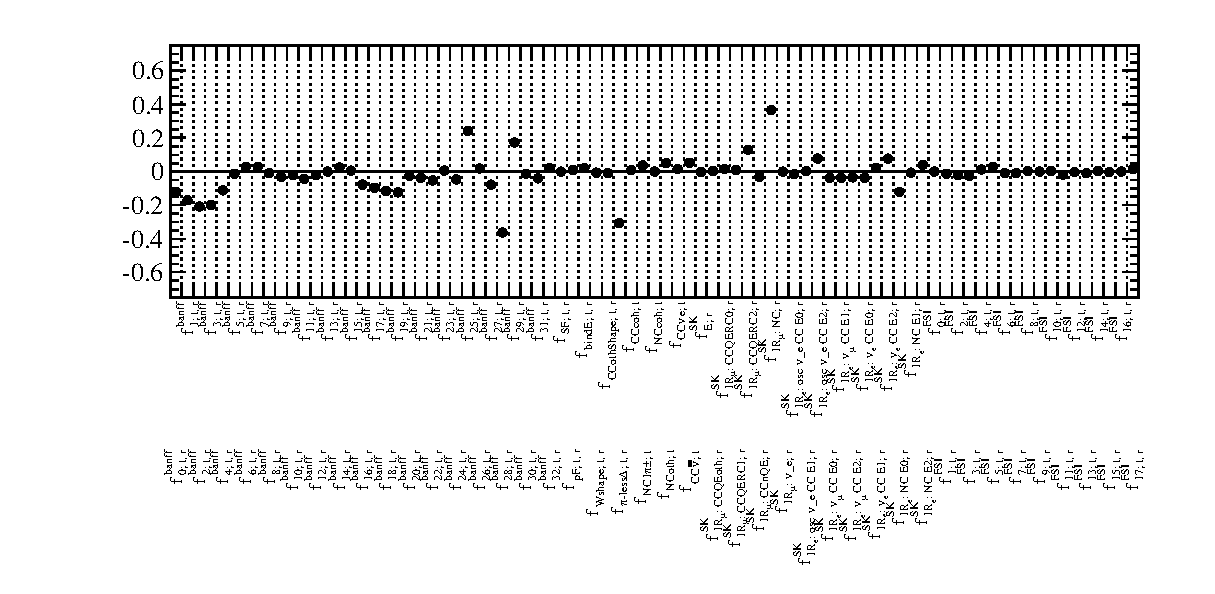
\includegraphics[width=55pc,angle=270]{./images/results/pulls_data_nh_1st.eps}
\caption {
  Systematic parameter pulls for the 83 systematics allowed to float 
  in the Run 1+2+3 joint 3-flavour oscillation fit with Normal Hierarchy.
}
\label{fig:run123_pulls_NH}
\end{figure*}

\begin{figure*}[htb]
\center
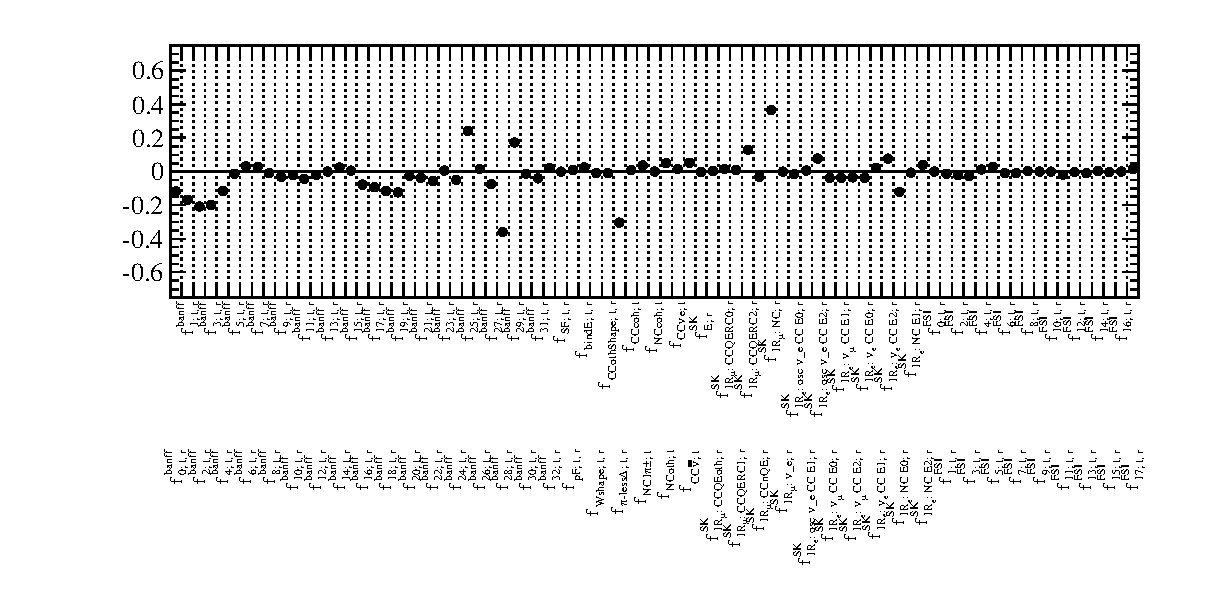
\includegraphics[width=55pc,angle=270]{./images/results/pulls_data_ih_1st.eps}
\caption {
  Systematic parameter pulls for the 83 systematics allowed to float 
  in the Run 1+2+3 joint 3-flavour oscillation fit with Inverted Hierarchy.
}
\label{fig:run123_pulls_IH}
\end{figure*}




%...........................................................
%
% chisq distributions used for calculating the fit p-values
%

\begin{figure*}[htb]

\begin{minipage}[t]{0.90\linewidth}
\center
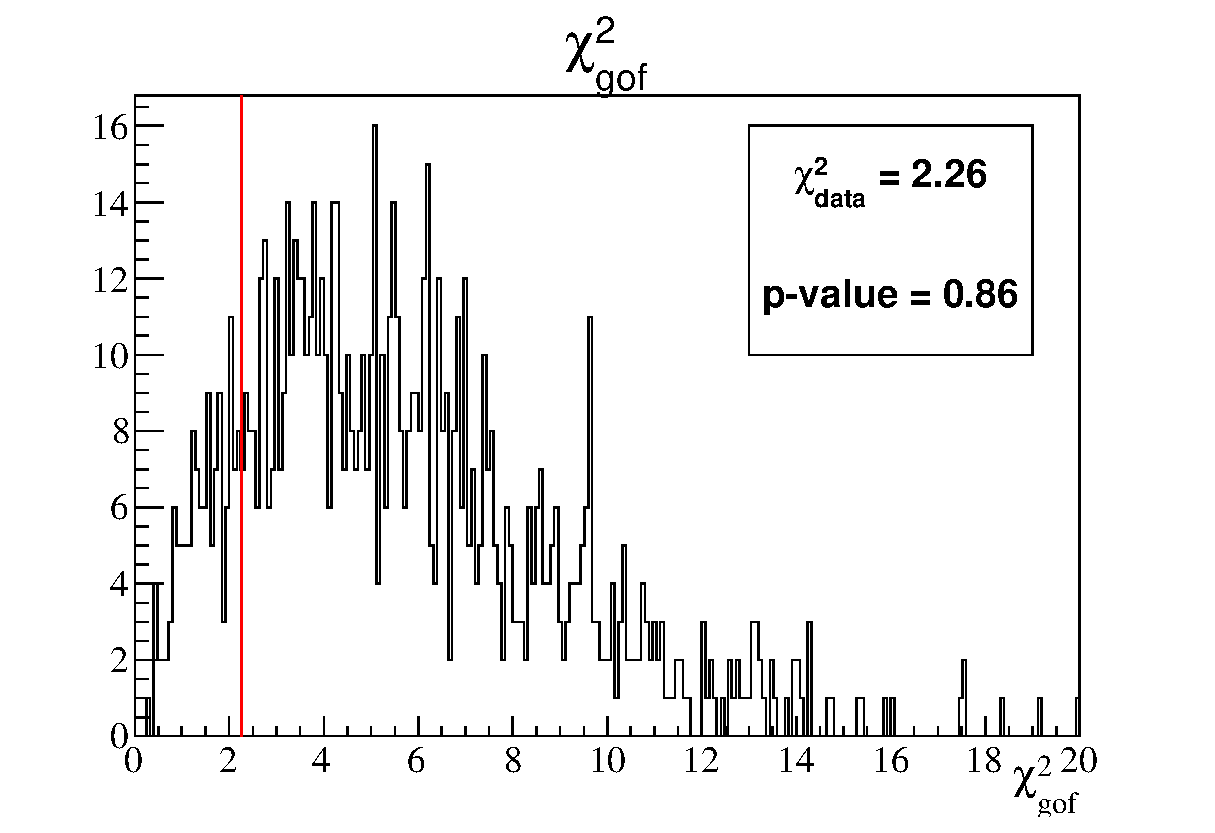
\includegraphics[width=30pc]{./images/results/data_nh_1st_gof_new.eps}
\caption {
  Distribution of $\chi^2_{gof}$, the goodness-of-fit (gof) $\chi^2$, 
  from 1k toy MC experiments generated at the Run 1+2+3 joint 3-flavour analysis best-fit oscillation point
  with Normal Hierarchy.
  The $\chi^2_{gof}$ value for the Run 1+2+3 data ($\chi^2_{data}$) is highlighted.
  All $\chi^2_{gof}$ values were computed 
  using the 5 (single $\mu$-like ring) + 3 (single e-like ring) 
  reconstructed energy binning scheme described in Sec.\ \ref{sec:goodness_of_fit},
}
\label{fig:run123_gofchisq}
\end{minipage}

\vfill
\vspace*{0.7cm}

\begin{minipage}[t]{0.46\linewidth}
\center
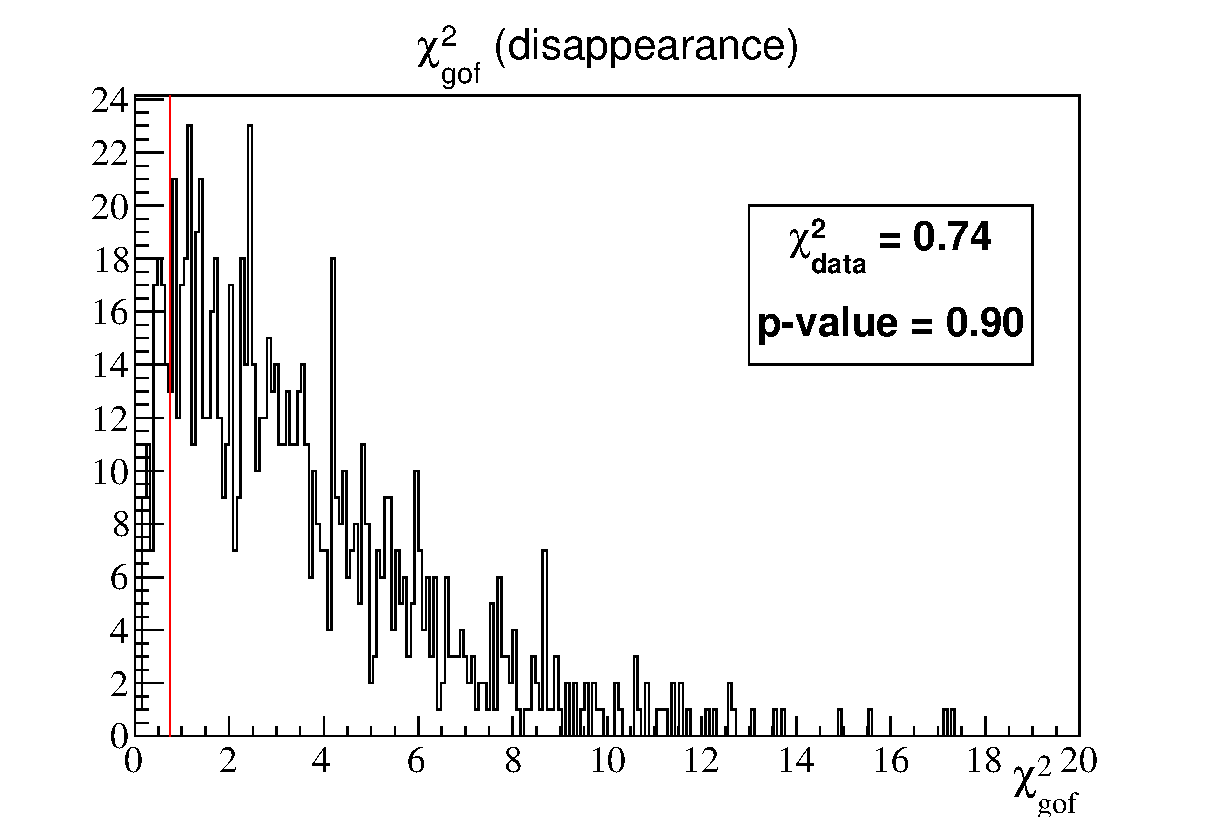
\includegraphics[width=18pc]{./images/results/data_nh_1st_gof_disap_new.eps}
\caption {
  Distribution of $\chi^2_{gof}$
  from 1k toy MC experiments generated at the Run 1+2+3 stand-alone 3-flavour $\nu_{\mu}$ disappearance analysis 
  best-fit oscillation point with Normal Hierarchy.
  The $\chi^2_{gof}$ value for the Run 1+2+3 data ($\chi^2_{data}$) is highlighted.
  All $\chi^2_{gof}$ values were computed 
  using the 5 (single $\mu$-like ring) 
  reconstructed energy binning scheme described in Sec.\ \ref{sec:goodness_of_fit},
}
\label{fig:run123_gofchisq_disapp}
\end{minipage}
\hspace{0.03\linewidth}
\begin{minipage}[t]{0.46\linewidth}
\center
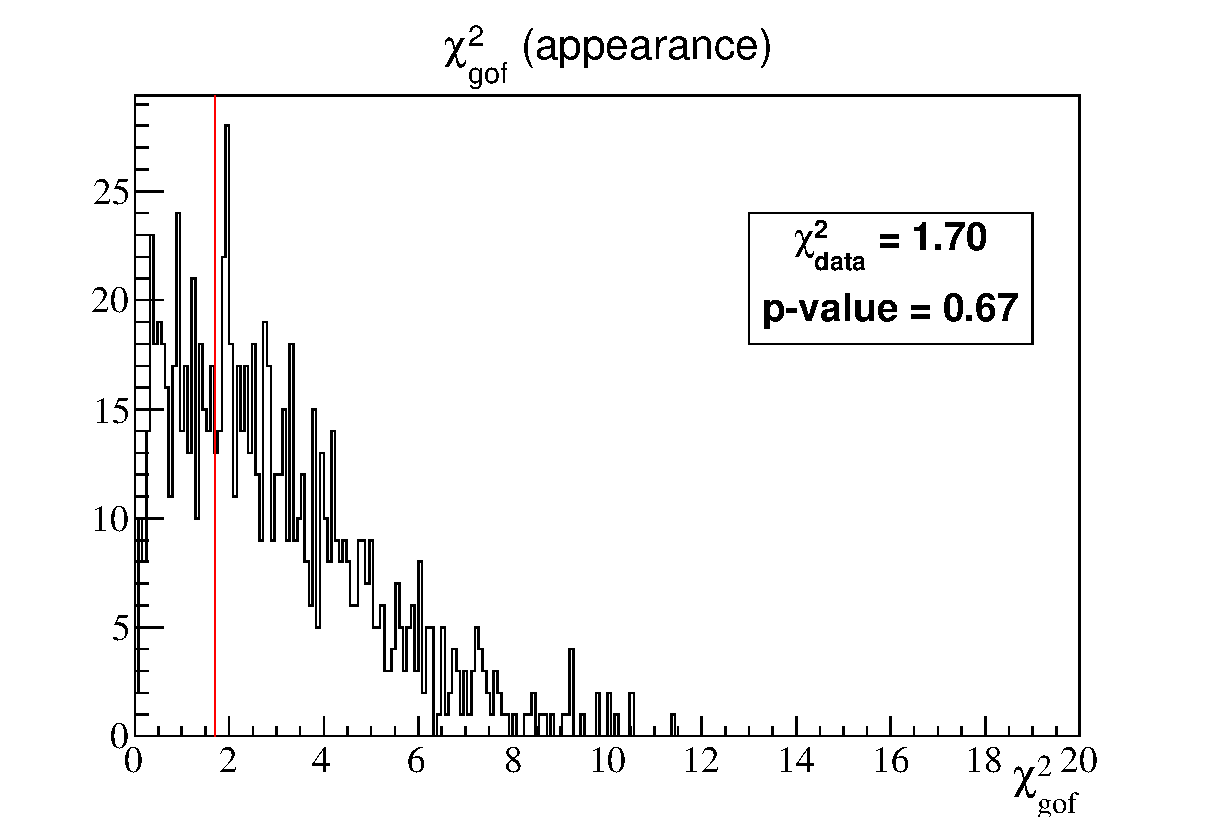
\includegraphics[width=18pc]{./images/results/data_nh_1st_gof_app_new.eps}
\caption {
  Distribution of $\chi^2_{gof}$
  from 1k toy MC experiments generated at the Run 1+2+3 stand-alone 3-flavour $\nu_{e}$ appearance analysis 
  best-fit oscillation point with Normal Hierarchy.
  The $\chi^2_{gof}$ value for the Run 1+2+3 data ($\chi^2_{data}$) is highlighted.
  All $\chi^2_{gof}$ values were computed 
  using the 3 (single e-like ring) 
  reconstructed energy binning scheme  as described in Sec.\ \ref{sec:goodness_of_fit},
}
\label{fig:run123_gofchisq_app}
\end{minipage}

\end{figure*}


\begin{figure*}[htb]

\begin{minipage}[t]{0.90\linewidth}
\center
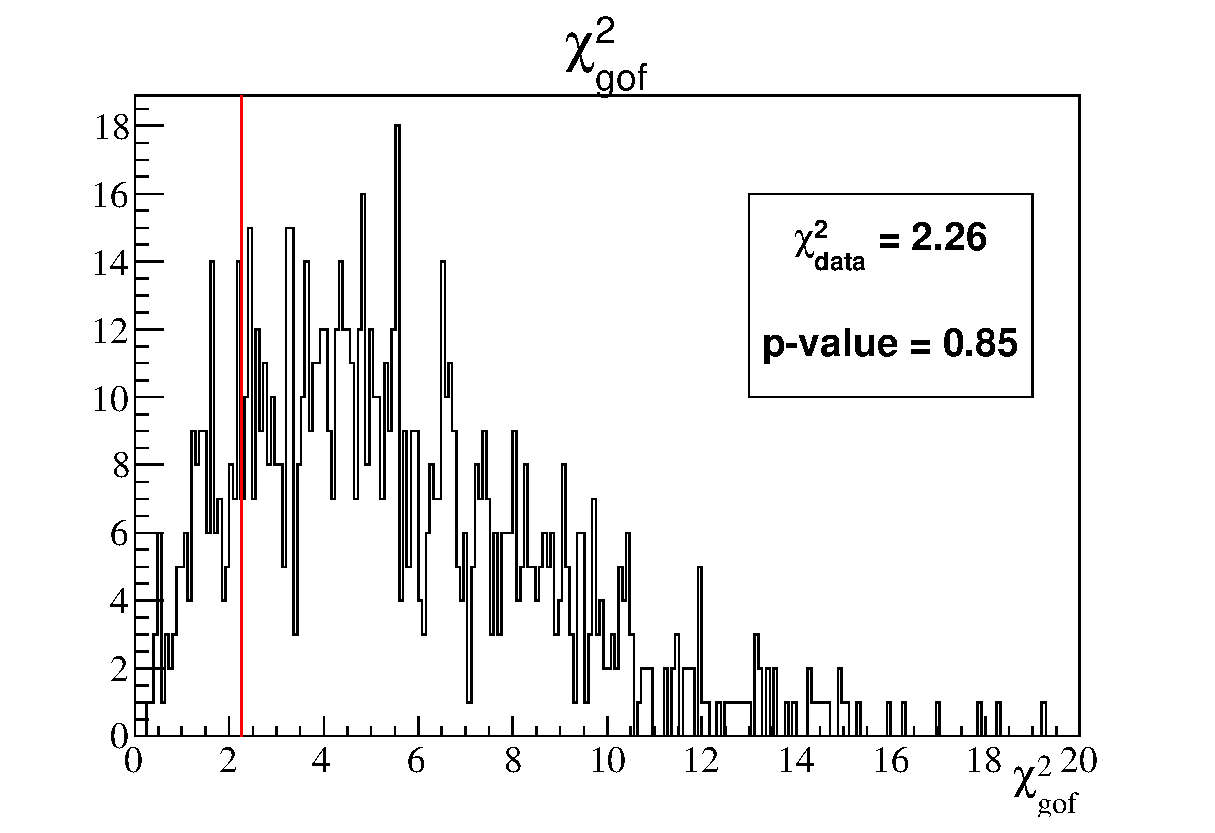
\includegraphics[width=30pc]{./images/results/data_ih_1st_gof_new.eps}
\caption {
  Distribution of $\chi^2_{gof}$, the goodness-of-fit (gof) $\chi^2$, 
  from 1k toy MC experiments generated at the Run 1+2+3 joint 3-flavour analysis best-fit oscillation point
  with Inverted Hierarchy.
  The $\chi^2_{gof}$ value for the Run 1+2+3 data ($\chi^2_{data}$) is highlighted.
  All $\chi^2_{gof}$ values were computed 
  using the 5 (single $\mu$-like ring) + 3 (single e-like ring) 
  reconstructed energy binning scheme described in Sec.\ \ref{sec:goodness_of_fit}.
}
\label{fig:run123_gofchisq_ih}
\end{minipage}

\vfill
\vspace*{0.7cm}

\begin{minipage}[t]{0.46\linewidth}
\center
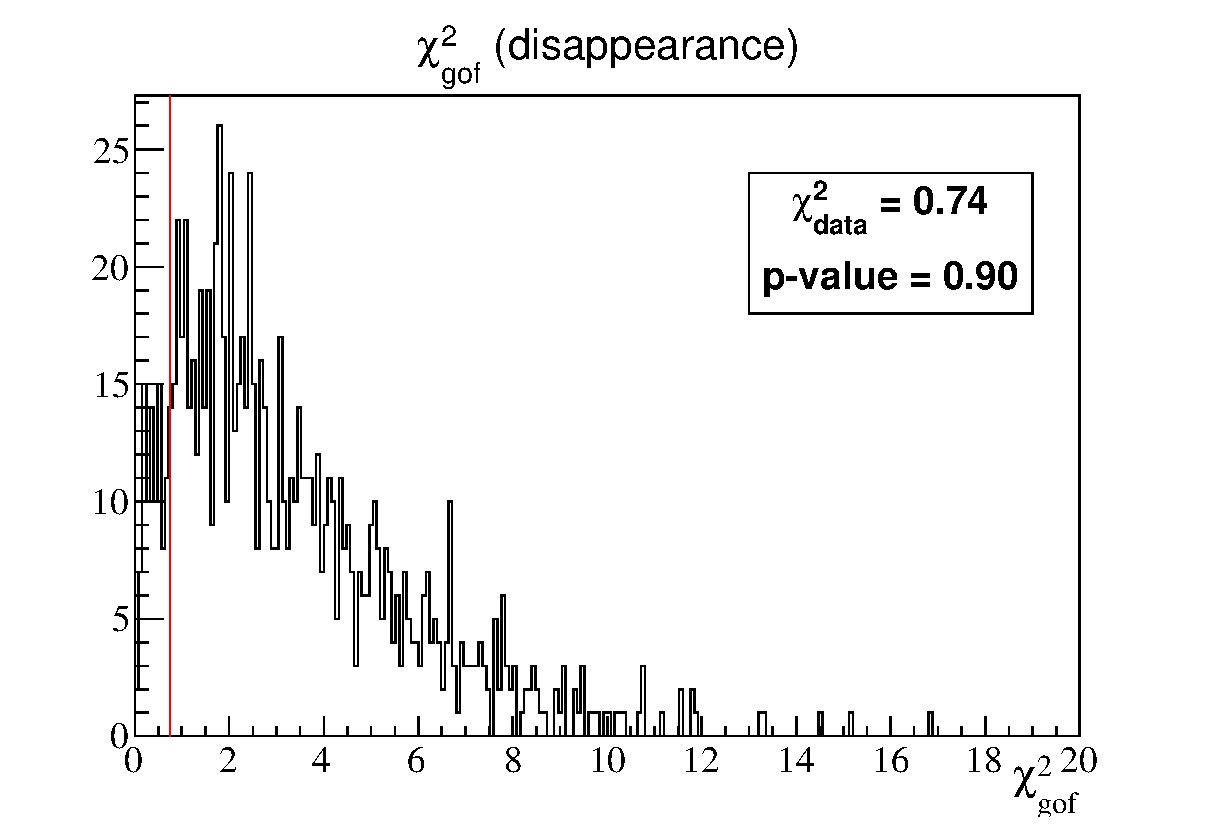
\includegraphics[width=18pc]{./images/results/data_ih_1st_gof_disap_new.eps}
\caption {
  Distribution of $\chi^2_{gof}$
  from 1k toy MC experiments generated at the Run 1+2+3 stand-alone 3-flavour $\nu_{\mu}$ disappearance analysis 
  best-fit oscillation point with Inverted Hierarchy.
  The $\chi^2_{gof}$ value for the Run 1+2+3 data ($\chi^2_{data}$) is highlighted.
  All $\chi^2_{gof}$ values were computed 
  using the 5 (single $\mu$-like ring) 
  reconstructed energy binning scheme described in Sec.\ \ref{sec:goodness_of_fit}.
}
\label{fig:run123_gofchisq_disapp_ih}
\end{minipage}
\hspace{0.03\linewidth}
\begin{minipage}[t]{0.46\linewidth}
\center
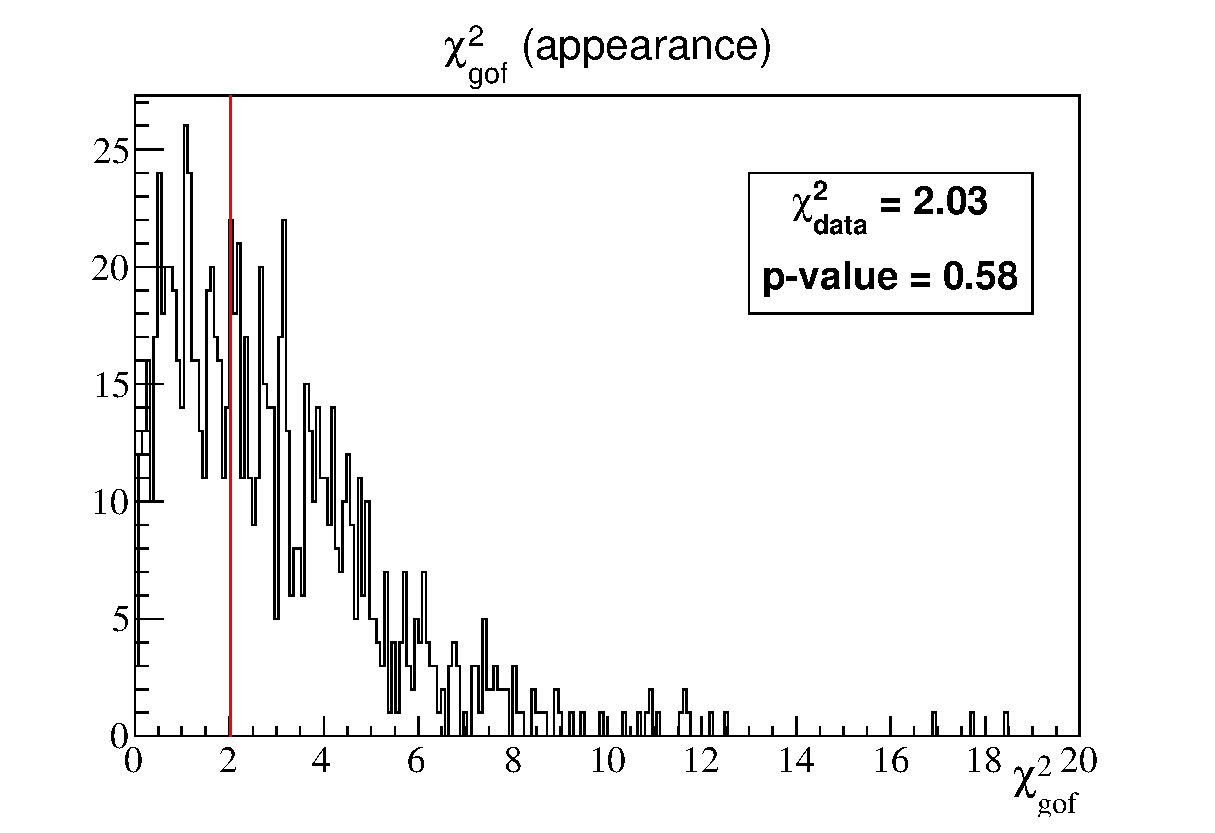
\includegraphics[width=18pc]{./images/results/data_ih_1st_gof_app_new.eps}
\caption {
  Distribution of $\chi^2_{gof}$
  from 1k toy MC experiments generated at the Run 1+2+3 stand-alone 3-flavour $\nu_{e}$ appearance analysis 
  best-fit oscillation point with Inverted Hierarchy.
  The $\chi^2_{gof}$ value for the Run 1+2+3 data ($\chi^2_{data}$) is highlighted.
  All $\chi^2_{gof}$ values were computed 
  using the 3 (single e-like ring) 
  reconstructed energy binning scheme  as described in Sec.\ \ref{sec:goodness_of_fit}.
}
\label{fig:run123_gofchisq_app_ih}
\end{minipage}

\end{figure*}




%...........................................................
%
% Best-fit spectra from the joint-analysis and stand-alone analyses 
% Binning used in the fit
%

\begin{figure*}[htb]

\begin{minipage}[t]{0.98\linewidth}
\center
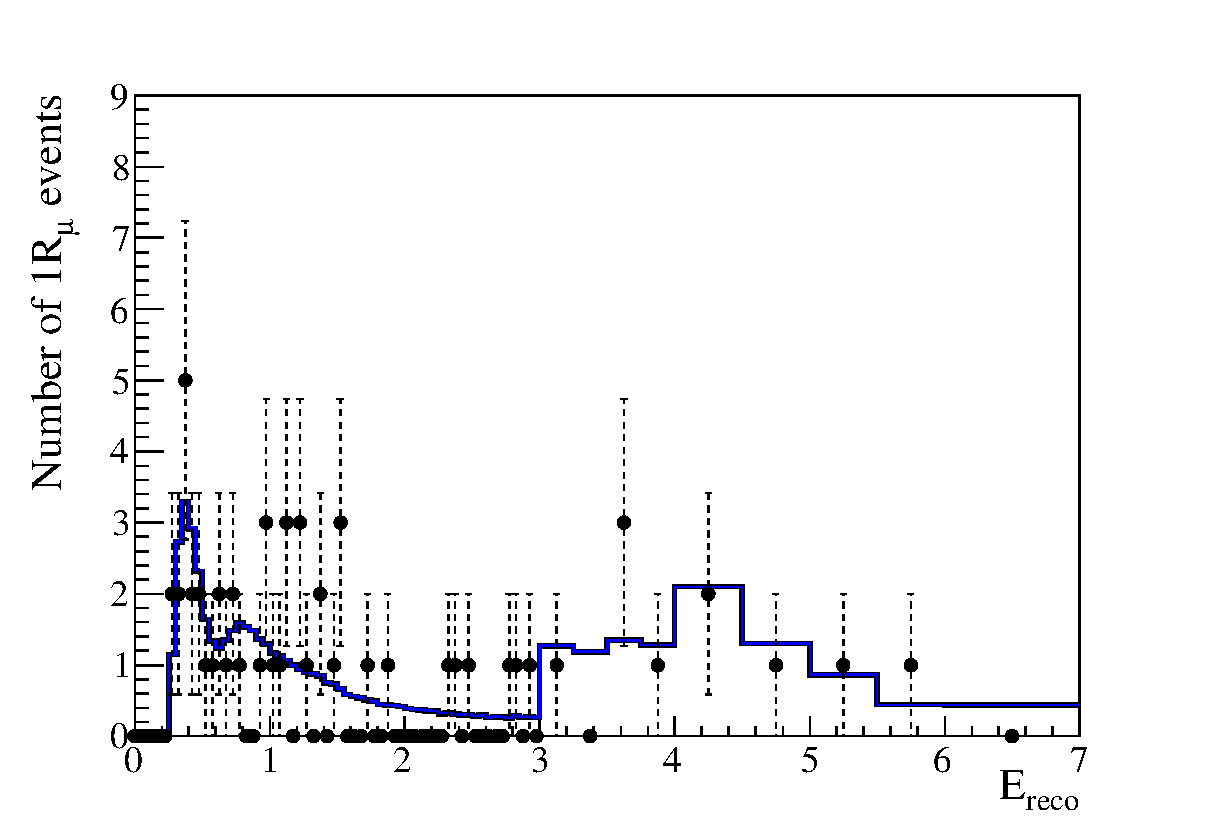
\includegraphics[width=28pc]{./images/results/data_nh_1st_1Rmu.eps}
\caption {
  Run 1+2+3 best-fit single $\mu$-like ring event reconstructed energy spectrum for the fit with Normal Hierarchy
  (black: joint 3-flavour oscillation analysis, blue: stand-alone $\nu_{\mu}$ disappearance analysis).
  The distributions are shown with the binning used in the fit.
}
\label{fig:run123_1Rmu_bestfit_spectrum_nh}
\end{minipage}

\vfill
\vspace*{0.7cm}

\begin{minipage}[t]{0.98\linewidth}
\center
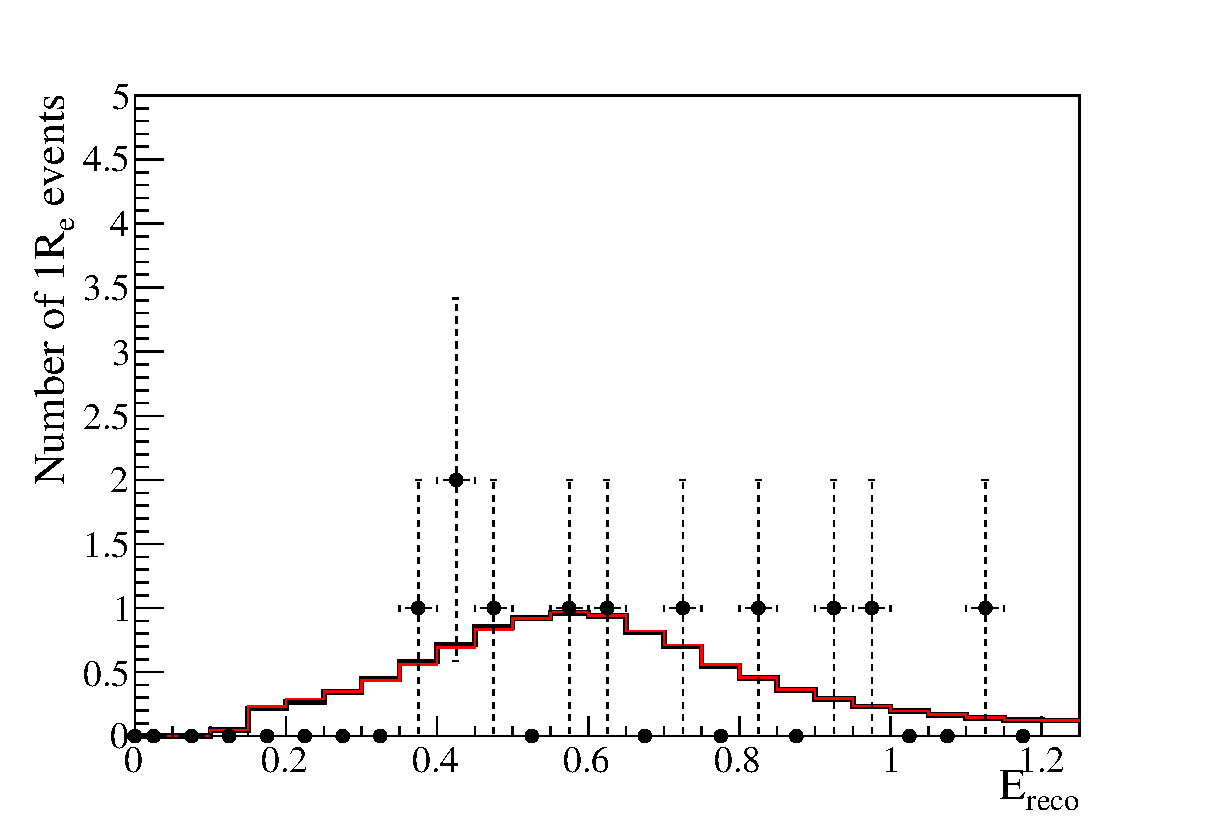
\includegraphics[width=28pc]{./images//results/data_nh_1st_1Re.eps}
\caption {
  Run 1+2+3 best-fit single e-like ring event reconstructed energy spectrum for the fit with Normal Hierarchy
  (black: joint 3-flavour oscillation analysis, red: stand-alone $\nu_{e}$ disappearance analysis).
  The distributions are shown with the binning used in the fit.
}
\label{fig:run123_1Re_bestfit_spectrum_nh}
\end{minipage}

\end{figure*}

\begin{figure*}[htb]

\begin{minipage}[t]{0.98\linewidth}
\center
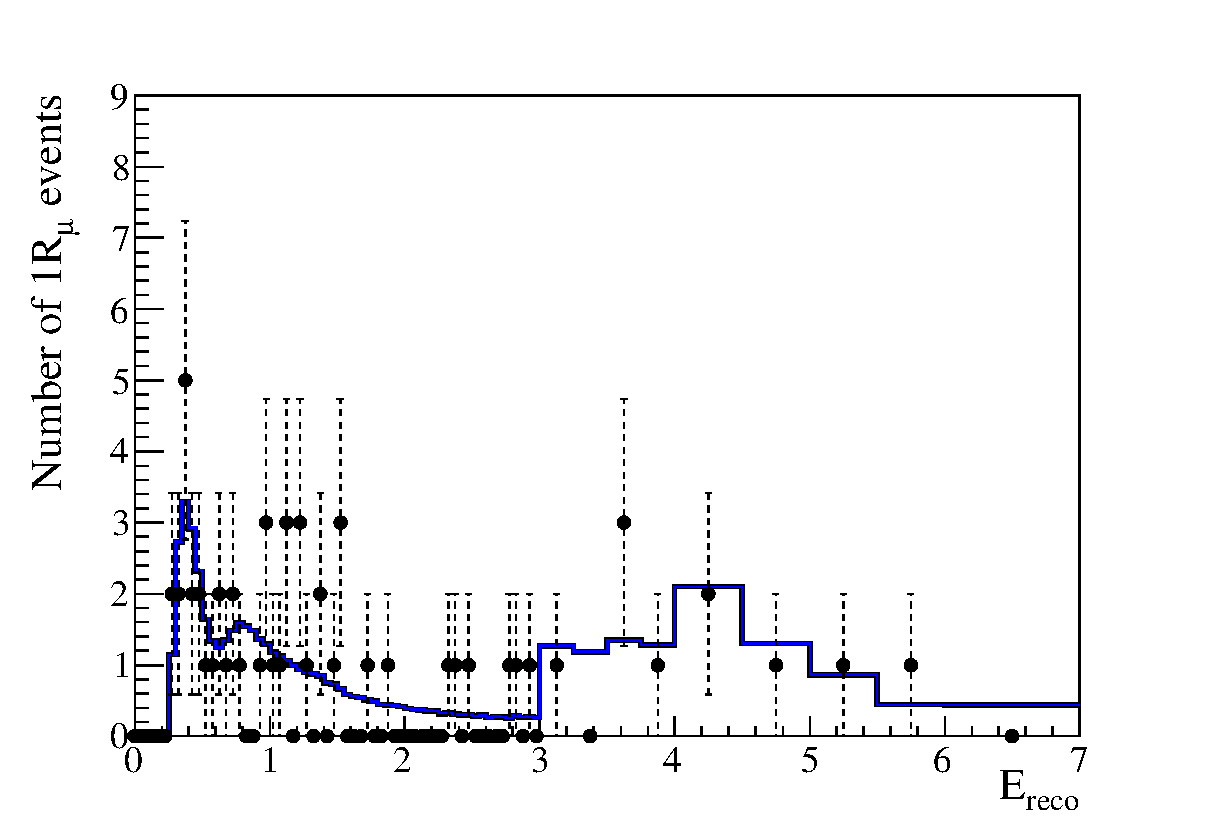
\includegraphics[width=28pc]{./images//results/data_ih_1st_1Rmu.eps}
\caption {
  Run 1+2+3 best-fit single $\mu$-like ring event reconstructed energy spectrum for the fit with Inverted Hierarchy
  (black: joint 3-flavour oscillation analysis, blue: stand-alone $\nu_{\mu}$ disappearance analysis).
  The distributions are shown with the binning used in the fit.
}
\label{fig:run123_1Rmu_bestfit_spectrum_ih}
\end{minipage}

\vfill
\vspace*{0.7cm}

\begin{minipage}[t]{0.98\linewidth}
\center
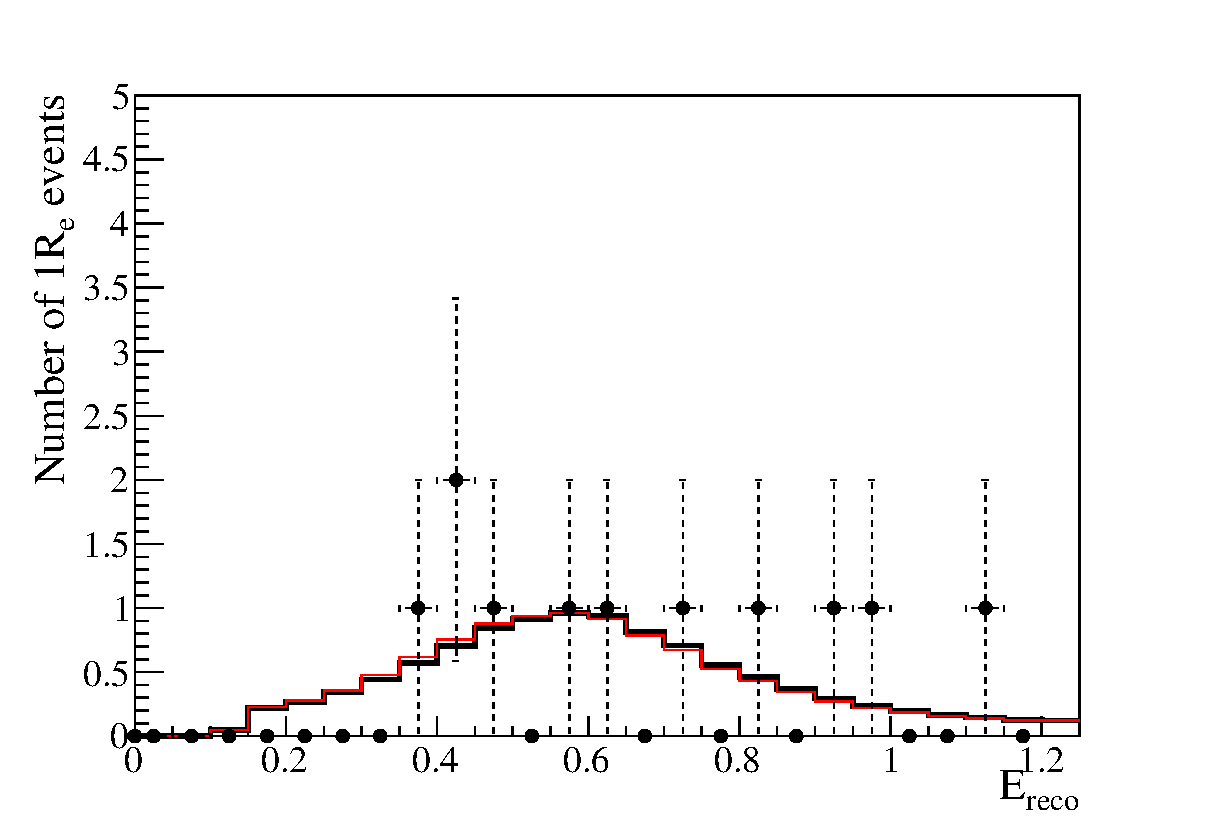
\includegraphics[width=28pc]{./images//results/data_ih_1st_1Re.eps}
\caption {
  Run 1+2+3 best-fit single e-like ring event reconstructed energy spectrum for the fit with inverted Hierarchy
  (black: joint 3-flavour oscillation analysis, red: stand-alone $\nu_{e}$ disappearance analysis).
  The distributions are shown with the binning used in the fit.
}
\label{fig:run123_1Re_bestfit_spectrum_ih}
\end{minipage}

\end{figure*}


%...........................................................
%
% Best-fit spectra from the joint-analysis and stand-alone analyses 
% Coarse binning.
%

\begin{figure*}[htb]

\begin{minipage}[t]{0.98\linewidth}
\center
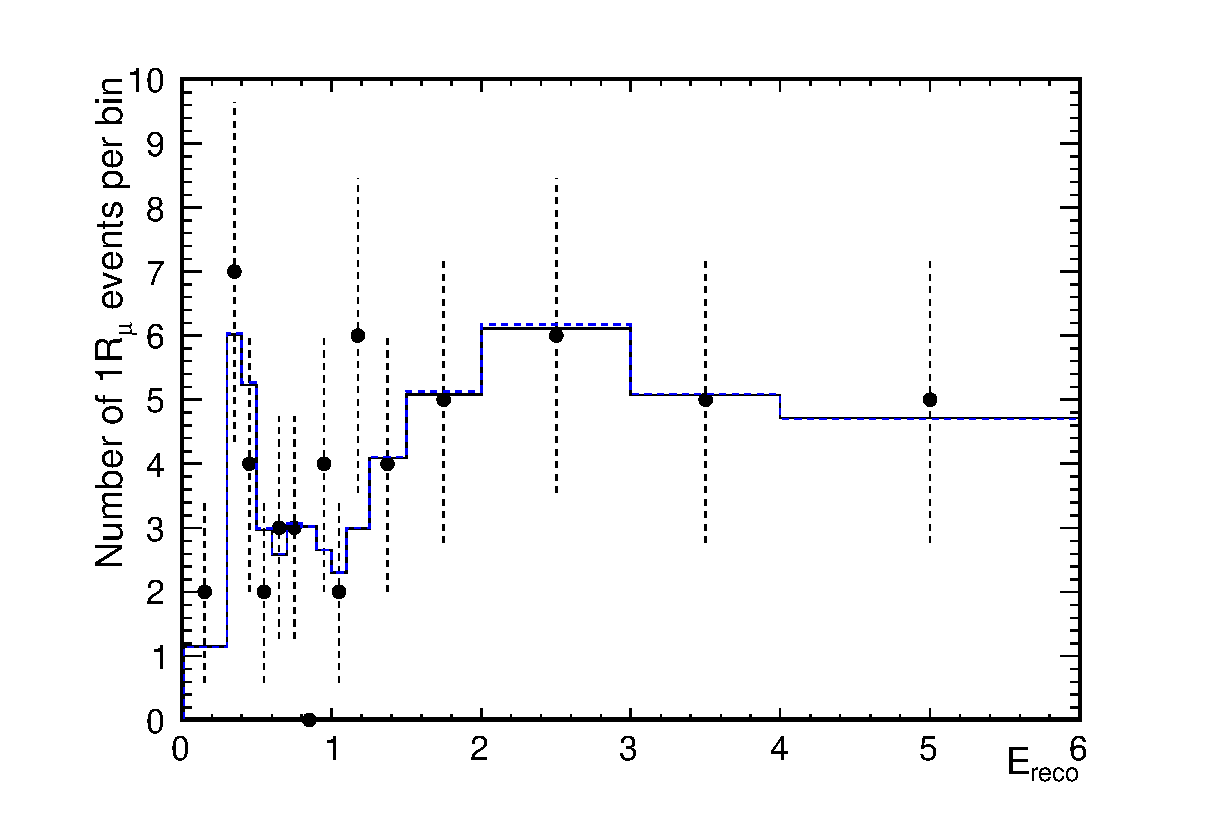
\includegraphics[width=28pc]{./images/results/bestfit_spectra_1Rmu_nh_coarse.eps}
\caption {
  Run 1+2+3 best-fit single $\mu$-like ring event reconstructed energy spectrum for the fit with Normal Hierarchy
  (black: joint 3-flavour oscillation analysis, blue: stand-alone $\nu_{\mu}$ disappearance analysis).
  The distributions are shown with the coarse binning defined in the main text.
}
\label{fig:run123_1Rmu_bestfit_spectrum_nh_coarse}
\end{minipage}

\vfill
\vspace*{0.7cm}

\begin{minipage}[t]{0.98\linewidth}
\center
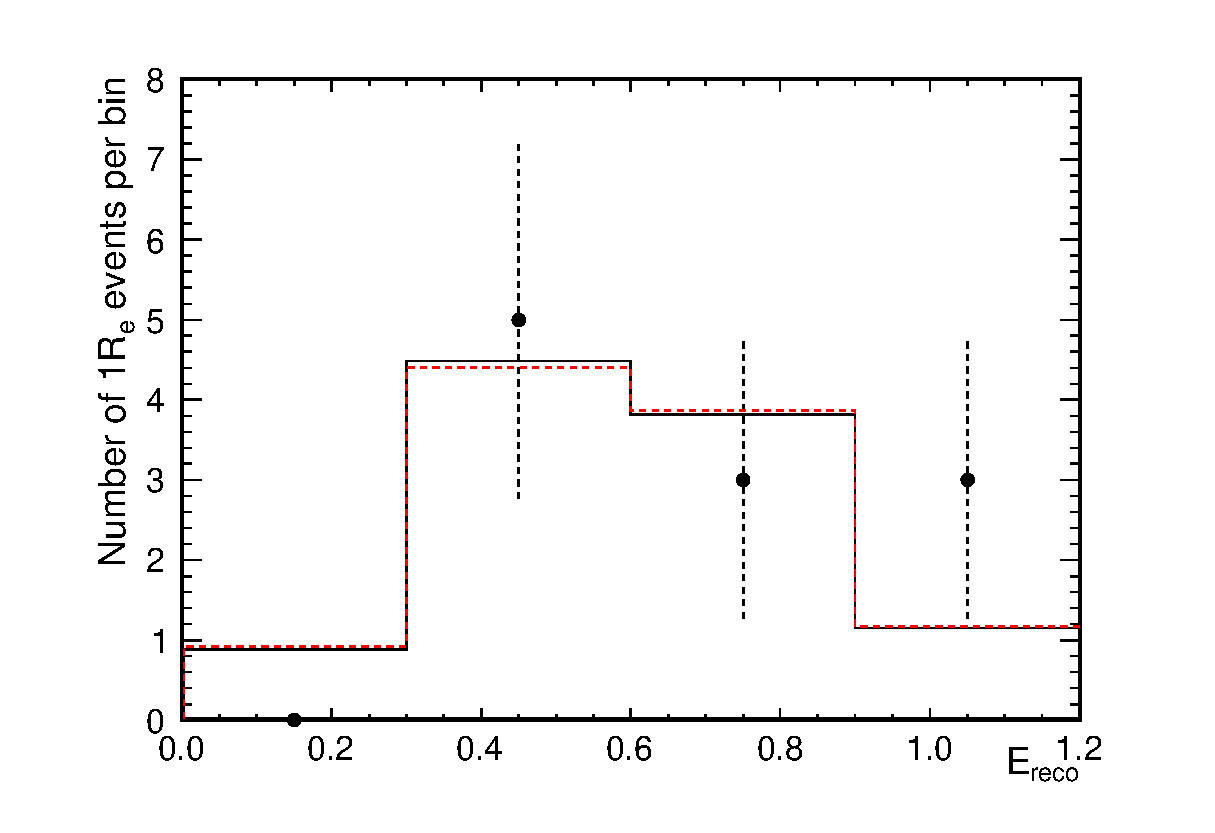
\includegraphics[width=28pc]{./images//results/bestfit_spectra_1Re_nh_coarse.eps}
\caption {
  Run 1+2+3 best-fit single e-like ring event reconstructed energy spectrum for the fit with Normal Hierarchy
  (black: joint 3-flavour oscillation analysis, red: stand-alone $\nu_{e}$ disappearance analysis).
  The distributions are shown with the coarse binning defined in the main text.
}
\label{fig:run123_1Re_bestfit_spectrum_nh_coarse}
\end{minipage}

\end{figure*}

\begin{figure*}[htb]

\begin{minipage}[t]{0.98\linewidth}
\center
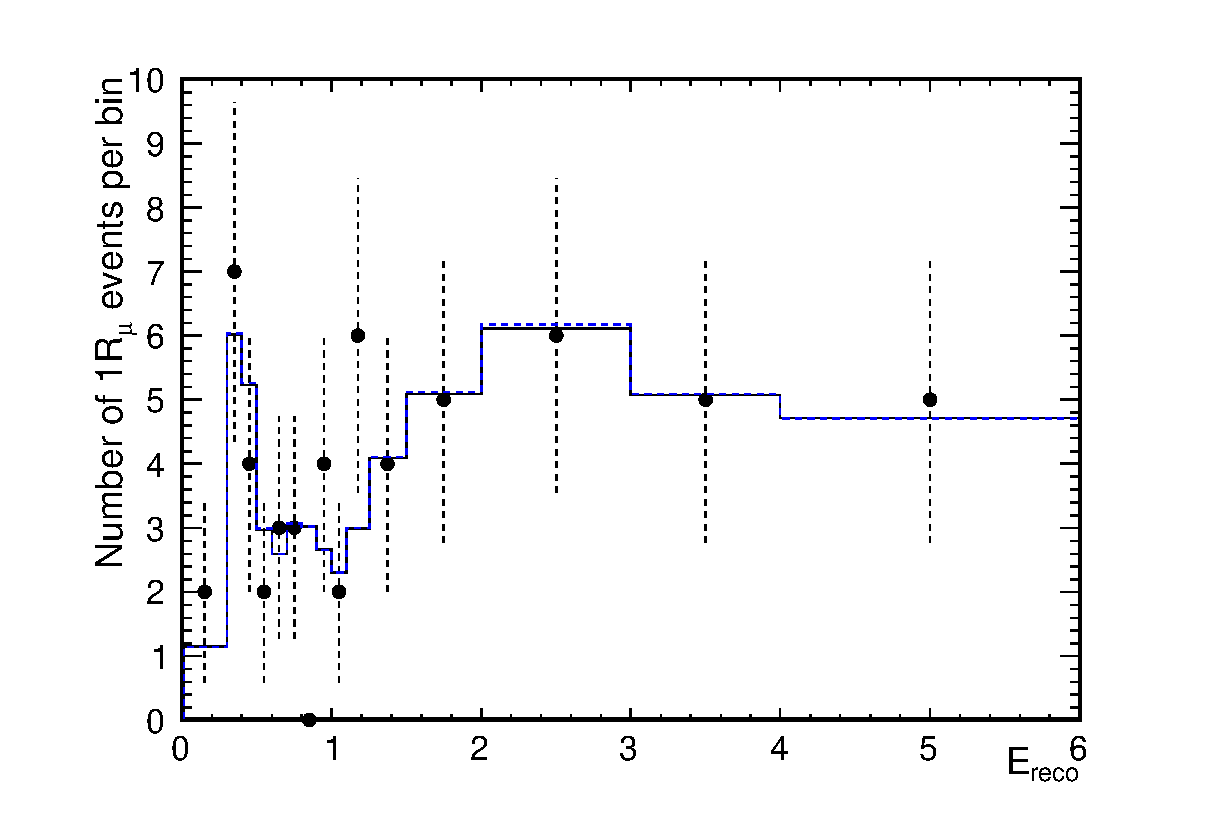
\includegraphics[width=28pc]{./images//results/bestfit_spectra_1Rmu_ih_coarse.eps}
\caption {
  Run 1+2+3 best-fit single $\mu$-like ring event reconstructed energy spectrum for the fit with Inverted Hierarchy
  (black: joint 3-flavour oscillation analysis, blue: stand-alone $\nu_{\mu}$ disappearance analysis).
  The distributions are shown with the coarse binning defined in the main text.
}
\label{fig:run123_1Rmu_bestfit_spectrum_ih_coarse}
\end{minipage}

\vfill
\vspace*{0.7cm}

\begin{minipage}[t]{0.98\linewidth}
\center
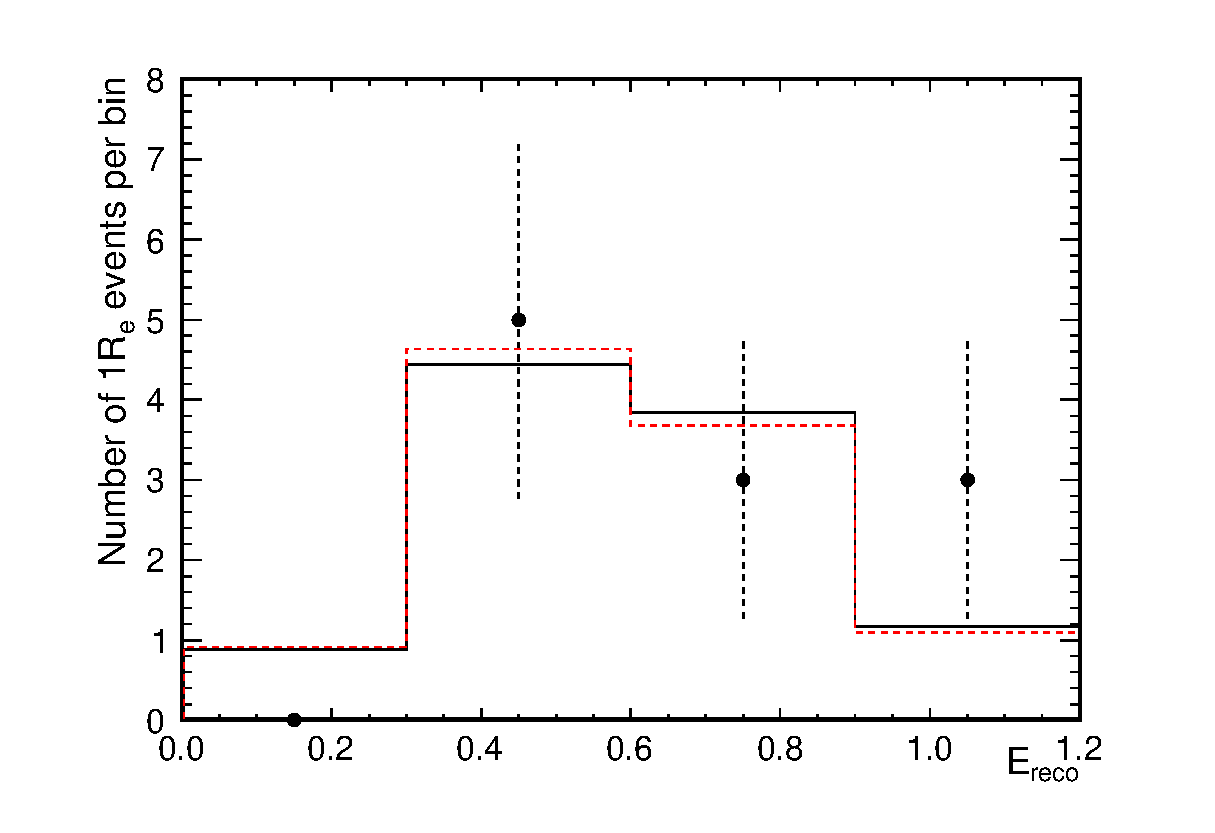
\includegraphics[width=28pc]{./images//results/bestfit_spectra_1Re_ih_coarse.eps}
\caption {
  Run 1+2+3 best-fit single e-like ring event reconstructed energy spectrum for the fit with inverted Hierarchy
  (black: joint 3-flavour oscillation analysis, red: stand-alone $\nu_{e}$ disappearance analysis).
  The distributions are shown with the coarse binning defined in the main text.
}
\label{fig:run123_1Re_bestfit_spectrum_ih_coarse}
\end{minipage}

\end{figure*}


%...........................................................
%
% Ratio of the best-fit spectra from the joint-analysis over the
% best-fit spectra from the stand-alone analyses.
% Binning used in the fit
%

\begin{figure*}[htb]

\begin{minipage}[t]{0.98\linewidth}
\center
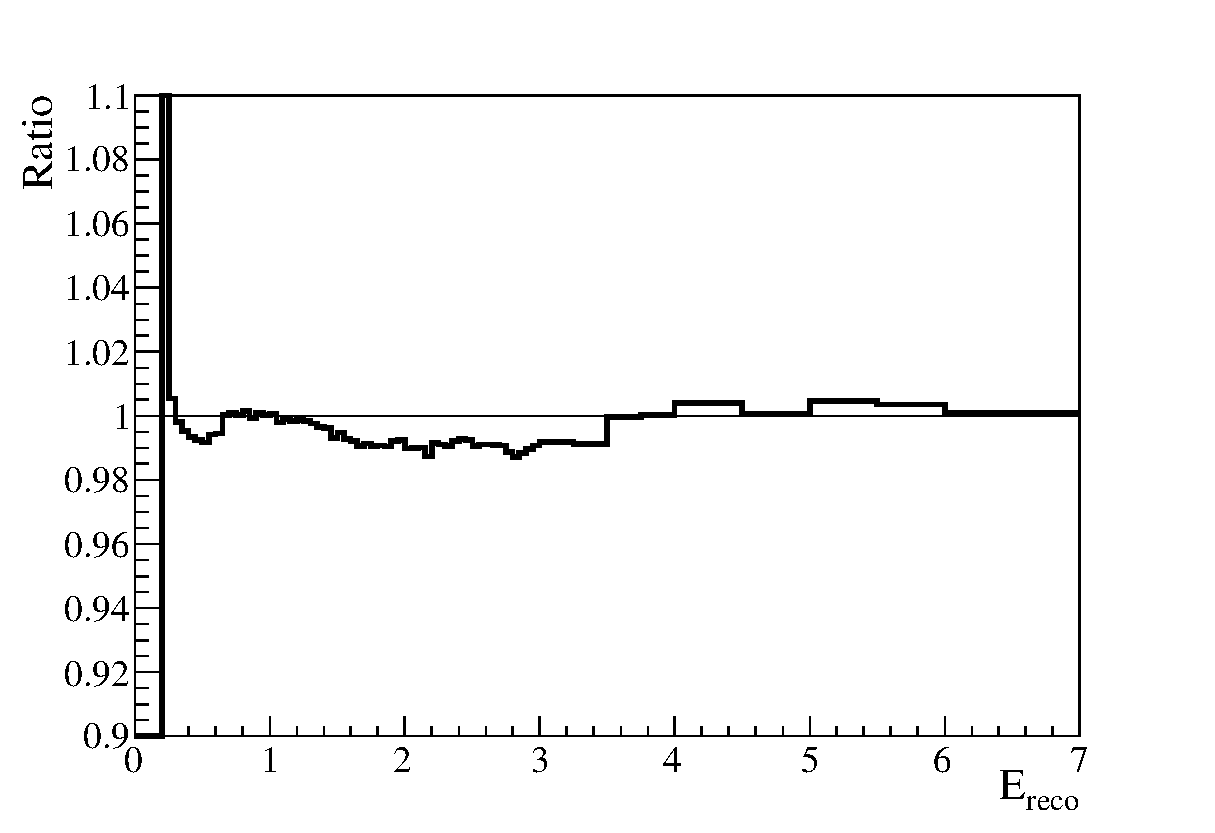
\includegraphics[width=28pc]{./images/results/Ratio_data_nh_1st_1Rmu.eps}
\caption {
  Ratio of the Run 1+2+3 best-fit single $\mu$-like ring event reconstructed energy spectra
  obtained from the joint 3-flavour oscillation and the stand-alone $\nu_{\mu}$ disappearance analyses
  (joint / stand-alone) with Normal Hierarchy.
  The distributions are shown with the binning used in the fit.
}
\label{fig:run123_1Rmu_bestfit_spectrum_ratio_nh}
\end{minipage}

\vfill
\vspace*{0.7cm}

\begin{minipage}[t]{0.98\linewidth}
\center
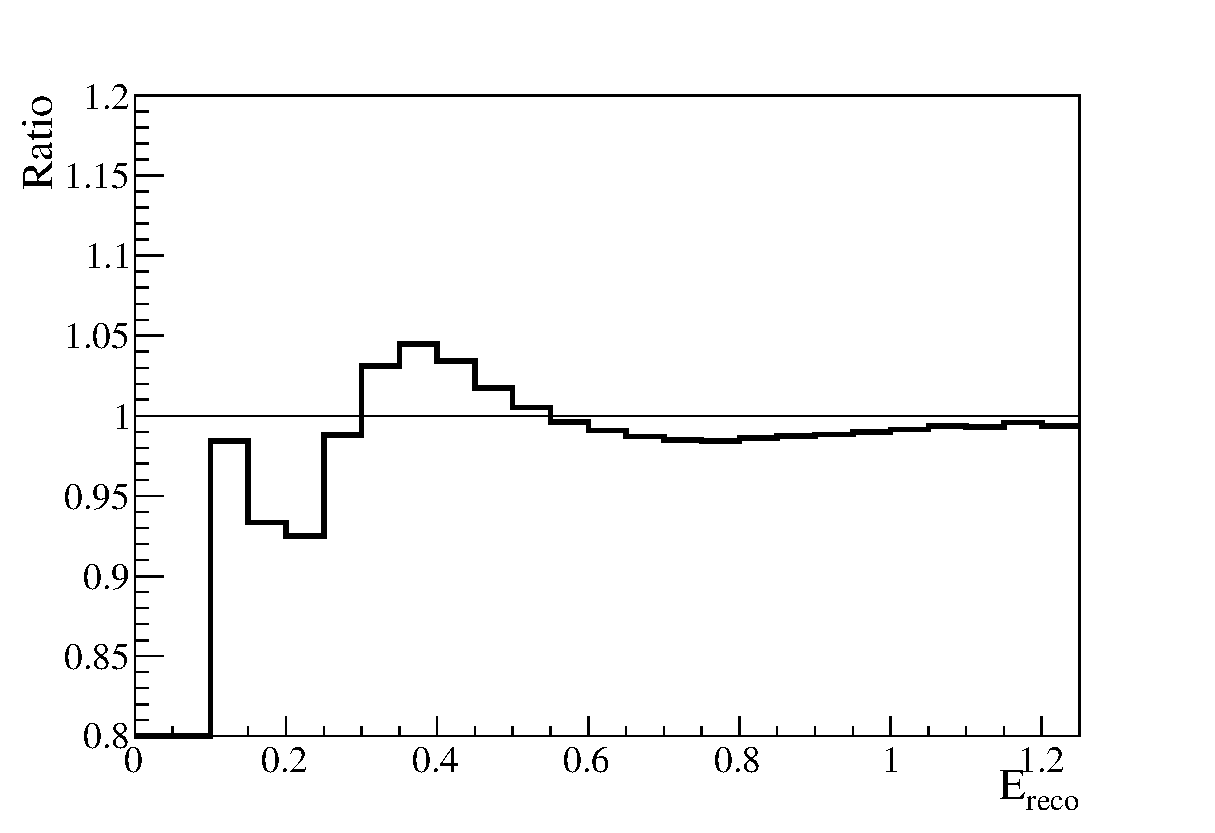
\includegraphics[width=28pc]{./images/results/Ratio_data_nh_1st_1Re.eps}
\caption {
  Ratio of the Run 1+2+3 best-fit single e-like ring event reconstructed energy spectra
  obtained from the joint 3-flavour oscillation and the stand-alone $\nu_{e}$ appearance analyses.
  (joint / stand-alone) with Normal Hierarchy.
  The distributions are shown with the binning used in the fit.
}
\label{fig:run123_1Re_bestfit_spectrum_ratio_nh}
\end{minipage}

\end{figure*}

\begin{figure*}[htb]

\begin{minipage}[t]{0.98\linewidth}
\center
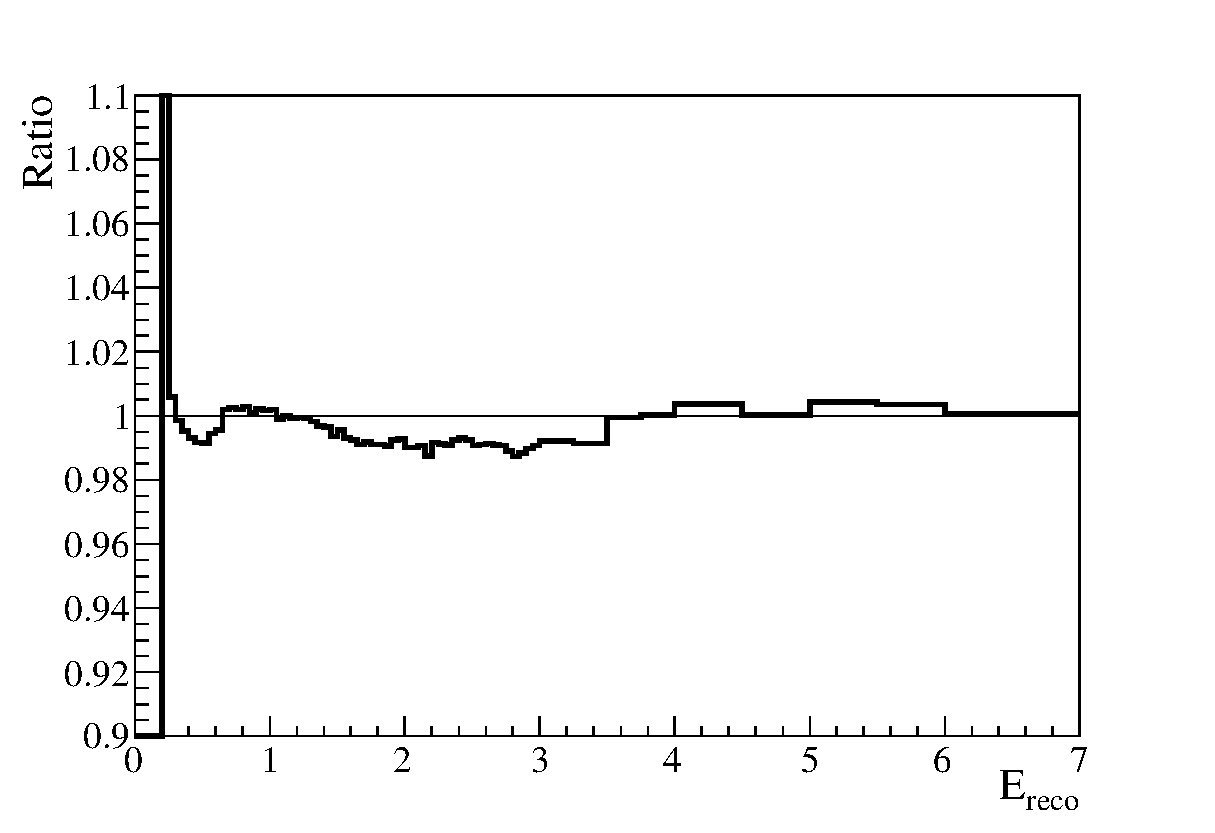
\includegraphics[width=28pc]{./images/results/Ratio_data_ih_1st_1Rmu.eps}
\caption {
  Ratio of the Run 1+2+3 best-fit single $\mu$-like ring event reconstructed energy spectra
  obtained from the joint 3-flavour oscillation and the stand-alone $\nu_{\mu}$ disappearance analyses
  (joint / stand-alone) with Inverted Hierarchy.
  The distributions are shown with the binning used in the fit.
}
\label{fig:run123_1Rmu_bestfit_spectrum_ratio_ih}
\end{minipage}

\vfill
\vspace*{0.7cm}

\begin{minipage}[t]{0.98\linewidth}
\center
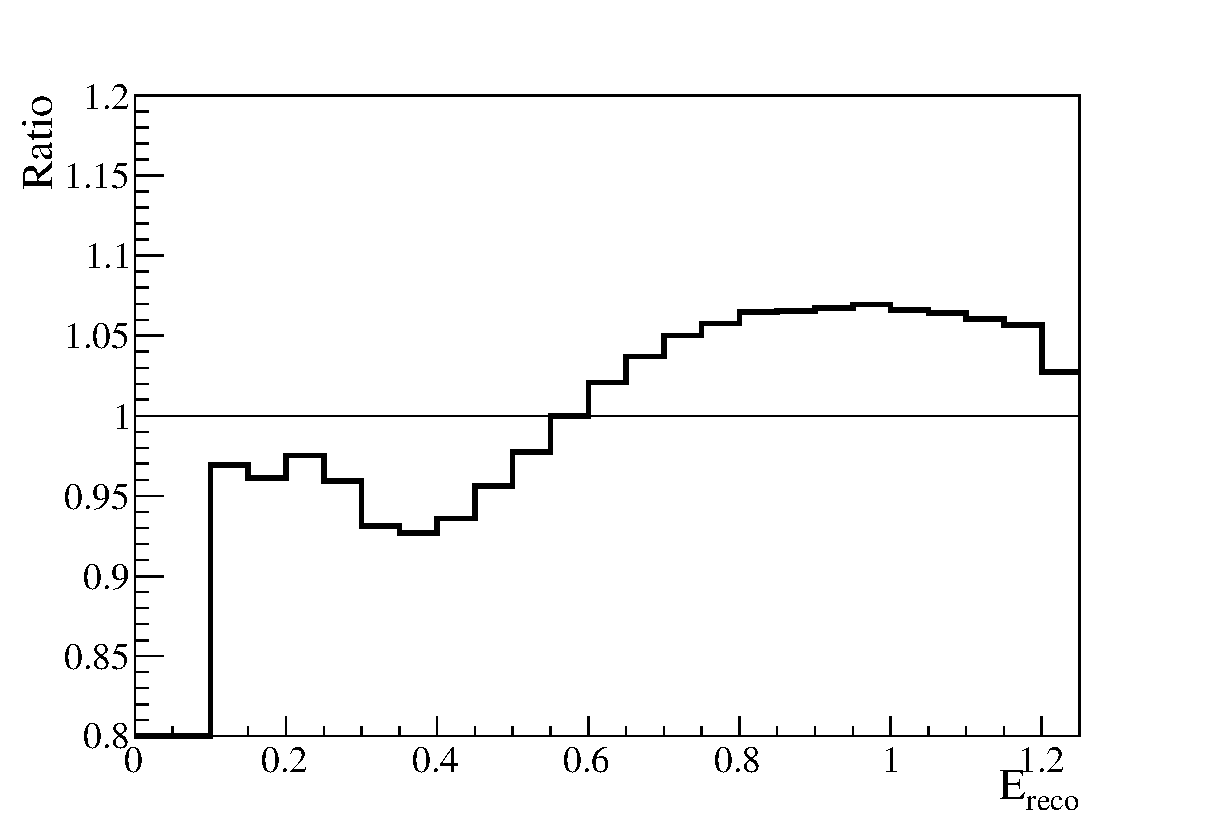
\includegraphics[width=28pc]{./images/results/Ratio_data_ih_1st_1Re.eps}
\caption {
  Ratio of the Run 1+2+3 best-fit single e-like ring event reconstructed energy spectra
  obtained from the joint 3-flavour oscillation and the stand-alone $\nu_{e}$ appearance analyses.
  (joint / stand-alone) with Inverted Hierarchy.
  The distributions are shown with the binning used in the fit.
}
\label{fig:run123_1Re_bestfit_spectrum_ratio_ih}
\end{minipage}

\end{figure*}


%...........................................................
%
% marginalized (1D) delta\chisq distributions
%

\begin{figure*}[htb]

\begin{minipage}[t]{0.45\linewidth}
\center
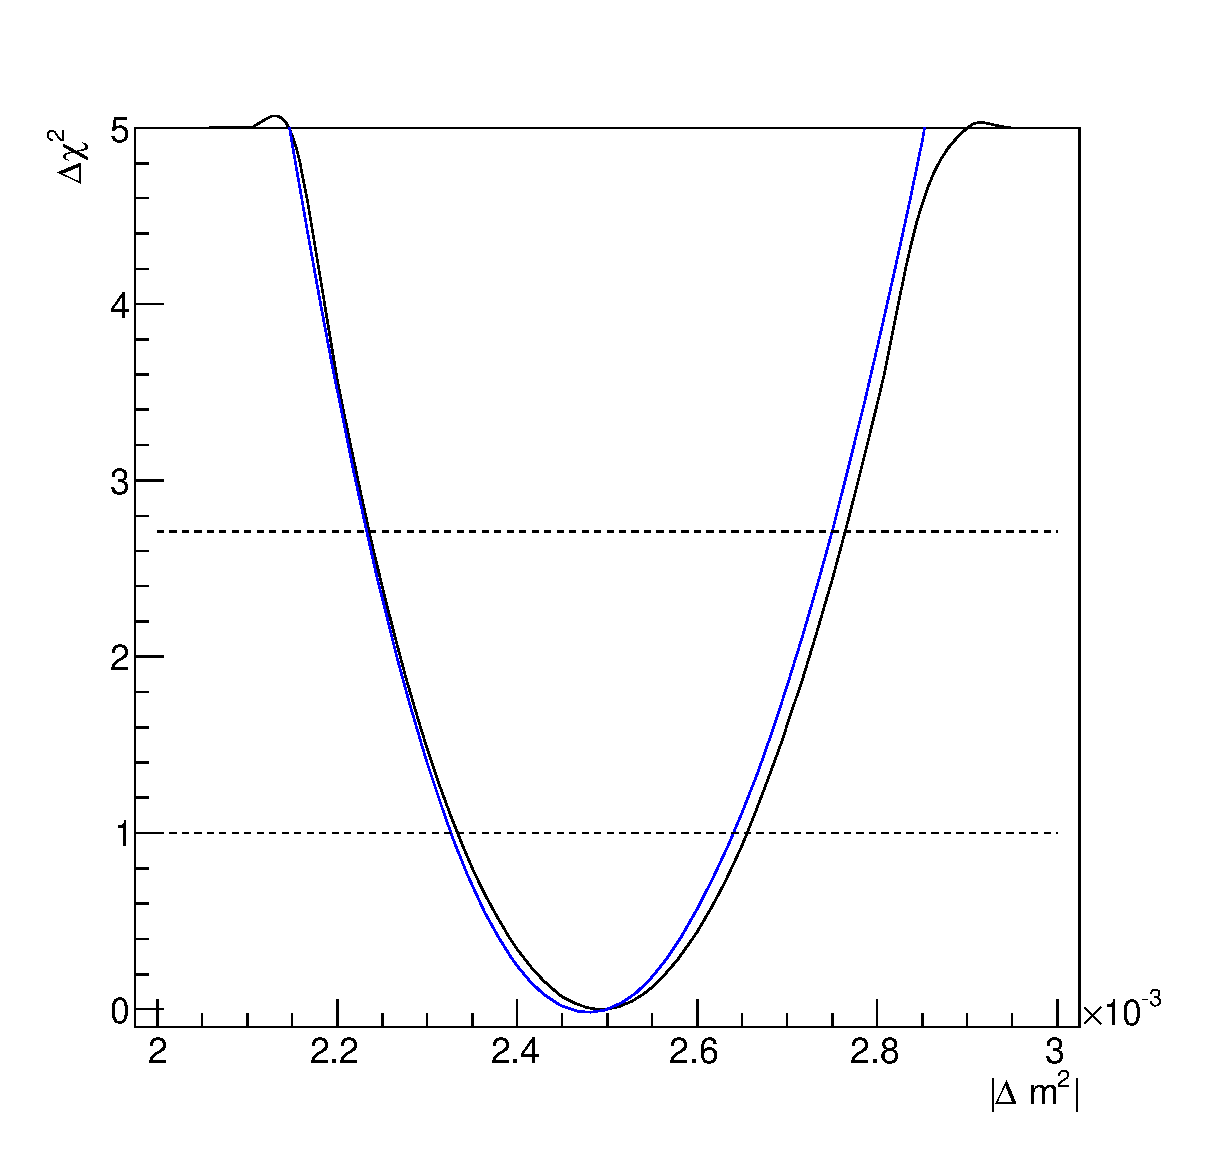
\includegraphics[width=18pc]{./images/results/data_chisq_dm23sq_global_min_new.eps}
\caption {
  $\Delta\chi^2$ as function of $|\Delta m^{2}|$ from the analysis of the Run 1+2+3 dataset
  comparing the joint analysis (black) with the stand-alone $\nu_{\mu}$ disappearance (blue)
  for Normal Hierarchy. 
  At each point, $\chi^2$ was minimized with respect to
  all oscillation parameters not shown (and not considered to be fixed)
  and all relevant nuisance parameters.
}
\label{fig:run123_dchisq_Dmsq_nh}
\end{minipage}
\hspace{0.04\linewidth}
\begin{minipage}[t]{0.45\linewidth}
\center
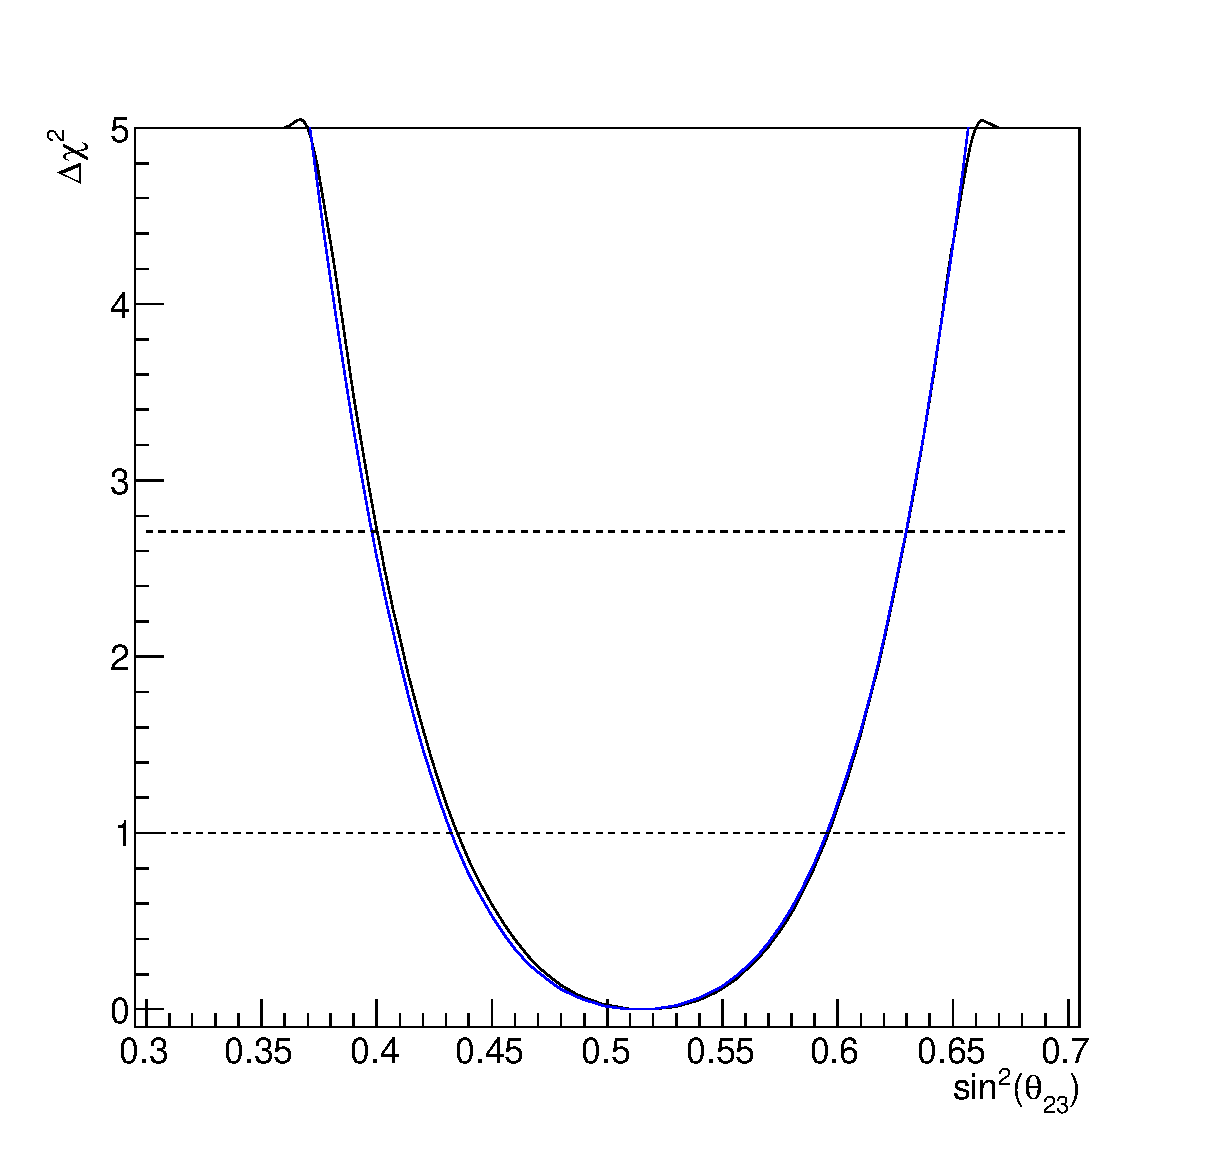
\includegraphics[width=18pc]{./images/results/data_chisq_theta23_global_min_new.eps}
\caption {
  $\Delta\chi^2$ as function of $sin^{2}\theta_{23}$ from the analysis of the Run 1+2+3 dataset
   comparing the joint analysis (black) with the stand-alone $\nu_{\mu}$ disappearance (blue)
     for Normal Hierarchy. 	
  At each point, $\chi^2$ was minimized with respect to
  all oscillation parameters not shown (and not considered to be fixed)
  and all relevant nuisance parameters.
}
\label{fig:run123_dchisq_sinsqtheta23_nh}
\end{minipage}

\vfill
\vspace*{0.7cm}

\begin{minipage}[t]{0.45\linewidth}
\center
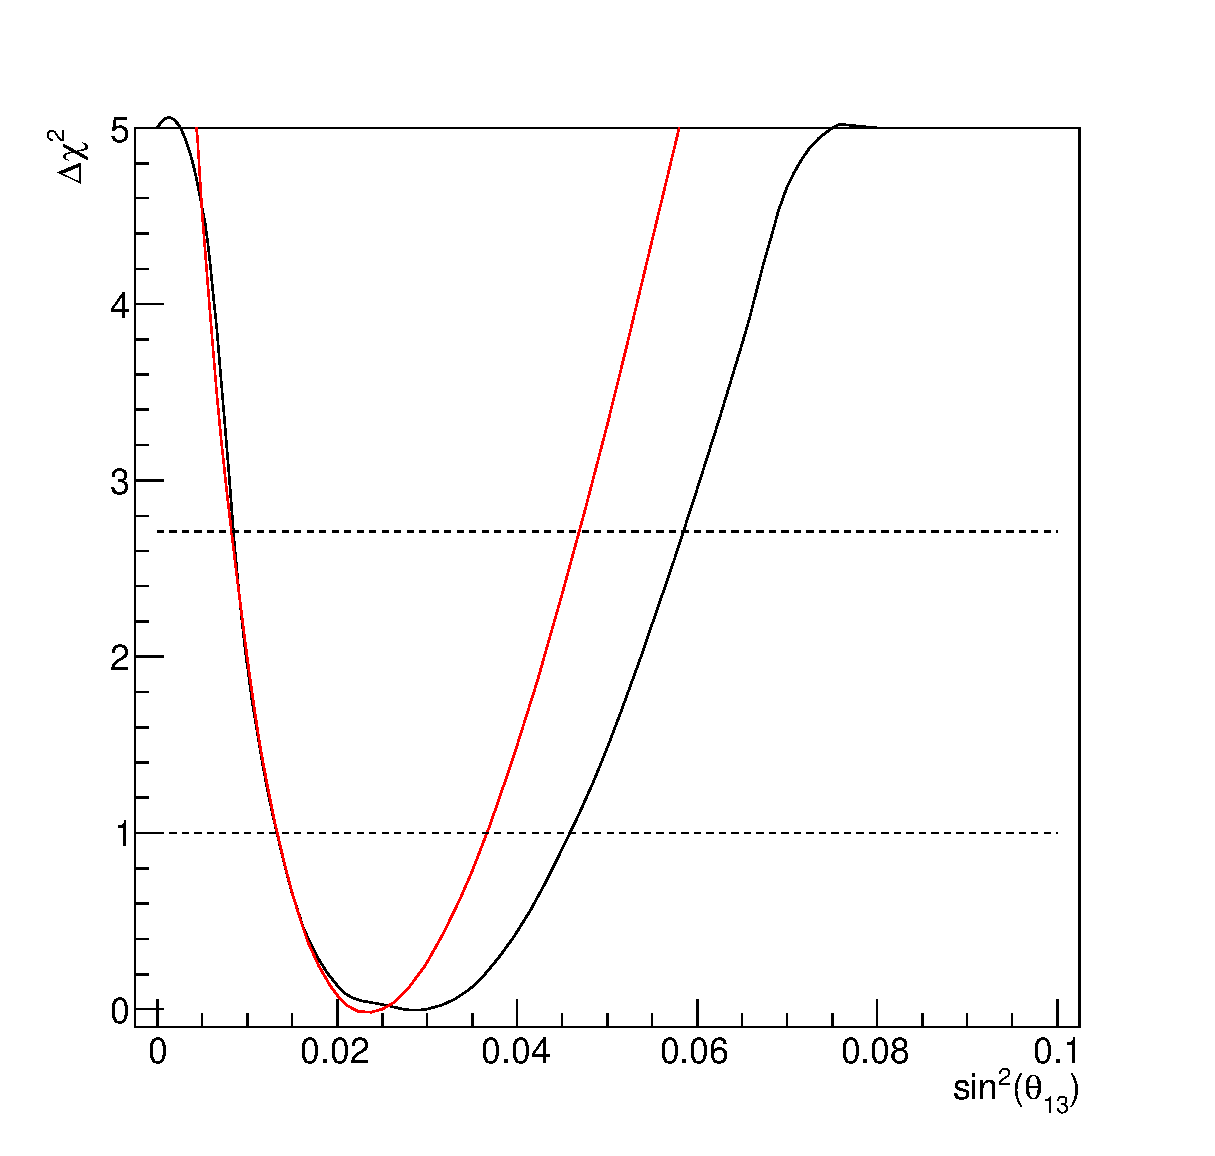
\includegraphics[width=18pc]{./images/results/data_chisq_theta13_global_min_new.eps}
\caption {
  $\Delta\chi^2$ as function of $sin^{2}\theta_{13}$ from the analysis of the Run 1+2+3 dataset
   comparing the joint analysis (black) with the stand-alone $\nu_{e}$ appearance (red)
     for Normal Hierarchy. 
  At each point, $\chi^2$ was minimized with respect to
  all oscillation parameters not shown (and not considered to be fixed)
  and all relevant nuisance parameters.
}
\label{fig:run123_dchisq_sinsqtheta13_nh}
\end{minipage}
\hspace{0.04\linewidth}
\begin{minipage}[t]{0.45\linewidth}
\center
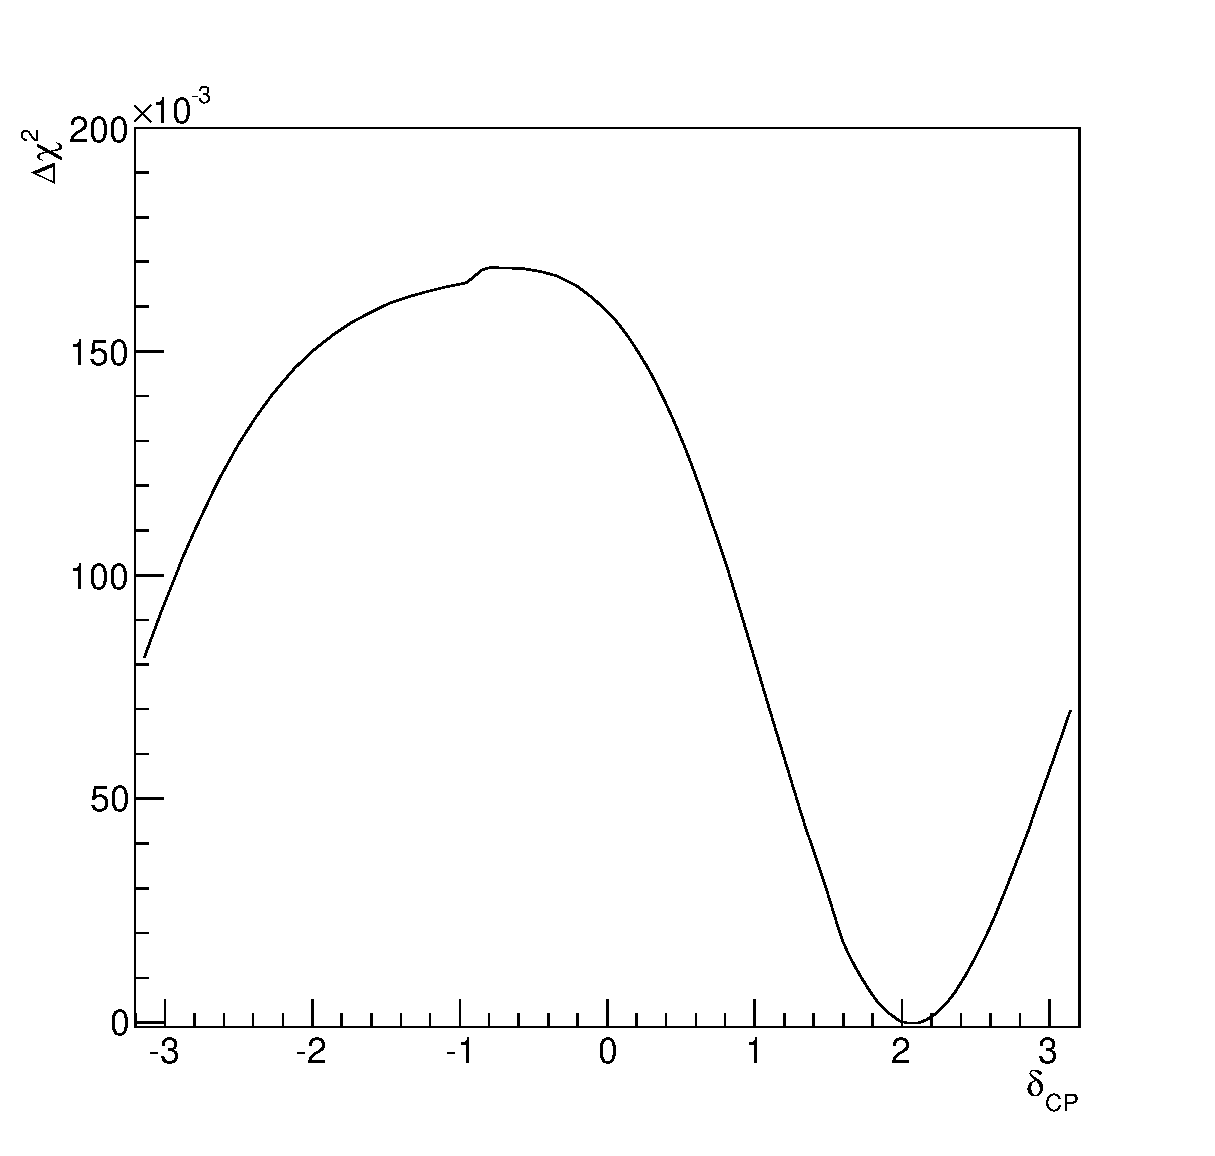
\includegraphics[width=18pc]{./images/results/data_chisq_deltacp_global_min_new.eps}
\caption {
  $\Delta\chi^2$ as function of $\delta_{CP}$ from the analysis of the Run 1+2+3 dataset  for Normal Hierarchy. 
  At each point, $\chi^2$ was minimized with respect to
  all oscillation parameters not shown (and not considered to be fixed)
  and all relevant nuisance parameters.
}
\label{fig:run123_dchisq_deltacp_nh}
\end{minipage}

\end{figure*}

%...........................................................
%
% contours 
% that can be compared with stand-alone analyses
% dmsq - sinsqtheta23, deltacp - sinsqtheta13
%

\begin{figure*}[htb]

\begin{minipage}[t]{0.98\linewidth}
\center
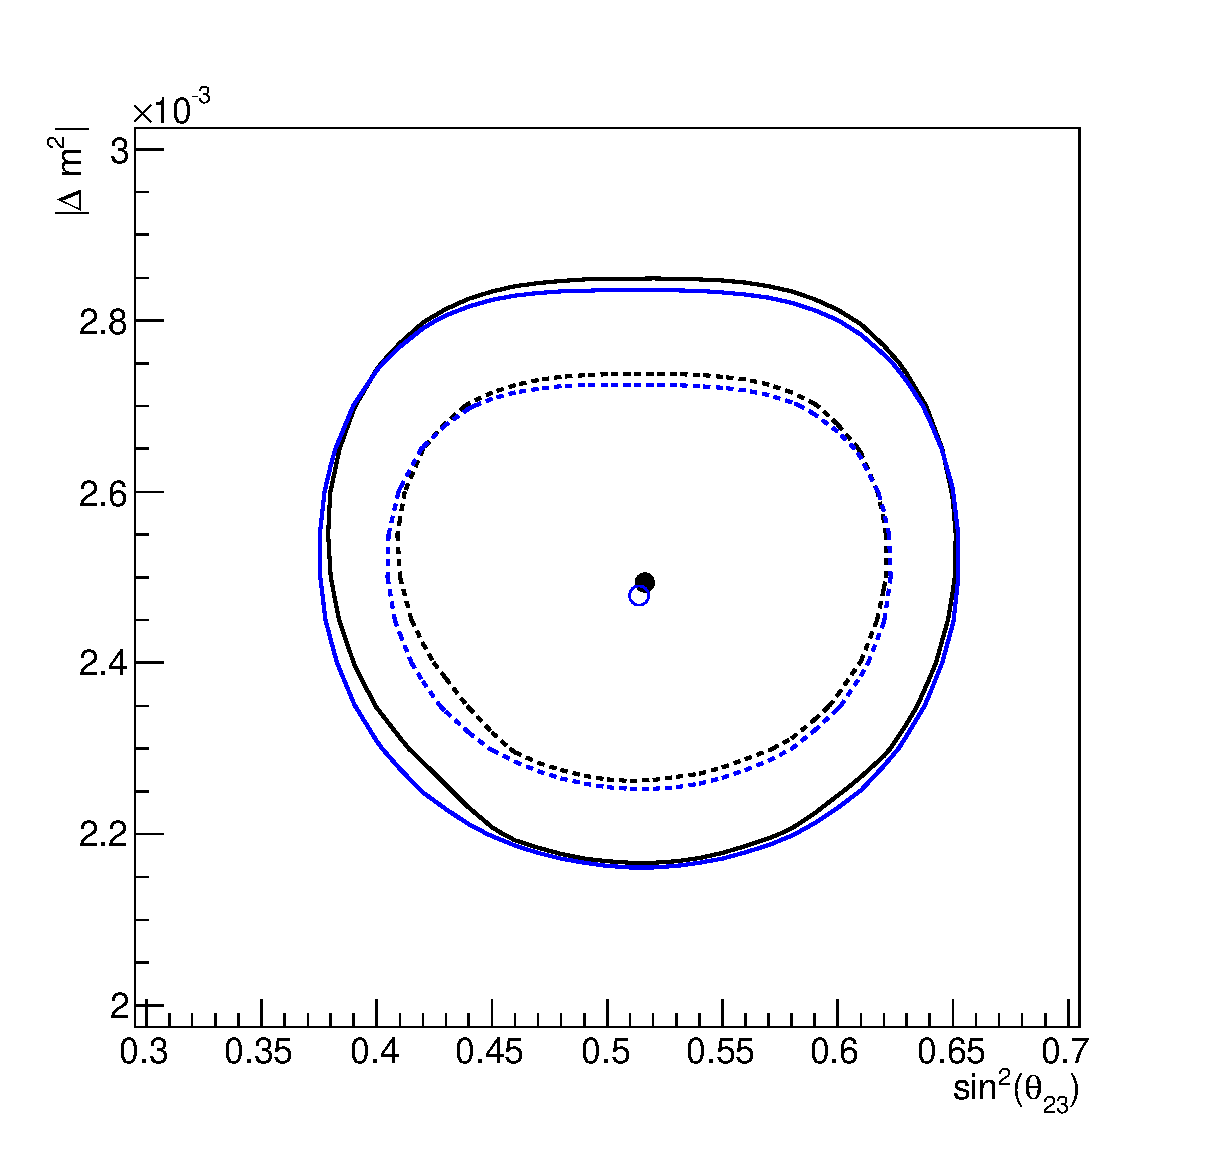
\includegraphics[width=22pc]{./images/results/data_chisq_theta23_dm23sq_global_min_new.eps}
\caption {
  68\% (dashed lines) and 90\% (solid lines) CL regions in ($sin^{2}\theta_{23}$, $|\Delta m^{2}|$) space 
  from the analysis of the Run 1+2+3 dataset
   comparing the joint analysis (black) with the stand-alone $\nu_{\mu}$ disappearance (blue)
     for Normal Hierarchy. 	
  At each point, $\chi^2$ was minimized with respect to
  all oscillation parameters not shown (and not considered to be fixed)
  and all relevant nuisance parameters.
}
\label{fig:run123_confreg_sinsqtheta23_Dmsq_nh}
\end{minipage}
\begin{minipage}[t]{0.98\linewidth}
\center
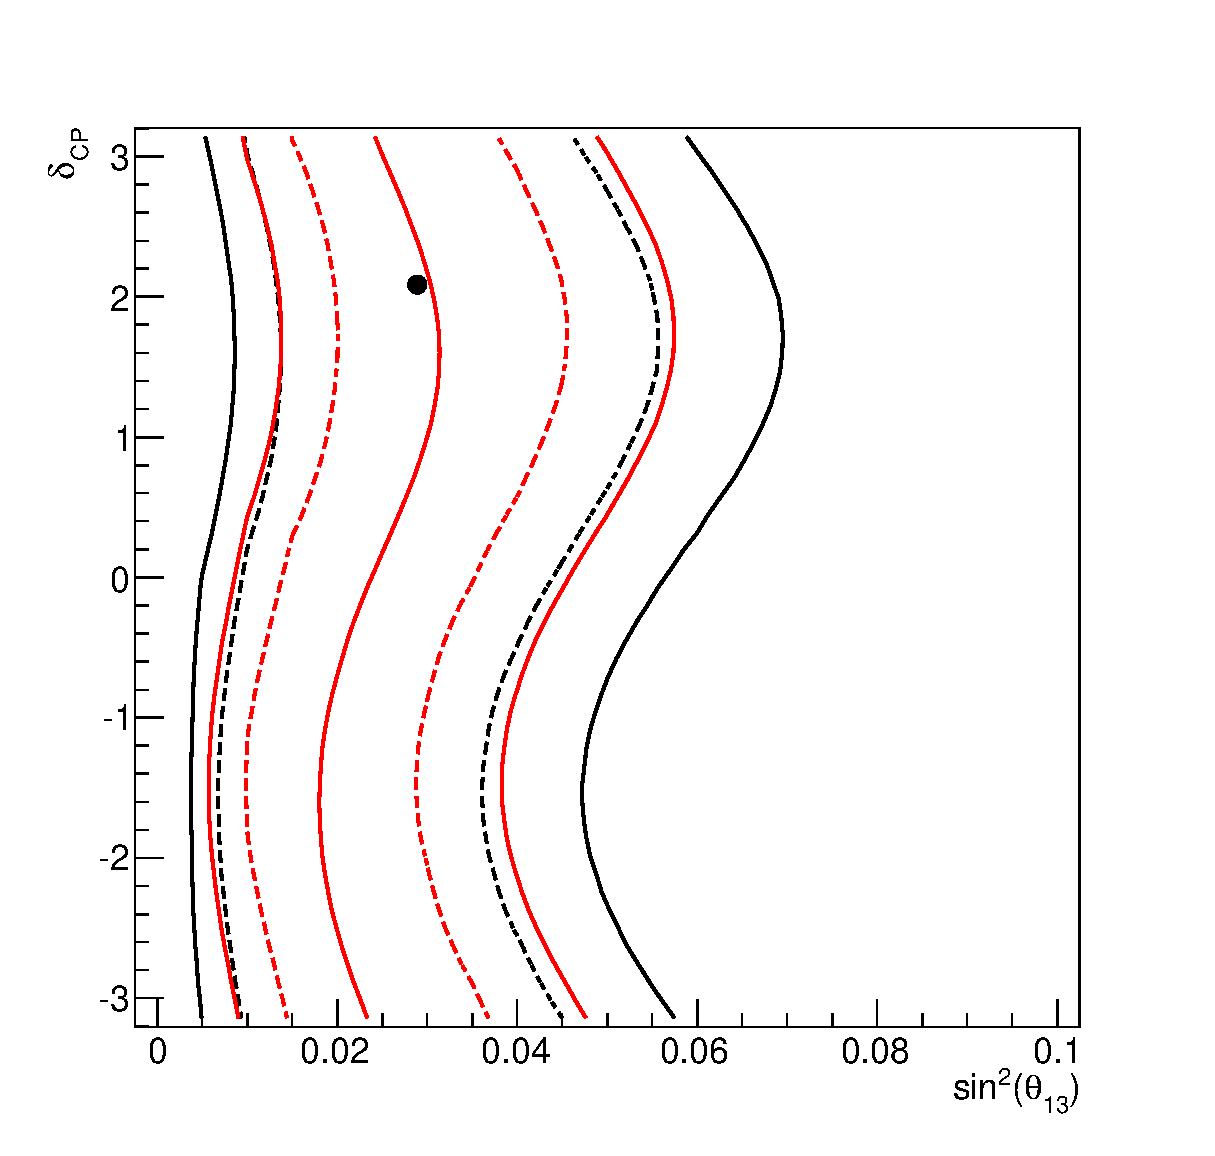
\includegraphics[width=22pc]{./images/results/data_chisq_theta13_deltacp_global_min_new.eps}
\caption {
  68\% (dashed lines) and 90\% (solid lines) CL regions in ($sin^{2}\theta_{13}$, $\delta_{CP}$) space 
  from the analysis of the Run 1+2+3 dataset
   comparing the joint analysis (black) with the stand-alone $\nu_{e}$ appearance (red)
     for Normal Hierarchy. 
  At each point, $\chi^2$ was minimized with respect to
  all oscillation parameters not shown (and not considered to be fixed)
  and all relevant nuisance parameters. Notice that different methods are used to
  construct confidence regions for the joint analysis (global minimum) and for the 
  stand-alone appearance analysis (raster scan). Middle solid red line is the line
  of best-fit points from the raster scan in the stand-alone appearance analysis.
}
\label{fig:run123_confreg_sinsqtheta13_deltacp_nh}
\end{minipage}

\end{figure*}

%...........................................................
%
% contours 
% that can not be compared with stand-alone analyses
% dmsq - sinsqtheta13, sinsqtheta23 - sinsqtheta13
%


\begin{figure*}[htb]

\begin{minipage}[t]{0.98\linewidth}
\center
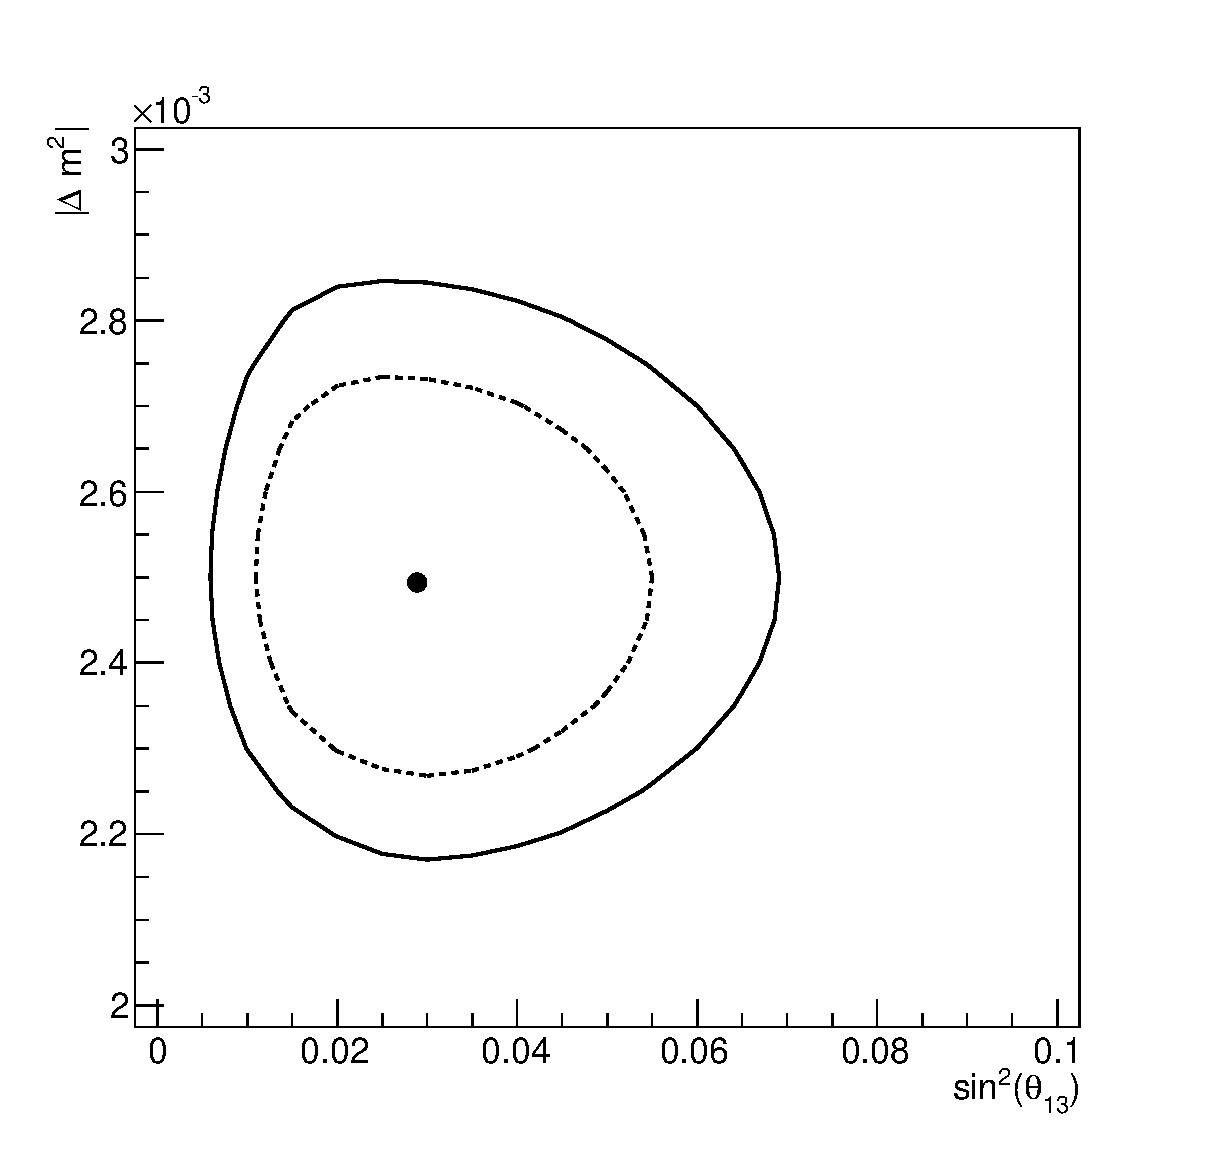
\includegraphics[width=22pc]{./images/results/data_chisq_theta13_dm23sq_global_min_new.eps}
\caption {
  68\% (dashed lines) and 90\% (solid lines) CL regions in ($sin^{2}\theta_{13}$, $|\Delta m^{2}|$) space 
  from the analysis of the Run 1+2+3 dataset  for Normal Hierarchy. 
  At each point, $\chi^2$ was minimized with respect to
  all oscillation parameters not shown (and not considered to be fixed)
  and all relevant nuisance parameters.
}
\label{fig:run123_confreg_sinsqtheta13_Dmsq_nh}
\end{minipage}
\begin{minipage}[t]{0.98\linewidth}
\center
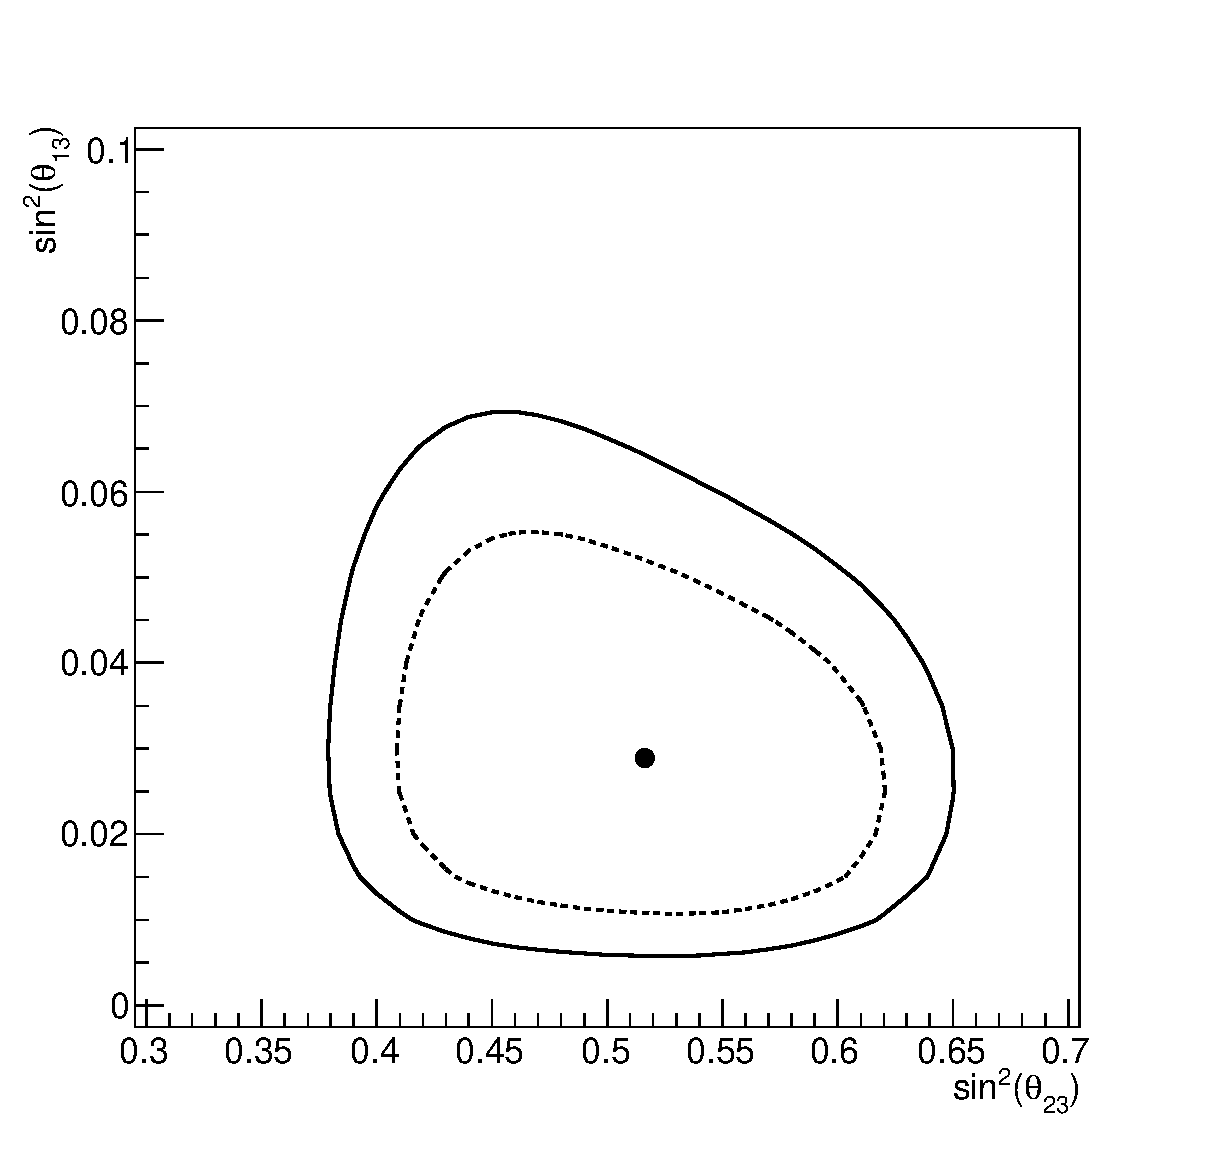
\includegraphics[width=22pc]{./images/results/data_chisq_theta13_theta23_global_min_new.eps}
\caption {
 68\% (dashed lines) and 90\% (solid lines) CL regions in ($sin^{2}\theta_{23}$, $sin^{2}\theta_{13}$) space
  from the analysis of the Run 1+2+3 dataset  for Normal Hierarchy. 
  At each point, $\chi^2$ was minimized with respect to
  all oscillation parameters not shown (and not considered to be fixed)
  and all relevant nuisance parameters.
}
\label{fig:run123_confreg_sinsqtheta23_sinsqtheta13_nh}
\end{minipage}

\end{figure*}


%...........................................................
%
% marginalized (1D) delta\chisq distributions
%

\begin{figure*}[htb]

\begin{minipage}[t]{0.45\linewidth}
\center
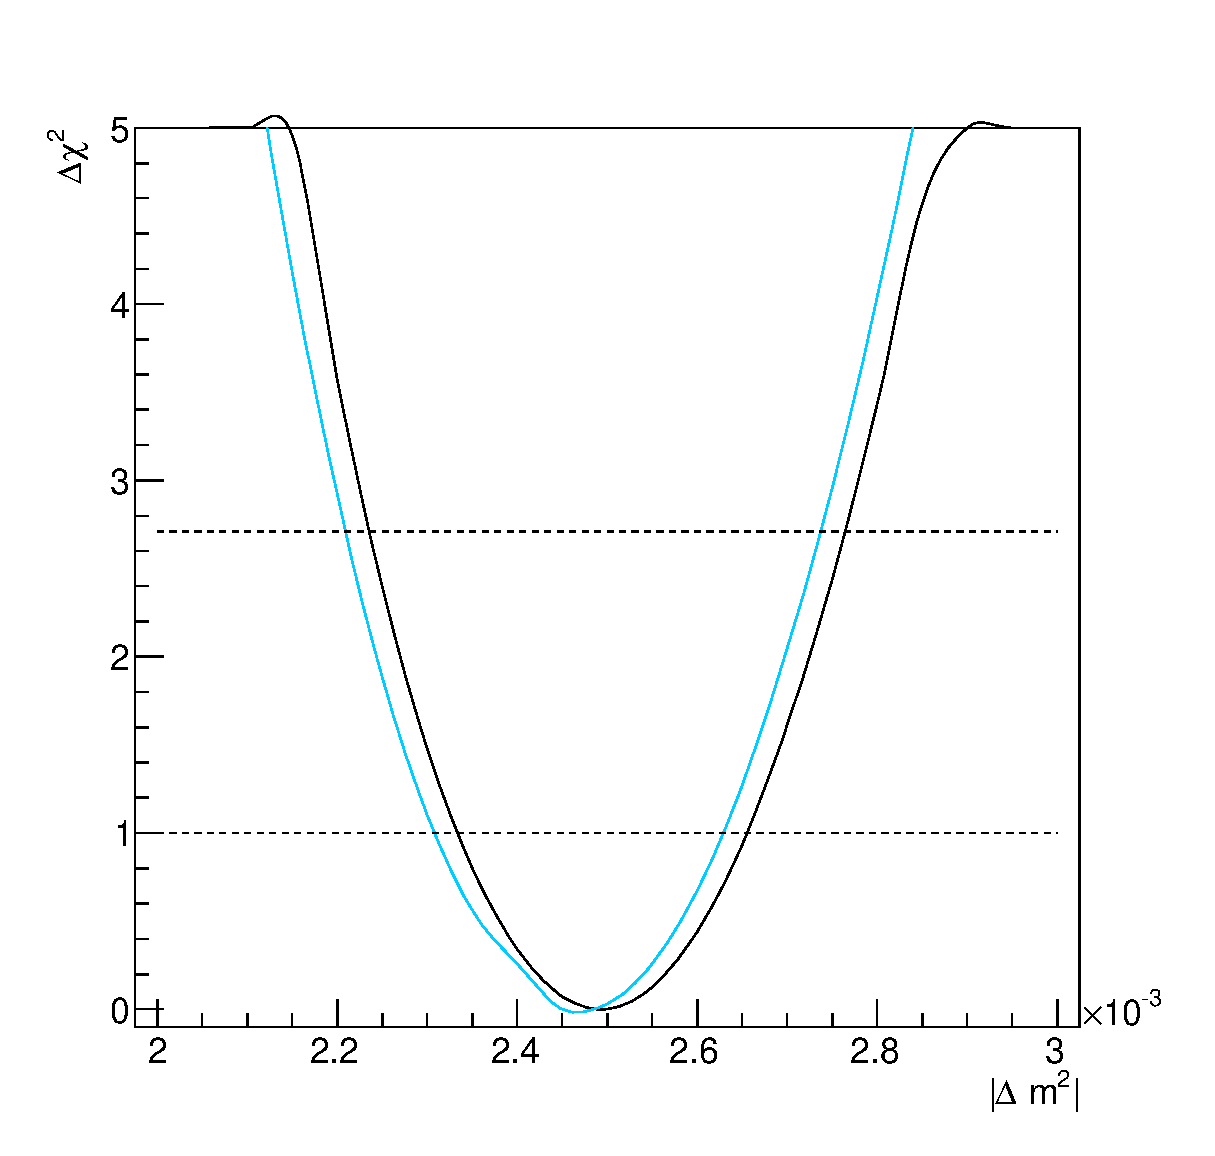
\includegraphics[width=18pc]{./images/results/data_chisq_dm23sq_global_min_mh_new.eps}
\caption {
  $\Delta\chi^2$ as function of $|\Delta m^{2}|$ from the joint 3-flavour oscillation analysis of the Run 1+2+3 dataset.
  Comparing  $\Delta\chi^2$ curves for Normal Hierarchy (black) and Inverted Hierarchy (azure).
  At each point, $\chi^2$ was minimized with respect to
  all oscillation parameters not shown (and not considered to be fixed)
  and all relevant nuisance parameters.
}
\label{fig:run123_dchisq_Dmsq_hcomp}
\end{minipage}
\hspace{0.04\linewidth}
\begin{minipage}[t]{0.45\linewidth}
\center
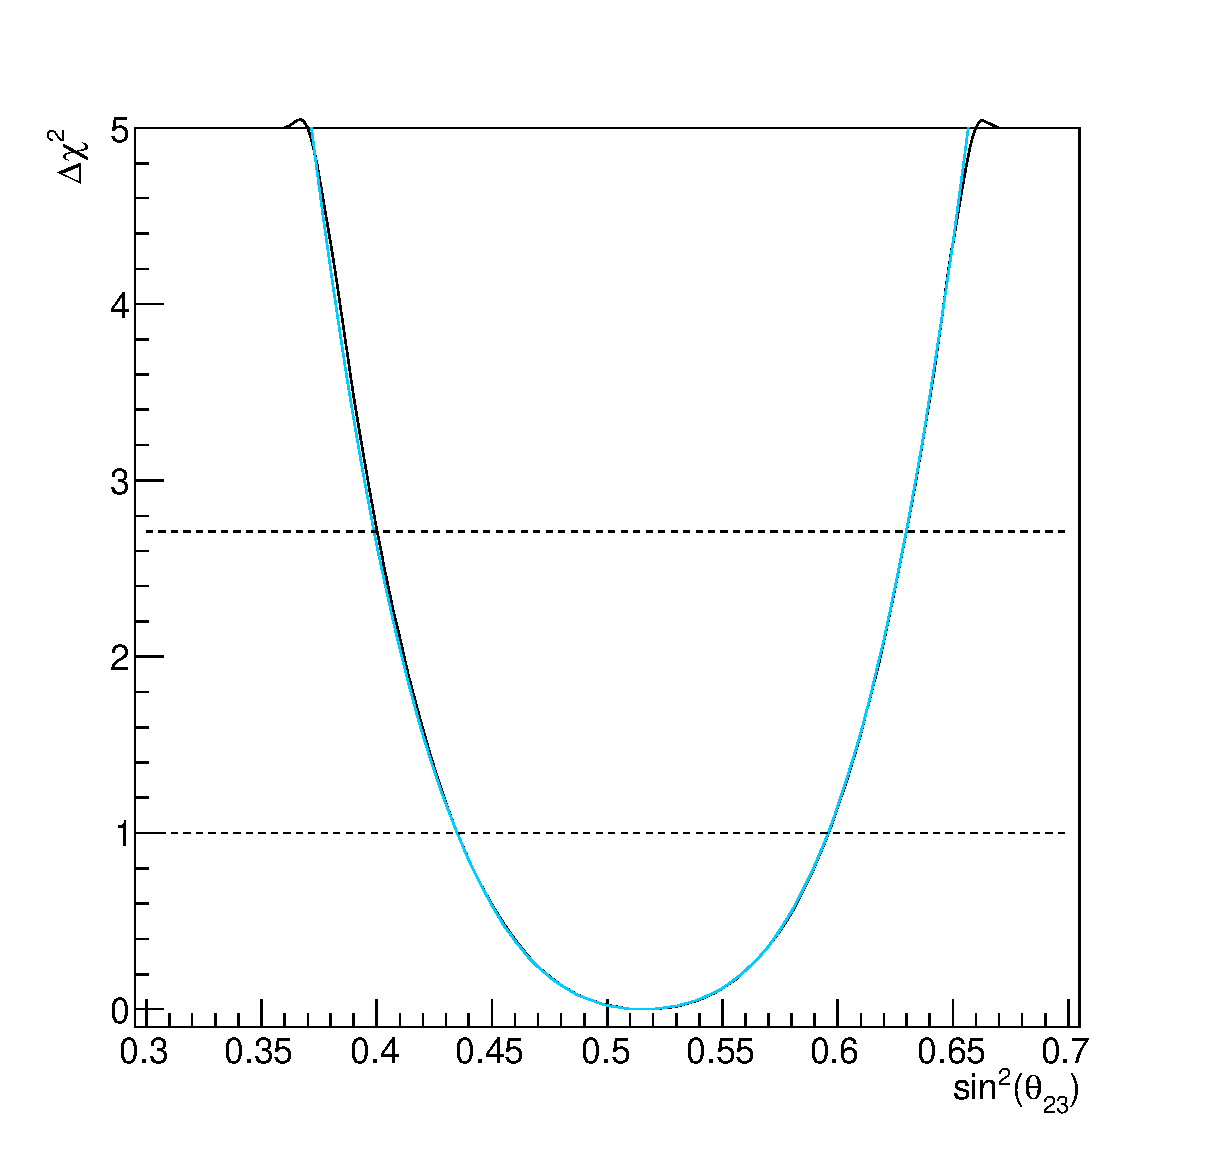
\includegraphics[width=18pc]{./images/results/data_chisq_theta23_global_min_mh_new.eps}
\caption {
  $\Delta\chi^2$ as function of $sin^{2}\theta_{23}$ from the 3-flavour oscillation analysis of the Run 1+2+3 dataset.
  Comparing $\Delta\chi^2$ curves for Normal Hierarchy (black) and Inverted Hierarchy (azure).	
  At each point, $\chi^2$ was minimized with respect to
  all oscillation parameters not shown (and not considered to be fixed)
  and all relevant nuisance parameters.
}
\label{fig:run123_dchisq_sinsqtheta23_hcomp}
\end{minipage}

\vfill
\vspace*{0.7cm}

\begin{minipage}[t]{0.45\linewidth}
\center
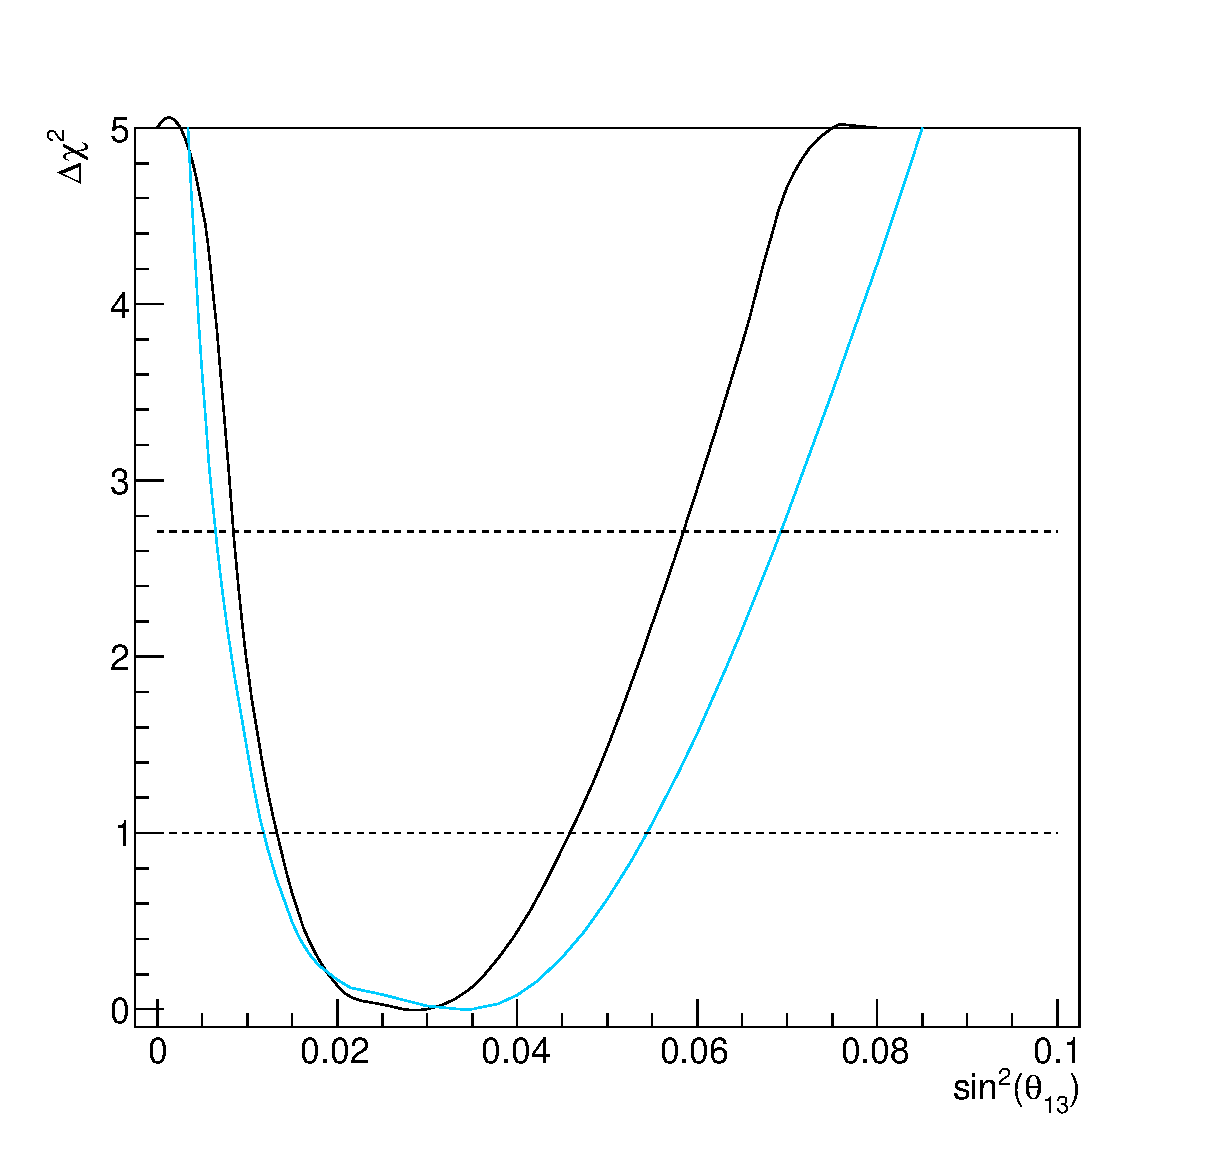
\includegraphics[width=18pc]{./images/results/data_chisq_theta13_global_min_mh_new.eps}
\caption {
  $\Delta\chi^2$ as function of $sin^{2}\theta_{13}$ from the 3-flavour oscillation analysis of the Run 1+2+3 dataset.
  Comparing $\Delta\chi^2$ curves for Normal Hierarchy (black) and Inverted Hierarchy (azure).
  At each point, $\chi^2$ was minimized with respect to
  all oscillation parameters not shown (and not considered to be fixed)
  and all relevant nuisance parameters.
}
\label{fig:run123_dchisq_sinsqtheta13_hcomp}
\end{minipage}
\hspace{0.04\linewidth}
\begin{minipage}[t]{0.45\linewidth}
\center
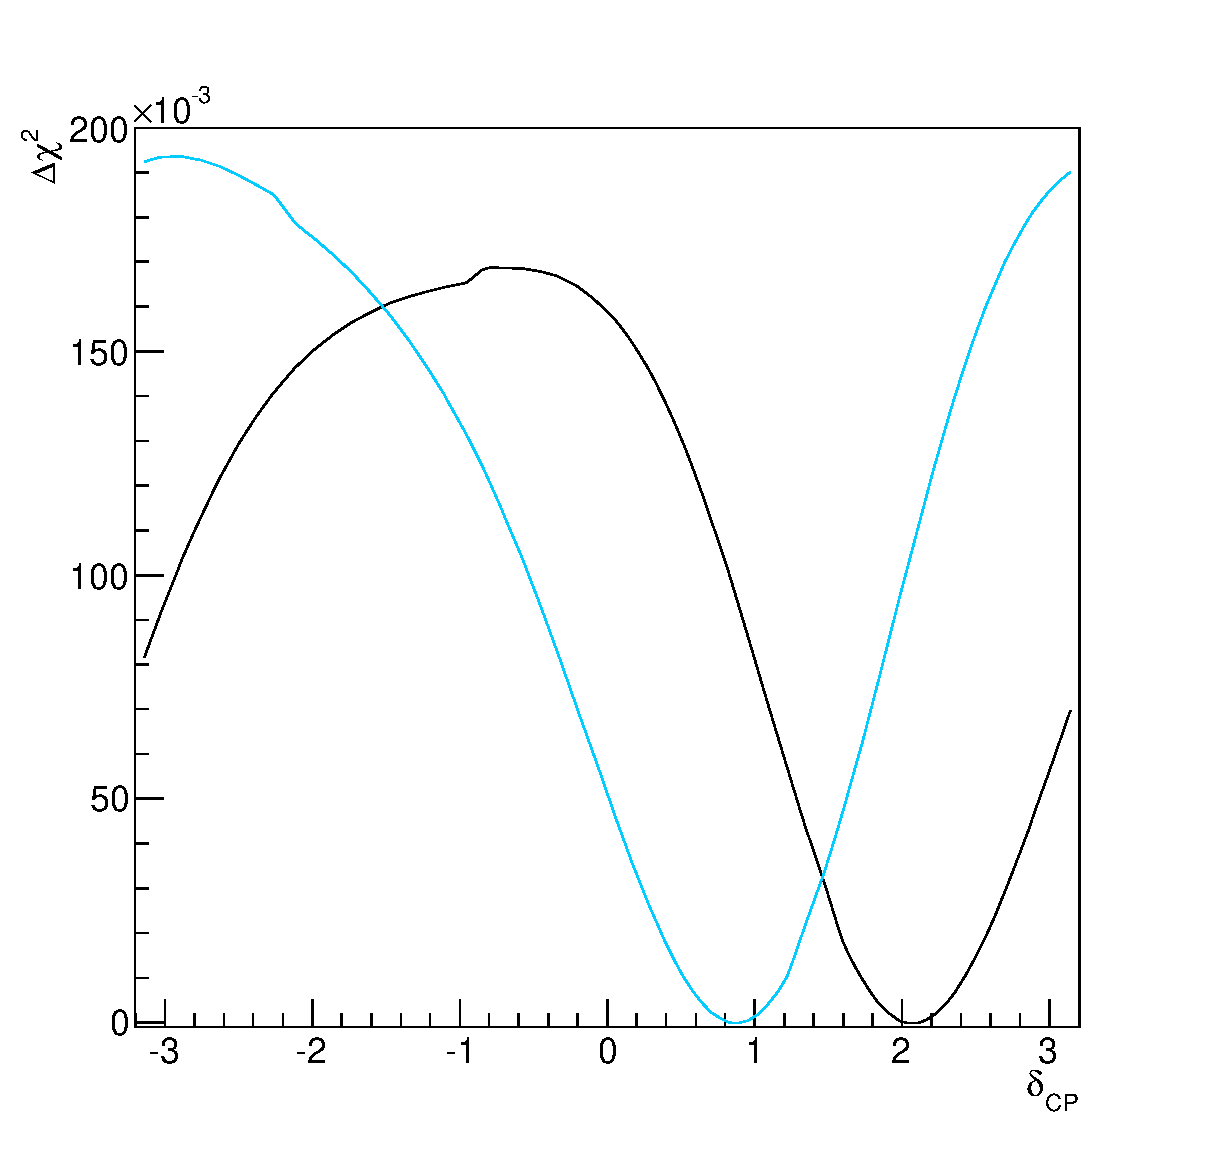
\includegraphics[width=18pc]{./images/results/data_chisq_deltacp_global_min_mh_new.eps}
\caption {
  $\Delta\chi^2$ as function of $\delta_{CP}$ from the 3-flavour oscillation analysis of the Run 1+2+3 dataset.
  Comparing $\Delta\chi^2$ curves for Normal Hierarchy (black) with Inverted Hierarchy (azure).
  At each point, $\chi^2$ was minimized with respect to
  all oscillation parameters not shown (and not considered to be fixed)
  and all relevant nuisance parameters.
}
\label{fig:run123_dchisq_deltacp_hcomp}
\end{minipage}

\end{figure*}

%...........................................................
%
% contours 
% that can be compared with stand-alone analyses
% dmsq - sinsqtheta23, deltacp - sinsqtheta13
%

\begin{figure*}[htb]

\begin{minipage}[t]{0.98\linewidth}
\center
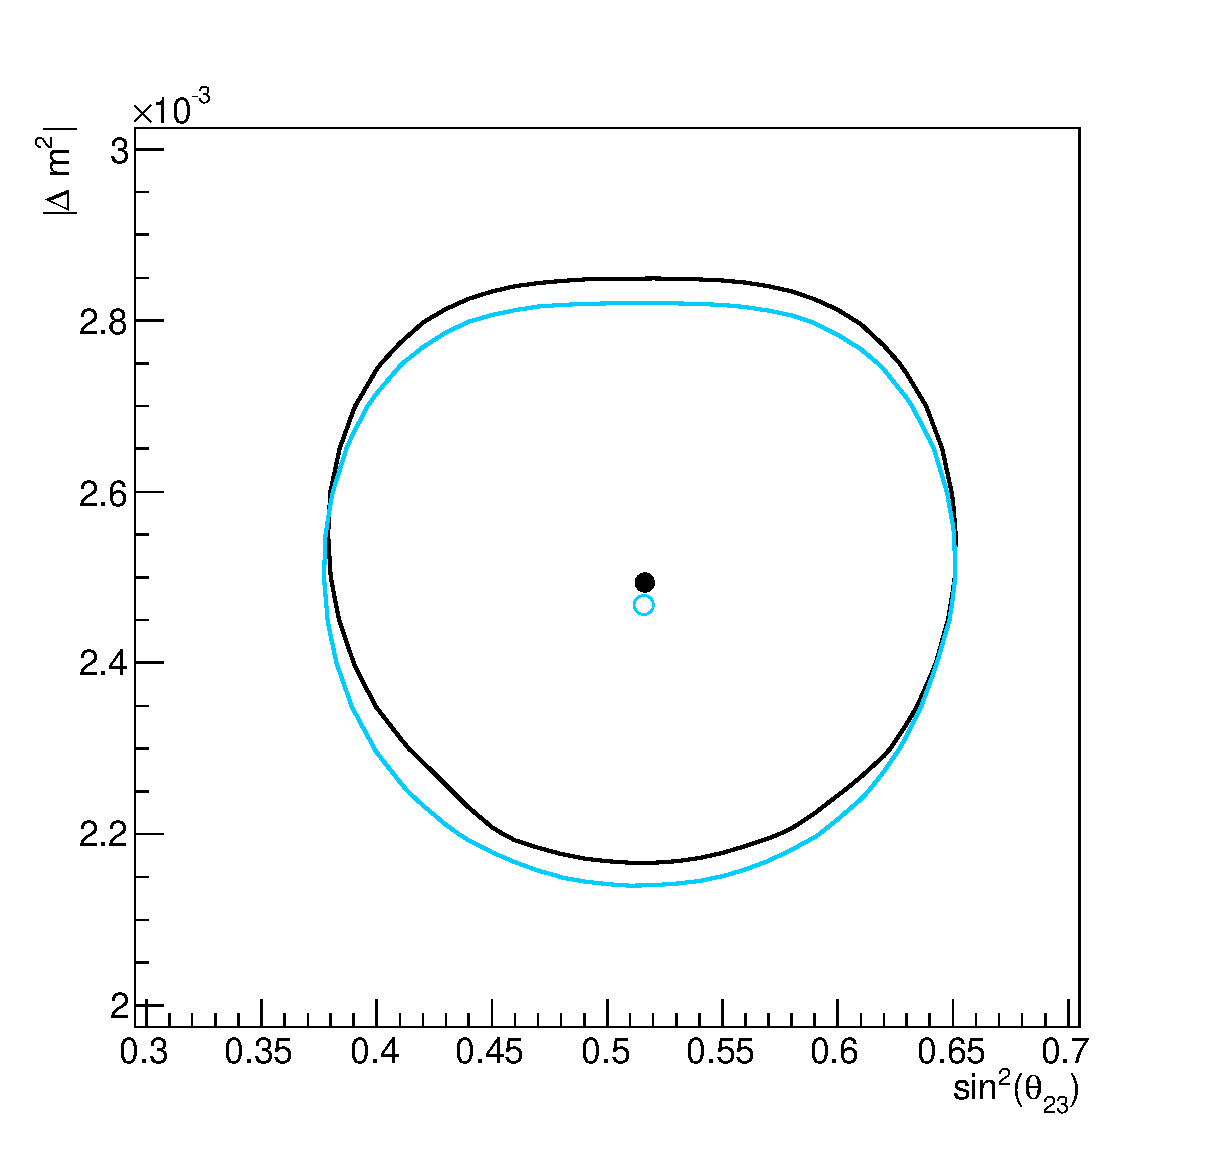
\includegraphics[width=20pc]{./images/results/data_chisq_theta23_dm23sq_global_min_mh_new.eps}
\caption {
  90\% CL regions in ($sin^{2}\theta_{23}$, $|\Delta m^{2}|$) space 
  from the joint 3-flavour oscillation analysis of the Run 1+2+3 dataset,
  comparing contours for the Normal Hierarchy (black) and Inverted Hierarchy (azure).	
  At each point, $\chi^2$ was minimized with respect to
  all oscillation parameters not shown (and not considered to be fixed)
  and all relevant nuisance parameters.
}
\label{fig:run123_confreg_sinsqtheta23_Dmsq_hcomp}
\end{minipage}
\begin{minipage}[t]{0.98\linewidth}
\center
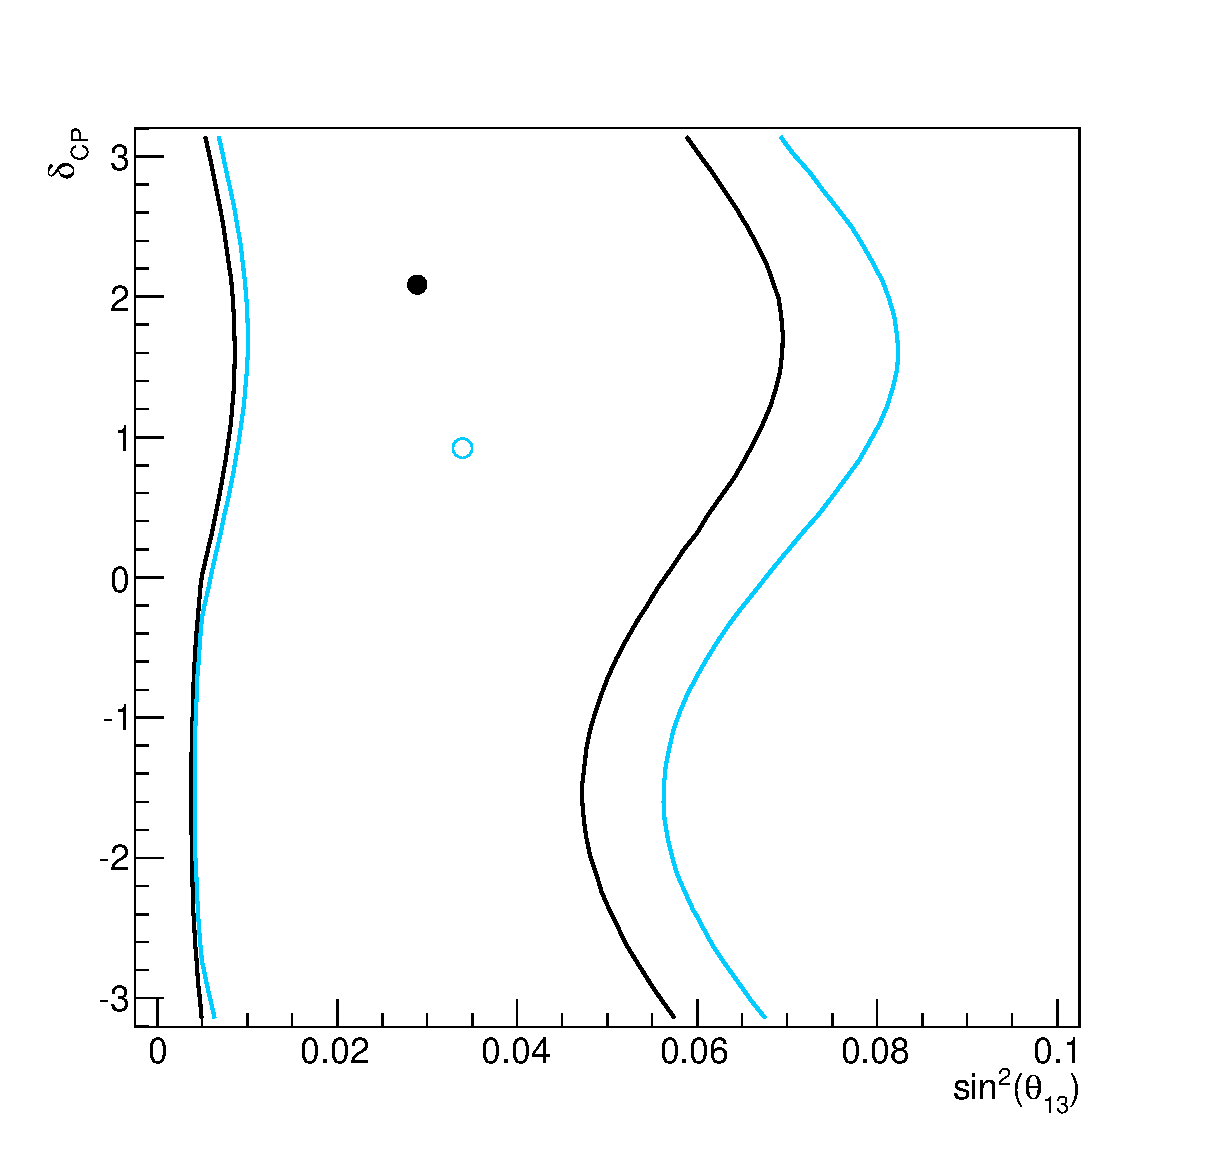
\includegraphics[width=20pc]{./images/results/data_chisq_theta13_deltacp_global_min_mh_new.eps}
\caption {
  90\% CL regions in ($sin^{2}\theta_{13}$, $\delta_{CP}$) space 
  from the joint 3-flavour oscillation analysis of the Run 1+2+3 dataset,
  comparing contours for the Normal Hierarchy (black) and Inverted Hierarchy (azure).
  At each point, $\chi^2$ was minimized with respect to
  all oscillation parameters not shown (and not considered to be fixed)
  and all relevant nuisance parameters.
}
\label{fig:run123_confreg_sinsqtheta13_deltacp_hcomp}
\end{minipage}

\end{figure*}

%...........................................................
%
% contours 
% that can not be compared with stand-alone analyses
% dmsq - sinsqtheta13, sinsqtheta23 - sinsqtheta13
%


\begin{figure*}[htb]

\begin{minipage}[t]{0.98\linewidth}
\center
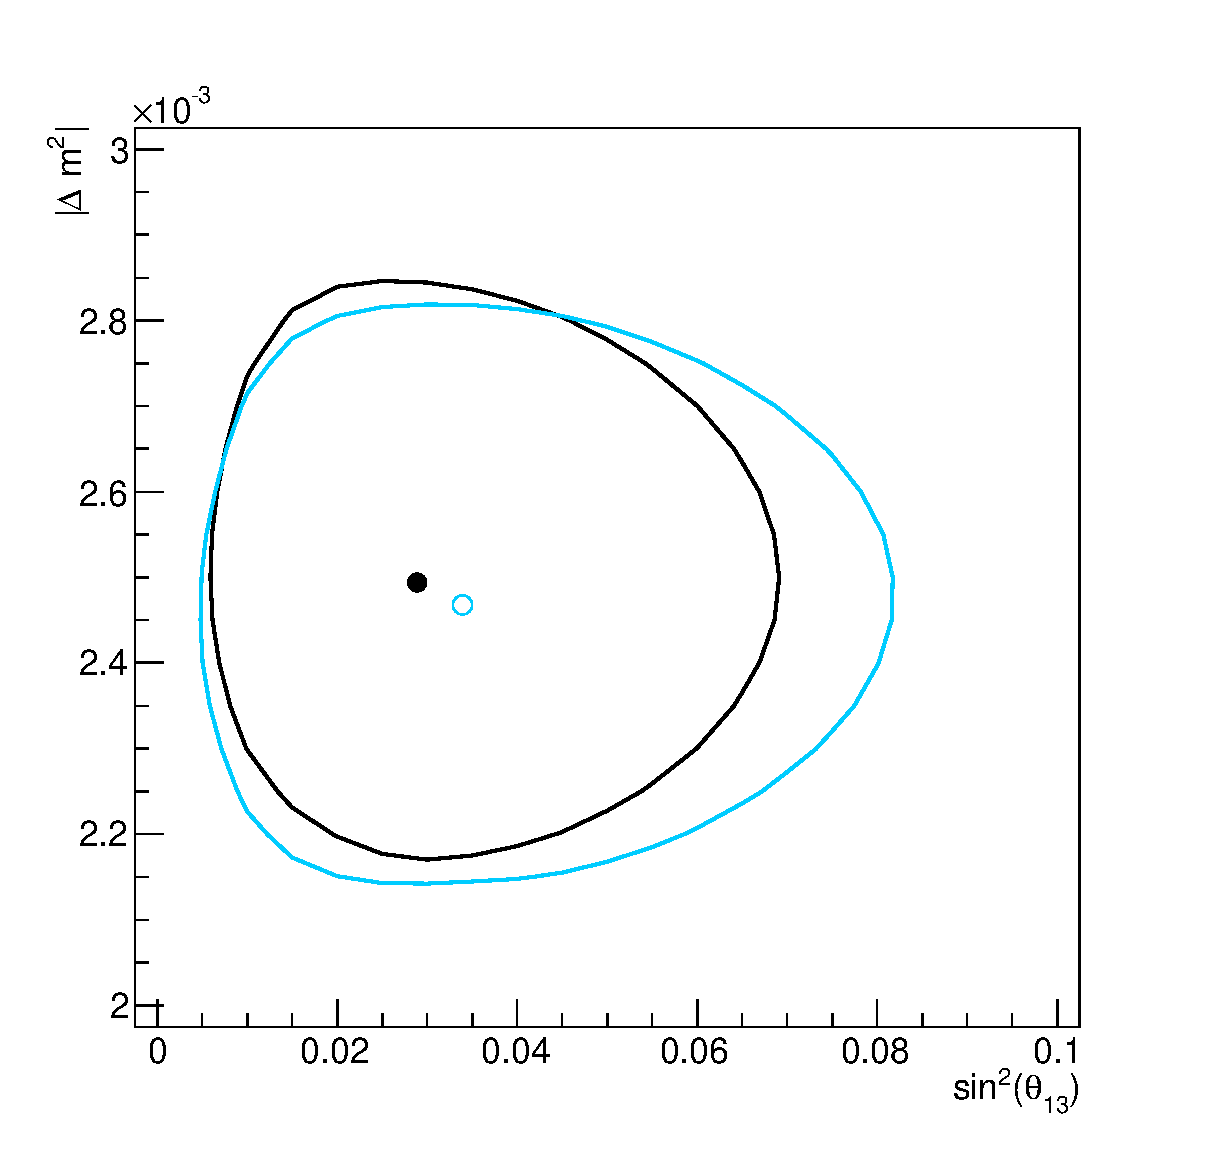
\includegraphics[width=22pc]{./images/results/data_chisq_theta13_dm23sq_global_min_mh_new.eps}
\caption {
90\% CL regions in ($sin^{2}\theta_{13}$, $|\Delta m^{2}|$) space 
  from the joint 3-flavour oscillation analysis of the Run 1+2+3 dataset,
  comparing contours for the Normal Hierarchy (black) and Inverted Hierarchy (azure).
  At each point, $\chi^2$ was minimized with respect to
  all oscillation parameters not shown (and not considered to be fixed)
  and all relevant nuisance parameters.
}
\label{fig:run123_confreg_sinsqtheta13_Dmsq_hcomp}
\end{minipage}
\begin{minipage}[t]{0.98\linewidth}
\center
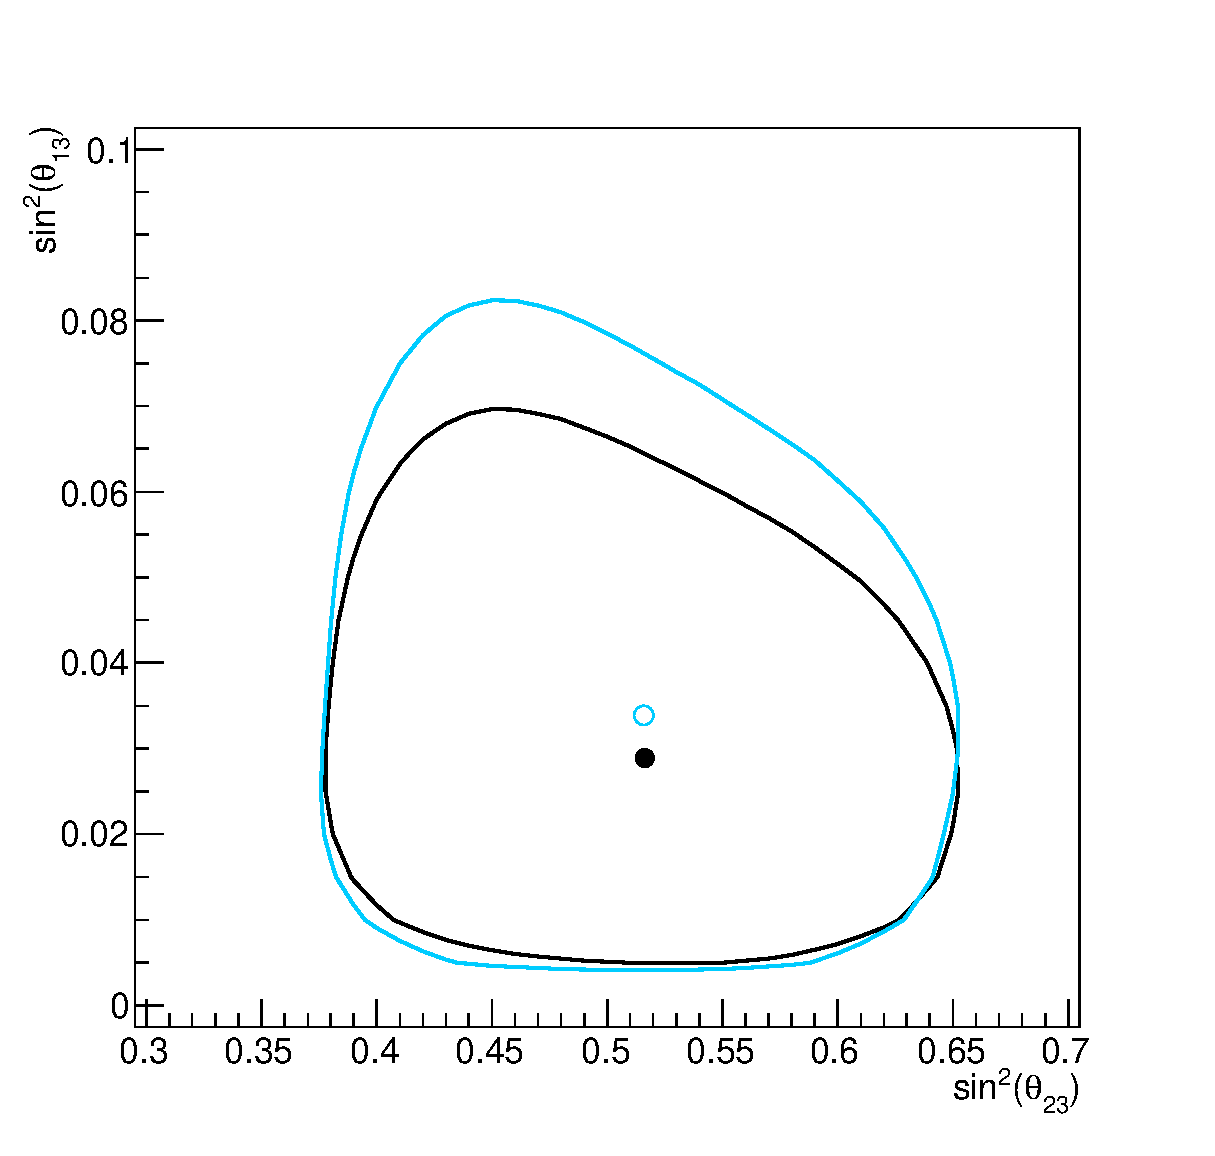
\includegraphics[width=22pc]{./images/results/data_chisq_theta13_theta23_global_min_mh_new.eps}
\caption {
  90\% CL regions in ($sin^{2}\theta_{23}$, $sin^{2}\theta_{13}$) space
  from the joint 3-flavour oscillation analysis of the Run 1+2+3 dataset,
  comparing contours for the Normal Hierarchy (black) and Inverted Hierarchy (azure).
  At each point, $\chi^2$ was minimized with respect to
  all oscillation parameters not shown (and not considered to be fixed)
  and all relevant nuisance parameters.
}
\label{fig:run123_confreg_sinsqtheta23_sinsqtheta13_hcomp}
\end{minipage}

\end{figure*}


%...........................................................
%
% m2D theta13-deltacp contours with raster scan also for joint
%

\clearpage

\begin{figure*}[htb]

\begin{minipage}[t]{0.98\linewidth}
\center
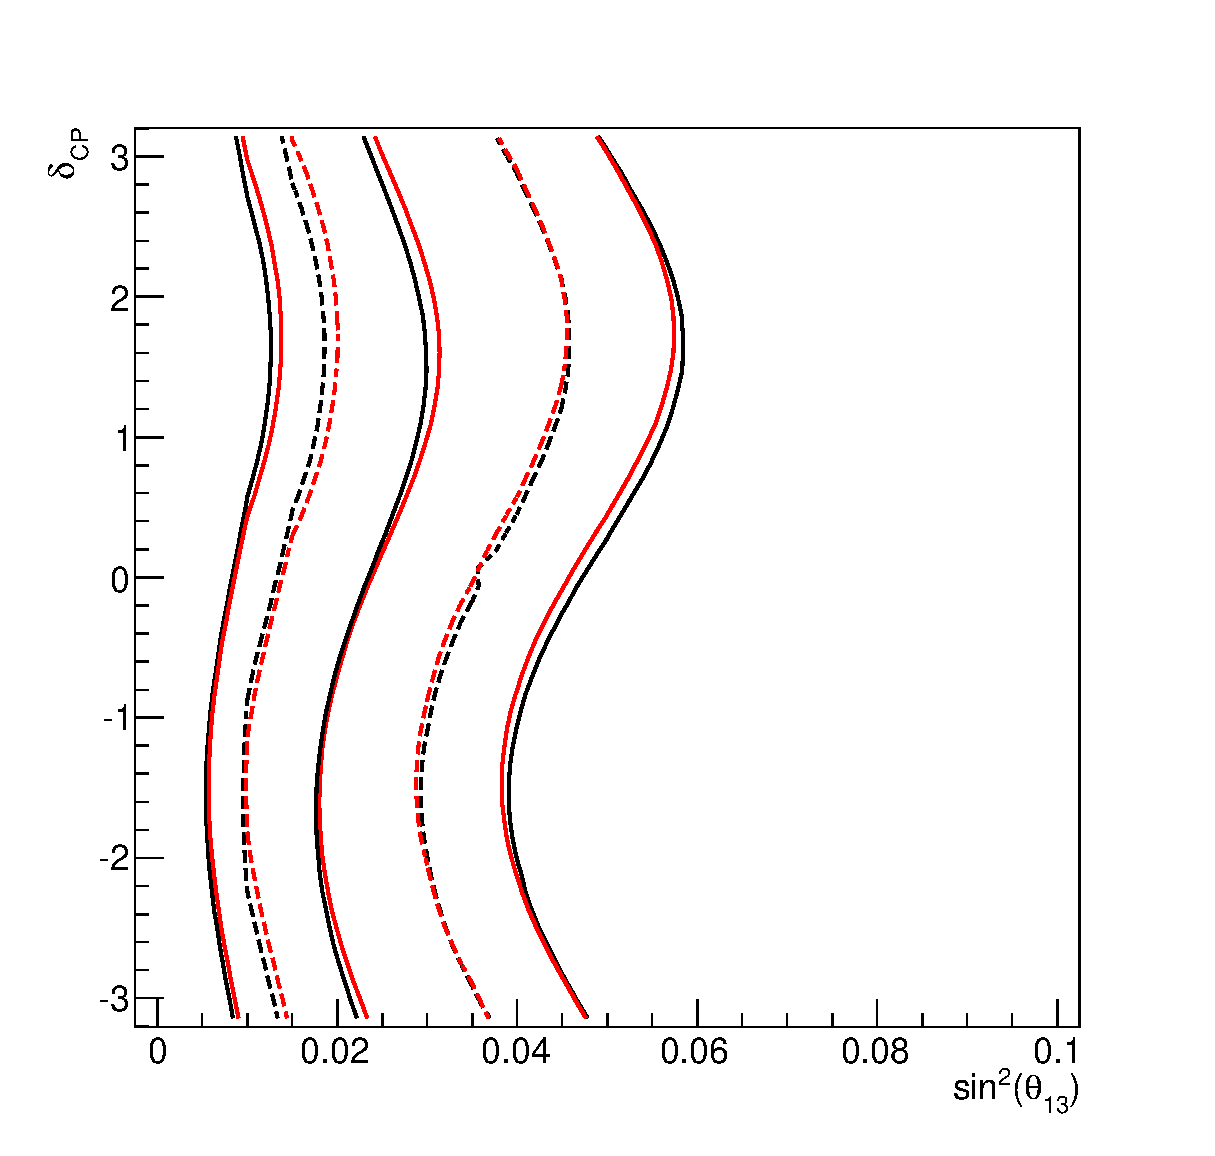
\includegraphics[width=22pc]{./images/results/data_nh_chisq_theta13_deltacp_raster.eps}
\caption {
  68\% (dashed lines) and 90\% (solid lines) CL regions in ($sin^{2}\theta_{13}$, $\delta_{CP}$) space 
  from the analysis of the Run 1+2+3 dataset
   comparing the joint analysis (black) with the stand-alone $\nu_{e}$ appearance (red)
     for Normal Hierarchy, using the raster scan in both analyses. Middle solid black (red) line is the line
  of best-fit points from the raster scan in the joint (stand-alone appearance) analysis.
 }
\label{fig:run123_confreg_sinsqtheta13_deltacp_raster_nh}
\end{minipage}
\begin{minipage}[t]{0.98\linewidth}
\center
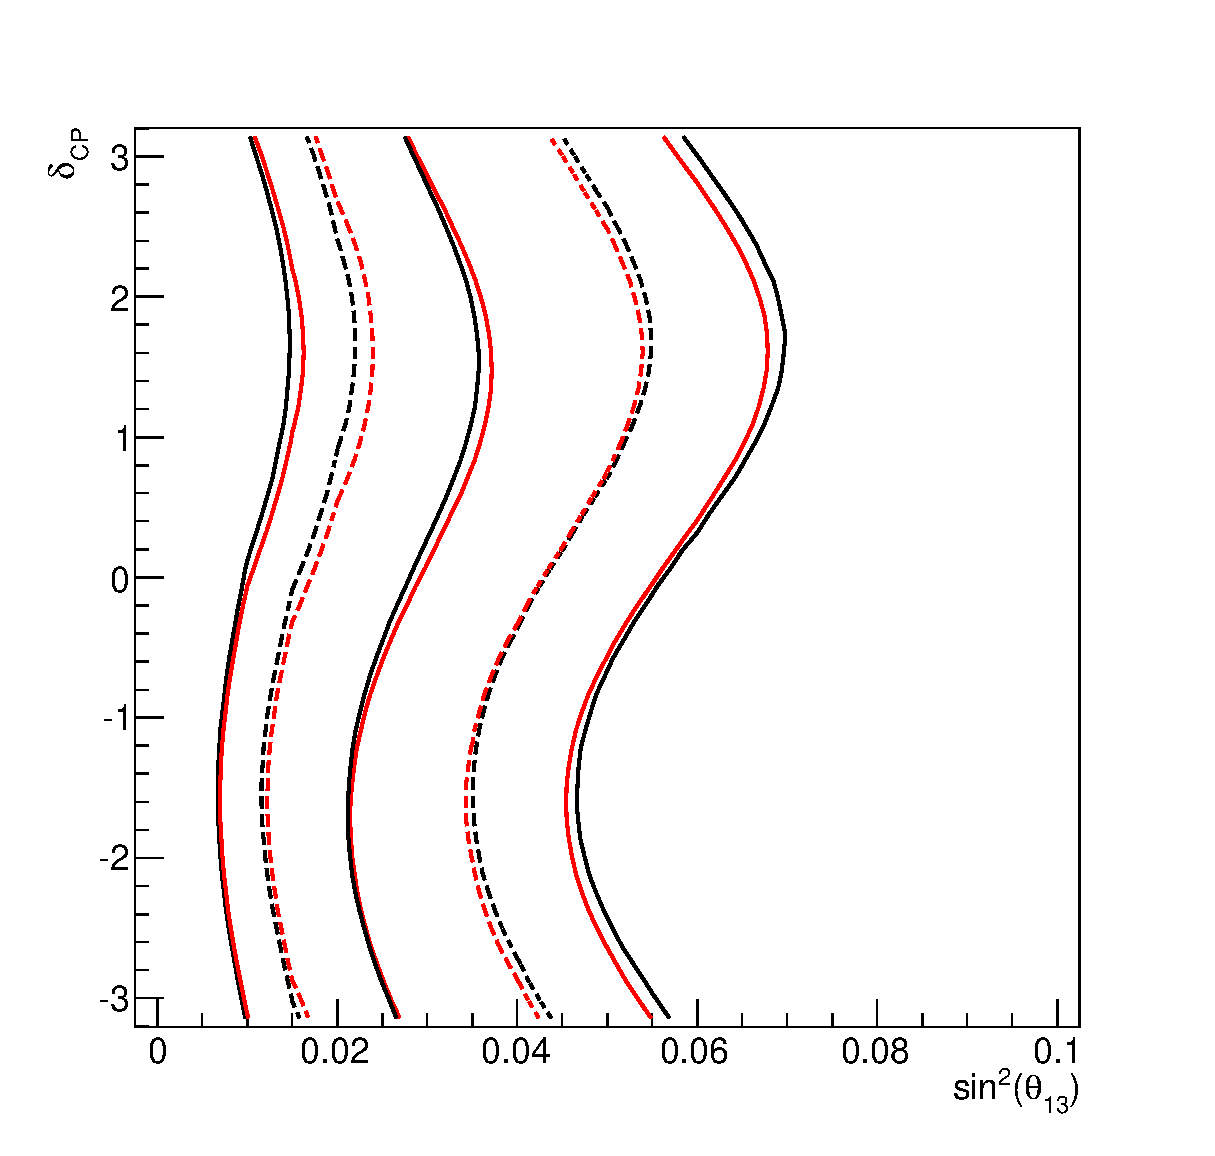
\includegraphics[width=22pc]{./images/results/data_ih_chisq_theta13_deltacp_raster.eps}
\caption {
  68\% (dashed lines) and 90\% (solid lines) CL regions in ($sin^{2}\theta_{13}$, $\delta_{CP}$) space 
  from the analysis of the Run 1+2+3 dataset
    comparing the joint analysis (black) with the stand-alone $\nu_{e}$ appearance (red)
     for Inverted Hierarchy, using the raster scan in both analyses. Middle solid black (red) line is the line
  of best-fit points from the raster scan in the joint (stand-alone appearance) analysis.
     }
\label{fig:run123_confreg_sinsqtheta13_deltacp_raster_ih}
\end{minipage}

\end{figure*}


\clearpage

%...........................................................
%
% marginalized (1D) delta\chisq distributions
%

%\begin{figure*}[htb]

%\begin{minipage}[t]{0.45\linewidth}
%\center
%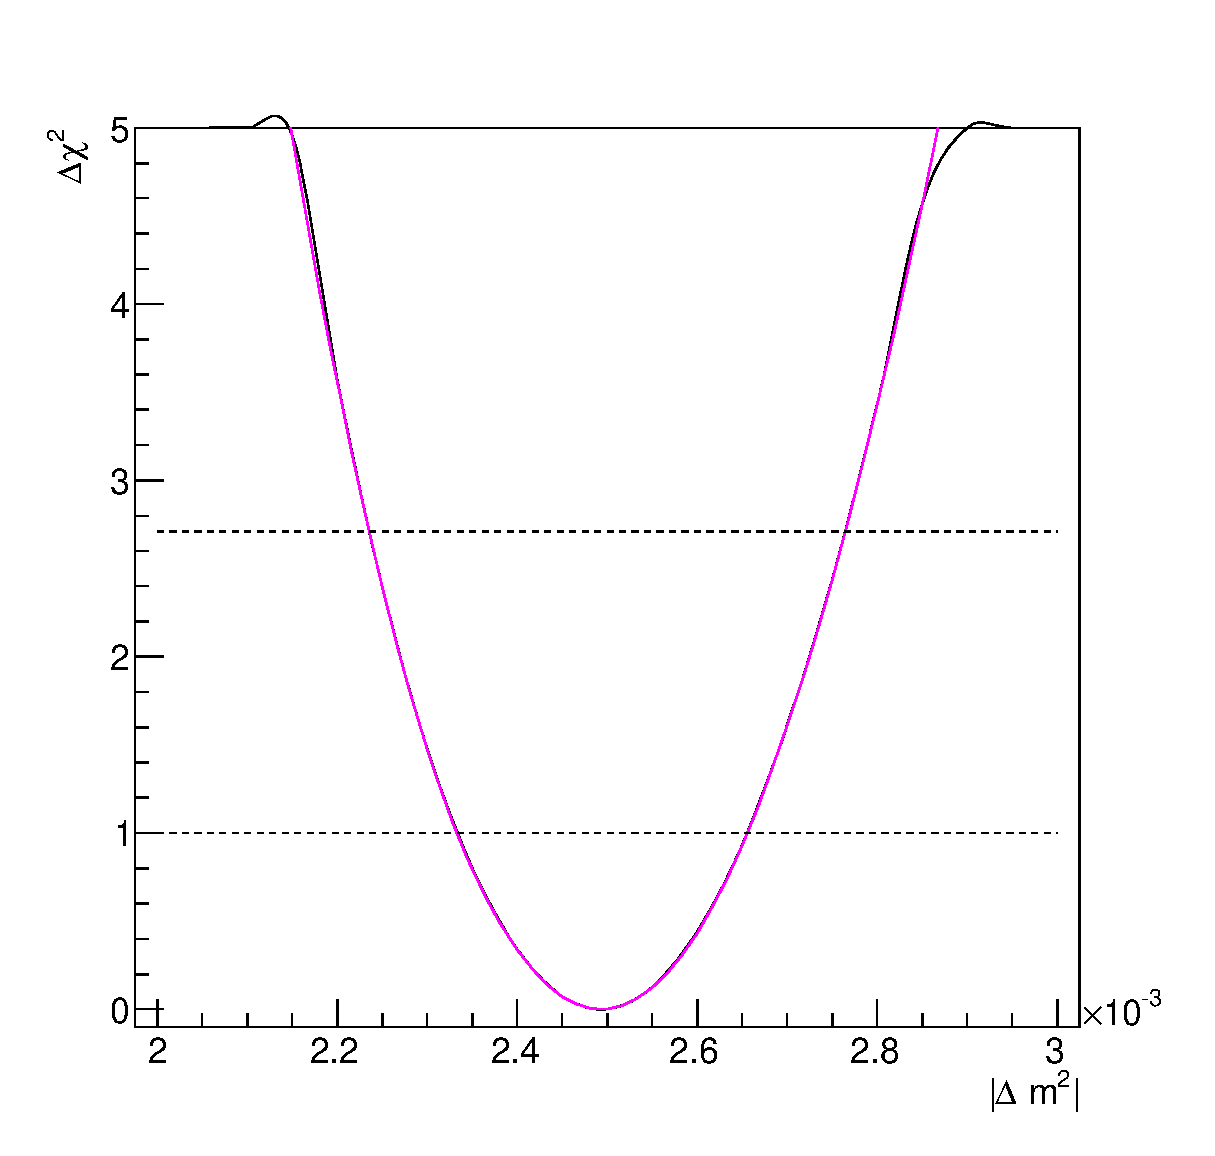
\includegraphics[width=18pc]{./images/results/data_chisq_dm23sq_global_min_2nd.eps}
%\caption {
  %$\Delta\chi^2$ as function of $|\Delta m^{2}|$ from the joint 3-flavour oscillation analysis of the Run 1+2+3 dataset.
 % Comparing $\Delta\chi^2$ curves for Normal Hierarchy with initial value in 1st octant (black) and 2nd octant (magenta).
 % At each point, $\chi^2$ was minimized with respect to
 % all oscillation parameters not shown (and not considered to be fixed)
 % and all relevant nuisance parameters.
%}
%\label{fig:run123_dchisq_Dmsq_octcomp}
%\end{minipage}

%\vfill
%\vspace*{0.7cm}

%\begin{minipage}[t]{0.45\linewidth}
%\center
%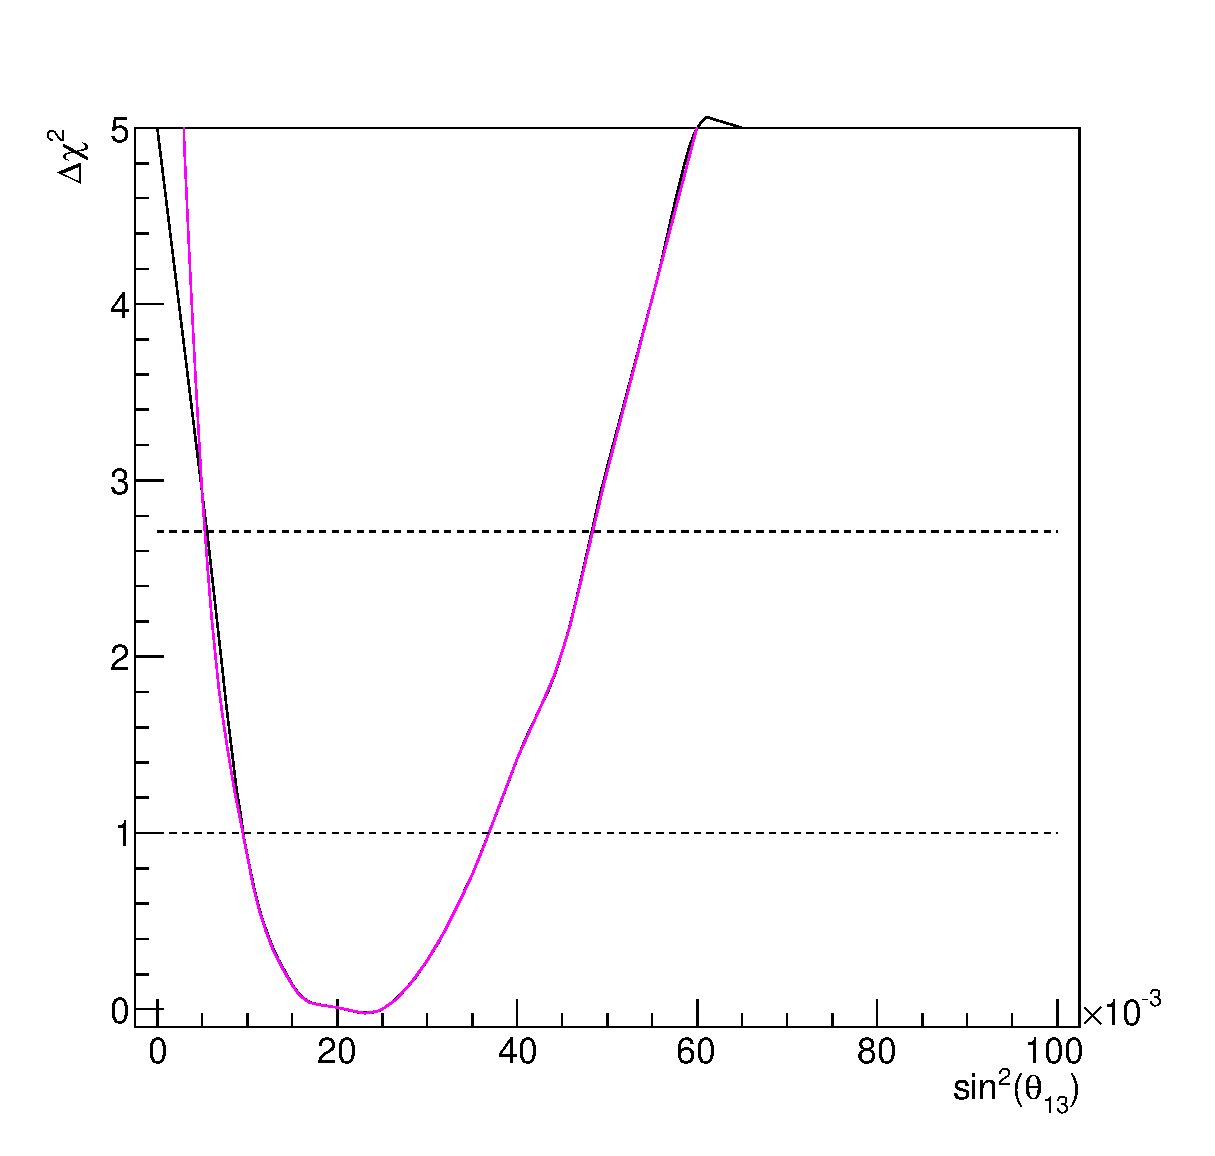
\includegraphics[width=18pc]{./images/results/data_chisq_theta13_global_min_2nd.eps}
%\caption {
 % $\Delta\chi^2$ as function of $sin^{2}\theta_{13}$ from the joint 3-flavour oscillation analysis of the Run 1+2+3 dataset.
 % Comparing $\Delta\chi^2$ curves for Normal Hierarchy with initial value in 1st octant (black) and 2nd octant (magenta).
 % At each point, $\chi^2$ was minimized with respect to
 % all oscillation parameters not shown (and not considered to be fixed)
 % and all relevant nuisance parameters.
%}
%\label{fig:run123_dchisq_sinsqtheta13_octcomp}
%\end{minipage}
%\hspace{0.04\linewidth}
%\begin{minipage}[t]{0.45\linewidth}
%\center
%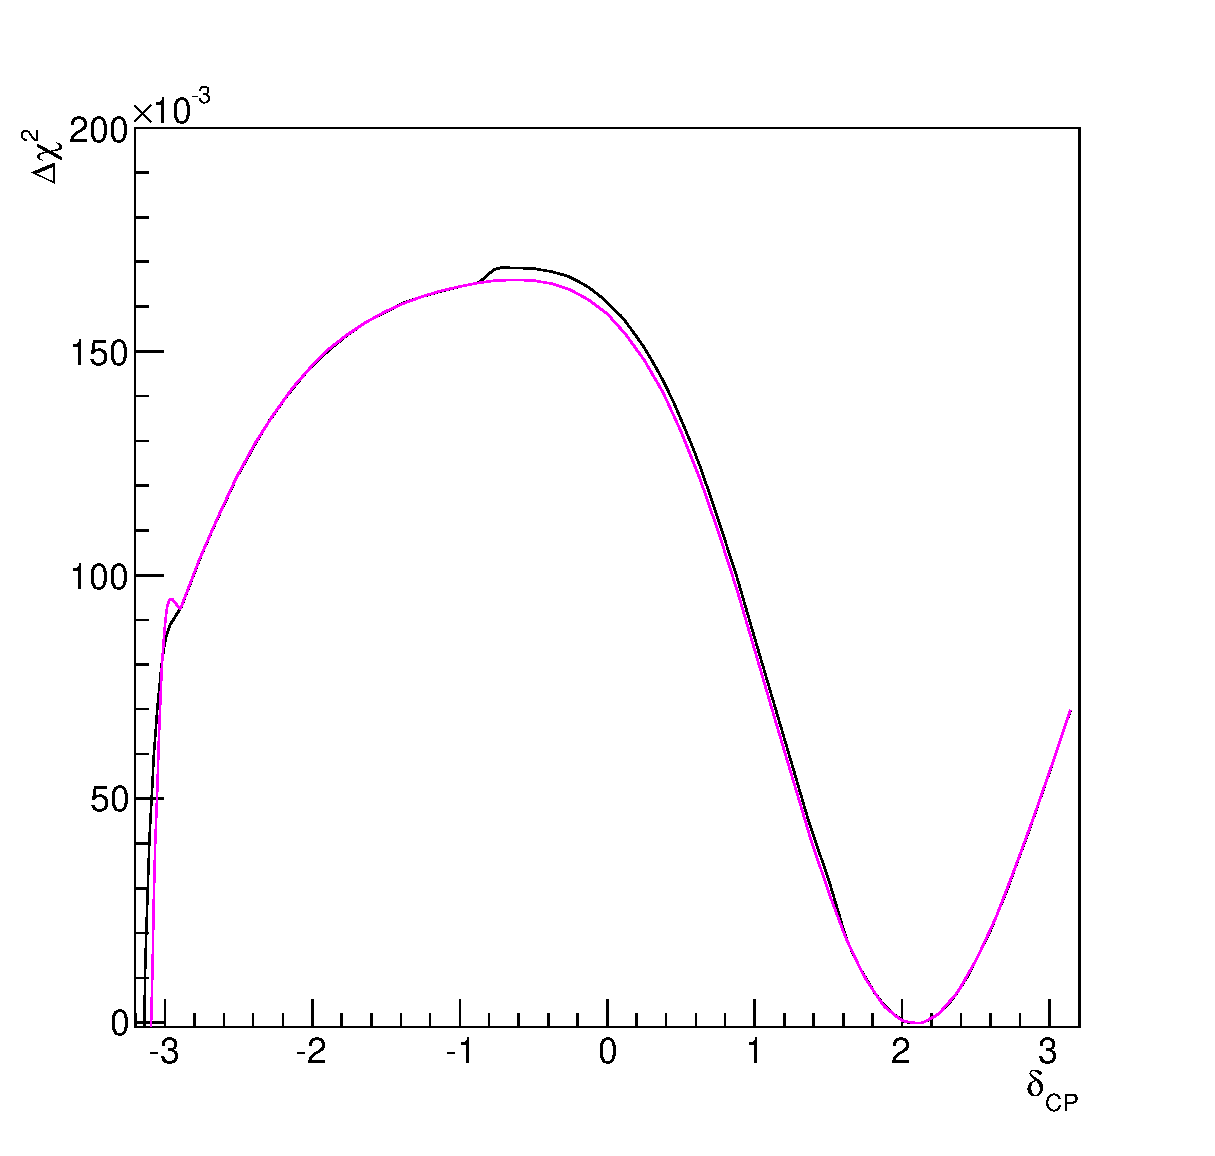
\includegraphics[width=18pc]{./images/results/data_chisq_deltacp_global_min_2nd.eps}
%\caption {
  %$\Delta\chi^2$ as function of $\delta_{CP}$ from the joint 3-flavour oscillation analysis of the Run 1+2+3 dataset.
  %Comparing $\Delta\chi^2$ curves for Normal Hierarchy with initial value in 1st octant (black) and 2nd octant (magenta).
  %At each point, $\chi^2$ was minimized with respect to
  %all oscillation parameters not shown (and not considered to be fixed)
  %and all relevant nuisance parameters.
%}
%\label{fig:run123_dchisq_deltacp_octcomp}
%\end{minipage}

%\end{figure*}


%...........................................................
%
% contours 
% that can not be compared with stand-alone analyses
% dmsq - sinsqtheta13, sinsqtheta23 - sinsqtheta13
%


%\begin{figure*}[htb]
%\begin{minipage}[t]{0.98\linewidth}
%\center
%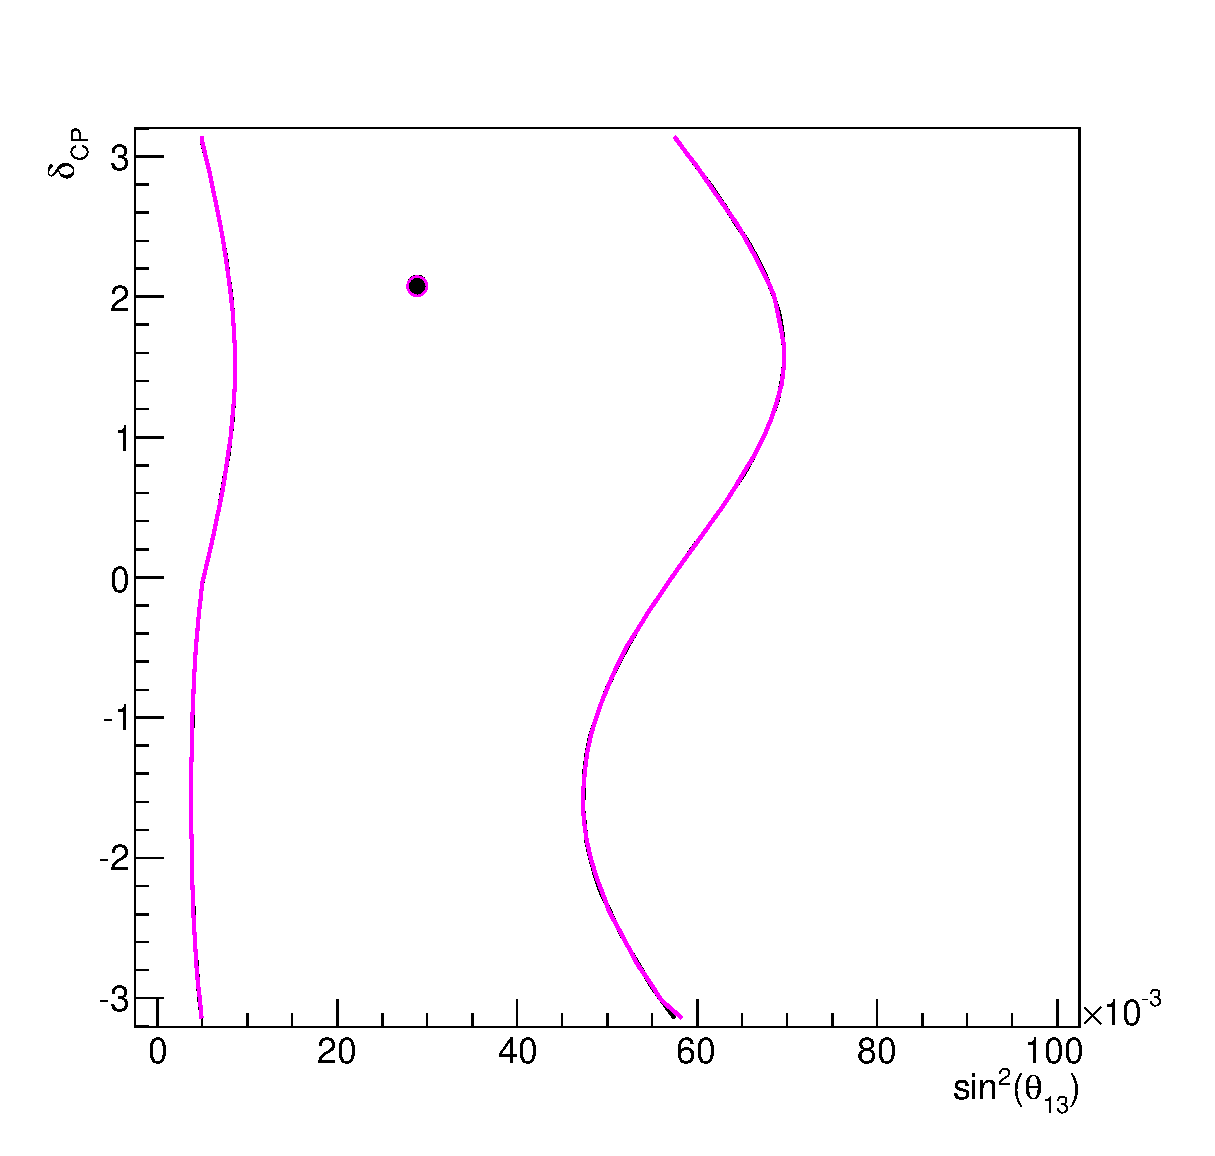
\includegraphics[width=22pc]{./images/results/data_chisq_theta13_deltacp_global_min_2nd.eps}
%\caption {
 % 68\% and 90\% CL regions in ($sin^{2}\theta_{13}$, $\delta_{CP}$) space 
  %from the joint 3-flavour oscillation analysis of the Run 1+2+3 dataset.
 % Comparing contours for Normal Hierarchy with initial value in 1st octant (black) and 2nd octant (magenta).
 % At each point, $\chi^2$ was minimized with respect to
 % all oscillation parameters not shown (and not considered to be fixed)
 % and all relevant nuisance parameters.
%}
%\label{fig:run123_confreg_sinsqtheta13_deltacp_octcomp}
%\end{minipage}
%\begin{minipage}[t]{0.98\linewidth}
%\center
%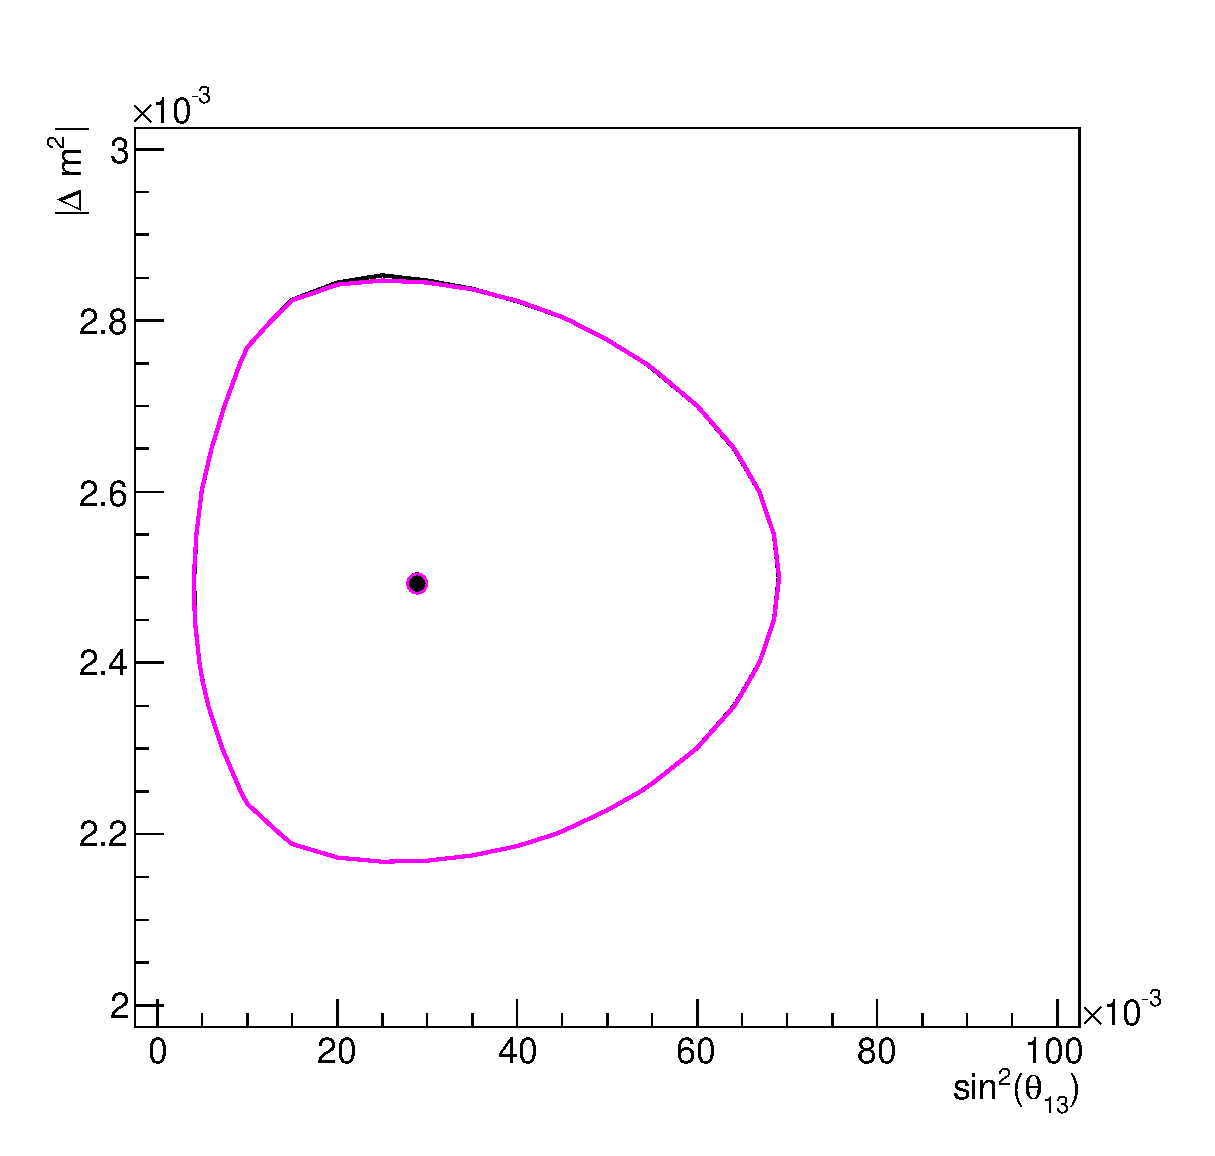
\includegraphics[width=22pc]{./images/results/data_chisq_theta13_dm23sq_global_min_2nd.eps}
%\caption {
 % 68\% and 90\% CL regions in ($sin^{2}\theta_{13}$, $|\Delta m^{2}|$) space 
  %from the joint 3-flavour oscillation analysis of the Run 1+2+3 dataset.
 % Comparing contours for Normal Hierarchy with initial value in 1st octant (black) and 2nd octant (magenta).
 % At each point, $\chi^2$ was minimized with respect to
 % all oscillation parameters not shown (and not considered to be fixed)
 % and all relevant nuisance parameters.
%}
%\label{fig:run123_confreg_sinsqtheta13_Dmsq_octcomp}
%\end{minipage}
%\end{figure*}







% Summary
\clearpage 

\section {Summary}
\label{sec:summary}

This technical note reports a joint 3-flavour oscillation analysis by the VaLOR group on the combined Run 1+2+3 dataset, 
which corresponds to an integrated neutrino beam exposure of 3.020$\times$10$^{20}$ POT. 
The joint analysis determines $|\Delta m^{2}|$, $\sin^{2} \theta_{23}$,  $\sin^{2} \theta_{13}$ and $\delta_{CP}$ together 
by making a simultaneous fit of the reconstructed energy spectra of the single $\mu$-like ring and single e-like ring SuperK event samples. 
This fit is performed in a 3-flavour framework including constant-density matter effects. Official 2012 T2K analysis inputs are used, 
and all 83 systematic parameters considered in the analysis (see Sec.\ \ref{sec:systematics}) are allowed to float in the fit. 
The Fogli-Lisi convention is used for the ``atmospheric'' mass-squared splitting $|\Delta m^{2}|$ (see Sec.\ \ref{sec:oscparamchoice}). 
The ``solar'' oscillation parameters $\sin^{2} \theta_{12}$ and $\Delta m_{21}^{2}$ have been found to have a negligible effect (see appendix \ref{app:solar}), 
and are fixed at 0.311 and 7.5$\times$10$^{-5}$ eV$^{2}$/c$^{4}$ respectively (the 2012 PDG values). 

This analysis has been extensively validated. The $\nu_{\mu}$-disappearance analysis is identical to the 2012 VaLOR analysis reported in Ref.\ \cite{OurRun123DisappAnalysis3Flavour}, 
and the $\nu_{e}$-appearance analysis has been validated against the official 2012 analyses (see appendix \ref{app:standalone}). 
Studies have been made of fitter residuals (appendix \ref{app:fitter_performance}), fits of 3.020$\times$10$^{20}$ POT fake datasets (appendix \ref{app:fake_dataset_fits}) 
and the T2K expected sensitivity for 3.020$\times$10$^{20}$ POT (appendix \ref{app:sensitivity}). These studies have shown that the joint analysis fitter is performing as expected. 

In the present version of the analysis, correlations between the single $\mu$-like ring and single e-like ring systematic uncertainties have been neglected, 
but they will be studied and reported in a future version. 

For the normal hierarchy (NH), the joint analysis fit of the reconstructed energy spectra of the single $\mu$-like ring and single e-like ring SuperK event samples gives
$|\Delta m^{2}|$ = 2.494$\times$10$^{-3}$ $eV^{2}/c^{4}$,
$\sin^{2}\theta_{23}$ = 0.516,
$\sin^{2}\theta_{13}$ = 0.029 and
$\delta_{CP}$ = 2.086.
The corresponding best-fit values for the inverted hierarchy (IH) are 
$|\Delta m^{2}|$ = 2.468$\times$10$^{-3}$ $eV^{2}/c^{4}$,
$\sin^{2}\theta_{23}$ = 0.516,
$\sin^{2}\theta_{13}$ = 0.034 and
$\delta_{CP}$ = 0.922.

Confidence regions are constructed using the constant-$\Delta\chi^2$ method.
For the NH, the 90\% (68\%) C.L. allowed region for the four fitted oscillation parameters can be summarized as
2.227$\times$10$^{-3}$ (2.332$\times$10$^{-3}$) eV$^{2}$/c$^{4}$
$< |\Delta m^{2}| < $
2.773$\times$10$^{-3}$ (2.659$\times$10$^{-3}$) eV$^{2}$/c$^{4}$,
0.401 (0.433) $< \sin^{2}\theta_{23} <$ 0.628 (0.596),
0.006 (0.012) $< \sin^{2}\theta_{13} <$ 0.058 (0.048) and
-$\pi$ (-$\pi$) $< \delta_{CP} <$ $\pi$ ($\pi$).
For the IH, the corresponding 90\% (68\%) C.L. allowed regions are
2.218 $\times$10$^{-3}$ (2.311$\times$10$^{-3}$) eV$^{2}$/c$^{4}$
$< |\Delta m^{2}| < $
2.729 $\times$10$^{-3}$ (2.627$\times$10$^{-3}$) eV$^{2}$/c$^{4}$,
0.397 (0.433) $< \sin^{2}\theta_{23} <$ 0.627 (0.596),
0.006 (0.013) $< \sin^{2}\theta_{13} <$ 0.069 (0.054) and
-$\pi$ (-$\pi$) $< \delta_{CP} <$ $\pi$ ($\pi$).

The joint analysis has the advantage compared with the stand-alone analyses that it does not need to assume the values of any of the oscillation 
parameters $|\Delta m^{2}|$, $\sin^{2} \theta_{23}$,  $\sin^{2} \theta_{13}$ and $\delta_{CP}$. In particular, the value of $\sin^{2} \theta_{23}$ 
is not assumed as in the stand-alone $\nu_{e}$-appearance analysis, but is constrained by the fit 
of the reconstructed energy spectrum of the single $\mu$-like ring SuperK event sample.



% References
%
% References
%

\clearpage

\begin{thebibliography}{9}

%
% our disappearance and joint analyses
%


\bibitem{OurJointAnalysis}
   C.Andreopoulos, A.Cervera, T.Dealtry, L.Escudero, N.Grant, M. Sorel and P. Stamoulis,
   T2K 3.010$\times10^{20}$-POT Joint 3-Flavour Oscillation Analysis
   T2K-TN-154({\color{red}{v4}}),\\
   http://www.t2k.org/docs/technotes/154

\bibitem{OurRun1DisappAnalysis}
   C.Andreopoulos, T.Dealtry, J.Dobson, N.Grant, M.Haigh, J.Ilic, G.Pearce and A.Weber,
   T2K 3.23$\times10^{19}$-POT Muon-Neutrino Disappearance Analysis,
   T2K-TN-036(v4),\\
   http://www.t2k.org/docs/technotes/036

\bibitem{OurRun12DisappAnalysis}
  C.Andreopoulos, T.Dealtry, J.Dobson, N.Grant, M.Haigh, J.Ilic, G.Pearce and A.Weber,
  T2K 1.431$\times10^{20}$-POT Muon-Neutrino Disappearance Analysis,
  T2K-TN-064(v3),\\
  http://www.t2k.org/docs/technotes/064

\bibitem{OurRun12DisappAnalysis3Flavour}
   C.Andreopoulos, T.Dealtry, L.Escudero and N.Grant,
   T2K 1.431$\times10^{20}$-POT 3-Flavour Muon-Neutrino Disappearance Analysis,
   T2K-TN-087(v1),\\
   http://www.t2k.org/docs/technotes/087

\bibitem{OurRun123DisappAnalysis3Flavour}
   C.Andreopoulos, T.Dealtry, L.Escudero and N.Grant,
   T2K 3.010$\times10^{20}$-POT 3-Flavour Muon-Neutrino Disappearance Analysis
   T2K-TN-141(v5),\\
   http://www.t2k.org/docs/technotes/141

\bibitem{OurRun1234DisappAnalysis3Flavour}
   C.Andreopoulos, T.Dealtry, L.Escudero, N.Grant and A. Weber,
   T2K 6.3933$\times10^{20}$-POT 3-Flavour Muon-Neutrino Disappearance Analysis
   T2K-TN-155,\\
   http://www.t2k.org/docs/technotes/155

%
% new inputs
%

\bibitem{ND280Inputs}
  M. Wilking,
  Status of the 2013 ND280 $\nu_{\mu}$ analysis,
  http://www.t2k.org/asg/meeting/20130411/nd280numustatus/view.

\bibitem{BANFF2013}
  M. Hartz, A. Kaboth, and K. Mahn,
  Constraining the Flux and Cross Section Models with Data from the
  ND280 Detector for the 2013 Oscillation Analysis,
  T2K-TN-166(v3.0)
  http://www.t2k.org/docs/technotes/166.
\bibitem{SuperkErrors2013}
   J. Kameda,
   Updated study of the systematic error in $\nu_{\mu}$ disappearance analysis from Super-Kamiokande,
   T2K-TN-159(v2),
   http://www.t2k.org/docs/technotes/159.
\bibitem{SuperkErrorsNuE2013}
   Y. Nishimura et al.,
   SK nue systematic error for 2013a oscillation analysis,
   T2K-TN-157,
   http://www.t2k.org/docs/technotes/157.
\bibitem{SuperkErrorsNuEBis2013}
   S. Mine et al.,
   “SK $\pi^{0}$ systematic errors for the $\nu_{e}$ analysis with T2K $6.4\times 10^{20}$ POT (RUN1-4) data,
   T2K-TN-156,
   http://www.t2k.org/docs/technotes/156.
\bibitem{SuperkEScale2013}
   J. Hignight et al.,
   Super-Kamiokande events and data quality studies for T2K Run4
   T2K-TN-148(v2r3),
   http://www.t2k.org/docs/technotes/148.
\bibitem{FluxTuning}
   Beam WG, Flux tuning (11b v3.2), 
http://www.t2k.org/beam/NuFlux/FluxRelease/11brelease/11btuned-v3.2

\bibitem{NA61T2K}
  N Abgrall et al. Measurements of Cross Sections and Charged Pion Spectra in Proton-Carbon Interactions
  at 31 GeV/c. Phys.Rev., C84:034604, 2011;
  N. Abgrall et al. Measurement of production properties of positively charged kaons in proton-carbon
  interactions at 31 GeV/c. arXiv:hep-ex/1112.0150, 2011.

\bibitem{FluxTuningHistograms}
  Beam group,
  http://www.t2k.org/beam/NuFlux/FluxRelease/11arelease/11atuned-v2.3.

\bibitem{NIWGErr}
  P. de Perio et al.,
  Cross section parameters for the 2012a oscillation analysis
  T2K-TN-108(v1.3),
  http://www.t2k.org/docs/technotes/108
\bibitem{MoreNIWGErr113}
  P. de Perio et al.,
  Implementation of the NIWG cross-section parametrization,
  T2K-TN-113(v1.2) 
\bibitem{NIWGNuBarErr}
  Y.Hayato, K.McFarland, and M.Wascko (Private communication) 

%                                                                                                                                                     
%   official 2013 nue analyses                                                                                                                                                  
%                                           
                                                                                                          
\bibitem{2013nueptheta}
  C. Bronner et al.,
  Run1-4 p-theta electron neutrino appearance analysis,
  T2K-TN-161(v2.6),
  http://www.t2k.org/docs/technotes/161

\bibitem{2013nuenergy}
  Y. Nishimura, J. Hignight, and S. Nakayama
  $\nu_e$ appearance analysis of RUN1-4 data with neutrino energy spectrum,
  T2K-TN-162(v2.2),
  http://www.t2k.org/docs/technotes/162



%
% Our previous published analyses
%
\bibitem{T2KRun12Disapp}
   T2K Collaboration (K.Abe et al.), 
   First Muon-Neutrino Disappearance Study with an Off-Axis Beam,
   Phys.Rev.D85:031103, 2012; arXiv:1201.1386
\bibitem{T2KRun123Disapp}
  T2K Collaboration (K.Abe et al.),
  Measurement of Neutrino Oscillation Parameters from Muon Neutrino Disappearance with an Off-axis Beam,
  arXiv:1308.0465 [hep-ex], 2013.
  

%
% INTRO
%

\bibitem{earthquake}



%
% CHANGES
%

\bibitem{ikeda}
M. Ikeda, 
private communication.

\bibitem{SKcorrelations}
T2K-TN-186
http://www.t2k.org/docs/technotes/186

\bibitem{PatrickPlenary}
P. de Perio, plenary talk at T2K Collaboration Meeting
http://www.t2k.org/meet/collab/201401/talks/fripm/140124\_deperio\_skerror.pdf

\bibitem{ImberTalk}
J. Imber,
http://www.t2k.org/asg/meeting/2014-01-09/ASG20140109\_SKJointError\_Status\_Imber.pdf


\bibitem{PDG2013}
Particle Data Group,
http://pdg.lbl.gov/2013/tables/rpp2013-sum-leptons.pdf

\bibitem{fiTQun}
S. Berkman, P. de Perio, A. Konaka, Al Missert, H. Tanaka, S. Tobayama, M.J. Wiling and E.D. Zimmerman,
fiTQun: A New Reconstruction Algorith for Super-K

%
% CHOICE OF OSC PARAMS
%

\bibitem{PDG}
  J. Beringer et al. (Particle Data Group), 
  PR D86, 010001 (2012) (URL: http://pdg.lbl.gov)

\bibitem{LisiGlobalAnalysis}
  G.L.Fogli, E.Lisi et~al.,
  Evidence of theta(13)$>$0 from global neutrino data analysis,
  arXiv:1106.6028 [hep-ph]

\bibitem{Fogli}
 G.Fogli's talk (pages 4,5,6) in NNN05 conference,
 http://nnn05.in2p3.fr/schedule.html

\bibitem{ConchaMaltoniGlobalAnalysis}
  M. C. Gonzalez-Garcia, Michele Maltoni, Jordi Salvado, Thomas Schwetz,
  Global fit to three neutrino mixing: critical look at present precision,
  arXiv:1209.3023 [hep-ph]

\bibitem{MINOSjoint}
MINOS Collaboration,
Talk at NNN 2013
http://indico.ipmu.jp/indico/getFile.py/access?contribId=52\&sessionId=2\&resId=0\&materialId=slides\&confId=17

\bibitem{KamLAND2008Paper}
  The KamLAND collaboration,
  Precision Measurement of Neutrino Oscillation Parameters with KamLAND,
  arXiv:0801.4589 [hep-ex]





%
% PREDICTION
%


%
% SYSTEMATICS
%

%
% FITTING METHOD
%

%
% VALIDATION
%


\bibitem{AdditionalMaterial}
  C.Andreopoulos, A.Cervera, T.Dealtry, L.Escudero, N.Grant, M. Sorel and P. Stamoulis,
   T2K 6.570$\times10^{20}$-POT Joint 3-Flavour Oscillation Analysis - Additional material
http://www.t2k.org/docs/technotes/175/T2KTN175additional/view

%
% FAKE DATASETS
%
\bibitem{toys}
L. Escudero
http://mural.uv.es/loesan/toys/

%
% RESULTS
%

%
% SUMMARY
%

%
% APPEARANCE
%

%
% SOLAR
%


%
% hasta aquí lo nuevo - debajo viejo
%




%
% official appearance analyses and supporting docs
%

\bibitem{TN065}
  M. Otani and J. Kameda,
  Super K events and updated systematic errors with 1.43$\times$10$^{20}$ POT,
  T2K-TN-065(v8),\\
  http://www.t2k.org/docs/technotes/065
  
  \bibitem{TN034}
  J. Kameda and R. Wendell,
 Study on Super-K events and systematic errors relevant for the $\nu_{\mu}$ disappearance analysis with T2K 3.23$\times$10$^{19}$ POT data
  T2K-TN-034,\\
  http://www.t2k.org/docs/technotes/034

\bibitem{ND280Error}
  ND280 number of selected events and systematics (10dv3 flux), \\
  http://www.t2k.org/asg/oagroup/nd280-offaxis \\
  See also T2K-TN-015(v5) at http://www.t2k.org/docs/technotes/015

\bibitem{FluxNormError}
  Beam working group,
  NSK/NND normalisation uncertainty v3.1, \\
  http://www.t2k.org/beam/NuFlux/FluxRelease/10d/nsknnderrv3

\bibitem{FluxShapeError}
  Beam working group,
  10dv3 shape error for SK $\nu_{\mu}$ flux, \\
  http://www.t2k.org/beam/NuFlux/FluxRelease/10d/shapeerrorv31 \\
  See also T2K-TN-066(v3) at http://www.t2k.org/docs/technotes/066

\bibitem{NEUTnuclear}
  P. de Perio et al.,
  NEUT nuclear effects (FSI)
  T2K-TN-033(v2.0),
  http://www.t2k.org/docs/technotes/033

\bibitem{NIWGErrors}
  NIWG group,
  NIWG errors for 10a analysis, \\
  http://www.t2k.org/asg/oagroup/oa\_niwg

\bibitem{MoreNIWGErr108}
  P. de Perio et al.,
  Cross section parameters for the 2012a oscillation analysis,
  T2K-TN-108(v1.3a)

\bibitem{MoreNIWGErr113}
  P. de Perio et al.,
  Implementation of the NIWG cross-section parametrization,
  T2K-TN-113(v1.2)

\bibitem{NueRun1Analysis}
  J. Albert and K. Okumura,
  First $\nu_{e}$ oscillation analysis with T2K 2010a beam data,
  T2K-TN-042(v1.2.1),\\
  http://www.t2k.org/docs/technotes/042

\bibitem{NueRun1and2Analysis}
  J. Albert and K. Okumura,
  Updated $\nu_{e}$ oscillation analysis with Run 1+2 data,
  T2K-TN-052(v1.1),\\
  http://www.t2k.org/docs/technotes/052

\bibitem{NueRun123AnalysisEreco}
  S.\ Nakayama,
  $\nu_{e}$ appearance analysis with maximum likelihood fit to neutrino energy spectrum,
  T2K-TN-109(v7.1),\\
  http://www.t2k.org/docs/technotes/109

\bibitem{NueRun123Analysis}
  K.\ Sakashita et al.,
  Electron neutrino appearance analysis with electron momentum and angle distribution
  T2K-TN-114(v8),\\
  http://www.t2k.org/docs/technotes/114

\bibitem{NuePaper}
  K.Abe, et~al., Indication of Electron Neutrino Appearance from an Accelerator-produced Off-axis Muon Neutrino Beam, 
  Phys. Rev. Lett. 107, 041801 (2011). 

\bibitem{OfficialNueAnalysisCodeT2KWebsite}
  Official release of electron neutrino appearance code and results (internal)
  http://www.t2k.org/asg/oagroup/anacode

\bibitem{TN28}
Study on SK $\nu_{e}$ candidates and systematic errors with T2K 3.23 $\times 10^{19}$ POT data
http://www.t2k.org/docs/technotes/028, T2K-TN-028

%
% NEUT
%

\bibitem{Neut:ActaP}
  Y.Hayato, A neutrino interaction simulation program library NEUT,
  Acta Phys.Polon.B40:2477-2489,2009.


%
% Global analyses etc
%



%
% Statistics
%

\bibitem{Cholesky}
  Numerical recipes: the art of scientific computing, Cambridge University Press, 3rd edition, 
  ISBN 978-0-521-88068-0, pp100-102

\bibitem{FeldmanCousins}
  G.J. Feldman and R.D. Cousins,
  A Unified approach to the classical statistical analysis of small signals,
  Phys.Rev.D57:3873-3889,1998; physics/9711021

\bibitem{CousinsHighland}
  R.D. Cousins and V.L.Highland, 
  Nucl.Instr. and Meth. A320:331035, 1992.

%lorena: in order up to here

%\bibitem{LisiNeuTel11}
 % See E.Lisi's talk (page 9) in NeuTel-2011 conference,\\
 % http://agenda.infn.it/conferenceOtherViews.py?view=standard\&confId=3101
%\bibitem{T2KNuMuContourCom}
  %K. McFarland for the T2K $\nu_{\mu}$-disappearance contour committee, 
  %Report to ASG conveners meeting, 17 May 2011,
  %http://www.t2k.org/asg/contour/ASG-Conveners-Report/view


%\bibitem{kayser2005} 
  %B. Kayser (2005), Neutrino physics, hep-ph 0506165
%\bibitem{giunti}
  %C Giunti and C.W. Kim (2007) Fundamentals of neutrino physics and astrophysics, Oxford Uninversity Press
%\bibitem{pdgreview} 
 % K. Nakamura and S.T. Petcov (2010) Neutrino mass, mixing and oscillations,
 % http://pdg.lbl.gov/2010/reviews/rpp2010-rev-neutrino-mixing.pdf
%\bibitem{kopp} 
  %J. Kopp (2006), Efficient numerical diagonalisation of Hermitian 3x3 matrices, arXiv:physics/0610206
%\bibitem{sloan} 
  %T. Sloan, private communication (June-July 2011)

\bibitem{StatAnalysisCowan} 
  G. Cowan (1998) Statistical data analysis, 
  Oxford University Press, ISBN 0-19-850155-2.
\bibitem{Minuit}
  F.James, M.Roos, Minuit: A System for Function Minimization and Analysis of the 
  Parameter Errors and Correlations, Comput.Phys.Commun. 10:343 (1975)

\bibitem{KarlenPvalue}
http://www.t2k.org/asg/oagroup/meeting/20120416/lowstat/view

\bibitem{OAtalk21nov}
http://www.t2k.org/asg/oagroup/meeting/2013/20131121/joint21nov

\end{thebibliography}




%
% Appendices
%

\appendix
\addappheadtotoc

\clearpage

\section {Implementation of $\nu_{e}$-appearance analysis in the {\em VaLOR} analysis framework}
\label{app:standalone}

The analysis presented in this note uses a modified version of the framework used by the 
2012 3-flavour $\nu_{\mu}$-disappearance analysis performed by the Rutherford-Oxford-Lancs group and reported in \cite{OurRun123DisappAnalysis3Flavour}.
One of the main extensions of the framework is the ability to analyze single e-like ring events, a mandatory ingredient for the joint fit. 
This new {\em VaLOR} $\nu_e$-appearance analysis uses the same inputs as the official 2012 $\nu_e$-appearance analysis \cite{NueRun123AnalysisEreco, NueRun123Analysis}.

In order to validate the  {\em VaLOR} $\nu_e$-appearance implementation a comparison with the the official 2012 $\nu_e$-appearance \nolinebreak anal\nolinebreak ysis in \cite{NueRun123AnalysisEreco} 
(the one using reconstructed energy spectrum) will be presented now. For this comparison, the same values of oscillation parameters are used: 
$sin^{2}(2\theta_{12}) = 0.8704$, $\Delta m_{21}^{2} = 7.6 \times 10^{-5}$, $sin^{2}(2\theta_{23}) =  1.0$, $|\Delta m_{32}^{2}| = 2.4 \times 10^{-3}$, $\delta_{CP} = 0$ and normal hierarchy. 

Tables \ref{tab:nueoff1} and \ref{tab:nueoff2} show the predicted number of $\nu_{e}$ candidate events corresponding 
to Run1+2+3 POT for both analyses, before (Table \ref{tab:nueoff1}) and after (Table \ref{tab:nueoff2}) BANFF tuning. 
The agreement is excellent before BANFF tuning, while small differences in Table \ref{tab:nueoff2} are due to different BANFF versions used 
({\em VaLOR}, as explained in \cite{OurRun123DisappAnalysis3Flavour}, is using a more recent BANFF version than the one used for the 2012 official appearance analyses). 



\begin{table}[htbp]
\center
\begin{tabular} {|p{2cm}|p{2.5cm}|p{2.5cm}||p{2.5cm}|p{2.5cm}|}
\hline
Events  & $sin^{2}(2\theta_{13})$ = 0 (official) & $sin^{2}(2\theta_{13})$ = 0  ({\em VaLOR}) & $sin^{2}(2\theta_{13})$ = 0.1 (official) & $sin^{2}(2\theta_{13})$ = 0.1 ({\em VaLOR}) \\
\hline \hline
\textbf{Total}  & \textbf{\color{blue}{3.18}} &\textbf{ 3.175} & \textbf{\color{blue}{11.11}} & \textbf{11.106}  \\
\hline
$\nu_{\mu}$  & \color{blue}{1.21}  & 1.211 & \color{blue}{1.21}  & 1.211   \\
\hline
$\bar{\nu_{\mu}}$  & \color{blue}{0.07} & 0.067 & \color{blue}{0.07}  & 0.067 \\
\hline
$\nu_{e}$  & \color{blue}{1.62} & 1.622 & \color{blue}{1.50} & 1.505 \\
\hline
$\bar{\nu_{e}}$  & \color{blue}{0.08} & 0.083 & \color{blue}{0.08} & 0.079 \\
\hline
osc. $\nu_{e}$ & \color{blue}{0.19}  & 0.192 & \color{blue}{8.24}  & 8.245 \\
\hline
\end{tabular}
\caption{Predicted number of $\nu_{e}$ candidate events for the Run1+2+3 POT before BANFF tuning (that is, after external flux reweighting 
using default 11c SK MC with the 11b tuned version 3.2), for {\em VaLOR} appearance 
analysis (black) compared to official appearance analysis (blue) as in Table 1 of \cite{NueRun123AnalysisEreco}, 
using $sin^{2}(2\theta_{12}) = 0.8704$, $\Delta m_{21}^{2} = 7.6 \times 10^{-5}$, 
$sin^{2}(2\theta_{23}) =  1.0$, $|\Delta m_{32}^{2}| = 2.4 \times 10^{-3}$, $\delta_{CP} = 0$ and normal hierarchy.}
\label{tab:nueoff1}
\end{table}

\begin{table}[htbp]
\center
\begin{tabular} {|p{2cm}|p{2.5cm}|p{2.5cm}||p{2.5cm}|p{2.5cm}|}
\hline
Events  & $sin^{2}(2\theta_{13})$ = 0 (official) & $sin^{2}(2\theta_{13})$ = 0  ({\em VaLOR}) & $sin^{2}(2\theta_{13})$ = 0.1 (official) & $sin^{2}(2\theta_{13})$ = 0.1 ({\em VaLOR}) \\
\hline \hline
\textbf{Total}  & \textbf{\color{blue}{3.29}} &\textbf{ 3.210}          & \textbf{\color{blue}{11.19}} & \textbf{11.052}  \\
\hline
$\nu_{\mu}$  & \color{blue}{1.18}  & 1.163          & \color{blue}{1.18}  & 1.163   \\
\hline
$\bar{\nu_{\mu}}$  & \color{blue}{0.07} & 0.065         & \color{blue}{0.07}  & 0.065 \\
\hline
$\nu_{e}$  & \color{blue}{1.75} & 1.703            & \color{blue}{1.63} & 1.581 \\
\hline
$\bar{\nu_{e}}$  & \color{blue}{0.09} & 0.089           & \color{blue}{0.09} & 0.084 \\
\hline
osc. $\nu_{e}$ & \color{blue}{0.19}  & 0.189          & \color{blue}{8.23}  & 8.158 \\
\hline
\end{tabular}
\caption{Predicted number of $\nu_{e}$ candidate events for the Run1+2+3 POT after applying BANFF tuning (post ND280 fitted values) 
for {\em VaLOR} appearance analysis (black) compared to official appearance analysis (blue) 
as in Table 9 of \cite{NueRun123AnalysisEreco},using  $sin^{2}(2\theta_{12}) = 0.8704$, 
$\Delta m_{21}^{2} = 7.6 \times 10^{-5}$, $sin^{2}(2\theta_{23}) =  1.0$, $|\Delta m_{32}^{2}| = 2.4 \times 10^{-3}$, $\delta_{CP} = 0$ and normal hierarchy. }
\label{tab:nueoff2}
\end{table}

Fig.~\ref{fig:nueoff1} presents the MC predicted reconstructed neutrino energy distribution (area-normalized) for $\nu_{\mu} \rightarrow \nu_{e}$ CC signal, 
intrinsic $\nu_{e}$ CC background and NC background components 
obtained with the {\em VaLOR} framework, in excellent agreement with Fig. 1 in \cite{NueRun123AnalysisEreco} for the official appearance analysis. 

\begin{figure}[htbp]
\begin{center}
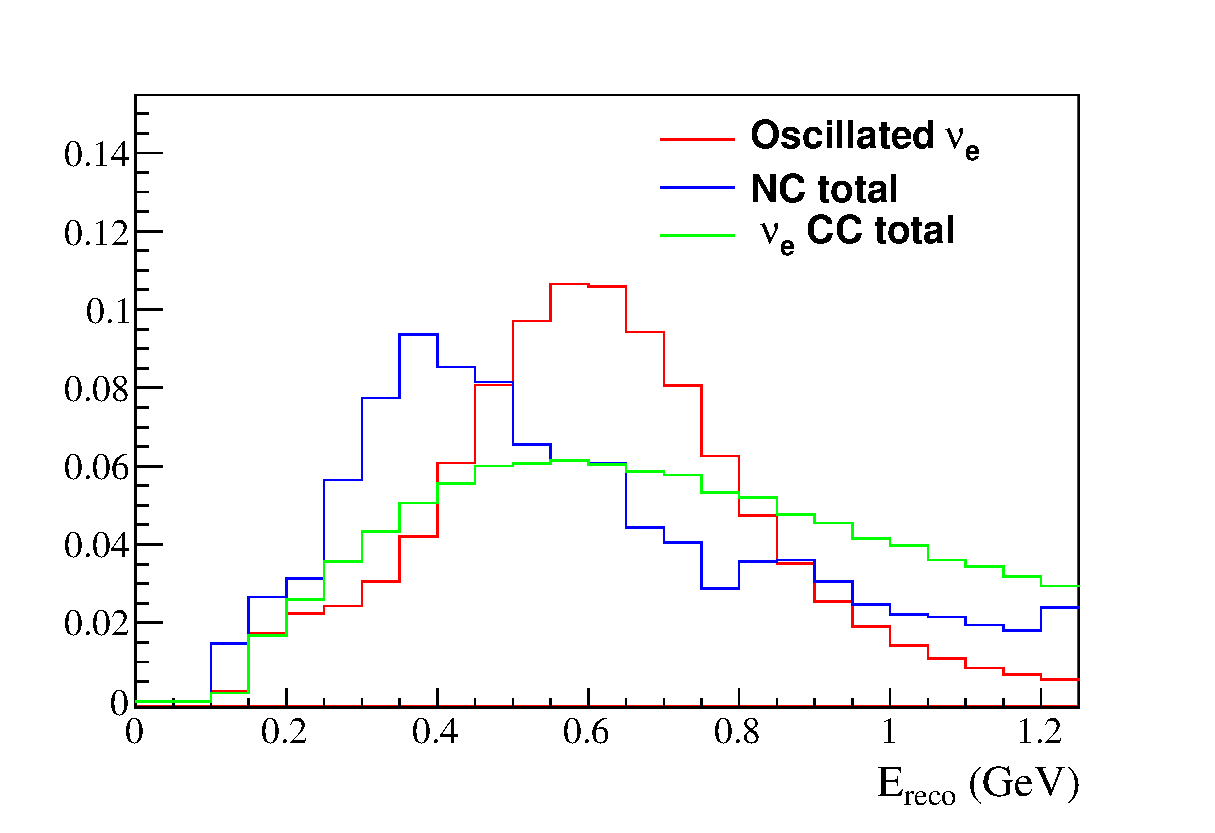
\includegraphics[width=0.5\textwidth]{images/appendix/nue_standalone/ErecoDistForComparisonFig1Nakayama.eps}
\caption{MC predicted reconstructed neutrino energy distribution (area-normalized) for $\nu_{\mu} \rightarrow \nu_{e}$ CC signal (red), intrinsic $\nu_{e}$ CC background (green) 
and NC background (blue) components obtained with {\em VaLOR} framework, using  
$sin^{2}(2\theta_{12}) = 0.8704$, $\Delta m_{21}^{2} = 7.6 \times 10^{-5}$, 
$sin^{2}(2\theta_{23}) =  1.0$, $|\Delta m_{32}^{2}| = 2.4 \times 10^{-3}$, $\delta_{CP} = 0$ and normal hierarchy. }
\label{fig:nueoff1}
\end{center}
\end{figure}

A p-value test similar to the one described in \cite{NueRun123AnalysisEreco} has been performed. 11 $\nu_{e}$ candidates has been observed in the Run1+2+3 data-set. 
The p-value is defined as the probability for observing 11 or more $\nu_{e}$ candidate events in the $3.010 \times 10^{20}$ POT data with the $sin^{2}(2\theta_{13}) = 0$ hypothesis.  
$1 \times 10^{6}$ toy experiments with statistical and systematic variations were created in order to compute that probability. 
Fig.~\ref{fig:nueoffpvalue} shows the distribution of the number of $\nu_{e}$ candidate events observed. 
The p-value, corresponding to the area above 11 (white region), is $\approx 8 \times 10^{-4}$, equivalent to a $\approx 3\sigma$ significance. These values, 
although computed with 100 times less toy experiments, are very close to the ones obtained in \cite{NueRun123AnalysisEreco} 
(p-value = $8.6 \times 10^{-4}$, $3.1\sigma$ significance). 

\begin{figure}[htbp]
\center
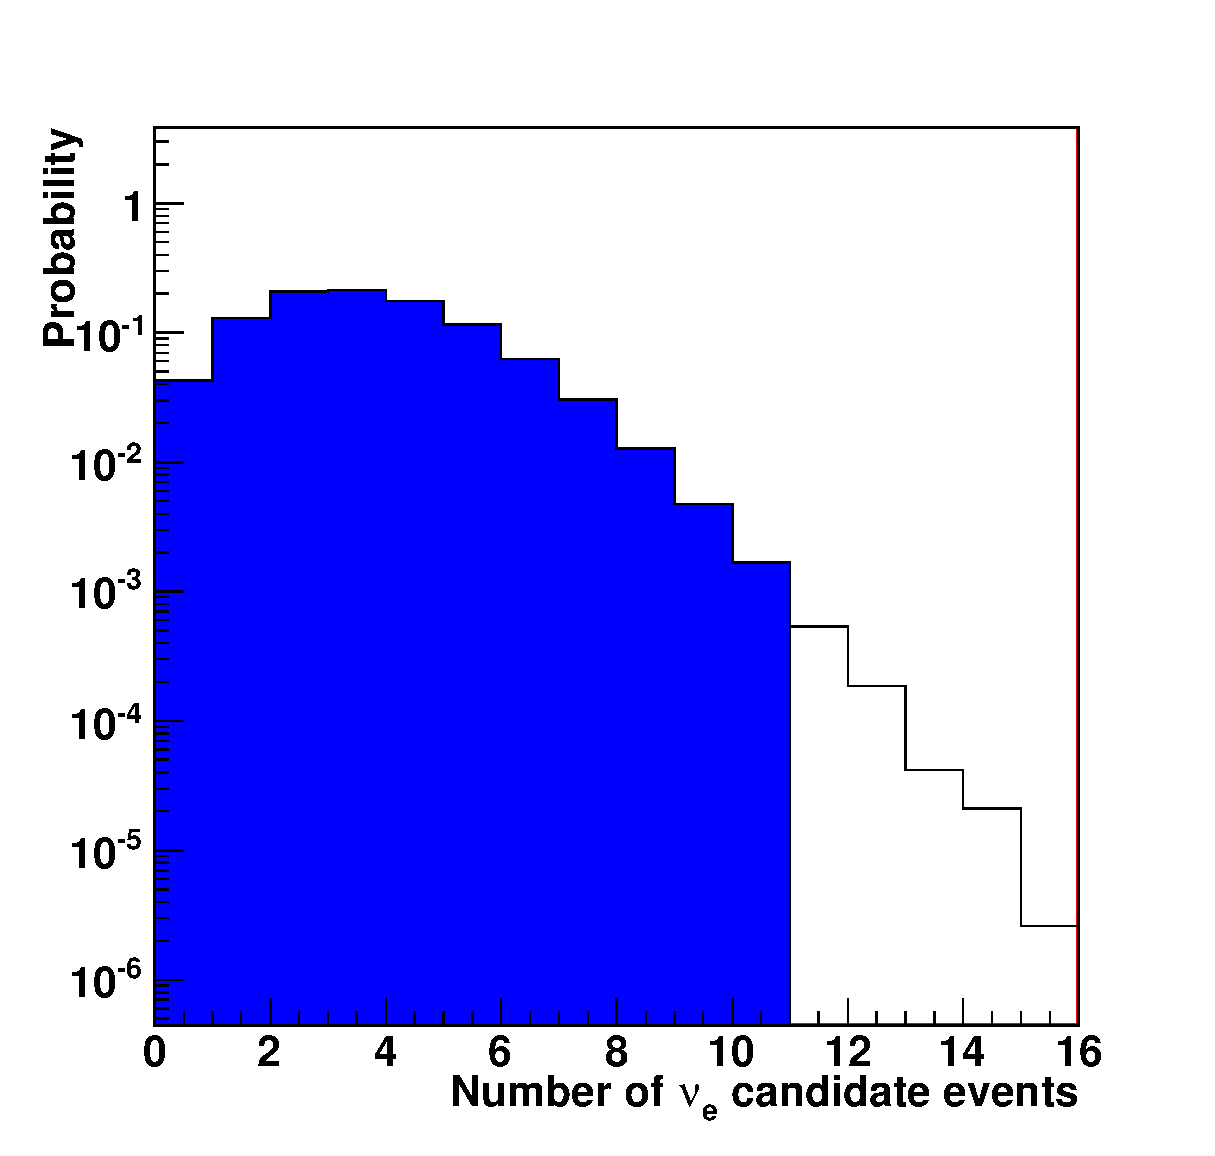
\includegraphics[width=0.5\textwidth]{images/appendix/nue_standalone/PValue.eps}
\caption{ Distribution of predicted number of $nu_{e}$ candidate events over $1\times10^{6}$ toy experiments with $sin^{2}(2\theta_{13}) =  0$, including statistical and systematic variations, for  $3.010 \times 10^{20}$ POT,
$sin^{2}(2\theta_{12}) = 0.8704$, $\Delta m_{21}^{2} = 7.6 \times 10^{-5}$, $sin^{2}(2\theta_{23}) =  1.0$, $|\Delta m_{32}^{2}| = 2.4 \times 10^{-3}$, $\delta_{CP} = 0$ and normal hierarchy. }
\label{fig:nueoffpvalue}
\end{figure}


The fit to the Run1+2+3 data-set is the next step in the validation. Fig.~\ref{fig:nueoff2} shows the $\Delta\chi^{2}$ curve for normal (left) and inverted (right) hierarchy, 
in great agreement with Fig. 20 in \cite{NueRun123AnalysisEreco}.
The corresponding best-fit point and confidence intervals for $sin^{2}(2\theta_{13})$ are summarized in table \ref{tab:nueoff3}. 
Finally, the reconstructed energy spectrum at the best-fit point is presented in Fig.~\ref{fig:nueoff3}, 
which is again in excellent agreement with Fig. 21 in \cite{NueRun123AnalysisEreco}. 

From these comparisons and other detailed tests not shown here, it is concluded that the 2012 {\em VaLOR} stand-alone $\nu_e$-appearance 
analysis gives equivalent results to the T2K official appearance analyses.


\begin{figure}[htbp]
\center
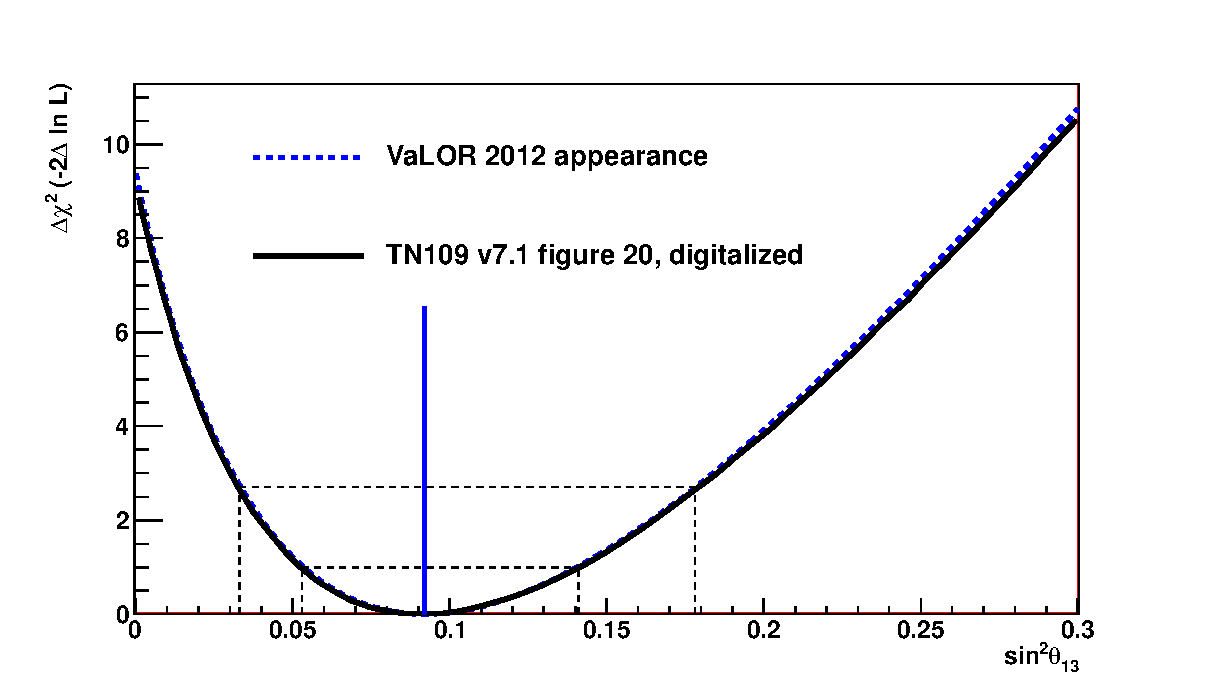
\includegraphics[width=0.5\textwidth]{images/appendix/nue_standalone/OffNue2012DeltaChisqNH.eps}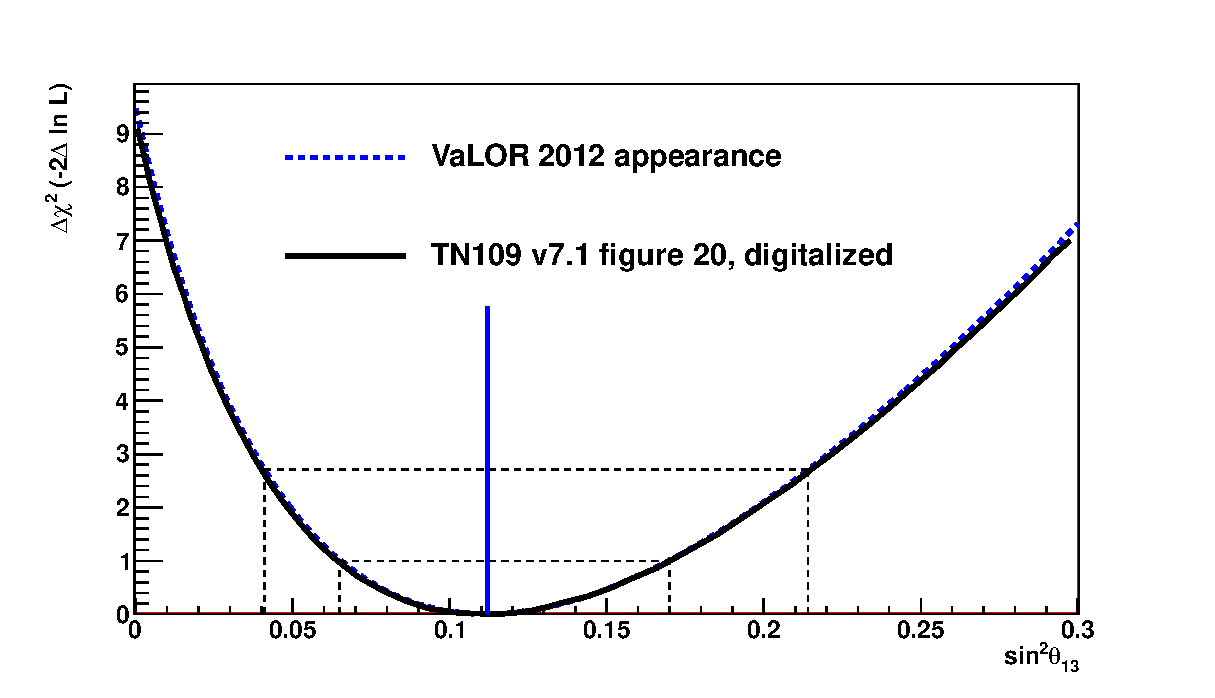
\includegraphics[width=0.5\textwidth]{images/appendix/nue_standalone/OffNue2012DeltaChisqIH.eps}
\caption{$\Delta\chi^{2}$ distribution for the Run1+2+3 data fit assuming normal (left) and inverted (right) mass hierarchy, for 2012 {\em VaLOR} appearance analysis (dashed blue) and 2012 
official results from Fig. 21 in \cite{NueRun123AnalysisEreco} (solid black - digitalized). Fixed values used: $sin^{2}(2\theta_{12}) = 0.8704$, 
$\Delta m_{21}^{2} = 7.6 \times 10^{-5}$, $sin^{2}(2\theta_{23}) =  1.0$, $|\Delta m_{32}^{2}| = 2.4 \times 10^{-3}$ and $\delta_{CP} = 0$.}
\label{fig:nueoff2}
\end{figure}



\begin{table}[htbp]
\center
\begin{tabular}{|c|c|c|c|c|}
\hline 
 & NH (TN109) & NH ({\em VaLOR}) & IH (TN109) & IH ({\em VaLOR}) \\
 \hline \hline
 Best fit & \color{blue}{0.092} & 0.092 & \color{blue}{0.112} & 0.112 \\
  \hline
  68 \% C.L. & \color{blue}{0.053-0.141} & 0.053-0.141&  \color{blue}{ 0.065-0.170} &  0.065 - 0.170\\
  \hline
    90 \% C.L. & \color{blue}{0.033-0.179} & 0.033-0.178 &  \color{blue}{ 0.040-0.215} & 0.041 - 0.214 \\
\hline
\end{tabular}
\caption{Best-fit points and confidence intervals for $sin^{2}(2\theta_{13})$ obtained from Fig.~\ref{fig:nueoff2}, 
with $\delta_{CP} = 0$, $sin^{2}(2\theta_{12}) = 0.8704$, $\Delta m_{21}^{2} = 7.6 \times 10^{-5}$, 
$sin^{2}(2\theta_{23}) =  1.0$ and $|\Delta m_{32}^{2}| = 2.4 \times 10^{-3}$, for normal (NH) and inverted (IH) hierarchy. }
\label{tab:nueoff3}
\end{table}



\begin{figure}[htbp]
\center
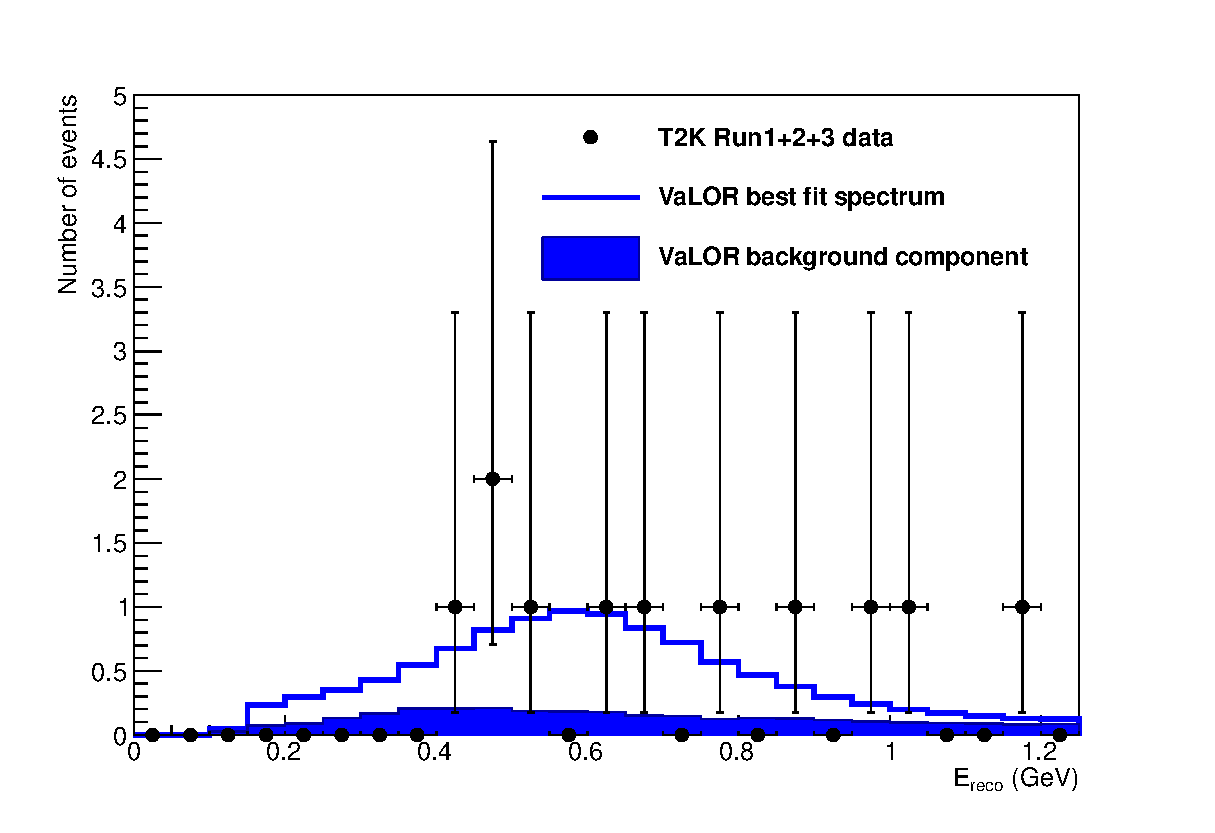
\includegraphics[width=0.5\textwidth]{images/appendix/nue_standalone/BestFitData2012NH.eps}
\caption{Reconstructed energy spectrum at the best-fit point for Run1+2+3 data fit with the {\em VaLOR} 
appearance analysis, 
assuming $\delta_{CP} = 0$, $sin^{2}(2\theta_{12}) = 0.8704$, $\Delta m_{21}^{2} = 7.6 \times 10^{-5}$, $sin^{2}(2\theta_{23}) =  1.0$, $|\Delta m_{32}^{2}| = 2.4 \times 10^{-3}$ and normal hierarchy.}
\label{fig:nueoff3}
\end{figure}




%is presented in Fig.\ \ref{fig:nuecomparison}. 
%The numbers of signal and background events obtained from the two analyses are compared in table \ref{tab:nueoff} 
%for two different values of $\sin^{2}2\theta_{13}$.
%From these comparisons and other detailed tests not shown here, we conclude that the {\em VaLOR} $\nu_e$-appearance 
%analysis gives equivalent results to the T2K official analyses.

%\begin{figure}[htbp]
%\begin{center}
%\includegraphics[width=0.8\textwidth]{images/appendix/ConfidenceContoursNueNormal.eps}
%\caption{Comparison of 90\% (blue) and 68\% (red) C.L. contours from the T2K official $\nu_{e}$-appearance analysis \cite{NueRun1and2Analysis} 
    %    (dashed lines, light colors) with those obtained with the {\em VaLOR} $\nu_{e}$-appearance analysis (solid lines, dark colors). The {\em VaLOR} 
        %contours are in good agreement with those from the  official analysis; the small differences are due to the limited number of 
        %Feldman-Cousins jobs run for this comparison.}
%\label{fig:nuecomparison}
%\end{center}
%\end{figure}

%\begin{table}[h]
%\centering
%\begin{tabular}{|c|c|c|c|c|}
%\hline
 % & \multicolumn{2}{|c|}{$\sin^{2}2\theta_{23}$ = 0} & \multicolumn{2}{|c|}{$\sin^{2}2\theta_{23}$ = 0.1} \\
%\cline{2-5}
 % & T2K official & {\em VaLOR}  & T2K official & {\em VaLOR} \\
%\hline \hline
%Beam total & 1.40 & 1.44 & 1.34 & 1.37 \\
%\hline
%Beam $\nu_{\mu}$ and $\bar{\nu_{\mu}}$ CC  & 0.03 & 0.03 & 0.03 & 0.03 \\
%Beam $\nu_{e}$ CC  & 0.76 & 0.77 & 0.70 & 0.71 \\
%all NC  & 0.61 & 0.63 & 0.61 & 0.63 \\
%\hline
%Signal $\nu_{\mu}\rightarrow\nu_{e}$  & 0.09 & 0.09 & 4.11 & 4.18 \\
%\hline
%Total & 1.49 & 1.53 & 5.45 & 5.55 \\
%\hline
%\end{tabular}
%\caption{Comparison of numbers of $\nu_{e}$ events in SuperK at $\sin^{2}2\theta_{13}=0$ and $\sin^{2}2\theta_{13}=0.1$ between the T2K 
   %      official analysis \cite{NueRun1and2Analysis} and the {\em VaLOR} stand-alone $\nu_{e}$-appearance analysis.}
%\label{tab:nueoff}
%\end{table}



% continuation of the analyses performed by the same group on the 2-flavour $\nu_{\mu}$-disappearance framework described in Ref. \cite{OurRun1and2Analysis2F}, \cite{OurRun1DisappAnalysis2F}. The different inputs used for this joint oscillation analysis, corresponding to the T2K 2010 analysis, that are not specified in this section are described in Ref. \cite{OurRun1and2Analysis2F} and \cite{OurRun1DisappAnalysis2F}.

% A full 3-flavour framework with matter effects was implemented by the Rutherford-Oxford-Lancs group as reported in Ref. \cite{OurRun1and2Analysis3F}. In the same framework, the elements to build also the $\nu_{e}$-appearance analysis were included, following the descriptions in Ref.\cite{NueRun1and2Analysis}, becoming the {\em VaLOR} framework for the joint oscillation analysis which handles the 1R$\mu$ sample and the 1Re sample at the same time. Details about the stand-alone appearance and disappearance analyses combined for the joint analysis will be described in this section.

% \subsection{Event selection cuts}

% The nominal SuperK one ring e-like and $\mu$-like MC templates are constructed by applying the one ring e-like or $\mu$-like selection cuts on the official SuperK MC samples. The \textbf{one ring e-like selection cuts} correspond to the official 2010 cuts that can be summarized as follows:

% \begin{enumerate}
% \item{Fully contained: the number of PMT hits in highest-charge OD cluster is less than 16. }
% \item{Fiducial volume: the reconstructed vertex is at least 2m away from ID wall.}
% \item{Visible energy cut: the visible energy in the event is above 100 MeV ($E_{vis}>100MeV$).}
% \item{One ring cut: there is only one reconstructed ring in the event.}
% \item{PID cut: the reconstructed ring is e-like (ip[0]=2).}
% \item{Michel electron cut: the number of decay electrons must be 0.}
% \item{Pi0 mass cut: the invariant mass calculated with forced second ring is less than 105MeV ($M_{inv}<105 MeV$).}
% \item{Reconstructed neutrino energy cut: the reconstructed neutrino energy is less than 1250 MeV ($E_{\nu}^{reco}<1250MeV$).}
% \end{enumerate}

% The \textbf{one ring $\mu$-like selection cuts} also correspond to the official 2010 cuts and are the following ones:

% \begin{enumerate}
% \item{Fully contained: the number of PMT hits in highest-charge OD cluster is less than 16. }
% \item{Fiducial volume: the reconstructed vertex is at least 2m away from ID wall.}
% \item{Visible energy cut: the visible energy in the event is above 30 MeV ($E_{vis}>30MeV$).}
% \item{One ring cut: there is only one reconstructed ring in the event.}
% \item{PID cut: the reconstructed ring is $\mu$-like (ip[0]=3).}
% \item{Muon momentum cut: the momentum reconstructed as muon must be larger than 200 MeV (amomm[0]$>$200MeV)}
% \item{Michel electron cut: the number of decay electrons must be no larger than one ($<=1$ decay $e^{-}$).}
% \end{enumerate}


% \subsection{SK MC templates and prediction}

% For the new \textbf{1R$_{e}$-like sample} the following NEUT interaction modes were included: 

% \begin{enumerate}
% \item{CCQE, CC1$\pi$, CC coh and CC other for $\nu_{\mu}$, $\overline{\nu_{\mu}}$ and $\nu_{e}$}
% \item{NC1$\pi$0, NC coh and NC other for $\nu_{\mu}$, $\overline{\nu_{\mu}}$ and $\nu_{e}$}
% \item{ CCQE, CC1$\pi$ and CC other for signal $\nu_{e}$}
% \end{enumerate}

%  The interaction modes used for the \textbf{1R$_{\mu}$-like sample} were: 
%  \begin{enumerate}
%  \item{CCQE, CC1$\pi$, CC other and NC for $\nu_{\mu}$, $\overline{\nu_{\mu}}$ and $\nu_{e}$}
%  \item{ CCQE, CC1$\pi$ and CC other for signal $\nu_{e}$}
%  \end{enumerate}
 
% In general, the NC modes for signal $\nu_{e}$ are not used, and the NC modes for the rest of flavours are not oscillated (oscillation probabilities set to 1 for them). Notice that the CC other definition is different for the 1R$_{\mu}$ and 1R$_{e}$ samples: in the 1R$_{\mu}$ the CC coh. mode is included in the CC other category while for 1R$_{e}$ is not. The list of interaction modes considered will be updated in next joint analysis, with 2012 upgrades.
 
% For the mu-like sample the $E_{reco}$ spectrum will be used, while for the e-like sample only the number of events (the integral of the $E_{reco}$ spectrum) will be used. In both cases, the steps to construct the SK prediction from the SK MC templates just defined can be summarized as follows:

% \begin{enumerate}
% \item The SK MC files contain for the events passing all cuts previously defined a small ntuple with the following variables : reconstructed energy (erec or EnuReco), generator interaction mode, neutrino true energy (Etrue or inu) and the flavour identification (pdg or ipnu).
% \item With this SK MC files, for each neutrino flavour and mode a SK MC template is filled with the number of events in two dimensional ($E_{reco}$,$E_{true}$) bins. 
% \item A first reweighting is applied to these samples: the number of events is weighted in each ($E_{reco}$,$E_{true}$) bin by (data POT / MC POT) depending on the interaction mode and neutrino flavour.
% \item Then, multiplicative systematic errors are applied to all templates, reweighting the number of events in each ($E_{reco}$,$E_{true}$) bin. These multiplicative systematics can be dependent on the neutrino true or reconstructed energy and they are: flux shape, efficiencies, cross sections and FSI systematics. The flux reweighting (flux version 10a $\rightarrow$ 10d) is applied along with these systematic errors. 
% \item With all multiplicative systematic errors included now the reconstructed energy scale systematic is applied to all templates. This systematic error is applied scaling the edges of the $E_{reco}$ bins and calculating the number of events that each bin has gained and/or lost from adjacent bins assuming a uniform distribution of events in each bin.
% \item Now the neutrino oscillations are applied to the templates with systematics already included. The oscillation probabilities are calculated for the different neutrino flavours depending on the true neutrino energy and the input value of the oscillation parameters, and then applied to the corresponding template (according to its flavour) and ($E_{reco}$,$E_{true}$) bin. 
% \item Finally a sum over all $E_{true}$ bins is performed in each template to construct the $E_{reco}$ spectrum for each neutrino flavour and mode. 
% \item A total $E_{reco}$ spectrum is built adding the content in the same $E_{reco}$  bin for all modes and flavours histograms. The number of events for the 1R$_{e}$-like sample is the integral of the total $E_{reco}$ spectrum.
%  \end{enumerate} 

% \subsection{Systematic errors}

% For the $\nu_{\mu}$-disappearance analysis, the list of systematic errors included in the analysis, described in Ref. \cite{OurRun1and2Analysis2F} and  \cite{OurRun1DisappAnalysis2F}, is the following:

% \begin{enumerate}
% \item SuperK CCQE efficiency
% \item SuperK CCnonQE efficiency
% \item SuperK NC efficiency
% \item Super $\nu_{e}$ CC efificiency
% \item SuperK ring counting
% \item ND280 efficiency
% \item Flux normalization
% \item Flux shape
% \item FSI
% \item SuperK energy scale
% \item CCQE cross section
% \item CC$1\pi$/CCQE cross section ratio
% \item NC/CCQE cross section ratio
% \item CCother/CCQE cross section ratio
% \item NC/CCQE cross section ratio
% \end{enumerate}

% Some of the systematics already mentioned at fully correlated for both the one ring e-like and one ring $\mu$-like samples so they are common for both of them in the joint oscillation analysis:

% \begin{enumerate}
% \item SuperK ring counting
% \item SuperK energy scale
% \item CCQE cross section
% \item CC$1\pi$/CCQE cross section ratio
% \item CCother/CCQE cross section ratio
% \item FSI
% \item ND280 normalization
% \item Flux normalization
% \end{enumerate}

% Additionally to the systematic uncertainties already mentioned, several other systematic parameters only related to the one ring e-like sample were included. They can be summarized as follows:

% \begin{enumerate}
% \item 1Re-like signal SuperK efficiency 
% \item 1Re-like background SuperK efficiency 
% \item CC coh. to CCQE cross section 
% \item NC 1$\pi^{0}$ to CCQE cross section 
% \item NC coh. to CCQE cross section
% \item NC other to CCQE cross section 
% \item $\nu_{e}$ to $\nu_{\mu}$ cross section
% \end{enumerate}

% The uncertainties on the cross sections were provided by the NIWG and are obtained from the version file niwg\_errors\_10a\_v1.root.
% One sigma uncertainties of the systematic parameters related to SuperK detector efficiency for signal (1.4\%) and background (1.4\%) events are taken from \cite{NueRun1and2Analysis}, coming in turn from Table 24 in \cite{TN28}.
% The effect of specific systematics for the $\nu_{e}$-appearance analysis introduced was checked in comparison with the results available (in Ref. \cite{NueRun1and2Analysis}, table 3).


% \subsection{Validation of the stand-alone appearance analysis}

% Once the updates and additions were introduced and operative, the first natural step was to reproduce the official results for the $\nu_{e}$-appearance contours reported in Ref.\cite{NueRun1and2Analysis}. Figure \ref{fig:nuecomparison} shows the comparison of the 68\% and 90\% C.L. contours of the $\nu_{e}$-appearance analysis done with the framework used in this work and the official results, taken from \cite{OfficialNueAnalysisCodeT2KWebsite}. The preliminary results are in very good agreement with the official analysis, small differences appear due to the limited number of Feldman-Cousins jobs \cite{FeldmanCousins} run for this comparison intended to be a quick check. Table \ref{tab:nueoff} shows a comparison between the number of events at $sin^{2}2\theta_{13}=0$ and $sin^{2}2\theta_{13}=0.1$ for the different beam components and signal for the official analysis (taken from Table 16 in \cite{NueRun1and2Analysis}) and the stand-alone study done for this work. 

% \begin{figure}[htbp]
% \begin{center}
% \includegraphics[width=0.8\textwidth]{images/appendix/ConfidenceContoursNueNormal.eps}
% \caption{Comparison of 90\% (blue) and 68\% (red) C.L. contours for the official $\nu_{e}$-appearance analysis \cite{NueRun1and2Analysis} (dashed, light colors)  and the ones obtained with the framework used in this work (solid, dark colors). The new contours are in good agreement with the official ones, small differences appear due to the limited number of FC jobs run for this comparison.}
% \label{fig:nuecomparison}
% \end{center}
% \end{figure}

% \begin{table}[h]
% \centering
% \begin{tabular}{|c|c|c|c|c|}
% \hline
%   & $sin^{2}2\theta_{23}=0$ official & $sin^{2}2\theta_{23}=0$ & $sin^{2}2\theta_{23}=0.1$ official & $sin^{2}2\theta_{23}=0.1$\\
% \hline \hline
% Beam total & 1.40 & 1.44 & 1.34 & 1.37 \\
% \hline
% Beam $\nu_{\mu}$ and $\bar{\nu_{\mu}}$ CC  & 0.03 & 0.03 & 0.03 & 0.03 \\
% Beam $\nu_{e}$ CC  & 0.76 & 0.77 & 0.70 & 0.71 \\
% all NC  & 0.61 & 0.63 & 0.61 & 0.63 \\
% \hline
% Signal $\nu_{\mu}\rightarrow\nu_{e}$  & 0.09 & 0.09 & 4.11 & 4.18 \\
% \hline
% Total & 1.49 & 1.53 & 5.45 & 5.55 \\
% \hline
% \end{tabular}
% \caption{ Comparison of number of events at $sin^{2}2\theta_{13}=0$ and $sin^{2}2\theta_{13}=0.1$ for the different beam components and signal for the official analysis and the stand-alone study done for this work. }
% \label{tab:nueoff}
% \end{table}



\clearpage

\section{Fitter performance. Study of residuals.}
\label{app:fitter_performance}

The fitter performance has been evaluated for different configurations: oscillation points, number of POT, levels 
of throwing systematics and fitters were varied. Residual distributions (best fit value - input value)  are 
presented in this section. For each study, 1000 toy datasets were created and fitted using MINUIT 
(MIGRAD), as explained in Sec.\ \ref{sec:neutrino_oscillation_fitting}. Table \ref{tab:osc_points} shows the true input values of the 
oscillation parameters for the different oscillation points studied. 

\begin{table}[htb]
\centering
\begin{tabular}{| c | c  c  c  c  c |}
\hline
Oscillation point &   $|\Delta m^2|$ (eV$^{2}$/c$^{4}$) & sin$^2\theta_{23}$ & sin$^2\theta_{13}$  & $\delta_{CP}$ & Mass Hierarchy \\
\hline
0  & 2.36 & 0.5 & 0.025 & 0 & NH\\
\hline
1  & 2.36 & 0.38 & 0.025 & 0 & NH\\
\hline
2  & 2.36 & 0.62 & 0.025 & 0 & NH\\
\hline
3  & 2.36 & 0.5 & 0.015 & 0 & NH\\
\hline
4  & 2.36 & 0.5 & 0.035 & 0 & NH\\
\hline
5  & 2.36 & 0.5 & 0.025 & $-\frac{\pi}{2}$ & NH\\
\hline
6  & 2.36 & 0.5 & 0.025 & $\frac{\pi}{2}$ & NH \\
\hline
7  & 2.2 & 0.5 & 0.025 & 0 & NH \\
\hline
8  & 2.8 & 0.5 & 0.025 & 0 & NH \\
\hline
9  & 2.36 & 0.5 & 0.025 & 0 & IH\\
\hline
\end{tabular}
\caption{
  True input values for the different oscillation points used in the study of fitter performance.
}
\label{tab:osc_points}
\end{table}


\subsection{'4 + 0' fit}

Figs. \ref{fig:residuals_40_first} - \ref{fig:residuals_40_last} show the distribution of residuals of the four 
oscillation parameters for each set described in table \ref{tab:osc_points} at $3.010 \times 10^{20}$ POT.
The distribution of residuals for $\delta_{CP}$ should not be taken into account due to the insensitivity to this parameter at current POT. 
A pileup similar to the one observed at maximal  mixing $sin^{2}(2\theta_{23}) = 1.0$ in the stand-alone disappearance 
analysis is now appearing at the center of symmetry of the P($\nu_{\mu}\rightarrow\nu_{\mu}$) curve,
which corresponds with the maximal disappearance (the difference between $sin^{2}(\theta_{23})$ values for maximal disappearance and
maximal mixing is explained in Sec. \ref{app:symmetry}).
This pile-up is reduced when the input value for $sin^{2}(\theta_{23})$ is far from 0.5 
(see figures  \ref{fig:residuals_40_point1} and  \ref{fig:residuals_40_point2}) and disappears if the 
POT is increased, as shown in figure \ref{fig:residuals_40_point1_x100}.
In general there are no unexpected features.

\clearpage

\begin{figure*}[htb]
\begin{minipage}[t]{0.5\linewidth}
\center
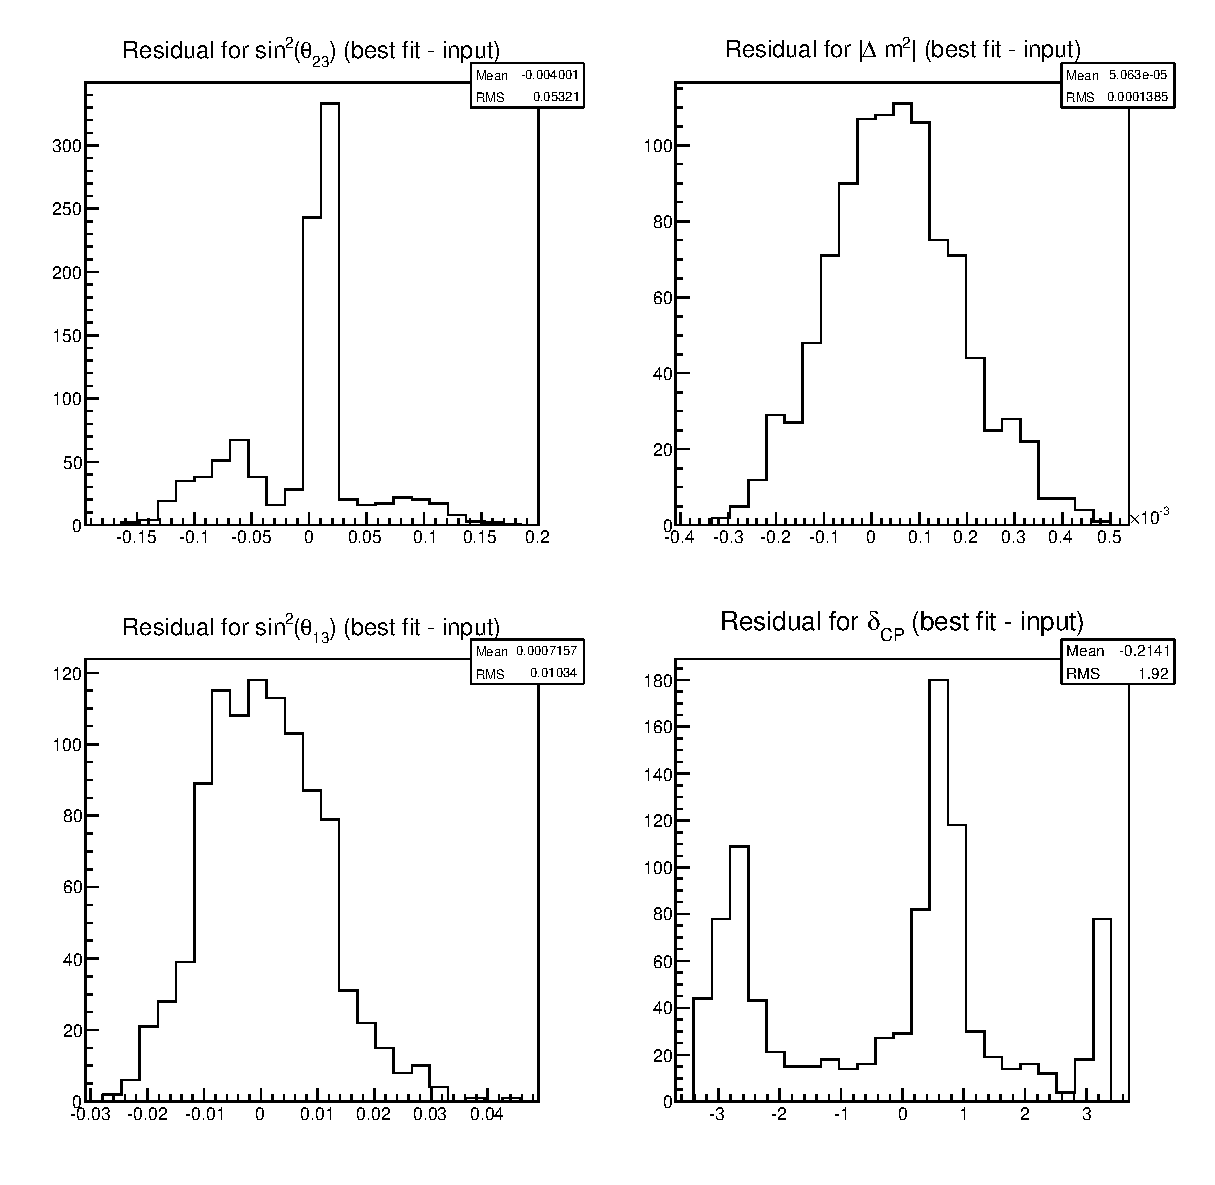
\includegraphics[width=18pc]{images/appendix/fitter_performance/Osc_residuals_nosyst_point0.eps}
\caption{
	Distribution of residuals of the four oscillation parameters in the '4 + 0' fit for oscillation point \# 0. 
 }
\label{fig:residuals_40_first}
\end{minipage}
\hspace{0.02\linewidth}
\begin{minipage}[t]{0.5\linewidth}
\center
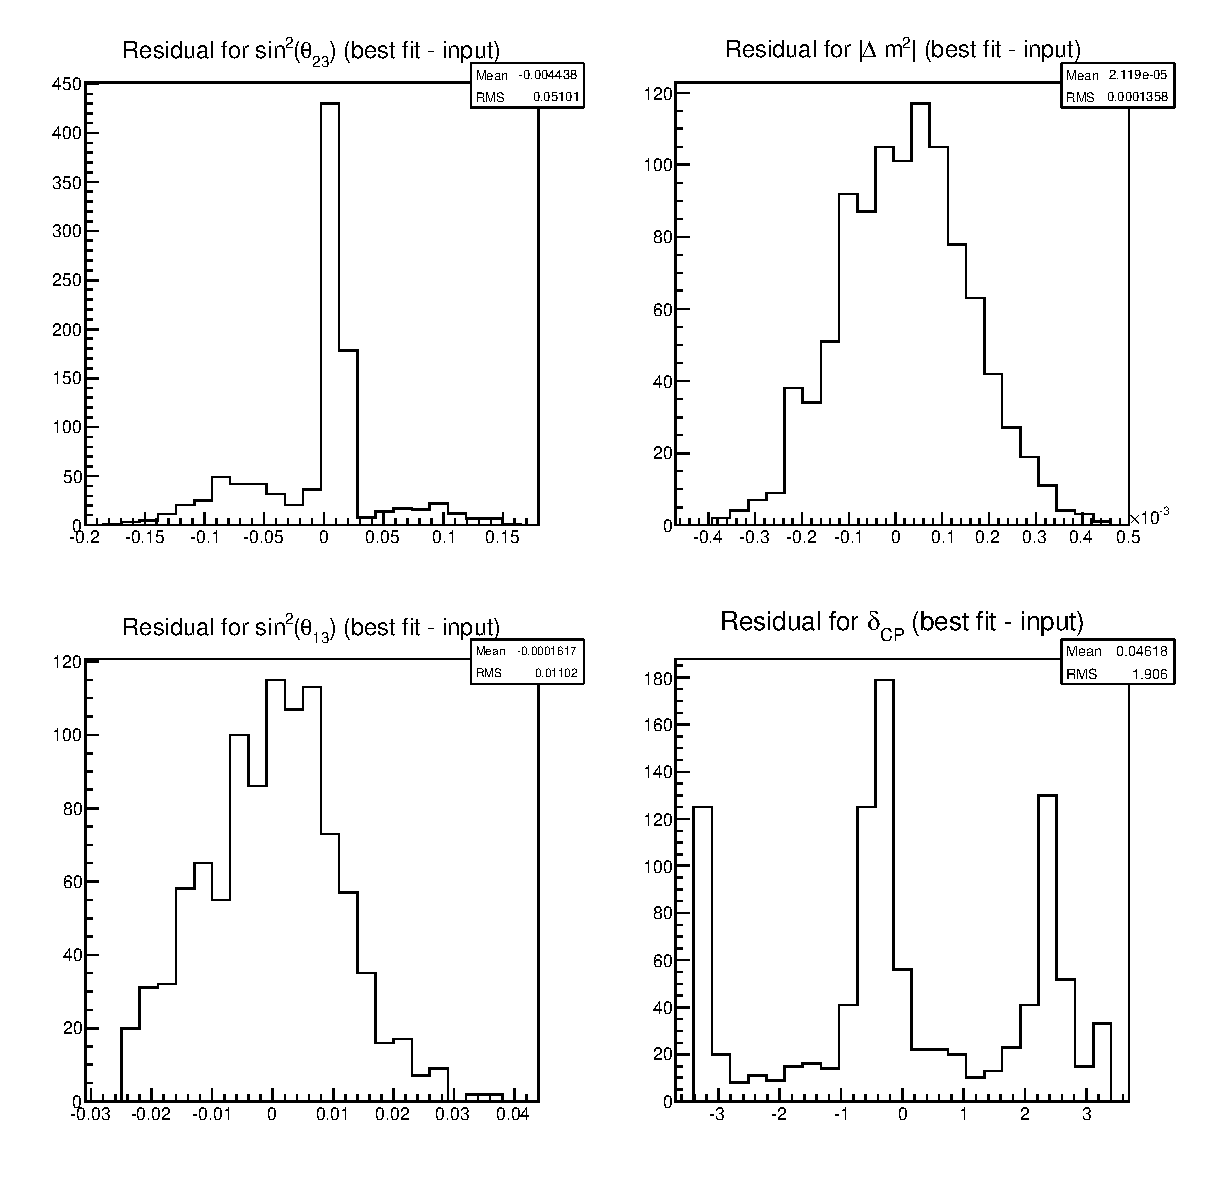
\includegraphics[width=18pc]{images/appendix/fitter_performance/Osc_residuals_nosyst_point9.eps}
\caption{
	Distribution of residuals of the four oscillation parameters in the '4 + 0' fit for oscillation point \# 9. 
 }
\end{minipage}

\end{figure*}


\begin{figure*}[htb]
\begin{minipage}[t]{0.5\linewidth}
\center
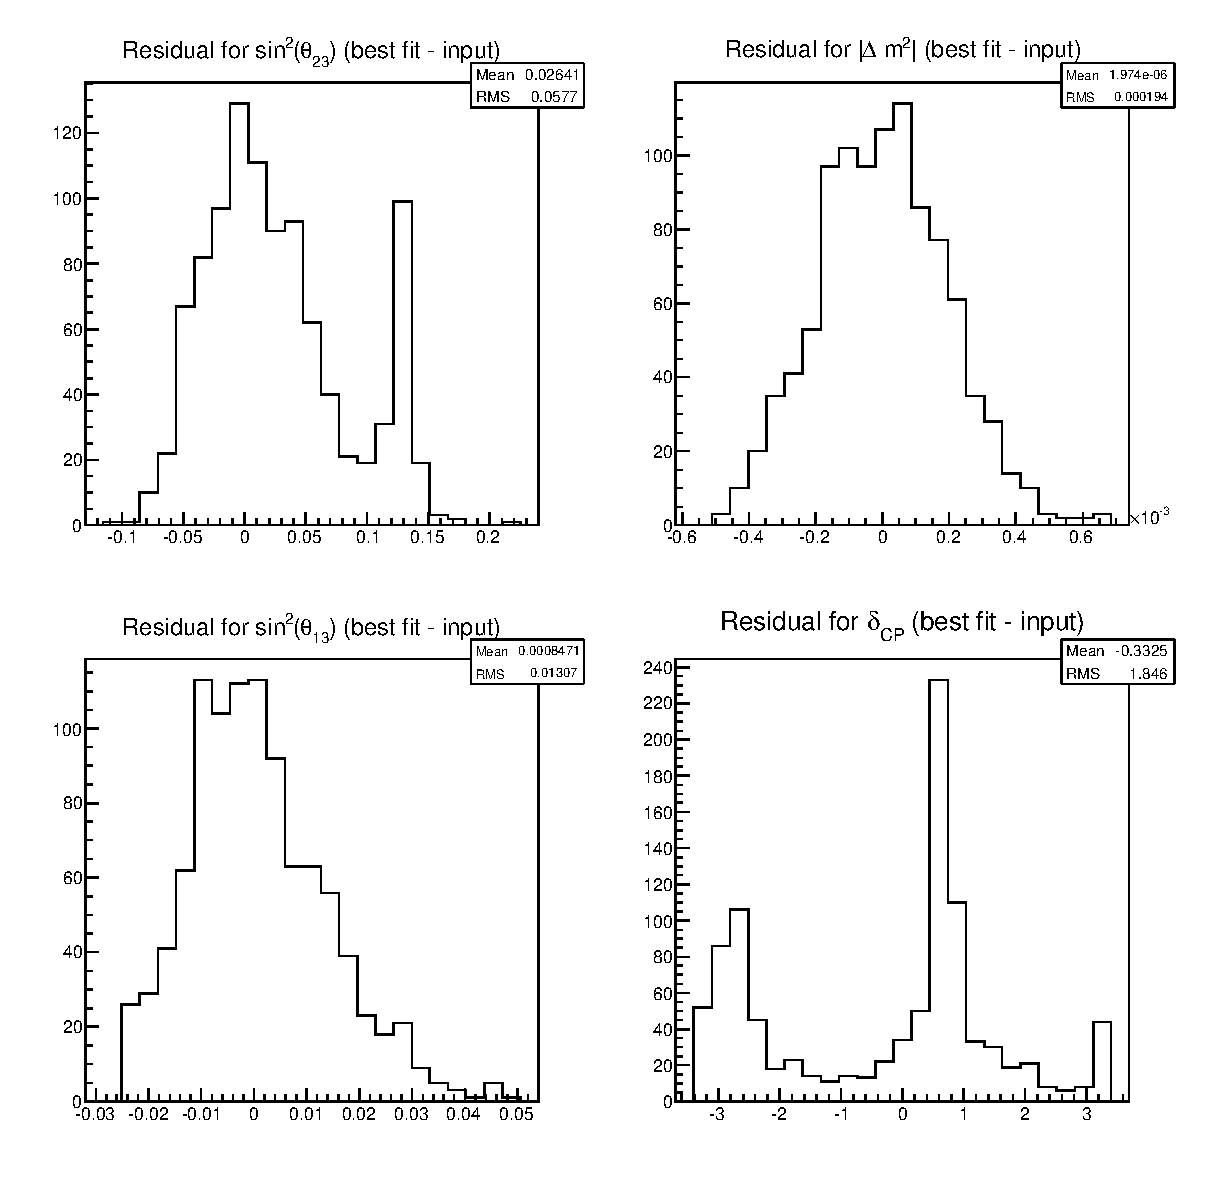
\includegraphics[width=18pc]{images/appendix/fitter_performance/Osc_residuals_nosyst_point1.eps}
\caption{
	Distribution of residuals of the four oscillation parameters in the '4 + 0' fit for oscillation point \# 1. 
 }
\label{fig:residuals_40_point1}
\end{minipage}
\hspace{0.02\linewidth}
\begin{minipage}[t]{0.5\linewidth}
\center
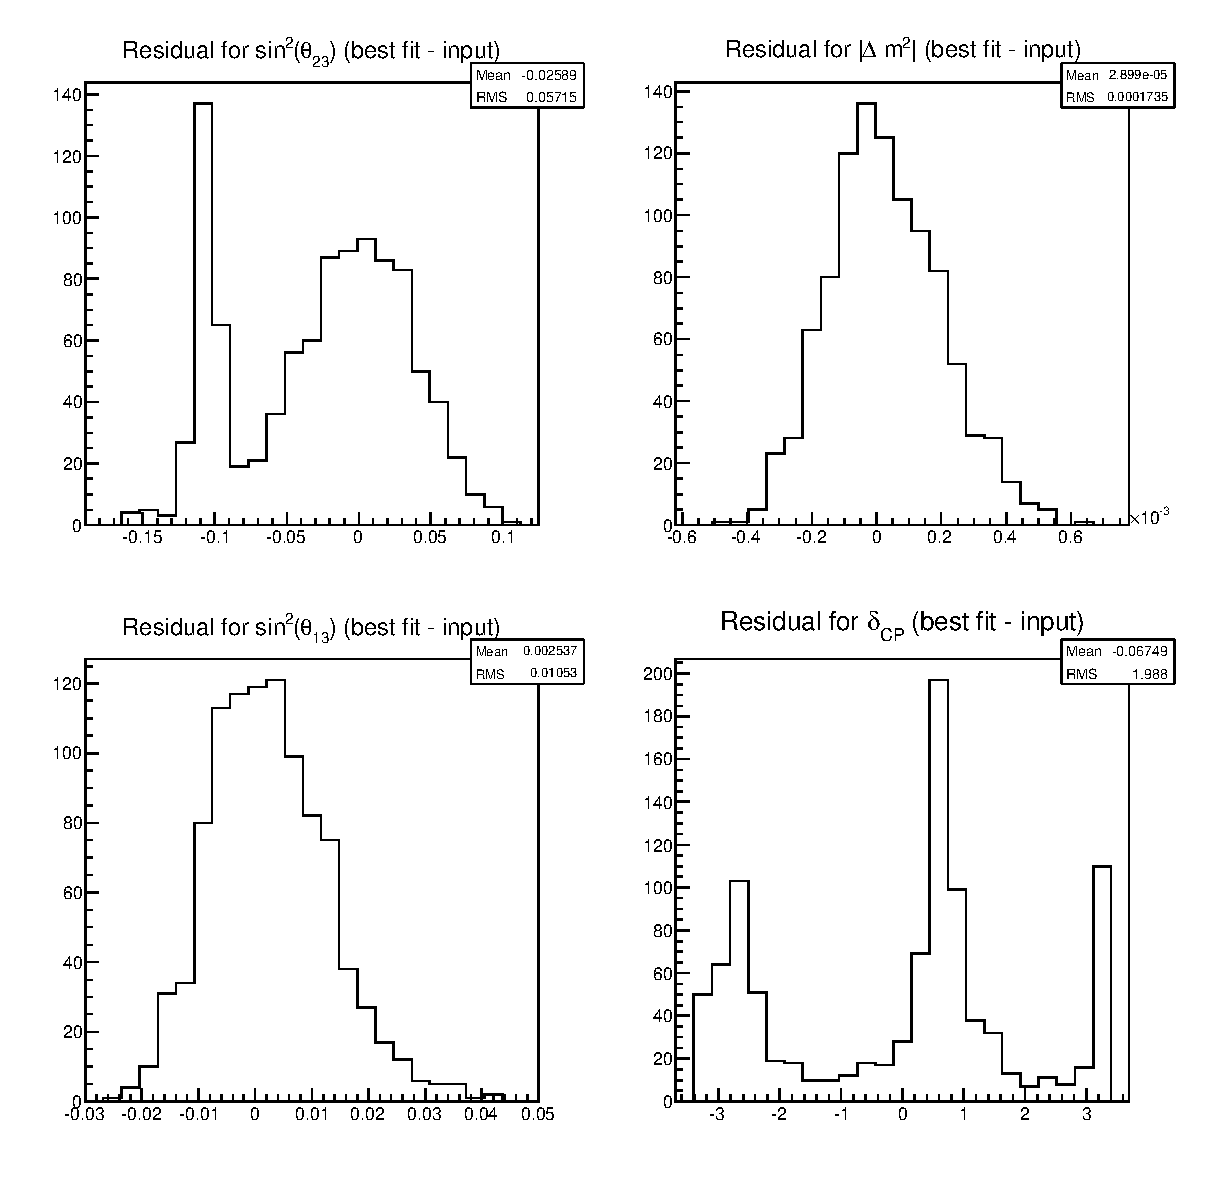
\includegraphics[width=18pc]{images/appendix/fitter_performance/Osc_residuals_nosyst_point2.eps}
\caption{
	Distribution of residuals of the four oscillation parameters in the '4 + 0' fit for oscillation point \# 2. 
 }
\label{fig:residuals_40_point2}
\end{minipage}
\end{figure*}
\clearpage

\begin{figure*}[htb]
\begin{minipage}[t]{0.5\linewidth}
\center
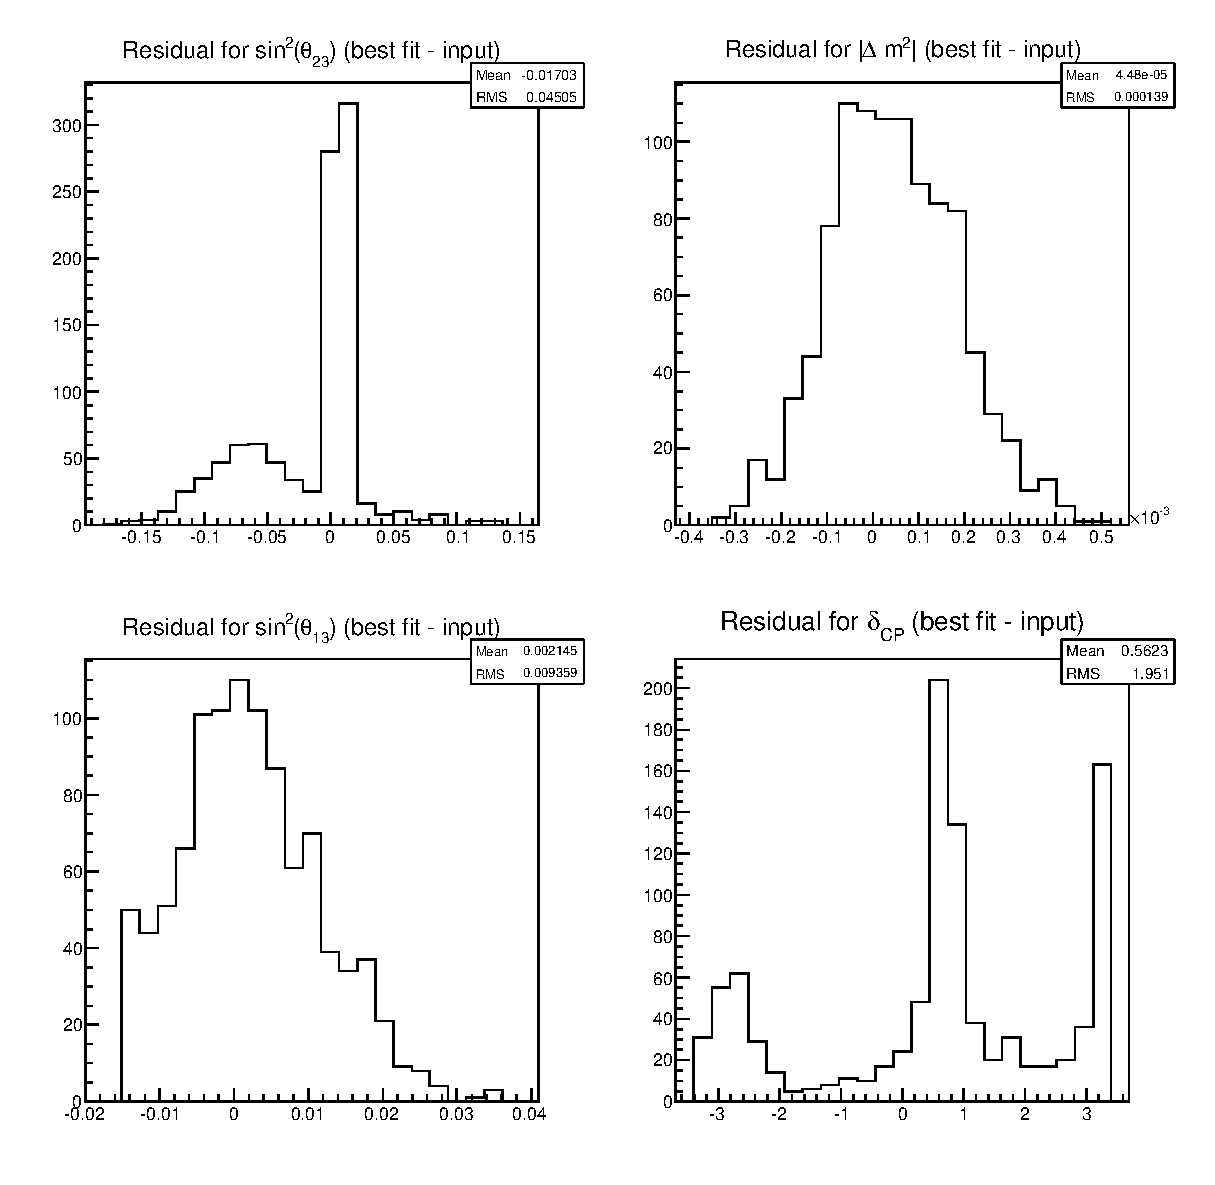
\includegraphics[width=18pc]{images/appendix/fitter_performance/Osc_residuals_nosyst_point3.eps}
\caption{
	Distribution of residuals of the four oscillation parameters in the '4 + 0' fit for oscillation point \# 3. 
 }
\label{fig:residuals_40_point3}
\end{minipage}
\hspace{0.02\linewidth}
\begin{minipage}[t]{0.5\linewidth}
\center
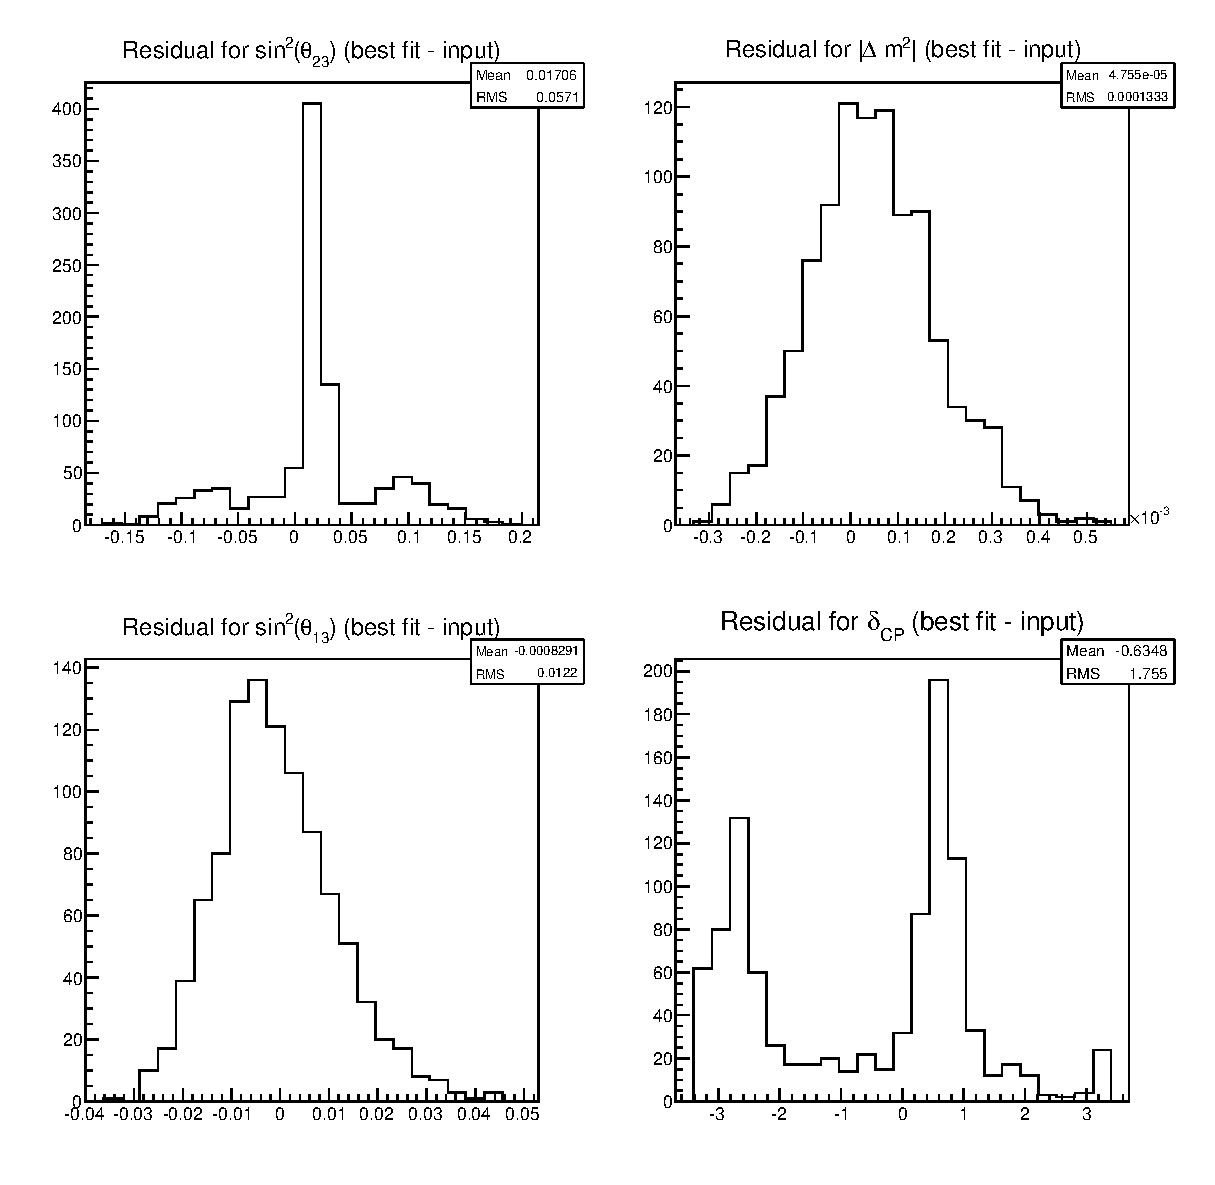
\includegraphics[width=18pc]{images/appendix/fitter_performance/Osc_residuals_nosyst_point4.eps}
\caption{
	Distribution of residuals of the four oscillation parameters in the '4 + 0' fit for oscillation point \# 4. 
 }
\end{minipage}

\end{figure*}


\begin{figure*}[htb]
\begin{minipage}[t]{0.5\linewidth}
\center
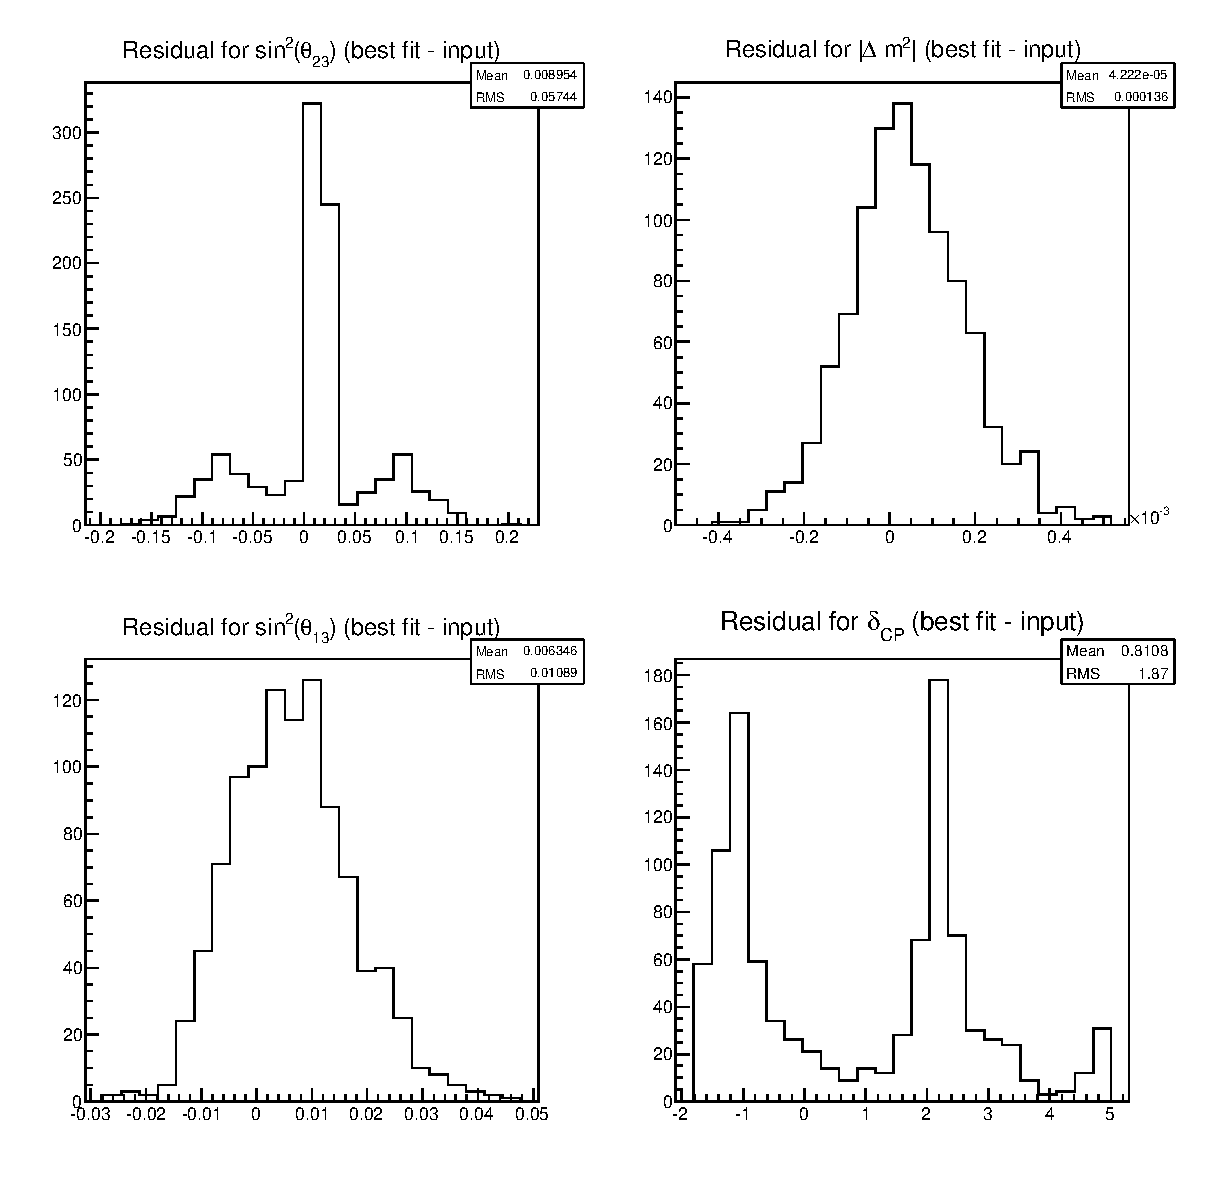
\includegraphics[width=18pc]{images/appendix/fitter_performance/Osc_residuals_nosyst_point5.eps}
\caption{
	Distribution of residuals of the four oscillation parameters in the '4 + 0' fit for oscillation point \# 5. 
 }
\label{fig:residuals_40_point5}
\end{minipage}
\hspace{0.02\linewidth}
\begin{minipage}[t]{0.5\linewidth}
\center
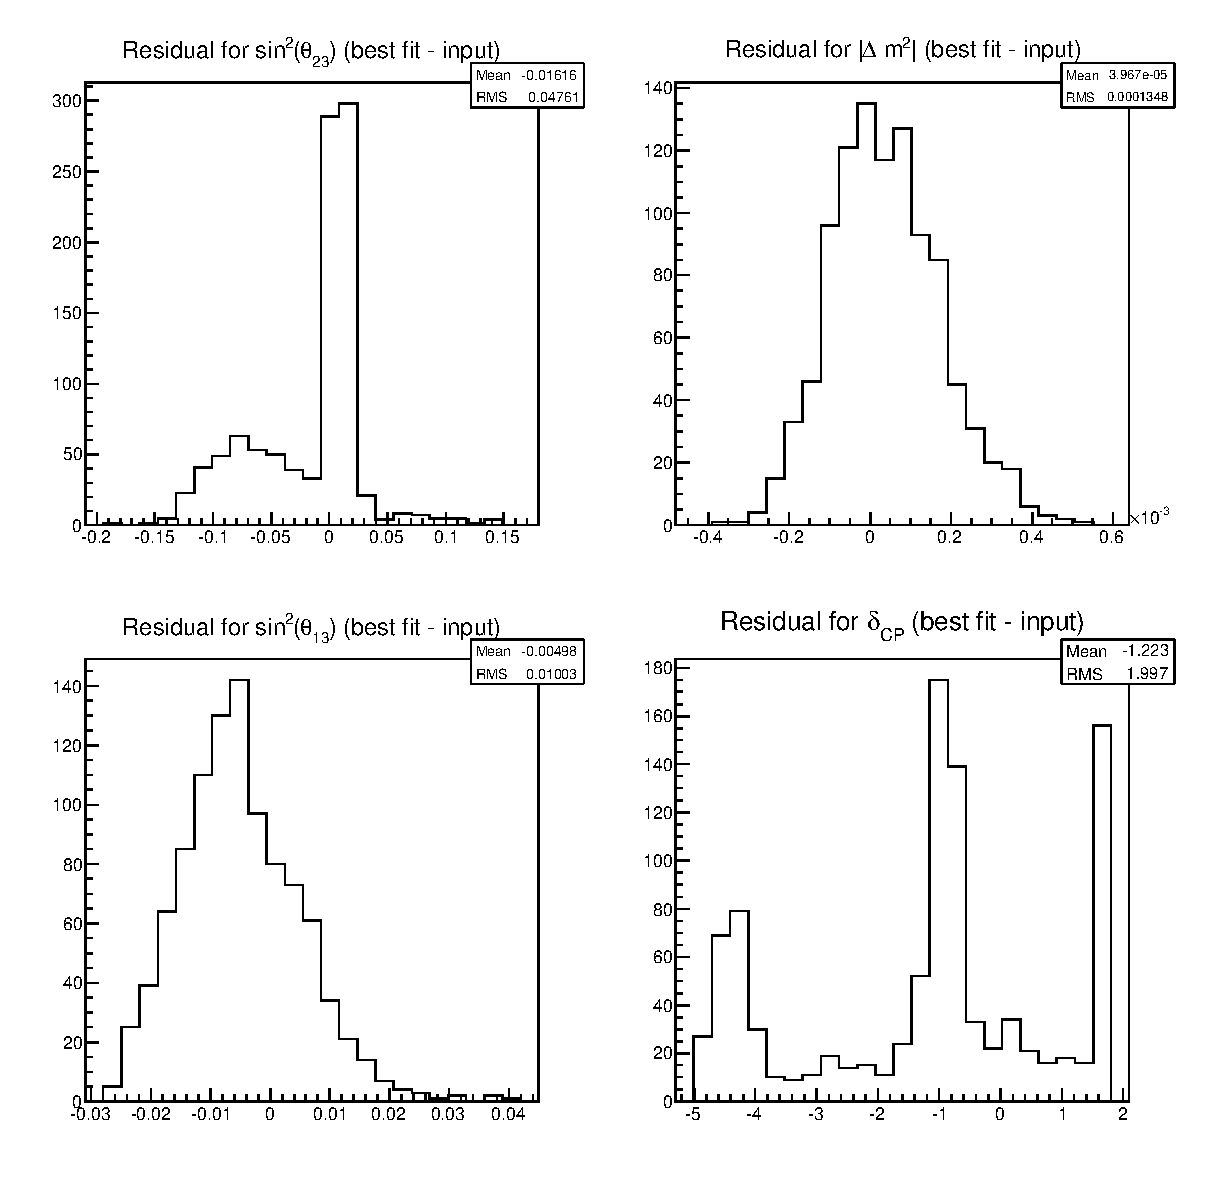
\includegraphics[width=18pc]{images/appendix/fitter_performance/Osc_residuals_nosyst_point6.eps}
\caption{
	Distribution of residuals of the four oscillation parameters in the '4 + 0' fit for oscillation point \# 6. 
 }
 \label{fig:residuals_40_point6}	
\end{minipage}

\end{figure*}

\clearpage

\begin{figure*}[htb]
\begin{minipage}[t]{0.5\linewidth}
\center
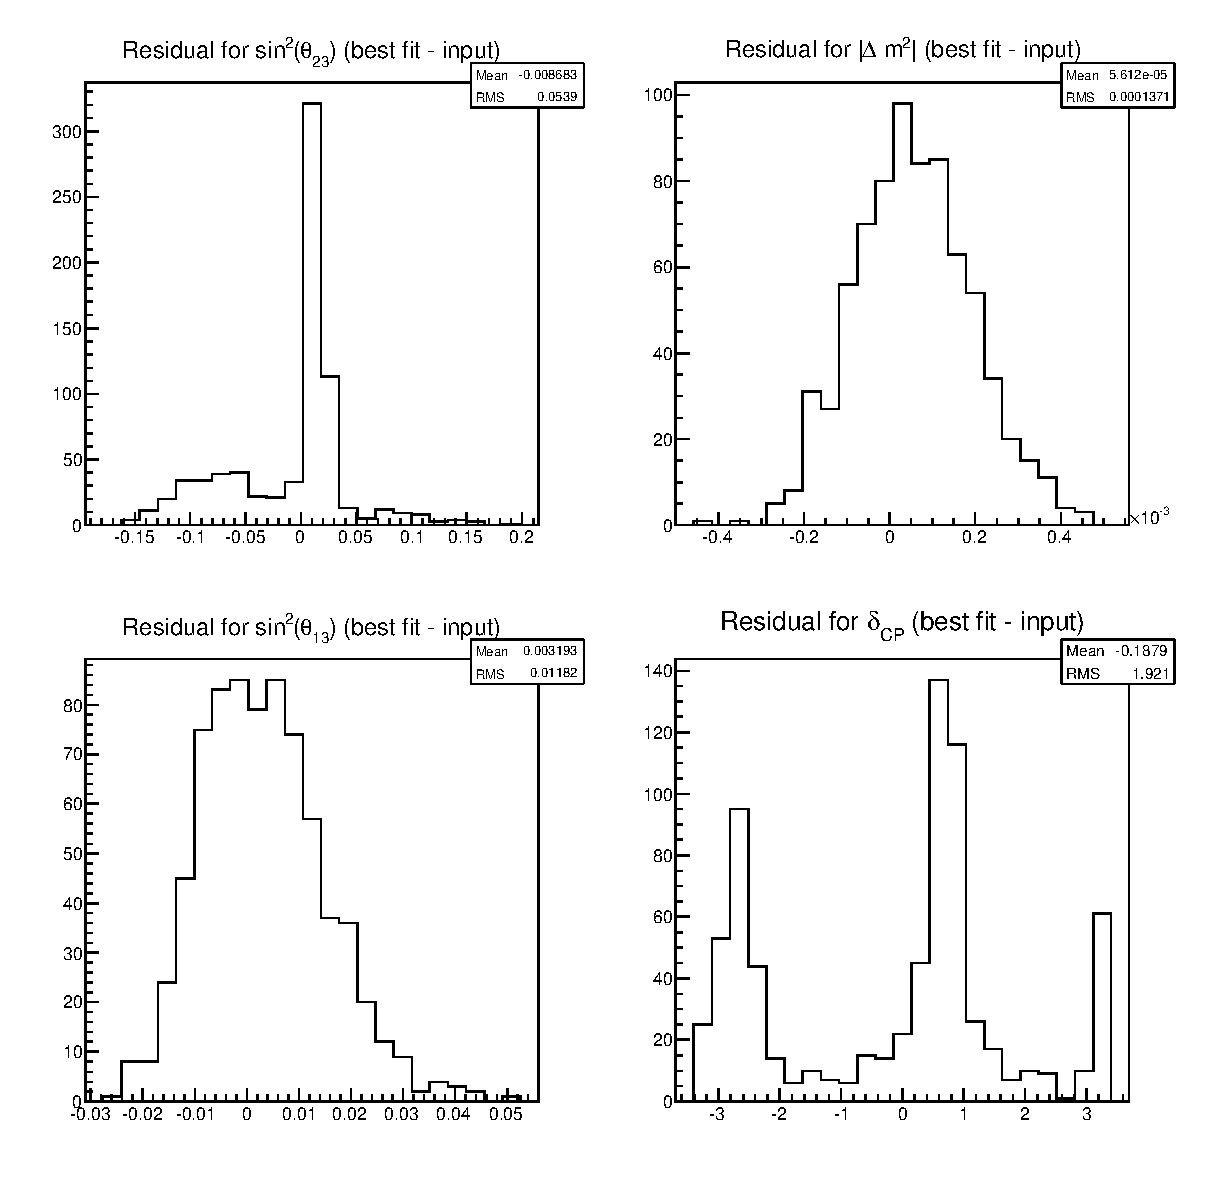
\includegraphics[width=18pc]{images/appendix/fitter_performance/Osc_residuals_nosyst_point7.eps}
\caption{
	Distribution of residuals of the four oscillation parameters in the '4 + 0' fit for oscillation point \# 7. 
 }
\label{fig:residuals_40_point7}
\end{minipage}
\hspace{0.02\linewidth}
\begin{minipage}[t]{0.5\linewidth}
\center
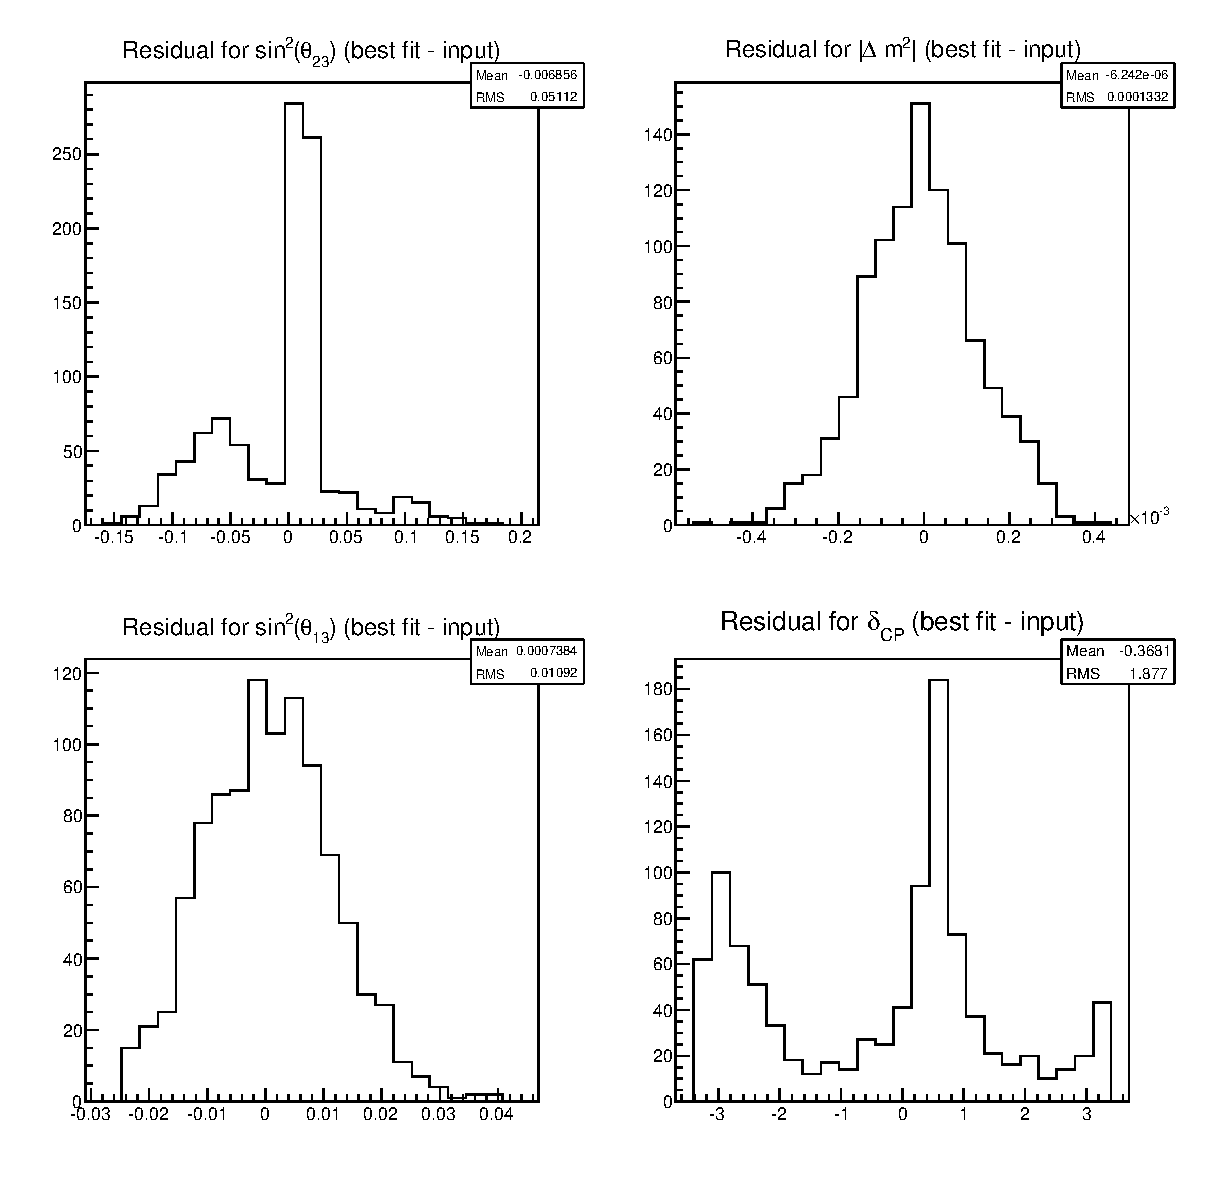
\includegraphics[width=18pc]{images/appendix/fitter_performance/Osc_residuals_nosyst_point8.eps}
\caption{
	Distribution of residuals of the four oscillation parameters in the '4 + 0' fit for oscillation point \# 8. 
 }
 \label{fig:residuals_40_last}
\end{minipage}

\end{figure*}





\begin{figure*}[htbc]
\center
%\begin{minipage}[t]{0.5\linewidth}
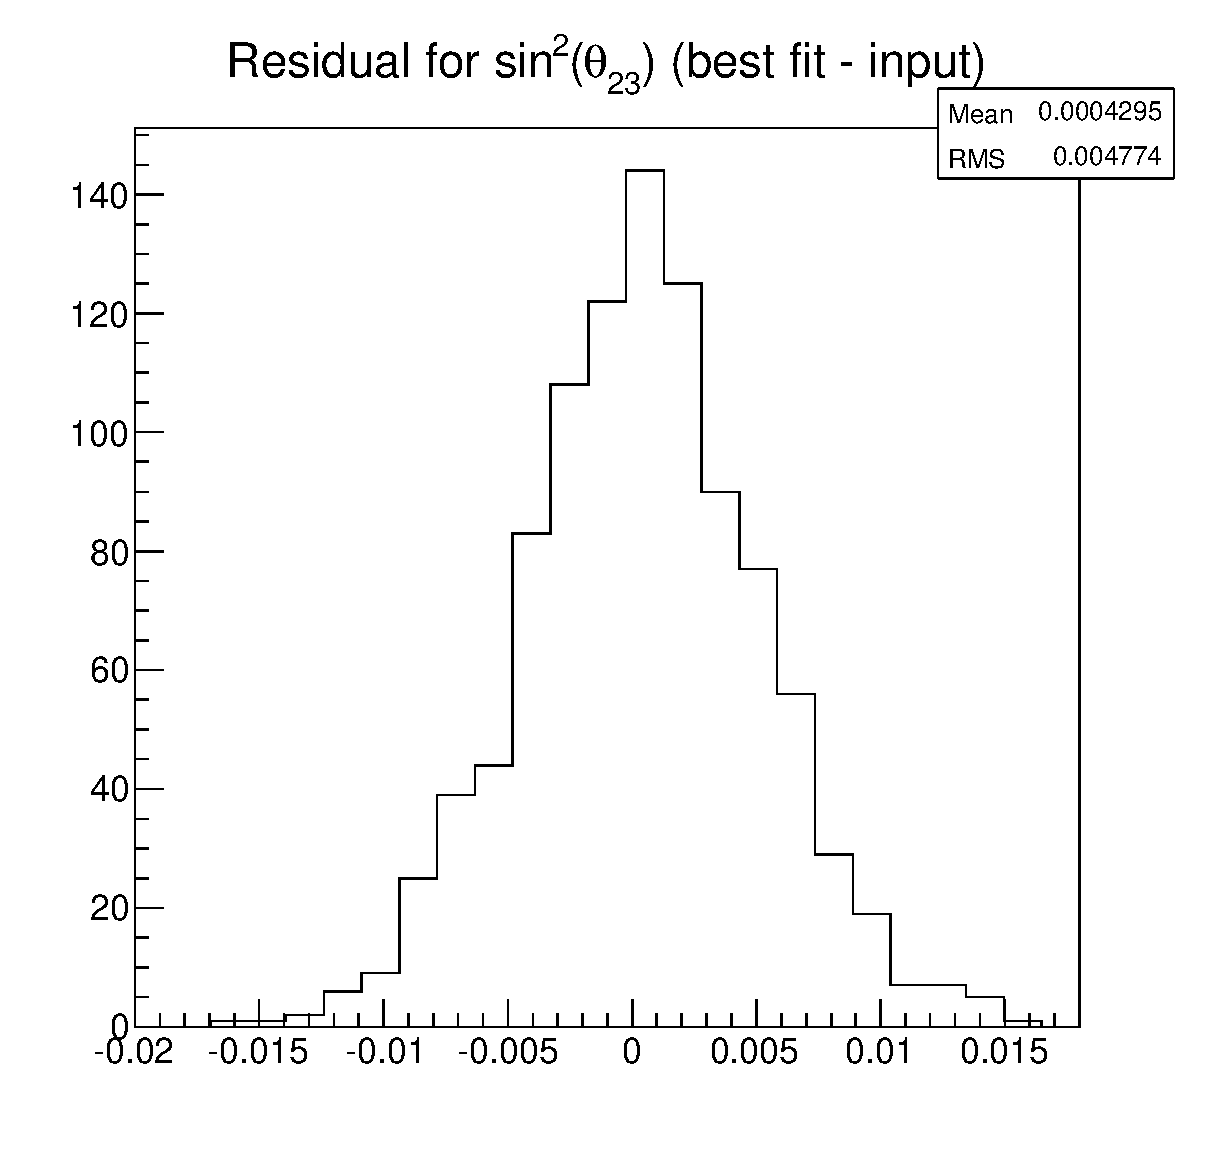
\includegraphics[width=18pc]{images/appendix/fitter_performance/Osc_residuals_nosyst_point1_x100.eps}
\caption{
	Distribution of residuals for $sin^{2}(\theta_{23})$ in the '4 + 0' fit for oscillation point \# 1 with $3.010 \times 10^{22}$ POT. 
 }
\label{fig:residuals_40_point1_x100}
%\end{minipage}
\end{figure*}



\clearpage

\subsection{'4 + 83' fit}

Figs.\ \ref{fig:residuals_483_first} - \ref{fig:residuals_483_last} show the distribution of residuals of the four oscillation parameters 
for each set described in table \ref{tab:osc_points} at $3.010 \times 10^{20}$ POT, with all systematic fluctuations.
As an example, Figs.\ \ref{fig:residuals_483_syst_first} - \ref{fig:residuals_483_syst_last} show the distribution of residuals for each systematic 
parameter for oscillation point \# 0. 
For the rest of oscillation points only summary plots showing the mean and its error ($\frac{RMS}{\sqrt{N}}$)  for all systematic parameters will be presented 
(Figs.\ \ref{fig:systematics_point0} - \ref{fig:systematics_point9})  
The numbering convention for the systematic parameters in those figures can  
be found in table \ref{tab:numbering_syst}. After comparing figures  \ref{fig:residuals_483_first} - \ref{fig:residuals_483_last} 
with  \ref{fig:residuals_40_first} - \ref{fig:residuals_40_last} it can be concluded that fitting all systematics does not change 
the distributions of residuals for the oscillation parameters.
From Figs.\ \ref{fig:systematics_point0} - \ref{fig:systematics_point9} there are three systematics with a "biased" mean of 
the distribution of residuals. The reason for this was found and will be explained now. 
Apart from that there are still no unexpected features.

The three systematics with a "biased" mean of the distribution of residuals are:

\begin{enumerate}
\item{{\bf Spectral function}: The reason for the distribution of residuals for this parameter to be "biased" is the special distribution function used to tweak this systematic parameter, which is uniform from 0 to 1, centered at 0.5, instead of gaussian.		
It was checked that when using a gaussian distribution as for the rest, this "bias" disappeared. However, the use of a uniform function will be kept for this parameter as it was done for the disappearance analysis.
}
\item{{\bf Pi-less delta decay}:The explanation for the "bias" in its distribution of residuals comes from the special response function used for this for this parameter, 
which was only calculated up to $-1\sigma$ and then propagated to $-3\sigma$ with the same value as for $-1\sigma$.
This pathology disappears when constraining this parameter with boundaries $-1\sigma$ to $1\sigma$. 
}
\item{{\bf $1R_{\mu}$ NC efficiency}:The reason for this parameter to have a "biased" distribution of residuals comes from the low statistics at current POT.
When Poisson fluctuations are made of the bin contents of the $E_{reco}$ distributions, a downward fluctuation is more likely than an upward fluctuation (see replies to comments and revision history for TN141).
Adding the fact that the NC modes are distributed around the oscillation maximum, the (most likely) downwards Poisson fluctuations translate into a (most likely) negative value of the NC efficiency, explaining a "bias" to negative values for this parameter.
It was checked that the "bias" in the distribution depends on the true input value of $sin^{2}\theta_{23}$, disappearing when $sin^{2}\theta_{23}$ is far away from 0.5; and also that it decreases as well when increasing the POT. 
}
\end{enumerate}


\begin{table}[htbp]
\center
\begin{tabular}{|p{3cm}|p{7cm}|}
\hline 
\# & Systematic \\
\hline 
0 -24 & BANFF $\nu_{\mu}$, $\bar{\nu_{\mu}}$, $\nu_{e}$ and $\bar{\nu_{e}}$ flux bins \\
25  & BANFF CCQE axial mass \\
26 & BANFF resonance-production axial mass \\
27-29 & CCQE normalization \\
30-31 & CC 1$\pi$ normalization \\
32 & NC1$\pi0$ \\
\hline
33 & Fermi momentum \\
34 & Nuclear modeling (Spectral function) \\
35 & Binding energy \\
36 & Shape of $\pi$ momentum distribution (W shape) \\
37 & CC other shape\\
38 & $\pi$-less $\Delta$ decay\\
39 & CC coherent normalization \\
40 & NC 1$\pi^{\pm}$ normalization \\
41 & NC coherent normalization \\
42 & NC other normalizarion \\
43 & $\sigma_{\nu_{e}}/\sigma_{\nu_{\mu}}$ ratio \\
44 & $\sigma_{\bar{\nu}}/\sigma_{\nu}$ ratio \\
\hline
45 & Reconstructed energy scale \\
46-48 & $\nu_{\mu}$, $\bar{\nu_{\mu}}$ CCQE ring counting efficiency \\
49 & $\nu_{\mu}$, $\bar{\nu_{\mu}}$ CCQE other efficiency \\
50 & $\nu_{\mu}$, $\bar{\nu_{\mu}}$ CCnonQE efficiency \\
51 & NC efficiency \\
52 & $\nu_{e}$, $\bar{\nu_{e}}$ CC efficiency \\
53-55 & 1$R_{e}$ osc. $\nu_{e}$ CC efficiency \\
56-58 & 1$R_{e}$ $\nu_{\mu}$, $\bar{\nu_{\mu}}$ CC efficiency \\
59-61 & 1$R_{e}$ $\nu_{e}$, $\bar{\nu_{e}}$ CC efficiency \\
62-64 & 1$R_{e}$ NC efficiency \\
\hline
65-67 & 1$R_{\mu}$  FSI: $\nu_{\mu}$, $\bar{\nu_{\mu}}$ CCQE  \\
68 & $R_{\mu}$  FSI: $\nu_{\mu}$, $\bar{\nu_{\mu}}$ CCnonQE efficiency \\
69 & $R_{\mu}$  FSI: $\nu_{e}$, $\bar{\nu_{e}}$ CC\\
70 & $R_{\mu}$  FSI: NC  \\
\hline
71-73 & 1$R_{e}$ FS: osc. $\nu_{e}$ CC  \\
74-76 & 1$R_{e}$ FSI: $\nu_{\mu}$, $\bar{\nu_{\mu}}$ CC  \\
77-79 & 1$R_{e}$ FSI: $\nu_{e}$, $\bar{\nu_{e}}$ CC  \\
80-82 & 1$R_{e}$ FSI: NC  \\
\hline
\end{tabular}\\[2pt]
\caption{
  The numbering of systematic parameters for figures  \ref{fig:systematics_point0} - \ref{fig:systematics_point9} 
}
\label{tab:numbering_syst}
\end{table}



\clearpage



\begin{figure*}[htb]
\begin{minipage}[t]{0.5\linewidth}
\center
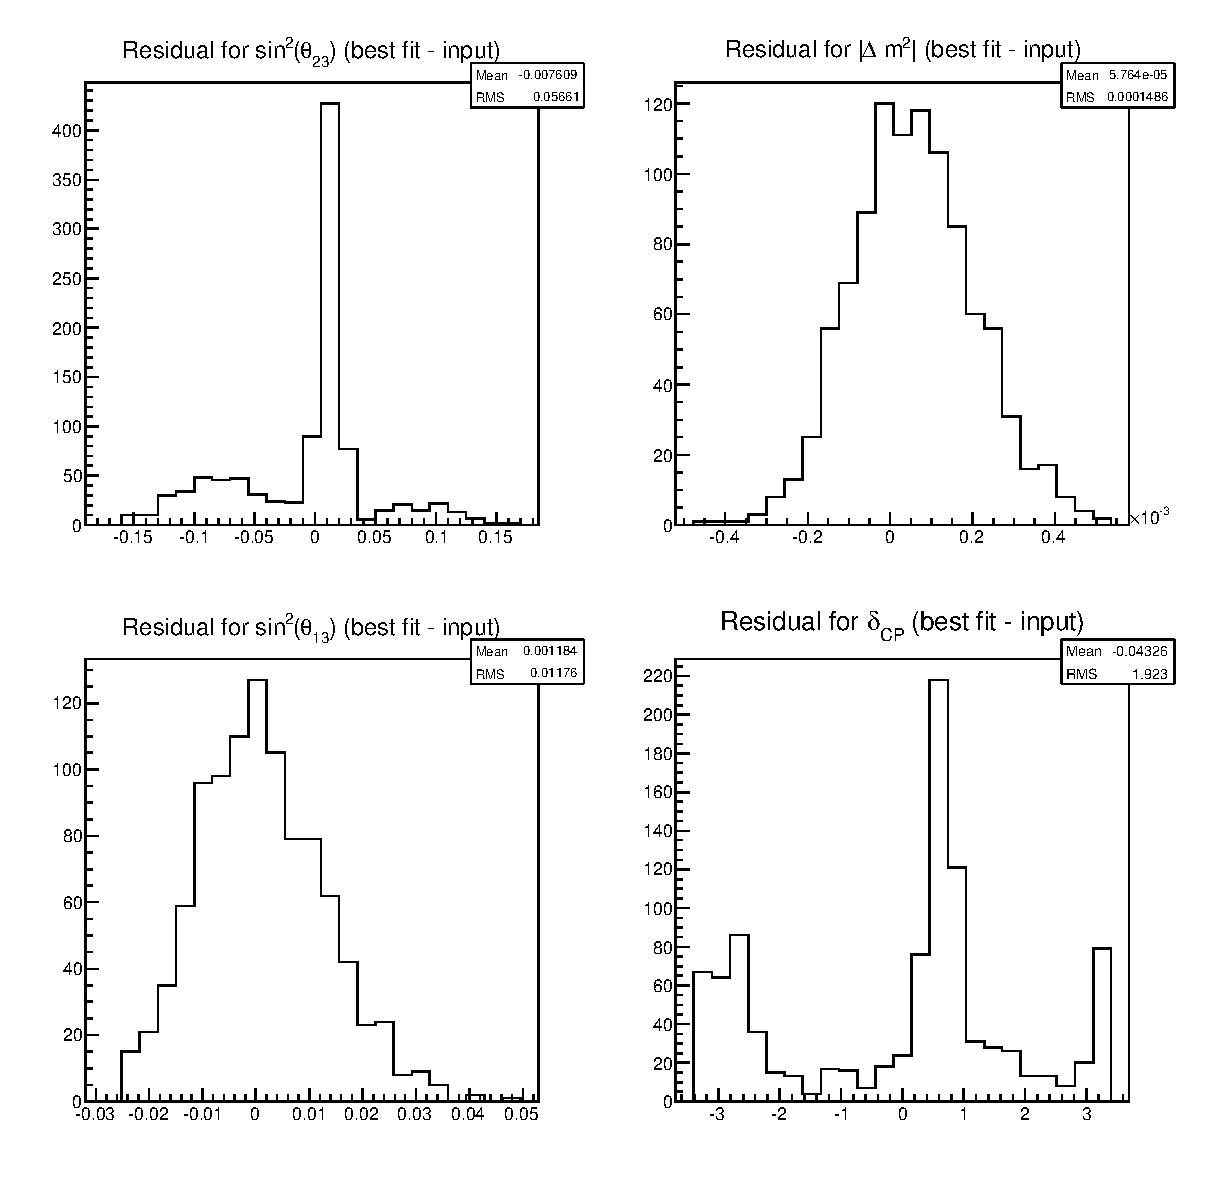
\includegraphics[width=18pc]{images/appendix/fitter_performance/Osc_residuals_joint_syst_point0.eps}
\caption{
	Distribution of residuals of the four oscillation parameters in the '4 + 83' fit for oscillation point \# 0. 
 }
\label{fig:residuals_483_first}
\end{minipage}
\hspace{0.02\linewidth}
\begin{minipage}[t]{0.5\linewidth}
\center
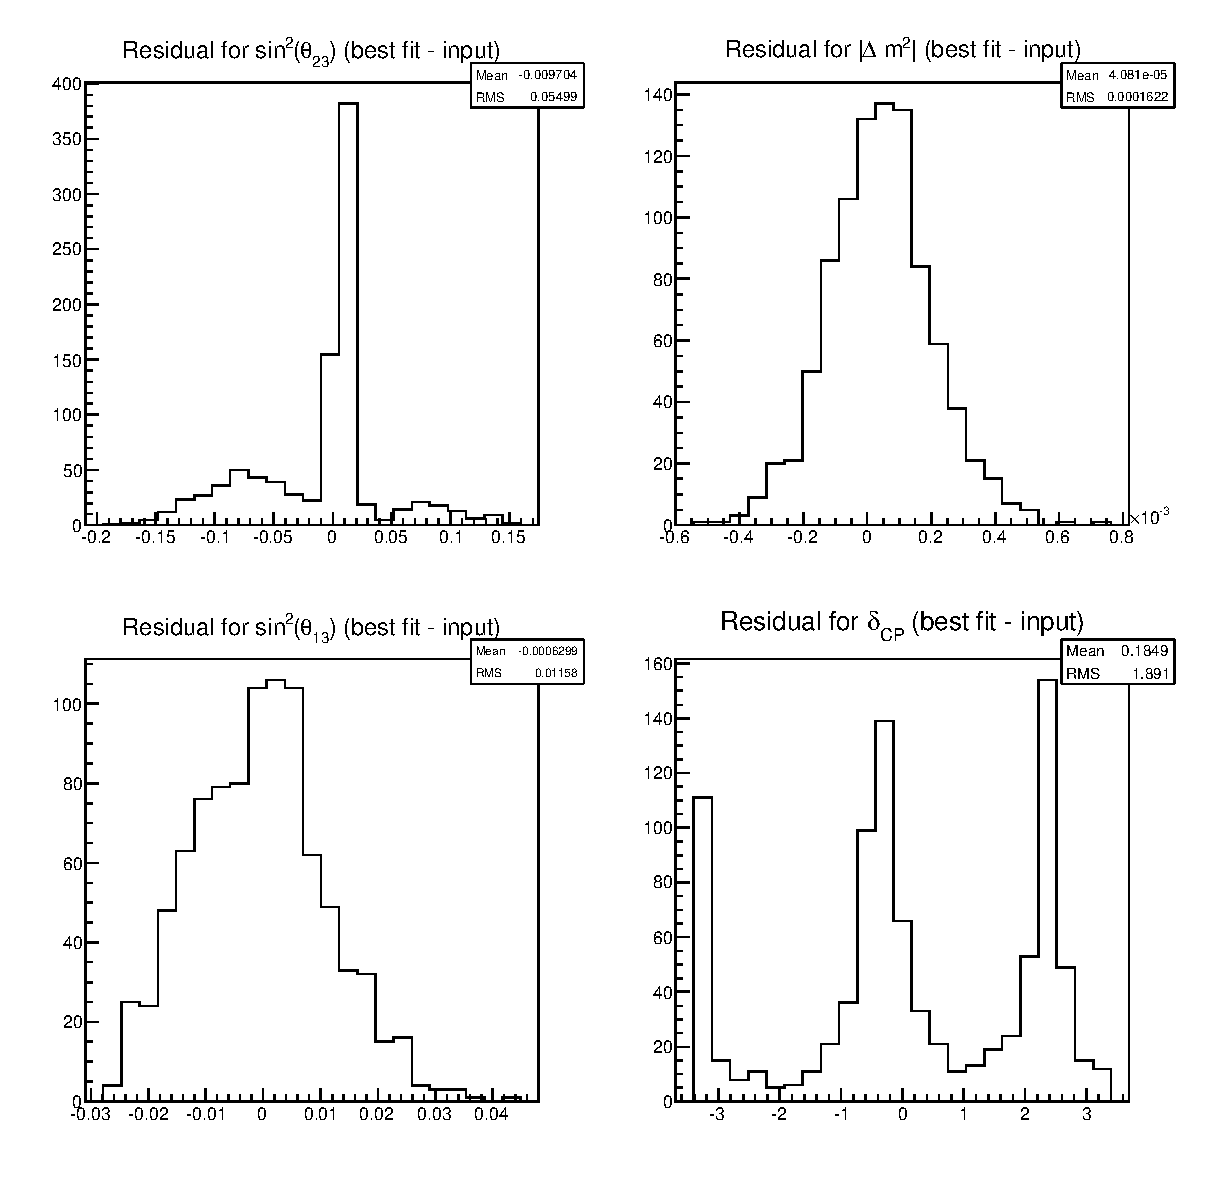
\includegraphics[width=18pc]{images/appendix/fitter_performance/Osc_residuals_joint_syst_point9.eps}
\caption{
	Distribution of residuals of the four oscillation parameters in the '4 + 83' fit for oscillation point \# 9. 
 }
\end{minipage}

\end{figure*}


\begin{figure*}[htb]
\begin{minipage}[t]{0.5\linewidth}
\center
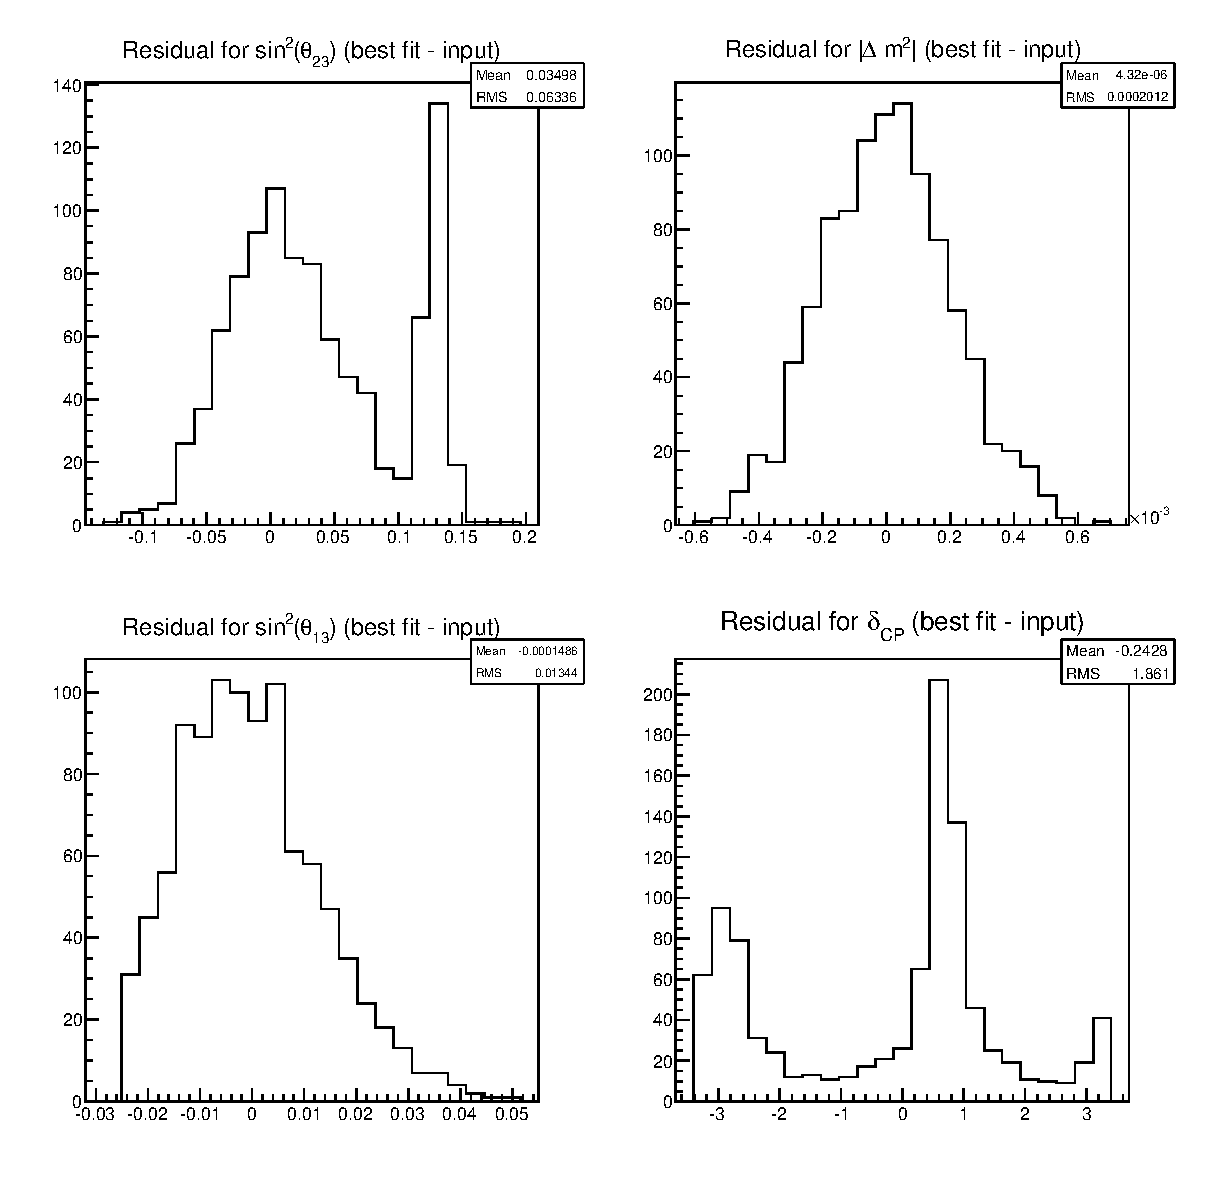
\includegraphics[width=18pc]{images/appendix/fitter_performance/Osc_residuals_joint_syst_point1.eps}
\caption{
	Distribution of residuals of the four oscillation parameters in the '4 + 83' fit for oscillation point \# 1. 
 }
\label{fig:residuals_483_point1}
\end{minipage}
\hspace{0.02\linewidth}
\begin{minipage}[t]{0.5\linewidth}
\center
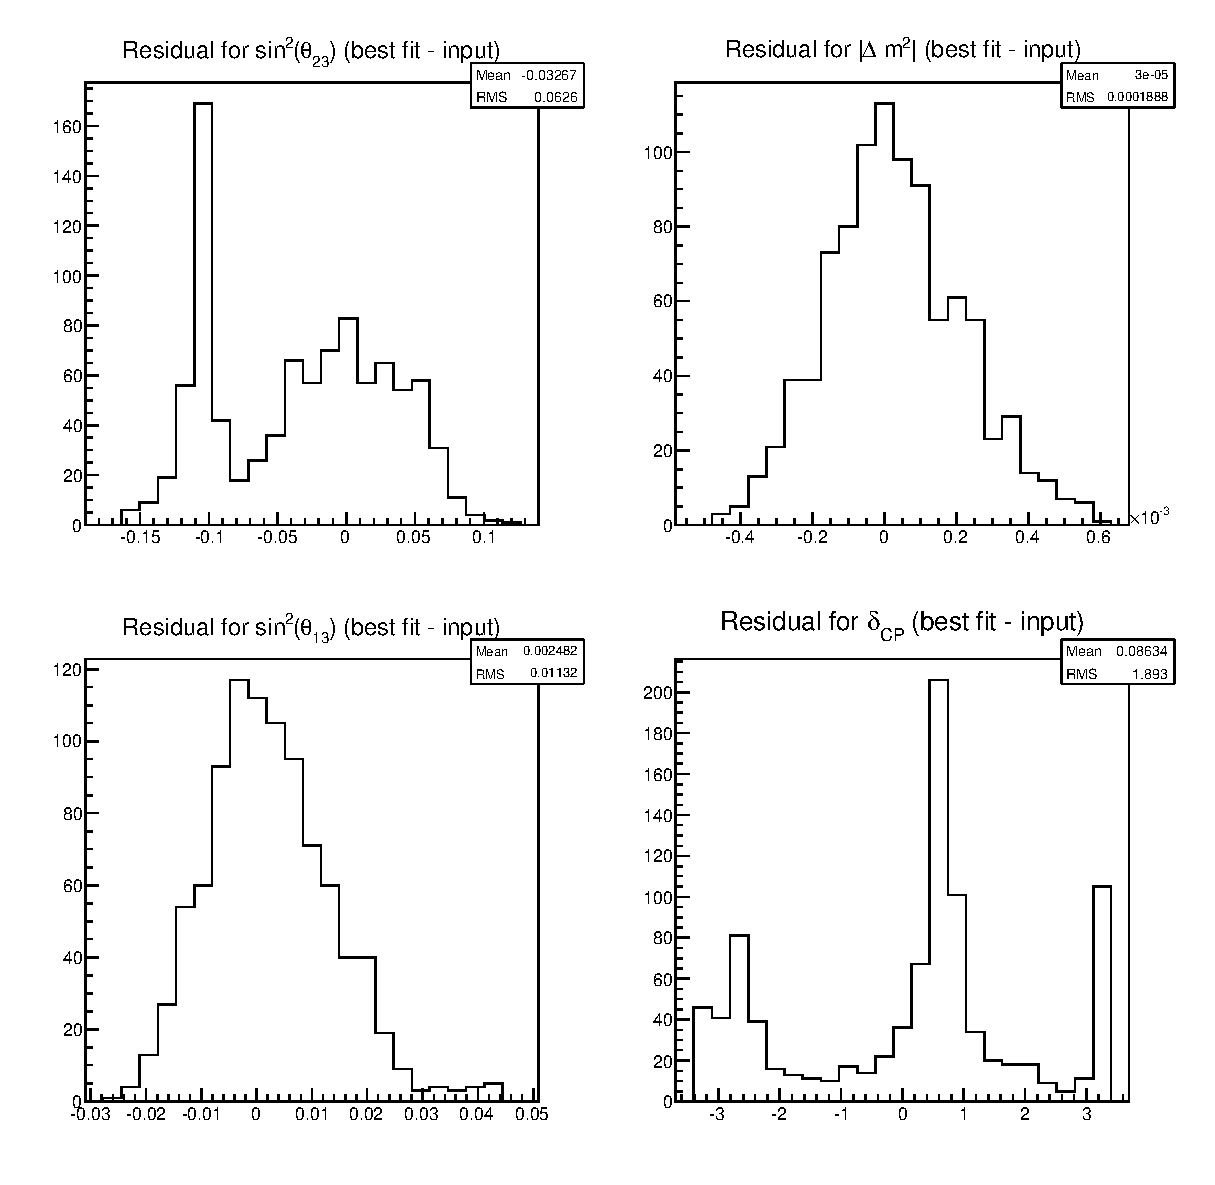
\includegraphics[width=18pc]{images/appendix/fitter_performance/Osc_residuals_joint_syst_point2.eps}
\caption{
	Distribution of residuals of the four oscillation parameters in the '4 + 83' fit for oscillation point \# 2. 
 }
\end{minipage}

\end{figure*}

\clearpage

\begin{figure*}[htb]
\begin{minipage}[t]{0.5\linewidth}
\center
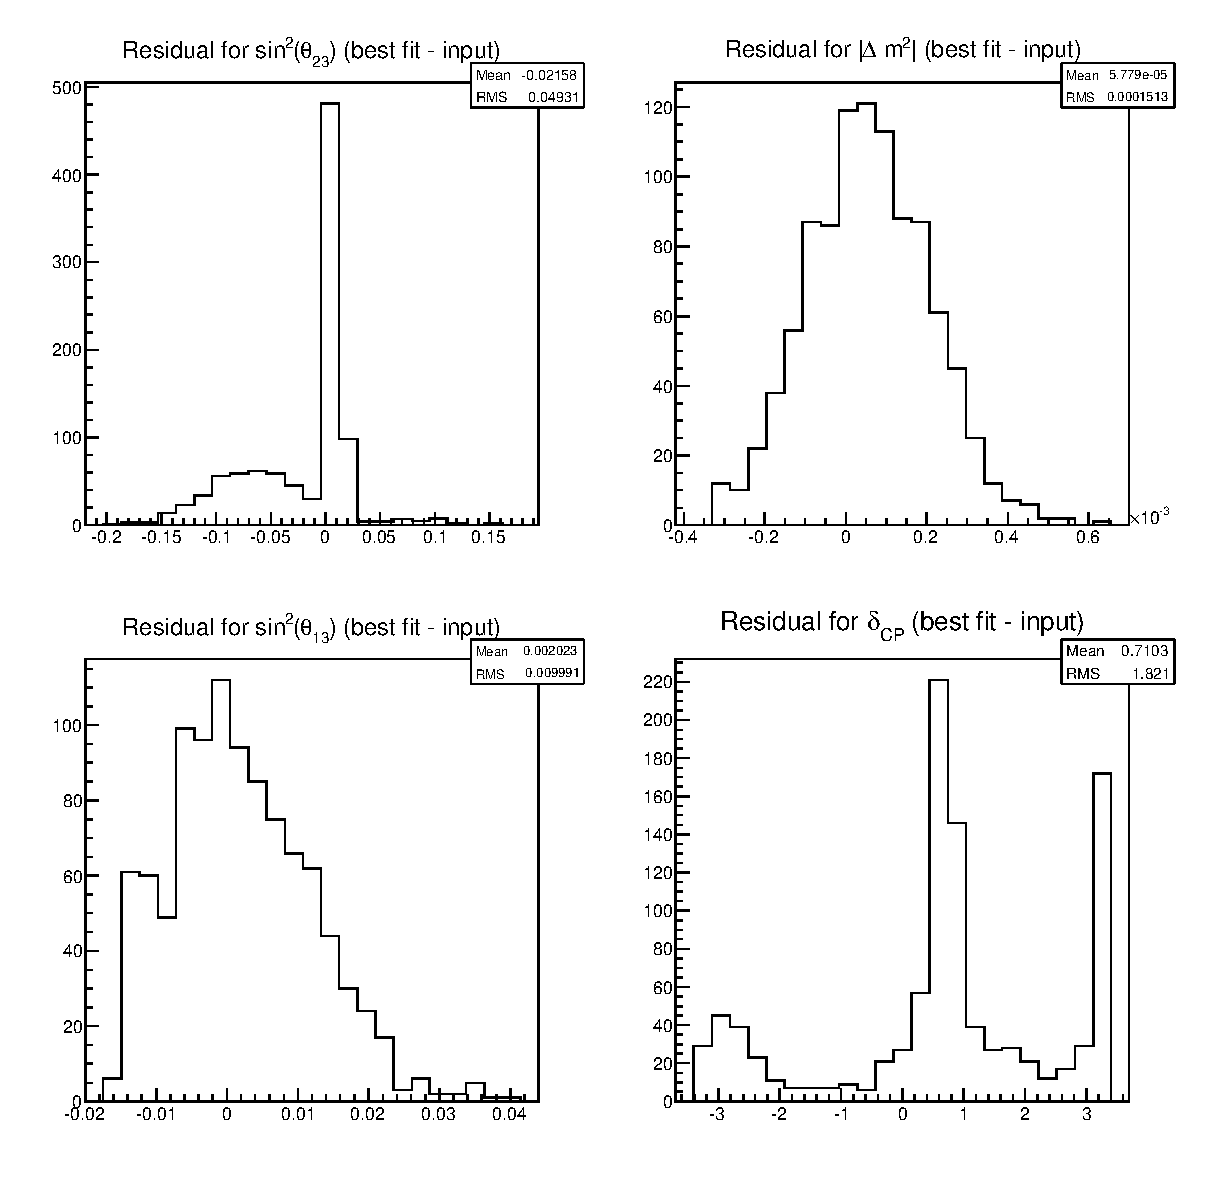
\includegraphics[width=18pc]{images/appendix/fitter_performance/Osc_residuals_joint_syst_point3.eps}
\caption{
	Distribution of residuals of the four oscillation parameters in the '4 + 83' fit for oscillation point \# 3. 
 }
\label{fig:residuals_483_point3}
\end{minipage}
\hspace{0.02\linewidth}
\begin{minipage}[t]{0.5\linewidth}
\center
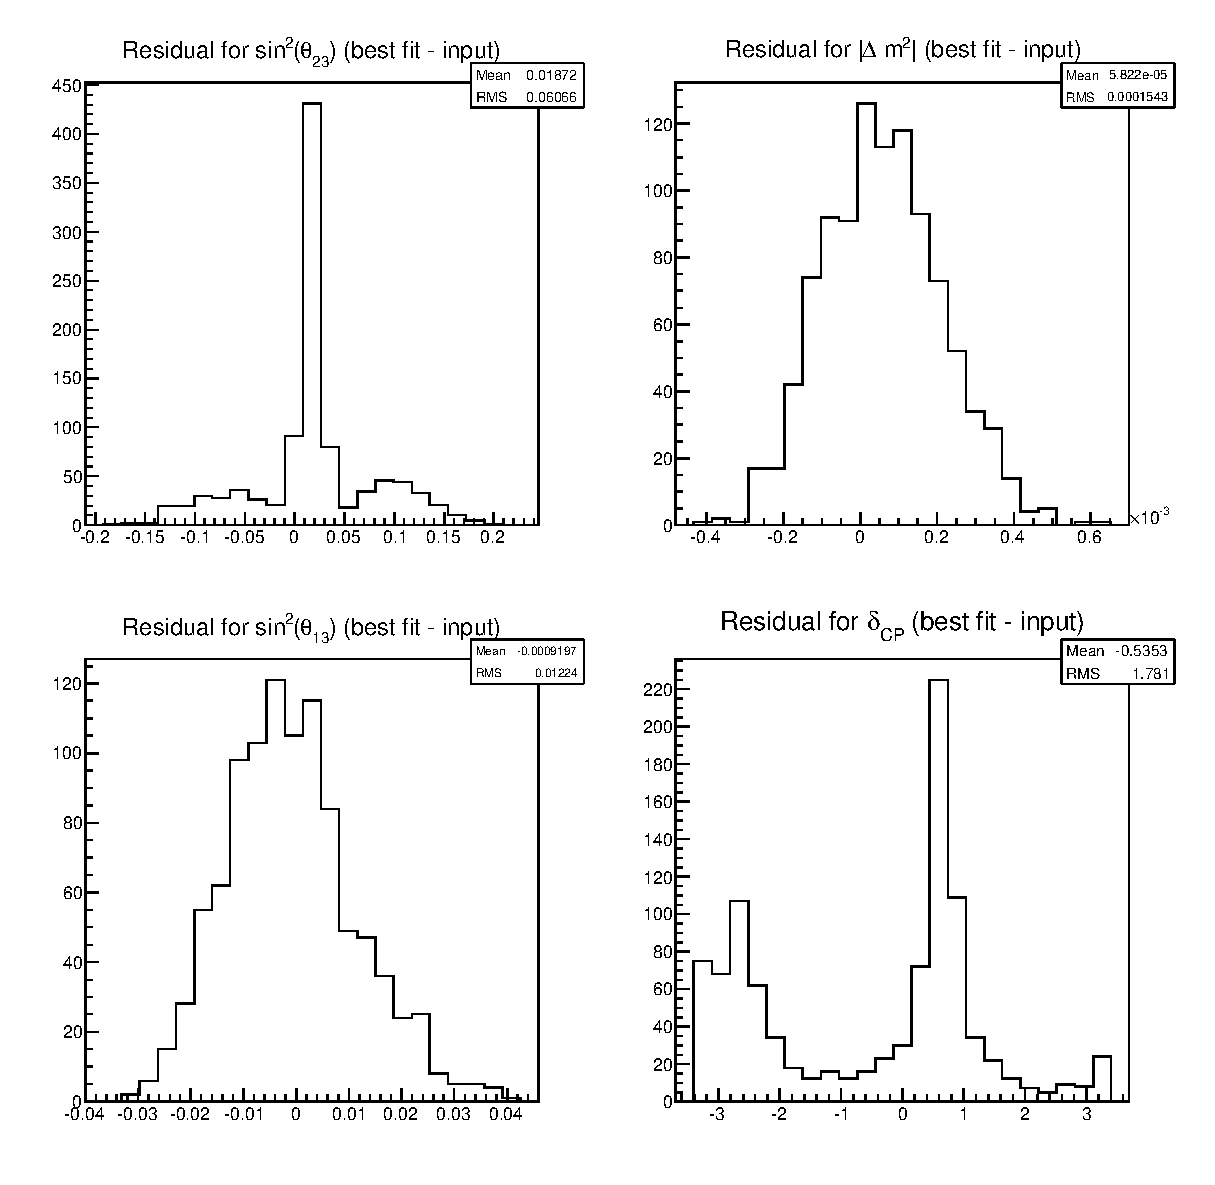
\includegraphics[width=18pc]{images/appendix/fitter_performance/Osc_residuals_joint_syst_point4.eps}
\caption{
	Distribution of residuals of the four oscillation parameters in the '4 + 83' fit for oscillation point \# 4. 
 }
\end{minipage}

\end{figure*}


\begin{figure*}[htb]
\begin{minipage}[t]{0.5\linewidth}
\center
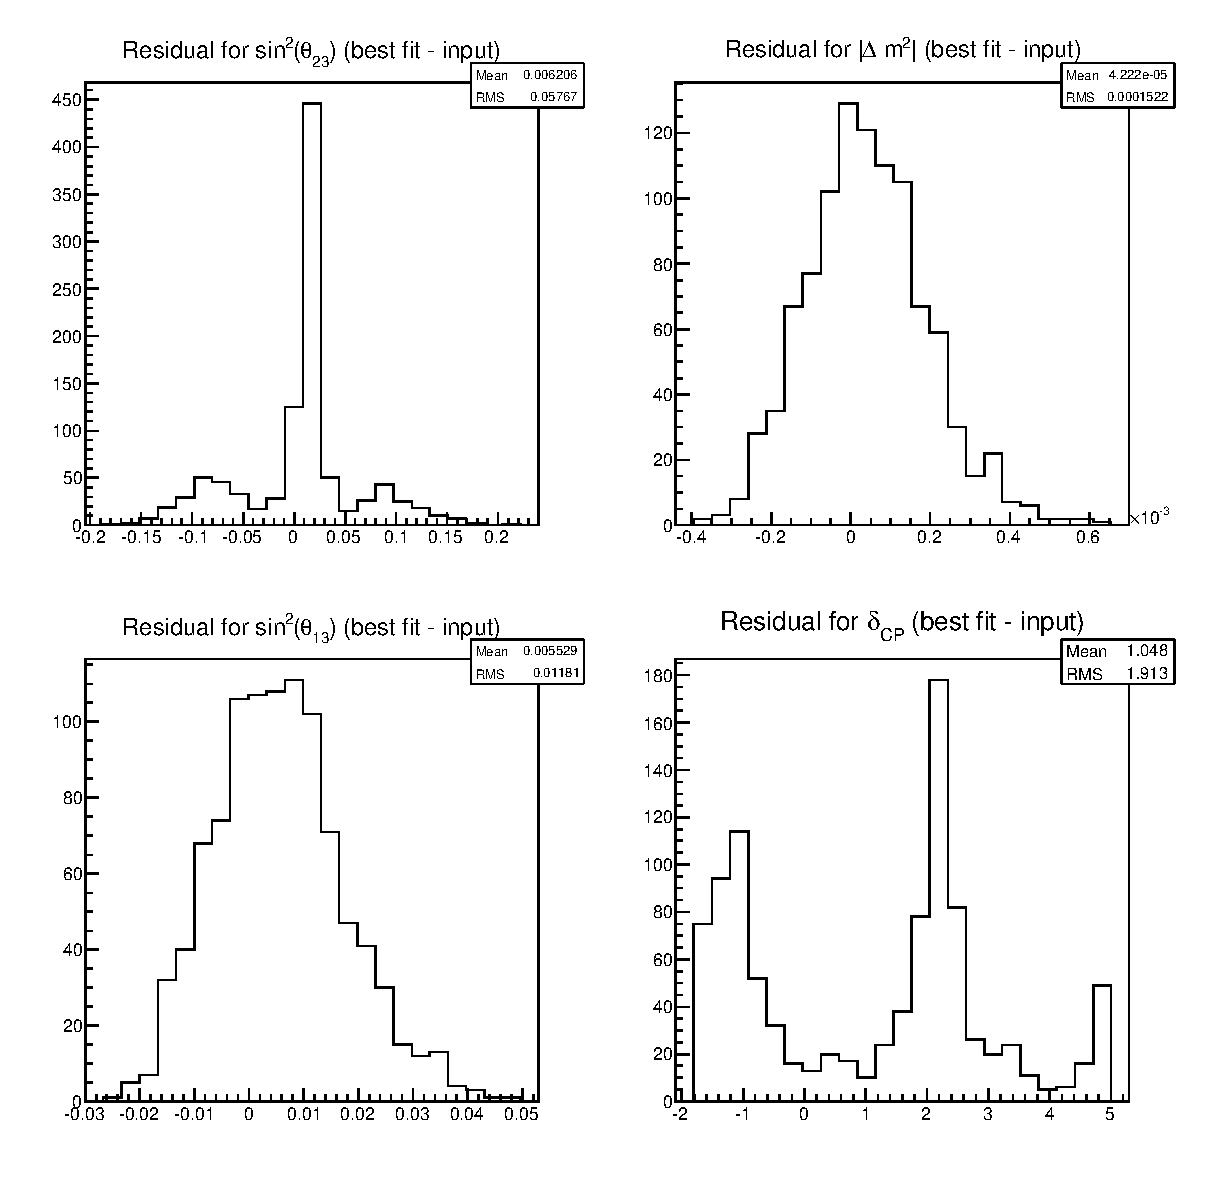
\includegraphics[width=18pc]{images/appendix/fitter_performance/Osc_residuals_joint_syst_point5.eps}
\caption{
	Distribution of residuals of the four oscillation parameters in the '4 + 83' fit for oscillation point \# 5. 
 }
\label{fig:residuals_483_point5}
\end{minipage}
\hspace{0.02\linewidth}
\begin{minipage}[t]{0.5\linewidth}
\center
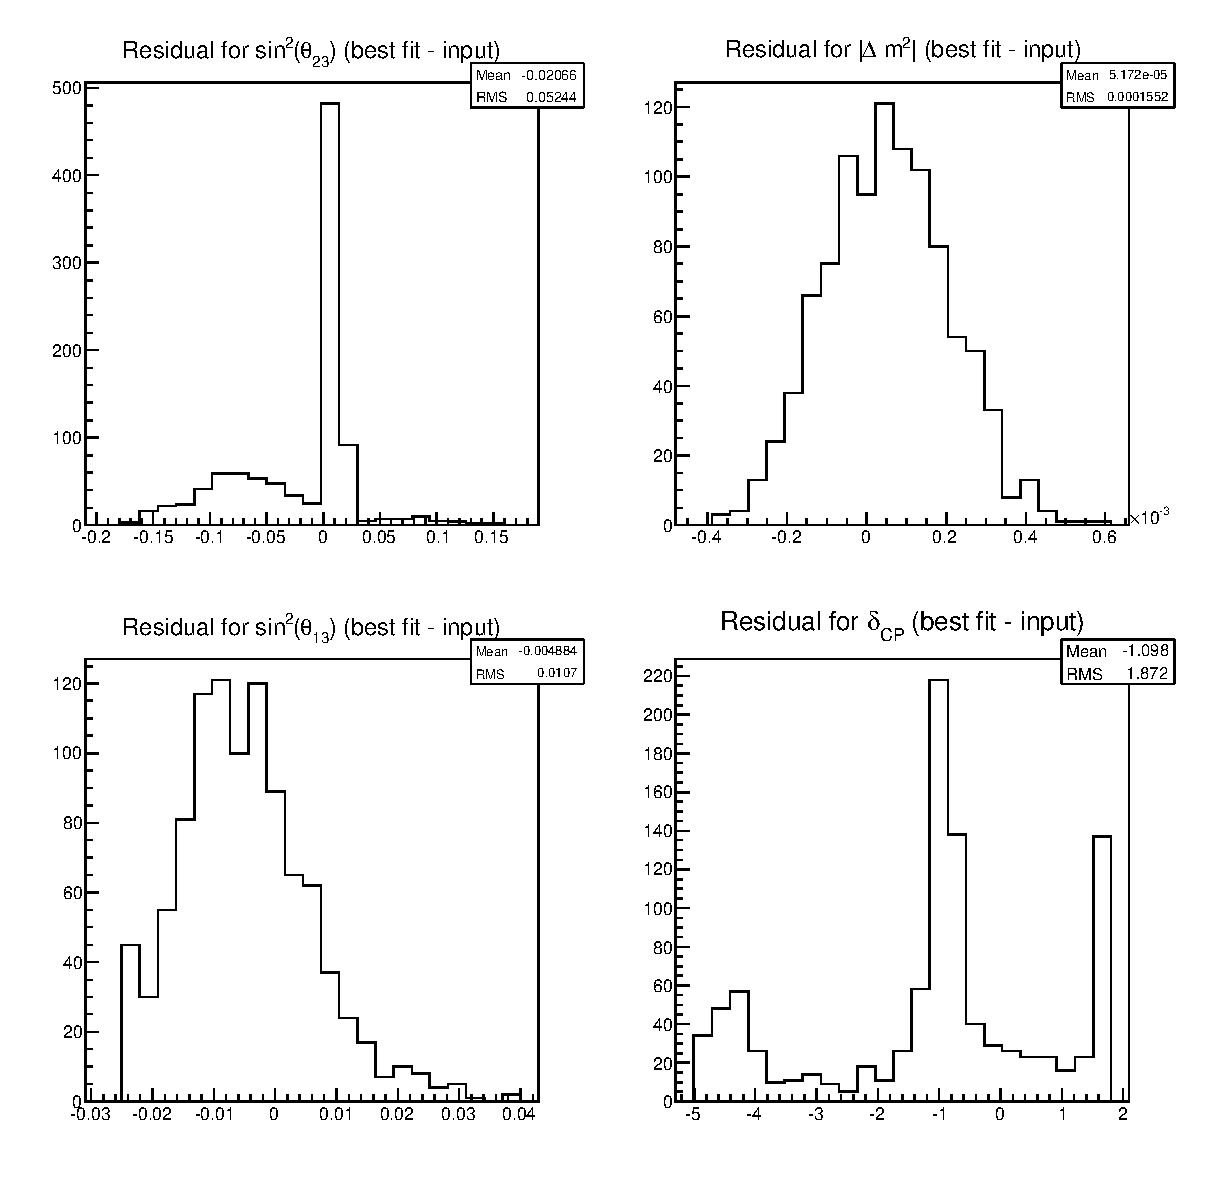
\includegraphics[width=18pc]{images/appendix/fitter_performance/Osc_residuals_joint_syst_point6.eps}
\caption{
	Distribution of residuals of the four oscillation parameters in the '4 + 83' fit for oscillation point \# 6. 
 }
\end{minipage}

\end{figure*}

\clearpage

\begin{figure*}[htb]
\begin{minipage}[t]{0.5\linewidth}
\center
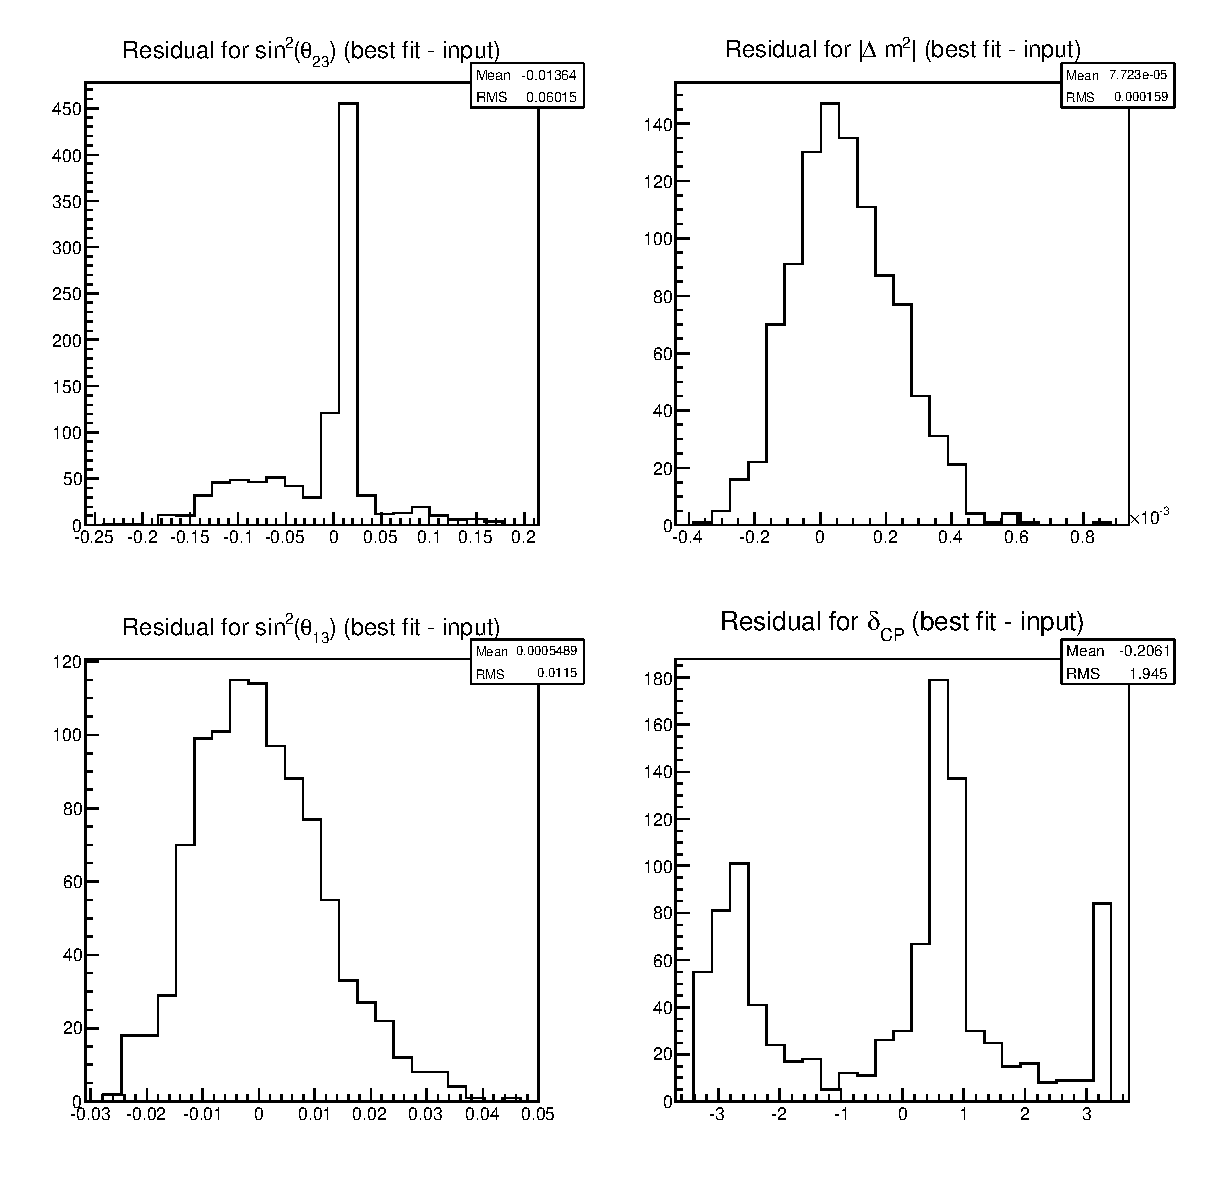
\includegraphics[width=18pc]{images/appendix/fitter_performance/Osc_residuals_joint_syst_point7.eps}
\caption{
	Distribution of residuals of the four oscillation parameters in the '4 + 83' fit for oscillation point \# 7. 
 }
\label{fig:residuals_483_point7}
\end{minipage}
\hspace{0.02\linewidth}
\begin{minipage}[t]{0.5\linewidth}
\center
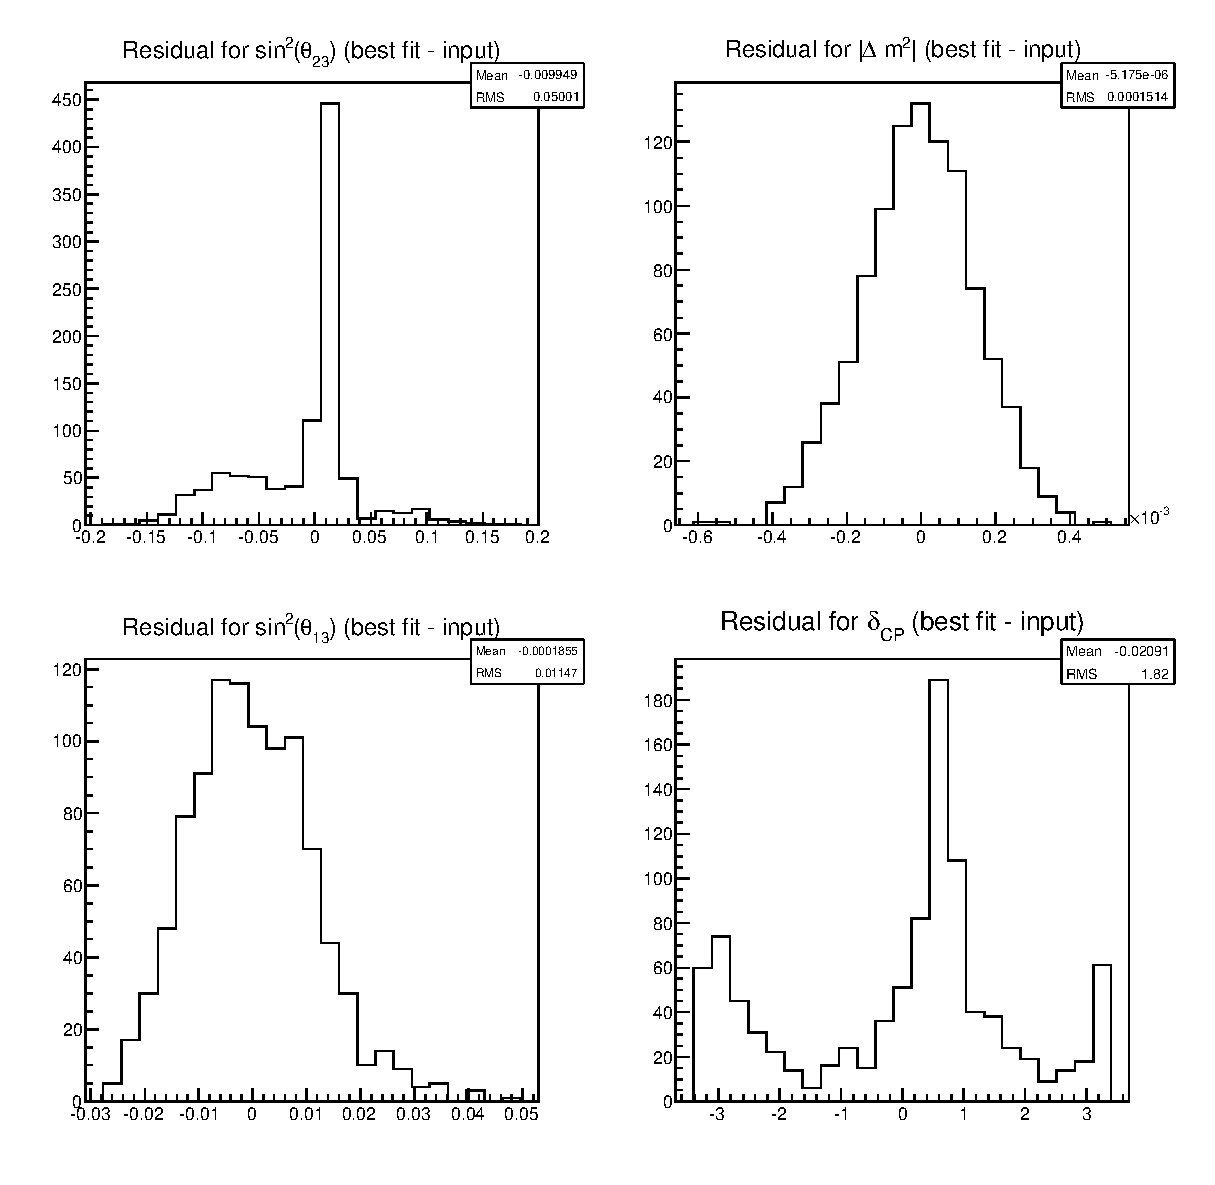
\includegraphics[width=18pc]{images/appendix/fitter_performance/Osc_residuals_joint_syst_point8.eps}
\caption{
	Distribution of residuals of the four oscillation parameters in the '4 + 83' fit for oscillation point \# 8. 
 }
 \label{fig:residuals_483_last}
\end{minipage}

\end{figure*}

\clearpage

%%%% SYSTEMATICS %%%

\begin{figure*}[htbc]	
\center
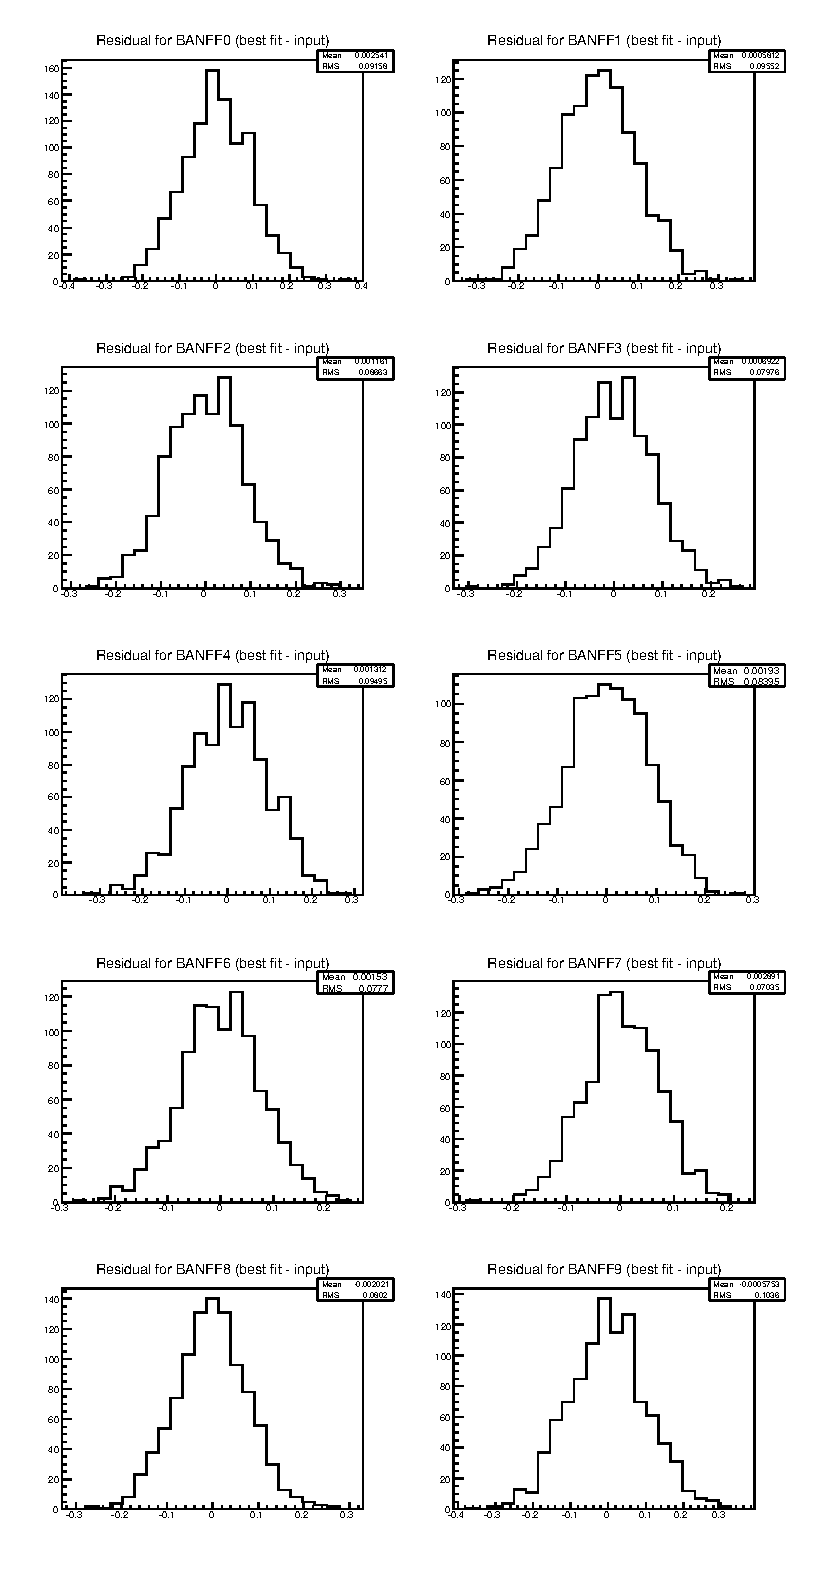
\includegraphics[width=25pc]{images/appendix/fitter_performance/Syst1_residuals_joint_syst_point0.eps}
\caption{
	Distribution of residuals of the BANFF (0-9) systematic parameters in the '4 + 83' fit for oscillation point \# 0. 
 }
\label{fig:residuals_483_syst_first}
\end{figure*}


\begin{figure*}[htbc]	
\center
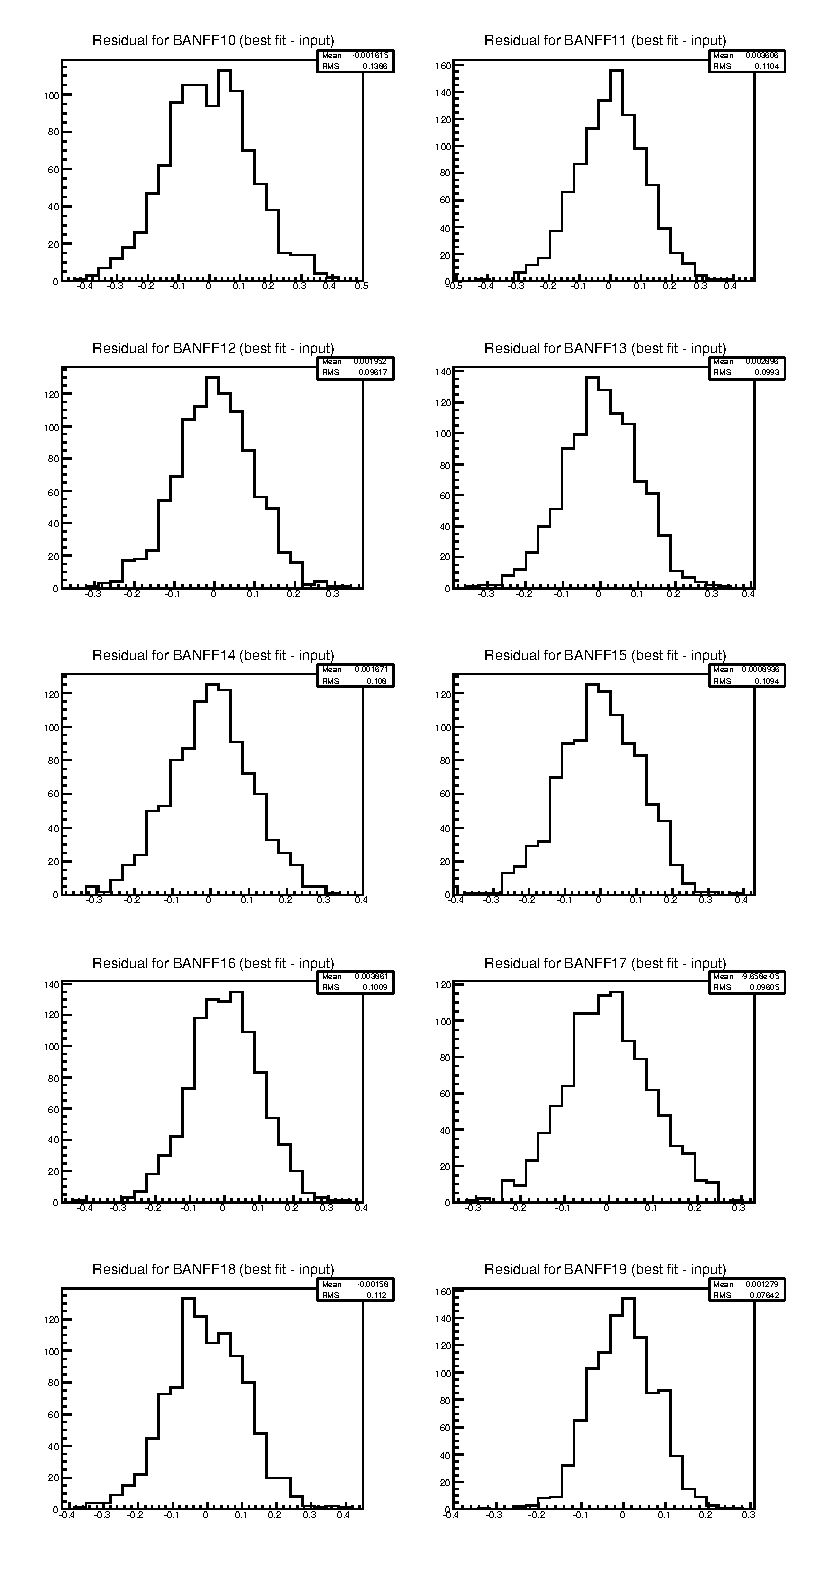
\includegraphics[width=25pc]{images/appendix/fitter_performance/Syst2_residuals_joint_syst_point0.eps}
\caption{
	Distribution of residuals of the BANFF (10-19) systematic parameters in the '4 + 83' fit for oscillation point \# 0. 
 }
\end{figure*}

\begin{figure*}[htbc]	
\center
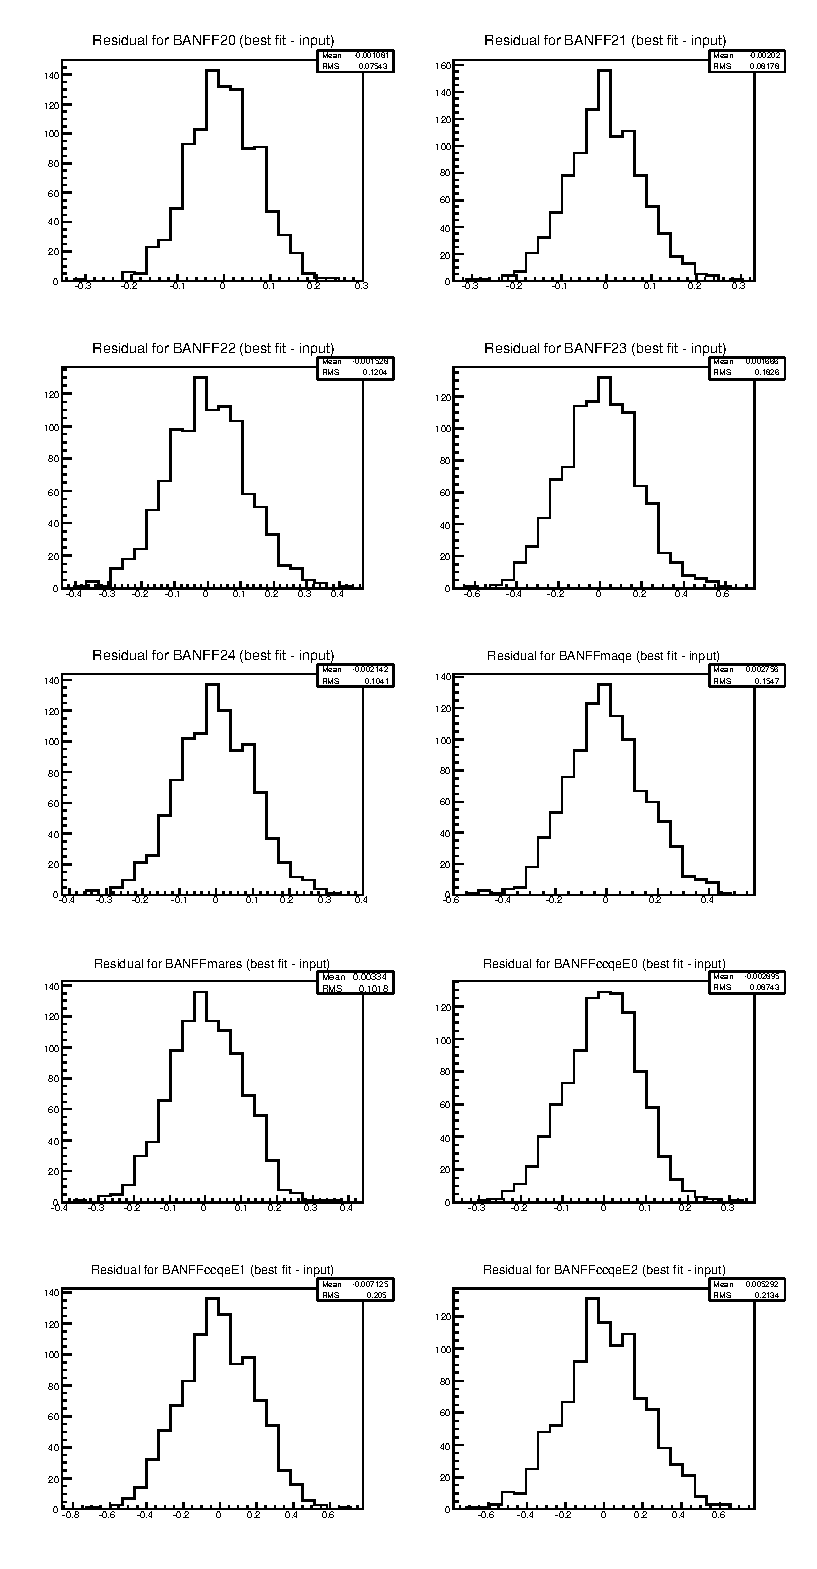
\includegraphics[width=25pc]{images/appendix/fitter_performance/Syst3_residuals_joint_syst_point0.eps}
\caption{
	Distribution of residuals of the  BANFF (20-29) systematic parameters in the '4 + 83' fit for oscillation point \# 0. 
 }
\end{figure*}

\begin{figure*}[htbc]	
\center
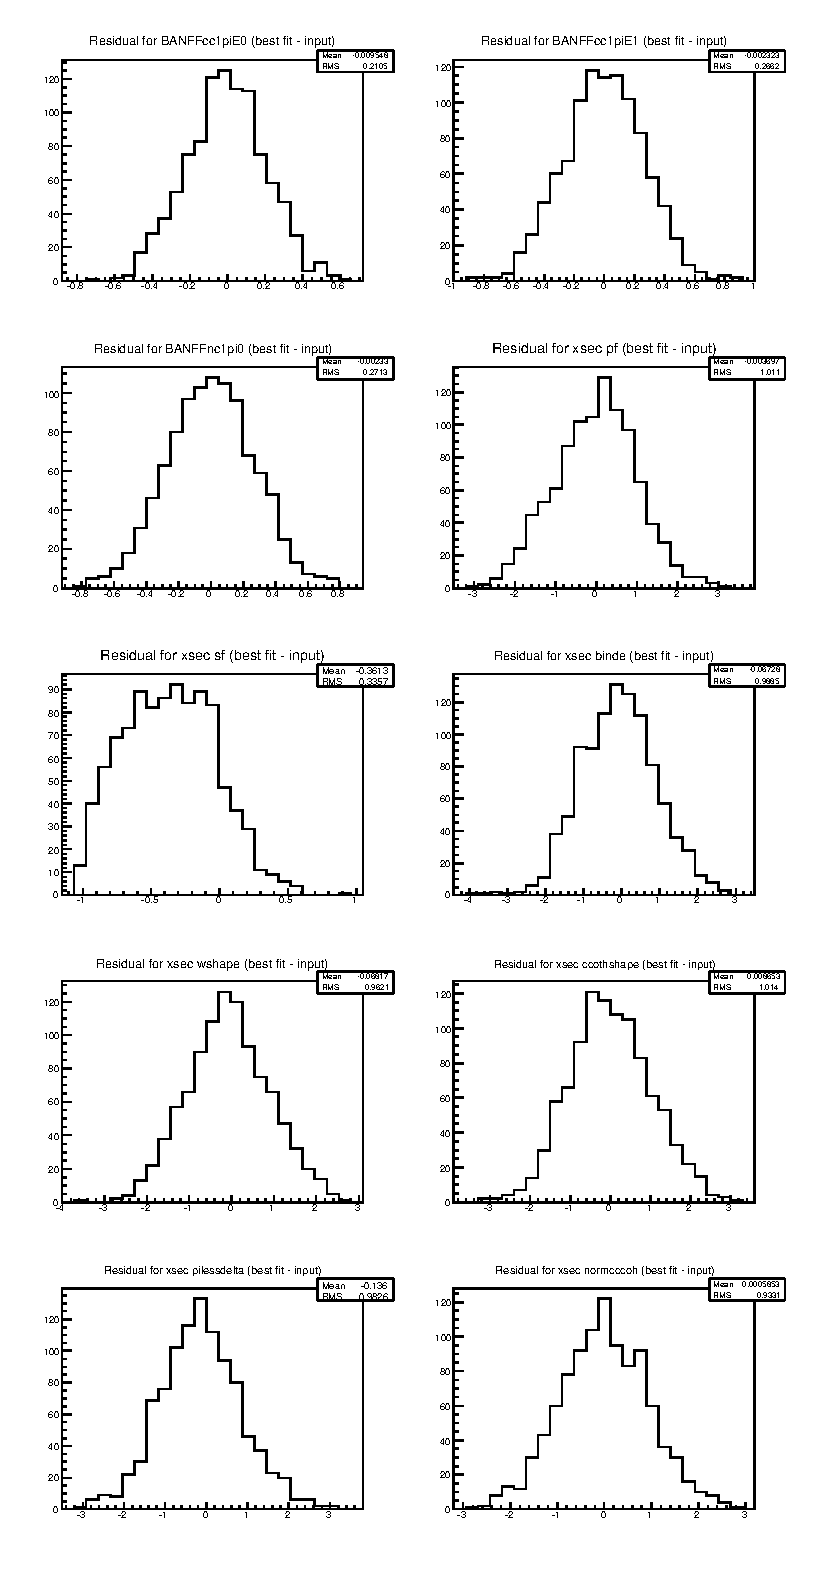
\includegraphics[width=25pc]{images/appendix/fitter_performance/Syst4_residuals_joint_syst_point0.eps}
\caption{
	Distribution of residuals of the BANFF (30-32) and uncorrelated cross sections (I) systematic parameters in the '4 + 83' fit for oscillation point \# 0. 
 }
\end{figure*}

\begin{figure*}[htbc]	
\center
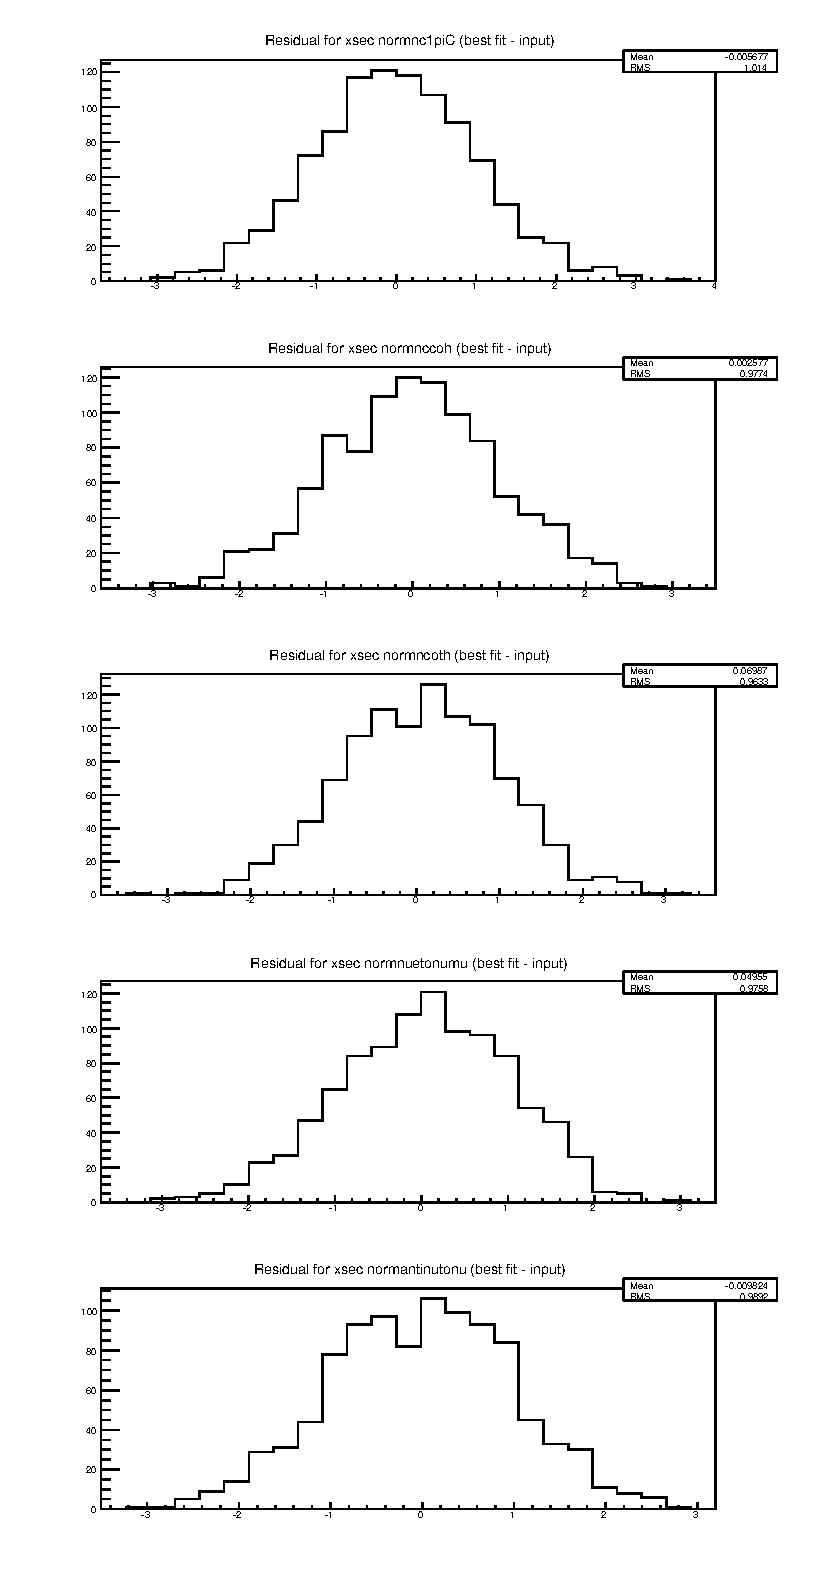
\includegraphics[width=20pc]{images/appendix/fitter_performance/Syst5_residuals_joint_syst_point0.eps}
\caption{
	Distribution of residuals of uncorrelated cross sections (II) systematic parameters in the '4 + 83' fit for oscillation point \# 0. 
 }
\end{figure*}


\begin{figure*}[htbc]	
\center
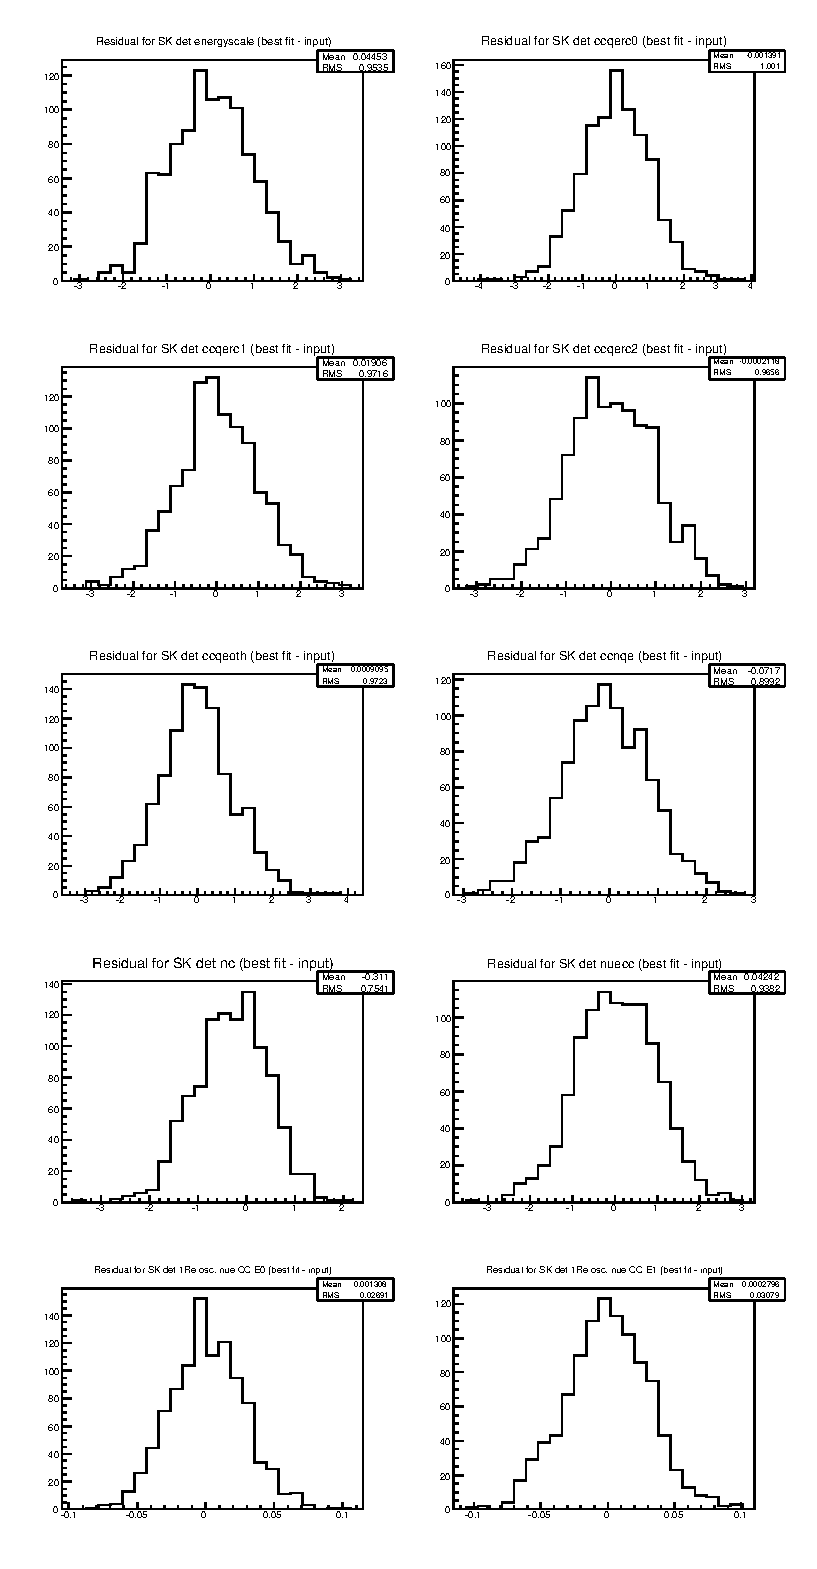
\includegraphics[width=25pc]{images/appendix/fitter_performance/Syst6_residuals_joint_syst_point0.eps}
\caption{
	Distribution of residuals of SK detector (I) systematic parameters in the '4 + 83' fit for oscillation point \# 0. 
 }
\end{figure*}


\begin{figure*}[htbc]	
\center
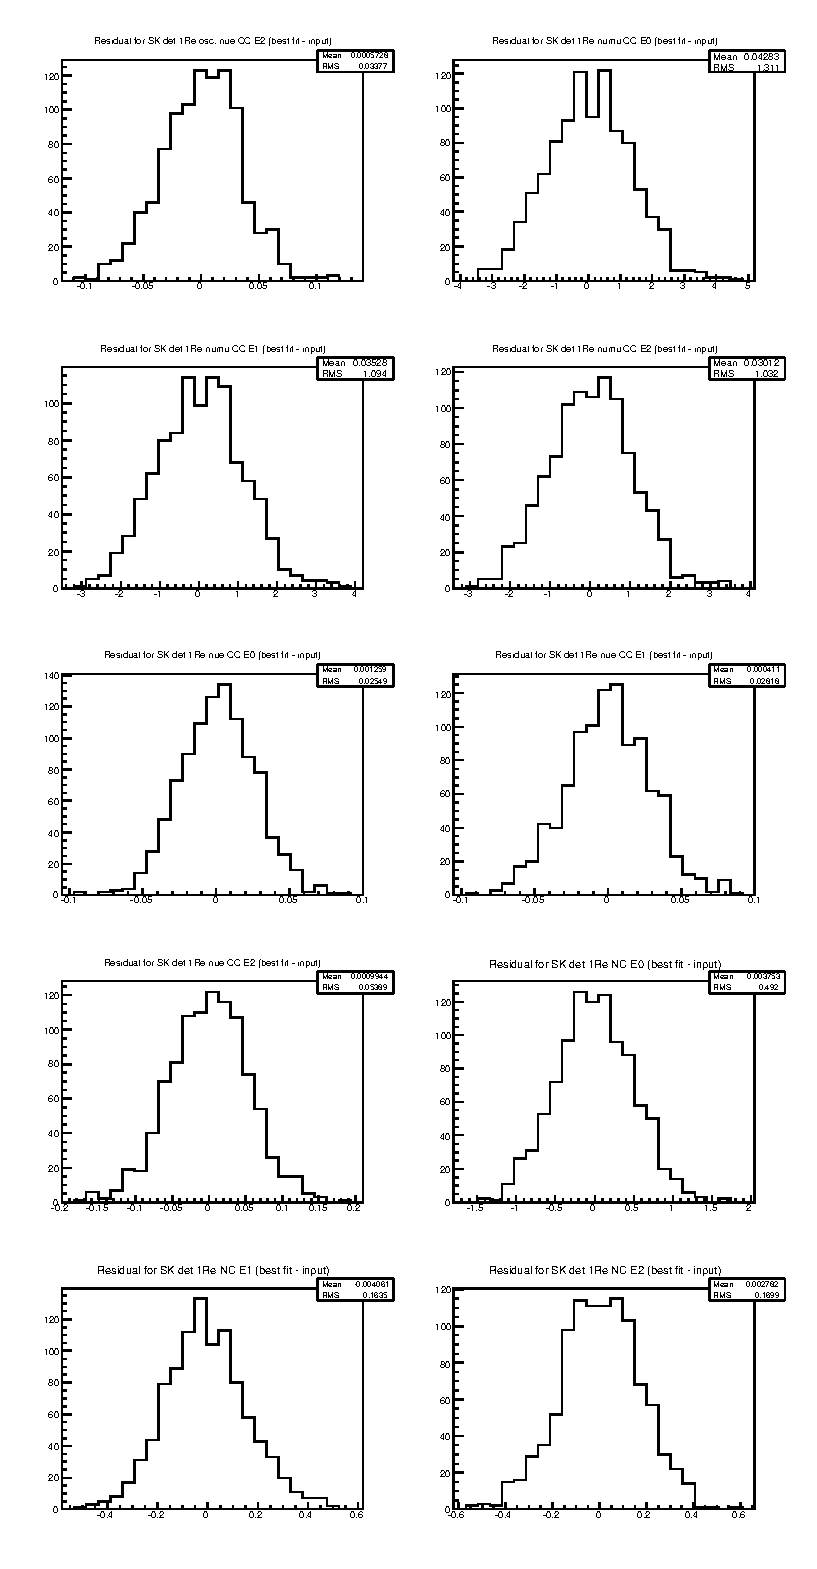
\includegraphics[width=25pc]{images/appendix/fitter_performance/Syst7_residuals_joint_syst_point0.eps}
\caption{
	Distribution of residuals of SK detector (II) systematic parameters in the '4 + 83' fit for oscillation point \# 0. 
 }
\end{figure*}

\begin{figure*}[htbc]	
\center
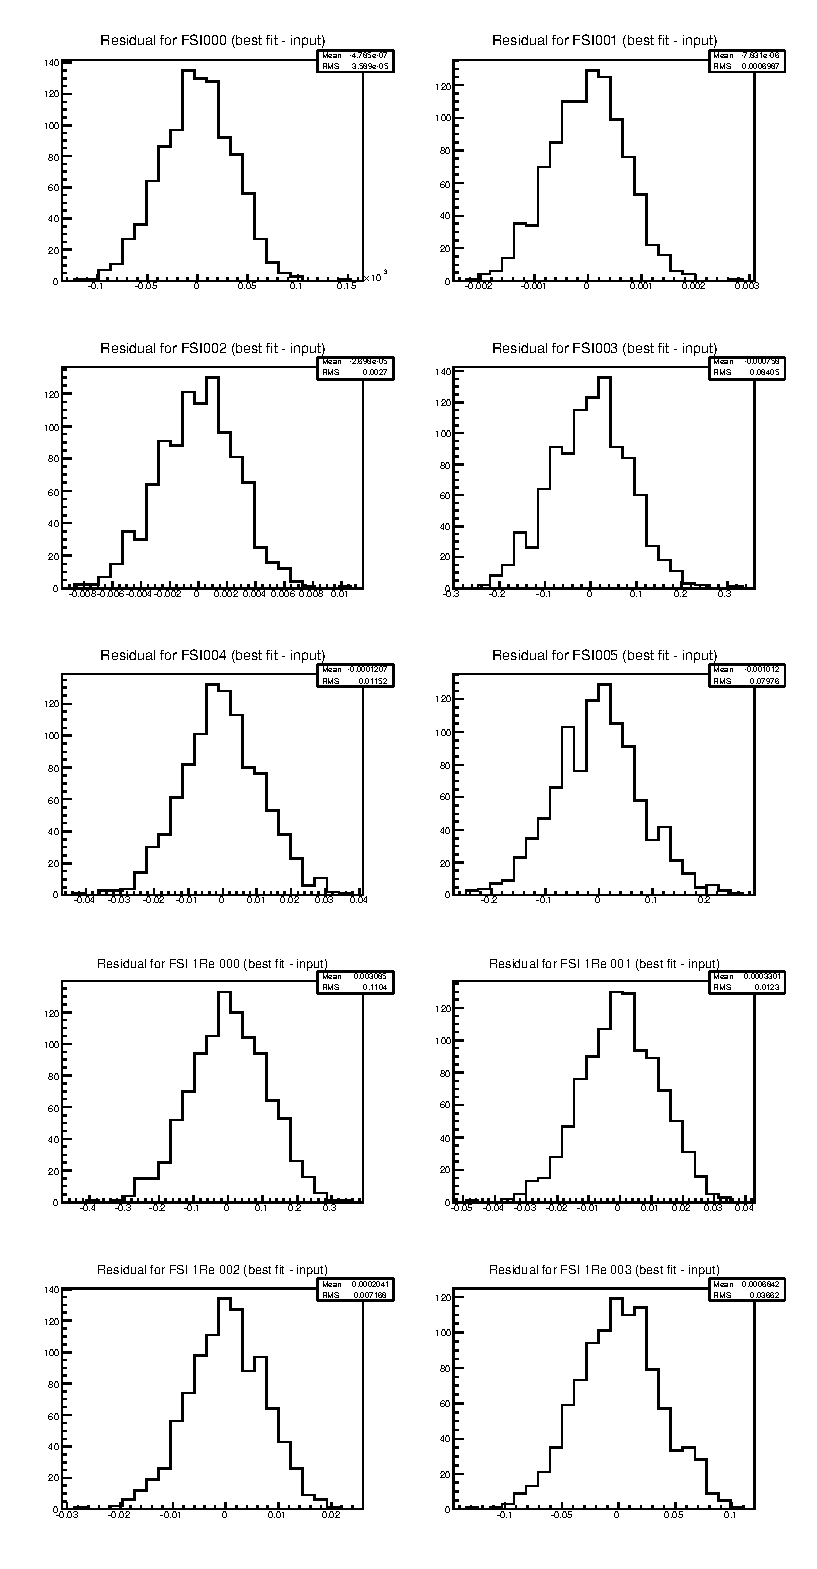
\includegraphics[width=25pc]{images/appendix/fitter_performance/Syst8_residuals_joint_syst_point0.eps}
\caption{
	Distribution of residuals of FSI+SI (I) systematic parameters in the '4 + 83' fit for oscillation point \# 0. 
 }
\end{figure*}

\begin{figure*}[htbc]	
\center
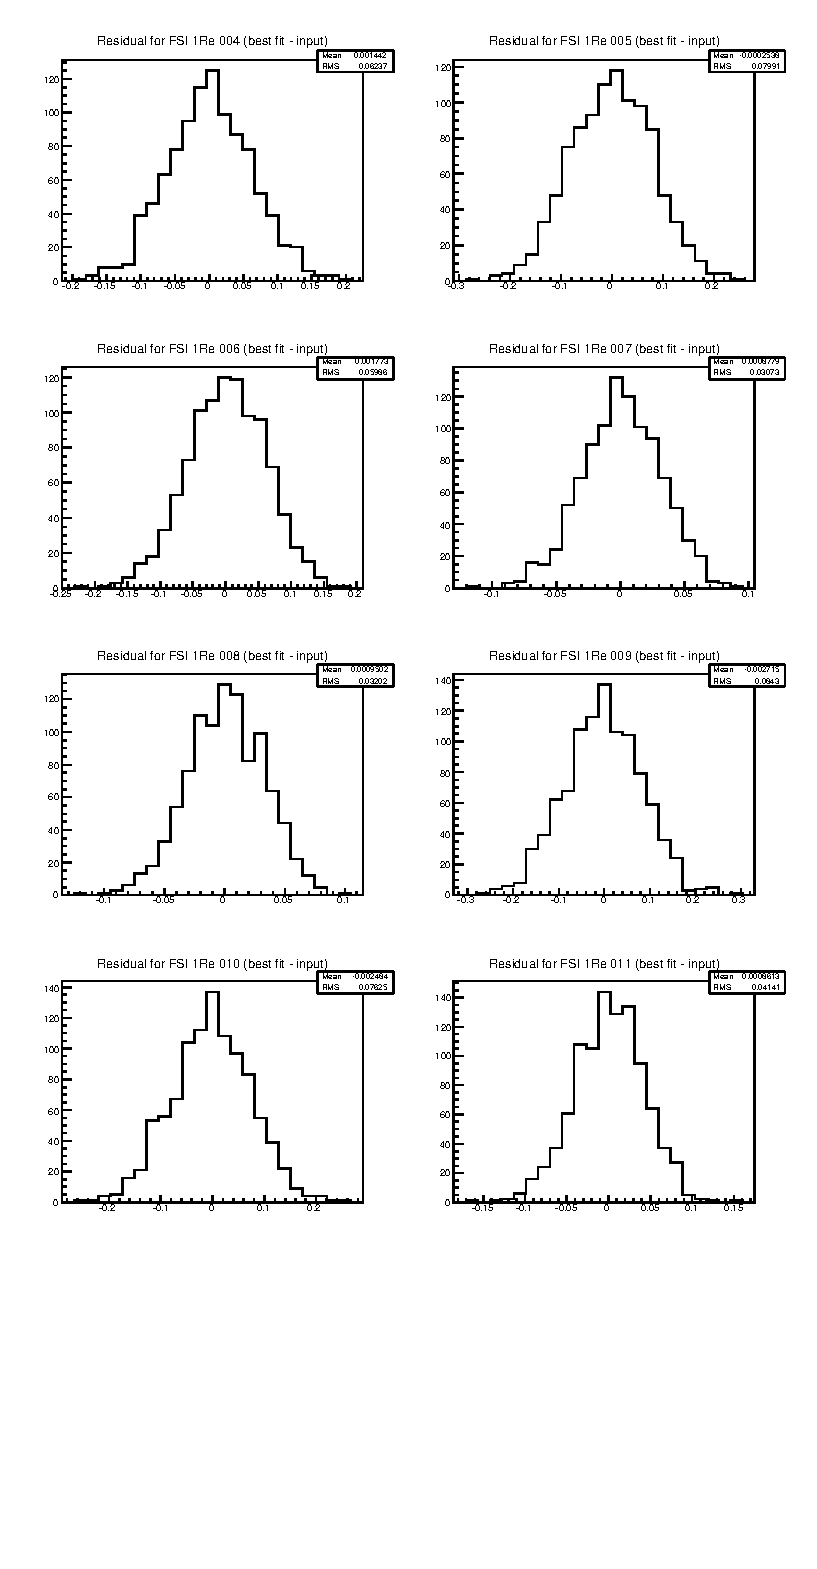
\includegraphics[width=25pc]{images/appendix/fitter_performance/Syst9_residuals_joint_syst_point0.eps}
\caption{
	Distribution of residuals of FSI+SI (I) systematic parameters in the '4 + 83' fit for oscillation point \# 0. 
 }
 \label{fig:residuals_483_syst_last}
\end{figure*}






%%% SUMMARIES

\clearpage

\begin{figure*}[htb]	
\begin{minipage}[t]{0.5\linewidth}
\center
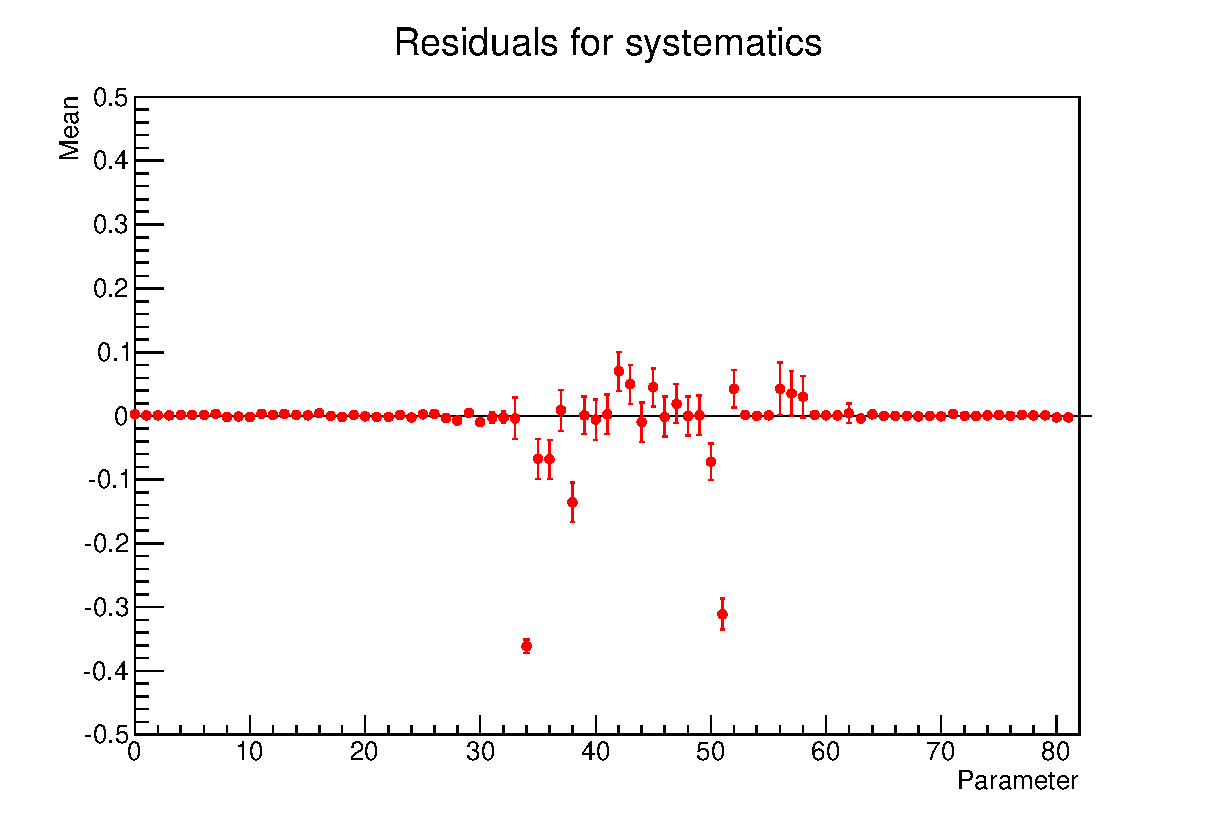
\includegraphics[width=20pc]{images/appendix/fitter_performance/Summary_residuals_joint_syst_point0.eps}
\caption{
	Summary of distribution of residuals of systematic parameters in the '4 + 83' fit for oscillation point \# 0. 
 }
 \label{fig:systematics_point0}
 \end{minipage}
\hspace{0.02\linewidth}	
 \begin{minipage}[t]{0.5\linewidth}
\center
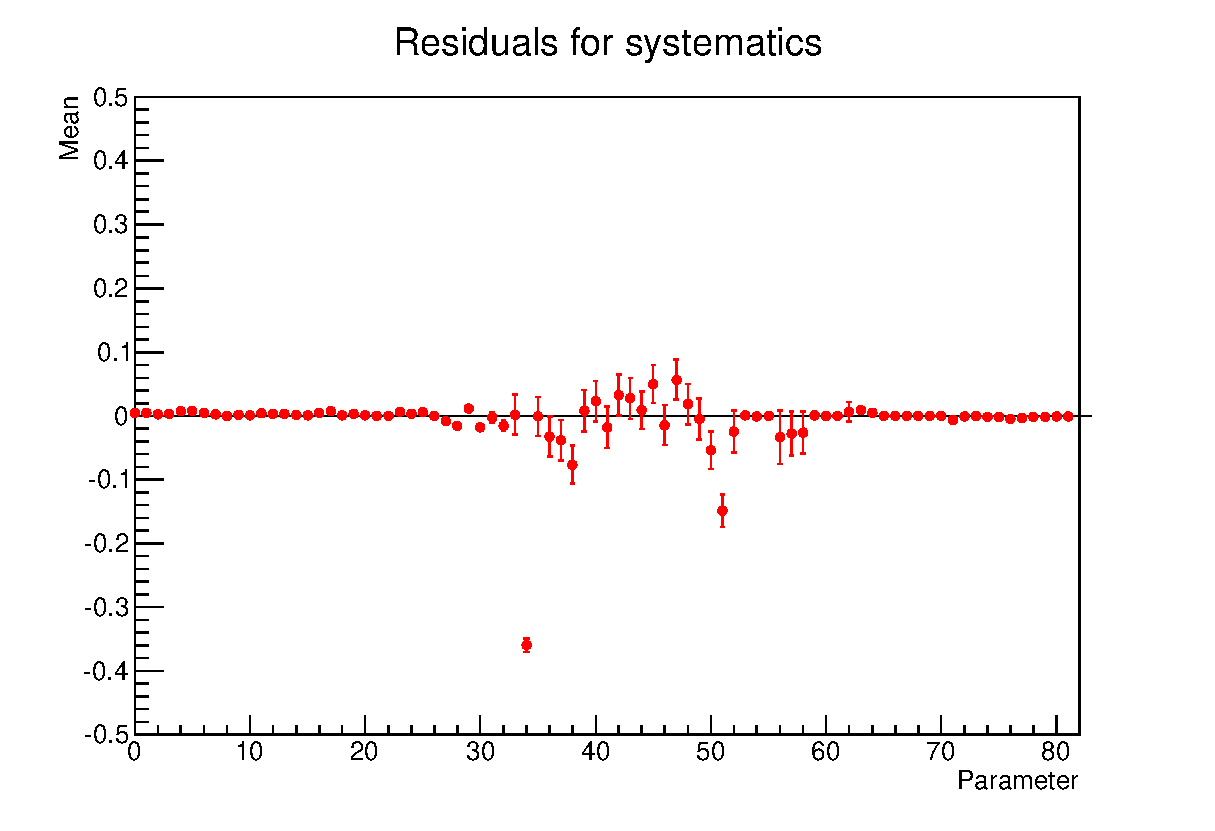
\includegraphics[width=20pc]{images/appendix/fitter_performance/Summary_residuals_joint_syst_point1.eps}
\caption{
	Summary of distribution of residuals of systematic parameters in the '4 + 83' fit for oscillation point \# 1. 
 }
 \end{minipage}

\end{figure*}



\begin{figure*}[htb]	
\begin{minipage}[t]{0.5\linewidth}
\center
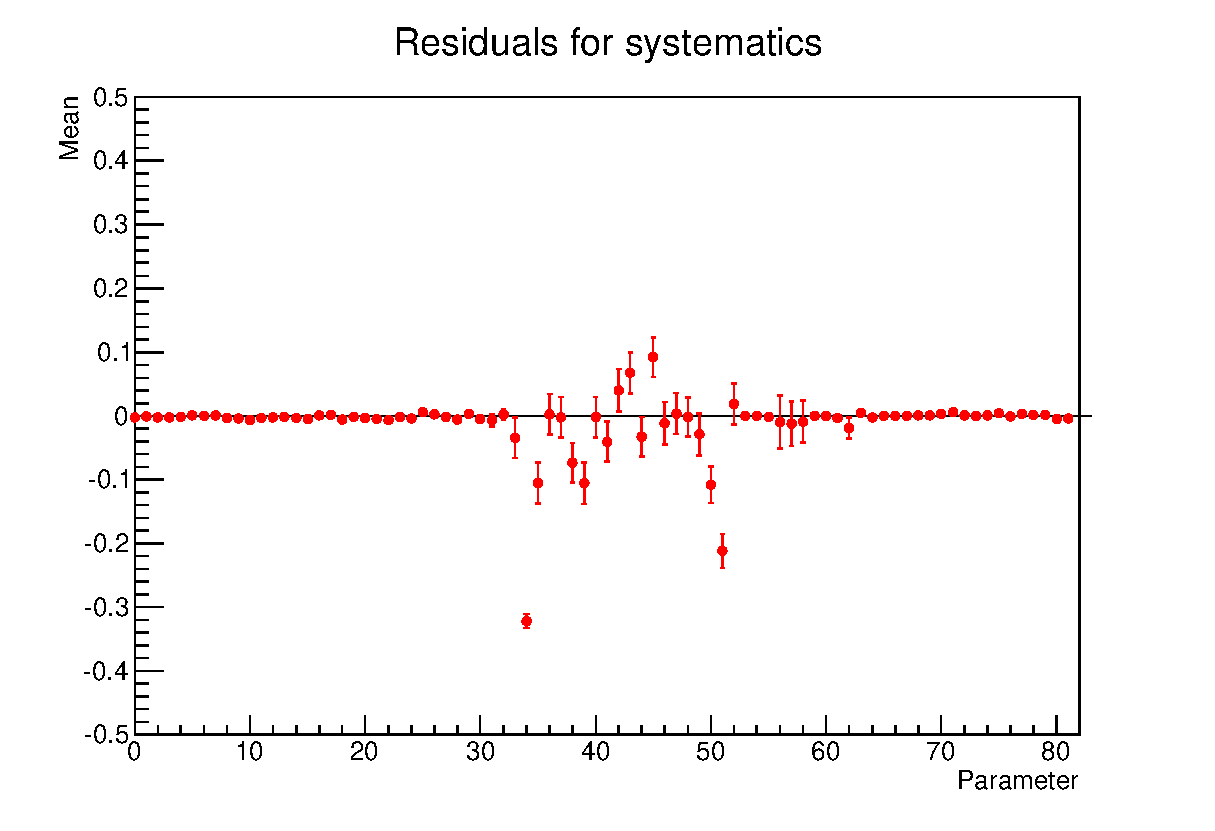
\includegraphics[width=20pc]{images/appendix/fitter_performance/Summary_residuals_joint_syst_point2.eps}
\caption{
	Summary of distribution of residuals of systematic parameters in the '4 + 83' fit for oscillation point \# 2. 
 }
 \label{fig:systematics_point2}
 \end{minipage}
\hspace{0.02\linewidth}	
 \begin{minipage}[t]{0.5\linewidth}
\center
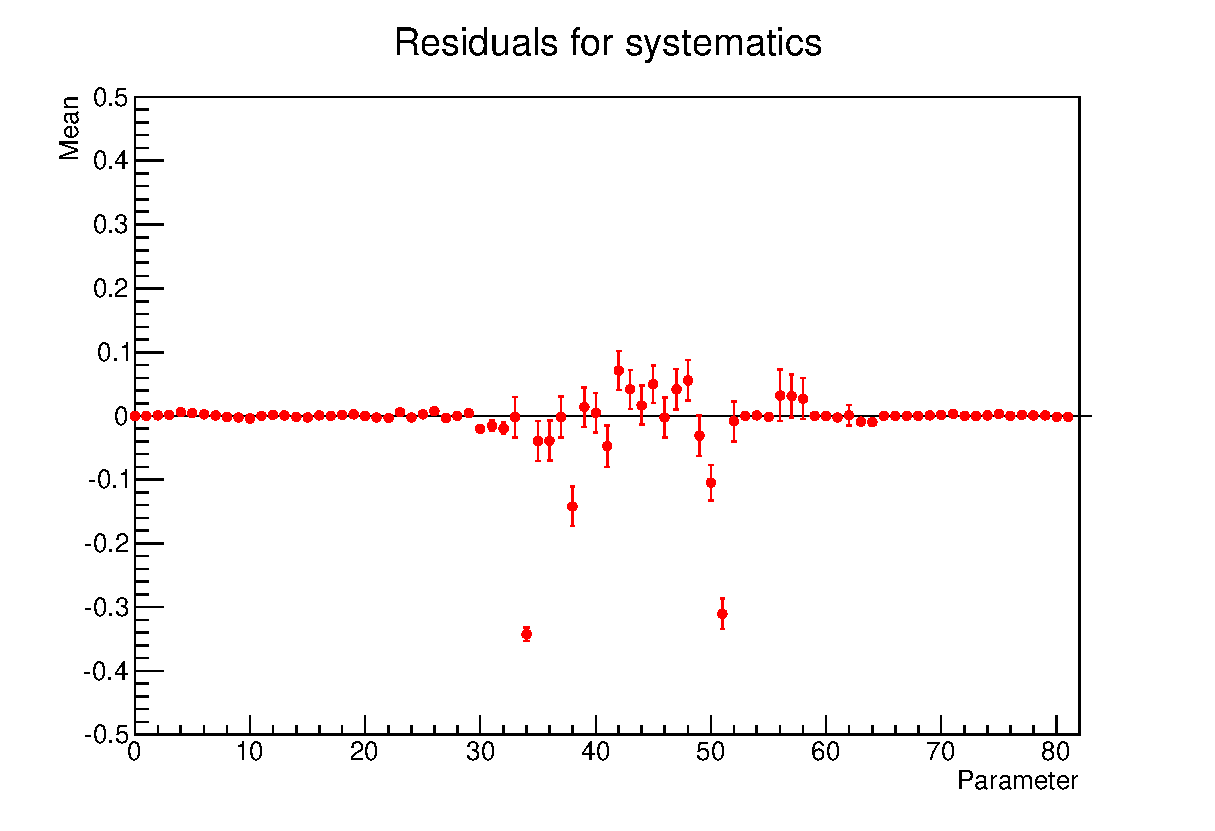
\includegraphics[width=20pc]{images/appendix/fitter_performance/Summary_residuals_joint_syst_point3.eps}
\caption{
	Summary of distribution of residuals of systematic parameters in the '4 + 83' fit for oscillation point \# 3. 
 }
 \end{minipage}

\end{figure*}


\begin{figure*}[htb]	
\begin{minipage}[t]{0.5\linewidth}
\center
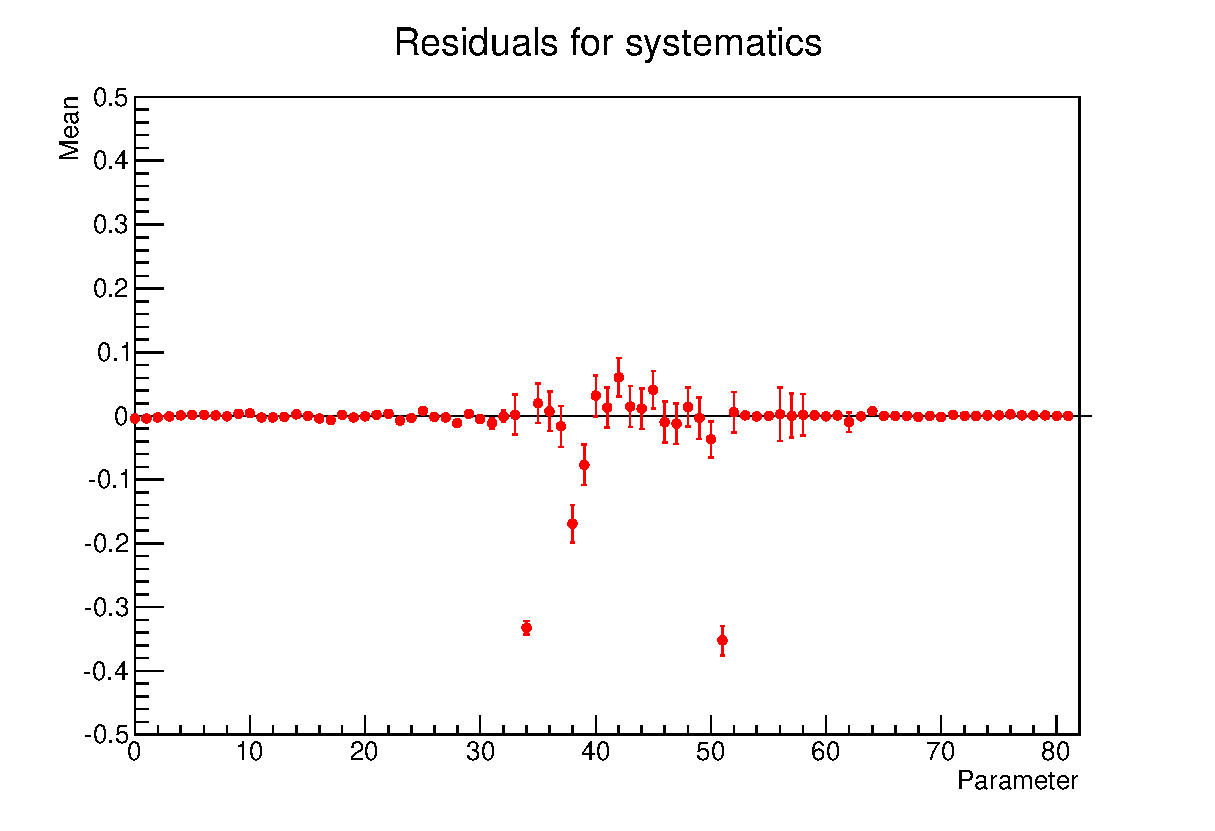
\includegraphics[width=20pc]{images/appendix/fitter_performance/Summary_residuals_joint_syst_point4.eps}
\caption{
	Summary of distribution of residuals of systematic parameters in the '4 + 83' fit for oscillation point \# 4. 
 }
 \label{fig:systematics_point4}
 \end{minipage}
\hspace{0.02\linewidth}	
 \begin{minipage}[t]{0.5\linewidth}
\center
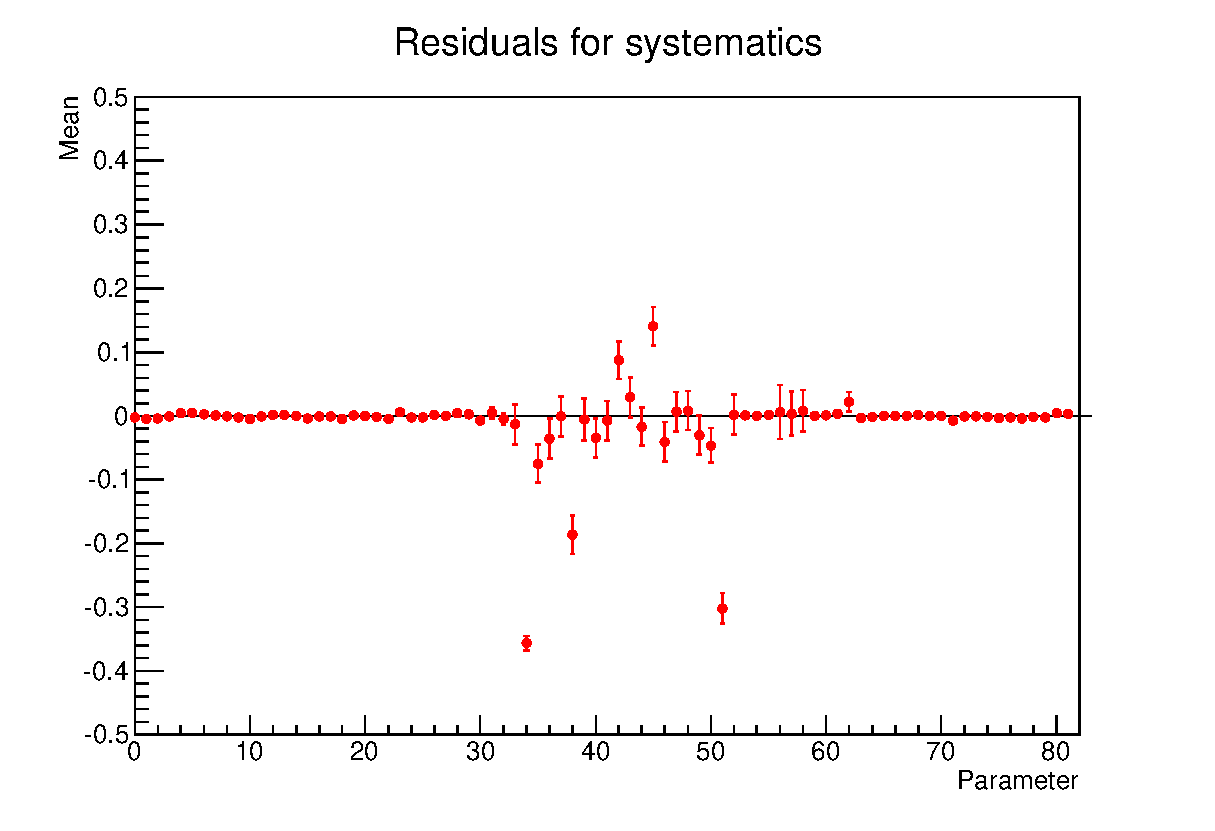
\includegraphics[width=20pc]{images/appendix/fitter_performance/Summary_residuals_joint_syst_point5.eps}
\caption{
	Summary of distribution of residuals of systematic parameters in the '4 + 83' fit for oscillation point \# 5. 
 }
 \end{minipage}

\end{figure*}


\begin{figure*}[htb]	
\begin{minipage}[t]{0.5\linewidth}
\center
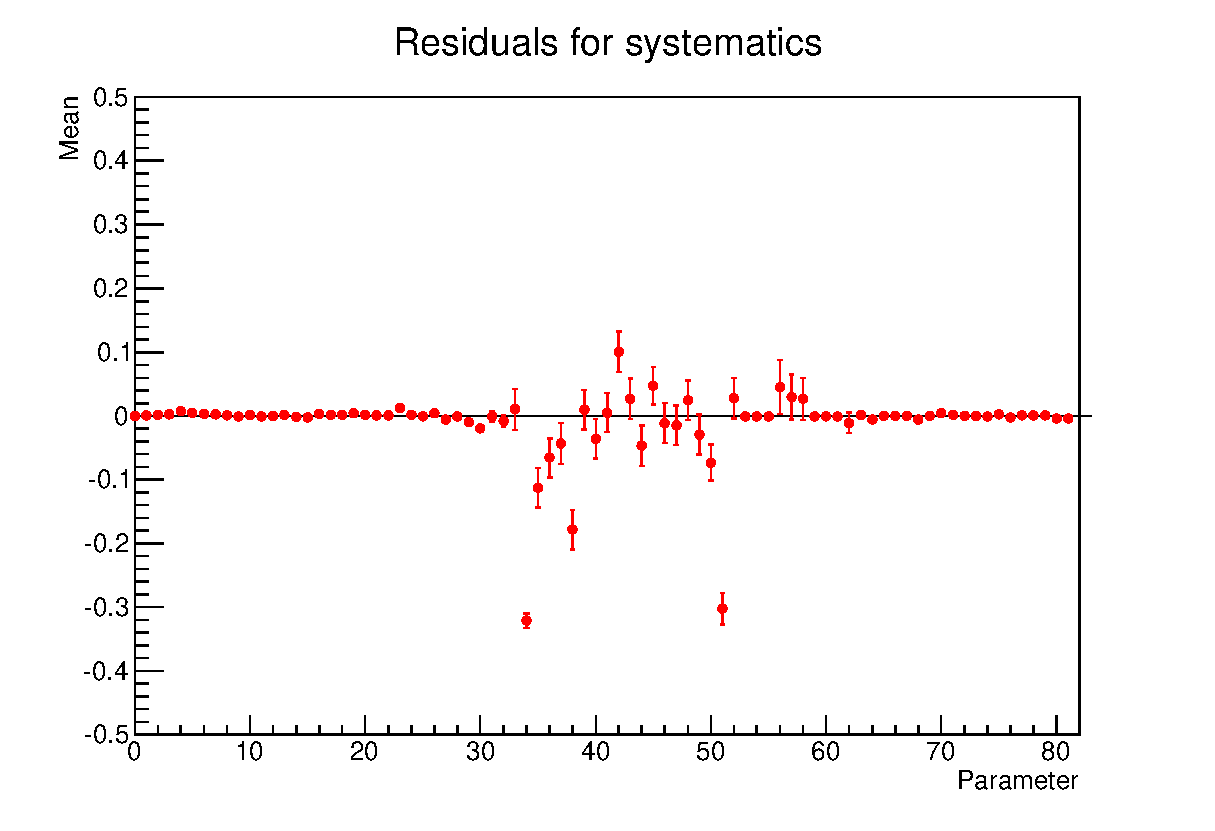
\includegraphics[width=20pc]{images/appendix/fitter_performance/Summary_residuals_joint_syst_point6.eps}
\caption{
	Summary of distribution of residuals of systematic parameters in the '4 + 83' fit for oscillation point \# 6. 
 }
 \label{fig:systematics_point6}
 \end{minipage}
\hspace{0.02\linewidth}	
 \begin{minipage}[t]{0.5\linewidth}
\center
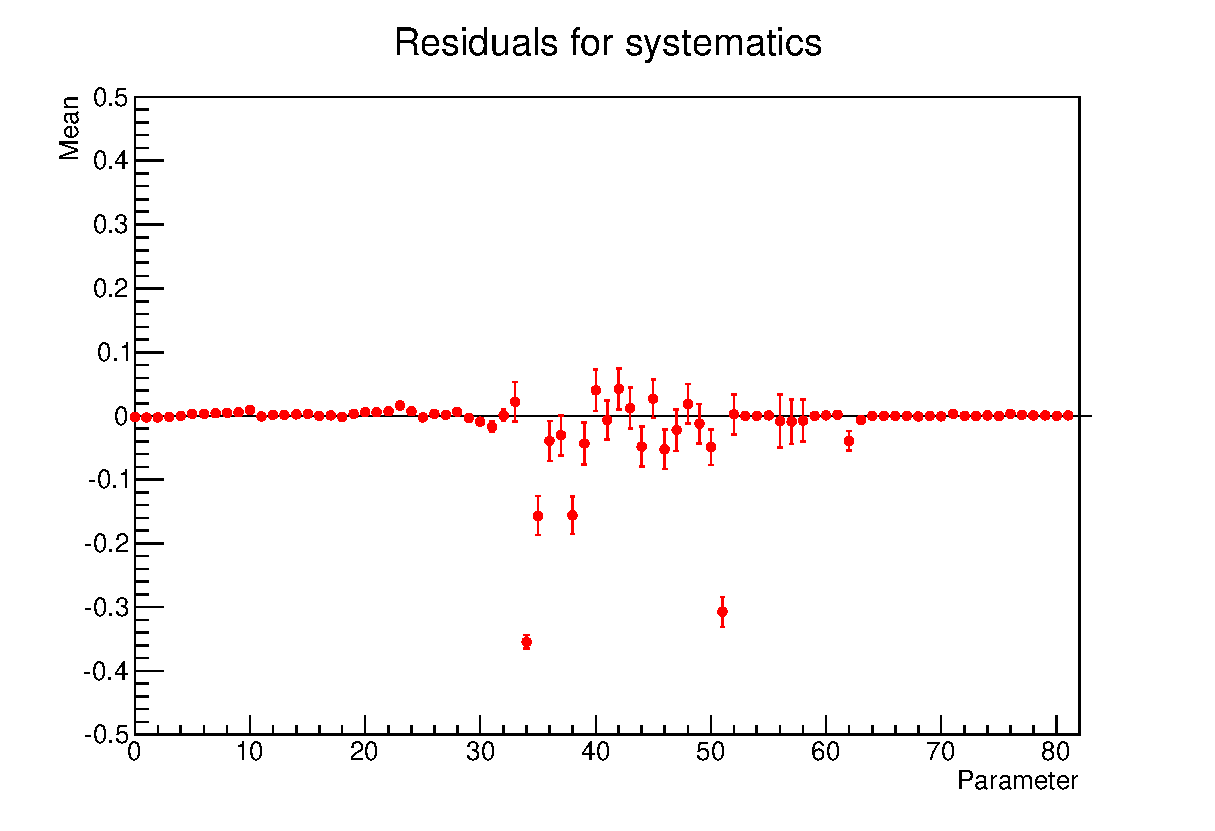
\includegraphics[width=20pc]{images/appendix/fitter_performance/Summary_residuals_joint_syst_point7.eps}
\caption{
	Summary of distribution of residuals of systematic parameters in the '4 + 83' fit for oscillation point \# 7. 
 }
 \end{minipage}

\end{figure*}


\begin{figure*}[htb]	
\begin{minipage}[t]{0.5\linewidth}
\center
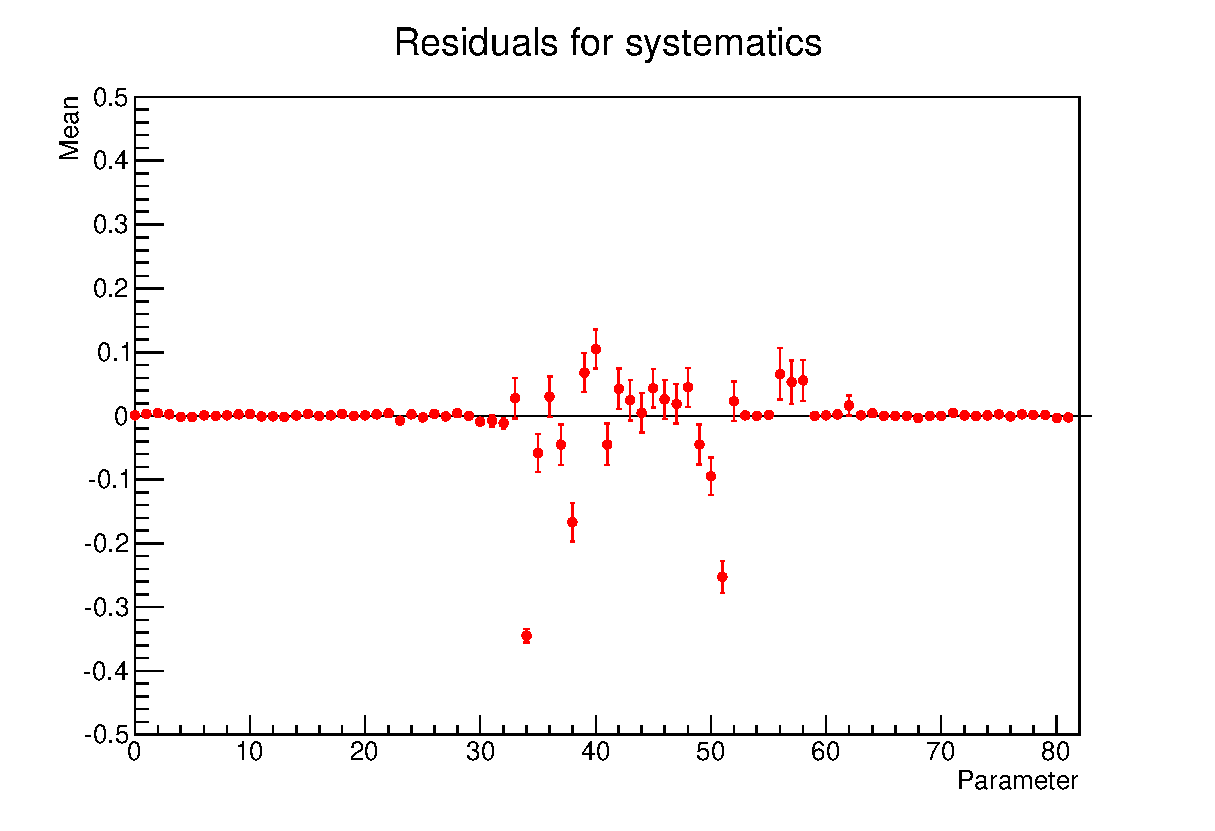
\includegraphics[width=20pc]{images/appendix/fitter_performance/Summary_residuals_joint_syst_point8.eps}
\caption{
	Summary of distribution of residuals of systematic parameters in the '4 + 83' fit for oscillation point \# 8. 
 }
 \label{fig:systematics_point8}
 \end{minipage}
\hspace{0.02\linewidth}	
 \begin{minipage}[t]{0.5\linewidth}
\center
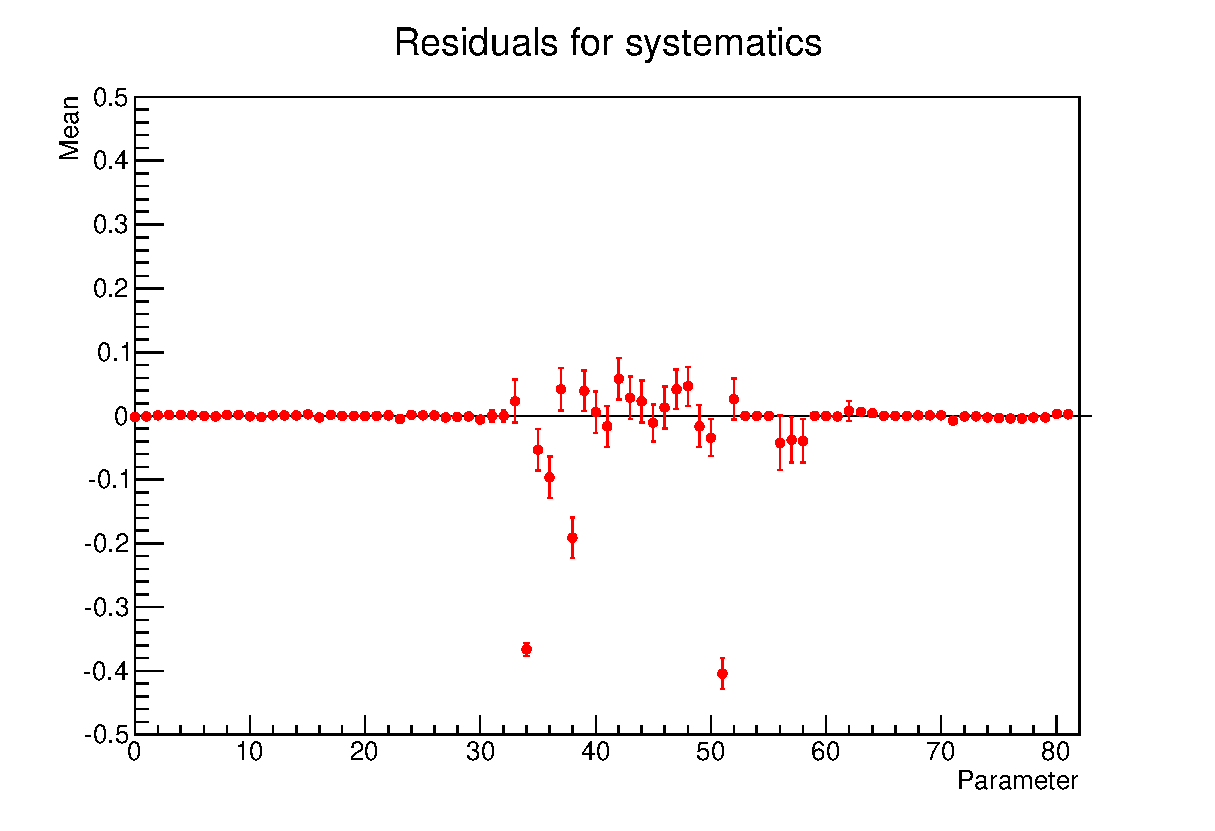
\includegraphics[width=20pc]{images/appendix/fitter_performance/Summary_residuals_joint_syst_point9.eps}
\caption{
	Summary of distribution of residuals of systematic parameters in the '4 + 83' fit for oscillation point \# 9. 
 }
 \end{minipage}
 \label{fig:systematics_point9}
\end{figure*}


\clearpage

\section{3.010$\times$10$^{20}$ POT fake dataset fits}
\label{app:fake_dataset_fits}

In order to validate the joint 3-flavour analysis, fake single $\mu$-like ring and 
single e-like ring datasets were created for an equivalent exposure of 3.010$\times$10$^{20}$ POT. 
Two different studies were done: 1) using data sets without statistical fluctuations and 2) using datasets with statistical fluctuations. 
For each of these datasets, the true oscillation parameters, 
mass hierarchy, systematic variations and the generated numbers of single $\mu$-like ring and 
single e-like ring events are shown in Tab.\ \ref{tab:toymc_fits:best_fit_values} for datasets with no statistical fluctuations and in 
Tab.\ \ref{tab:toymc_fits:best_fit_values_realistic} for datasets with statistical fluctuations. 
Each of these datasets was fitted three times: 1) using the {\em VaLOR} joint 3-flavour oscillation analysis,
2) with the {\em VaLOR} stand-alone $\nu_{e}$ appearance analysis and 3) with the {\em VaLOR} stand-alone $\nu_{\mu}$-disappearance analysis.
The best-fit values of the oscillation parameters for those fits 
are also given in Tables \ref{tab:toymc_fits:best_fit_values} and \ref{tab:toymc_fits:best_fit_values_realistic},  
along with the goodness-of-fit and the number of single $\mu$-like ring and single e-like ring events
computed from the best-fit spectra. The corresponding figures are \ref{fig:toymc0_dchisq_Dmsq}-\ref{fig:toymc5_confreg_sinsqtheta23_sinsqtheta13} for fake data sets with no 
statistical fluctuations and \ref{fig:toymc6_1Rmu_bestfit_spectrum}-\ref{fig:toymc7_pulls} for fake data sets with statistical fluctuations. 

The profile $\Delta\chi^2$ distribution is also presented for the fit of each fake dataset as a function 
of each of the oscillation parameters $|\Delta m^{2}|$, $\sin^{2}\theta_{23}$, $\sin^{2}\theta_{13}$ and $\delta_{CP}$. 
In addition, the 68\% and 90\% CL regions are given in the following four 2-dimensional oscillation parameter spaces: 
($\sin^{2}\theta_{23}$, $|\Delta m^{2}|$), 
($\sin^{2}\theta_{13}$, $|\Delta m^{2}|$),
($\sin^{2}\theta_{13}$, $\delta_{CP}$) and
($\sin^{2}\theta_{23}$, $\sin^{2}\theta_{13}$).

In all profile $\Delta\chi^2$ and confidence region plots shown for the joint 3-flavour analysis,
the value of $\chi^2$ was minimized with respect to all 83 nuisance parameters
and the oscillation parameters from $|\Delta m^{2}|$, $\sin^{2}\theta_{23}$, $\sin^{2}\theta_{13}$ and $\delta_{CP}$ not 
shown on the plot (as explained in App.\ \ref{app:solar}, $\sin^{2}\theta_{12}$ and $\delta m^{2}$ have a negligible effect and they are fixed to 
$0.311$ and $7.5\times$10$^{-5}$ eV$^{2}$/c$^{4}$ respectively for all the joint and stand-alone 
$\nu_{e}$-appearance and $\nu_{\mu}$-disappearance analyses).
In the profile $\Delta\chi^2$ and confidence region plots shown for 
the stand-alone $\nu_{e}$ appearance analysis, $\sin^{2}\theta_{23}$ and $|\Delta m^{2}|$ are also fixed to 0.5 and 
2.4$\times$10$^{-3}$ eV$^{2}$/c$^{4}$ respectively, and the $\chi^2$ was minimized with respect to $\sin^{2}\theta_{13}$, 
$\delta_{CP}$ and all 69 nuisance parameters relevant for that analysis. 
Similarly, for $\nu_{\mu}$ disappearance, $\sin^{2}\theta_{13}$ and $\delta_{CP}$ are fixed to 0.025 and 0 respectively,
and the $\chi^2$ was minimized with respect to $\sin^{2}\theta_{23}$, $|\Delta m^{2}|$ and all 57 nuisance parameters
relevant to that analysis. These fixed values of the oscillation parameters are the same as those used in the T2K published results. 

Confidence regions are found with respect to a $\chi^{2}$ global minimum reported in Tab.\ \ref{tab:toymc_fits:best_fit_values}
or in Tab.\ \ref{tab:toymc_fits:best_fit_values_realistic}
(except for the stand-alone $\nu_{e}$ appearance result in ($\sin^{2}\theta_{13}$, $\delta_{CP}$) space
where the raster scan was used) using the constant-$\Delta\chi^{2}$ method (see Section \ref{sec:neutrino_oscillation_fitting}).

The following color scheme is used for all plots:
\begin{itemize}
\item green $\rightarrow$ true,
\item black $\rightarrow$ {\em VaLOR} joint 3-flavour oscillation analysis,
\item red   $\rightarrow$ {\em VaLOR} stand-alone $\nu_{e}$ appearance analysis, and
\item blue  $\rightarrow$ {\em VaLOR} stand-alone $\nu_{\mu}$ disappearance analysis.
\end{itemize}


From the results of the joint oscillation analysis in these fake dataset fits the following conclusions can be extracted:

\begin{enumerate}
\item{The results show in general a good recovery of the true input value of the oscillation parameters at the best fit point. } 
\item{There is no sensitivity to $\delta_{CP}$ at current POT as can be observed for instance in Fig.\ \ref{fig:toymc0_dchisq_deltacp}. }
\item{As expected, when a best fit value of $\delta_{CP}$ is different to the true one, this can cause, due to their intrinsic degeneracy, 
a bias in the best fit value of $sin^{2}\theta_{13}$.  This bias in  $sin^{2}\theta_{13}$ translates, in turn, into a bias in $sin^{2}\theta_{23}$.  }
\item{Other interesting confidence regions in oscillation parameter spaces different to the usual ones, 
    ($\sin^{2}\theta_{13}$, $|\Delta m^{2}|$) and  ($\sin^{2}\theta_{23}$, $\sin^{2}\theta_{13}$), 
    can be studied with satisfactory results when using the joint oscillation analysis. }
\item{In this work, the difference in the confidence regions for the disappearance oscillation parameters 
($\sin^{2}\theta_{23}$, $|\Delta m^{2}|$) with different mass hierarchies was studied for the first time 
(compare Fig.\ \ref{fig:toymc0_confreg_sinsqtheta23_Dmsq} with Fig.\ \ref{fig:toymc5_confreg_sinsqtheta23_Dmsq}).} 
%\label{fig:toymc5_confreg_sinsqtheta23_Dmsq}
\item{Using the joint oscillation analysis it is also possible to investigate the octant degeneracy 
    in $\sin^{2}\theta_{23}$ as the single e-like ring sample has been added (see for instance Figs.\ \ref{fig:toymc1_dchisq_sinsqtheta23}, 
    \ref{fig:toymc1_confreg_sinsqtheta23_Dmsq}  and  \ref{fig:toymc1_confreg_sinsqtheta23_sinsqtheta13}) . }
\end{enumerate}

Comparing the results of stand-alone analyses with the ones for the joint analysis:

\begin{enumerate}
\item{A larger uncertainty is found for $\sin^{2}\theta_{13}$ with the joint analysis (wider $\chi^2$ profiles in 
    Figs.\ \ref{fig:toymc0_dchisq_sinsqtheta13}, 
    \ref{fig:toymc1_dchisq_sinsqtheta13},  
    \ref{fig:toymc2_dchisq_sinsqtheta13},  
    \ref{fig:toymc3_dchisq_sinsqtheta13},  
    \ref{fig:toymc4_dchisq_sinsqtheta13} and  
    \ref{fig:toymc5_dchisq_sinsqtheta13})   
    because its correlations with $\sin^{2}\theta_{23}$ and $\delta_{CP}$ are taken into account. }
\item{For the stand-alone appearance analysis, biases appear in the best-fit value of $\sin^{2}\theta_{13}$ when the value of $\sin^{2}\theta_{23}$ or $\delta_{CP}$ 
does not correspond to the value assumed as prior (typically $\sin^{2}\theta_{23}$=0.5 and $\delta_{CP}$=0), as shown in 
Table \ref{tab:toymc_fits:best_fit_values} for sets \#1 and \#3. 
Fitting them in the joint analysis solves this problem. }
\item{The confidence regions in the 2-dimensional oscillation parameter spaces obtained with the joint analysis are comparable in size with 
    the ones obtained with stand-alone analyses, because despite the fact that more parameters are included in the fit, this is compensated by the 
    extra information added when working simultaneously with 
    the single $\mu$-like ring and single e-like ring samples. }
\end{enumerate}


\begin{table}[htb]
\small
\centering
\begin{tabular}{@{}| c | l | c  c  c  c| c | c  c  | c | |@{}}
\hline
Set & Fit  & $|\Delta m^2|$  & sin$^2\theta_{23}$ & sin$^2\theta_{13}$  & $\delta_{CP}$  &  MH & N$_{SK}^{1R\mu}$ & N$_{SK}^{1Re}$ & Figures  \\
 &   & ( $\times$10$^{-3}$ eV$^{2}$/c$^{4}$) &  &   &  &   &  & &  \\
\hline
0  & true                      & {\bf 2.36 }   & {\bf 0.5}   & {\bf 0.025}   & {\bf 0.0}  & {\bf Normal} & {\bf 59.745}   & {\bf 10.981}   &  \\
   & fit (joint)               & 2.361          & 0.500      & 0.023      & -0.279   & (fixed)    & 59.742     & 10.975   &  \ref{fig:toymc0_dchisq_Dmsq} - \ref{fig:toymc0_confreg_sinsqtheta23_sinsqtheta13} \\
   & fit ($\nu_{e}$ app.)      & --                             & --         & 0.025      & 0(fixed)  &     & --         & 10.982     &  \\
   & fit ($\nu_{\mu}$ disapp.) & 2.361         & 0.497      & --         & --       &   & 59.759      & --       & \\
\hline
1  & true                      & {\bf 2.36 }   & {\bf 0.38}   & {\bf 0.025}   & {\bf 0.0}   & {\bf Normal}  & {\bf 69.475}   & {\bf 9.199}   &  \\
   & fit (joint)               & 2.360         & 0.380      & 0.025      & 0.014    & (fixed)   & 69.474      & 9.202      &  \ref{fig:toymc1_dchisq_Dmsq} - \ref{fig:toymc1_confreg_sinsqtheta23_sinsqtheta13}  \\
   & fit ($\nu_{e}$ app.)      & --                             & --         & 0.019      & 0(fixed)   &     & --         & 9.200       & \\
   & fit ($\nu_{\mu}$ disapp.) & 2.360          & 0.380      & --         & --  &         & 69.471      & --          & \\
\hline
2  & true                      & {\bf 2.36 }   & {\bf 0.5}   & {\bf 0.015}   & {\bf 0.0}   & {\bf Normal}  & {\bf 59.688}   & {\bf 7.993}    & \\
   & fit (joint)               & 2.360          & 0.506      & 0.017      & 0.322   & (fixed)    & 59.676      & 7.997       & \ref{fig:toymc2_dchisq_Dmsq} - \ref{fig:toymc2_confreg_sinsqtheta23_sinsqtheta13} \\
   & fit ($\nu_{e}$ app.)      & --                             & --         & 0.015      & 0(fixed)   &   & --         & 7.991       & \\
   & fit ($\nu_{\mu}$ disapp.) & 2.360          & 0.500      & --         & --   &        & 59.726      & --          & \\
\hline
3  & true                      & {\bf 2.36 }   & {\bf 0.5}   & {\bf 0.025}   & {\bf $-\pi/2$} & {\bf Normal}   & {\bf 60.006}   & {\bf 12.838}    &\\
   & fit (joint)               & 2.360         & 0.529      & 0.024      & -1.522  & (fixed)     & 60.017      & 12.848       & \ref{fig:toymc3_dchisq_Dmsq} - \ref{fig:toymc3_confreg_sinsqtheta23_sinsqtheta13}\\
   & fit ($\nu_{e}$ app.)      & --                             & --         & 0.031      & 0(fixed)   &     & --         & 12.860       & \\
   & fit ($\nu_{\mu}$ disapp.) & 2.349         & 0.497      & --         & --    &     & 60.018      & --          & \\
\hline
4  & true                      & {\bf 2.2 }   & {\bf 0.5}   & {\bf 0.025}   & {\bf 0.0}  & {\bf Normal}  & {\bf 64.195}   & {\bf 10.956}    & \\
   & fit (joint)               & 2.200         & 0.527      & 0.024      & 0.076   & (fixed)    & 64.188      & 10.955       & \ref{fig:toymc4_dchisq_Dmsq} - \ref{fig:toymc4_confreg_sinsqtheta23_sinsqtheta13}\\
   & fit ($\nu_{e}$ app.)      & --                             & --         & 0.025      & 0(fixed)     &   & --         & 10.962       & \\
   & fit ($\nu_{\mu}$ disapp.) & 2.199          & 0.501      & --         & --   &      & 64.206      & --          &\\
\hline
5  & true                      & {\bf 2.36 }   & {\bf 0.5}   & {\bf 0.025}   & {\bf 0.0}  & {\bf Inverted}  & {\bf 59.577}   & {\bf 9.559}    & \\
   & fit (joint)               & 2.359         & 0.496      & 0.022      & -0.445    & (fixed)   & 59.583      & 9.558       & \ref{fig:toymc5_dchisq_Dmsq} - \ref{fig:toymc5_confreg_sinsqtheta23_sinsqtheta13}\\
   & fit ($\nu_{e}$ app.)      & --                             & --         & 0.025      & 0(fixed)    &     & --         & 9.560       & \\
   & fit ($\nu_{\mu}$ disapp.) & 2.361        & 0.496      & --         & --     &      & 59.593      & --          & \\
 
\hline
\end{tabular}
\caption{
  True input values (shown in bold) and VALOR best-fit values for a test ensemble of 6 fake datasets with no statistical fluctuations. 
}
\label{tab:toymc_fits:best_fit_values}
\end{table}

\clearpage
%
%
% ..............................................
% Fake dataset #0
%
%


%
% delta\chisq and contours
%

\begin{figure*}[htb]

\begin{minipage}[t]{0.22\linewidth}
\center
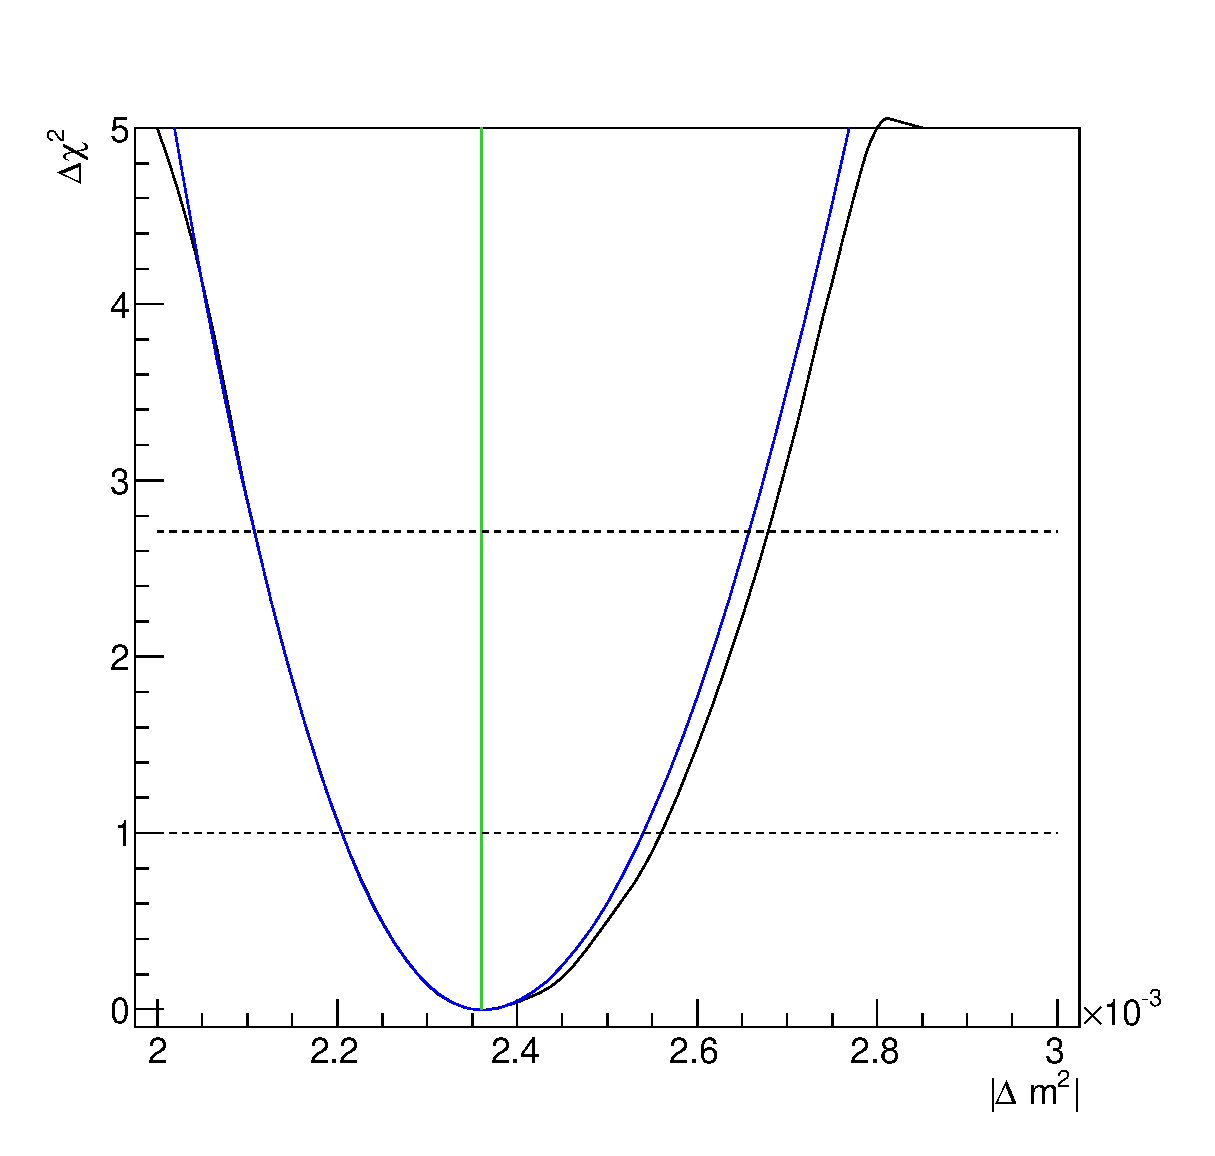
\includegraphics[width=9pc]{./images/appendix/fake_dataset_fits/fake_dataset0_chisq_dm23sq_global_min_new.eps}
\caption {
  $\Delta\chi^2$ as function of $|\Delta m^{2}|$ for fake dataset \#0.
  At each point, $\chi^2$ was minimized with respect to 
  $\sin^{2}\theta_{23}$, $\sin^{2}\theta_{13}$, $\delta_{CP}$
  and all relevant nuisance parameters for the joint analysis (black)
  and with respect to $\sin^{2}\theta_{23}$ and all relevant nuisance
  parameters for the disappearance analysis (blue).
}
\label{fig:toymc0_dchisq_Dmsq}
\end{minipage}
\hspace{0.02\linewidth}
\begin{minipage}[t]{0.22\linewidth}
\center
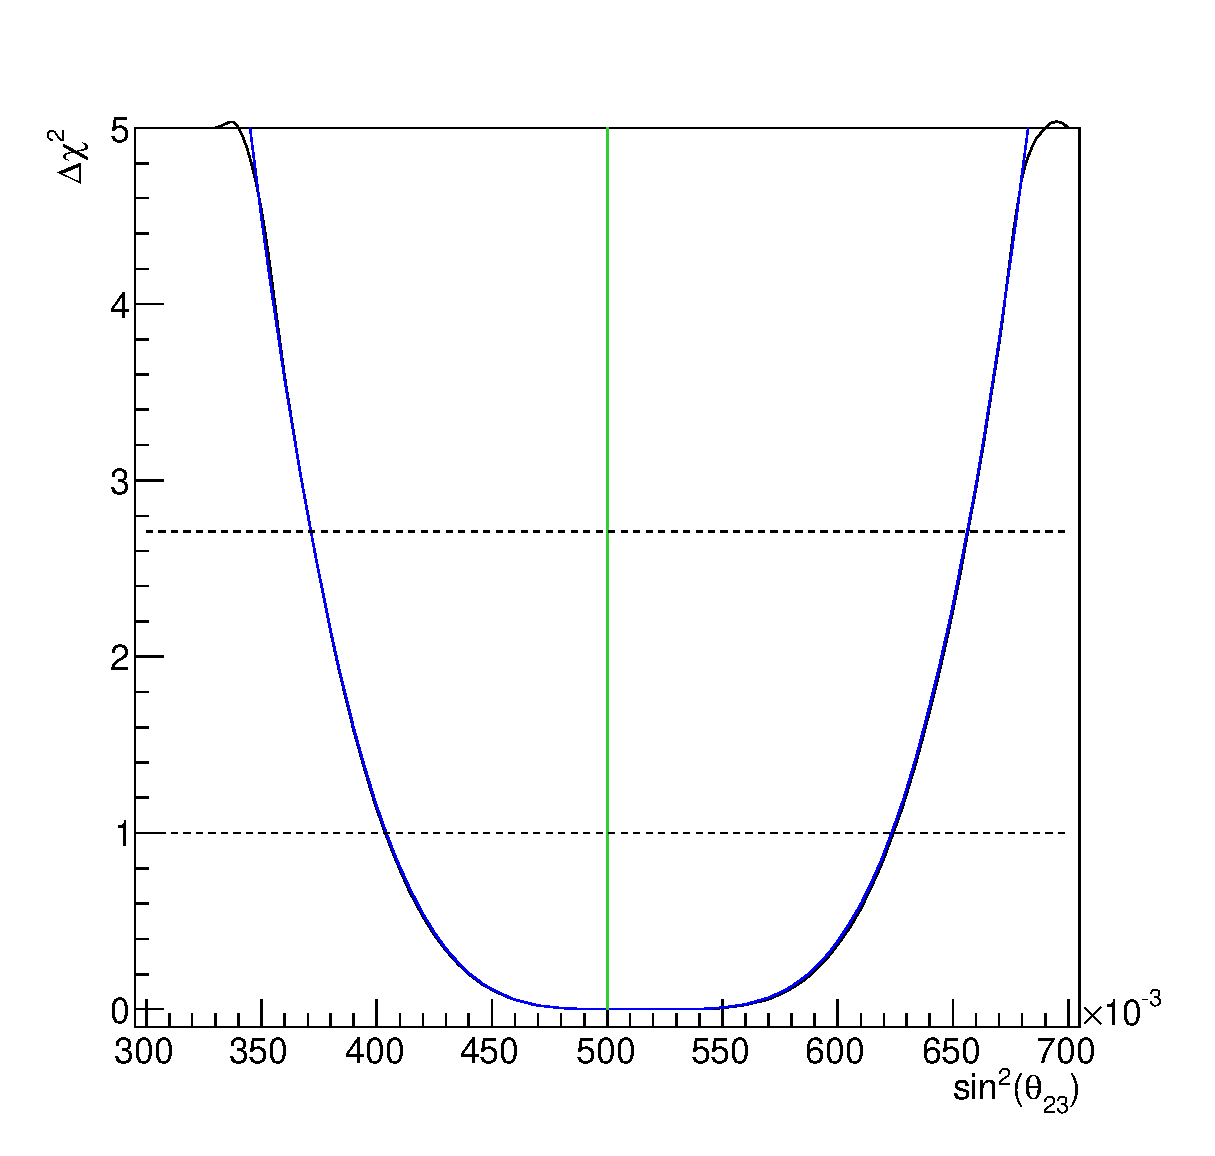
\includegraphics[width=9pc]{./images/appendix/fake_dataset_fits/fake_dataset0_chisq_theta23_global_min_new.eps}
\caption {
  $\Delta\chi^2$ as function of $sin^{2}\theta_{23}$ for fake dataset \#0.
  At each point, $\chi^2$ was minimized with respect to 
  $|\Delta m^{2}|$, $\sin^{2}\theta_{13}$, $\delta_{CP}$
  and all relevant nuisance parameters for the joint analysis (black)
  and with respect to $\sin^{2}\theta_{23}$ and all relevant nuisance
  parameters for the disappearance analysis (blue).
}
\label{fig:toymc0_dchisq_sinsqtheta23}
\end{minipage}
\hspace{0.02\linewidth}
\begin{minipage}[t]{0.22\linewidth}
\center
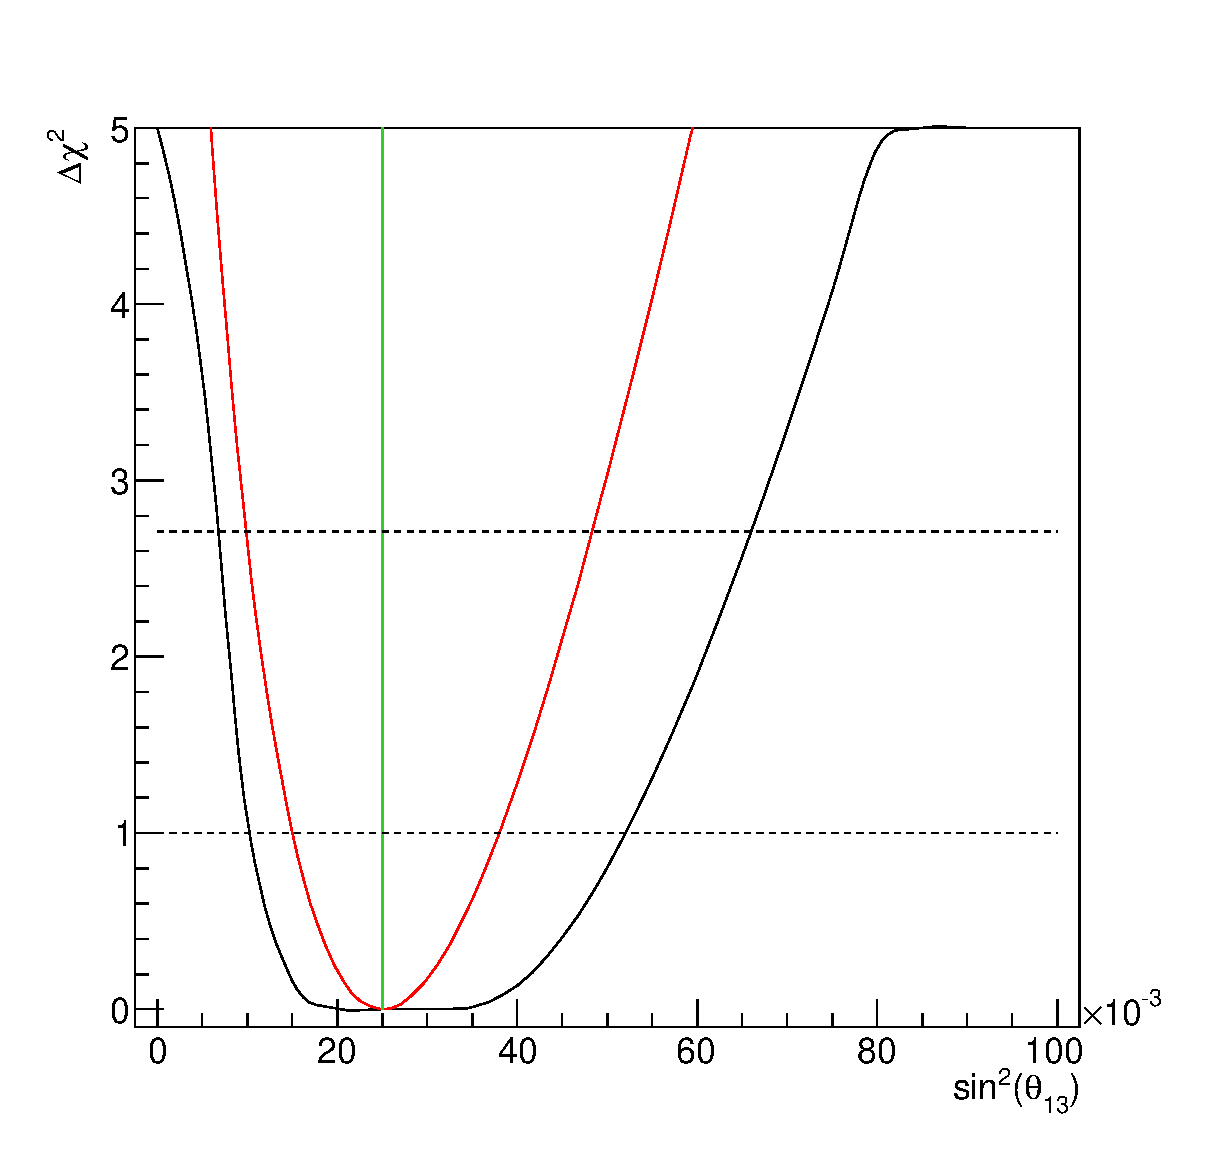
\includegraphics[width=9pc]{./images/appendix/fake_dataset_fits/fake_dataset0_chisq_theta13_global_min_new.eps}
\caption {
  $\Delta\chi^2$ as function of $sin^{2}\theta_{13}$ for fake dataset \#0.
  At each point, $\chi^2$ was minimized with respect to 
  $\sin^{2}\theta_{23}$, $\sin^{2}\theta_{13}$, $\delta_{CP}$
  and all relevant nuisance parameters for the joint analysis (black)
  and with respect to all relevant nuisance parameters 
  ($\delta_{CP}$ is fixed to 0) for the appearance analysis (red).
}
\label{fig:toymc0_dchisq_sinsqtheta13}
\end{minipage}
\hspace{0.02\linewidth}
\begin{minipage}[t]{0.22\linewidth}
\center
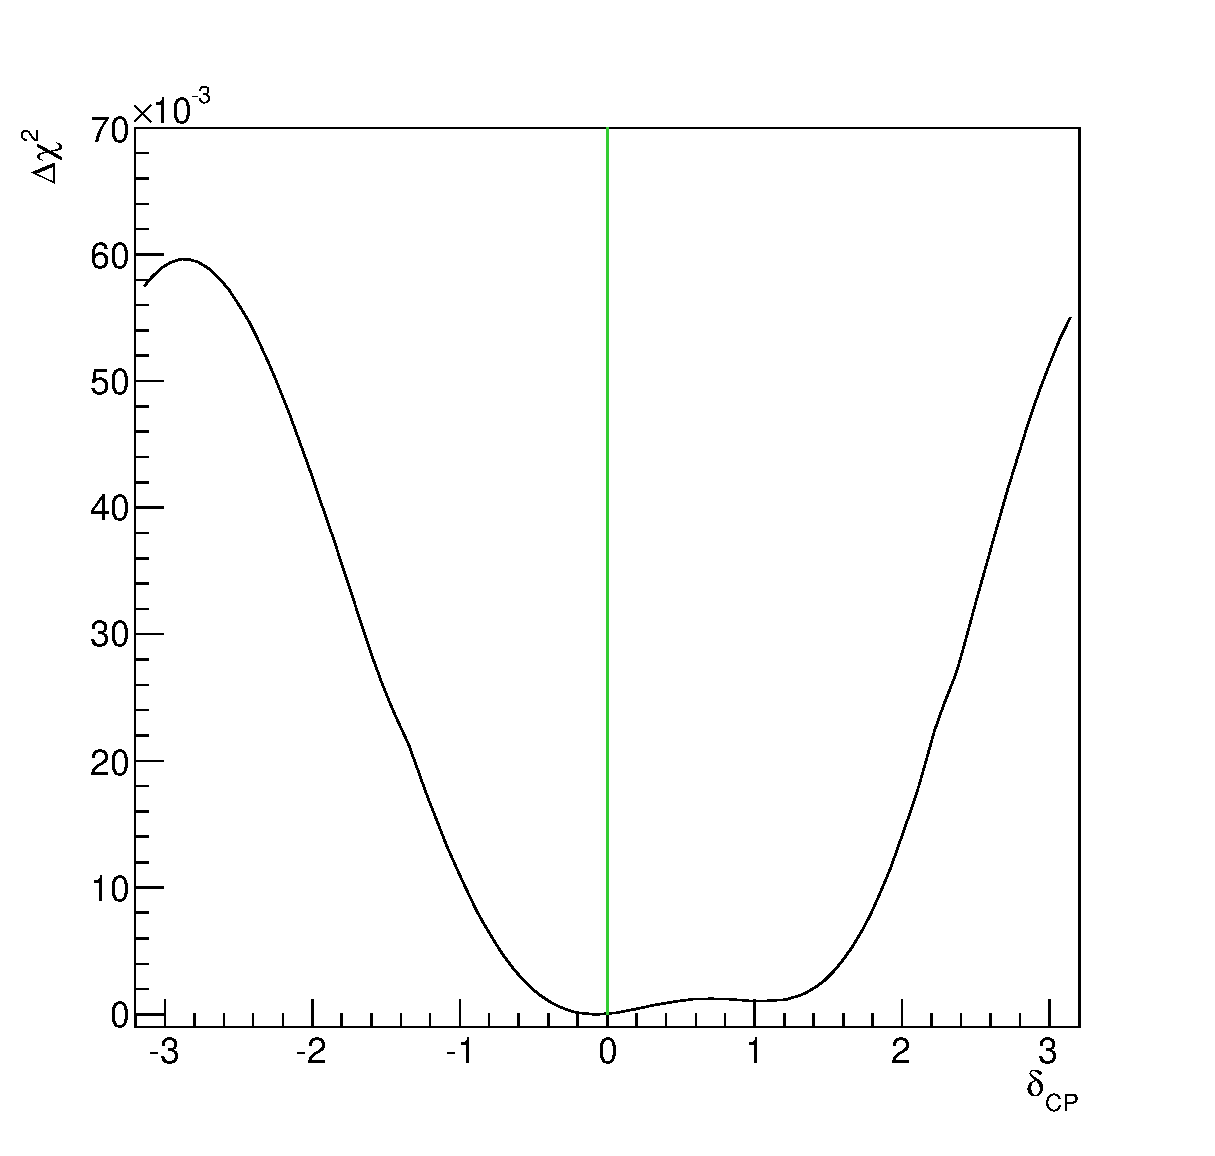
\includegraphics[width=9pc]{.//images/appendix/fake_dataset_fits/fake_dataset0_chisq_deltacp_global_min_new.eps}
\caption {
  $\Delta\chi^2$ as function of $\delta_{CP}$ for fake dataset \#0.
  At each point, $\chi^2$ was minimized with respect to 
  all oscillation parameters not shown (and not considered to be fixed)
  and all relevant nuisance parameters.
}
\label{fig:toymc0_dchisq_deltacp}
\end{minipage}

\vfill
\vspace*{0.7cm}

\begin{minipage}[t]{0.48\linewidth}
\center
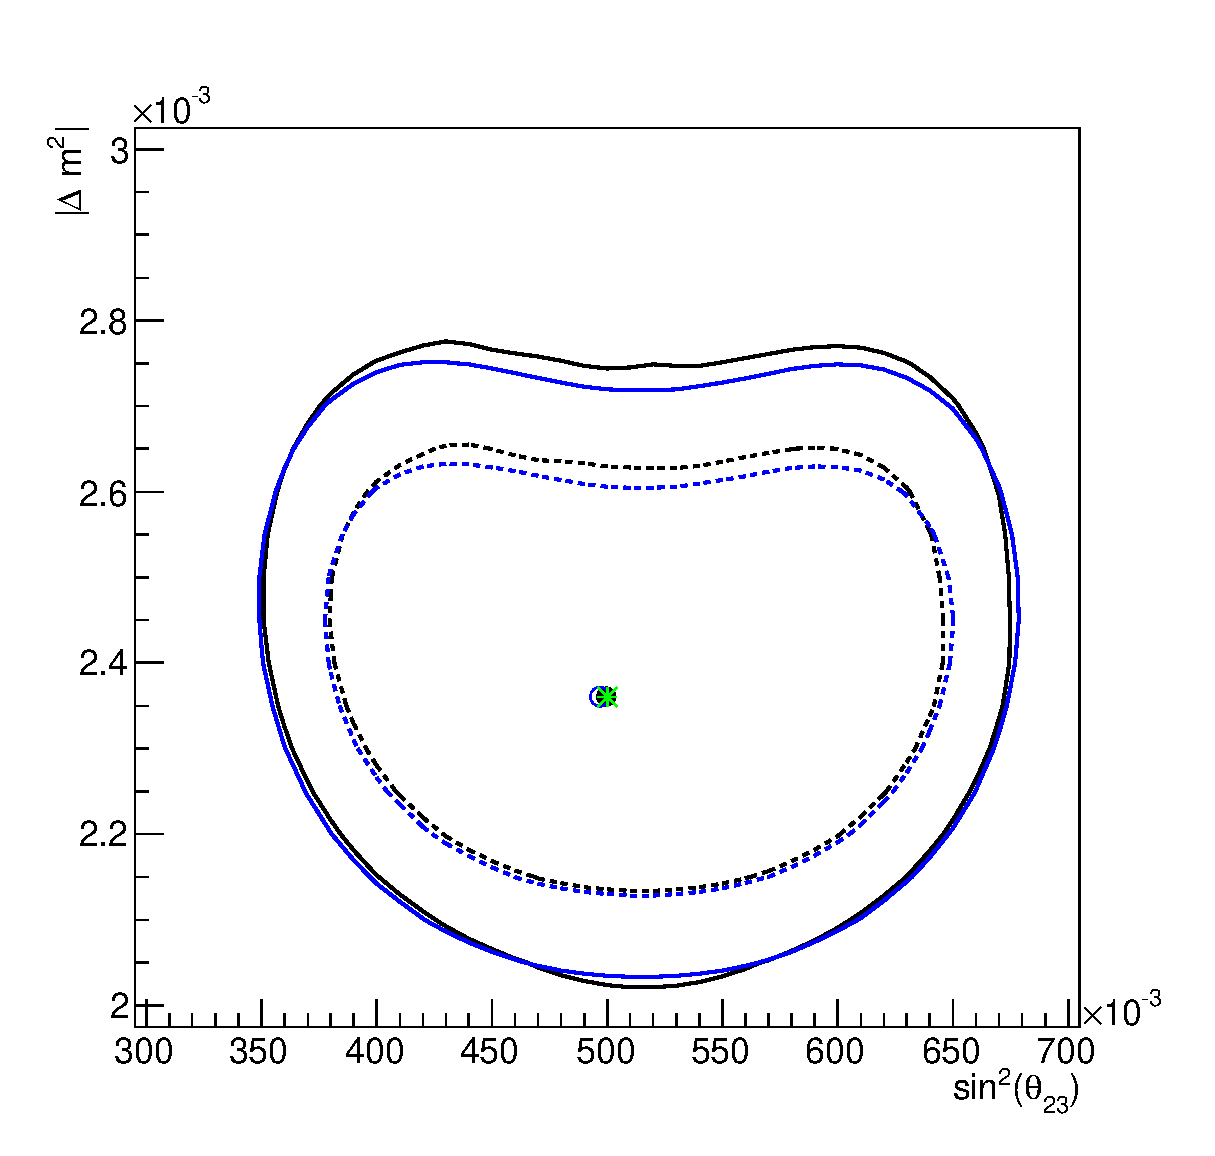
\includegraphics[width=15pc]{./images/appendix/fake_dataset_fits/fake_dataset0_chisq_theta23_dm23sq_global_min_new.eps}
\caption {
  68\% and 90\% CL regions in ($sin^{2}\theta_{23}$, $|\Delta m^{2}|$) space for fake dataset \#0.
  At each point, $\chi^2$ was minimized with respect to 
  $\sin^{2}\theta_{13}$, $\delta_{CP}$
  and all relevant nuisance parameters for the joint analysis (black)
  and with respect to all relevant nuisance parameters for the disappearance analysis (blue). 
}
\label{fig:toymc0_confreg_sinsqtheta23_Dmsq}
\end{minipage}
\hspace{0.03\linewidth}
\begin{minipage}[t]{0.48\linewidth}
\center
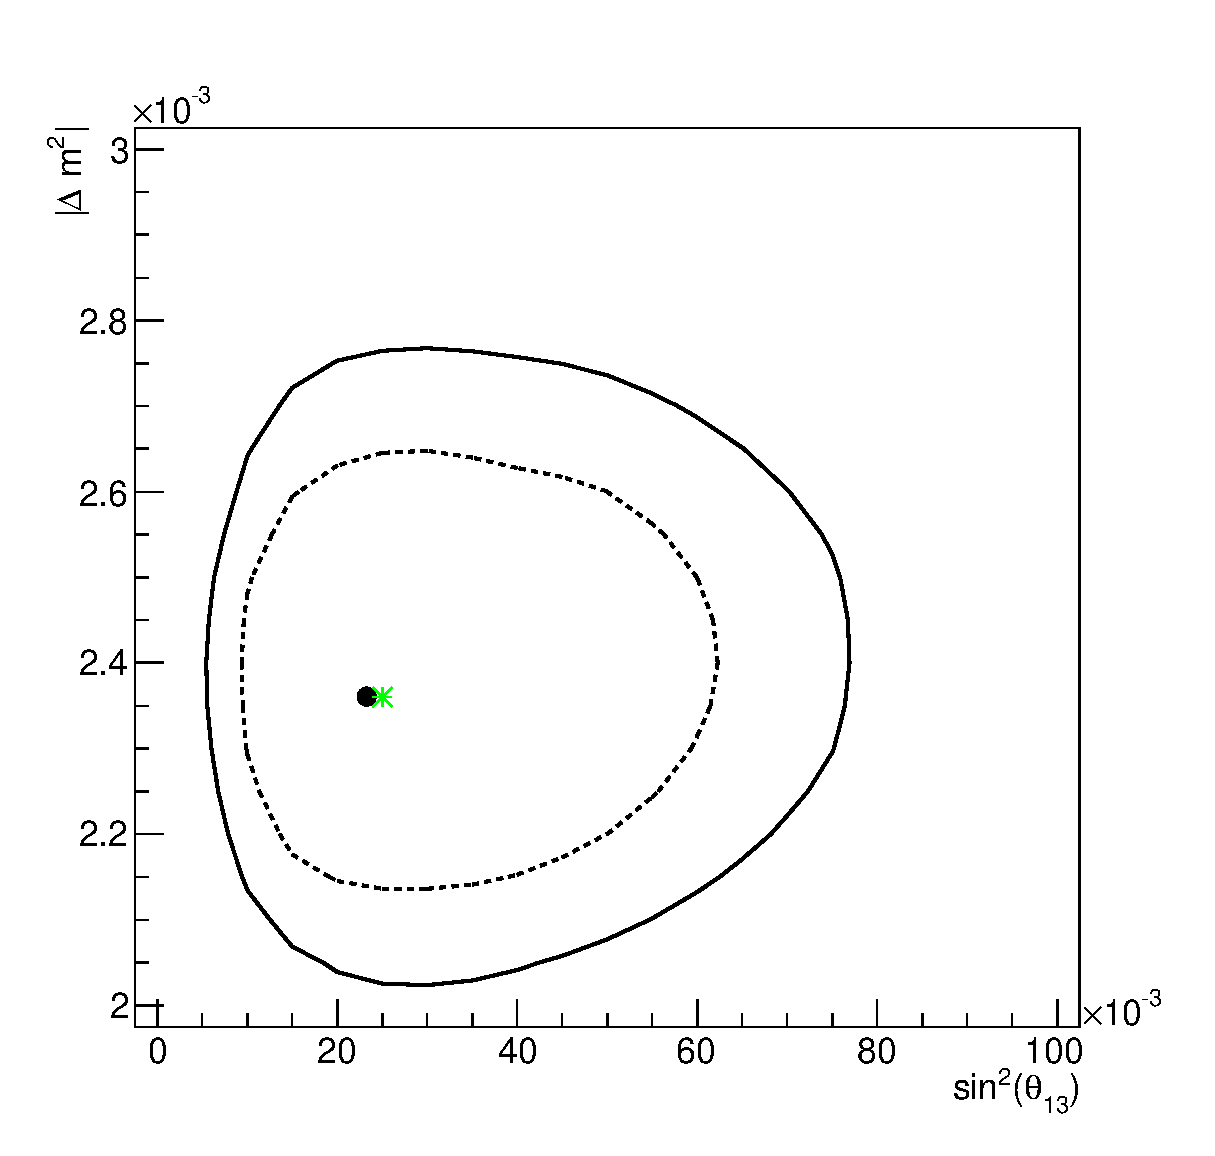
\includegraphics[width=15pc]{./images/appendix/fake_dataset_fits/fake_dataset0_chisq_theta13_dm23sq_global_min_new.eps}
\caption {
  68\% and 90\% CL regions in ($sin^{2}\theta_{13}$, $|\Delta m^{2}|$) space for fake dataset \#0.
  At each point, $\chi^2$ was minimized with respect to 
  all oscillation parameters not shown (and not considered to be fixed)
  and all relevant nuisance parameters.
}
\label{fig:toymc0_confreg_sinsqtheta13_Dmsq}
\end{minipage}

\vfill
\vspace*{0.7cm}

\begin{minipage}[t]{0.48\linewidth}
\center
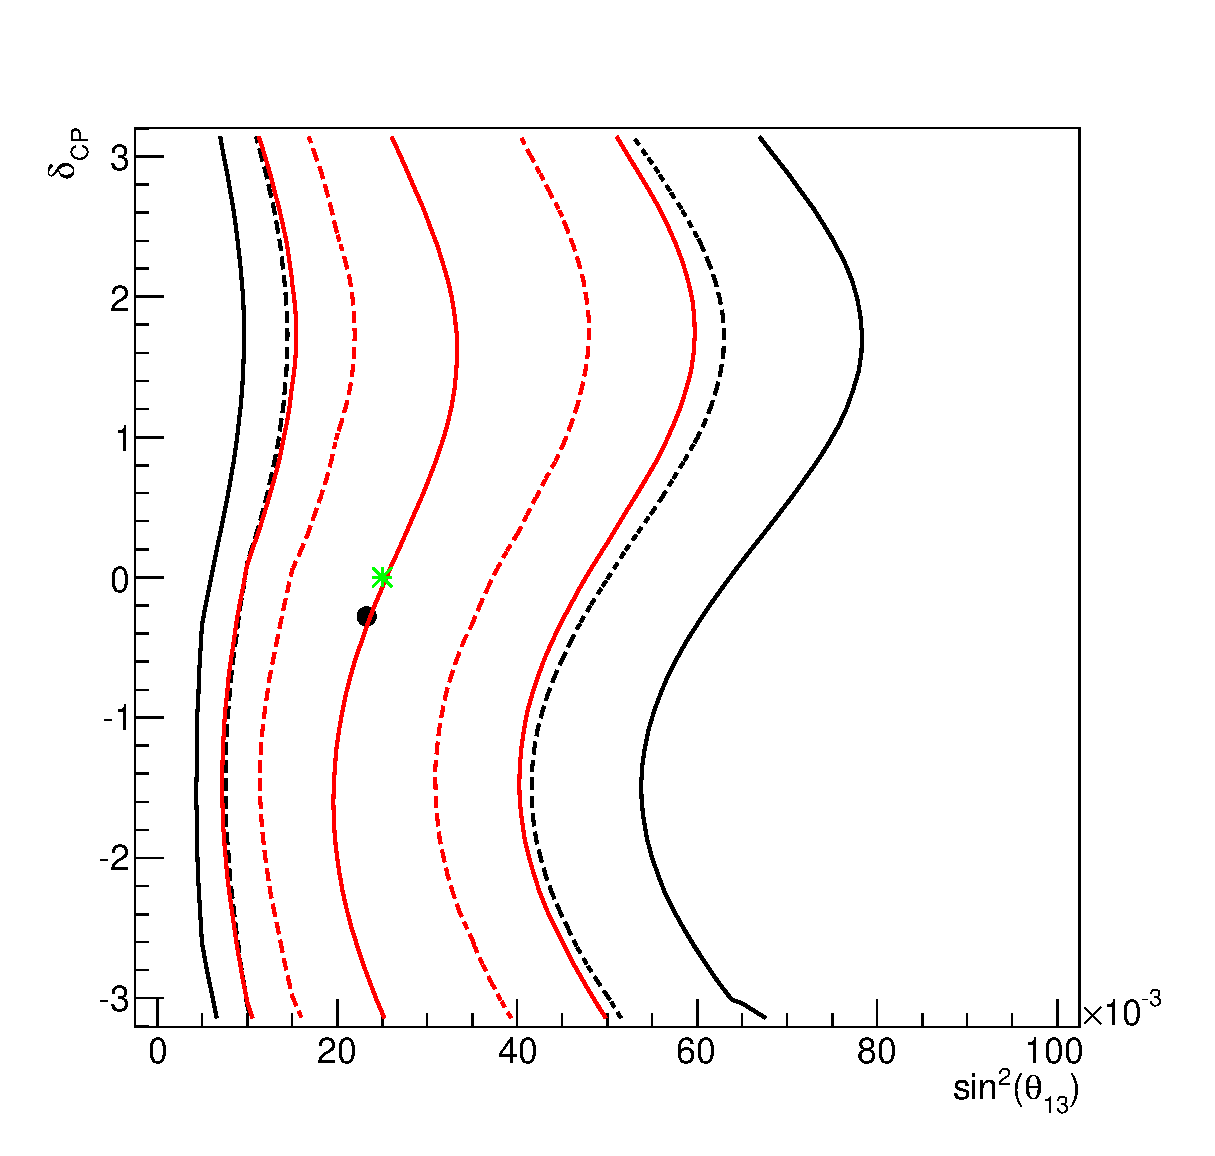
\includegraphics[width=15pc]{./images/appendix/fake_dataset_fits/fake_dataset0_chisq_theta13_deltacp_global_min_new.eps}
\caption {
  68\% and 90\% CL regions in ($sin^{2}\theta_{13}$, $\delta_{CP}$) space for fake dataset \#0.
  At each point, $\chi^2$ was minimized with respect to 
  $|\Delta m^{2}|$, $\sin^{2}\theta_{23}$
  and all relevant nuisance parameters for the joint analysis (black)
  and with respect to all relevant nuisance parameters for the appearance analysis (red).
  Notice that different methods are used to
  construct confidence regions for the joint analysis (global minimum) and for the 
  stand-alone appearance analysis (raster scan).
}
\label{fig:toymc0_confreg_sinsqtheta13_deltacp}
\end{minipage}
\hspace{0.03\linewidth}
\begin{minipage}[t]{0.48\linewidth}
\center
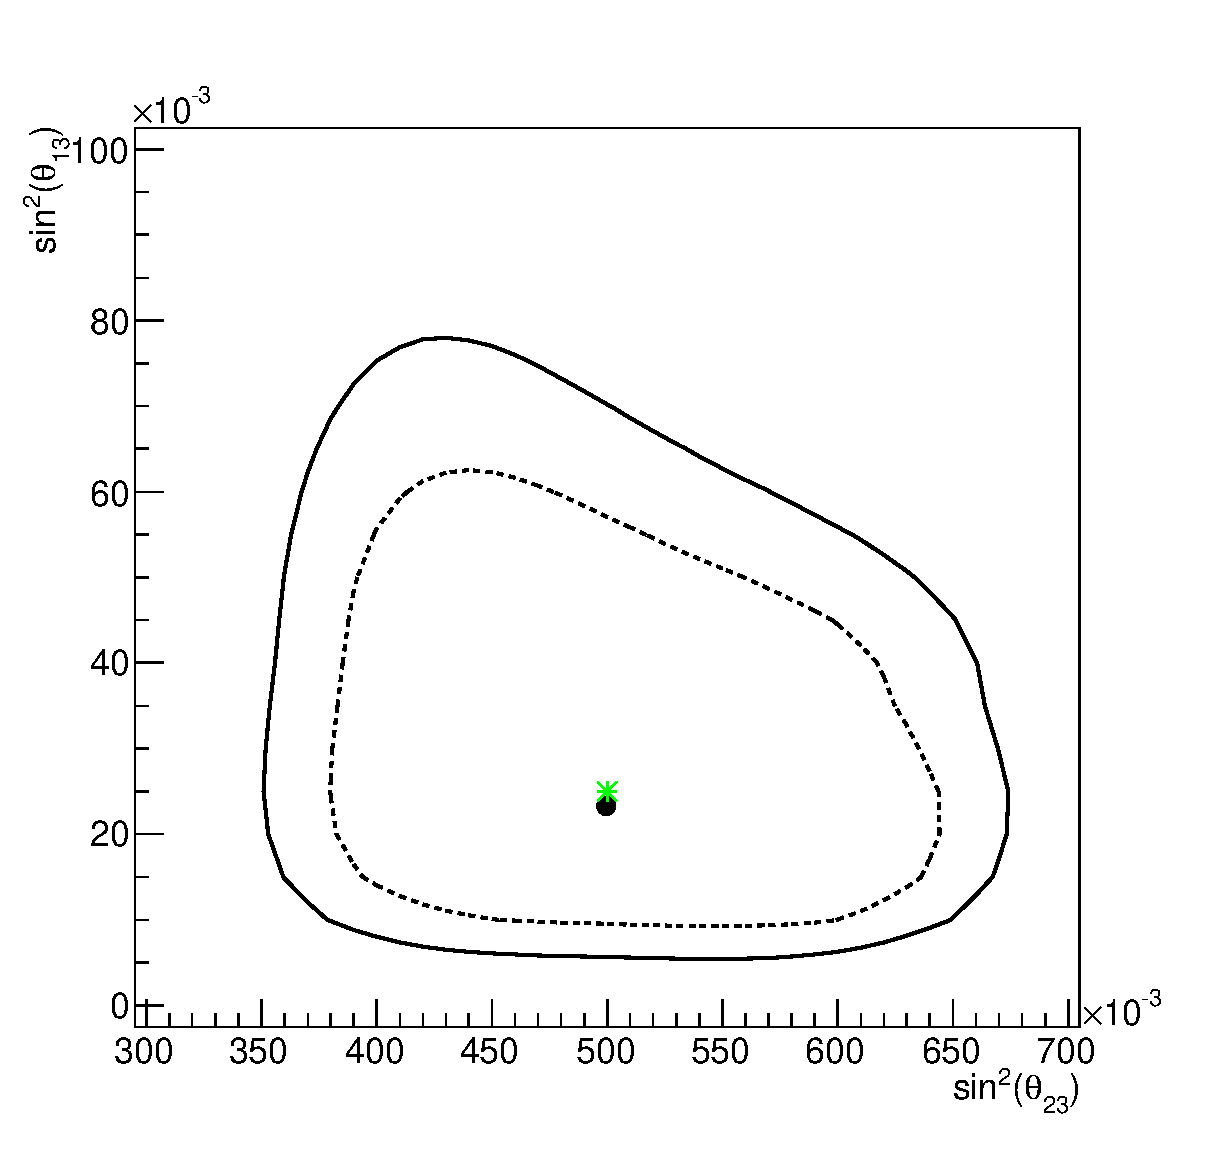
\includegraphics[width=15pc]{./images/appendix/fake_dataset_fits/fake_dataset0_chisq_theta13_theta23_global_min_new.eps}
\caption {
  68\% and 90\% CL regions in ($sin^{2}\theta_{23}$, $sin^{2}\theta_{13}$) space for fake dataset \#0.
  At each point, $\chi^2$ was minimized with respect to 
  all oscillation parameters not shown (and not considered to be fixed)
  and all relevant nuisance parameters.
}
\label{fig:toymc0_confreg_sinsqtheta23_sinsqtheta13}
\end{minipage}

\end{figure*}

\clearpage

%
%
% ..............................................
% Fake dataset #1
%
%


%
% delta\chisq and contours
%

\begin{figure*}[htb]

\begin{minipage}[t]{0.22\linewidth}
\center
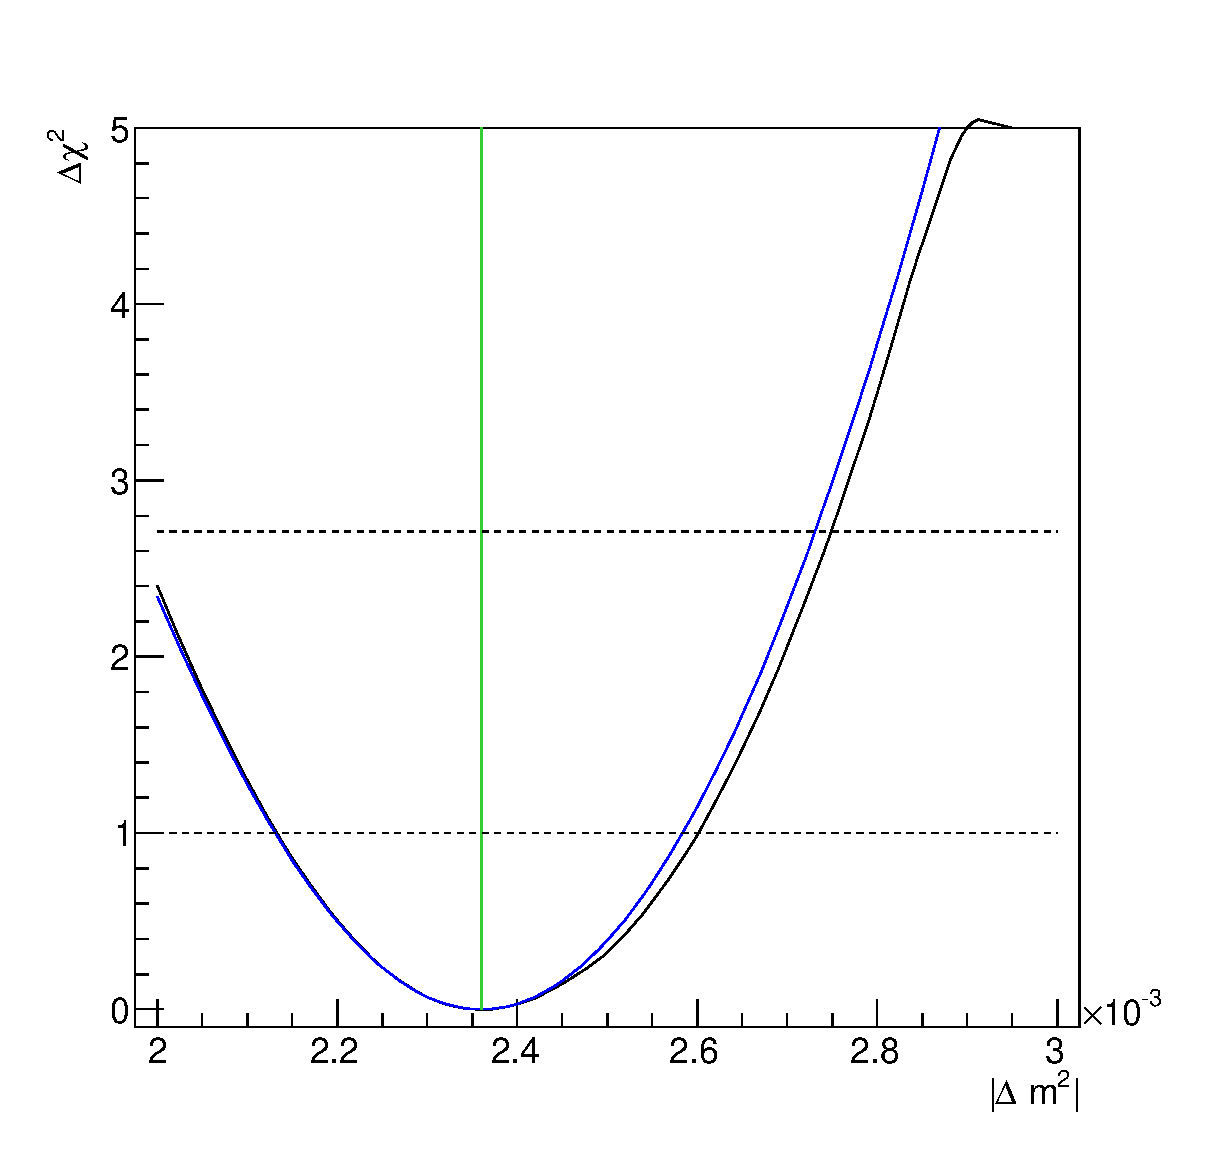
\includegraphics[width=9pc]{./images/appendix/fake_dataset_fits/fake_dataset1_chisq_dm23sq_global_min_new.eps}
\caption {
  $\Delta\chi^2$ as function of $|\Delta m^{2}|$ for fake dataset \#1.
  At each point, $\chi^2$ was minimized with respect to 
  $\sin^{2}\theta_{23}$, $\sin^{2}\theta_{13}$, $\delta_{CP}$
  and all relevant nuisance parameters for the joint analysis (black)
  and with respect to $\sin^{2}\theta_{23}$ and all relevant nuisance
  parameters for the disappearance analysis (blue).
}
\label{fig:toymc1_dchisq_Dmsq}
\end{minipage}
\hspace{0.02\linewidth}
\begin{minipage}[t]{0.22\linewidth}
\center
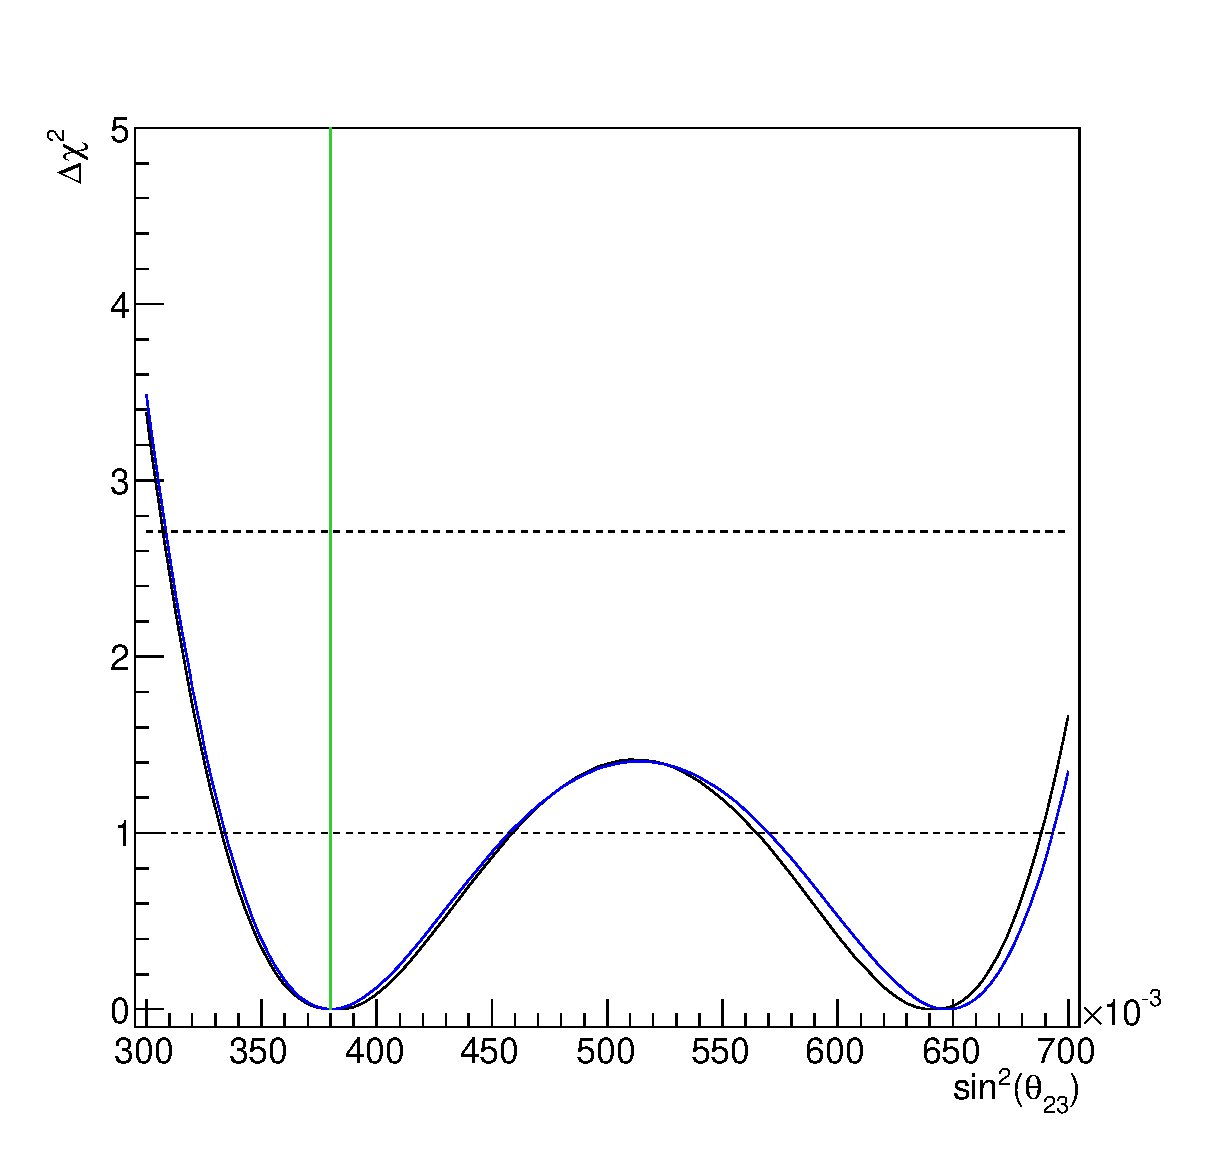
\includegraphics[width=9pc]{./images/appendix/fake_dataset_fits/fake_dataset1_chisq_theta23_global_min_new.eps}
\caption {
  $\Delta\chi^2$ as function of $sin^{2}\theta_{23}$ for fake dataset \#1.
  At each point, $\chi^2$ was minimized with respect to 
  $|\Delta m^{2}|$, $\sin^{2}\theta_{13}$, $\delta_{CP}$
  and all relevant nuisance parameters for the joint analysis (black)
  and with respect to $\sin^{2}\theta_{23}$ and all relevant nuisance
  parameters for the disappearance analysis (blue).
}
\label{fig:toymc1_dchisq_sinsqtheta23}
\end{minipage}
\hspace{0.02\linewidth}
\begin{minipage}[t]{0.22\linewidth}
\center
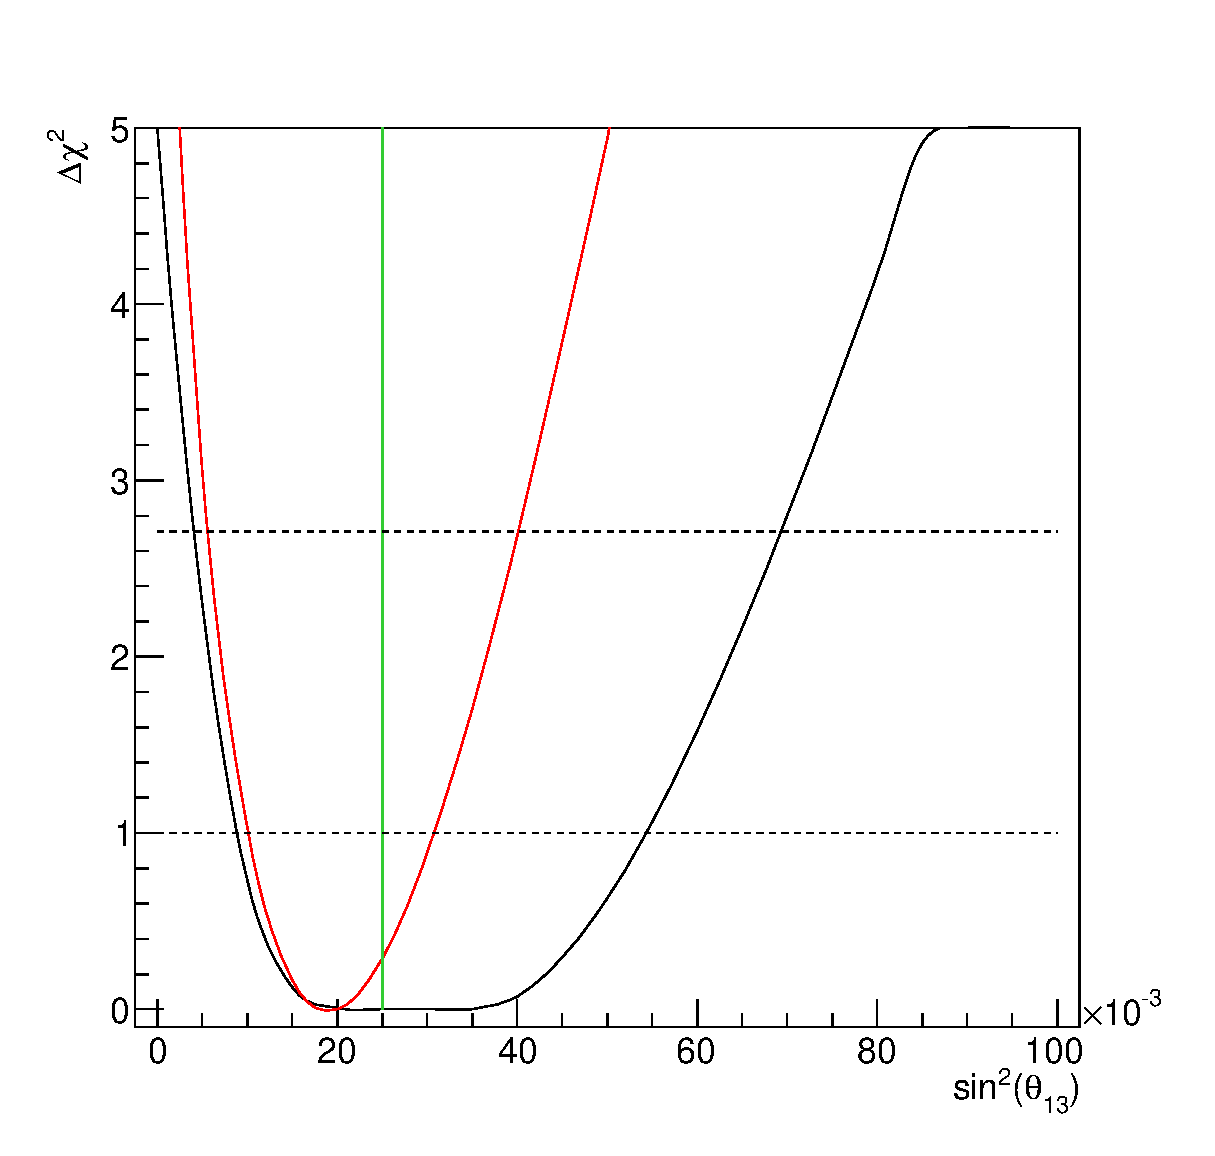
\includegraphics[width=9pc]{./images/appendix/fake_dataset_fits/fake_dataset1_chisq_theta13_global_min_new.eps}
\caption {
  $\Delta\chi^2$ as function of $sin^{2}\theta_{13}$ for fake dataset \#1.
  At each point, $\chi^2$ was minimized with respect to 
  $\sin^{2}\theta_{23}$, $\sin^{2}\theta_{13}$, $\delta_{CP}$
  and all relevant nuisance parameters for the joint analysis (black)
  and with respect to all relevant nuisance parameters 
  ($\delta_{CP}$ is fixed to 0) for the appearance analysis (red).
}
\label{fig:toymc1_dchisq_sinsqtheta13}
\end{minipage}
\hspace{0.02\linewidth}
\begin{minipage}[t]{0.22\linewidth}
\center
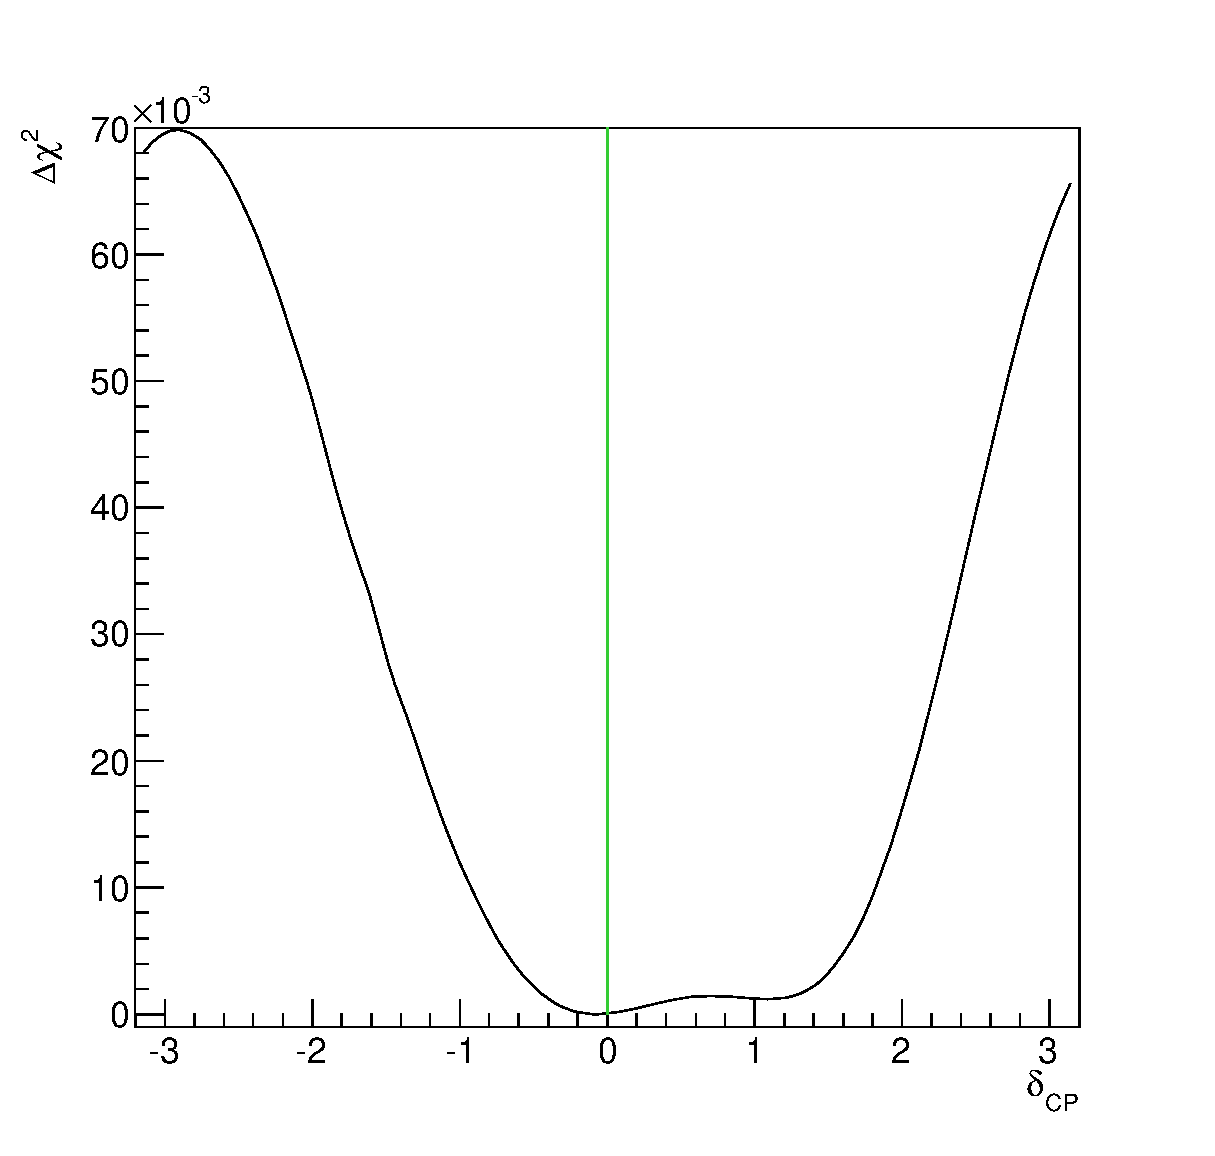
\includegraphics[width=9pc]{.//images/appendix/fake_dataset_fits/fake_dataset1_chisq_deltacp_global_min_new.eps}
\caption {
  $\Delta\chi^2$ as function of $\delta_{CP}$ for fake dataset \#1.
  At each point, $\chi^2$ was minimized with respect to 
  all oscillation parameters not shown (and not considered to be fixed)
  and all relevant nuisance parameters.
}
\label{fig:toymc1_dchisq_deltacp}
\end{minipage}

\vfill
\vspace*{0.7cm}

\begin{minipage}[t]{0.48\linewidth}
\center
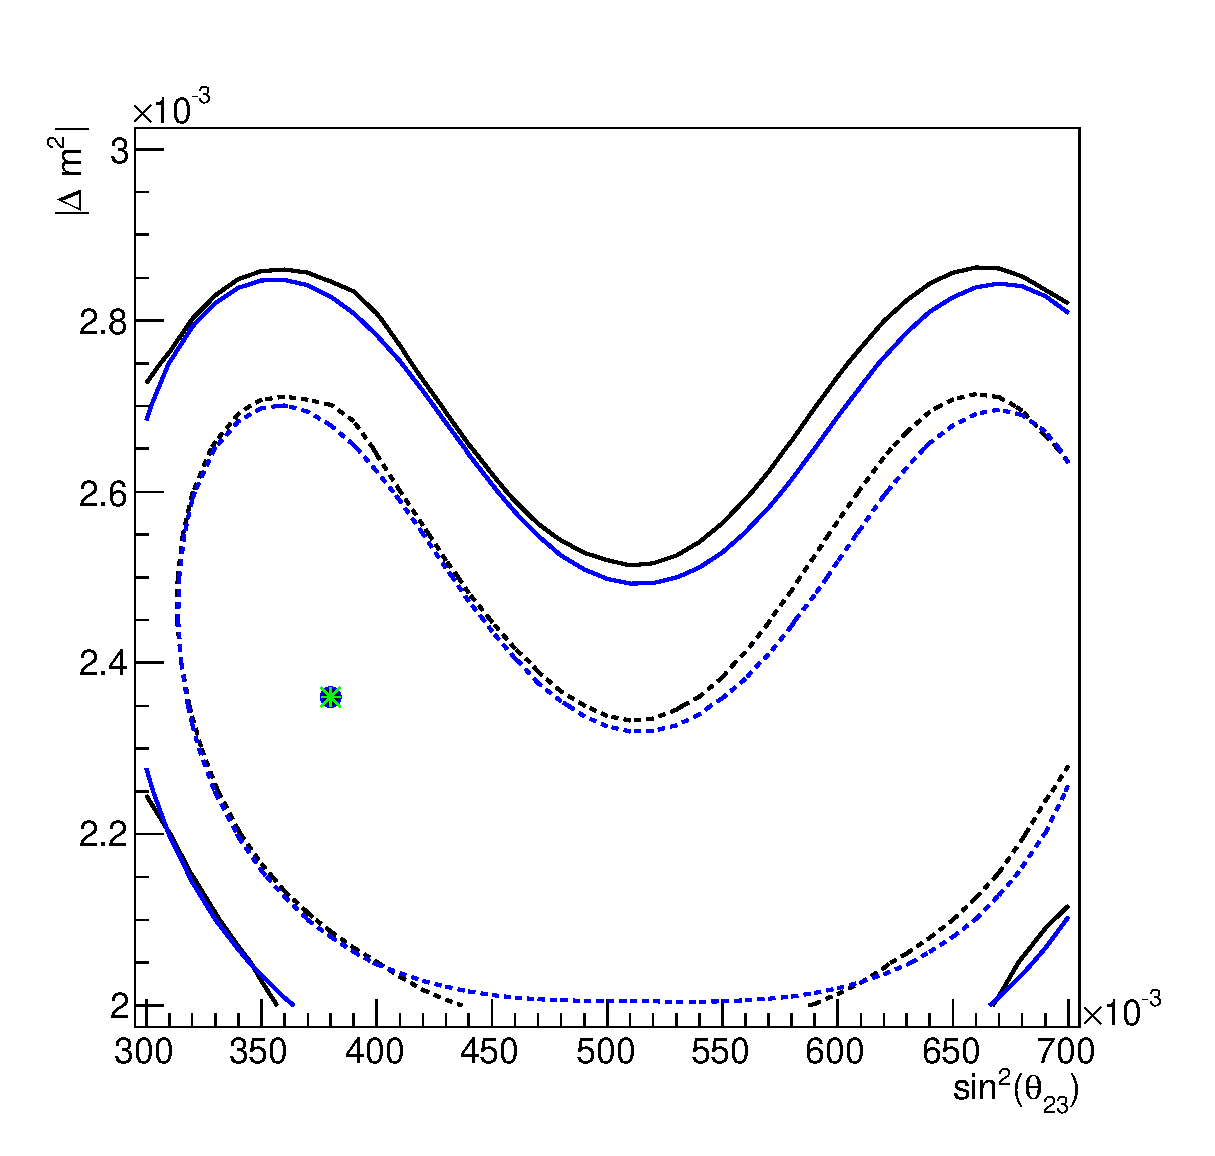
\includegraphics[width=15pc]{./images/appendix/fake_dataset_fits/fake_dataset1_chisq_theta23_dm23sq_global_min_new.eps}
\caption {
  68\% and 90\% CL regions in ($sin^{2}\theta_{23}$, $|\Delta m^{2}|$) space for fake dataset \#1.
  At each point, $\chi^2$ was minimized with respect to 
  $\sin^{2}\theta_{13}$, $\delta_{CP}$
  and all relevant nuisance parameters for the joint analysis (black)
  and with respect to all relevant nuisance parameters for the disappearance analysis (blue).
  }
\label{fig:toymc1_confreg_sinsqtheta23_Dmsq}
\end{minipage}
\hspace{0.03\linewidth}
\begin{minipage}[t]{0.48\linewidth}
\center
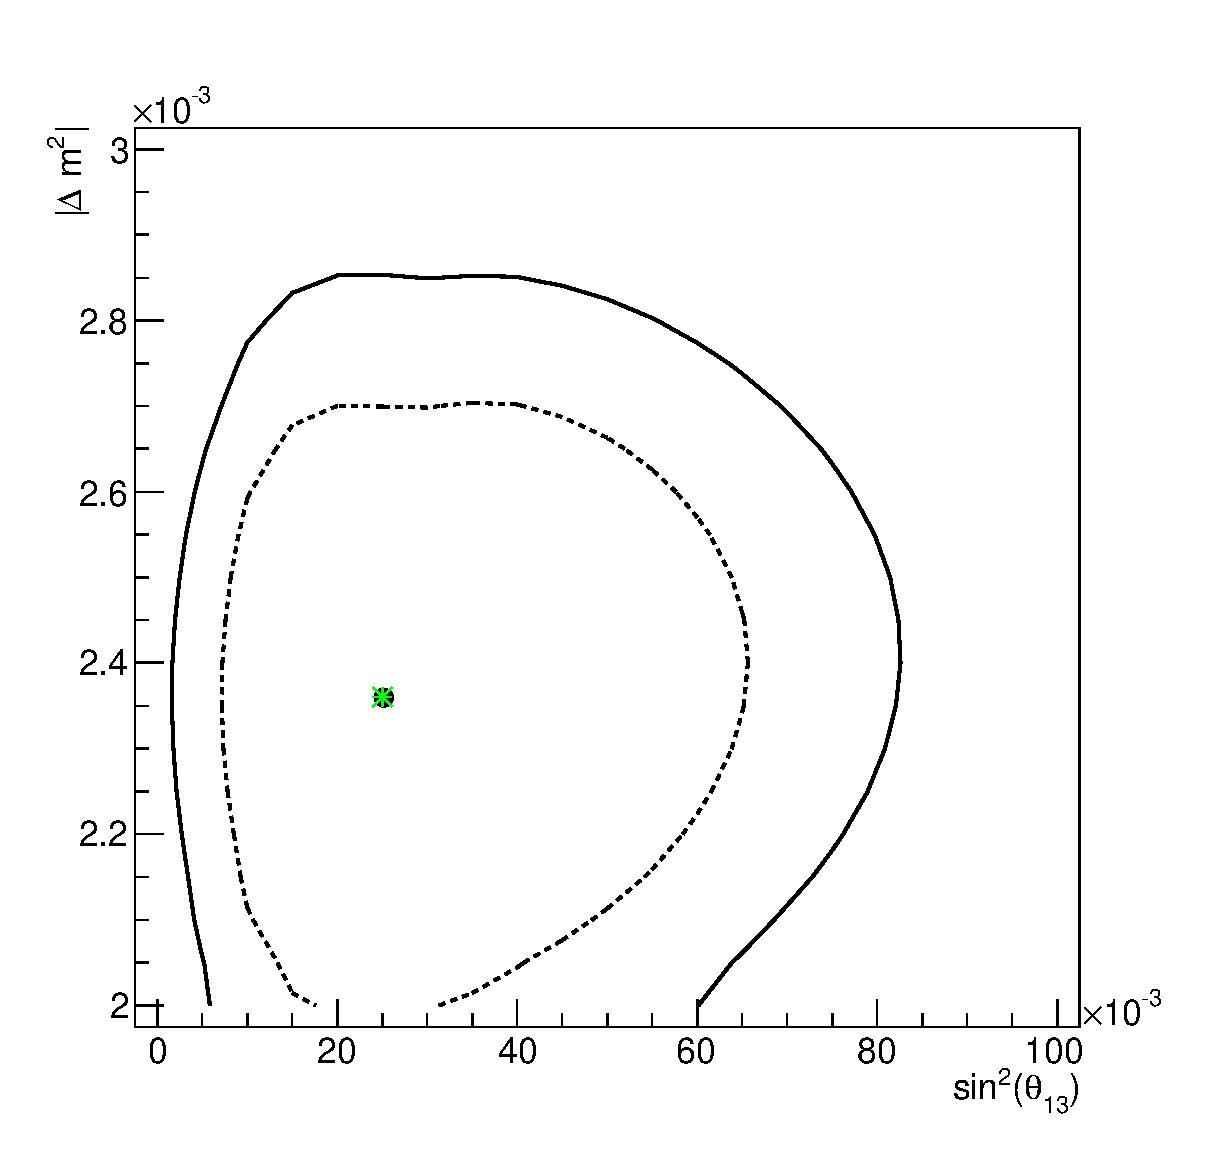
\includegraphics[width=15pc]{./images/appendix/fake_dataset_fits/fake_dataset1_chisq_theta13_dm23sq_global_min_new.eps}
\caption {
  68\% and 90\% CL regions in ($sin^{2}\theta_{13}$, $|\Delta m^{2}|$) space for fake dataset \#1.
  At each point, $\chi^2$ was minimized with respect to 
  all oscillation parameters not shown (and not considered to be fixed)
  and all relevant nuisance parameters.
}
\label{fig:toymc1_confreg_sinsqtheta13_Dmsq}
\end{minipage}

\vfill
\vspace*{0.7cm}

\begin{minipage}[t]{0.48\linewidth}
\center
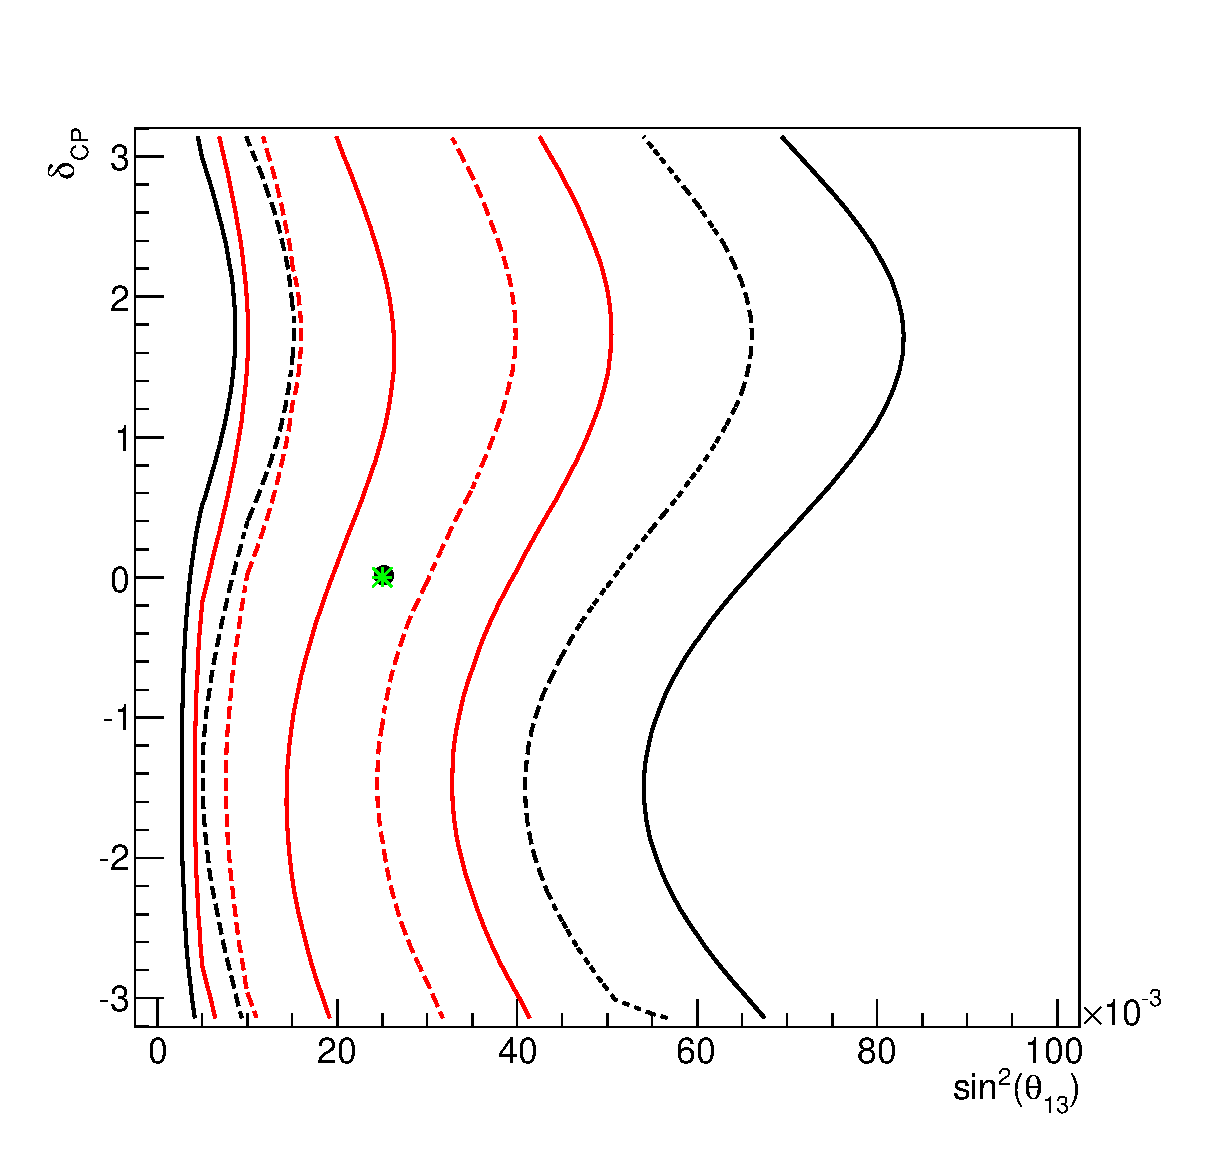
\includegraphics[width=15pc]{./images/appendix/fake_dataset_fits/fake_dataset1_chisq_theta13_deltacp_global_min_new.eps}
\caption {
  68\% and 90\% CL regions in ($sin^{2}\theta_{13}$, $\delta_{CP}$) space for fake dataset \#1.
  At each point, $\chi^2$ was minimized with respect to 
  $|\Delta m^{2}|$, $\sin^{2}\theta_{23}$
  and all relevant nuisance parameters for the joint analysis (black)
  and with respect to all relevant nuisance parameters for the appearance analysis (red).
  Notice that different methods are used to
  construct confidence regions for the joint analysis (global minimum) and for the 
  stand-alone appearance analysis (raster scan).
}
\label{fig:toymc1_confreg_sinsqtheta13_deltacp}
\end{minipage}
\hspace{0.03\linewidth}
\begin{minipage}[t]{0.48\linewidth}
\center
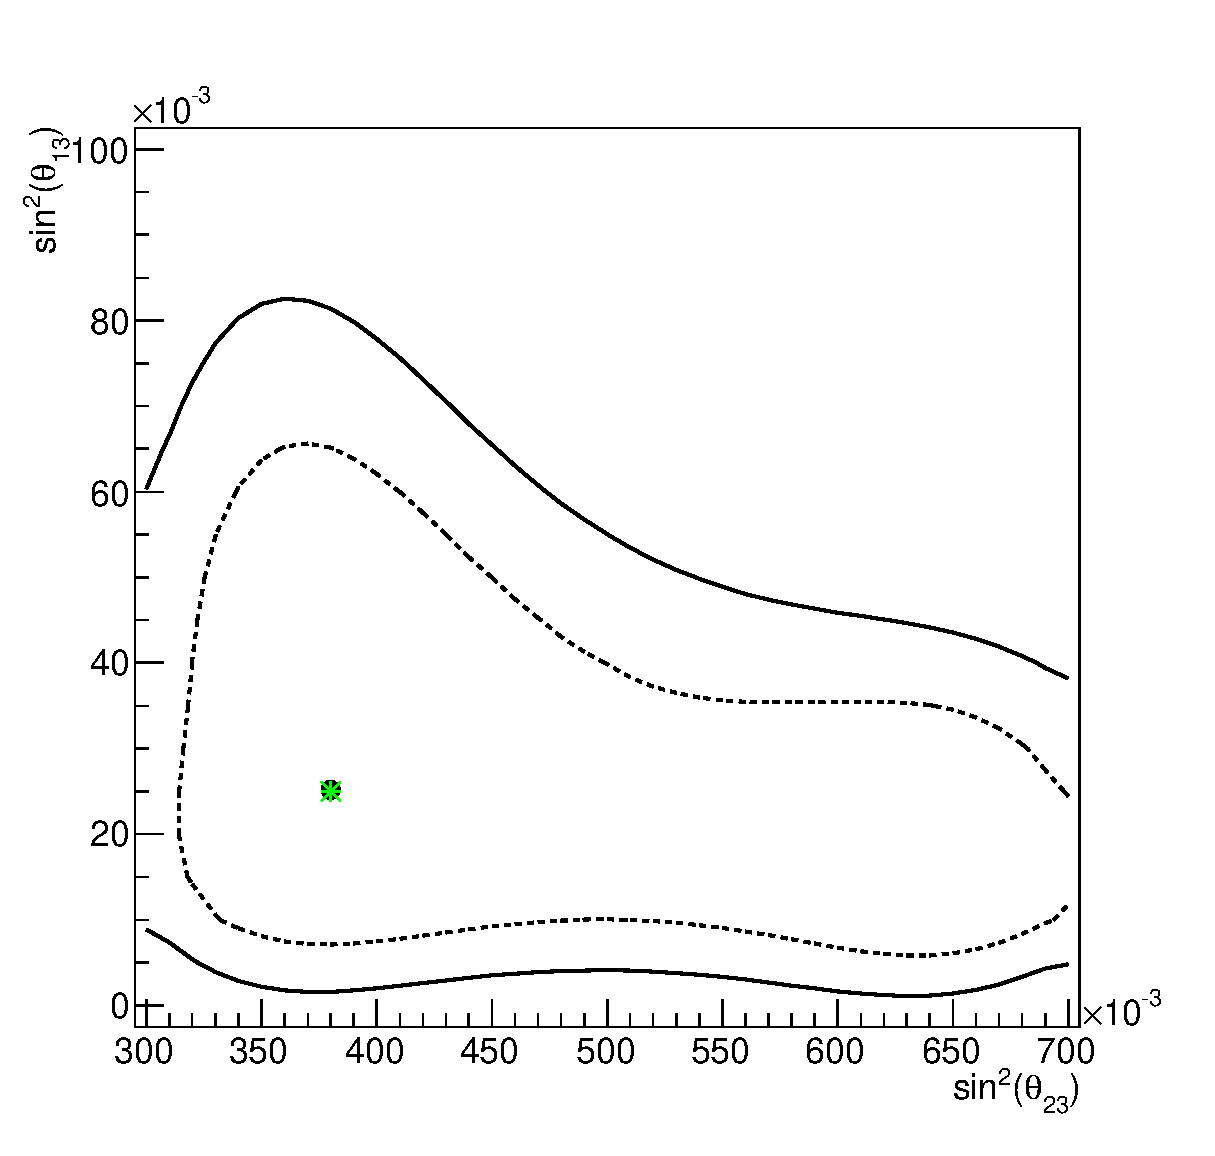
\includegraphics[width=15pc]{./images/appendix/fake_dataset_fits/fake_dataset1_chisq_theta13_theta23_global_min_new.eps}
\caption {
  68\% and 90\% CL regions in ($sin^{2}\theta_{23}$, $sin^{2}\theta_{13}$) space for fake dataset \#1.
  At each point, $\chi^2$ was minimized with respect to 
  all oscillation parameters not shown (and not considered to be fixed)
  and all relevant nuisance parameters.
}
\label{fig:toymc1_confreg_sinsqtheta23_sinsqtheta13}
\end{minipage}

\end{figure*}

%
%
% ..............................................
% Fake dataset #2
%
%

\clearpage

%
% delta\chisq and contours
%

\begin{figure*}[htb]

\begin{minipage}[t]{0.22\linewidth}
\center
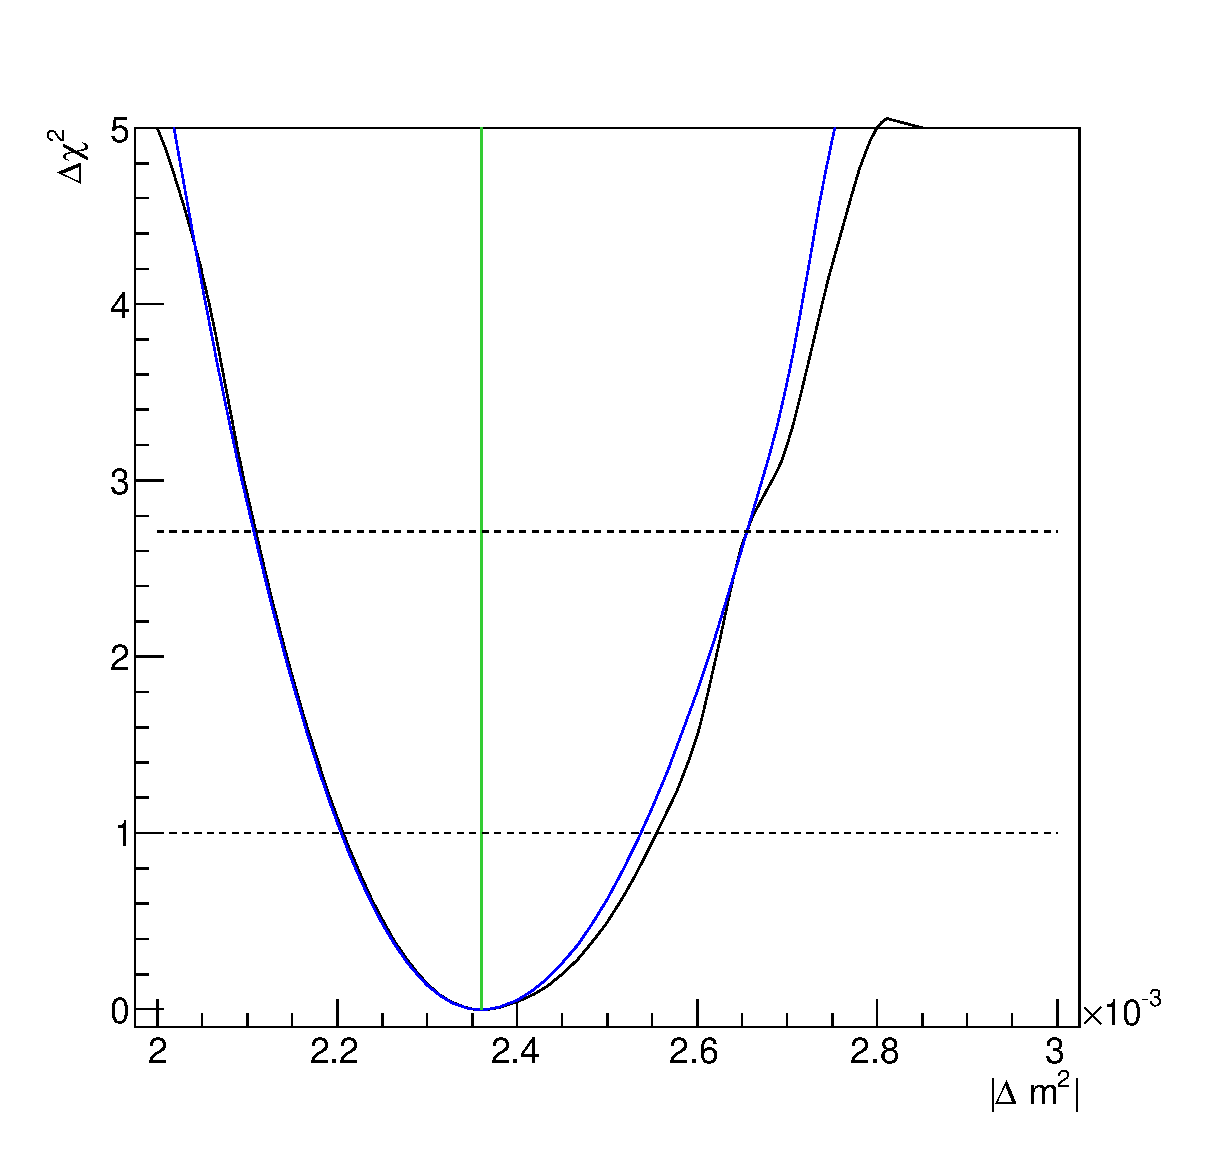
\includegraphics[width=9pc]{./images/appendix/fake_dataset_fits/fake_dataset3_chisq_dm23sq_global_min_new.eps}
\caption {
  $\Delta\chi^2$ as function of $|\Delta m^{2}|$ for fake dataset \#2.
  At each point, $\chi^2$ was minimized with respect to 
  $\sin^{2}\theta_{23}$, $\sin^{2}\theta_{13}$, $\delta_{CP}$
  and all relevant nuisance parameters for the joint analysis (black)
  and with respect to $\sin^{2}\theta_{23}$ and all relevant nuisance
  parameters for the disappearance analysis (blue).
}
\label{fig:toymc2_dchisq_Dmsq}
\end{minipage}
\hspace{0.02\linewidth}
\begin{minipage}[t]{0.22\linewidth}
\center
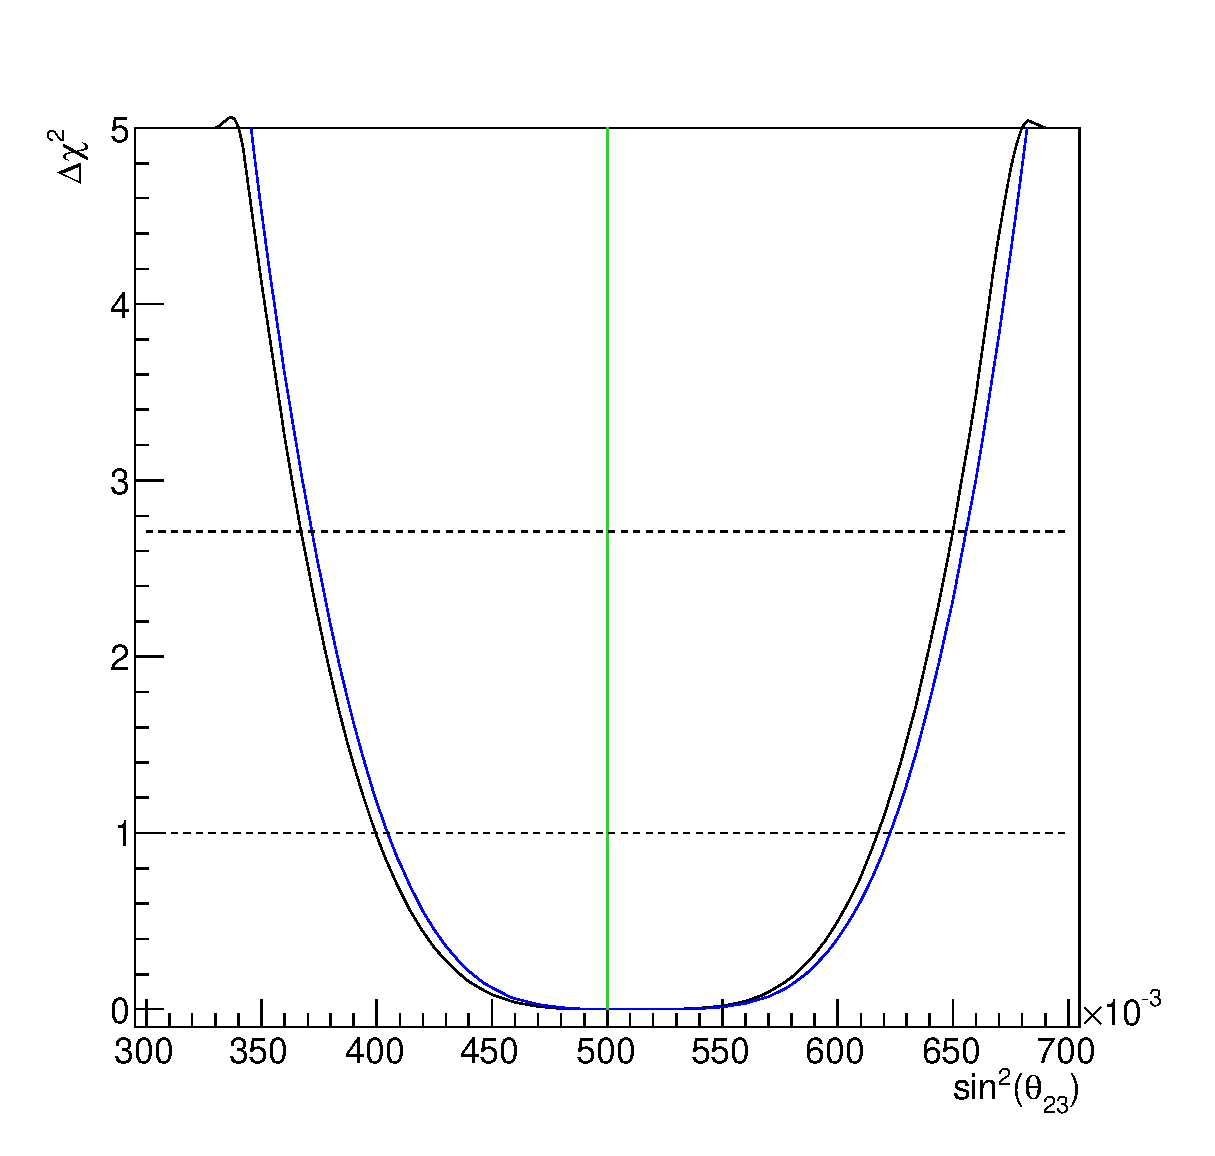
\includegraphics[width=9pc]{./images/appendix/fake_dataset_fits/fake_dataset3_chisq_theta23_global_min_new.eps}
\caption {
  $\Delta\chi^2$ as function of $sin^{2}\theta_{23}$ for fake dataset \#2.
  At each point, $\chi^2$ was minimized with respect to 
  $|\Delta m^{2}|$, $\sin^{2}\theta_{13}$, $\delta_{CP}$
  and all relevant nuisance parameters for the joint analysis (black)
  and with respect to $\sin^{2}\theta_{23}$ and all relevant nuisance
  parameters for the disappearance analysis (blue).
}
\label{fig:toymc2_dchisq_sinsqtheta23}
\end{minipage}
\hspace{0.02\linewidth}
\begin{minipage}[t]{0.22\linewidth}
\center
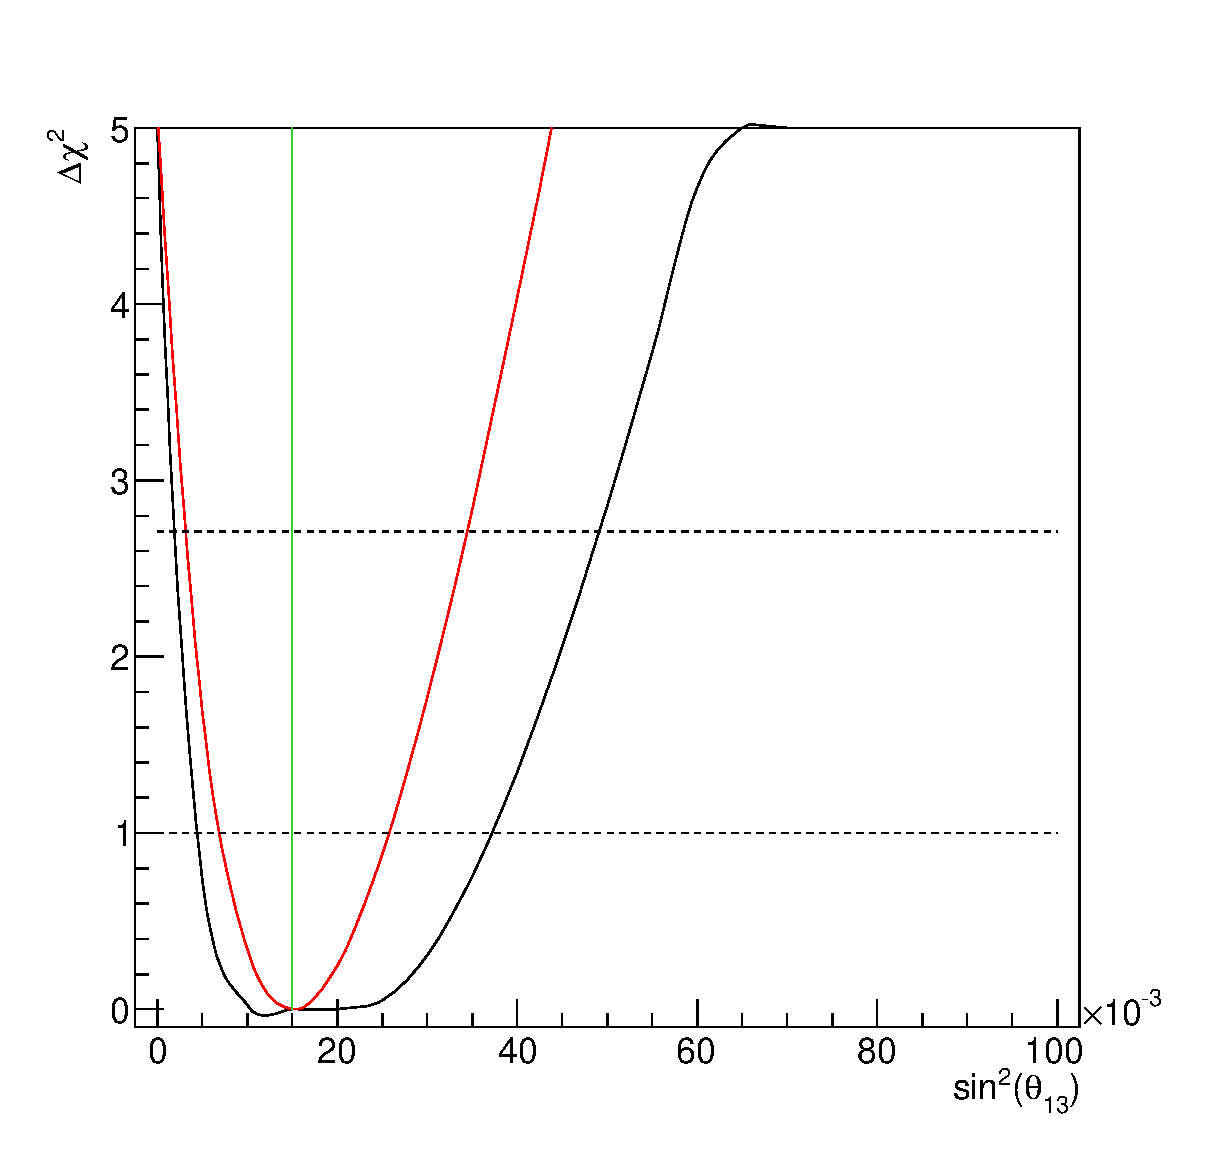
\includegraphics[width=9pc]{./images/appendix/fake_dataset_fits/fake_dataset3_chisq_theta13_global_min_new.eps}
\caption {
  $\Delta\chi^2$ as function of $sin^{2}\theta_{13}$ for fake dataset \#2.
  At each point, $\chi^2$ was minimized with respect to 
  $\sin^{2}\theta_{23}$, $\sin^{2}\theta_{13}$, $\delta_{CP}$
  and all relevant nuisance parameters for the joint analysis (black)
  and with respect to all relevant nuisance parameters 
  ($\delta_{CP}$ is fixed to 0) for the appearance analysis (red).
}
\label{fig:toymc2_dchisq_sinsqtheta13}
\end{minipage}
\hspace{0.02\linewidth}
\begin{minipage}[t]{0.22\linewidth}
\center
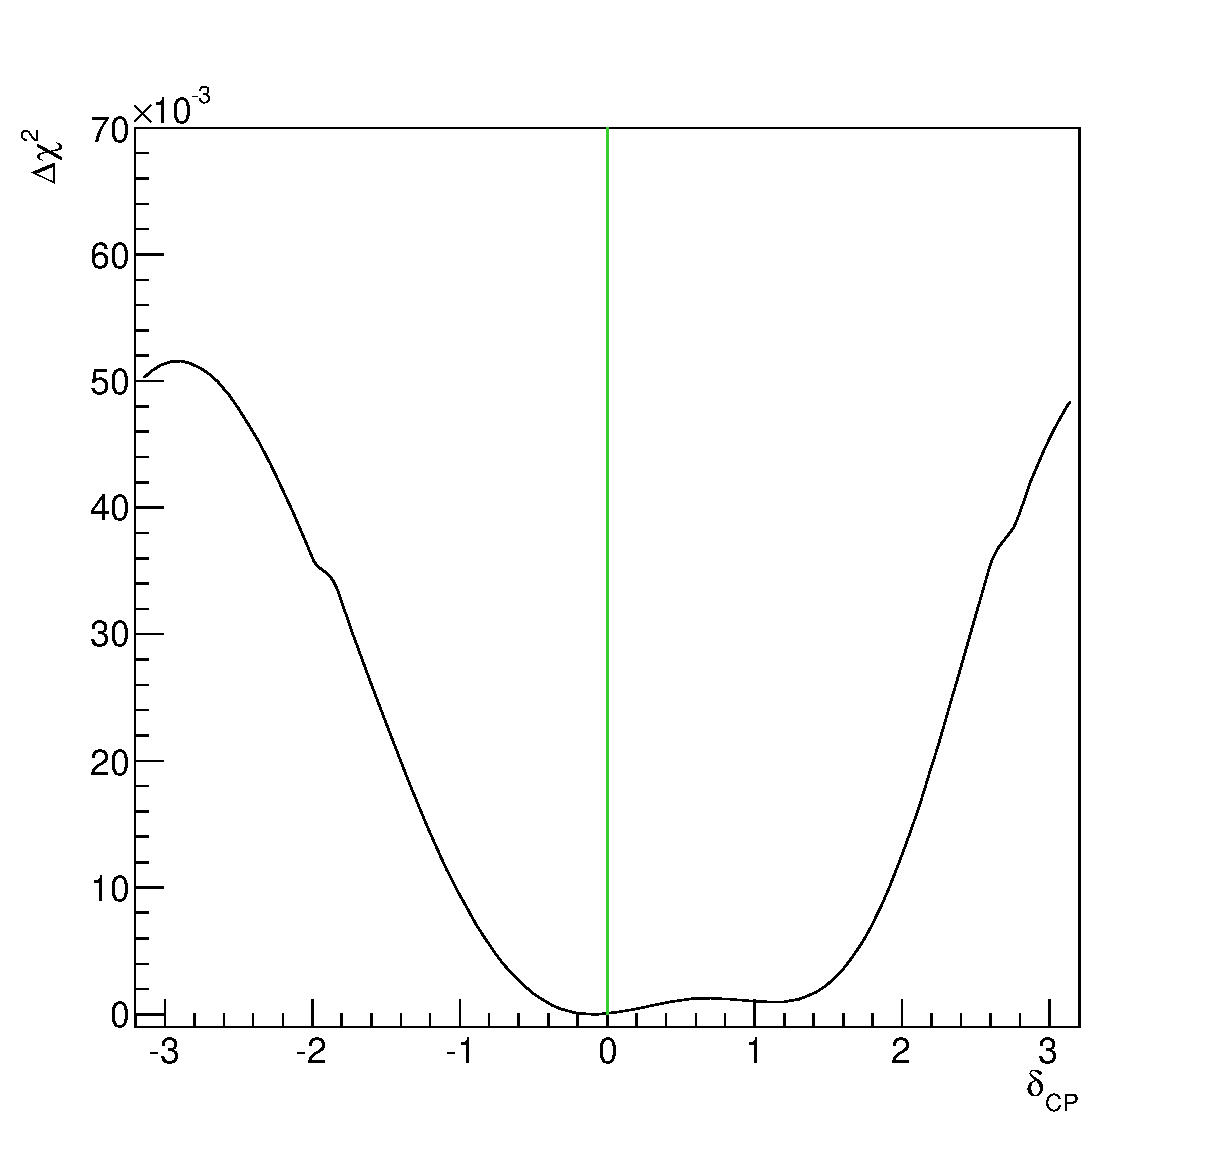
\includegraphics[width=9pc]{.//images/appendix/fake_dataset_fits/fake_dataset3_chisq_deltacp_global_min_new.eps}
\caption {
  $\Delta\chi^2$ as function of $\delta_{CP}$ for fake dataset \#2.
  At each point, $\chi^2$ was minimized with respect to 
  all oscillation parameters not shown (and not considered to be fixed)
  and all relevant nuisance parameters.
}
\label{fig:toymc2_dchisq_deltacp}
\end{minipage}

\vfill
\vspace*{0.7cm}

\begin{minipage}[t]{0.48\linewidth}
\center
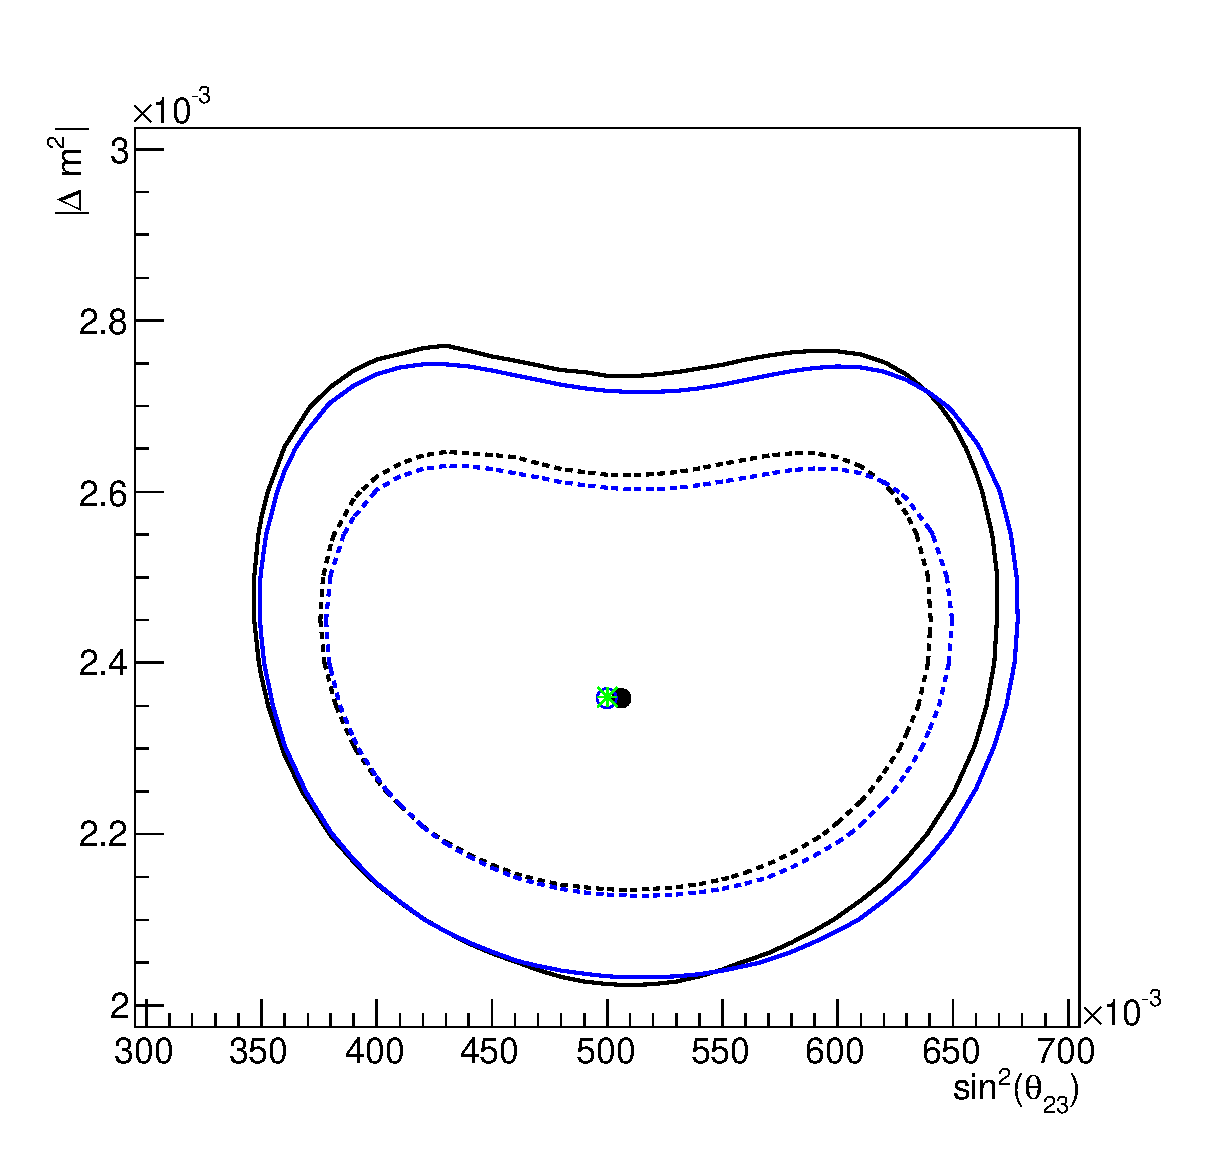
\includegraphics[width=15pc]{./images/appendix/fake_dataset_fits/fake_dataset3_chisq_theta23_dm23sq_global_min_new.eps}
\caption {
  68\% and 90\% CL regions in ($sin^{2}\theta_{23}$, $|\Delta m^{2}|$) space for fake dataset \#2.
  At each point, $\chi^2$ was minimized with respect to 
  $\sin^{2}\theta_{13}$, $\delta_{CP}$
  and all relevant nuisance parameters for the joint analysis (black)
  and with respect to all relevant nuisance parameters for the disappearance analysis (blue).
}
\label{fig:toymc2_confreg_sinsqtheta23_Dmsq}
\end{minipage}
\hspace{0.03\linewidth}
\begin{minipage}[t]{0.48\linewidth}
\center
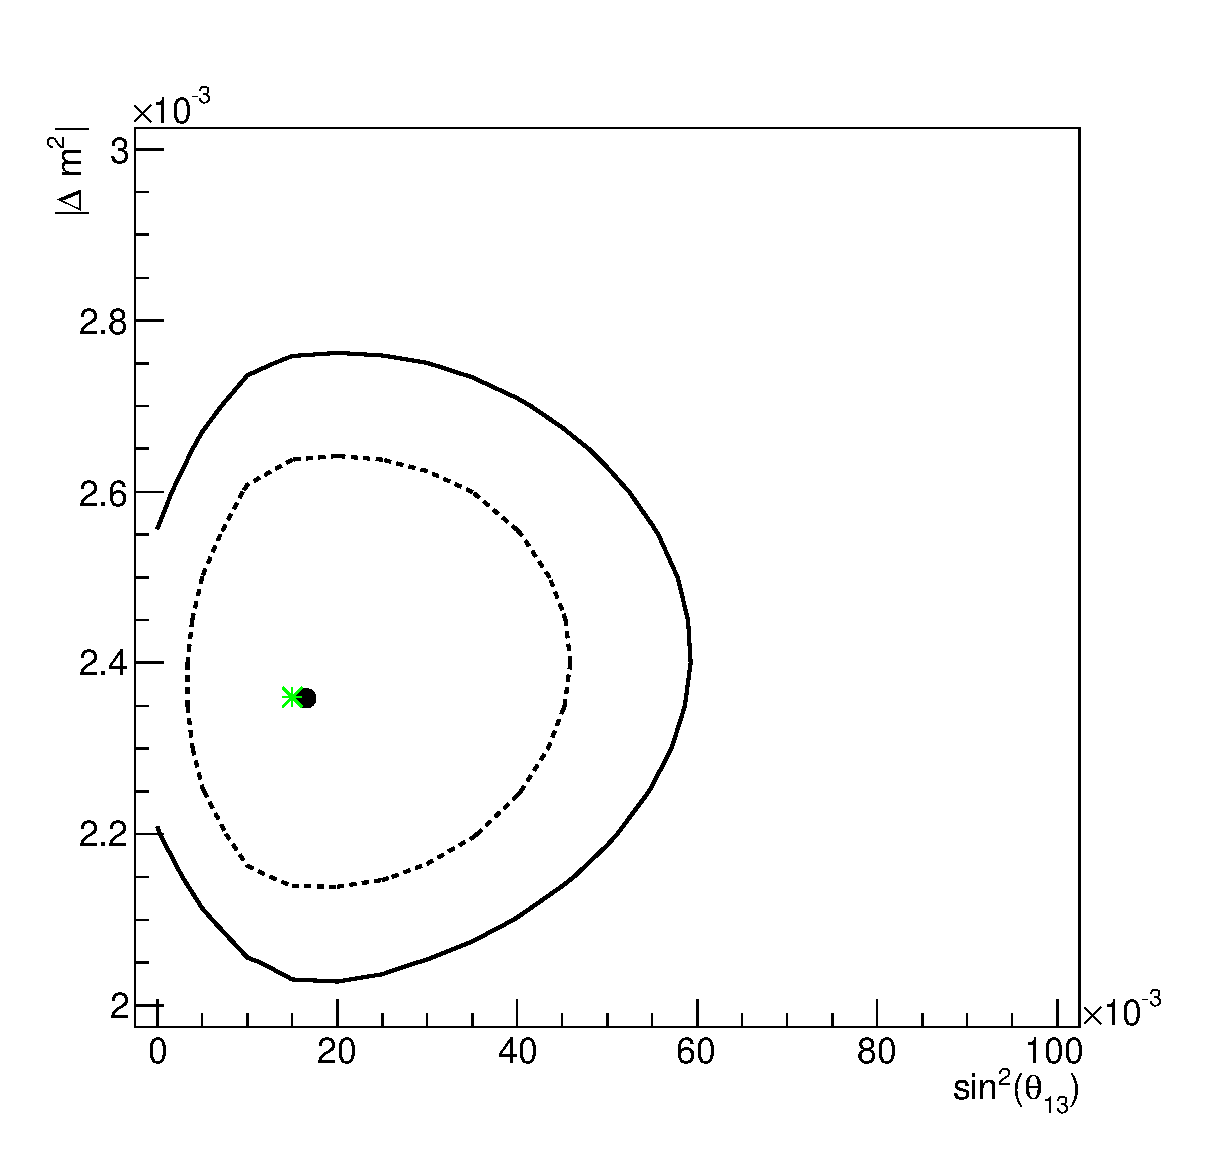
\includegraphics[width=15pc]{./images/appendix/fake_dataset_fits/fake_dataset3_chisq_theta13_dm23sq_global_min_new.eps}
\caption {
  68\% and 90\% CL regions in ($sin^{2}\theta_{13}$, $|\Delta m^{2}|$) space for fake dataset \#2.
  At each point, $\chi^2$ was minimized with respect to 
  all oscillation parameters not shown (and not considered to be fixed)
  and all relevant nuisance parameters.
}
\label{fig:toymc2_confreg_sinsqtheta13_Dmsq}
\end{minipage}

\vfill
\vspace*{0.7cm}

\begin{minipage}[t]{0.48\linewidth}
\center
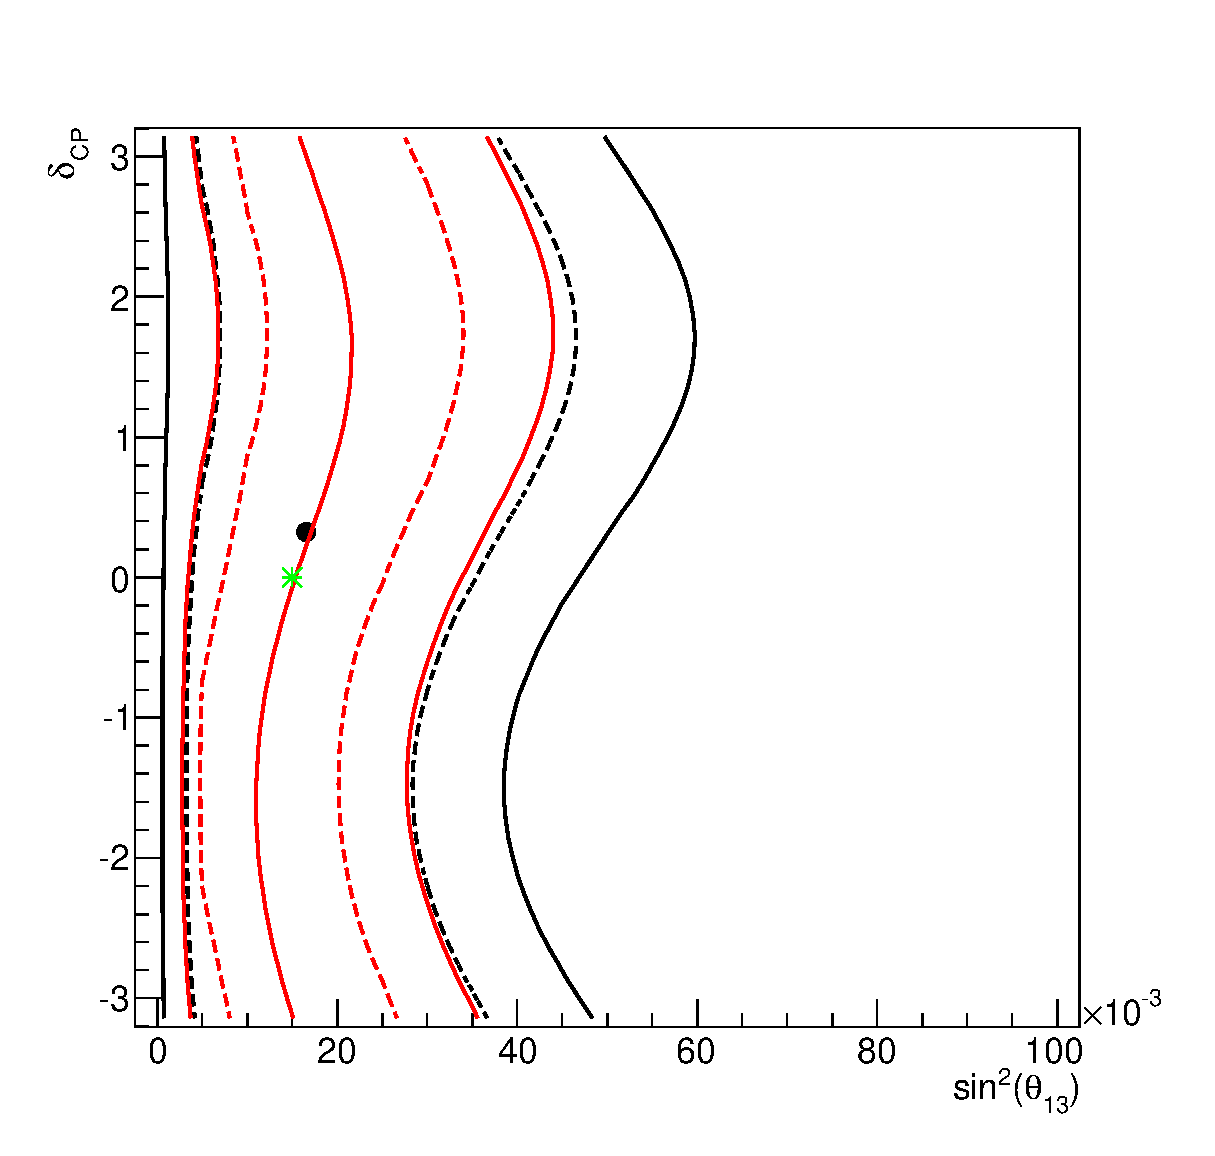
\includegraphics[width=15pc]{./images/appendix/fake_dataset_fits/fake_dataset3_chisq_theta13_deltacp_global_min_new.eps}
\caption {
  68\% and 90\% CL regions in ($sin^{2}\theta_{13}$, $\delta_{CP}$) space for fake dataset \#2.
  At each point, $\chi^2$ was minimized with respect to 
  $|\Delta m^{2}|$, $\sin^{2}\theta_{23}$
  and all relevant nuisance parameters for the joint analysis (black)
  and with respect to all relevant nuisance parameters for the appearance analysis (red).
  Notice that different methods are used to
  construct confidence regions for the joint analysis (global minimum) and for the 
  stand-alone appearance analysis (raster scan).
}
\label{fig:toymc2_confreg_sinsqtheta13_deltacp}
\end{minipage}
\hspace{0.03\linewidth}
\begin{minipage}[t]{0.48\linewidth}
\center
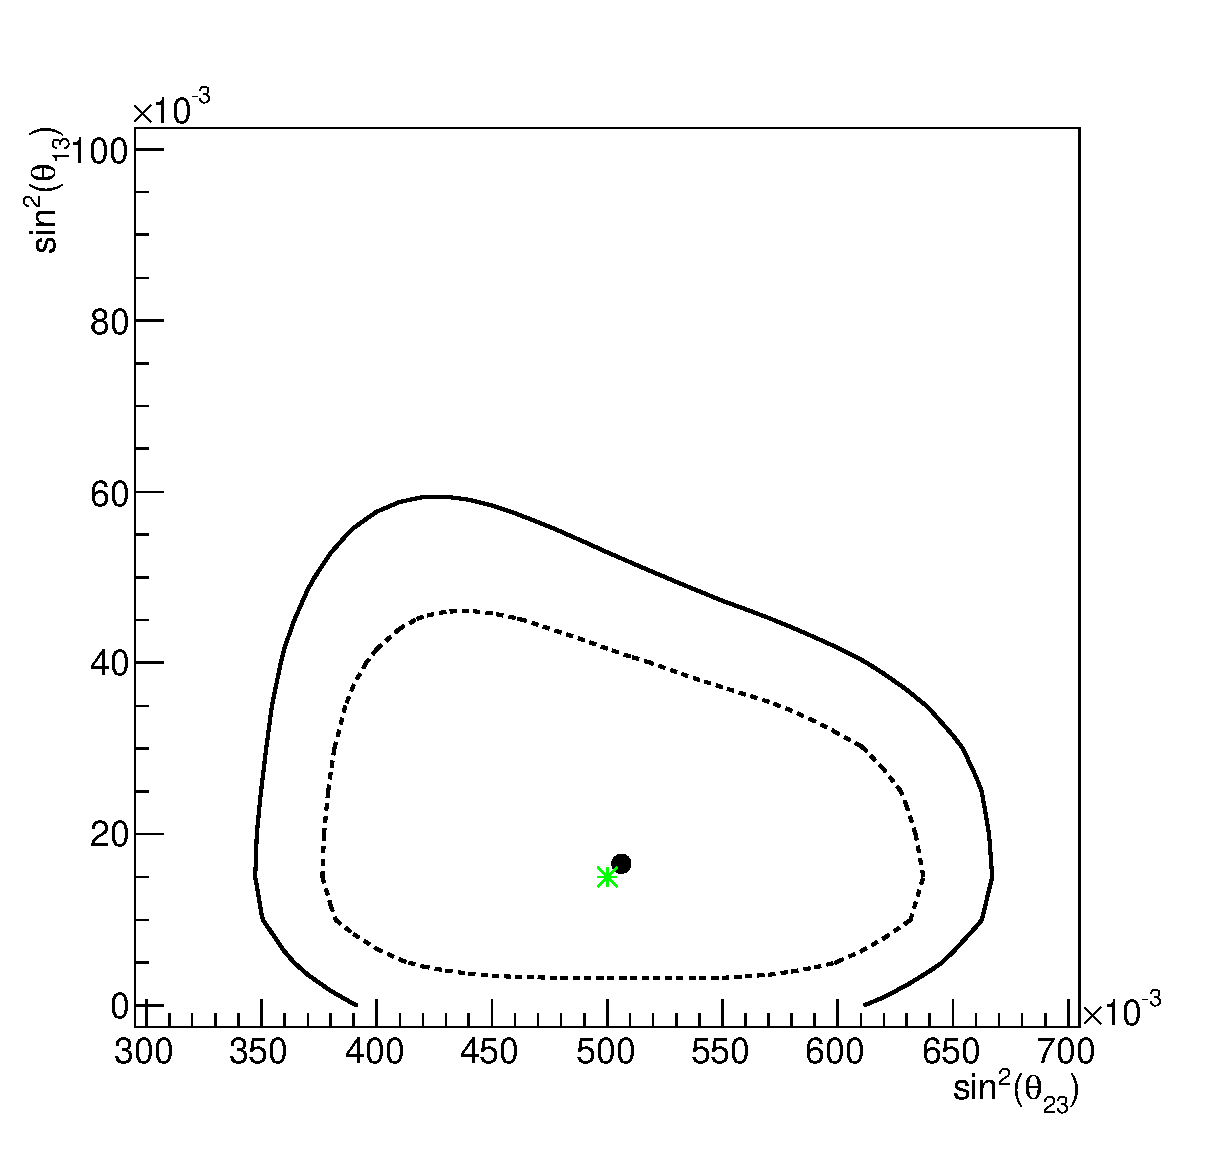
\includegraphics[width=15pc]{./images/appendix/fake_dataset_fits/fake_dataset3_chisq_theta13_theta23_global_min_new.eps}
\caption {
  68\% and 90\% CL regions in ($sin^{2}\theta_{23}$, $sin^{2}\theta_{13}$) space for fake dataset \#2.
  At each point, $\chi^2$ was minimized with respect to 
  all oscillation parameters not shown (and not considered to be fixed)
  and all relevant nuisance parameters.
}
\label{fig:toymc2_confreg_sinsqtheta23_sinsqtheta13}
\end{minipage}

\end{figure*}

%
%
% ..............................................
% Fake dataset #3
%
%

\clearpage

%
% delta\chisq and contours
%

\begin{figure*}[htb]

\begin{minipage}[t]{0.22\linewidth}
\center
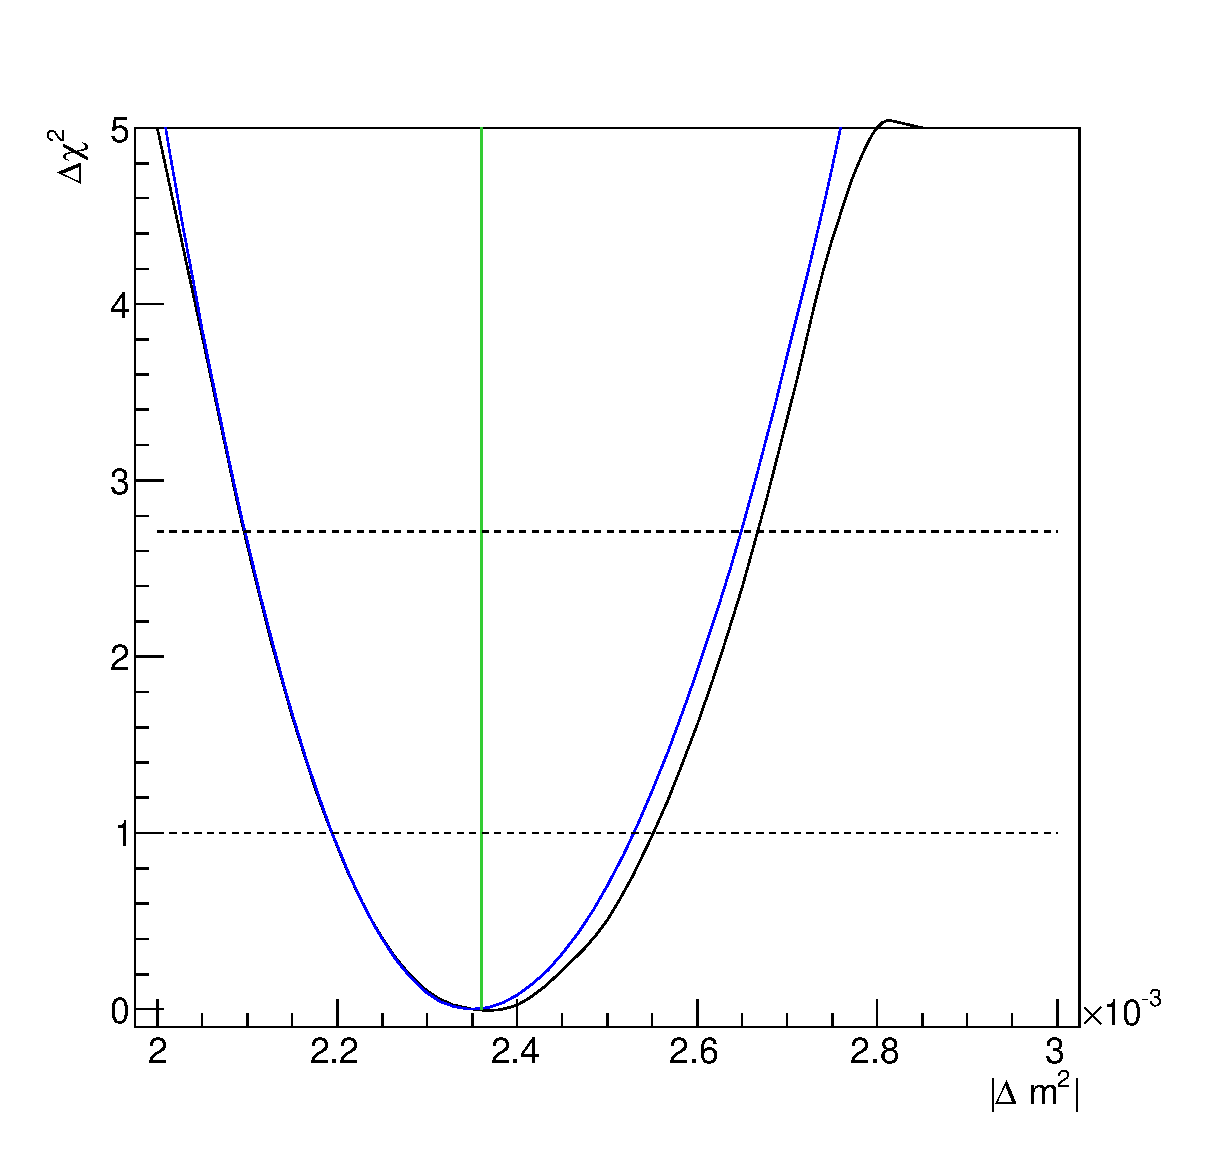
\includegraphics[width=9pc]{./images/appendix/fake_dataset_fits/fake_dataset5_chisq_dm23sq_global_min_new.eps}
\caption {
  $\Delta\chi^2$ as function of $|\Delta m^{2}|$ for fake dataset \#3.
  At each point, $\chi^2$ was minimized with respect to 
  $\sin^{2}\theta_{23}$, $\sin^{2}\theta_{13}$, $\delta_{CP}$
  and all relevant nuisance parameters for the joint analysis (black)
  and with respect to $\sin^{2}\theta_{23}$ and all relevant nuisance
  parameters for the disappearance analysis (blue).
}
\label{fig:toymc3_dchisq_Dmsq}
\end{minipage}
\hspace{0.02\linewidth}
\begin{minipage}[t]{0.22\linewidth}
\center
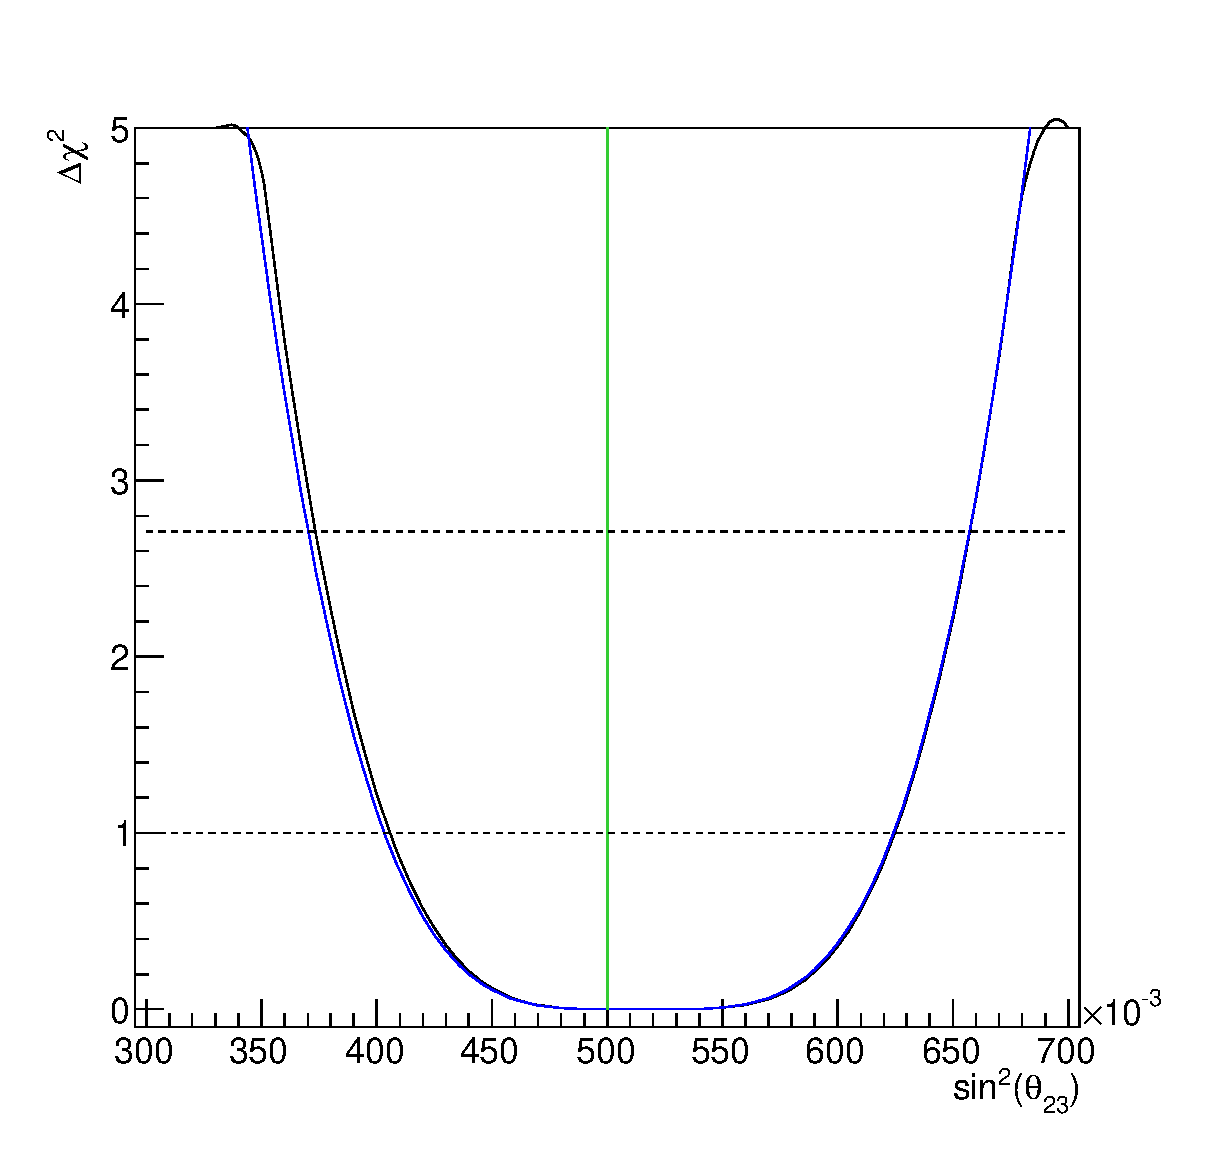
\includegraphics[width=9pc]{./images/appendix/fake_dataset_fits/fake_dataset5_chisq_theta23_global_min_new.eps}
\caption {
  $\Delta\chi^2$ as function of $sin^{2}\theta_{23}$ for fake dataset \#3.
  At each point, $\chi^2$ was minimized with respect to 
  $|\Delta m^{2}|$, $\sin^{2}\theta_{13}$, $\delta_{CP}$
  and all relevant nuisance parameters for the joint analysis (black)
  and with respect to $\sin^{2}\theta_{23}$ and all relevant nuisance
  parameters for the disappearance analysis (blue).
}
\label{fig:toymc3_dchisq_sinsqtheta23}
\end{minipage}
\hspace{0.02\linewidth}
\begin{minipage}[t]{0.22\linewidth}
\center
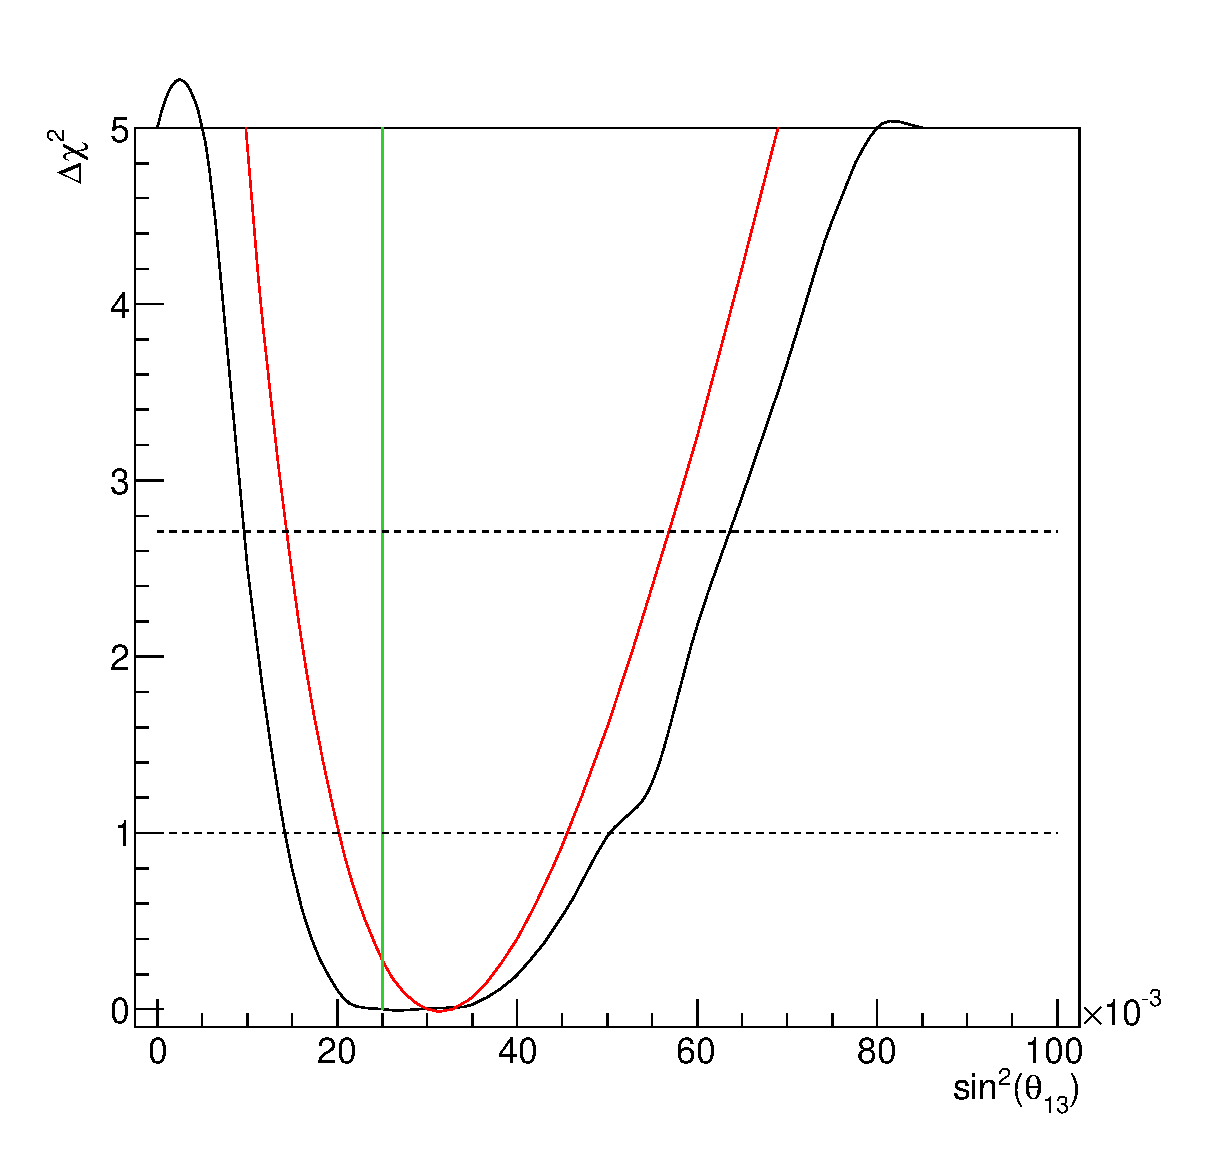
\includegraphics[width=9pc]{./images/appendix/fake_dataset_fits/fake_dataset5_chisq_theta13_global_min_new.eps}
\caption {
  $\Delta\chi^2$ as function of $sin^{2}\theta_{13}$ for fake dataset \#3.
  At each point, $\chi^2$ was minimized with respect to 
  $\sin^{2}\theta_{23}$, $\sin^{2}\theta_{13}$, $\delta_{CP}$
  and all relevant nuisance parameters for the joint analysis (black)
  and with respect to all relevant nuisance parameters 
  ($\delta_{CP}$ is fixed to 0) for the appearance analysis (red).
}
\label{fig:toymc3_dchisq_sinsqtheta13}
\end{minipage}
\hspace{0.02\linewidth}
\begin{minipage}[t]{0.22\linewidth}
\center
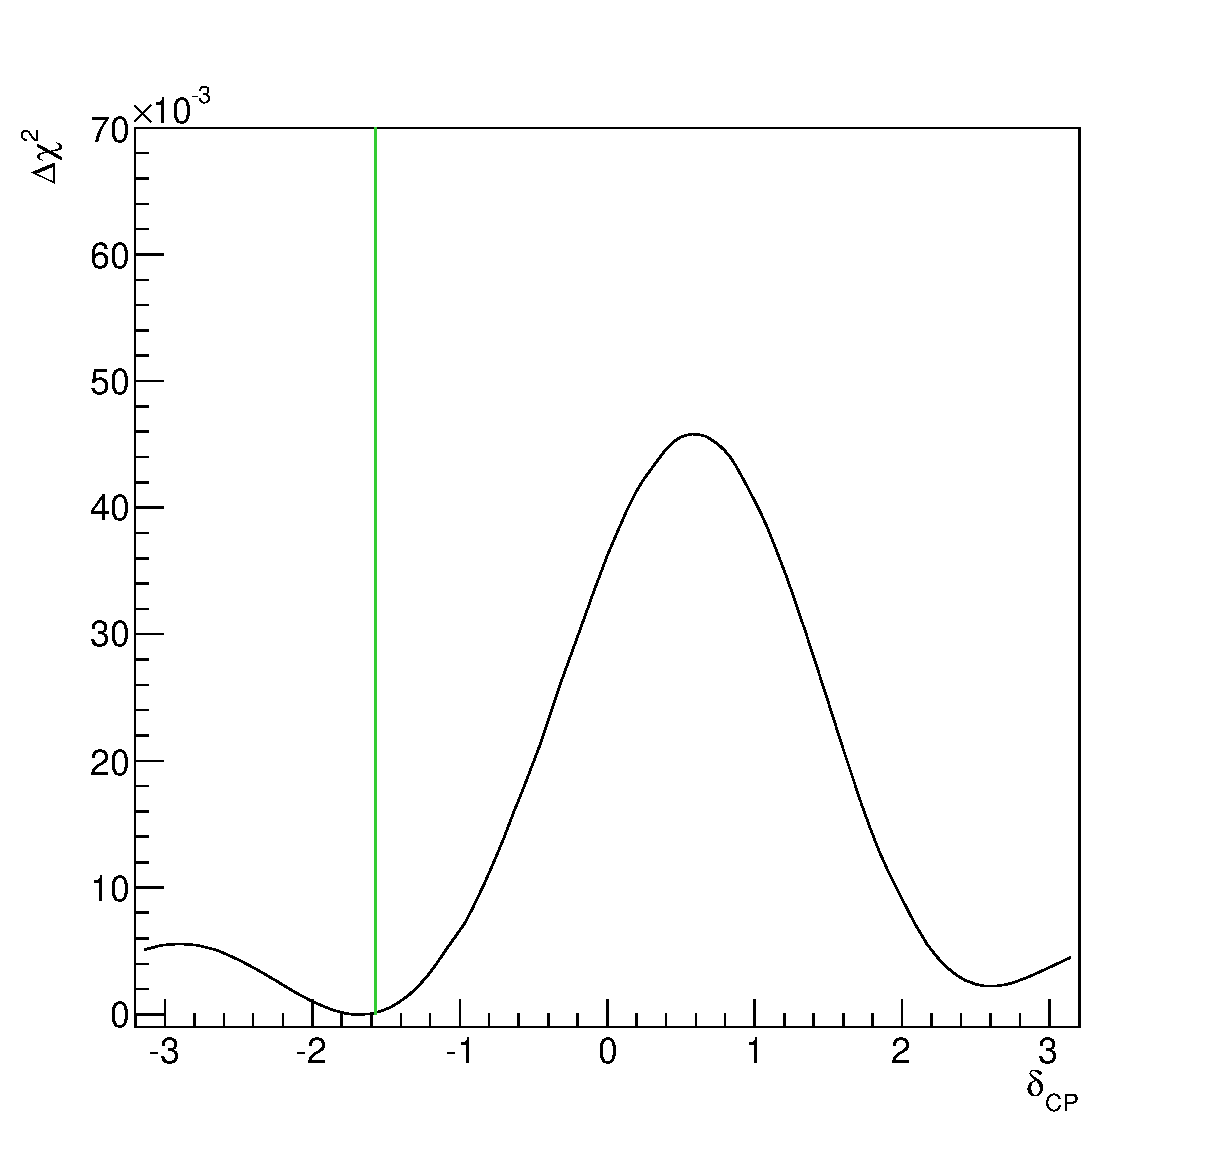
\includegraphics[width=9pc]{.//images/appendix/fake_dataset_fits/fake_dataset5_chisq_deltacp_global_min_new.eps}
\caption {
  $\Delta\chi^2$ as function of $\delta_{CP}$ for fake dataset \#3.
  At each point, $\chi^2$ was minimized with respect to 
  all oscillation parameters not shown (and not considered to be fixed)
  and all relevant nuisance parameters.
}
\label{fig:toymc3_dchisq_deltacp}
\end{minipage}
\vfill
\vspace*{0.7cm}
\begin{minipage}[t]{0.48\linewidth}
\center
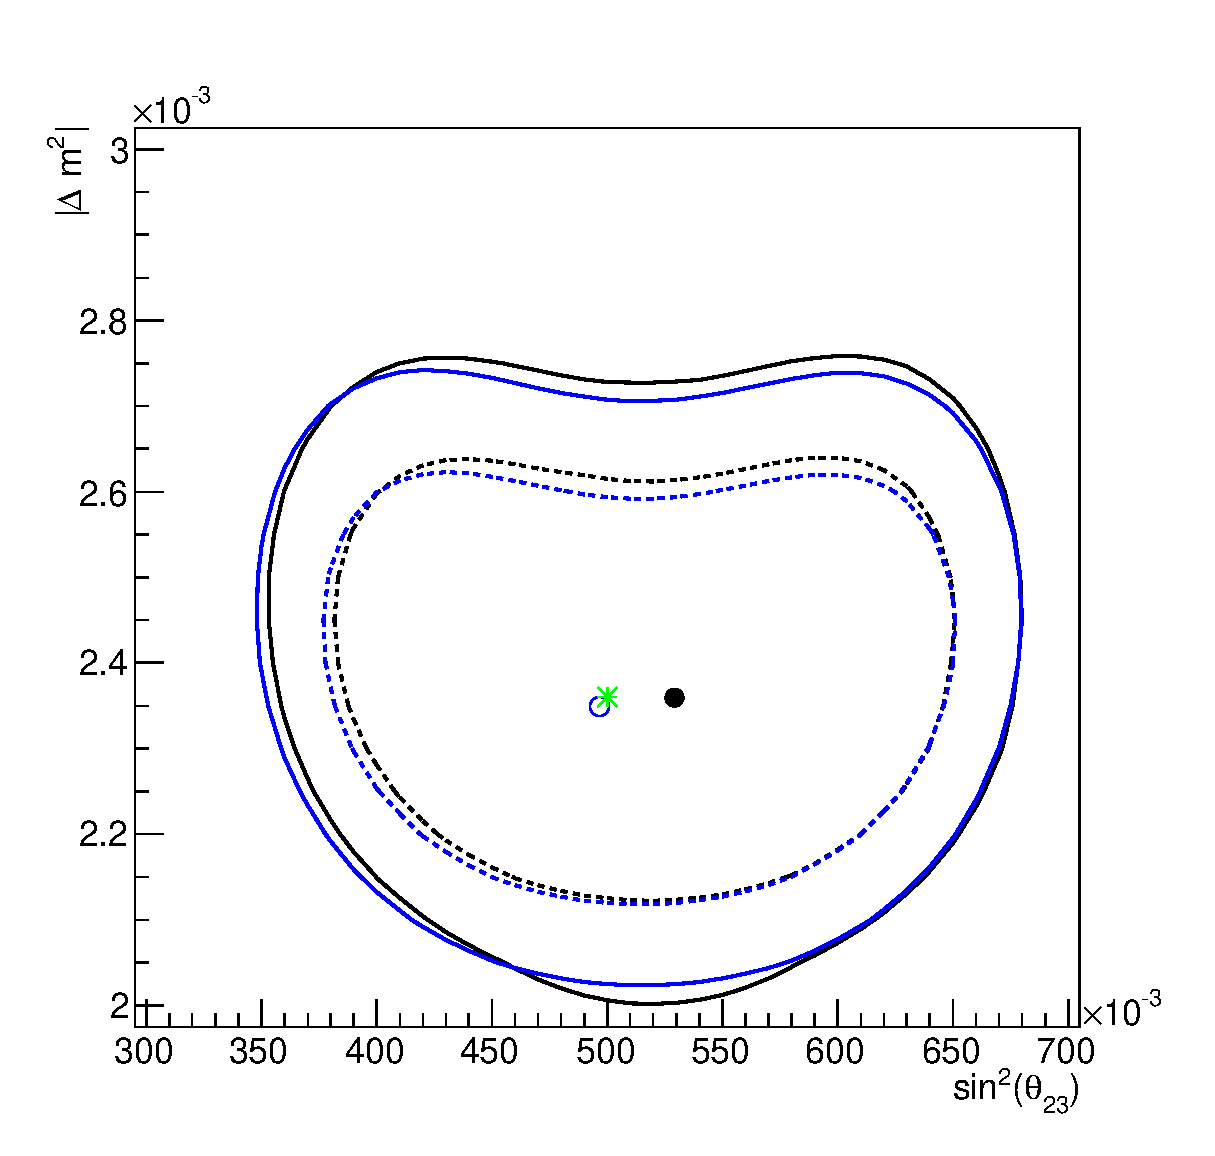
\includegraphics[width=15pc]{./images/appendix/fake_dataset_fits/fake_dataset5_chisq_theta23_dm23sq_global_min_new.eps}
\caption {
  68\% and 90\% CL regions in ($sin^{2}\theta_{23}$, $|\Delta m^{2}|$) space for fake dataset \#3.
  At each point, $\chi^2$ was minimized with respect to 
  $\sin^{2}\theta_{13}$, $\delta_{CP}$
  and all relevant nuisance parameters for the joint analysis (black)
  and with respect to all relevant nuisance parameters for the disappearance analysis (blue).
}
\label{fig:toymc3_confreg_sinsqtheta23_Dmsq}
\end{minipage}
\hspace{0.03\linewidth}
\begin{minipage}[t]{0.48\linewidth}
\center
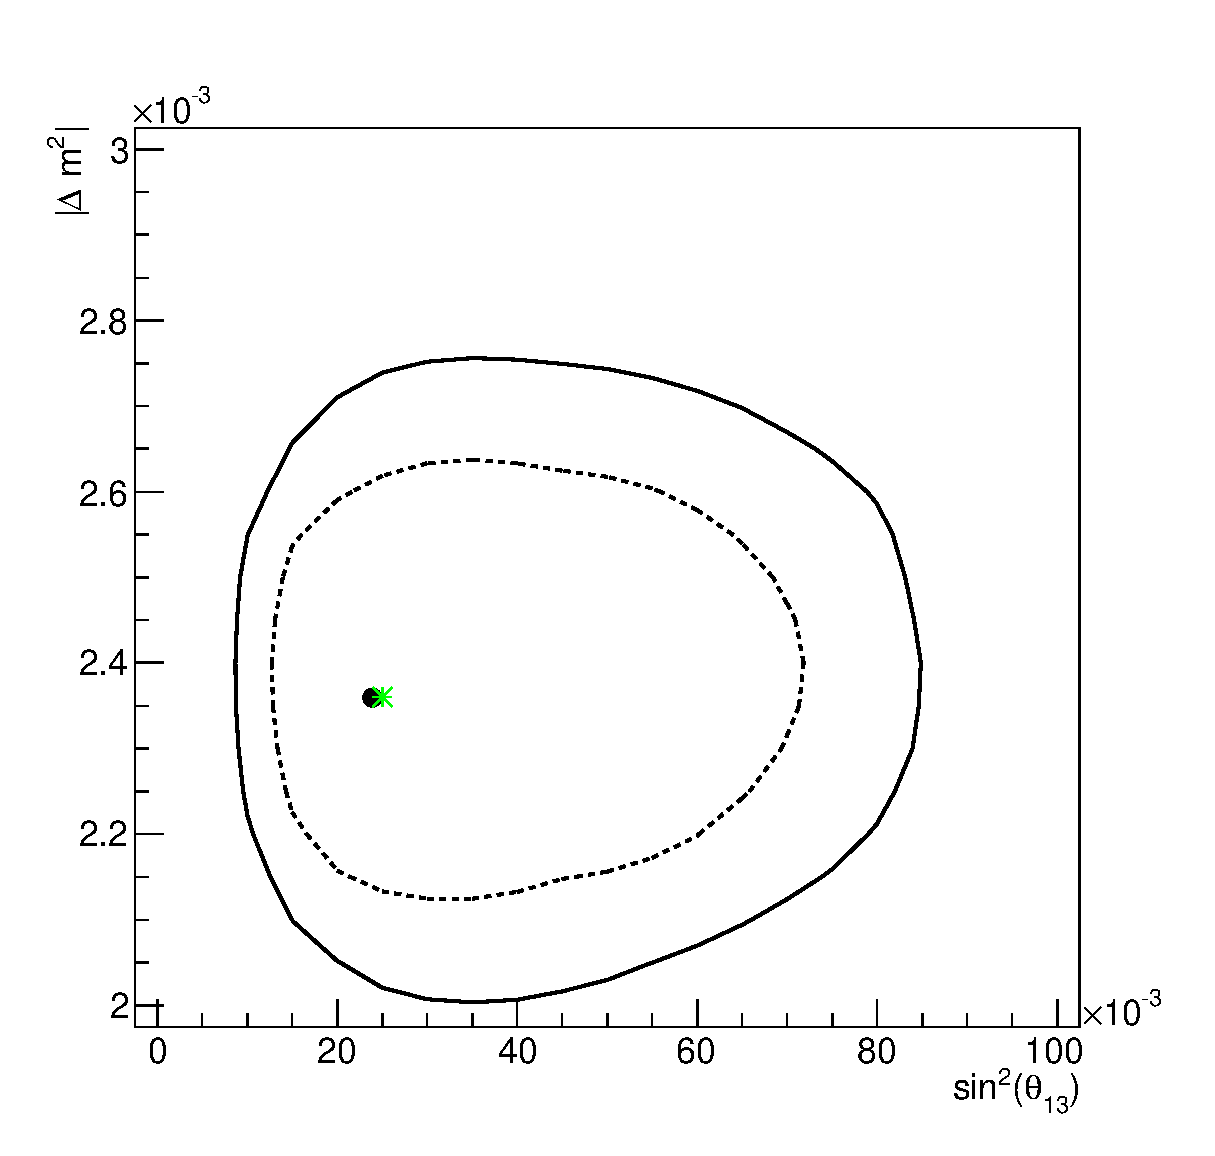
\includegraphics[width=15pc]{./images/appendix/fake_dataset_fits/fake_dataset5_chisq_theta13_dm23sq_global_min_new.eps}
\caption {
  68\% and 90\% CL regions in ($sin^{2}\theta_{13}$, $|\Delta m^{2}|$) space for fake dataset \#3.
  At each point, $\chi^2$ was minimized with respect to 
  all oscillation parameters not shown (and not considered to be fixed)
  and all relevant nuisance parameters.
}
\label{fig:toymc3_confreg_sinsqtheta13_Dmsq}
\end{minipage}
\vfill
\vspace*{0.7cm}
\begin{minipage}[t]{0.48\linewidth}
\center
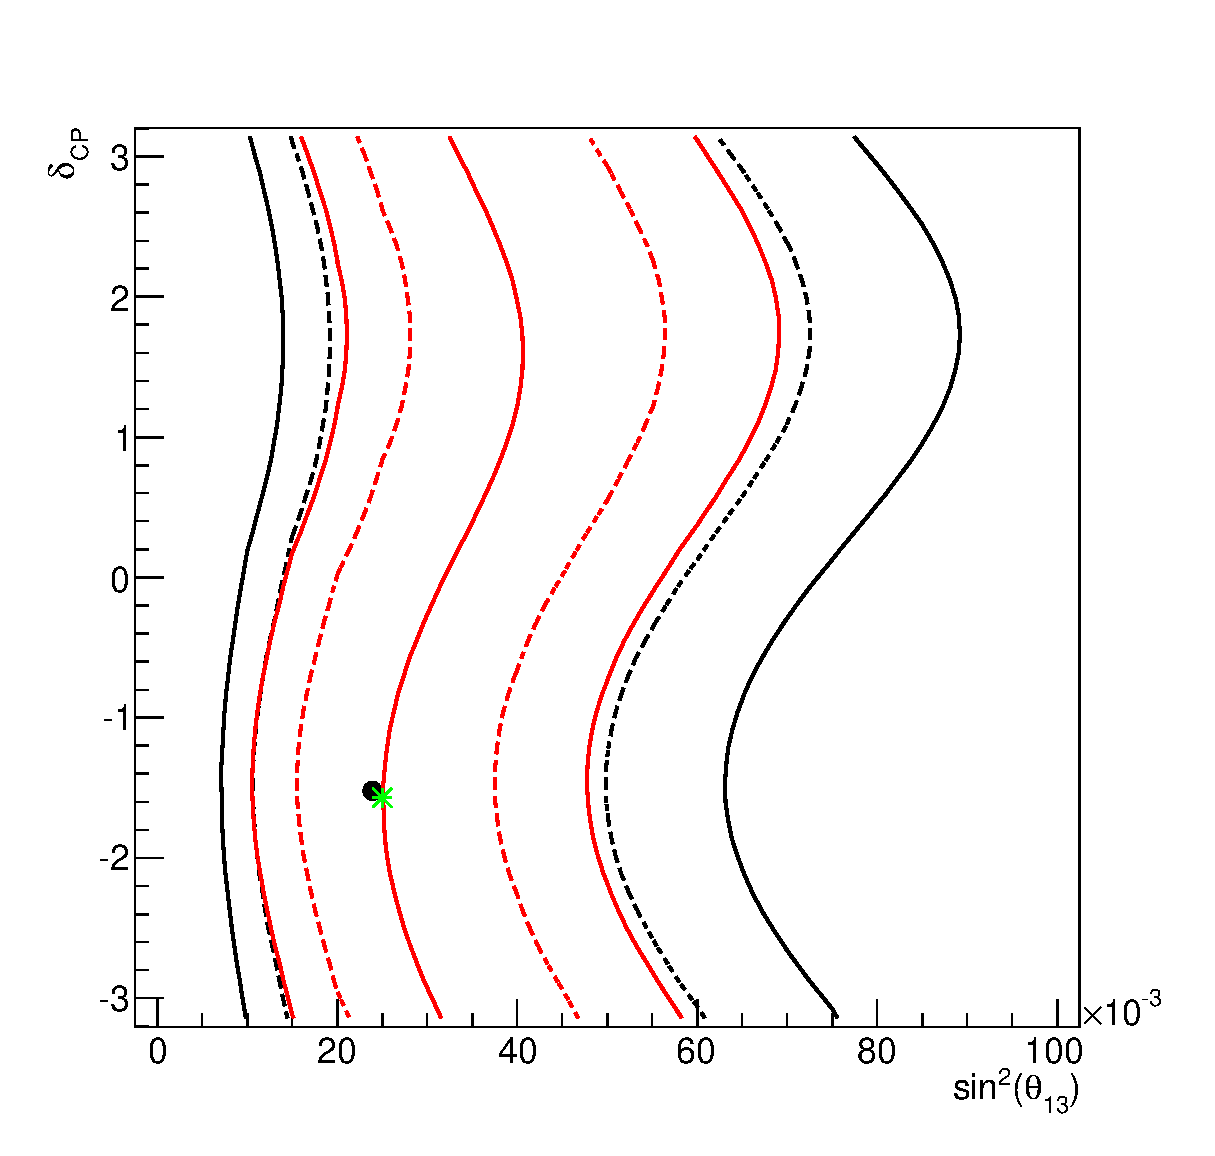
\includegraphics[width=15pc]{./images/appendix/fake_dataset_fits/fake_dataset5_chisq_theta13_deltacp_global_min_new.eps}
\caption {
  68\% and 90\% CL regions in ($sin^{2}\theta_{13}$, $\delta_{CP}$) space for fake dataset \#3.
  At each point, $\chi^2$ was minimized with respect to 
  $|\Delta m^{2}|$, $\sin^{2}\theta_{23}$
  and all relevant nuisance parameters for the joint analysis (black)
  and with respect to all relevant nuisance parameters for the appearance analysis (red).
  Notice that different methods are used to
  construct confidence regions for the joint analysis (global minimum) and for the 
  stand-alone appearance analysis (raster scan).
}
\label{fig:toymc3_confreg_sinsqtheta13_deltacp}
\end{minipage}
\hspace{0.03\linewidth}
\begin{minipage}[t]{0.48\linewidth}
\center
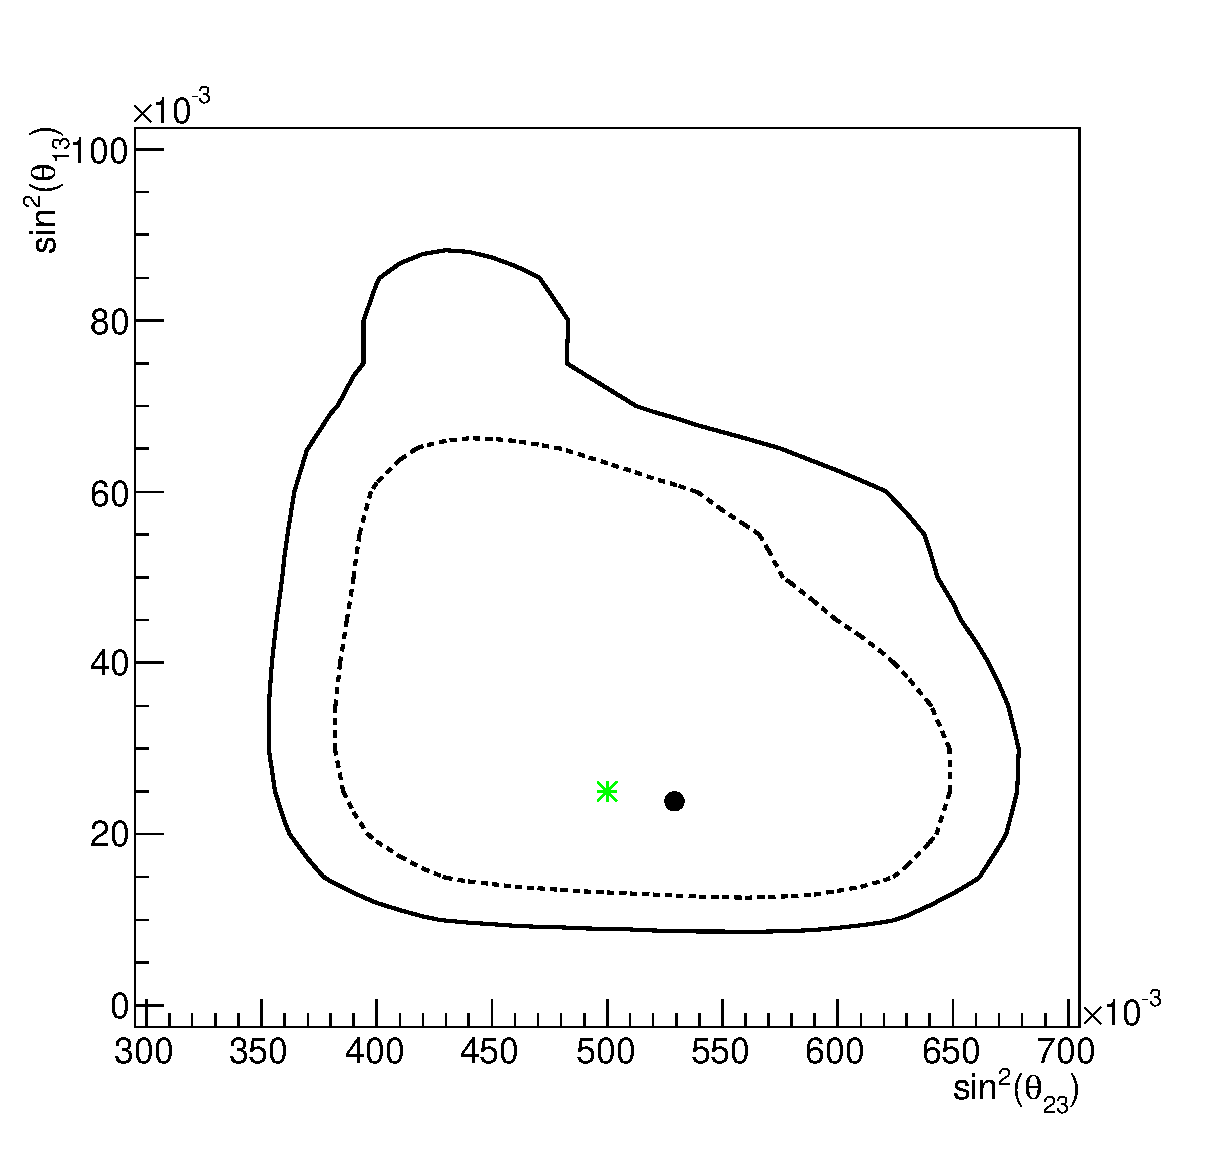
\includegraphics[width=15pc]{./images/appendix/fake_dataset_fits/fake_dataset5_chisq_theta13_theta23_global_min_new.eps}
\caption {
  68\% and 90\% CL regions in ($sin^{2}\theta_{23}$, $sin^{2}\theta_{13}$) space for fake dataset \#3.
  At each point, $\chi^2$ was minimized with respect to 
  all oscillation parameters not shown (and not considered to be fixed)
  and all relevant nuisance parameters.
}
\label{fig:toymc3_confreg_sinsqtheta23_sinsqtheta13}
\end{minipage}

\end{figure*}

%
%
% ..............................................
% Fake dataset #4
%
%

\clearpage

%
% delta\chisq and contours
%

\begin{figure*}[htb]

\begin{minipage}[t]{0.22\linewidth}
\center
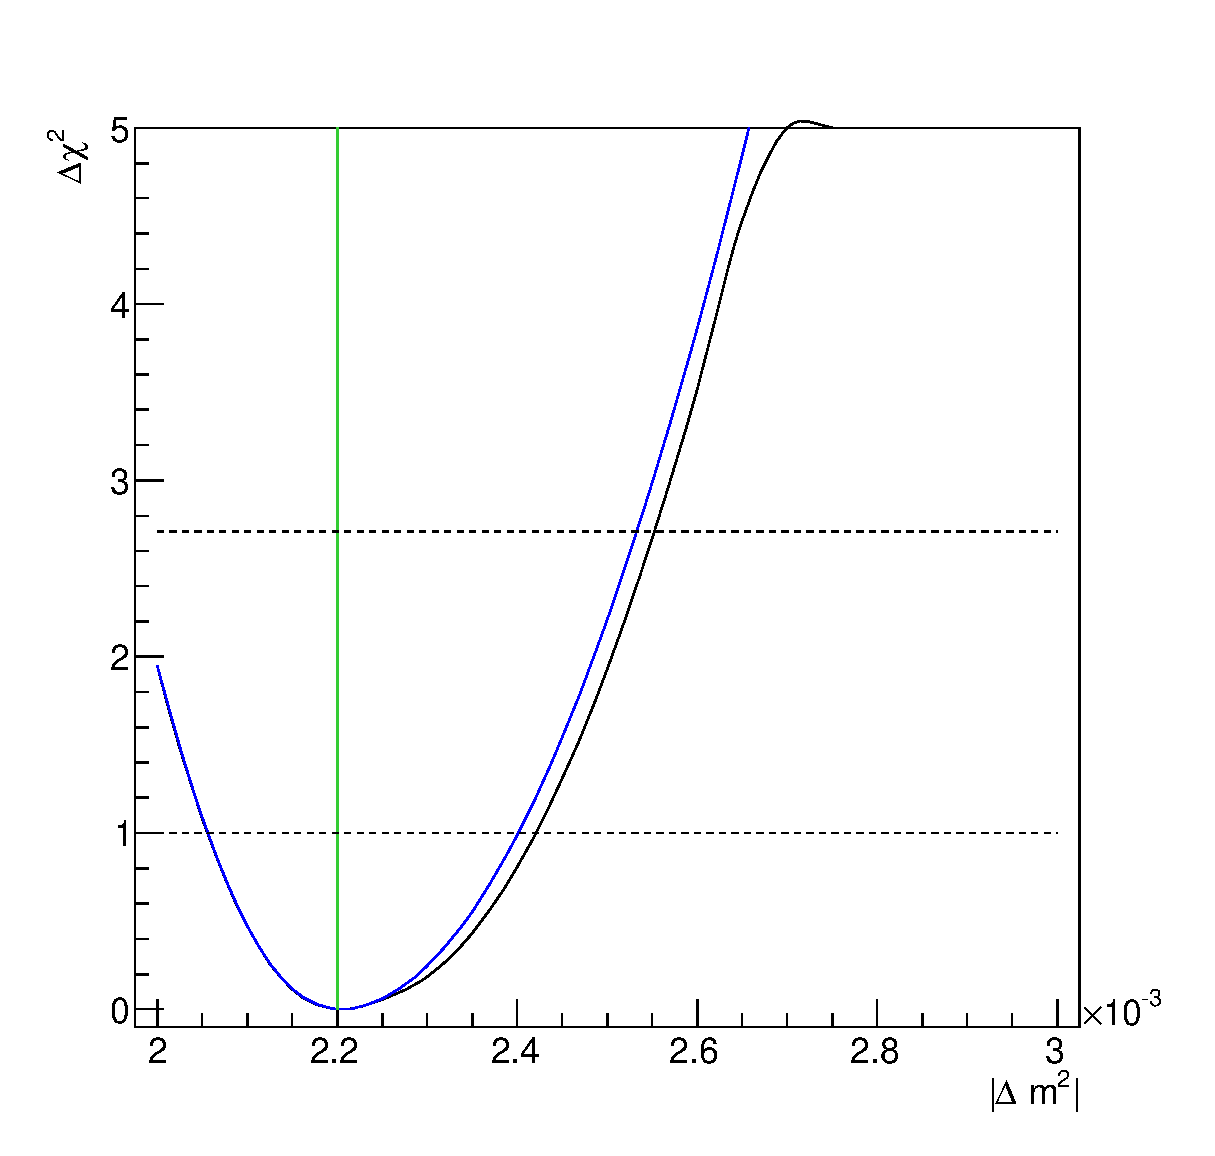
\includegraphics[width=9pc]{./images/appendix/fake_dataset_fits/fake_dataset7_chisq_dm23sq_global_min_new.eps}
\caption {
  $\Delta\chi^2$ as function of $|\Delta m^{2}|$ for fake dataset \#4.
  At each point, $\chi^2$ was minimized with respect to 
  $\sin^{2}\theta_{23}$, $\sin^{2}\theta_{13}$, $\delta_{CP}$
  and all relevant nuisance parameters for the joint analysis (black)
  and with respect to $\sin^{2}\theta_{23}$ and all relevant nuisance
  parameters for the disappearance analysis (blue).
}
\label{fig:toymc4_dchisq_Dmsq}
\end{minipage}
\hspace{0.02\linewidth}
\begin{minipage}[t]{0.22\linewidth}
\center
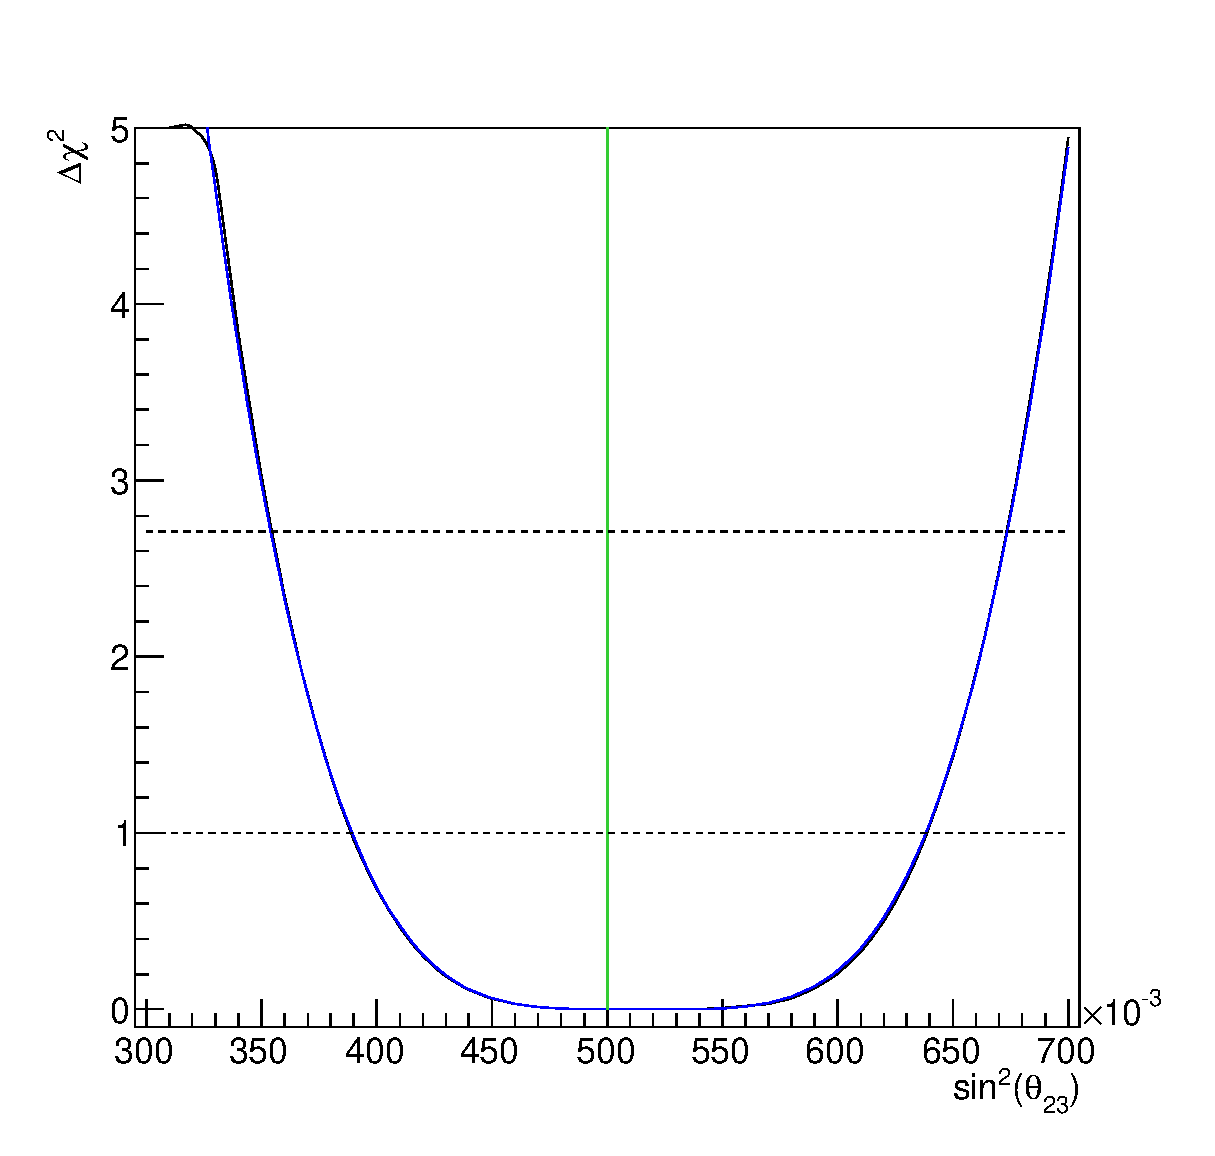
\includegraphics[width=9pc]{./images/appendix/fake_dataset_fits/fake_dataset7_chisq_theta23_global_min_new.eps}
\caption {
  $\Delta\chi^2$ as function of $sin^{2}\theta_{23}$ for fake dataset \#4.
  At each point, $\chi^2$ was minimized with respect to 
  $|\Delta m^{2}|$, $\sin^{2}\theta_{13}$, $\delta_{CP}$
  and all relevant nuisance parameters for the joint analysis (black)
  and with respect to $\sin^{2}\theta_{23}$ and all relevant nuisance
  parameters for the disappearance analysis (blue).
}
\label{fig:toymc4_dchisq_sinsqtheta23}
\end{minipage}
\hspace{0.02\linewidth}
\begin{minipage}[t]{0.22\linewidth}
\center
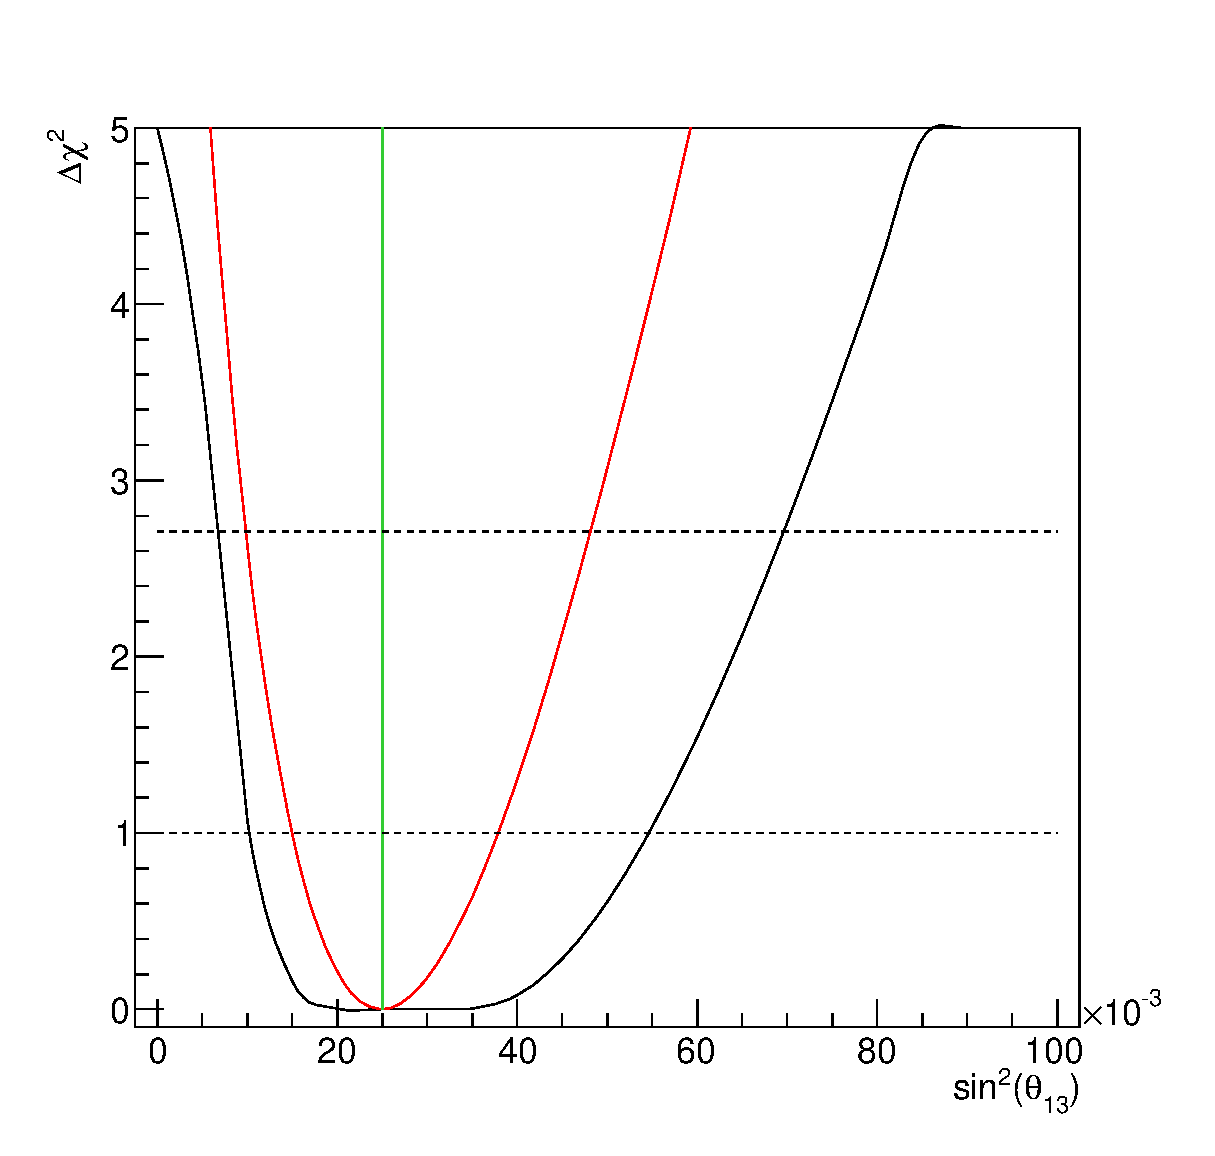
\includegraphics[width=9pc]{./images/appendix/fake_dataset_fits/fake_dataset7_chisq_theta13_global_min_new.eps}
\caption {
  $\Delta\chi^2$ as function of $sin^{2}\theta_{13}$ for fake dataset \#4.
  At each point, $\chi^2$ was minimized with respect to 
  $\sin^{2}\theta_{23}$, $\sin^{2}\theta_{13}$, $\delta_{CP}$
  and all relevant nuisance parameters for the joint analysis (black)
  and with respect to all relevant nuisance parameters 
  ($\delta_{CP}$ is fixed to 0) for the appearance analysis (red).
}
\label{fig:toymc4_dchisq_sinsqtheta13}
\end{minipage}
\hspace{0.02\linewidth}
\begin{minipage}[t]{0.22\linewidth}
\center
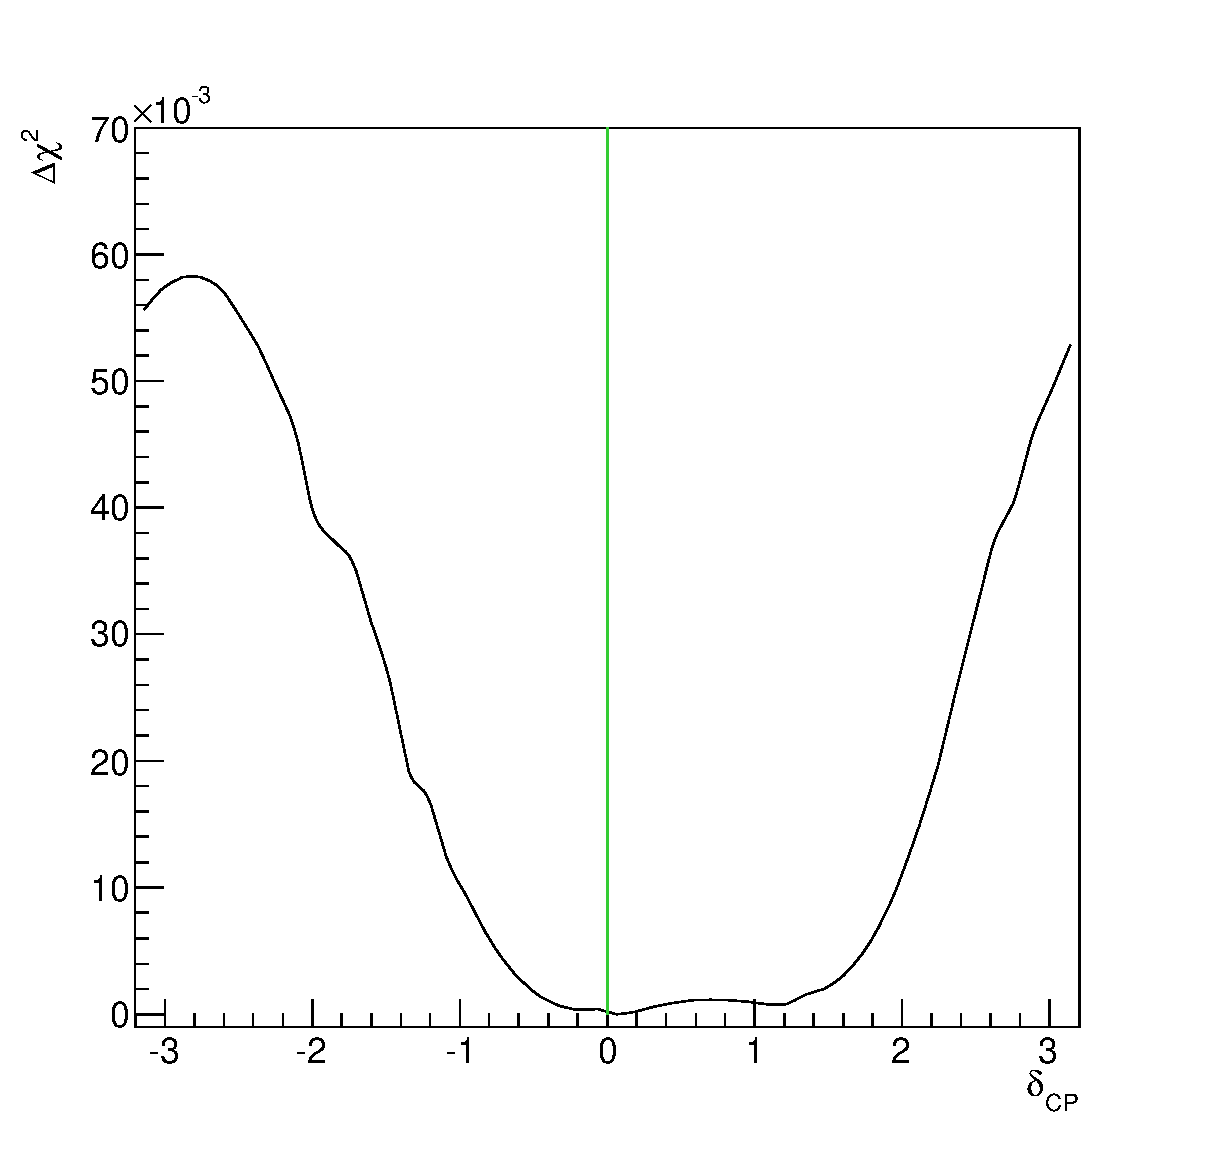
\includegraphics[width=9pc]{.//images/appendix/fake_dataset_fits/fake_dataset7_chisq_deltacp_global_min_new.eps}
\caption {
  $\Delta\chi^2$ as function of $\delta_{CP}$ for fake dataset \#4.
  At each point, $\chi^2$ was minimized with respect to 
  all oscillation parameters not shown (and not considered to be fixed)
  and all relevant nuisance parameters.
}
\label{fig:toymc4_dchisq_deltacp}
\end{minipage}

\vfill
\vspace*{0.7cm}

\begin{minipage}[t]{0.48\linewidth}
\center
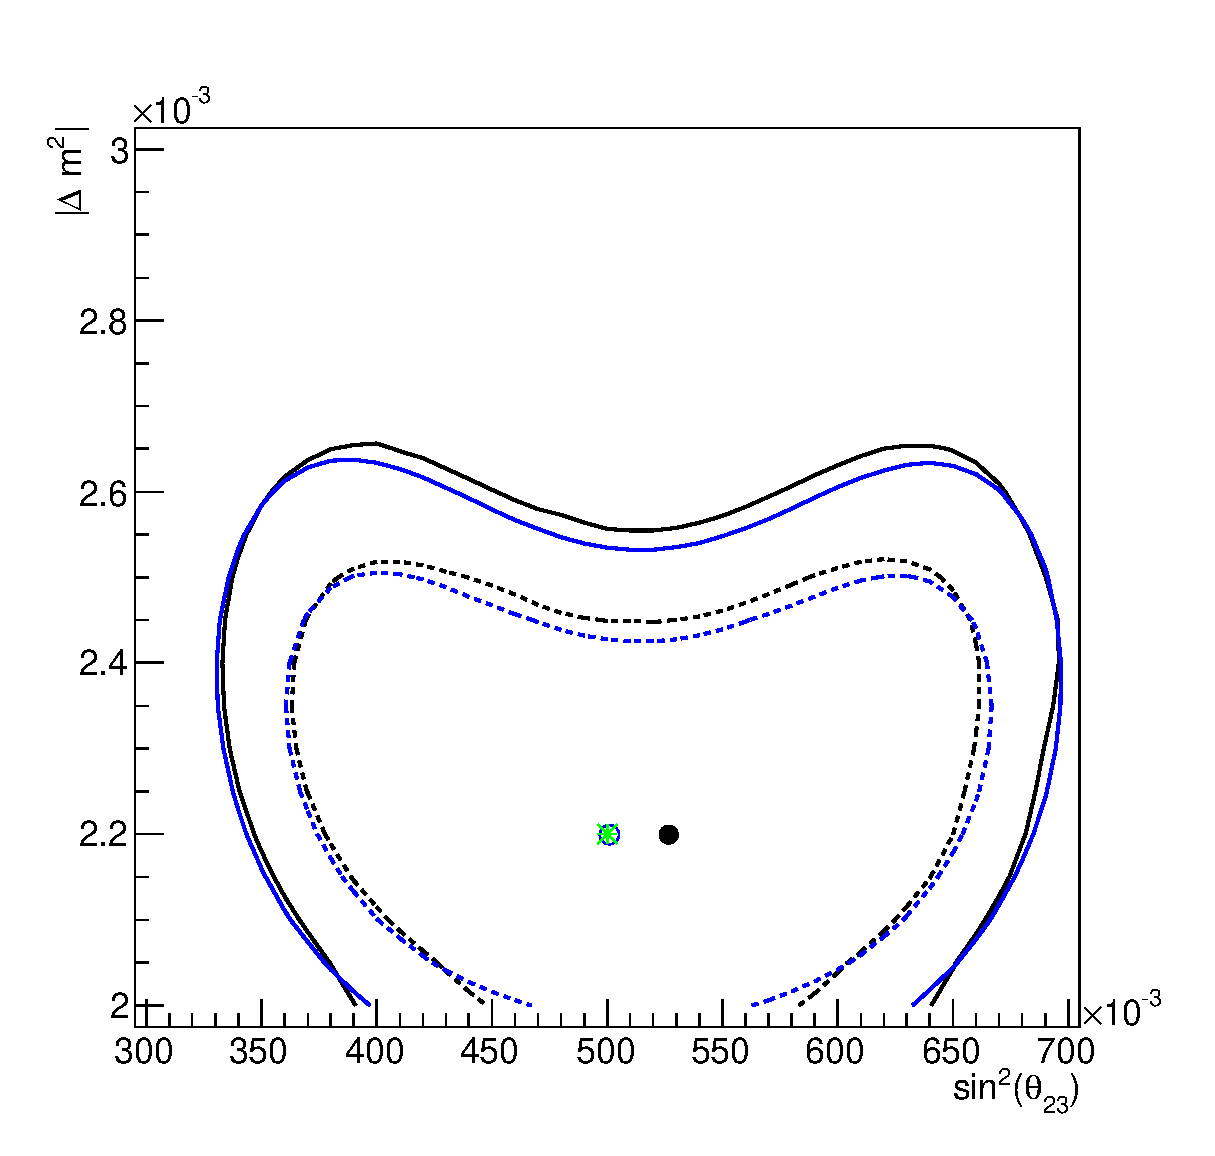
\includegraphics[width=15pc]{./images/appendix/fake_dataset_fits/fake_dataset7_chisq_theta23_dm23sq_global_min_new.eps}
\caption {
  68\% and 90\% CL regions in ($sin^{2}\theta_{23}$, $|\Delta m^{2}|$) space for fake dataset \#4.
  At each point, $\chi^2$ was minimized with respect to 
  $\sin^{2}\theta_{13}$, $\delta_{CP}$
  and all relevant nuisance parameters for the joint analysis (black)
  and with respect to all relevant nuisance parameters for the disappearance analysis (blue).
}
\label{fig:toymc4_confreg_sinsqtheta23_Dmsq}
\end{minipage}
\hspace{0.03\linewidth}
\begin{minipage}[t]{0.48\linewidth}
\center
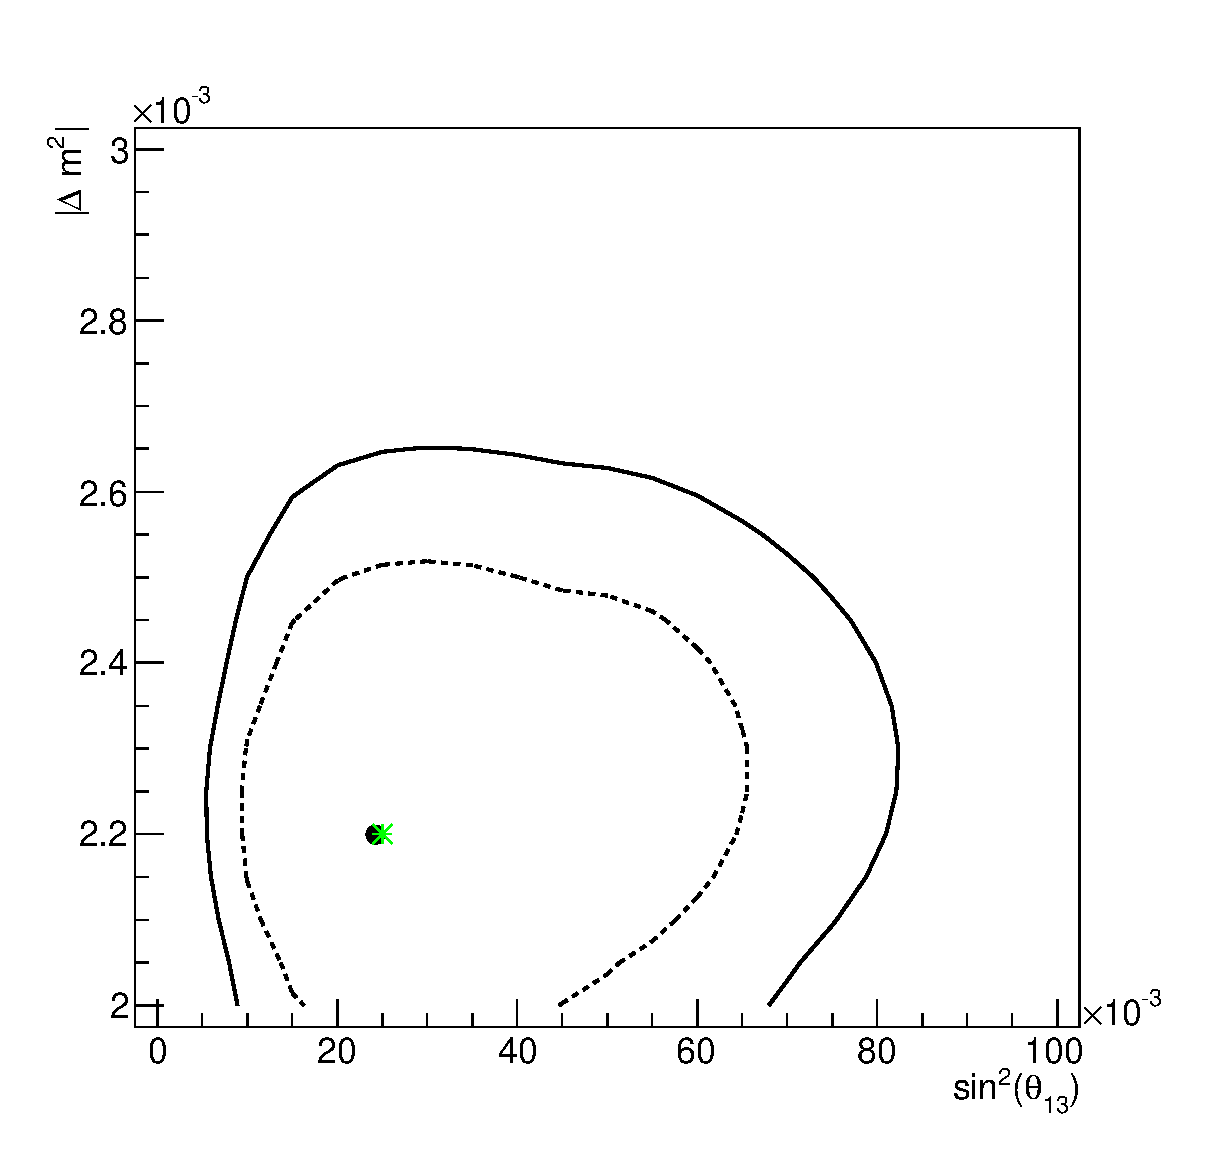
\includegraphics[width=15pc]{./images/appendix/fake_dataset_fits/fake_dataset7_chisq_theta13_dm23sq_global_min_new.eps}
\caption {
  68\% and 90\% CL regions in ($sin^{2}\theta_{13}$, $|\Delta m^{2}|$) space for fake dataset \#4.
  At each point, $\chi^2$ was minimized with respect to 
  all oscillation parameters not shown (and not considered to be fixed)
  and all relevant nuisance parameters.
}
\label{fig:toymc4_confreg_sinsqtheta13_Dmsq}
\end{minipage}

\vfill
\vspace*{0.7cm}

\begin{minipage}[t]{0.48\linewidth}
\center
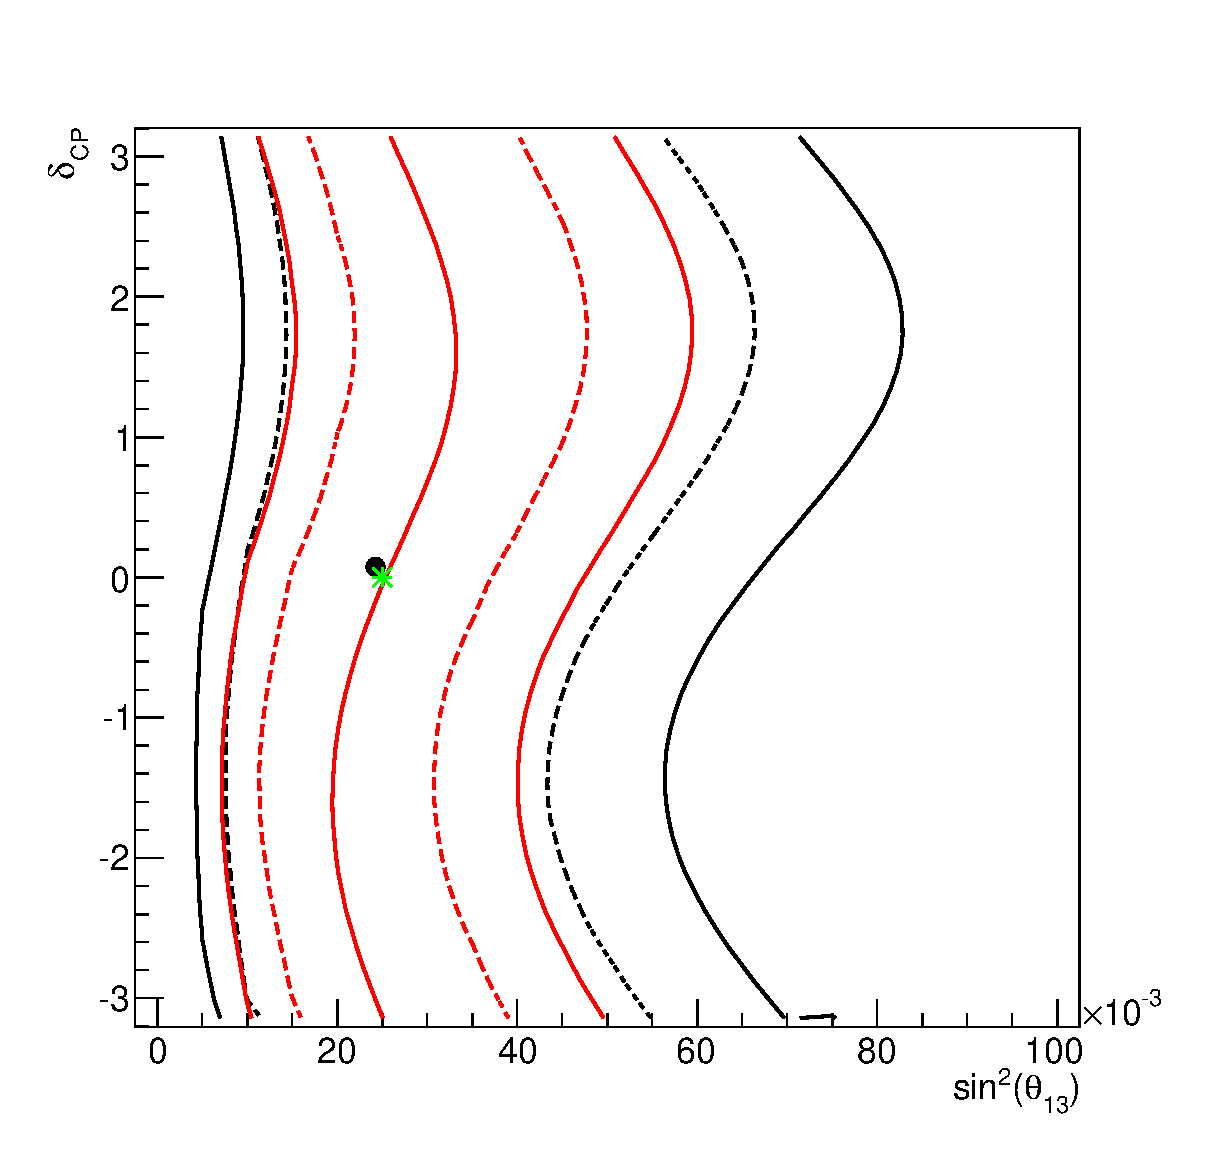
\includegraphics[width=15pc]{./images/appendix/fake_dataset_fits/fake_dataset7_chisq_theta13_deltacp_global_min_new.eps}
\caption {
  68\% and 90\% CL regions in ($sin^{2}\theta_{13}$, $\delta_{CP}$) space for fake dataset \#4.
  At each point, $\chi^2$ was minimized with respect to 
  $|\Delta m^{2}|$, $\sin^{2}\theta_{23}$
  and all relevant nuisance parameters for the joint analysis (black)
  and with respect to all relevant nuisance parameters for the appearance analysis (red).
  Notice that different methods are used to
  construct confidence regions for the joint analysis (global minimum) and for the 
  stand-alone appearance analysis (raster scan).
}
\label{fig:toymc4_confreg_sinsqtheta13_deltacp}
\end{minipage}
\hspace{0.03\linewidth}
\begin{minipage}[t]{0.48\linewidth}
\center
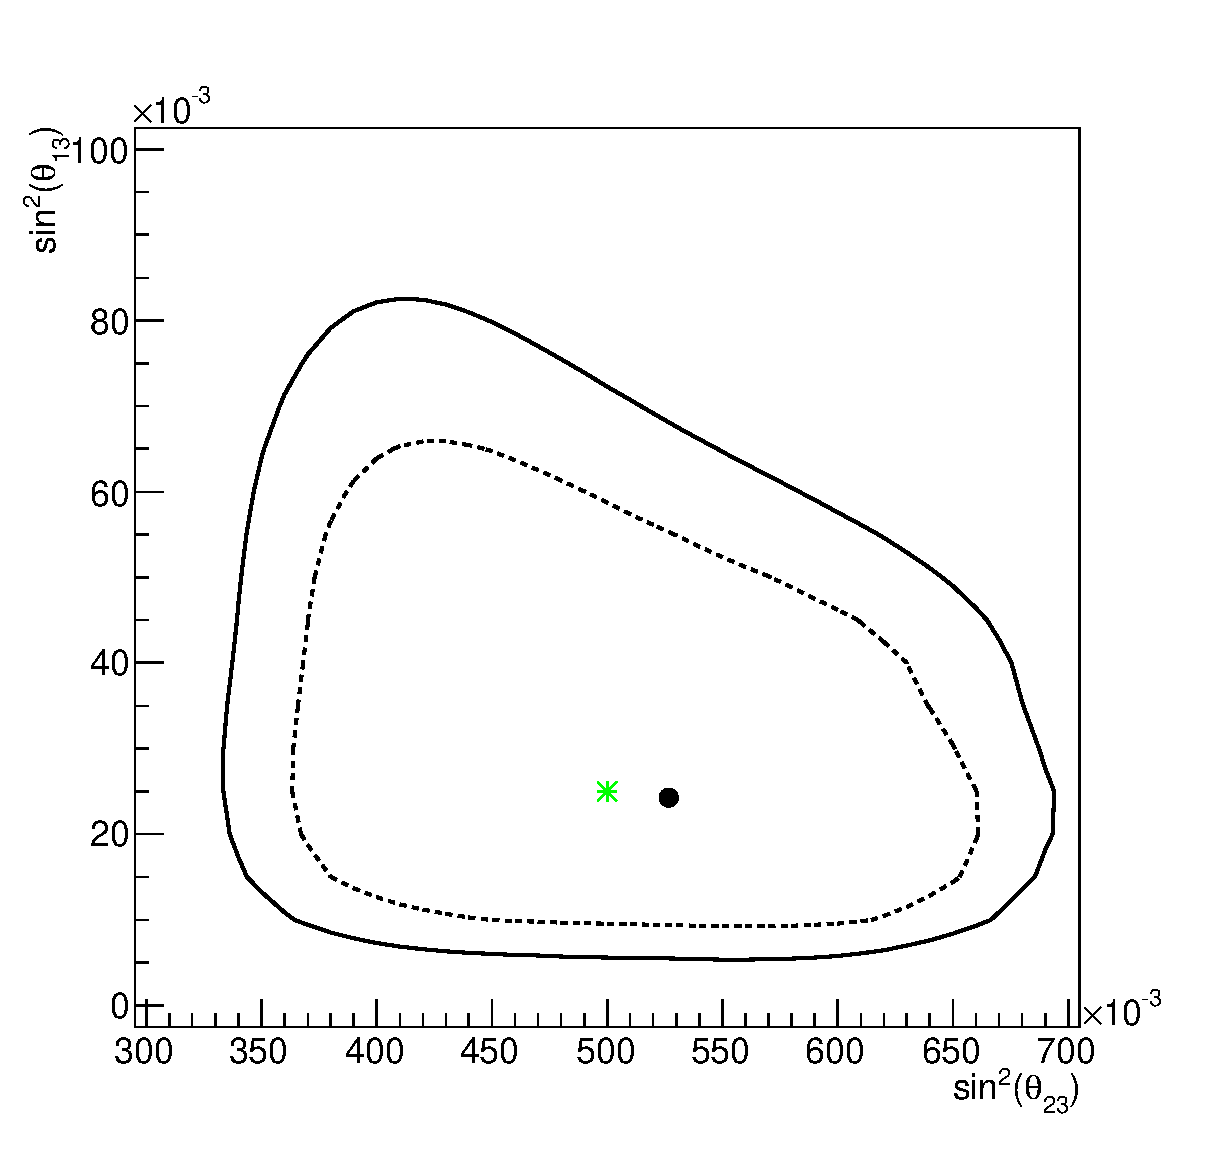
\includegraphics[width=15pc]{./images/appendix/fake_dataset_fits/fake_dataset7_chisq_theta13_theta23_global_min_new.eps}
\caption {
  68\% and 90\% CL regions in ($sin^{2}\theta_{23}$, $sin^{2}\theta_{13}$) space for fake dataset \#4.
  At each point, $\chi^2$ was minimized with respect to 
  all oscillation parameters not shown (and not considered to be fixed)
  and all relevant nuisance parameters.
}
\label{fig:toymc4_confreg_sinsqtheta23_sinsqtheta13}
\end{minipage}

\end{figure*}

% 
% 
% ..............................................
% Fake dataset #5 
% 
%

\clearpage

%
% delta\chisq and contours
%

\begin{figure*}[htb]

\begin{minipage}[t]{0.22\linewidth}
\center
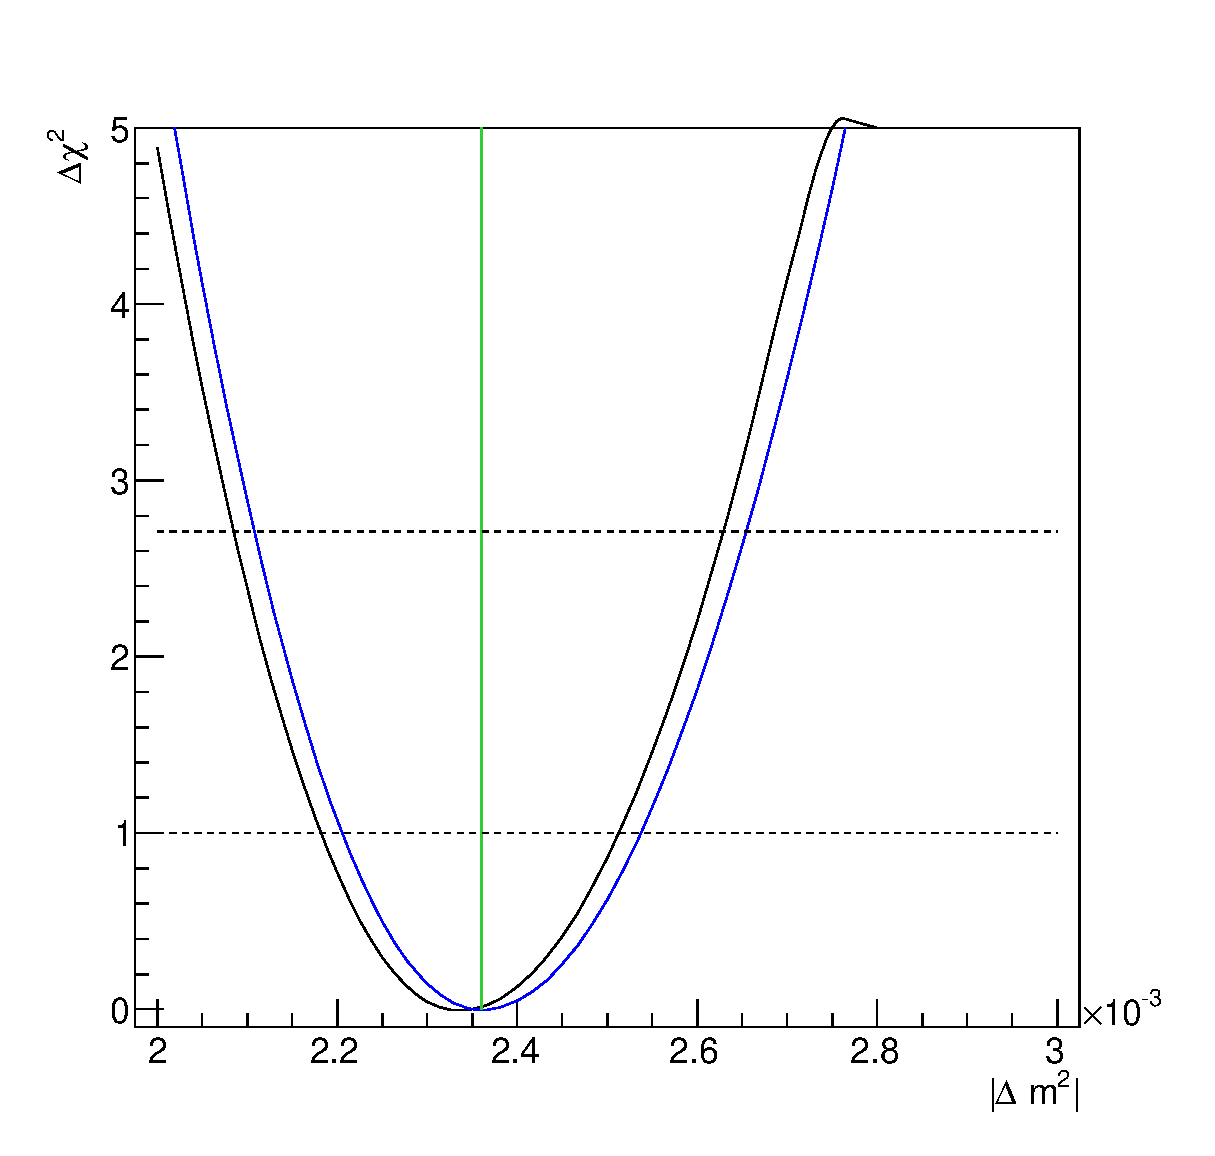
\includegraphics[width=9pc]{./images/appendix/fake_dataset_fits/fake_dataset9_chisq_dm23sq_global_min_new.eps}
\caption {
  $\Delta\chi^2$ as function of $|\Delta m^{2}|$ for fake dataset \#5.
  At each point, $\chi^2$ was minimized with respect to 
  $\sin^{2}\theta_{23}$, $\sin^{2}\theta_{13}$, $\delta_{CP}$
  and all relevant nuisance parameters for the joint analysis (black)
  and with respect to $\sin^{2}\theta_{23}$ and all relevant nuisance
  parameters for the disappearance analysis (blue).
}
\label{fig:toymc5_dchisq_Dmsq}
\end{minipage}
\hspace{0.02\linewidth}
\begin{minipage}[t]{0.22\linewidth}
\center
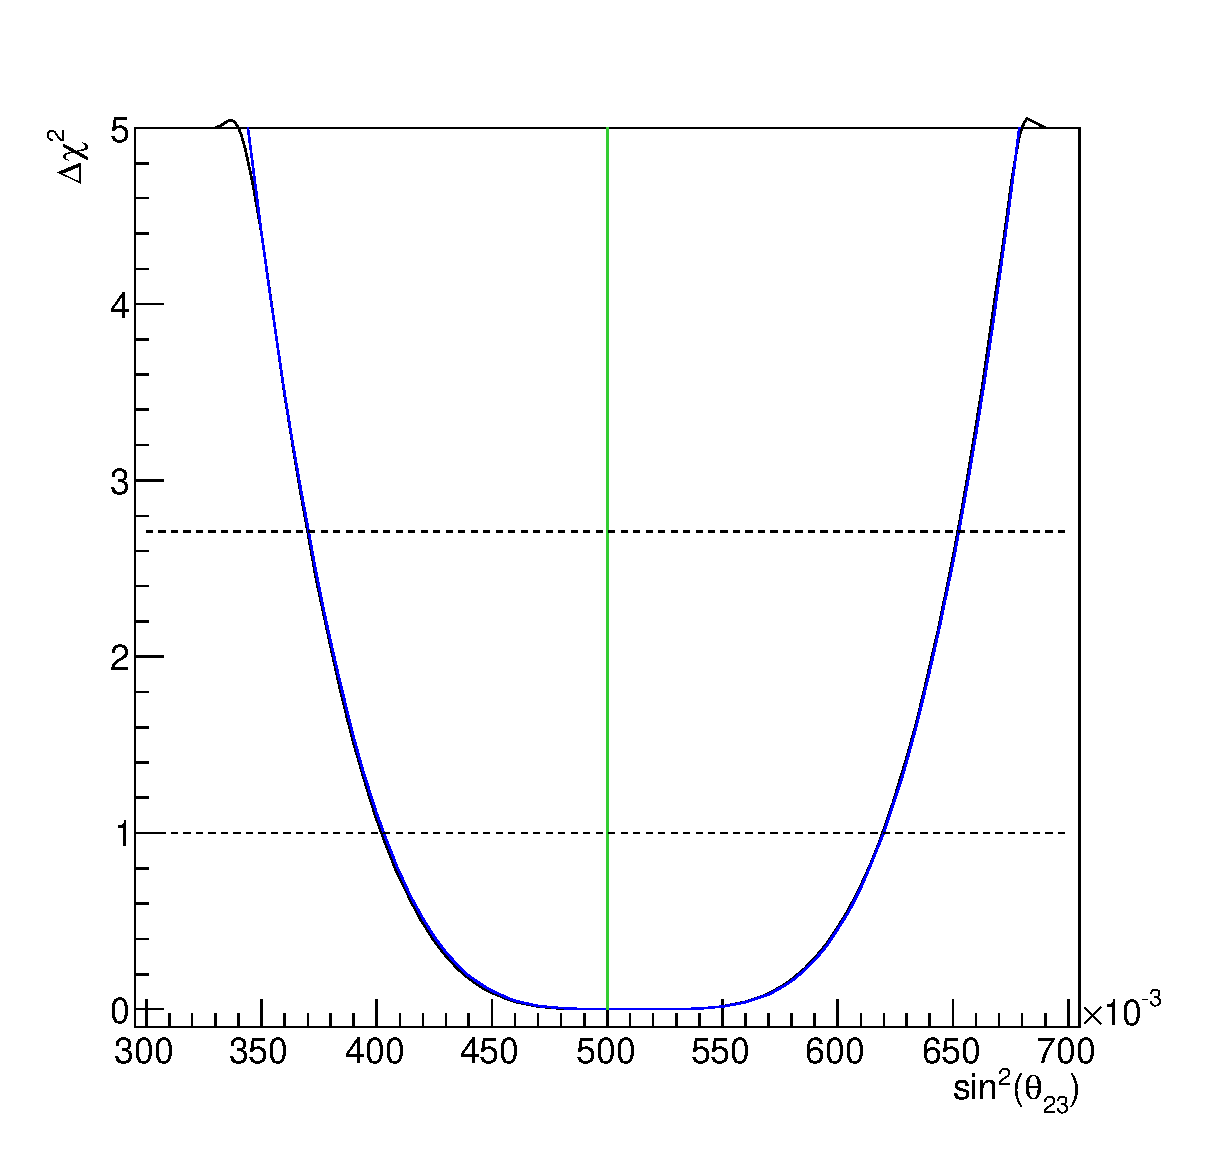
\includegraphics[width=9pc]{./images/appendix/fake_dataset_fits/fake_dataset9_chisq_theta23_global_min_new.eps}
\caption {
  $\Delta\chi^2$ as function of $sin^{2}\theta_{23}$ for fake dataset \#5.
  At each point, $\chi^2$ was minimized with respect to 
  $|\Delta m^{2}|$, $\sin^{2}\theta_{13}$, $\delta_{CP}$
  and all relevant nuisance parameters for the joint analysis (black)
  and with respect to $\sin^{2}\theta_{23}$ and all relevant nuisance
  parameters for the disappearance analysis (blue).
}
\label{fig:toymc5_dchisq_sinsqtheta23}
\end{minipage}
\hspace{0.02\linewidth}
\begin{minipage}[t]{0.22\linewidth}
\center
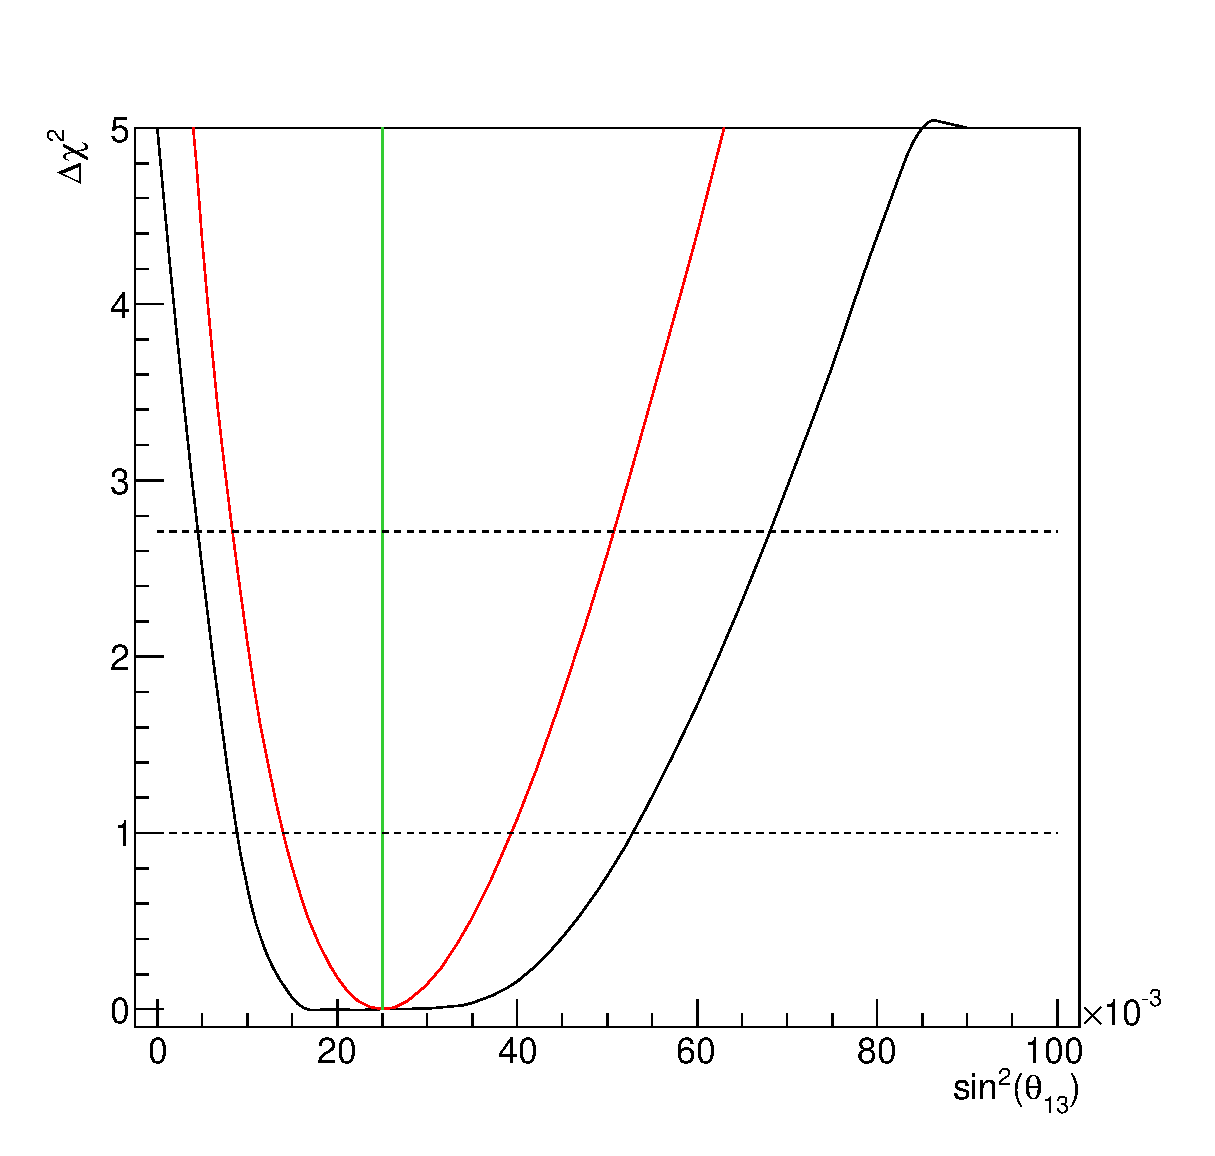
\includegraphics[width=9pc]{./images/appendix/fake_dataset_fits/fake_dataset9_chisq_theta13_global_min_new.eps}
\caption {
  $\Delta\chi^2$ as function of $sin^{2}\theta_{13}$ for fake dataset \#5.
  At each point, $\chi^2$ was minimized with respect to 
  $\sin^{2}\theta_{23}$, $\sin^{2}\theta_{13}$, $\delta_{CP}$
  and all relevant nuisance parameters for the joint analysis (black)
  and with respect to all relevant nuisance parameters 
  ($\delta_{CP}$ is fixed to 0) for the appearance analysis (red).
}
\label{fig:toymc5_dchisq_sinsqtheta13}
\end{minipage}
\hspace{0.02\linewidth}
\begin{minipage}[t]{0.22\linewidth}
\center
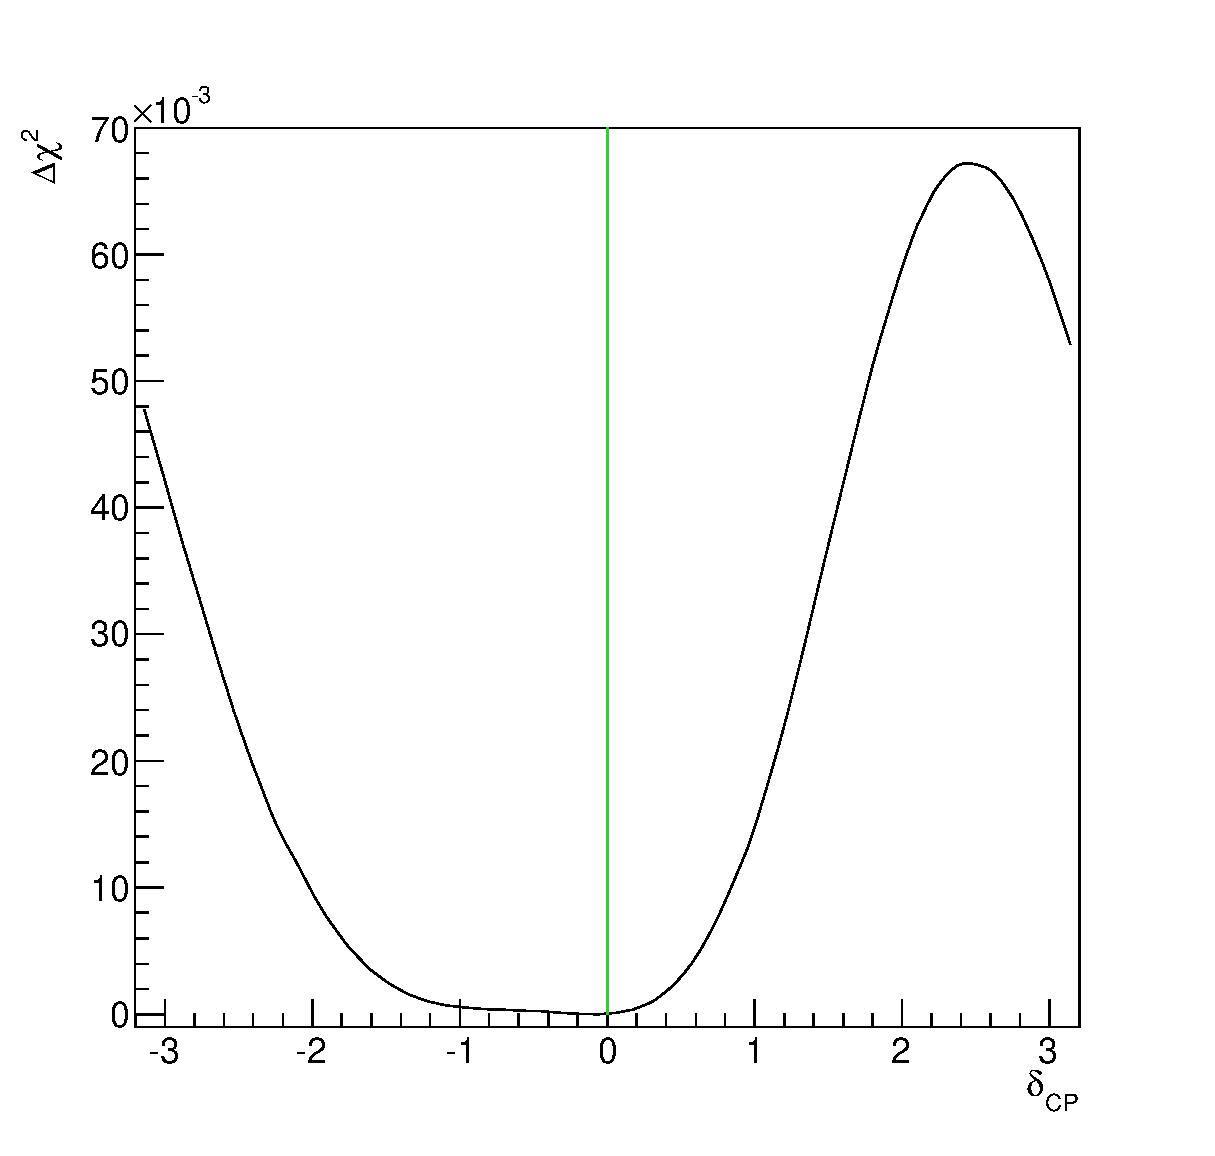
\includegraphics[width=9pc]{.//images/appendix/fake_dataset_fits/fake_dataset9_chisq_deltacp_global_min_new.eps}
\caption {
  $\Delta\chi^2$ as function of $\delta_{CP}$ for fake dataset \#5.
  At each point, $\chi^2$ was minimized with respect to 
  all oscillation parameters not shown (and not considered to be fixed)
  and all relevant nuisance parameters.
}
\label{fig:toymc5_dchisq_deltacp}
\end{minipage}
\vfill
\vspace*{0.7cm}
\begin{minipage}[t]{0.48\linewidth}
\center
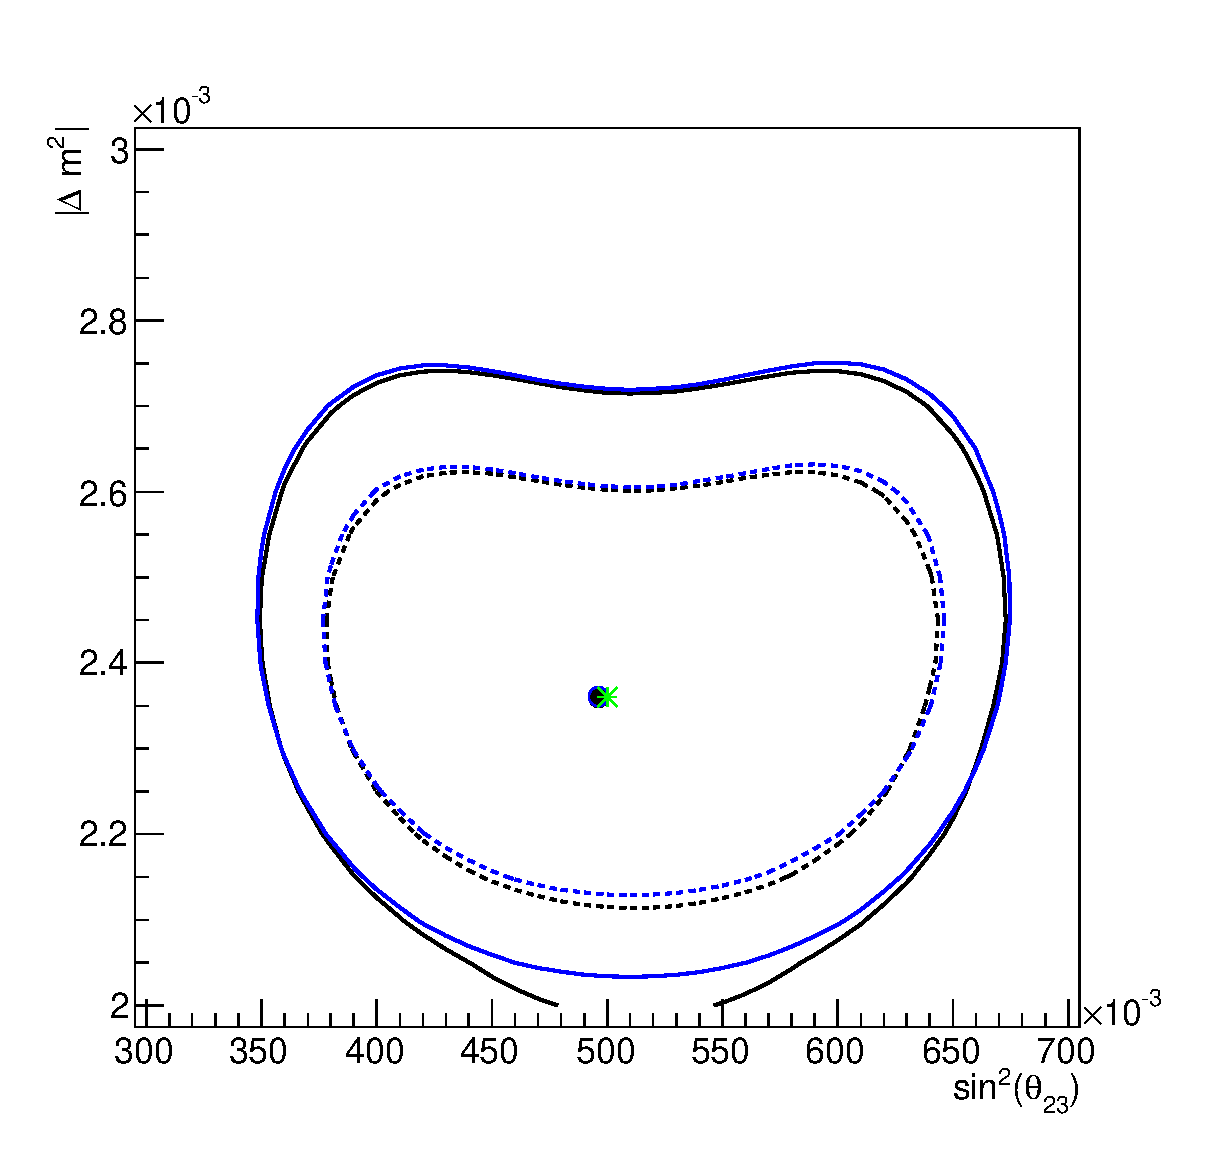
\includegraphics[width=15pc]{./images/appendix/fake_dataset_fits/fake_dataset9_chisq_theta23_dm23sq_global_min_new.eps}
\caption {
  68\% and 90\% CL regions in ($sin^{2}\theta_{23}$, $|\Delta m^{2}|$) space for fake dataset \#5.
  At each point, $\chi^2$ was minimized with respect to 
  $\sin^{2}\theta_{13}$, $\delta_{CP}$
  and all relevant nuisance parameters for the joint analysis (black)
  and with respect to all relevant nuisance parameters for the disappearance analysis (blue).
}
\label{fig:toymc5_confreg_sinsqtheta23_Dmsq}
\end{minipage}
\hspace{0.03\linewidth}
\begin{minipage}[t]{0.48\linewidth}
\center
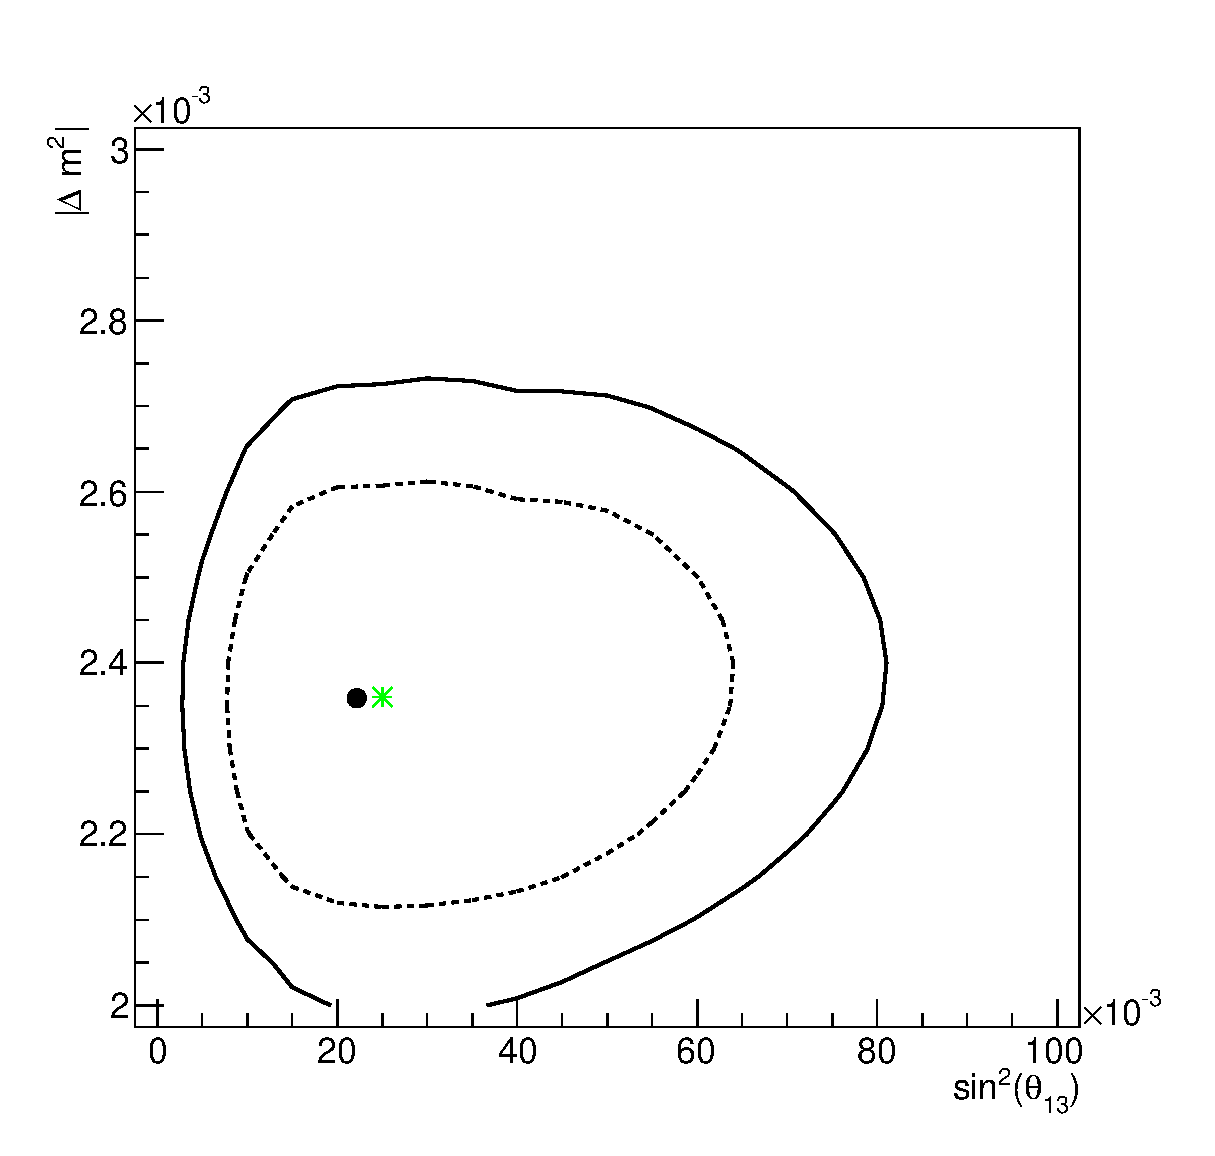
\includegraphics[width=15pc]{./images/appendix/fake_dataset_fits/fake_dataset9_chisq_theta13_dm23sq_global_min_new.eps}
\caption {
  68\% and 90\% CL regions in ($sin^{2}\theta_{13}$, $|\Delta m^{2}|$) space for fake dataset \#5.
  At each point, $\chi^2$ was minimized with respect to 
  all oscillation parameters not shown (and not considered to be fixed)
  and all relevant nuisance parameters.
}
\label{fig:toymc5_confreg_sinsqtheta13_Dmsq}
\end{minipage}

\vfill
\vspace*{0.7cm}

\begin{minipage}[t]{0.48\linewidth}
\center
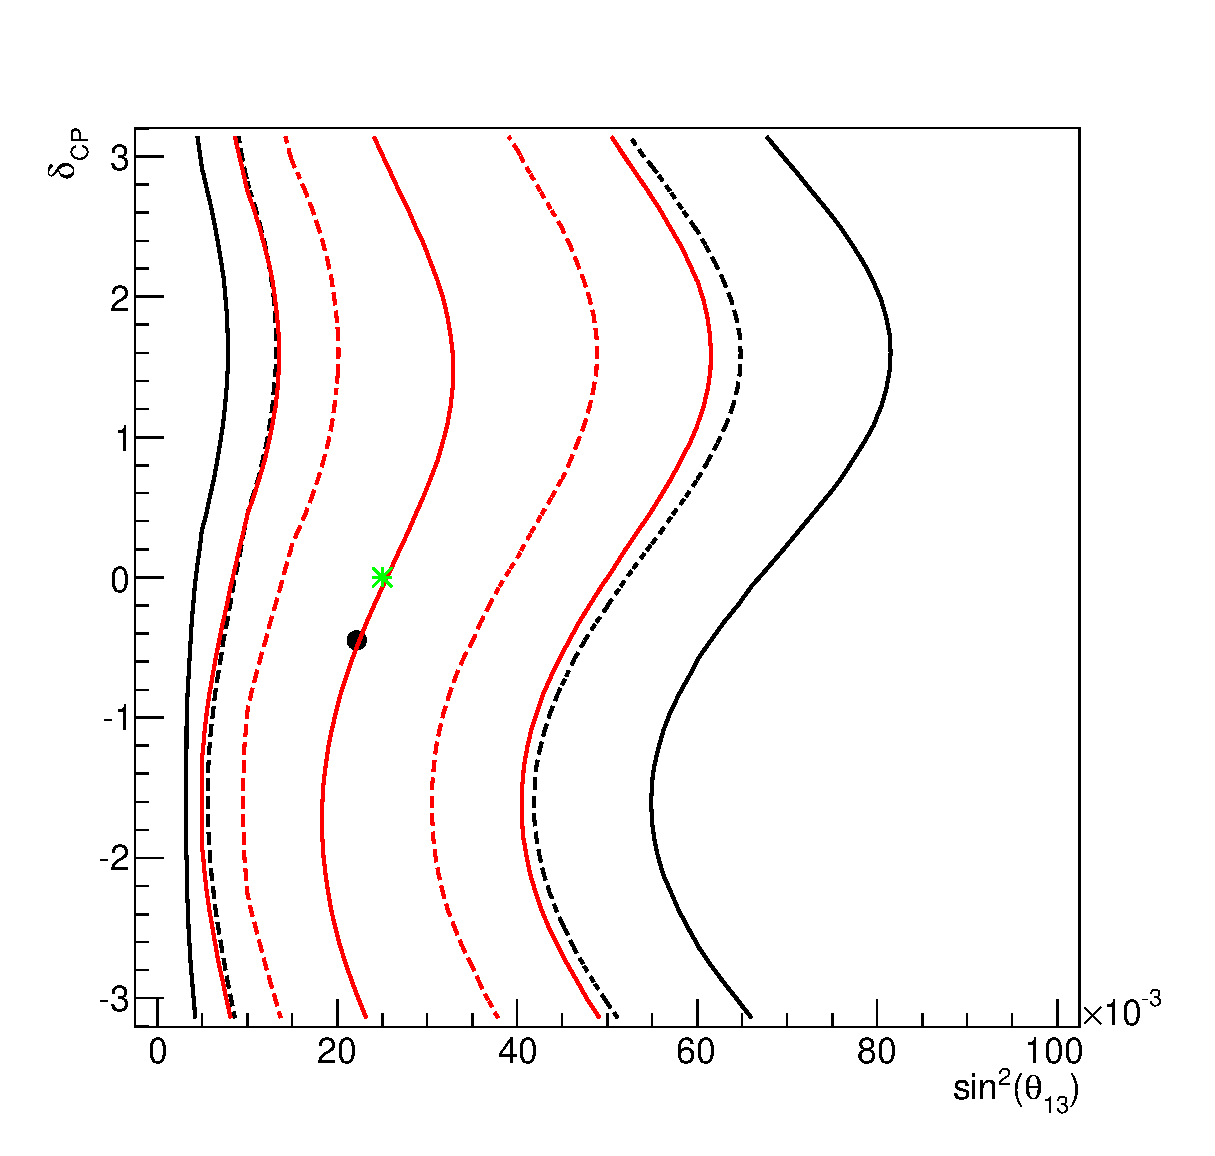
\includegraphics[width=15pc]{./images/appendix/fake_dataset_fits/fake_dataset9_chisq_theta13_deltacp_global_min_new.eps}
\caption {
  68\% and 90\% CL regions in ($sin^{2}\theta_{13}$, $\delta_{CP}$) space for fake dataset \#5.
  At each point, $\chi^2$ was minimized with respect to 
  $|\Delta m^{2}|$, $\sin^{2}\theta_{23}$
  and all relevant nuisance parameters for the joint analysis (black)
  and with respect to all relevant nuisance parameters for the appearance analysis (red).
  Notice that different methods are used to
  construct confidence regions for the joint analysis (global minimum) and for the 
  stand-alone appearance analysis (raster scan).
}
\label{fig:toymc5_confreg_sinsqtheta13_deltacp}
\end{minipage}
\hspace{0.03\linewidth}
\begin{minipage}[t]{0.48\linewidth}
\center
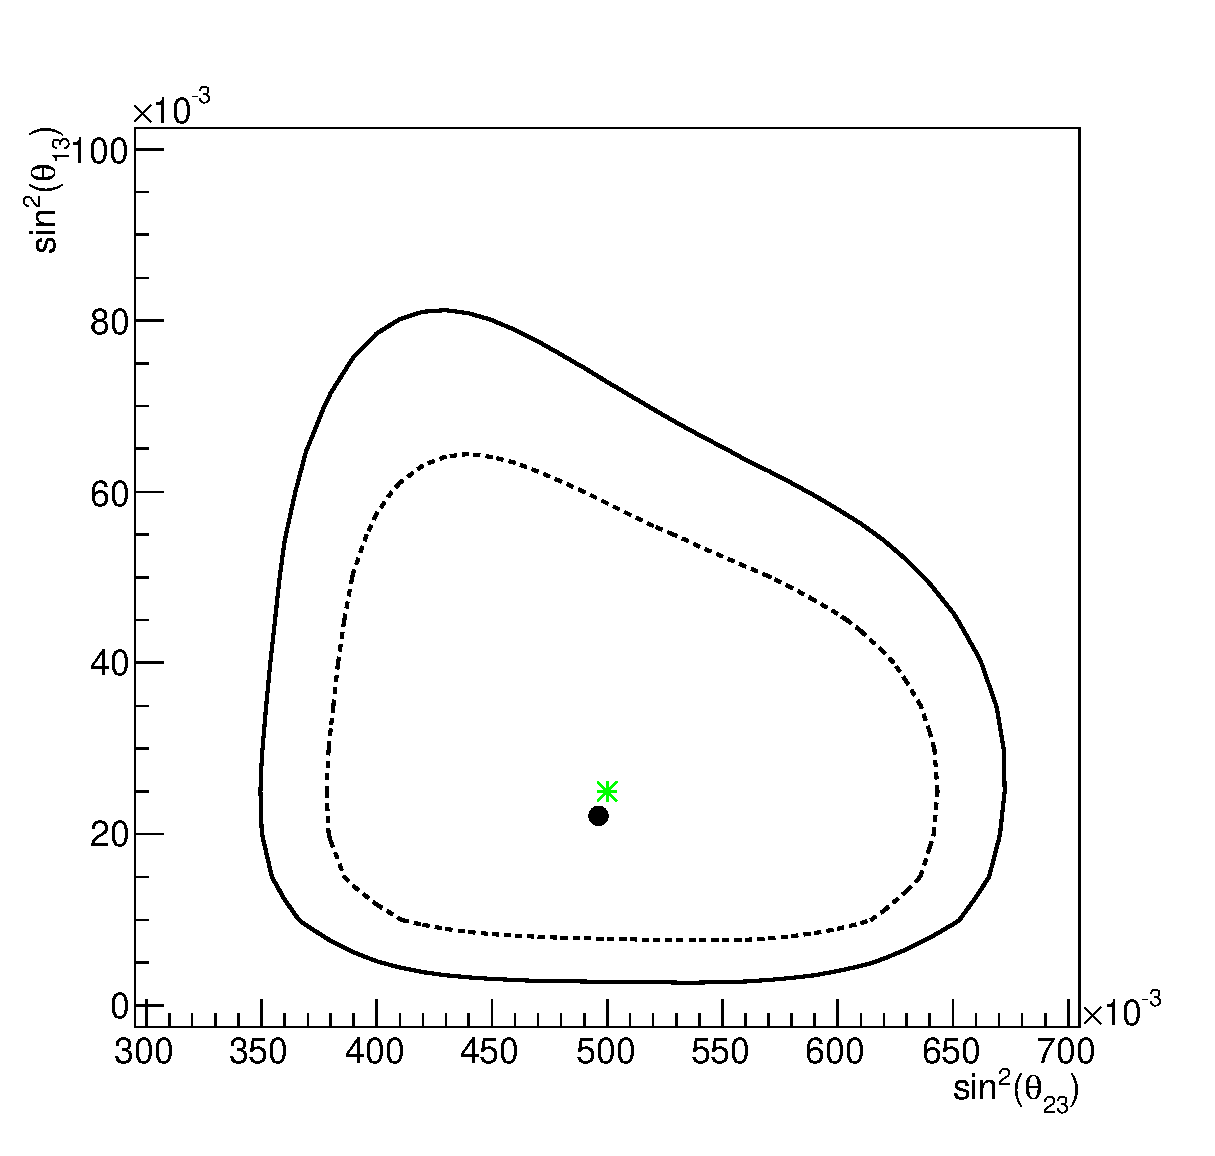
\includegraphics[width=15pc]{./images/appendix/fake_dataset_fits/fake_dataset9_chisq_theta13_theta23_global_min_new.eps}
\caption {
  68\% and 90\% CL regions in ($sin^{2}\theta_{23}$, $sin^{2}\theta_{13}$) space for fake dataset \#5.
  At each point, $\chi^2$ was minimized with respect to 
  all oscillation parameters not shown (and not considered to be fixed)
  and all relevant nuisance parameters.
}
\label{fig:toymc5_confreg_sinsqtheta23_sinsqtheta13}
\end{minipage}

\end{figure*}


\clearpage


%%%%%%%%%%%%%%%%%%%%%%%%%%%%%%%%%%%%%%%%%%%%%%%%%%%%%%%%%%%%%%%%
%%%%%%%%%%%%%%%%%%%%%%%%%%%%%%%%%%%%%%%%%%%%%%%%%%%%%%%%%%%%%%%%
%%%%%%%%%%%% REALISTIC FAKE DATASETS %%%%%%%%%%%%%%%%%%%%%%%%%%%%%%%%%%%%%
%%%%%%%%%%%%%%%%%%%%%%%%%%%%%%%%%%%%%%%%%%%%%%%%%%%%%%%%%%%%%%%%



\begin{sidewaystable}[htb]
\small
\centering
\begin{tabular}{@{}|p{0.1cm}p{2.5cm}|p{1.5cm}p{1cm}p{1cm}p{1cm}|p{1cm}|p{1.0cm}p{1.0cm}|p{1.2cm}p{1.2cm}|p{1.5cm}|@{}}
\hline
Set &   & $|\Delta m^2|$  & sin$^2\theta_{23}$ & sin$^2\theta_{13}$  & $\delta_{CP}$  &  MH & N$_{SK}^{1R\mu}$ & N$_{SK}^{1Re}$ & $\chi^2$/ndf & p-value & Systematics \\
 &   & ( $\times$10$^{-3}$ eV$^{2}$/c$^{4}$) &  &   &  &   &  & &  & &  \\
\hline
6  & true                      & {\bf 2.36 }   & {\bf 0.5}   & {\bf 0.025}   & {\bf 0.0}  & {\bf Normal} & {\bf 63 }   & {\bf 7}    & --        & --   & {\bf Nominal} \\
   & fit (joint)               &    2.369       &  0.509     &   0.016    &   2.110 & (fixed)    &   60.887   &   6.752    &  81.85/94          & 0.95  & See Fig. \ref{fig:toymc6_1Rmu_bestfit_spectrum} -  \\
   & fit ($\nu_{e}$ app.)      & --                             & --         &   0.011    & 0(fixed)  &     & --         &     6.741  &    16.98/24     & 0.98 &  \ref{fig:toymc6_confreg_sinsqtheta23_sinsqtheta13} \\
   & fit ($\nu_{\mu}$ disapp.) &    2.356      &   0.514    & --         & --       &   &   61.010    & --          & 65.09/71    &  0.81 &   \\
\hline
7  & true                      & {\bf 2.36 }   & {\bf 0.5}   & {\bf 0.025}   & {\bf 0.0}  & {\bf Normal} & {\bf 55}   & {\bf 11}    & --          & --   & {\bf Random} \\
   & fit (joint)               &     2.511      &    0.516   &    0.030   &   0.722 & (fixed)    &    54.802  &     10.962  & 73.86/94        & 0.35  & See Fig. \ref{fig:toymc7_1Rmu_bestfit_spectrum} -  \\
   & fit ($\nu_{e}$ app.)      & --                             & --         &    0.026   & 0(fixed)  &     & --         &   10.894    & 22.70/24      & 0.20 &   \ref{fig:toymc7_confreg_sinsqtheta23_sinsqtheta13}\\
   & fit ($\nu_{\mu}$ disapp.) &   2.492       &     0.514  & --         & --       &    &55.406       & --          & 52.24/71    &  0.53  &   \\
   \hline
8  & true                      & {\bf 2.36 }   & {\bf 0.5}   & {\bf 0.025}   & {\bf 0.0}  & {\bf Normal} & {\bf 55}   & {\bf 12}    & --          & --   & {\bf $E_{reco}$ scale: -1$\sigma$} \\
   & fit (joint)               &    2.431       &  0.520     &     0.036  &   0.707 & (fixed)    &    56.166  &  12.679     & 74.34/94        & 0.17  & See Fig. \ref{fig:toymc8_1Rmu_bestfit_spectrum} -  \\
   & fit ($\nu_{e}$ app.)      & --                             & --         &   0.032    & 0(fixed)  &     & --         &  12.695     & 16.65/24      & 0.39 &   \ref{fig:toymc8_confreg_sinsqtheta23_sinsqtheta13}\\
   & fit ($\nu_{\mu}$ disapp.) &     2.431     &    0.514   & --         & --       &    &  56.821     & --          & 58.10/71    & 0.09 &   \\
\hline
9  & true                      & {\bf 2.36 }   & {\bf 0.38}   & {\bf 0.025}   & {\bf 0.0}  & {\bf Normal} & {\bf 53}   & {\bf 11}    & --          & --   & {\bf Nominal} \\
   & fit (joint)               &     2.317      &    0.400   &    0.030   &   -0.263 & (fixed)    &    61.157  &     11.138  & 101.18/94        & 0.73  & See Fig. \ref{fig:toymc9_1Rmu_bestfit_spectrum} -  \\
   & fit ($\nu_{e}$ app.)      & --                             & --         &    0.026   & 0(fixed)  &     & --         &   11.272    & 29.70/24      & 0.71 &   \ref{fig:toymc9_confreg_sinsqtheta23_sinsqtheta13}\\
   & fit ($\nu_{\mu}$ disapp.) &   2.278       &     0.403  & --         & --       &    & 60.964       & --          & 72.07/71    & 0.49 &   \\
   \hline
10  & true                      & {\bf 2.36 }   & {\bf 0.5}   & {\bf 0.015}   & {\bf 0.0}  & {\bf Normal} & {\bf 57}   & {\bf 5}    & --          & --   & {\bf Nominal} \\
   & fit (joint)               &     2.427      &    0.505   &    0.009   &   1.072 & (fixed)    &    56.061  &     5.087  & 78.51/94        & 0.30  & See Fig. \ref{fig:toymc10_1Rmu_bestfit_spectrum} -  \\
   & fit ($\nu_{e}$ app.)      & --                             & --         &    0.006   & 0(fixed)  &     & --         &   5.047    & 17.13/24      & 0.43 &   \ref{fig:toymc10_confreg_sinsqtheta23_sinsqtheta13}\\
   & fit ($\nu_{\mu}$ disapp.) &   2.420       &     0.514  & --         & --       &    & 56.235       & --          & 62.16/71    & 0.27 &   \\
   \hline
11  & true                      & {\bf 2.36 }   & {\bf 0.5}   & {\bf 0.025}   & {\bf -$\pi/2$}  & {\bf Normal} & {\bf 69}   & {\bf 13}    & --          & --   & {\bf Nominal} \\
   & fit (joint)               &     2.455      &    0.389   &    0.048   &   0.706 & (fixed)    &    68.012  &     12.594  & 75.27/94        & 0.25 & See Fig. \ref{fig:toymc11_1Rmu_bestfit_spectrum} -  \\
   & fit ($\nu_{e}$ app.)      & --                             & --         &    0.031   & 0(fixed)  &     & --         &   12.541    & 24.58/24      & 0.08 &   \ref{fig:toymc11_confreg_sinsqtheta23_sinsqtheta13}\\
   & fit ($\nu_{\mu}$ disapp.) &   2.411       &     0.384  & --         & --       &    & 68.452       & --          & 50.88/71    & 0.80 &   \\
   \hline
12  & true                      & {\bf 2.2 }   & {\bf 0.5}   & {\bf 0.025}   & {\bf 0.0}  & {\bf Normal} & {\bf 53}   & {\bf 7}    & --          & --   & {\bf Nominal} \\
   & fit (joint)               &     2.234      &    0.506   &    0.013   &   3.141 & (fixed)    &    57.620  &     6.972  & 90.38/94        & 0.93  & See Fig. \ref{fig:toymc12_1Rmu_bestfit_spectrum} -  \\
   & fit ($\nu_{e}$ app.)      & --                             & --         &    0.012   & 0(fixed)  &     & --         &   6.961    & 18.67/24      & 0.85 &   \ref{fig:toymc12_confreg_sinsqtheta23_sinsqtheta13}\\
   & fit ($\nu_{\mu}$ disapp.) &   2.220       &     0.513  & --         & --       &    & 57.665       & --          & 72.36/71    & 0.76 &   \\
     \hline
13  & true                      & {\bf 2.36 }   & {\bf 0.5}   & {\bf 0.025}   & {\bf 0.0}  & {\bf Inverted} & {\bf 52}   & {\bf 11}    & --          & --   & {\bf Nominal} \\
   & fit (joint)               &     2.503      &    0.513   &    0.029   &   -0.379  & (fixed)    &    54.485  &     11.374  & 73.72/94        & 0.58  & See Fig. \ref{fig:toymc13_1Rmu_bestfit_spectrum} -  \\
   & fit ($\nu_{e}$ app.)      & --                             & --         &    0.033   & 0(fixed)  &     & --         &   11.450    & 15.82/24      & 0.60 &   \ref{fig:toymc13_confreg_sinsqtheta23_sinsqtheta13}\\
   & fit ($\nu_{\mu}$ disapp.) &   2.513       &     0.511  & --         & --       &    & 54.708       & --          & 58.09/71    & 0.53 &   \\


\hline
\end{tabular}
\caption{
  True input values (shown in bold) and VALOR best-fit values for a test ensemble of 7 fake datasets with statistical fluctuations
}
\label{tab:toymc_fits:best_fit_values_realistic}
\end{sidewaystable}

\clearpage
% 
% 
% ..............................................
% Fake dataset #6 
% 
%

%
% best-fit spectra and pulls
%

\begin{figure*}[htb]

\begin{minipage}[t]{0.46\linewidth}
\center
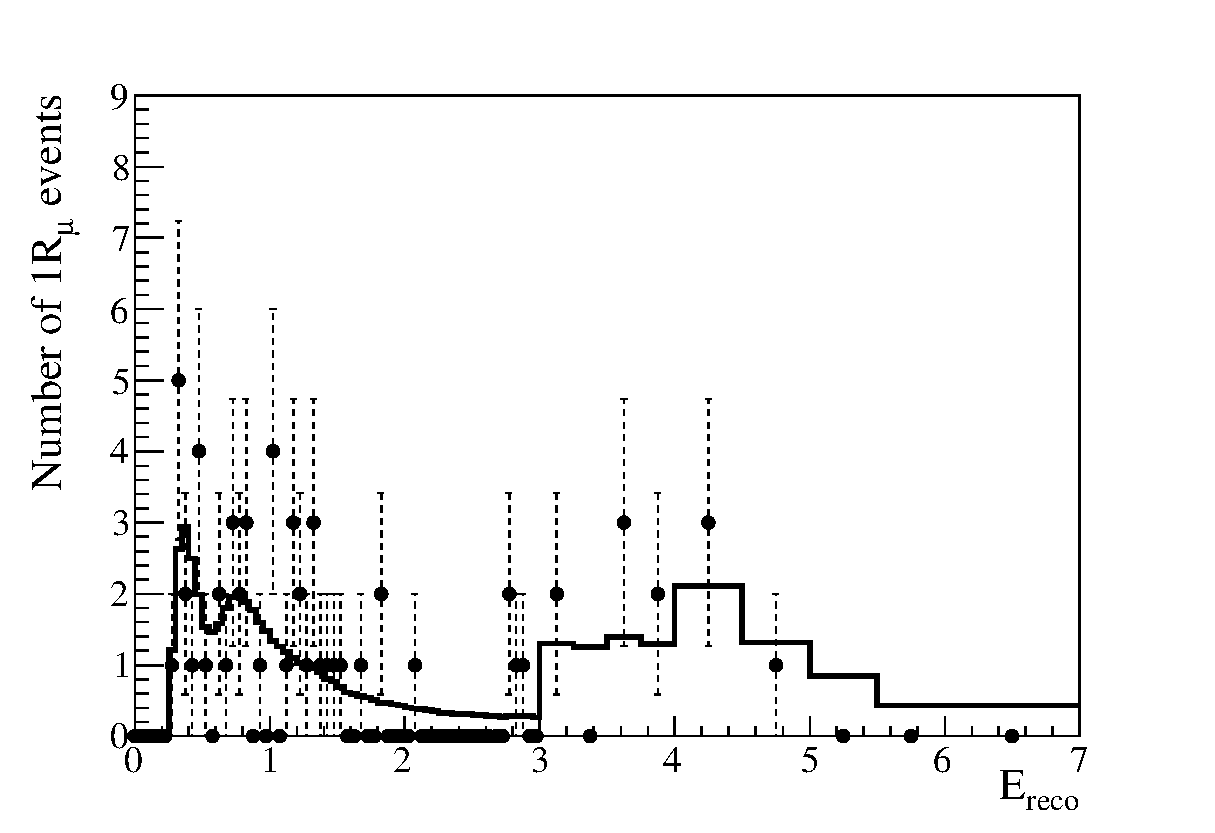
\includegraphics[width=15pc]{./images/appendix/fake_dataset_fits/realistic_fake_dataset0_nh_1st_1Rmu.eps}
\caption {
  Single $\mu$-like ring event best-fit reconstructed energy spectrum
  to fake dataset \#6.
}
\label{fig:toymc6_1Rmu_bestfit_spectrum}
\end{minipage}
\hspace{0.03\linewidth}
\begin{minipage}[t]{0.46\linewidth}
\center
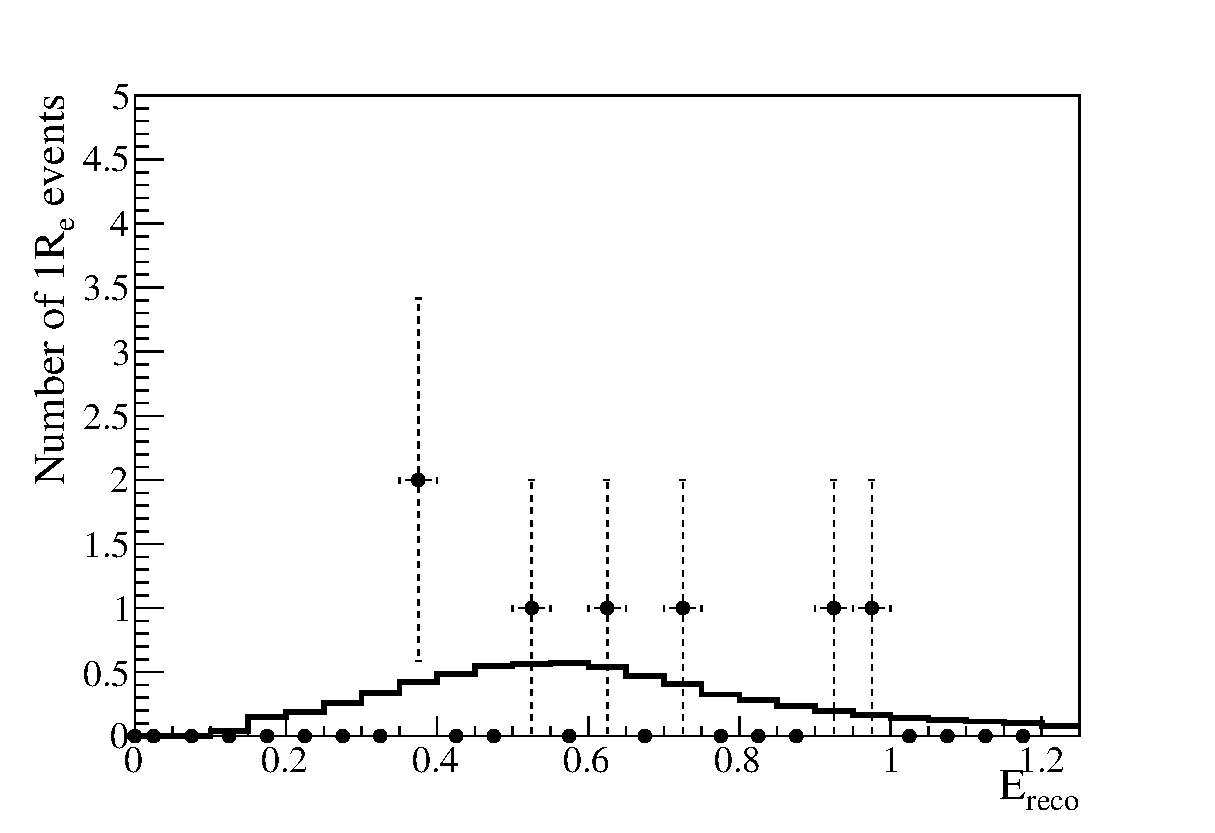
\includegraphics[width=15pc]{./images/appendix/fake_dataset_fits/realistic_fake_dataset0_nh_1st_1Re.eps}
\caption {
  Single e-like ring event best-fit reconstructed energy spectrum
  to fake dataset \#6.
}
\label{fig:toymc6_1Re_bestfit_spectrum}
\end{minipage}

\vfill
\vspace*{0.7cm}

\begin{minipage}[t]{0.90\linewidth}
\center
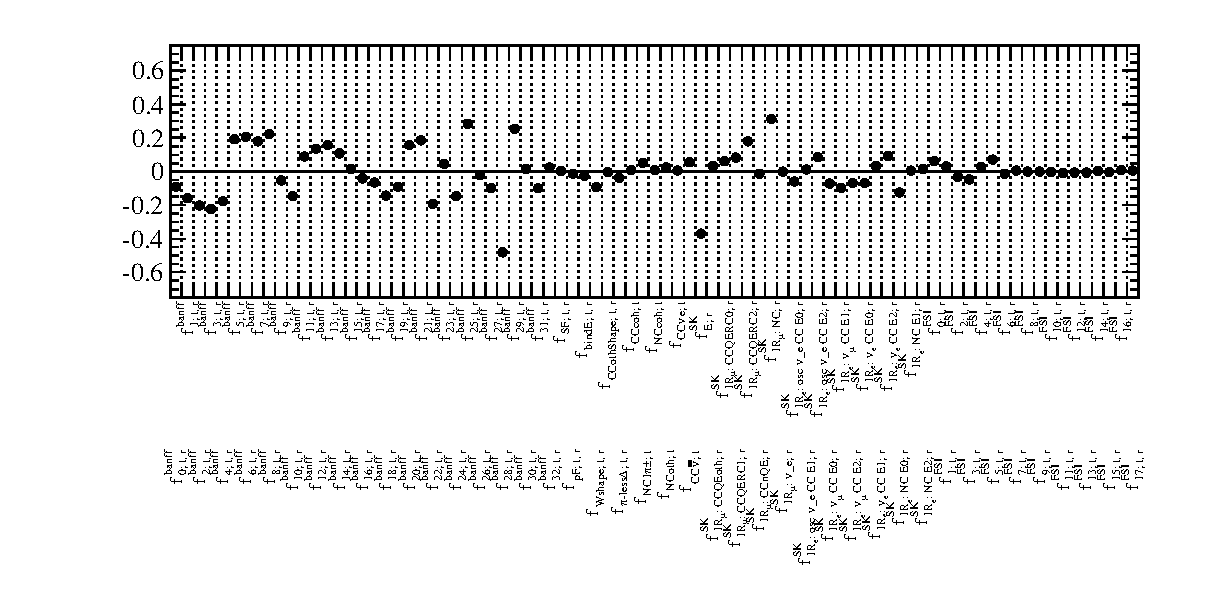
\includegraphics[width=30pc,angle=270]{./images/appendix/fake_dataset_fits/pulls_realistic_fake_dataset0_nh_1st.eps}
\caption {
  Systematic parameter pulls for the oscillation fit to fake dataset \#6.
}
\label{fig:toymc6_pulls}
\end{minipage}

\end{figure*}

\clearpage


%...........................................................
%
% chisq distributions used for calculating the fit p-values
%

\begin{figure*}[htb]

\begin{minipage}[t]{0.90\linewidth}
\center
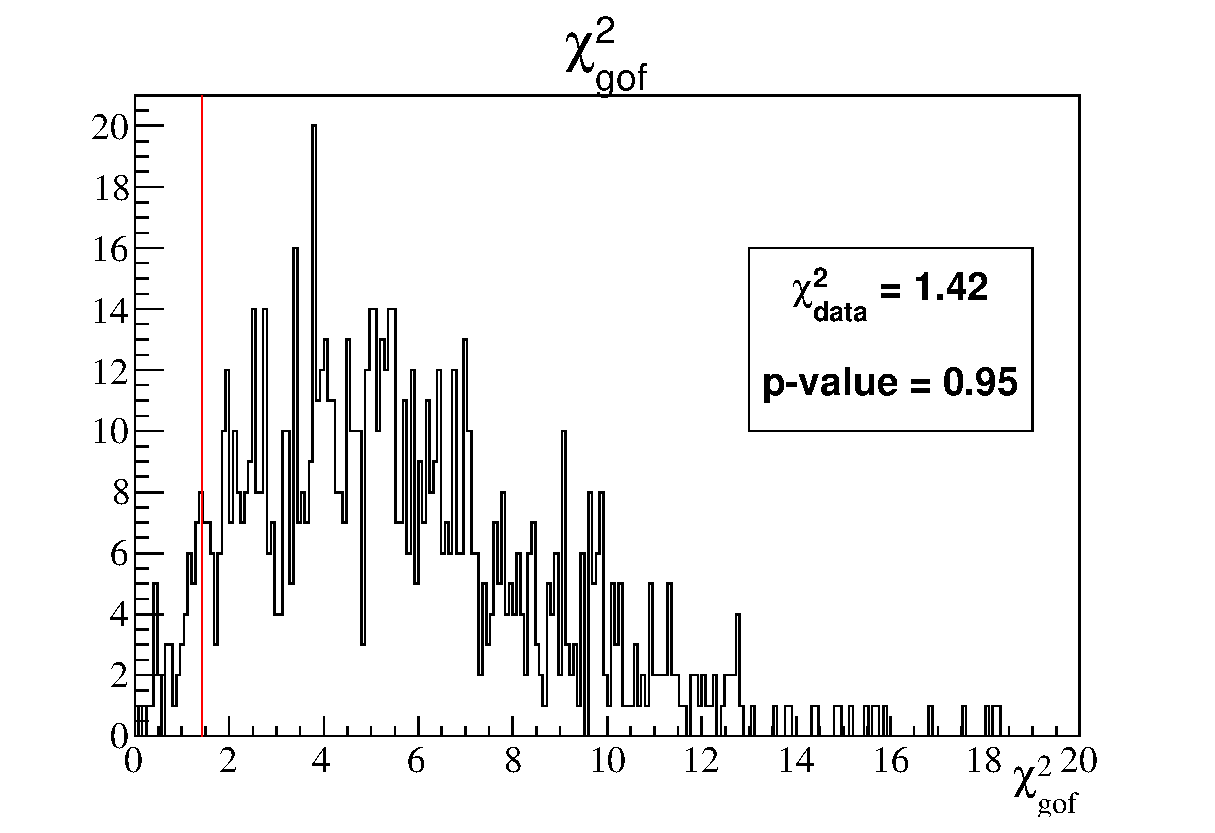
\includegraphics[width=30pc]{./images/appendix/fake_dataset_fits/realistic_fake_dataset0_nh_1st_gof_new.eps}
\caption {
  Distribution of $\chi^2_{gof}$, the goodness-of-fit (gof) $\chi^2$, 
  from 1k toy MC experiments generated at dataset \#6 joint 3-flavour analysis best-fit oscillation point.
  The $\chi^2_{gof}$ value for the dataset \#6 ($\chi^2_{data}$) is highlighted.
  All $\chi^2_{gof}$ values were computed 
  using the 5 (single $\mu$-like ring) + 1 (single e-like ring) 
  reconstructed energy binning scheme described in Sec.\ \ref{sec:goodness_of_fit},
}
\label{fig:toymc6_gofchisq}
\end{minipage}

\vfill
\vspace*{0.7cm}

\begin{minipage}[t]{0.46\linewidth}
\center
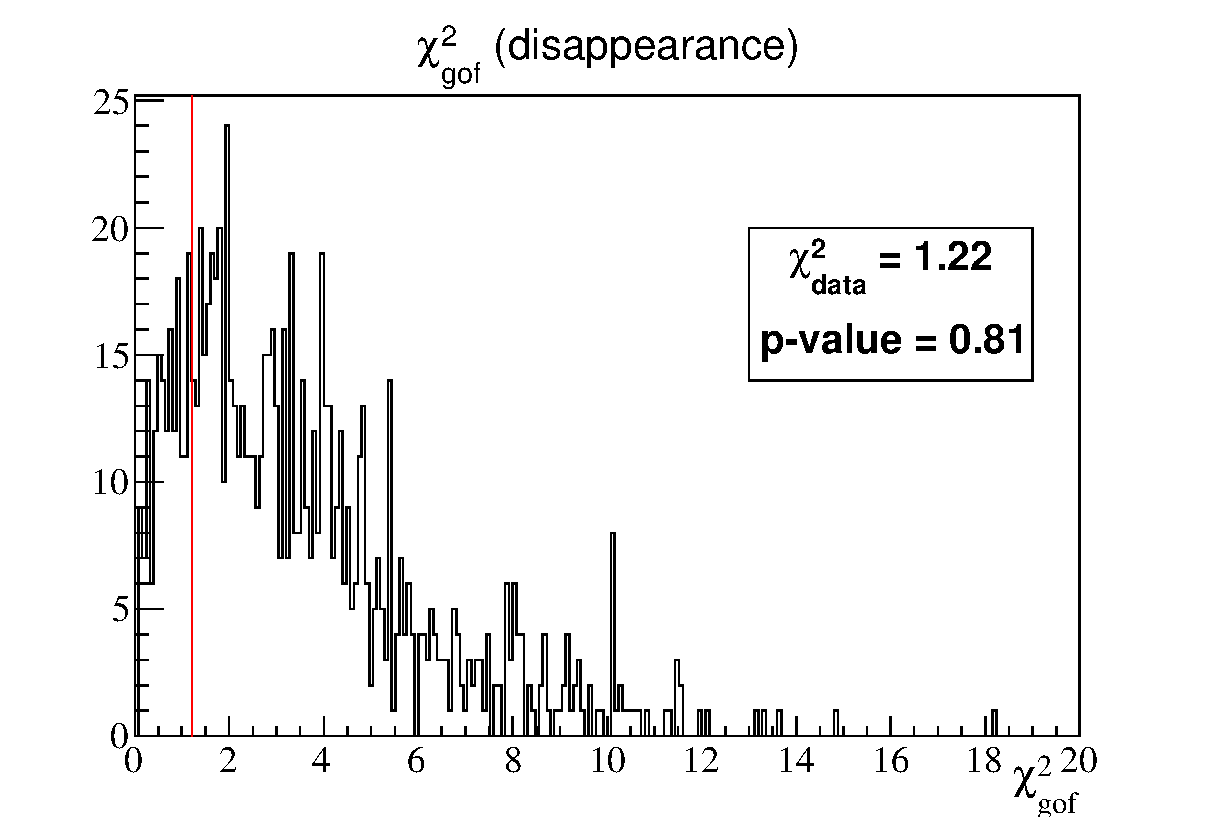
\includegraphics[width=18pc]{./images/appendix/fake_dataset_fits/realistic_fake_dataset0_nh_1st_gof_disap_new.eps}
\caption {
  Distribution of $\chi^2_{gof}$
  from 1k toy MC experiments generated at the dataset \#6 stand-alone 3-flavour $\nu_{\mu}$ disappearance analysis best-fit oscillation point.
  The $\chi^2_{gof}$ value for the dataset \#6 ($\chi^2_{data}$) is highlighted.
  All $\chi^2_{gof}$ values were computed 
  using the 5 (single $\mu$-like ring) 
  reconstructed energy binning scheme described in Sec.\ \ref{sec:goodness_of_fit},
}
\label{fig:toymc6_gofchisq_disapp}
\end{minipage}
\hspace{0.03\linewidth}
\begin{minipage}[t]{0.46\linewidth}
\center
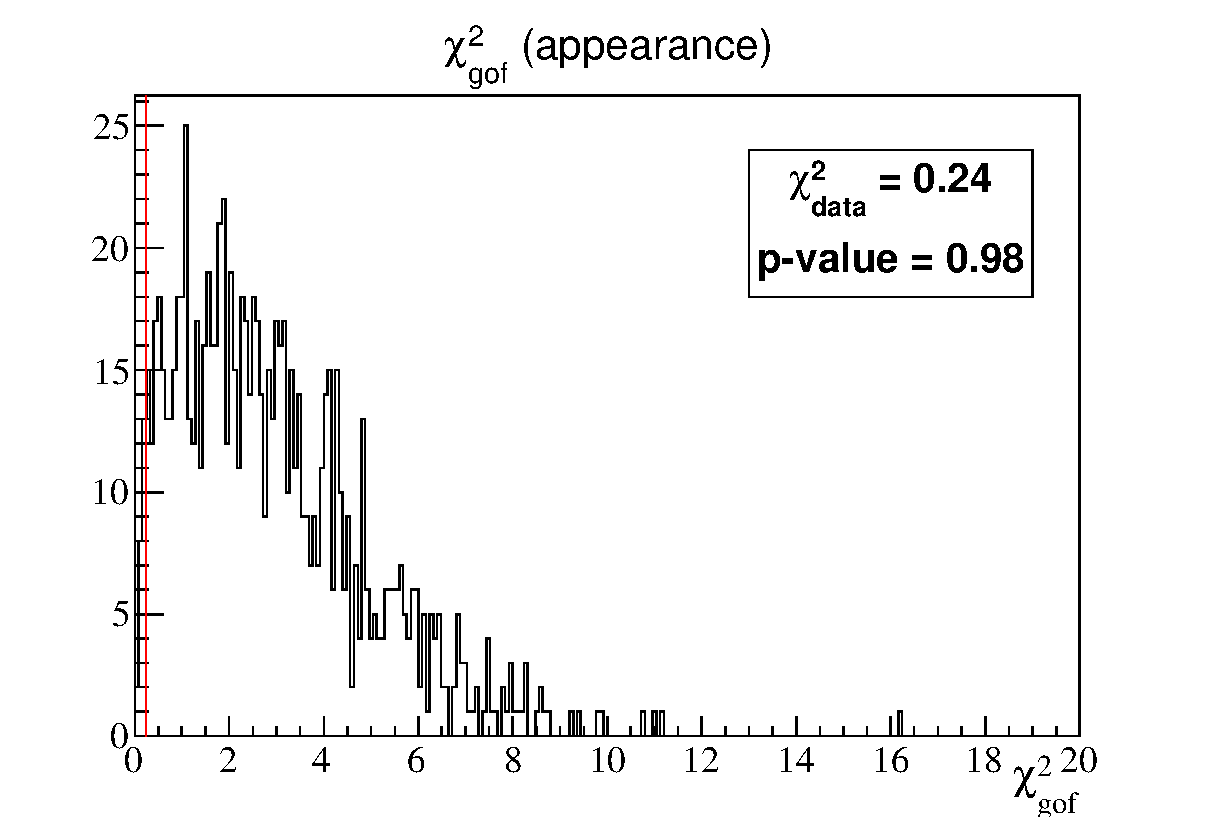
\includegraphics[width=18pc]{./images/appendix/fake_dataset_fits/realistic_fake_dataset0_nh_1st_gof_app_new.eps}
\caption {
  Distribution of $\chi^2_{gof}$
  from 1k toy MC experiments generated at the dataset \#6 stand-alone 3-flavour $\nu_{e}$ appearance analysis best-fit oscillation point.
  The $\chi^2_{gof}$ value for the dataset \#6 ($\chi^2_{data}$) is highlighted.
  All $\chi^2_{gof}$ values were computed 
  using a single reconstructed energy bin, as described in Sec.\ \ref{sec:goodness_of_fit},
}
\label{fig:toymc6_gofchisq_app}
\end{minipage}

\end{figure*}



%
% delta\chisq and contours
%

\begin{figure*}[htb]

\begin{minipage}[t]{0.22\linewidth}
\center
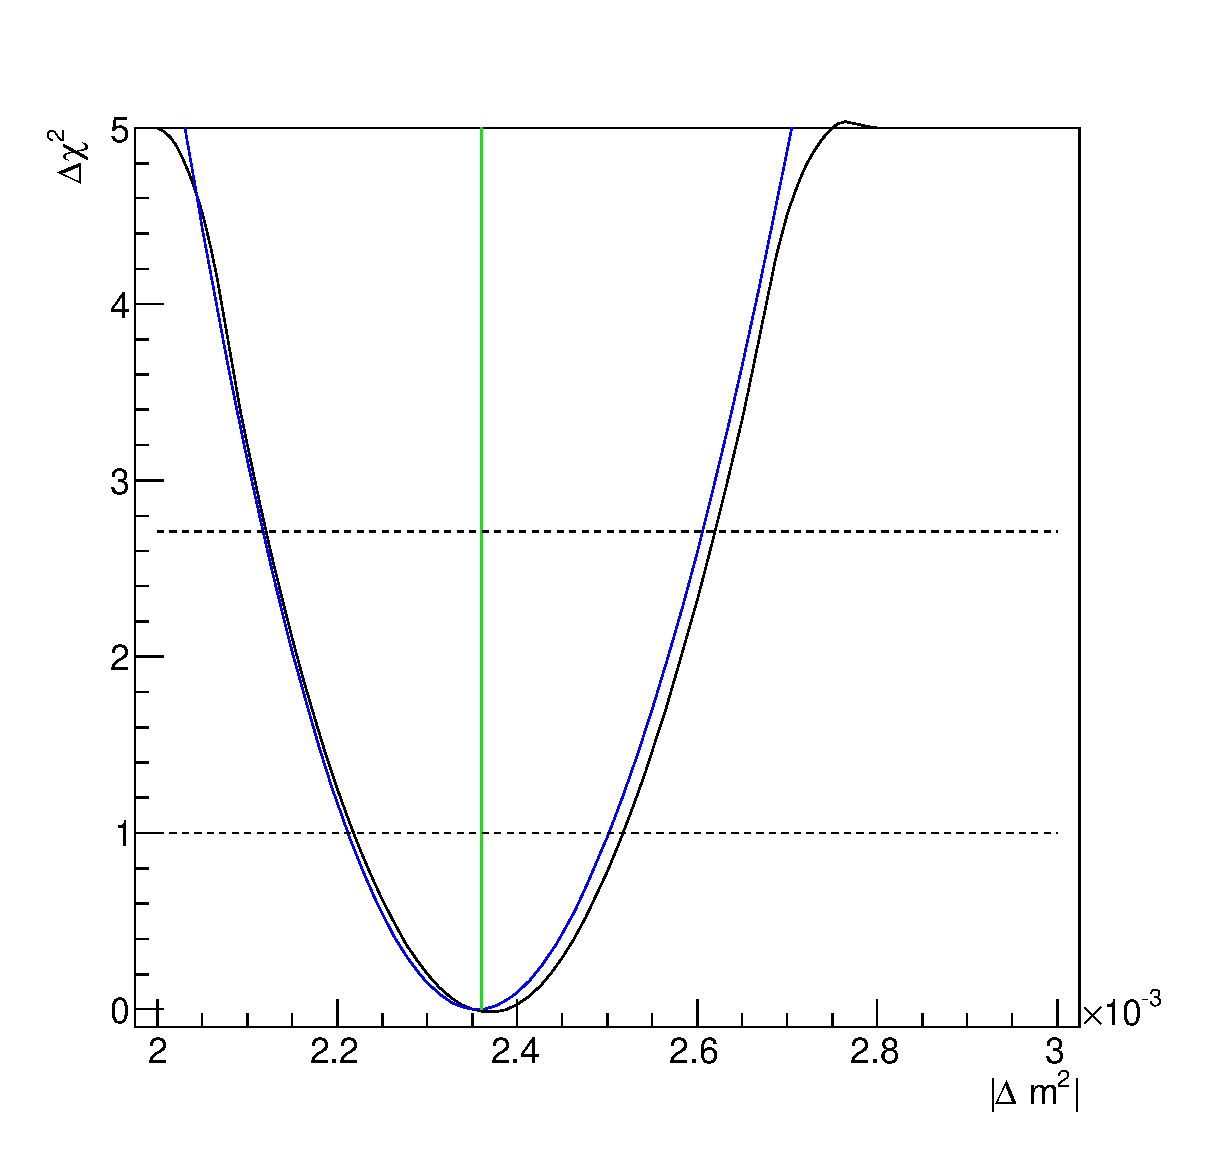
\includegraphics[width=9pc]{./images/appendix/fake_dataset_fits/realistic_fake_dataset0_chisq_dm23sq_global_min.eps}
\caption {
  $\Delta\chi^2$ as function of $|\Delta m^{2}|$ for fake dataset \#6.
  At each point, $\chi^2$ was minimized with respect to 
  $\sin^{2}\theta_{23}$, $\sin^{2}\theta_{13}$, $\delta_{CP}$
  and all relevant nuisance parameters for the joint analysis (black)
  and with respect to $\sin^{2}\theta_{23}$ and all relevant nuisance
  parameters for the disappearance analysis (blue).
}
\label{fig:toymc6_dchisq_Dmsq}
\end{minipage}
\hspace{0.02\linewidth}
\begin{minipage}[t]{0.22\linewidth}
\center
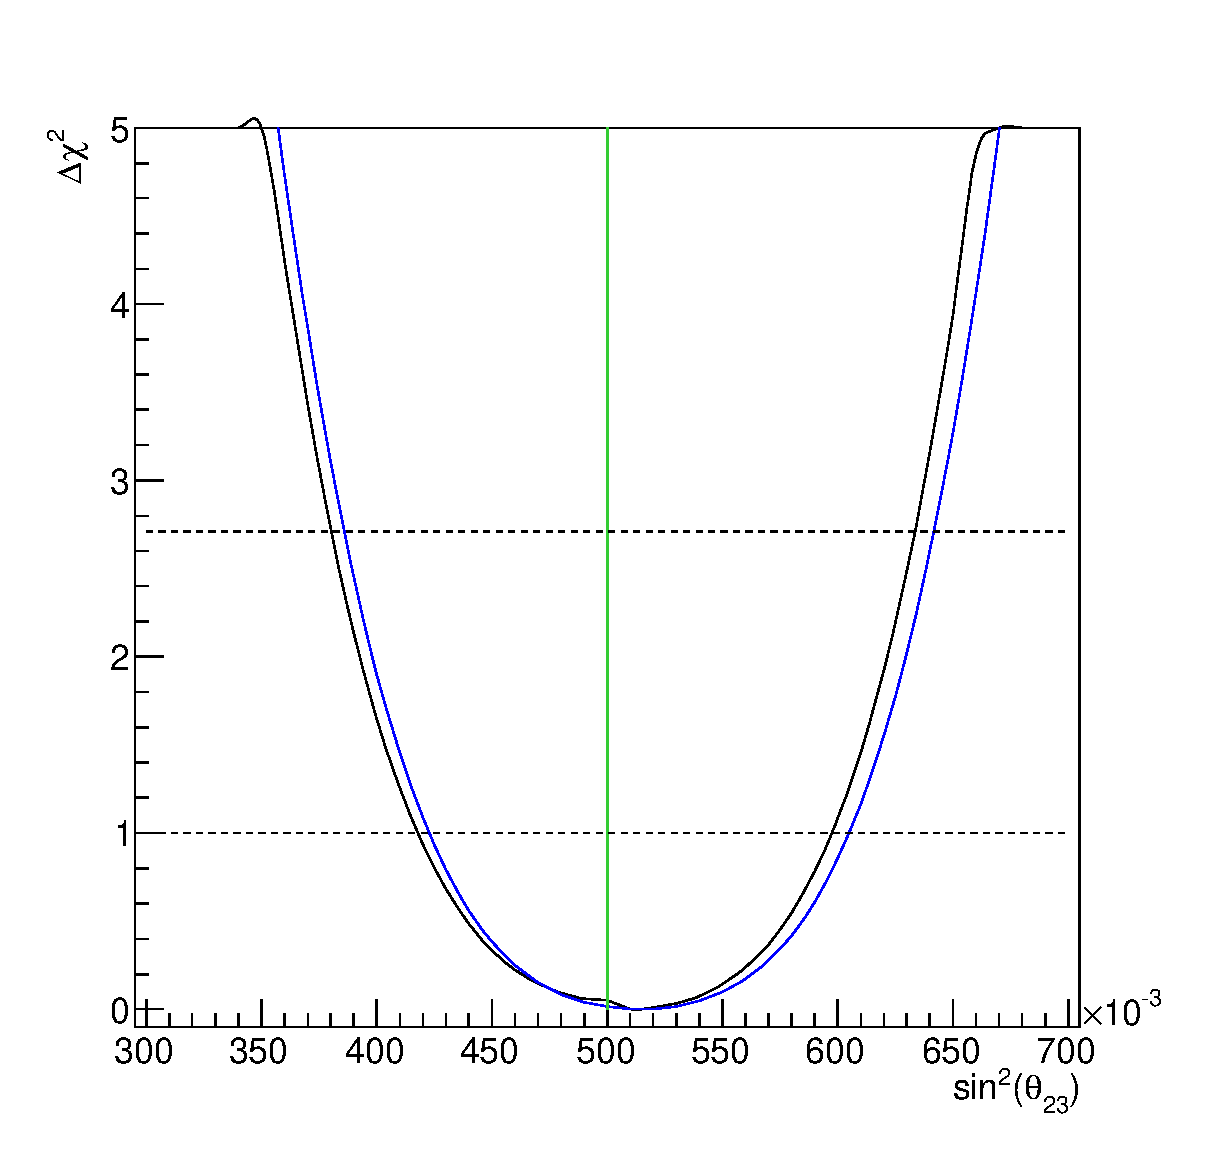
\includegraphics[width=9pc]{./images/appendix/fake_dataset_fits/realistic_fake_dataset0_chisq_theta23_global_min.eps}
\caption {
  $\Delta\chi^2$ as function of $sin^{2}\theta_{23}$ for fake dataset \#6.
  At each point, $\chi^2$ was minimized with respect to 
  $|\Delta m^{2}|$, $\sin^{2}\theta_{13}$, $\delta_{CP}$
  and all relevant nuisance parameters for the joint analysis (black)
  and with respect to $\sin^{2}\theta_{23}$ and all relevant nuisance
  parameters for the disappearance analysis (blue).
}
\label{fig:toymc6_dchisq_sinsqtheta23}
\end{minipage}
\hspace{0.02\linewidth}
\begin{minipage}[t]{0.22\linewidth}
\center
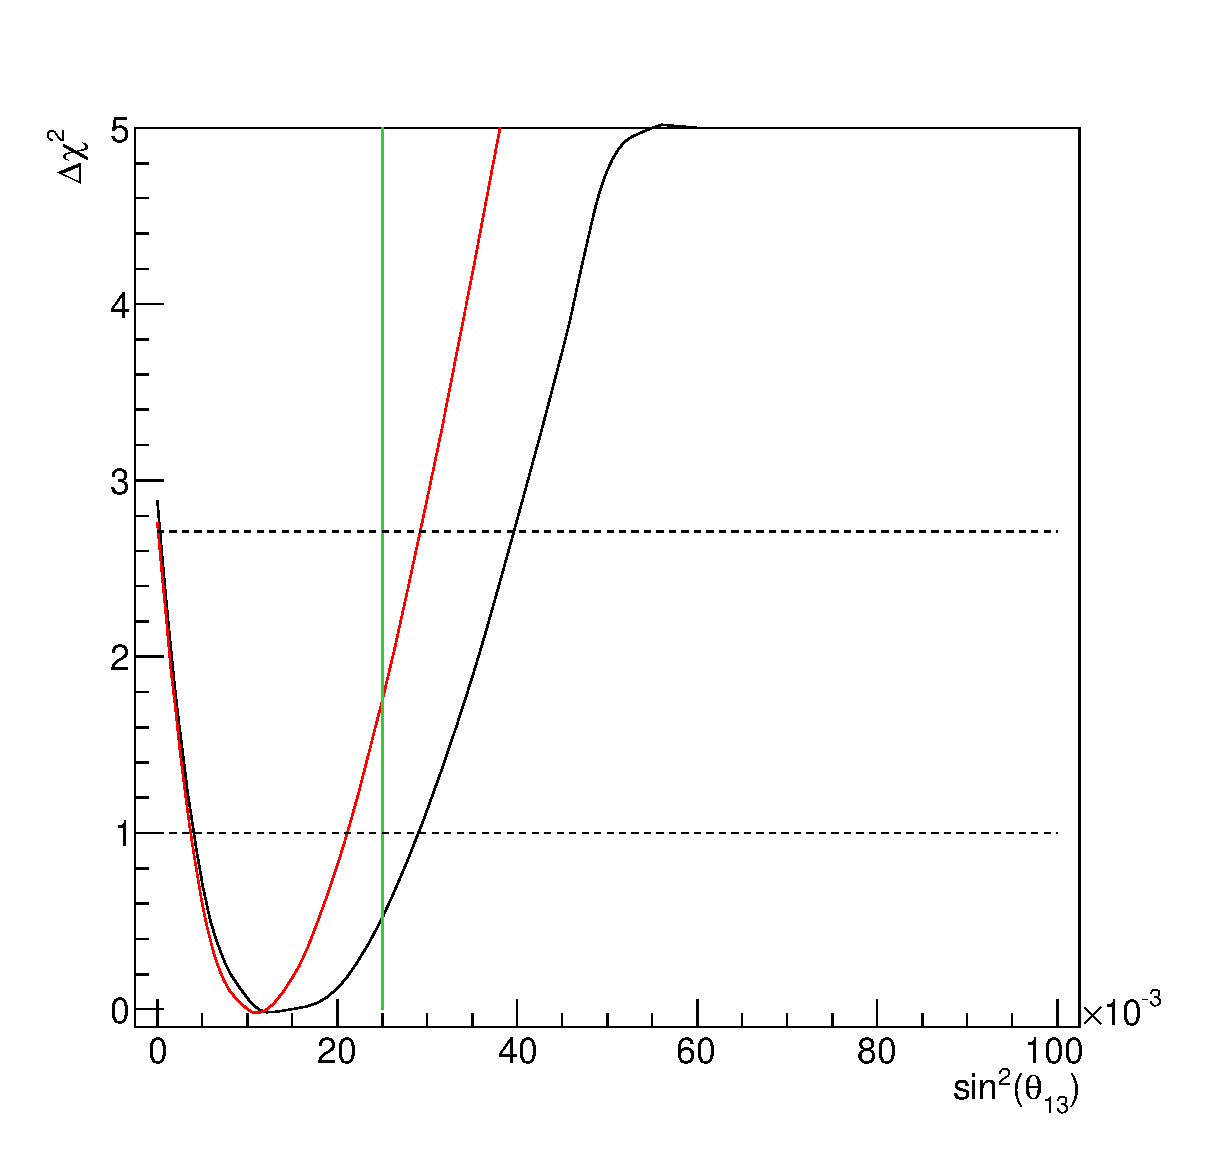
\includegraphics[width=9pc]{./images/appendix/fake_dataset_fits/realistic_fake_dataset0_chisq_theta13_global_min.eps}
\caption {
  $\Delta\chi^2$ as function of $sin^{2}\theta_{13}$ for fake dataset \#6.
  At each point, $\chi^2$ was minimized with respect to 
  $\sin^{2}\theta_{23}$, $\sin^{2}\theta_{13}$, $\delta_{CP}$
  and all relevant nuisance parameters for the joint analysis (black)
  and with respect to all relevant nuisance parameters 
  ($\delta_{CP}$ is fixed to 0) for the appearance analysis (red).
}
\label{fig:toymc6_dchisq_sinsqtheta13}
\end{minipage}
\hspace{0.02\linewidth}
\begin{minipage}[t]{0.22\linewidth}
\center
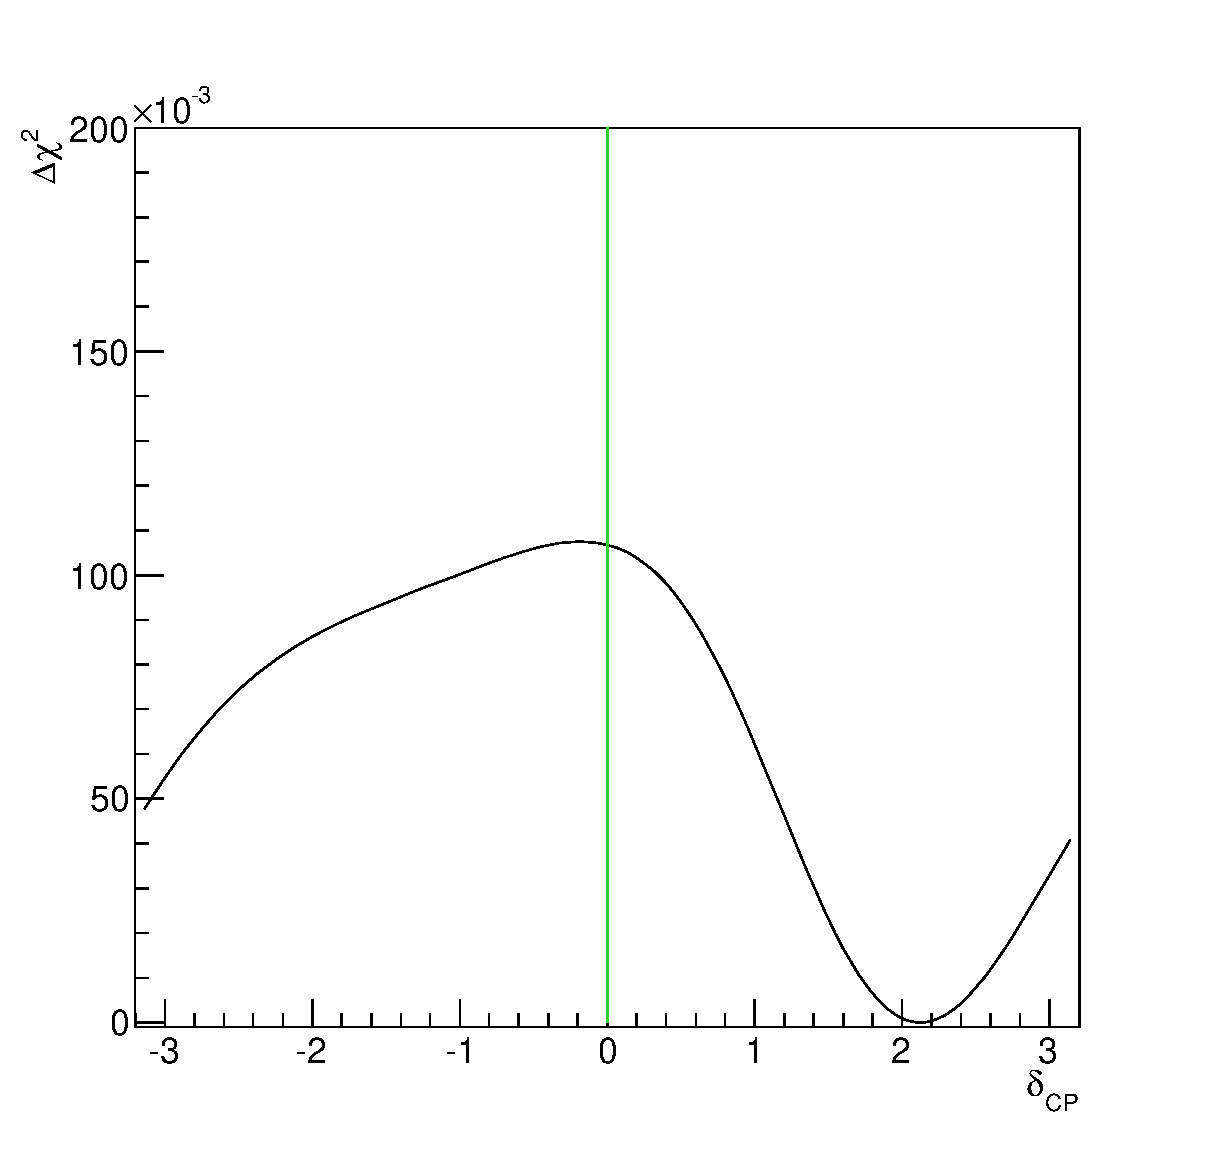
\includegraphics[width=9pc]{.//images/appendix/fake_dataset_fits/realistic_fake_dataset0_chisq_deltacp_global_min.eps}
\caption {
  $\Delta\chi^2$ as function of $\delta_{CP}$ for fake dataset \#6.
  At each point, $\chi^2$ was minimized with respect to 
  all oscillation parameters not shown (and not considered to be fixed)
  and all relevant nuisance parameters.
}
\label{fig:toymc6_dchisq_deltacp}
\end{minipage}
\vfill
\vspace*{0.7cm}
\begin{minipage}[t]{0.48\linewidth}
\center
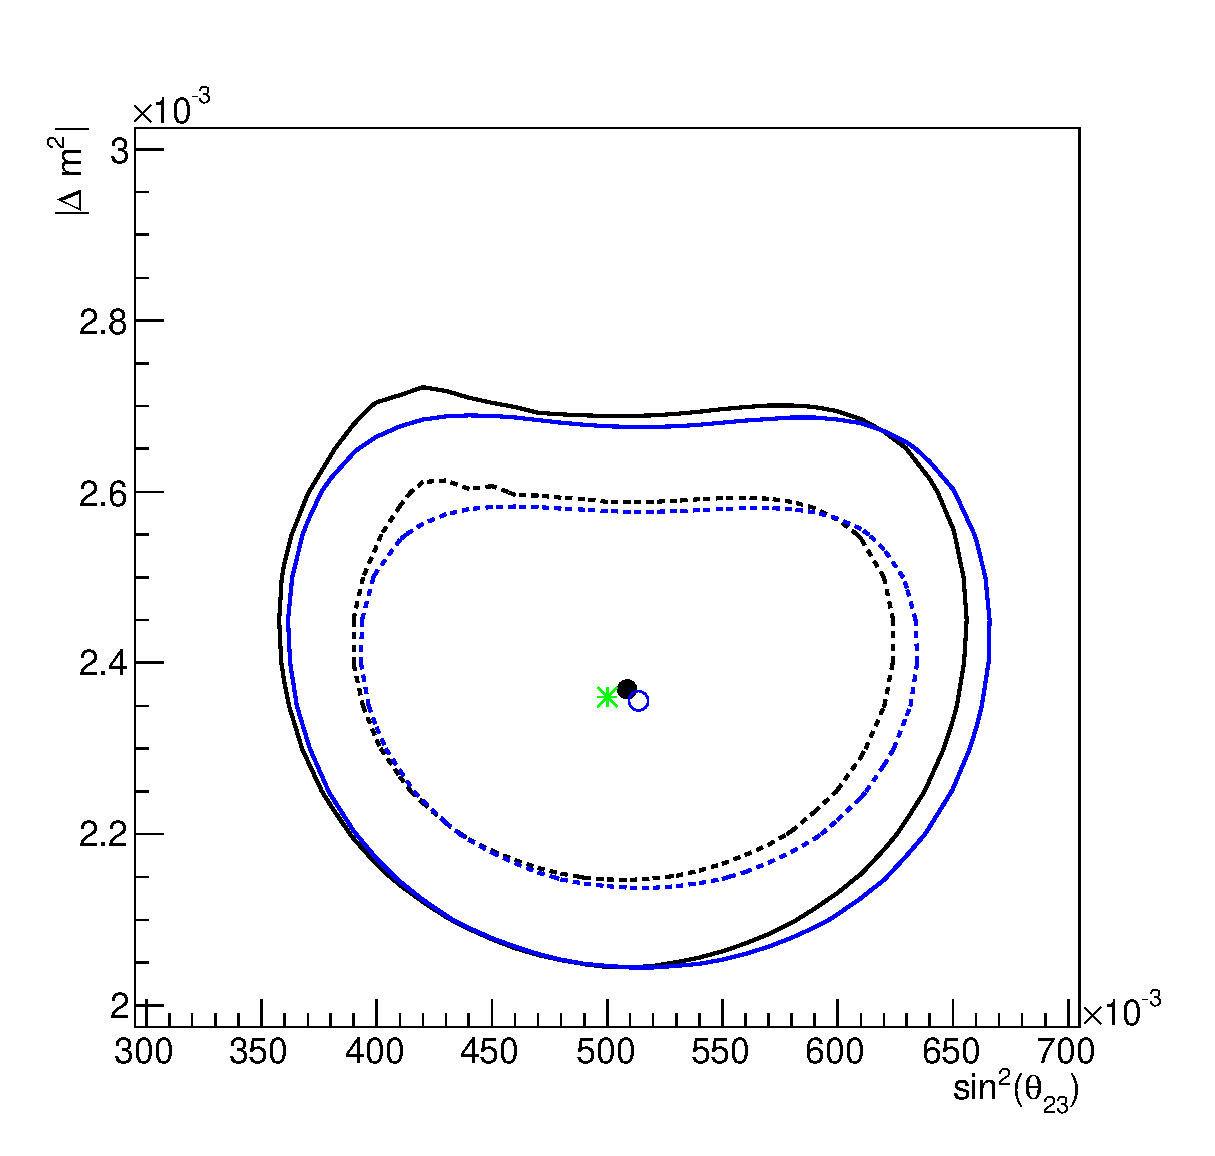
\includegraphics[width=15pc]{./images/appendix/fake_dataset_fits/realistic_fake_dataset0_chisq_theta23_dm23sq_global_min.eps}
\caption {
  68\% and 90\% CL regions in ($sin^{2}\theta_{23}$, $|\Delta m^{2}|$) space for fake dataset \#6.
  At each point, $\chi^2$ was minimized with respect to 
  $\sin^{2}\theta_{13}$, $\delta_{CP}$
  and all relevant nuisance parameters for the joint analysis (black)
  and with respect to all relevant nuisance parameters for the disappearance analysis (blue).
}
\label{fig:toymc6_confreg_sinsqtheta23_Dmsq}
\end{minipage}
\hspace{0.03\linewidth}
\begin{minipage}[t]{0.48\linewidth}
\center
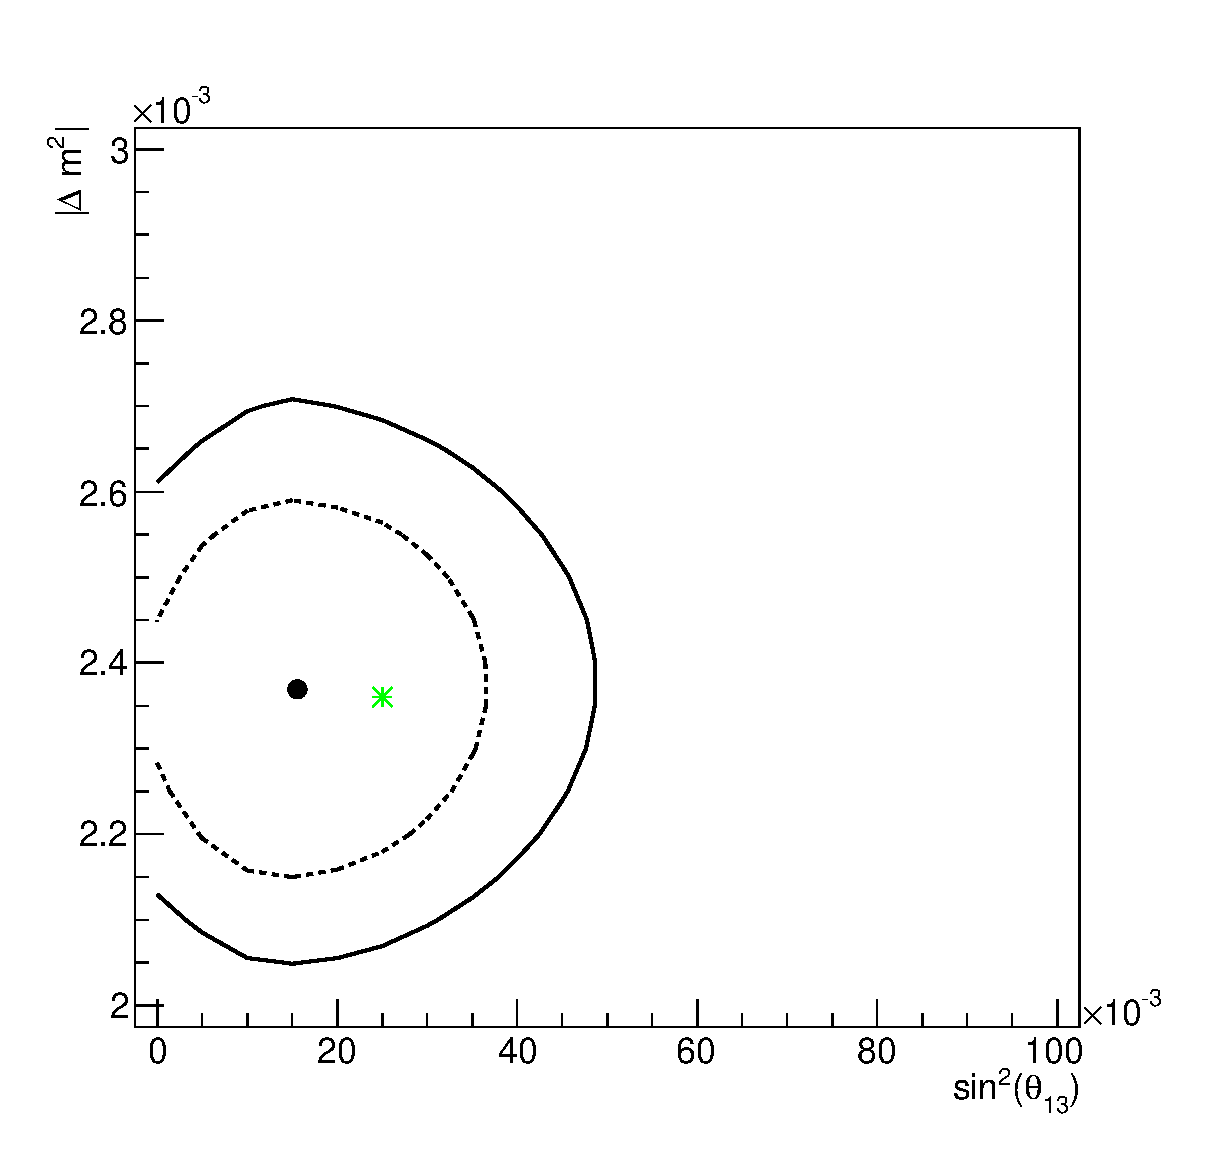
\includegraphics[width=15pc]{./images/appendix/fake_dataset_fits/realistic_fake_dataset0_chisq_theta13_dm23sq_global_min.eps}
\caption {
  68\% and 90\% CL regions in ($sin^{2}\theta_{13}$, $|\Delta m^{2}|$) space for fake dataset \#6.
  At each point, $\chi^2$ was minimized with respect to 
  all oscillation parameters not shown (and not considered to be fixed)
  and all relevant nuisance parameters.
}
\label{fig:toymc6_confreg_sinsqtheta13_Dmsq}
\end{minipage}

\vfill
\vspace*{0.7cm}

\begin{minipage}[t]{0.48\linewidth}
\center
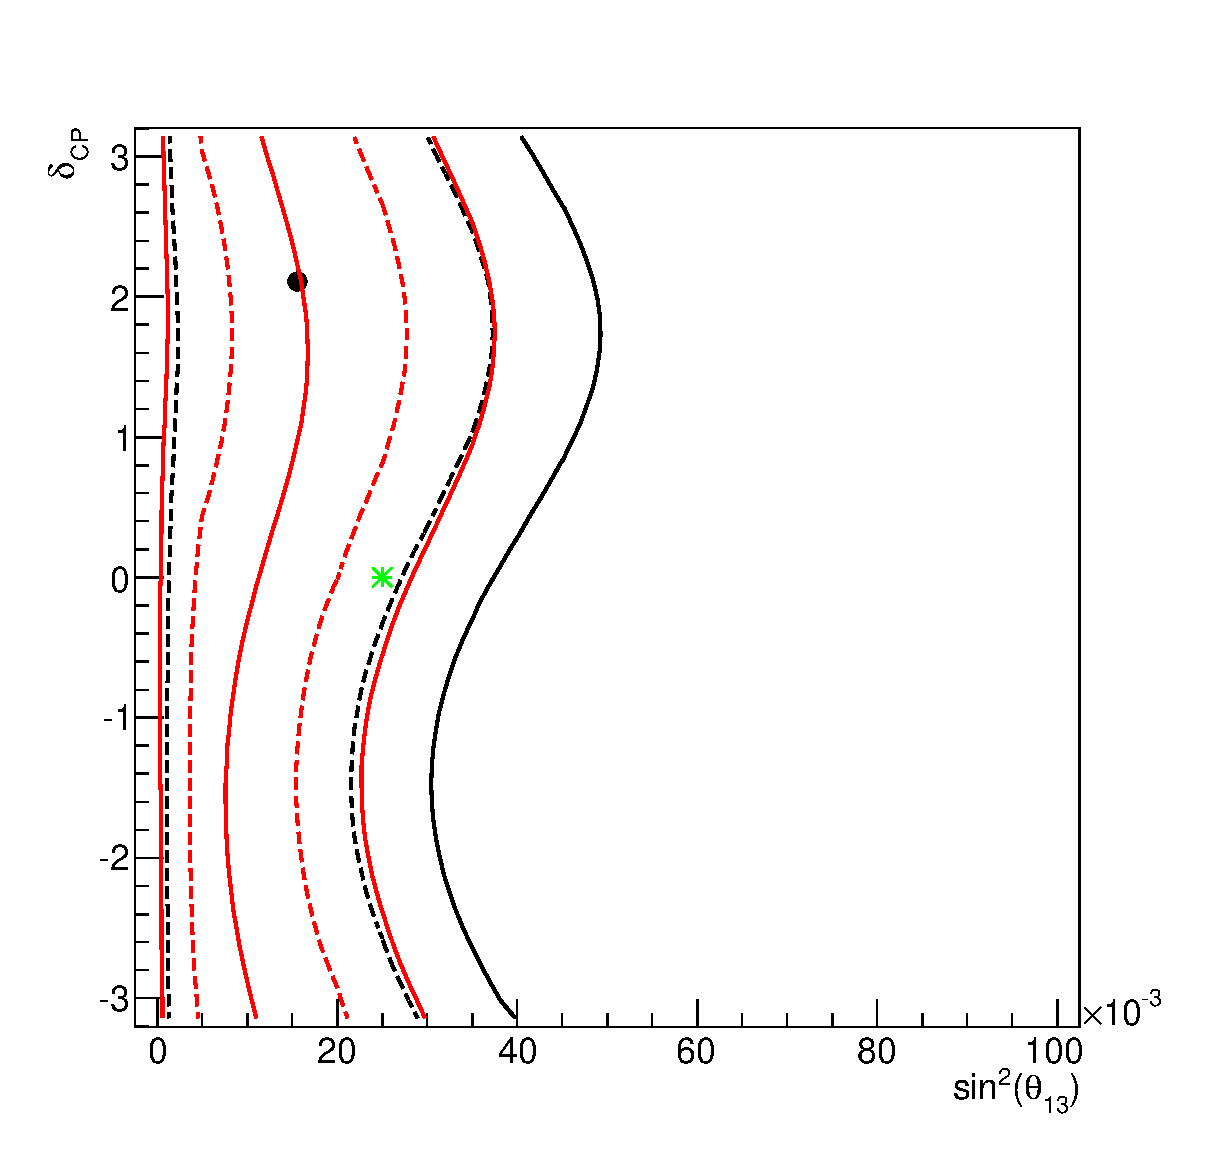
\includegraphics[width=15pc]{./images/appendix/fake_dataset_fits/realistic_fake_dataset0_chisq_theta13_deltacp_global_min.eps}
\caption {
  68\% and 90\% CL regions in ($sin^{2}\theta_{13}$, $\delta_{CP}$) space for fake dataset \#6.
  At each point, $\chi^2$ was minimized with respect to 
  $|\Delta m^{2}|$, $\sin^{2}\theta_{23}$
  and all relevant nuisance parameters for the joint analysis (black)
  and with respect to all relevant nuisance parameters for the appearance analysis (red).
  Notice that different methods are used to
  construct confidence regions for the joint analysis (global minimum) and for the 
  stand-alone appearance analysis (raster scan).
}
\label{fig:toymc6_confreg_sinsqtheta13_deltacp}
\end{minipage}
\hspace{0.03\linewidth}
\begin{minipage}[t]{0.48\linewidth}
\center
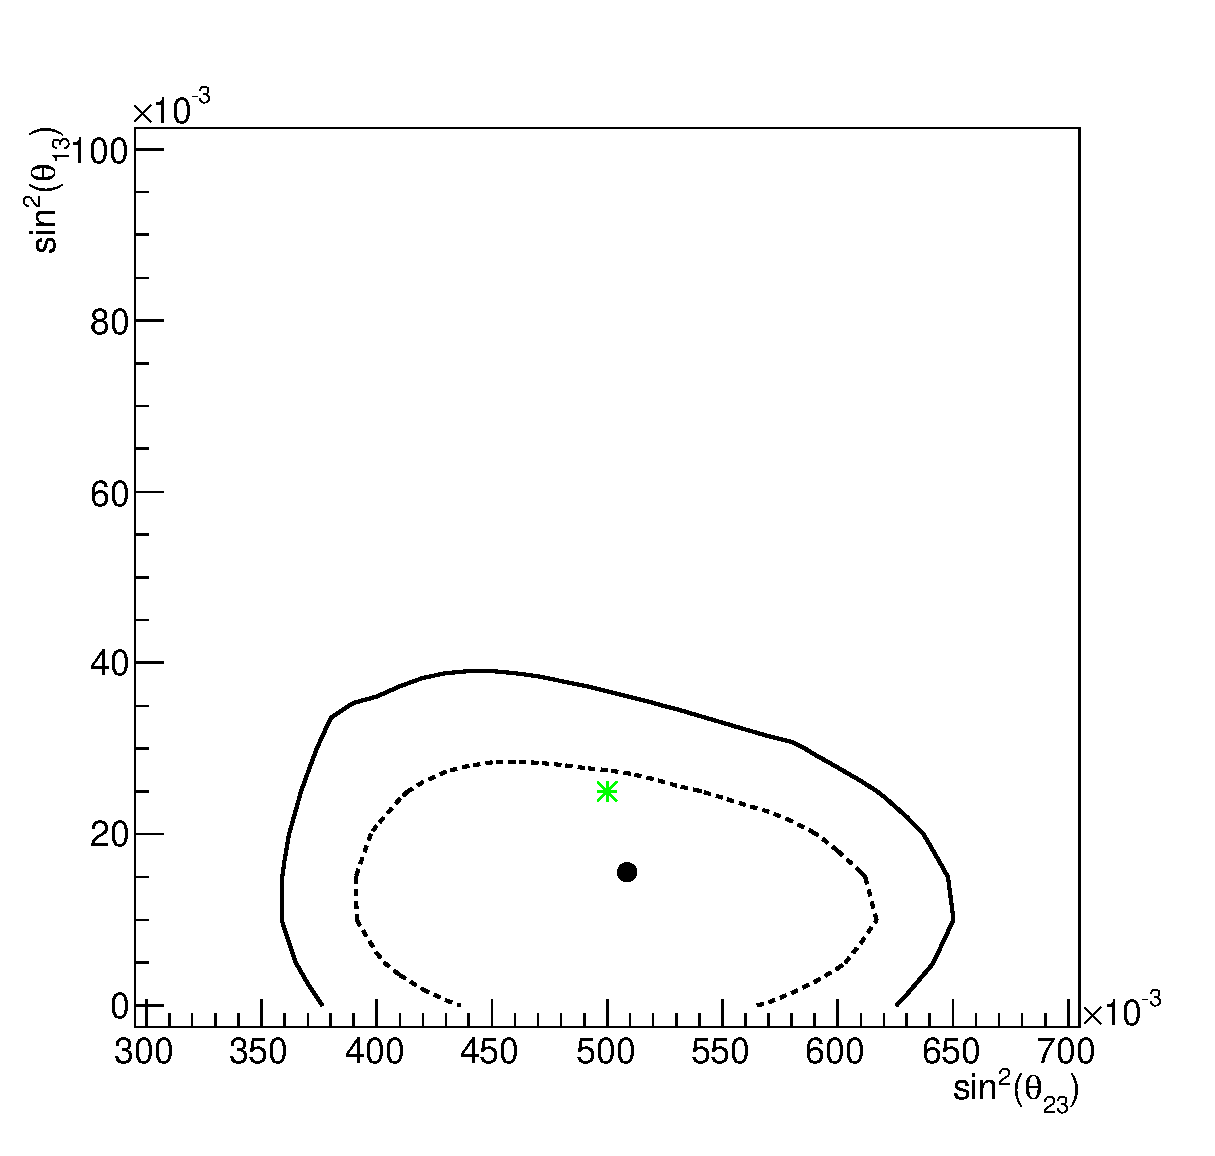
\includegraphics[width=15pc]{./images/appendix/fake_dataset_fits/realistic_fake_dataset0_chisq_theta13_theta23_global_min.eps}
\caption {
  68\% and 90\% CL regions in ($sin^{2}\theta_{23}$, $sin^{2}\theta_{13}$) space for fake dataset \#6.
  At each point, $\chi^2$ was minimized with respect to 
  all oscillation parameters not shown (and not considered to be fixed)
  and all relevant nuisance parameters.
}
\label{fig:toymc6_confreg_sinsqtheta23_sinsqtheta13}
\end{minipage}

\end{figure*}




% 
% 
% ..............................................
% Fake dataset #7
% 
%
\clearpage

\begin{figure*}[htb]

\begin{minipage}[t]{0.46\linewidth}
\center
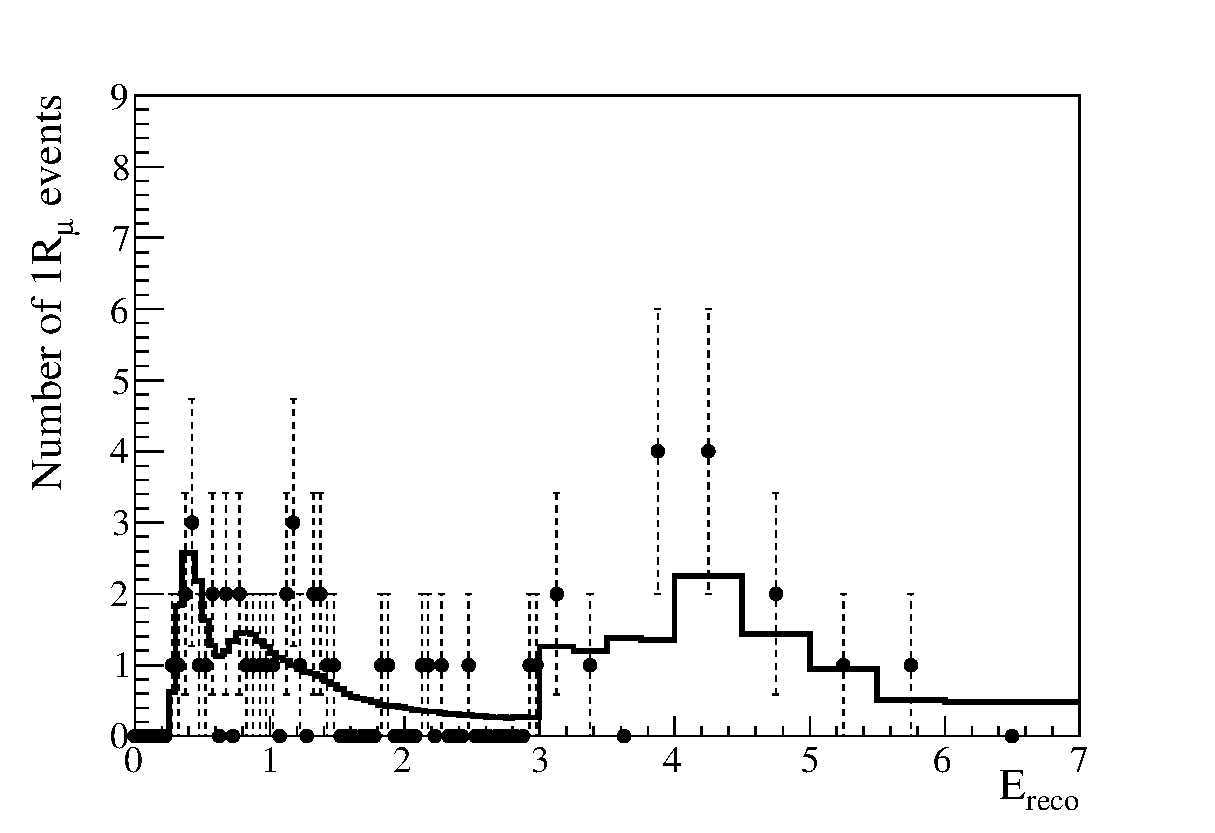
\includegraphics[width=15pc]{./images/appendix/fake_dataset_fits/realistic_fake_dataset1_nh_1st_1Rmu.eps}
\caption {
  Single $\mu$-like ring event best-fit reconstructed energy spectrum
  to fake dataset \#7.
}
\label{fig:toymc7_1Rmu_bestfit_spectrum}
\end{minipage}
\hspace{0.03\linewidth}
\begin{minipage}[t]{0.46\linewidth}
\center
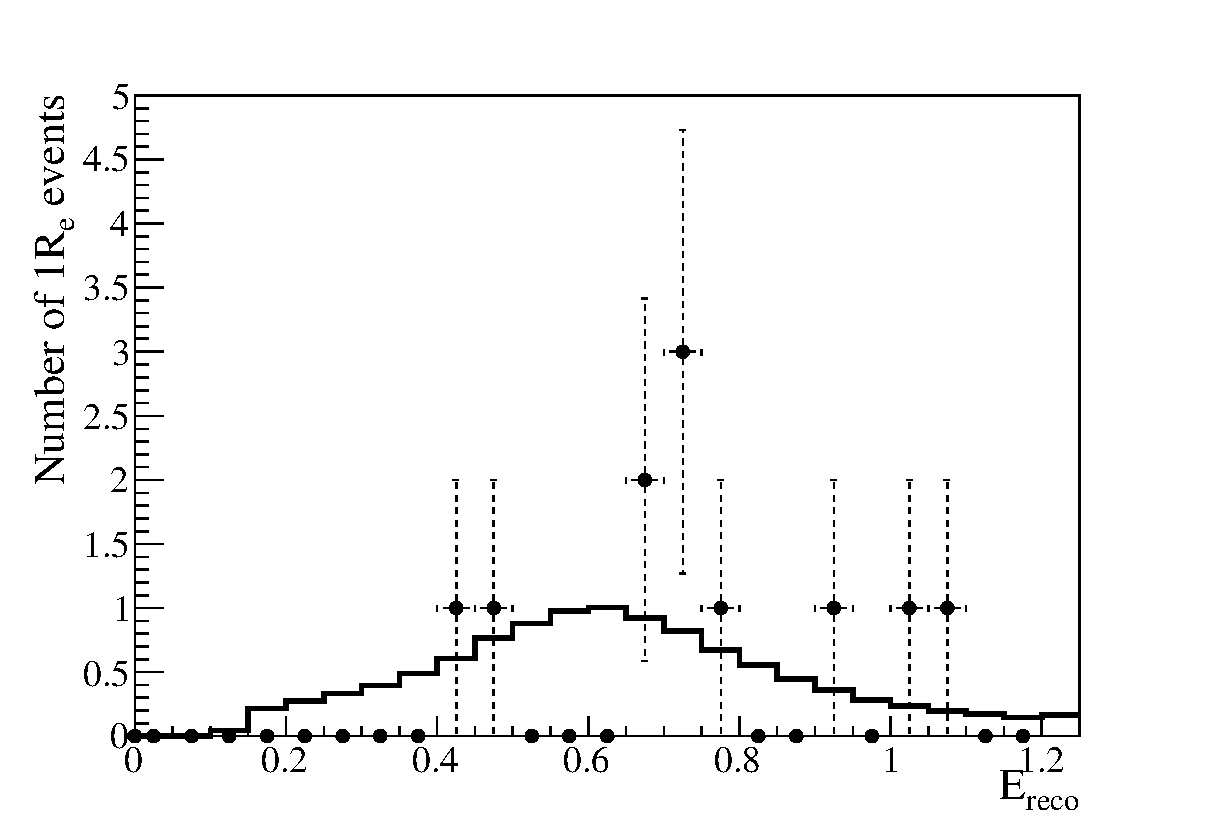
\includegraphics[width=15pc]{./images/appendix/fake_dataset_fits/realistic_fake_dataset1_nh_1st_1Re.eps}
\caption {
  Single e-like ring event best-fit reconstructed energy spectrum
  to fake dataset \#7.
}
\label{fig:toymc7_1Re_bestfit_spectrum}
\end{minipage}

\vfill
\vspace*{0.7cm}

\begin{minipage}[t]{0.90\linewidth}
\center
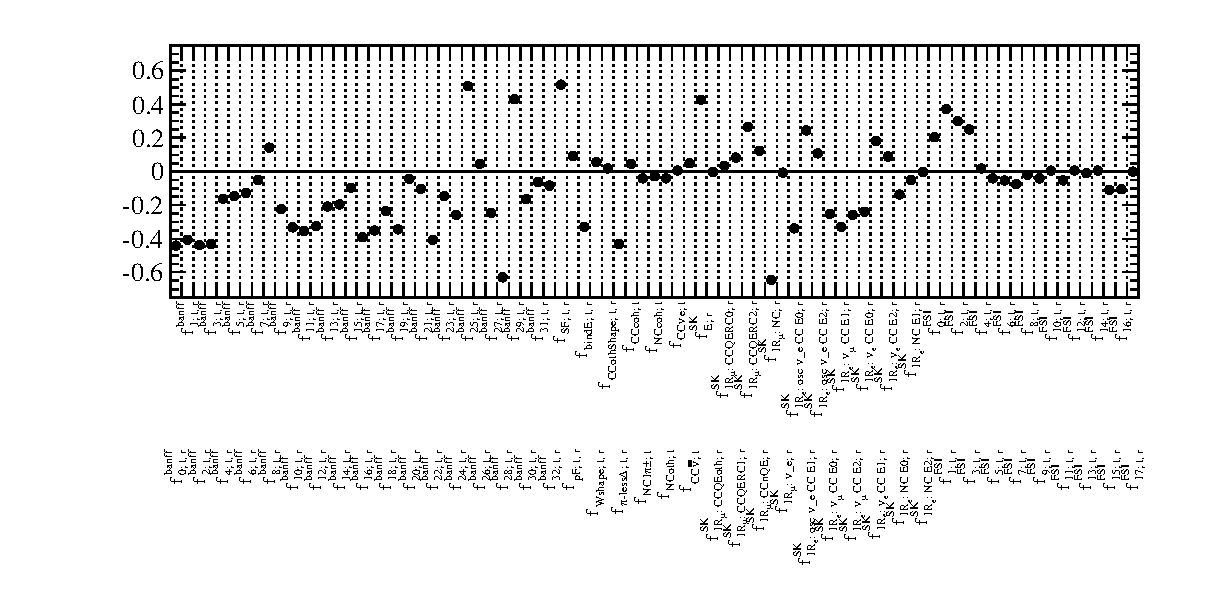
\includegraphics[width=30pc,angle=270]{./images/appendix/fake_dataset_fits/pulls_realistic_fake_dataset1_nh_1st.eps}
\caption {
  Systematic parameter pulls for the oscillation fit to fake dataset \#7.
}
\label{fig:toymc7_pulls}
\end{minipage}

\end{figure*}



%...........................................................
%
% chisq distributions used for calculating the fit p-values
%

\begin{figure*}[htb]

\begin{minipage}[t]{0.90\linewidth}
\center
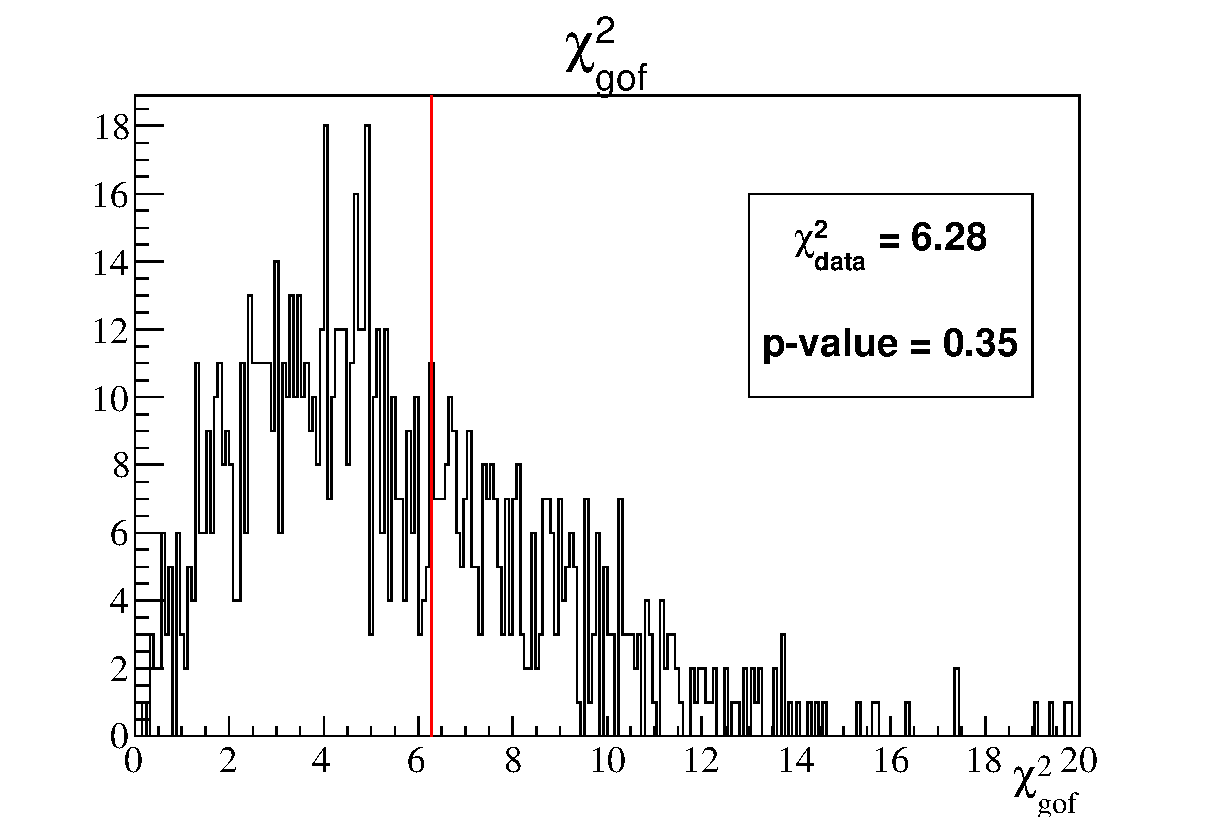
\includegraphics[width=30pc]{./images/appendix/fake_dataset_fits/realistic_fake_dataset1_nh_1st_gof_new.eps}
\caption {
  Distribution of $\chi^2_{gof}$, the goodness-of-fit (gof) $\chi^2$, 
  from 1k toy MC experiments generated at dataset \#7 joint 3-flavour analysis best-fit oscillation point.
  The $\chi^2_{gof}$ value for the dataset \#7 ($\chi^2_{data}$) is highlighted.
  All $\chi^2_{gof}$ values were computed 
  using the 5 (single $\mu$-like ring) + 3 (single e-like ring) 
  reconstructed energy binning scheme described in Sec.\ \ref{sec:goodness_of_fit}.
}
\label{fig:toymc7_gofchisq}
\end{minipage}

\vfill
\vspace*{0.7cm}

\begin{minipage}[t]{0.46\linewidth}
\center
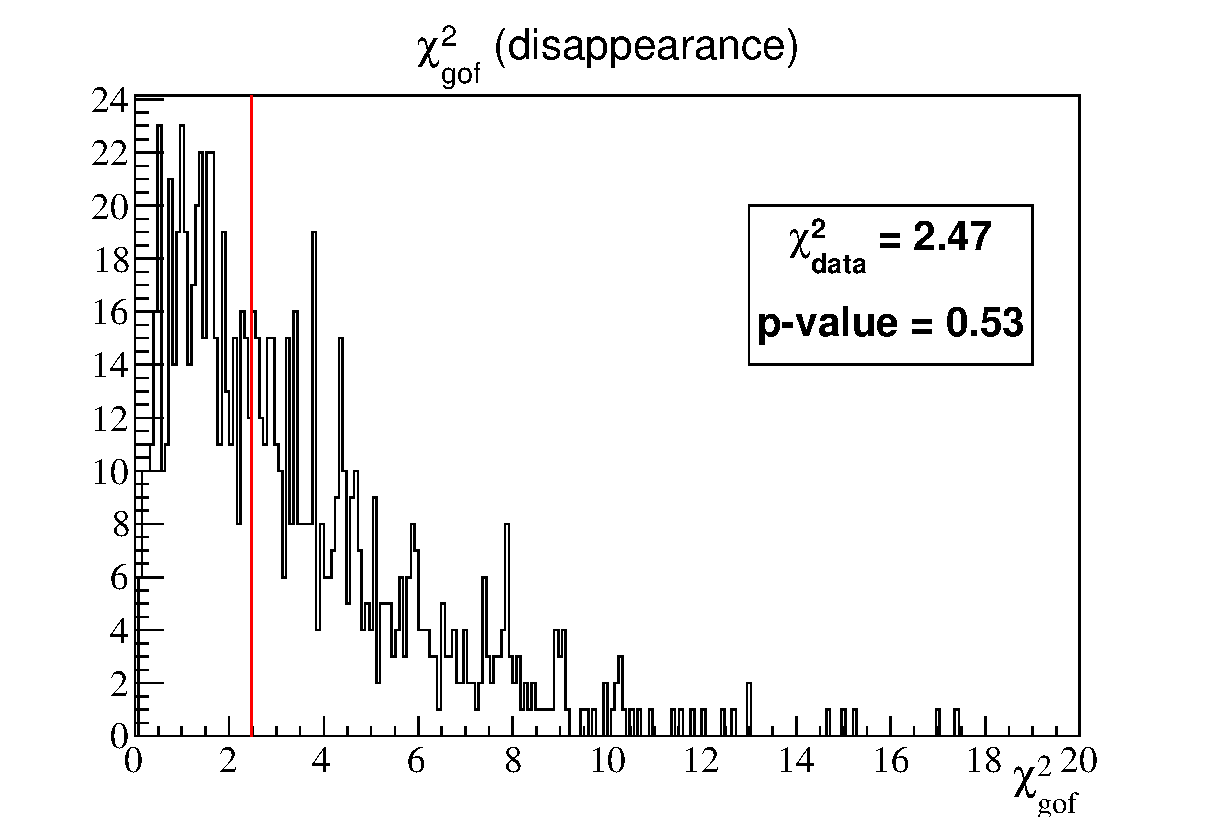
\includegraphics[width=18pc]{./images/appendix/fake_dataset_fits/realistic_fake_dataset1_nh_1st_gof_disap_new.eps}
\caption {
  Distribution of $\chi^2_{gof}$
  from 1k toy MC experiments generated at the dataset \#7 stand-alone 3-flavour $\nu_{\mu}$ disappearance analysis best-fit oscillation point.
  The $\chi^2_{gof}$ value for the dataset \#7 ($\chi^2_{data}$) is highlighted.
  All $\chi^2_{gof}$ values were computed 
  using the 5 (single $\mu$-like ring) 
  reconstructed energy binning scheme described in Sec.\ \ref{sec:goodness_of_fit}.
}
\label{fig:toymc7_gofchisq_disapp}
\end{minipage}
\hspace{0.03\linewidth}
\begin{minipage}[t]{0.46\linewidth}
\center
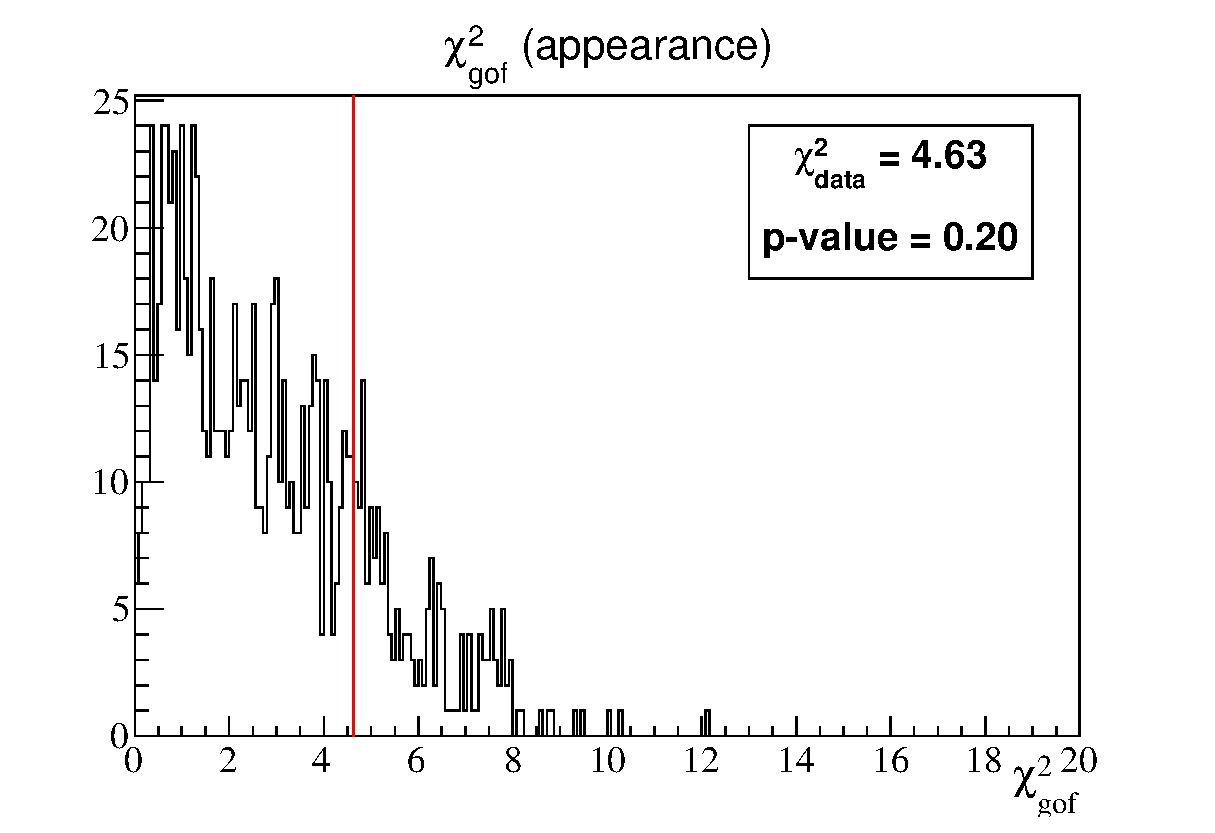
\includegraphics[width=18pc]{./images/appendix/fake_dataset_fits/realistic_fake_dataset1_nh_1st_gof_app_new.eps}
\caption {
  Distribution of $\chi^2_{gof}$
  from 1k toy MC experiments generated at the dataset \#7 stand-alone 3-flavour $\nu_{e}$ appearance analysis best-fit oscillation point.
  The $\chi^2_{gof}$ value for the dataset \#7 ($\chi^2_{data}$) is highlighted.
  All $\chi^2_{gof}$ values were computed 
  using the 3 (single e-like ring) 
  reconstructed energy binning scheme  as described in Sec.\ \ref{sec:goodness_of_fit}.
}
\label{fig:toymc7_gofchisq_app}
\end{minipage}

\end{figure*}



%
% delta\chisq and contours
%

\begin{figure*}[htb]

\begin{minipage}[t]{0.22\linewidth}
\center
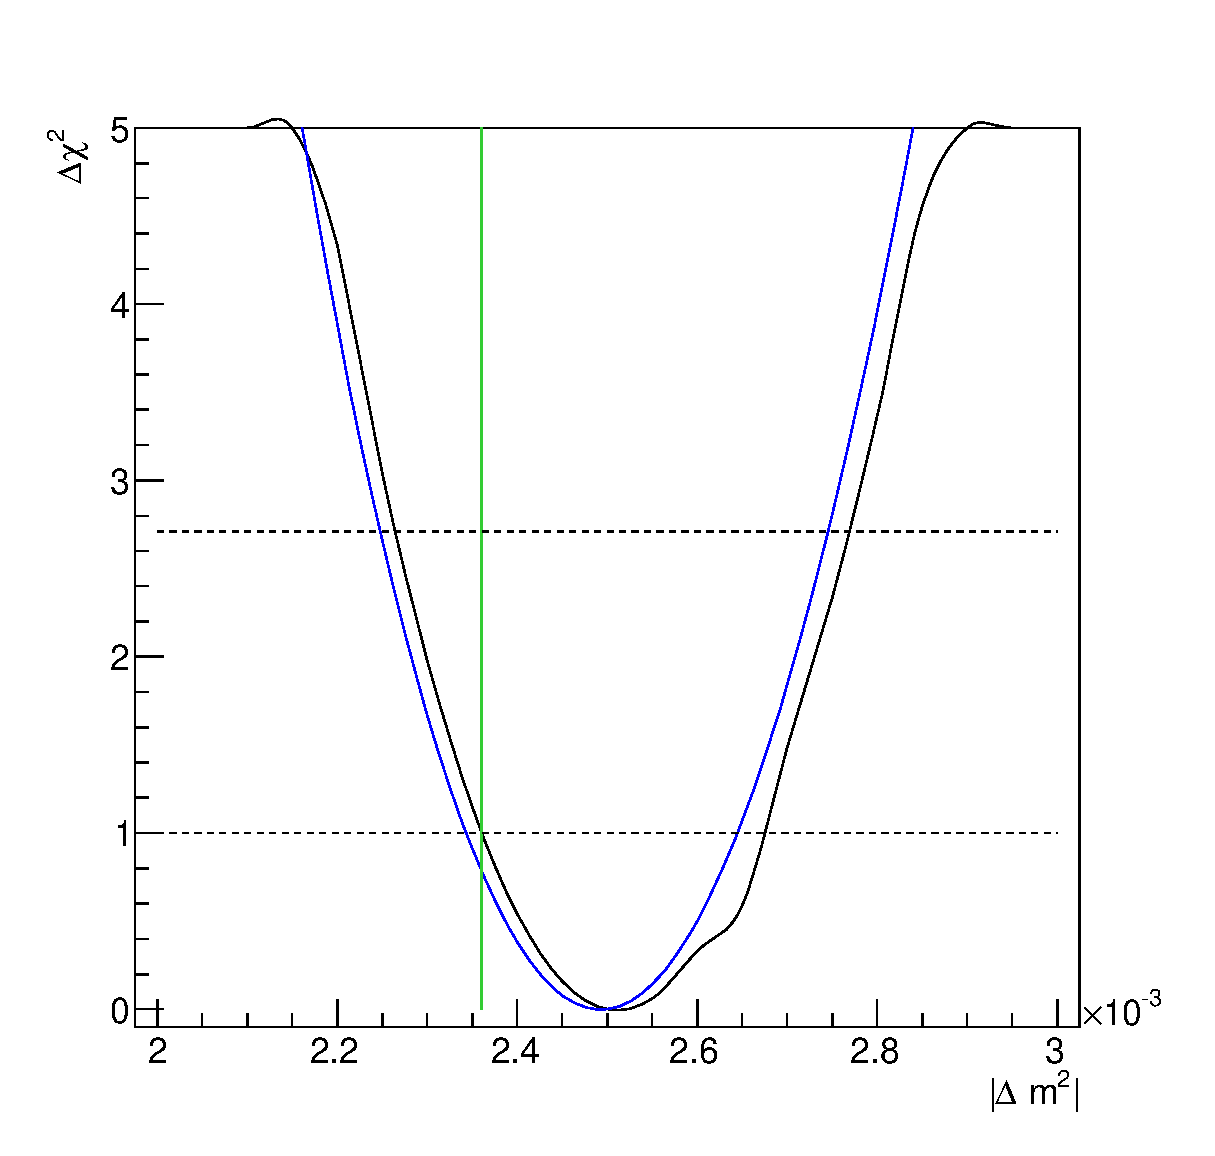
\includegraphics[width=9pc]{./images/appendix/fake_dataset_fits/realistic_fake_dataset1_chisq_dm23sq_global_min.eps}
\caption {
  $\Delta\chi^2$ as function of $|\Delta m^{2}|$ for fake dataset \#7.
  At each point, $\chi^2$ was minimized with respect to 
  $\sin^{2}\theta_{23}$, $\sin^{2}\theta_{13}$, $\delta_{CP}$
  and all relevant nuisance parameters for the joint analysis (black)
  and with respect to $\sin^{2}\theta_{23}$ and all relevant nuisance
  parameters for the disappearance analysis (blue).
}
\label{fig:toymc7_dchisq_Dmsq}
\end{minipage}
\hspace{0.02\linewidth}
\begin{minipage}[t]{0.22\linewidth}
\center
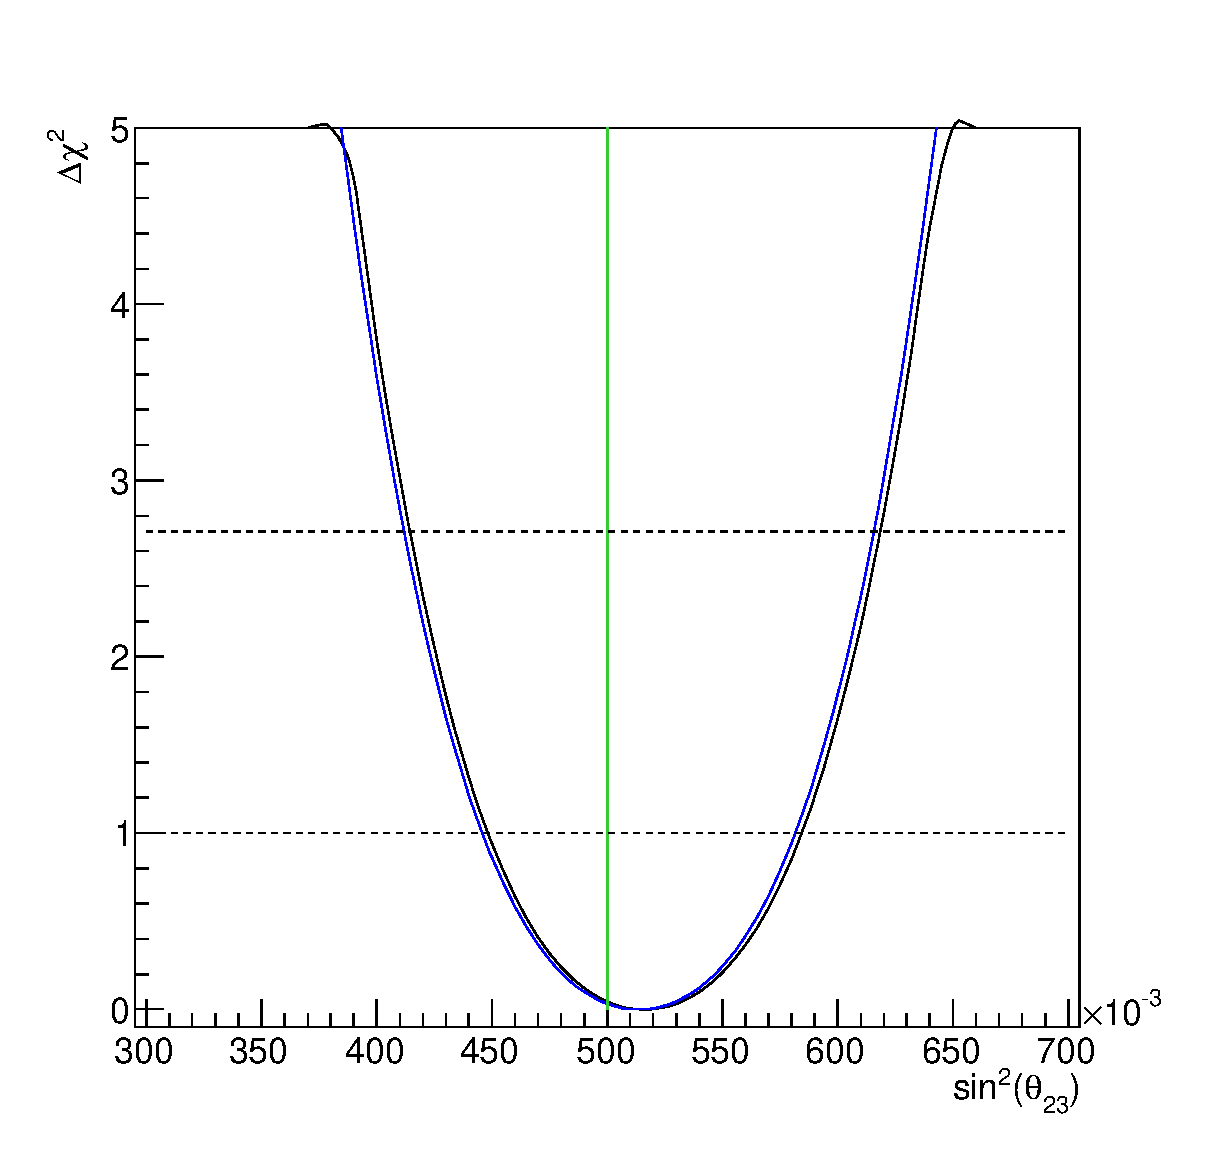
\includegraphics[width=9pc]{./images/appendix/fake_dataset_fits/realistic_fake_dataset1_chisq_theta23_global_min.eps}
\caption {
  $\Delta\chi^2$ as function of $sin^{2}\theta_{23}$ for fake dataset \#7.
  At each point, $\chi^2$ was minimized with respect to 
  $|\Delta m^{2}|$, $\sin^{2}\theta_{13}$, $\delta_{CP}$
  and all relevant nuisance parameters for the joint analysis (black)
  and with respect to $\sin^{2}\theta_{23}$ and all relevant nuisance
  parameters for the disappearance analysis (blue).
}
\label{fig:toymc7_dchisq_sinsqtheta23}
\end{minipage}
\hspace{0.02\linewidth}
\begin{minipage}[t]{0.22\linewidth}
\center
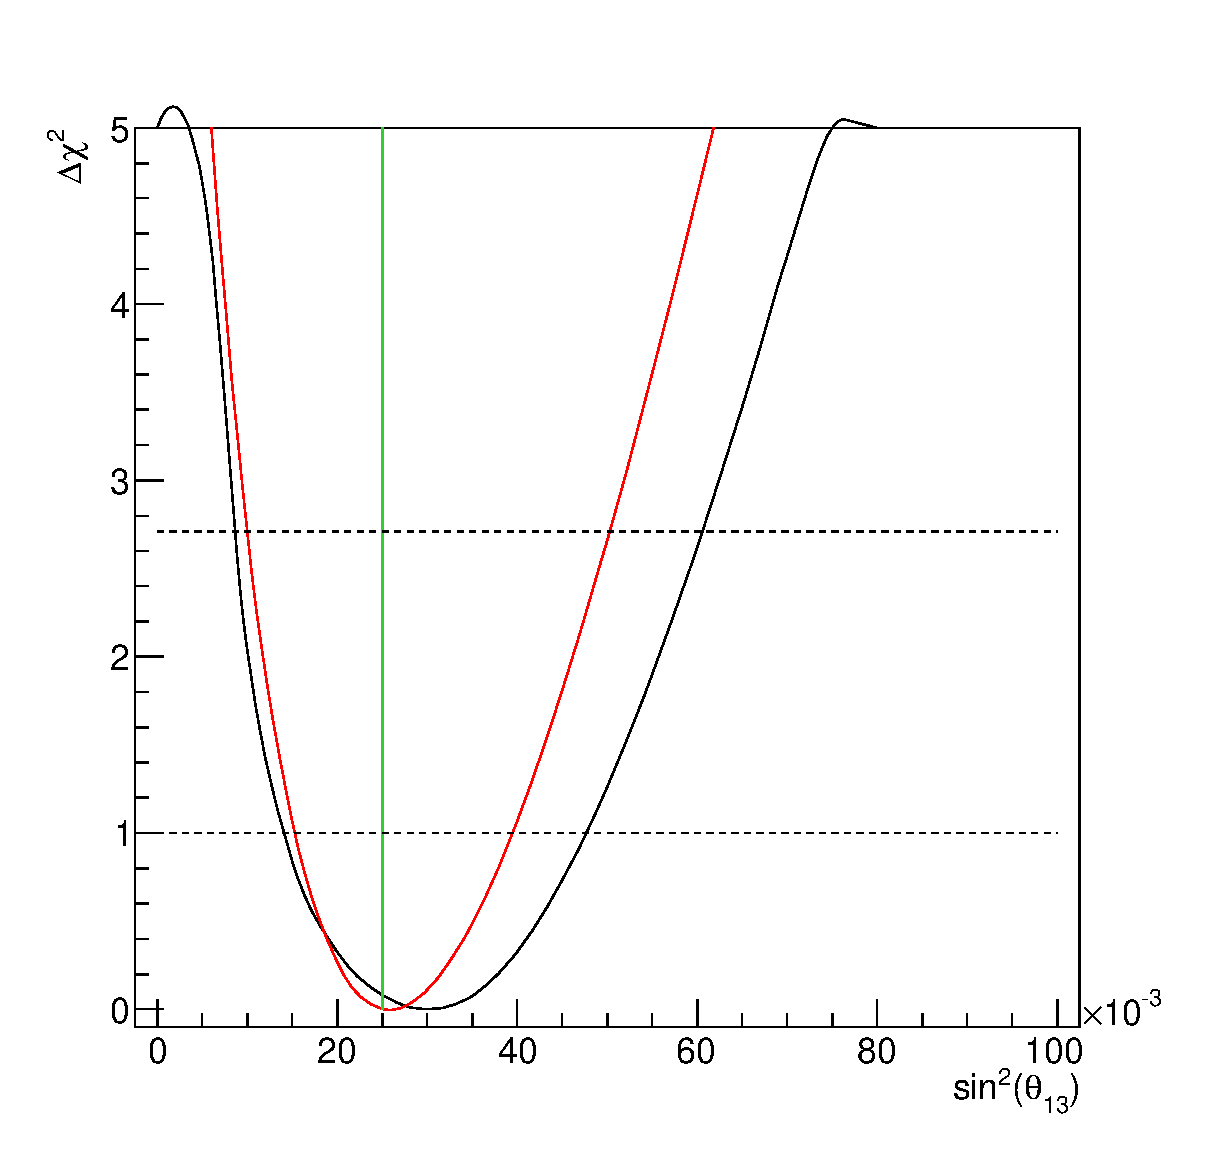
\includegraphics[width=9pc]{./images/appendix/fake_dataset_fits/realistic_fake_dataset1_chisq_theta13_global_min.eps}
\caption {
  $\Delta\chi^2$ as function of $sin^{2}\theta_{13}$ for fake dataset \#7.
  At each point, $\chi^2$ was minimized with respect to 
  $\sin^{2}\theta_{23}$, $\sin^{2}\theta_{13}$, $\delta_{CP}$
  and all relevant nuisance parameters for the joint analysis (black)
  and with respect to all relevant nuisance parameters 
  ($\delta_{CP}$ is fixed to 0) for the appearance analysis (red).
}
\label{fig:toymc7_dchisq_sinsqtheta13}
\end{minipage}
\hspace{0.02\linewidth}
\begin{minipage}[t]{0.22\linewidth}
\center
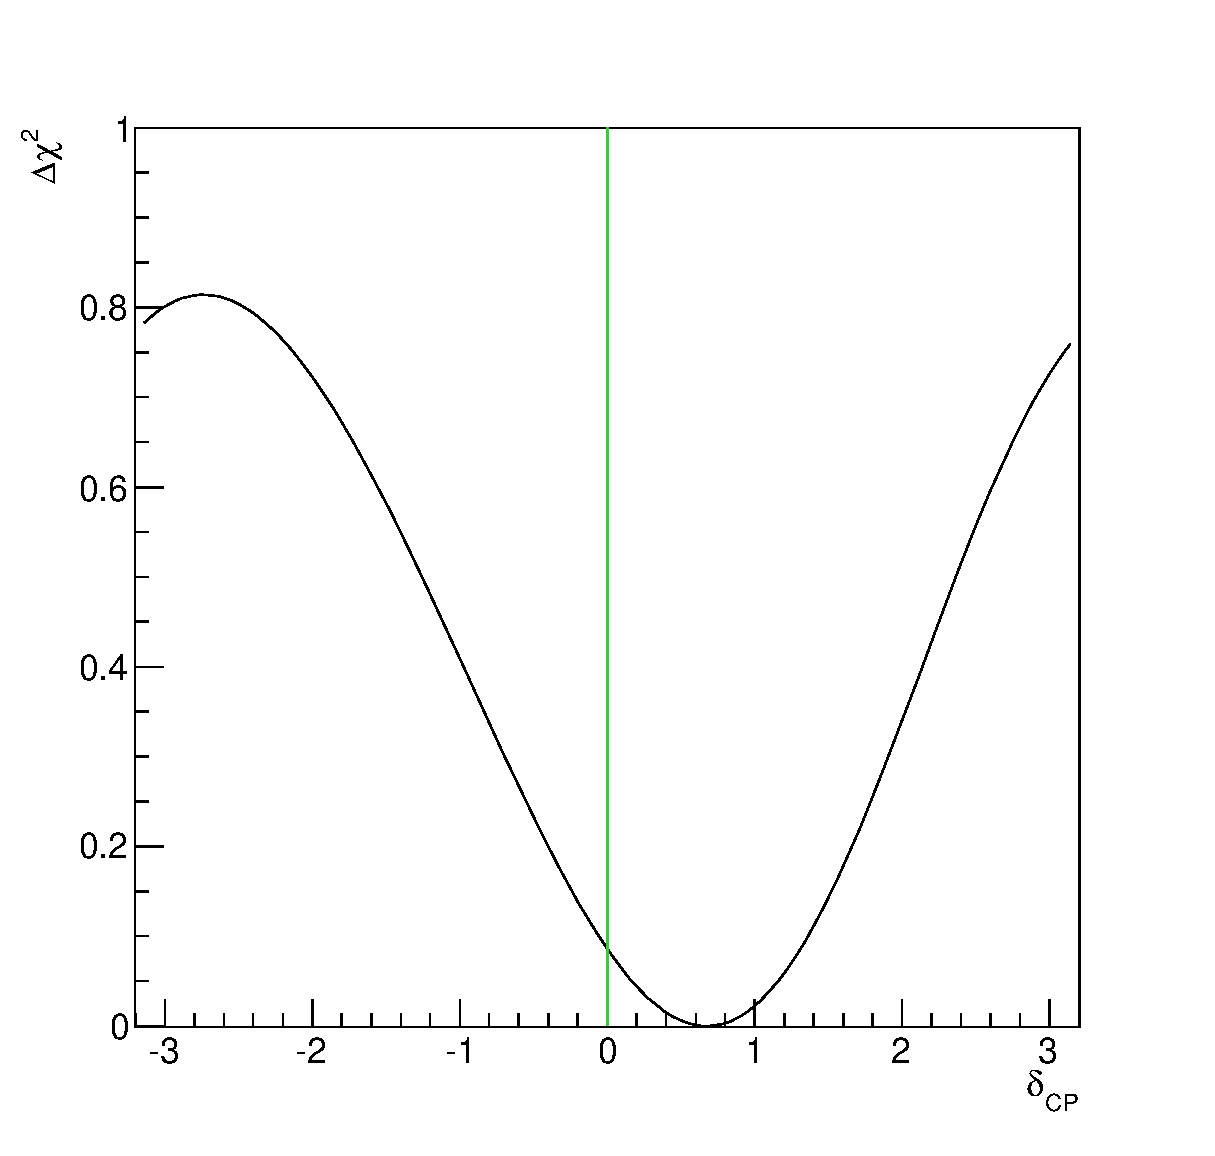
\includegraphics[width=9pc]{.//images/appendix/fake_dataset_fits/realistic_fake_dataset1_chisq_deltacp_global_min.eps}
\caption {
  $\Delta\chi^2$ as function of $\delta_{CP}$ for fake dataset \#7.
  At each point, $\chi^2$ was minimized with respect to 
  all oscillation parameters not shown (and not considered to be fixed)
  and all relevant nuisance parameters.
}
\label{fig:toymc7_dchisq_deltacp}
\end{minipage}
\vfill
\vspace*{0.7cm}
\begin{minipage}[t]{0.48\linewidth}
\center
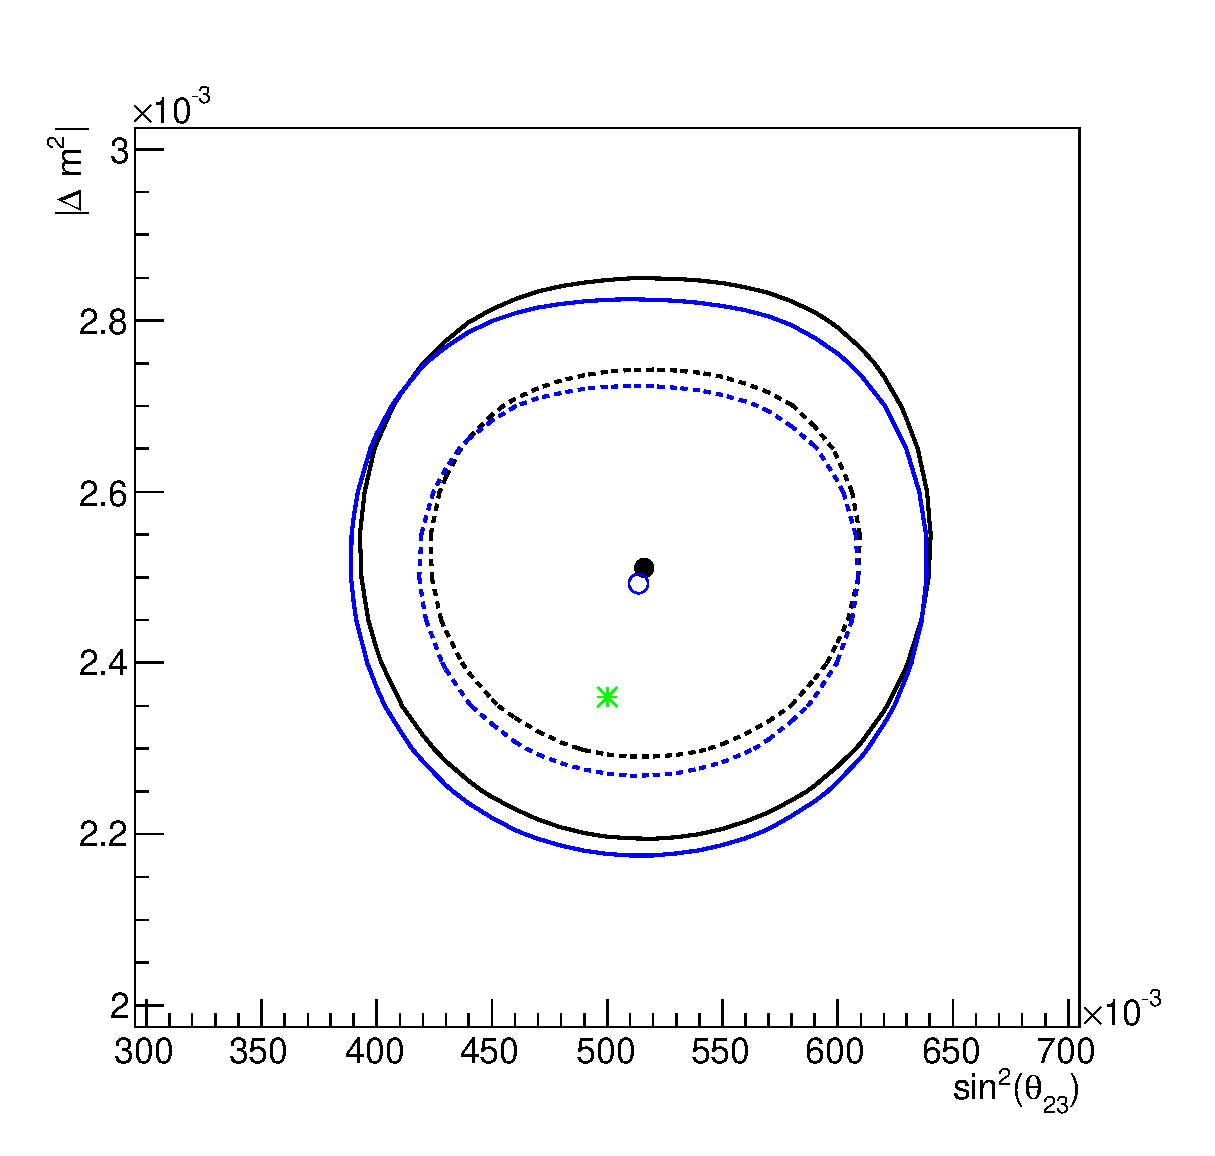
\includegraphics[width=15pc]{./images/appendix/fake_dataset_fits/realistic_fake_dataset1_chisq_theta23_dm23sq_global_min.eps}
\caption {
  68\% and 90\% CL regions in ($sin^{2}\theta_{23}$, $|\Delta m^{2}|$) space for fake dataset \#7.
  At each point, $\chi^2$ was minimized with respect to 
  $\sin^{2}\theta_{13}$, $\delta_{CP}$
  and all relevant nuisance parameters for the joint analysis (black)
  and with respect to all relevant nuisance parameters for the disappearance analysis (blue).
}
\label{fig:toymc7_confreg_sinsqtheta23_Dmsq}
\end{minipage}
\hspace{0.03\linewidth}
\begin{minipage}[t]{0.48\linewidth}
\center
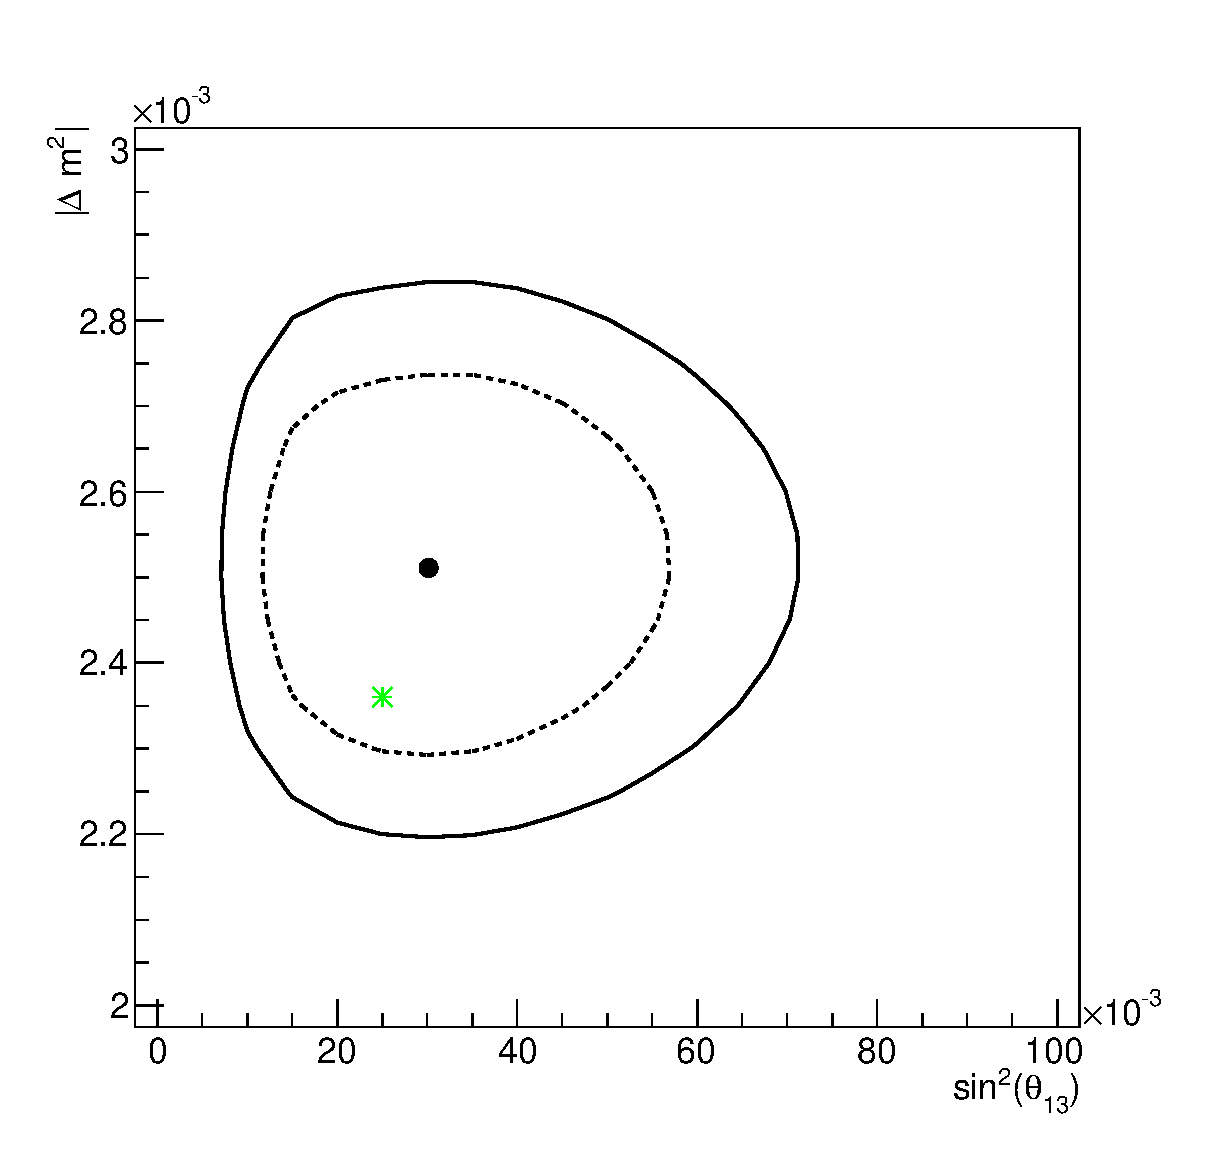
\includegraphics[width=15pc]{./images/appendix/fake_dataset_fits/realistic_fake_dataset1_chisq_theta13_dm23sq_global_min.eps}
\caption {
  68\% and 90\% CL regions in ($sin^{2}\theta_{13}$, $|\Delta m^{2}|$) space for fake dataset \#7.
  At each point, $\chi^2$ was minimized with respect to 
  all oscillation parameters not shown (and not considered to be fixed)
  and all relevant nuisance parameters.
}
\label{fig:toymc7_confreg_sinsqtheta13_Dmsq}
\end{minipage}

\vfill
\vspace*{0.7cm}

\begin{minipage}[t]{0.48\linewidth}
\center
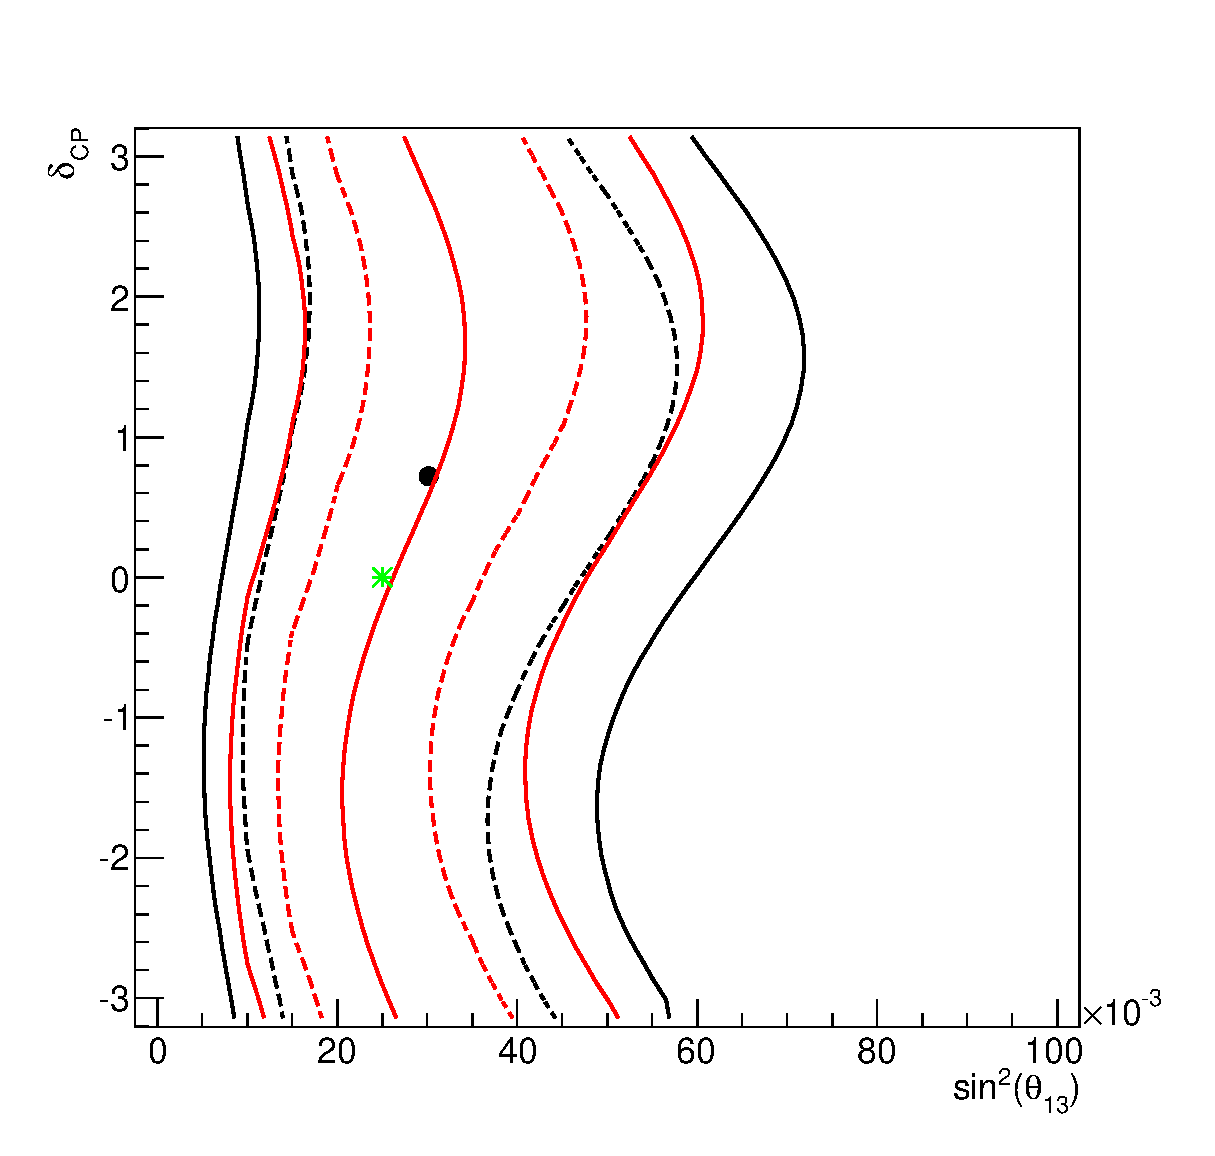
\includegraphics[width=15pc]{./images/appendix/fake_dataset_fits/realistic_fake_dataset1_chisq_theta13_deltacp_global_min.eps}
\caption {
  68\% and 90\% CL regions in ($sin^{2}\theta_{13}$, $\delta_{CP}$) space for fake dataset \#7.
  At each point, $\chi^2$ was minimized with respect to 
  $|\Delta m^{2}|$, $\sin^{2}\theta_{23}$
  and all relevant nuisance parameters for the joint analysis (black)
  and with respect to all relevant nuisance parameters for the appearance analysis (red).
  Notice that different methods are used to
  construct confidence regions for the joint analysis (global minimum) and for the 
  stand-alone appearance analysis (raster scan).
}
\label{fig:toymc7_confreg_sinsqtheta13_deltacp}
\end{minipage}
\hspace{0.03\linewidth}
\begin{minipage}[t]{0.48\linewidth}
\center
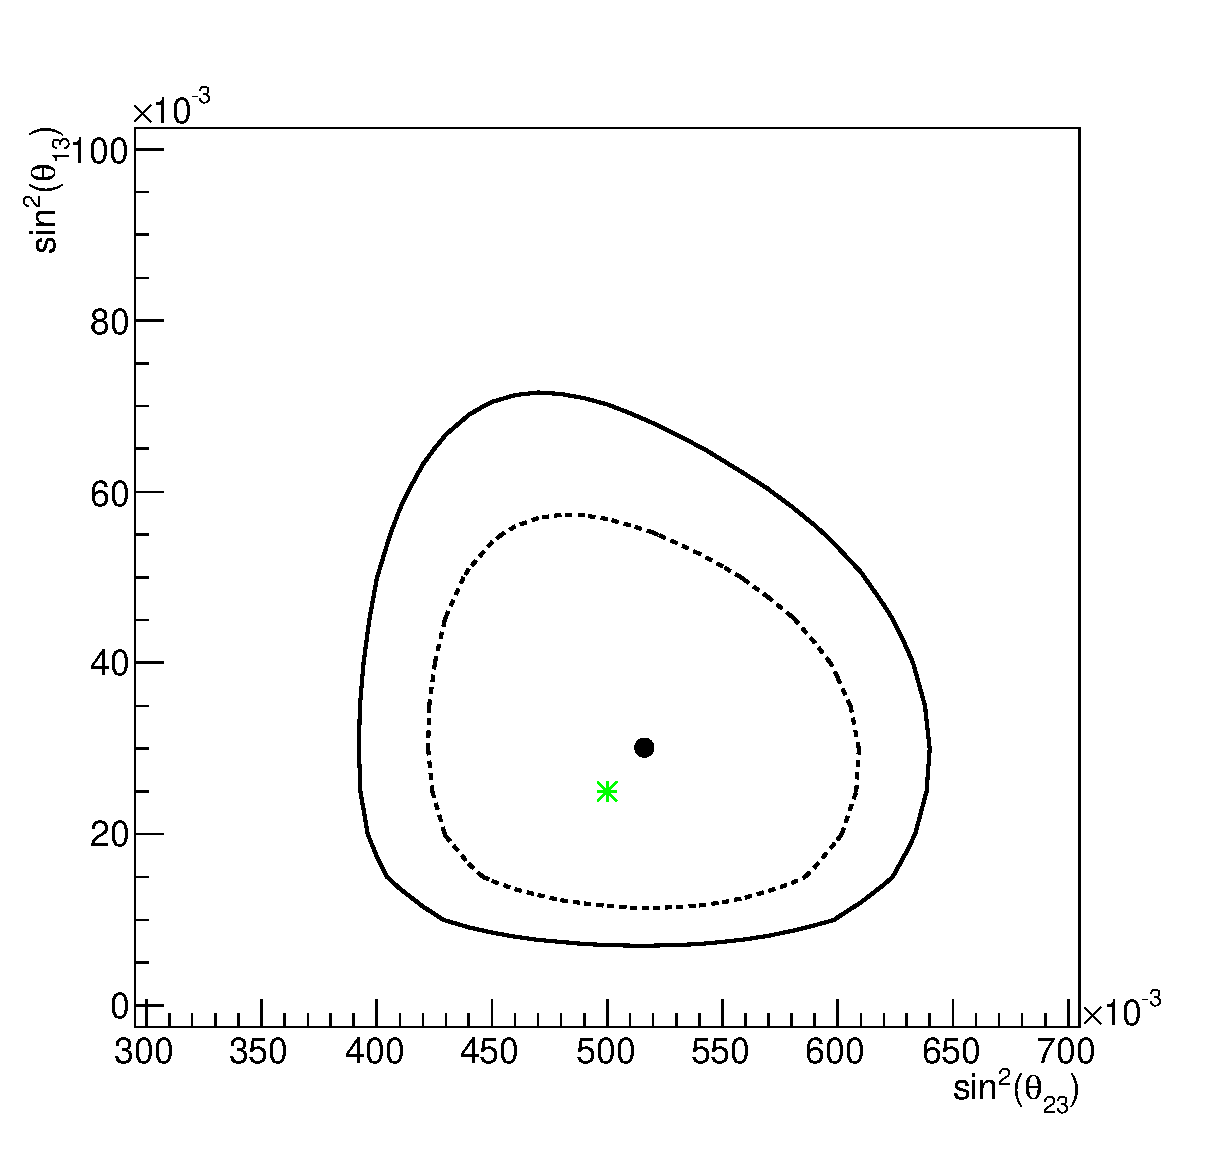
\includegraphics[width=15pc]{./images/appendix/fake_dataset_fits/realistic_fake_dataset1_chisq_theta13_theta23_global_min.eps}
\caption {
  68\% and 90\% CL regions in ($sin^{2}\theta_{23}$, $sin^{2}\theta_{13}$) space for fake dataset \#7.
  At each point, $\chi^2$ was minimized with respect to 
  all oscillation parameters not shown (and not considered to be fixed)
  and all relevant nuisance parameters.
}
\label{fig:toymc7_confreg_sinsqtheta23_sinsqtheta13}
\end{minipage}

\end{figure*}



% 
% 
% ..............................................
% Fake dataset #8
% 
%
\clearpage

\begin{figure*}[htb]

\begin{minipage}[t]{0.46\linewidth}
\center
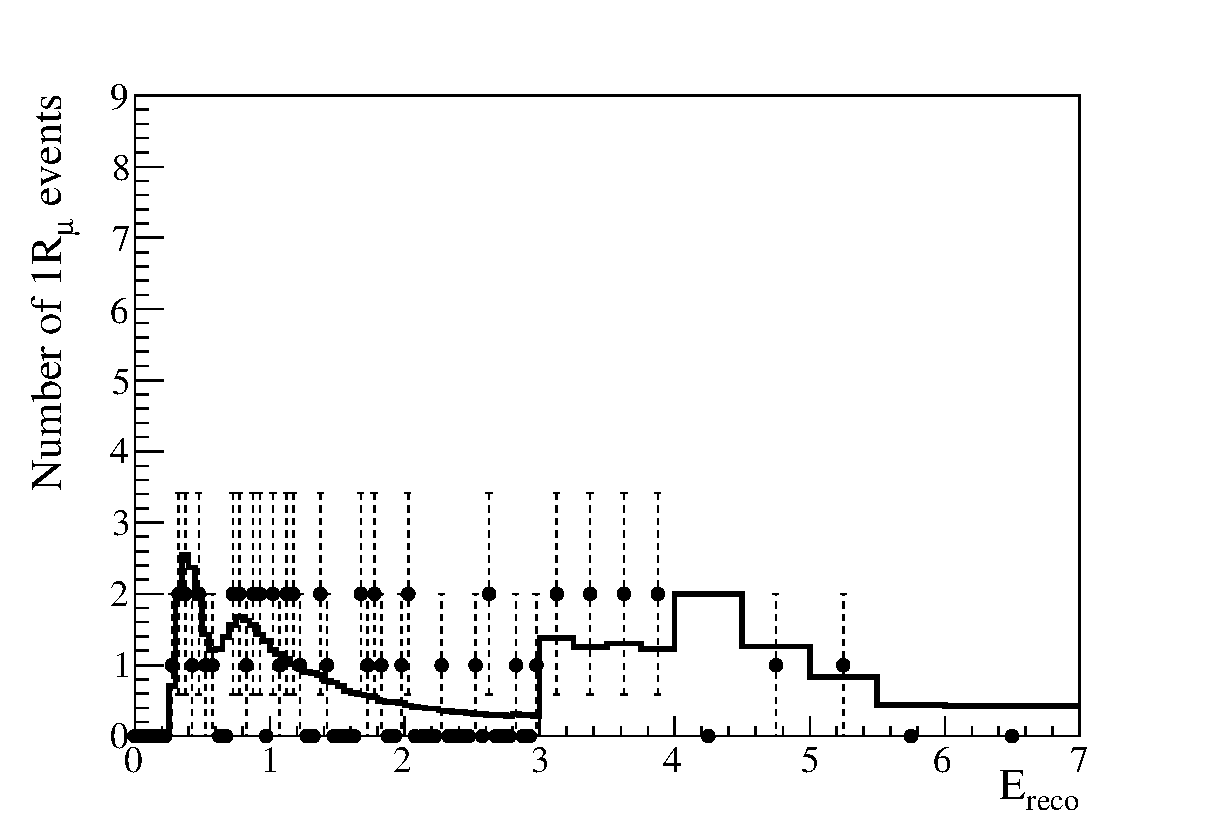
\includegraphics[width=15pc]{./images/appendix/fake_dataset_fits/realistic_fake_dataset7_nh_1st_1Rmu.eps}
\caption {
  Single $\mu$-like ring event best-fit reconstructed energy spectrum
  to fake dataset \#8.
}
\label{fig:toymc8_1Rmu_bestfit_spectrum}
\end{minipage}
\hspace{0.03\linewidth}
\begin{minipage}[t]{0.46\linewidth}
\center
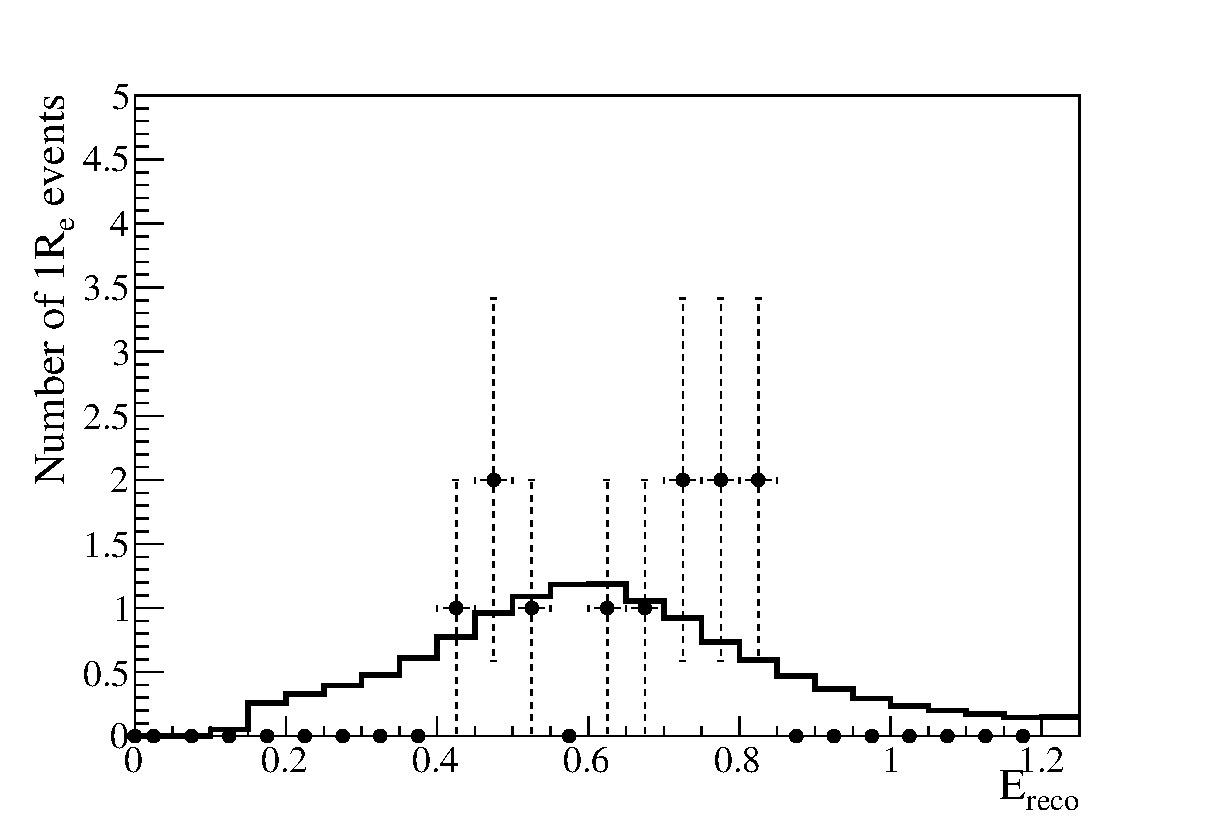
\includegraphics[width=15pc]{./images/appendix/fake_dataset_fits/realistic_fake_dataset7_nh_1st_1Re.eps}
\caption {
  Single e-like ring event best-fit reconstructed energy spectrum
  to fake dataset \#8.
}
\label{fig:toymc8_1Re_bestfit_spectrum}
\end{minipage}

\vfill
\vspace*{0.7cm}

\begin{minipage}[t]{0.90\linewidth}
\center
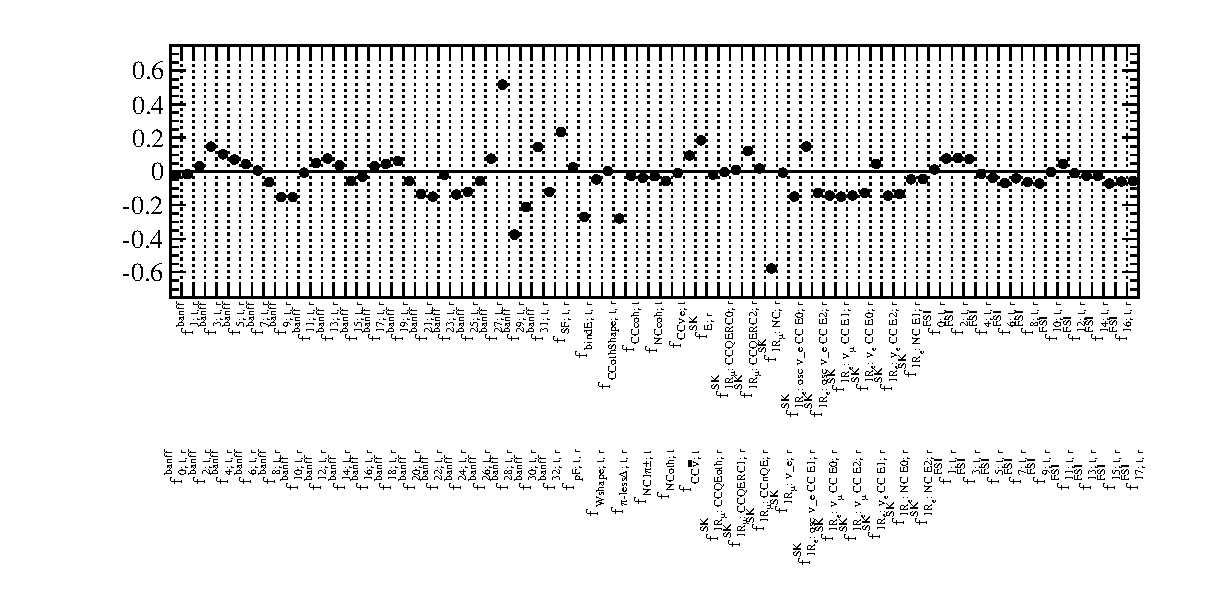
\includegraphics[width=30pc,angle=270]{./images/appendix/fake_dataset_fits/pulls_realistic_fake_dataset7_nh_1st.eps}
\caption {
  Systematic parameter pulls for the oscillation fit to fake dataset \#8.
}
\label{fig:toymc8_pulls}
\end{minipage}

\end{figure*}


%...........................................................
%
% chisq distributions used for calculating the fit p-values
%

\begin{figure*}[htb]

\begin{minipage}[t]{0.90\linewidth}
\center
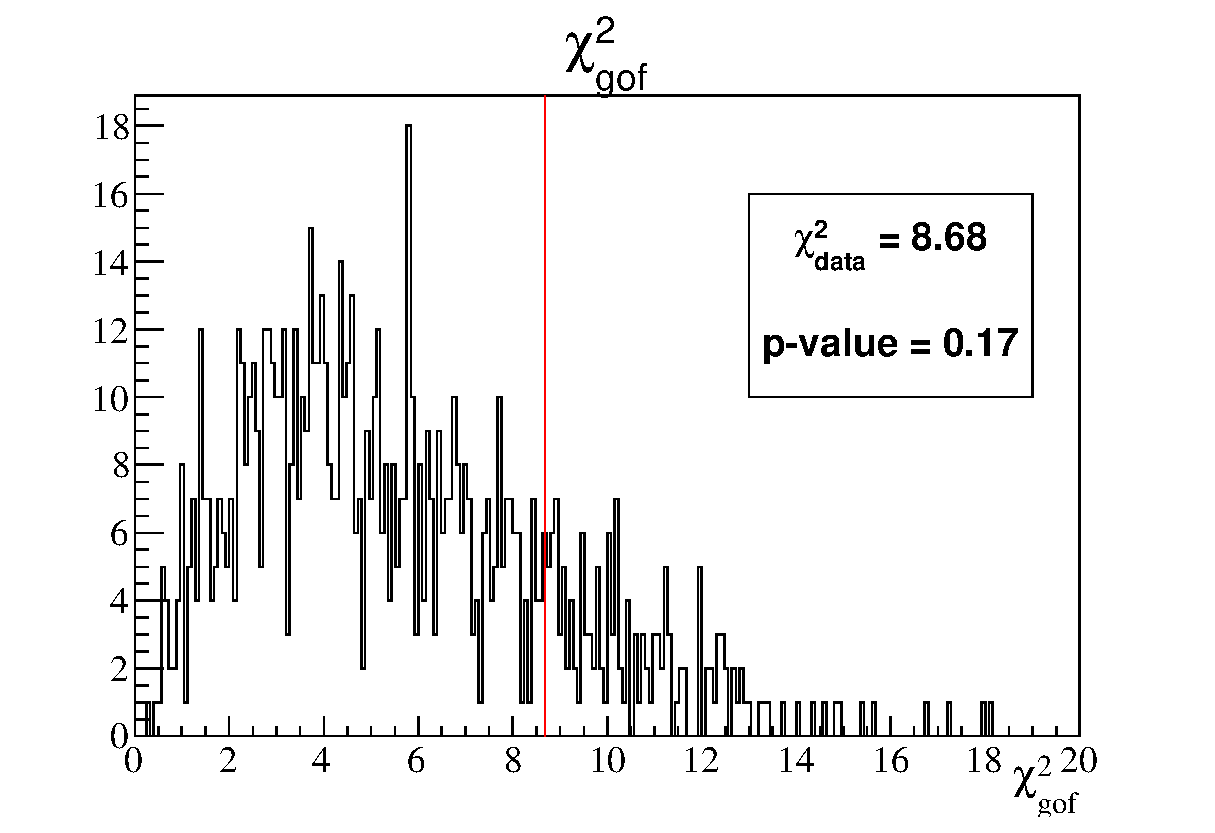
\includegraphics[width=30pc]{./images/appendix/fake_dataset_fits/realistic_fake_dataset7_nh_1st_gof_new.eps}
\caption {
  Distribution of $\chi^2_{gof}$, the goodness-of-fit (gof) $\chi^2$, 
  from 1k toy MC experiments generated at dataset \#8 joint 3-flavour analysis best-fit oscillation point.
  The $\chi^2_{gof}$ value for the dataset \#8 ($\chi^2_{data}$) is highlighted.
  All $\chi^2_{gof}$ values were computed 
  using the 5 (single $\mu$-like ring) + 3 (single e-like ring) 
  reconstructed energy binning scheme described in Sec.\ \ref{sec:goodness_of_fit}.
}
\label{fig:toymc8_gofchisq}
\end{minipage}

\vfill
\vspace*{0.7cm}

\begin{minipage}[t]{0.46\linewidth}
\center
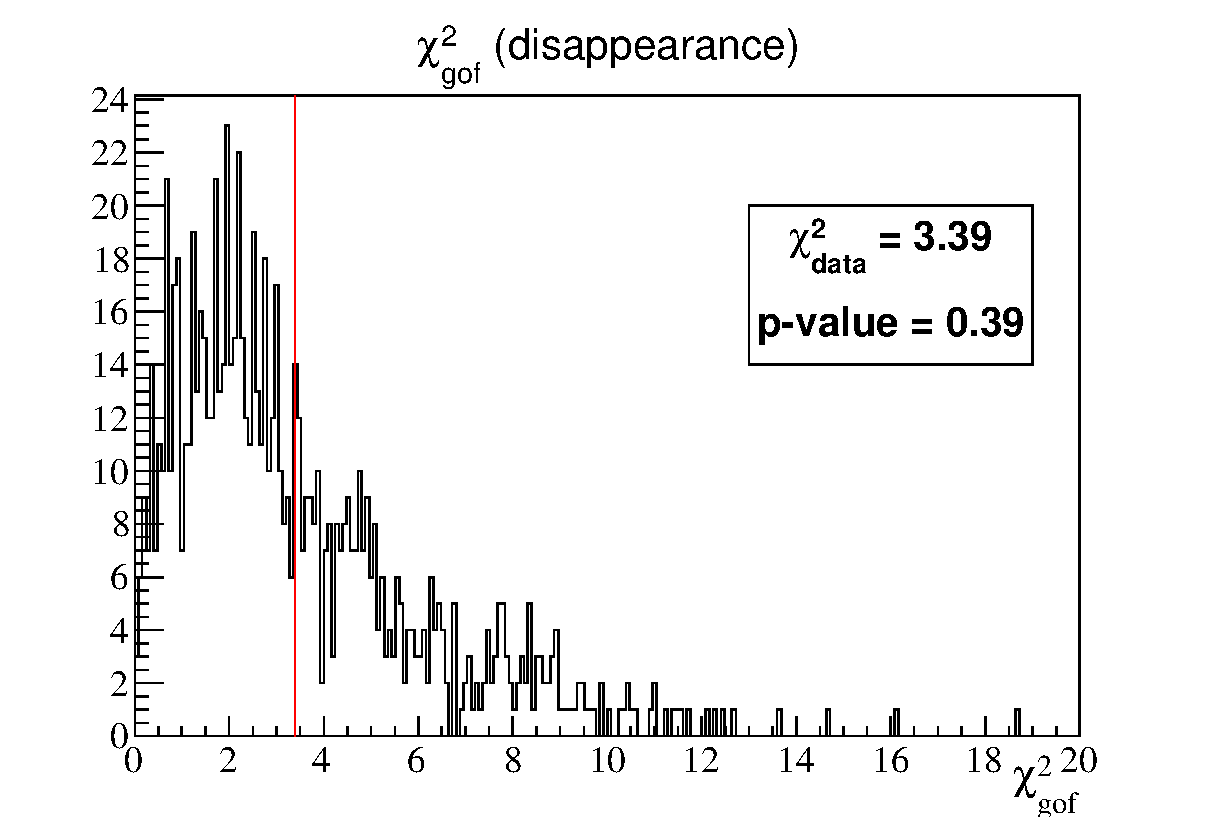
\includegraphics[width=18pc]{./images/appendix/fake_dataset_fits/realistic_fake_dataset7_nh_1st_gof_disap_new.eps}
\caption {
  Distribution of $\chi^2_{gof}$
  from 1k toy MC experiments generated at the dataset \#8 stand-alone 3-flavour $\nu_{\mu}$ disappearance analysis best-fit oscillation point.
  The $\chi^2_{gof}$ value for the dataset \#8 ($\chi^2_{data}$) is highlighted.
  All $\chi^2_{gof}$ values were computed 
  using the 5 (single $\mu$-like ring) 
  reconstructed energy binning scheme described in Sec.\ \ref{sec:goodness_of_fit}.
}
\label{fig:toymc8_gofchisq_disapp}
\end{minipage}
\hspace{0.03\linewidth}
\begin{minipage}[t]{0.46\linewidth}
\center
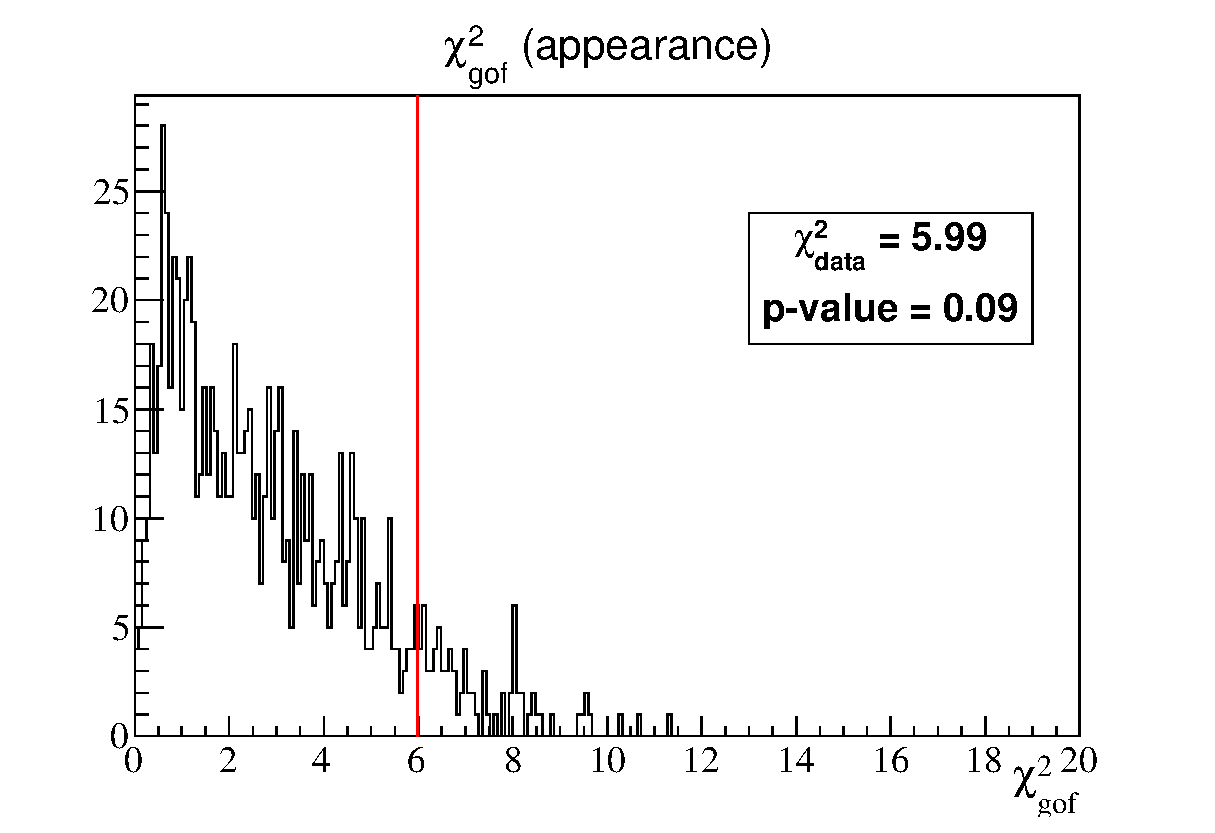
\includegraphics[width=18pc]{./images/appendix/fake_dataset_fits/realistic_fake_dataset7_nh_1st_gof_app_new.eps}
\caption {
  Distribution of $\chi^2_{gof}$
  from 1k toy MC experiments generated at the dataset \#8 stand-alone 3-flavour $\nu_{e}$ appearance analysis best-fit oscillation point.
  The $\chi^2_{gof}$ value for the dataset \#8 ($\chi^2_{data}$) is highlighted.
   All $\chi^2_{gof}$ values were computed 
  using the 3 (single e-like ring) 
  reconstructed energy binning scheme  as described in Sec.\ \ref{sec:goodness_of_fit}.
}
\label{fig:toymc8_gofchisq_app}
\end{minipage}

\end{figure*}



%
% delta\chisq and contours
%

\begin{figure*}[htb]

\begin{minipage}[t]{0.22\linewidth}
\center
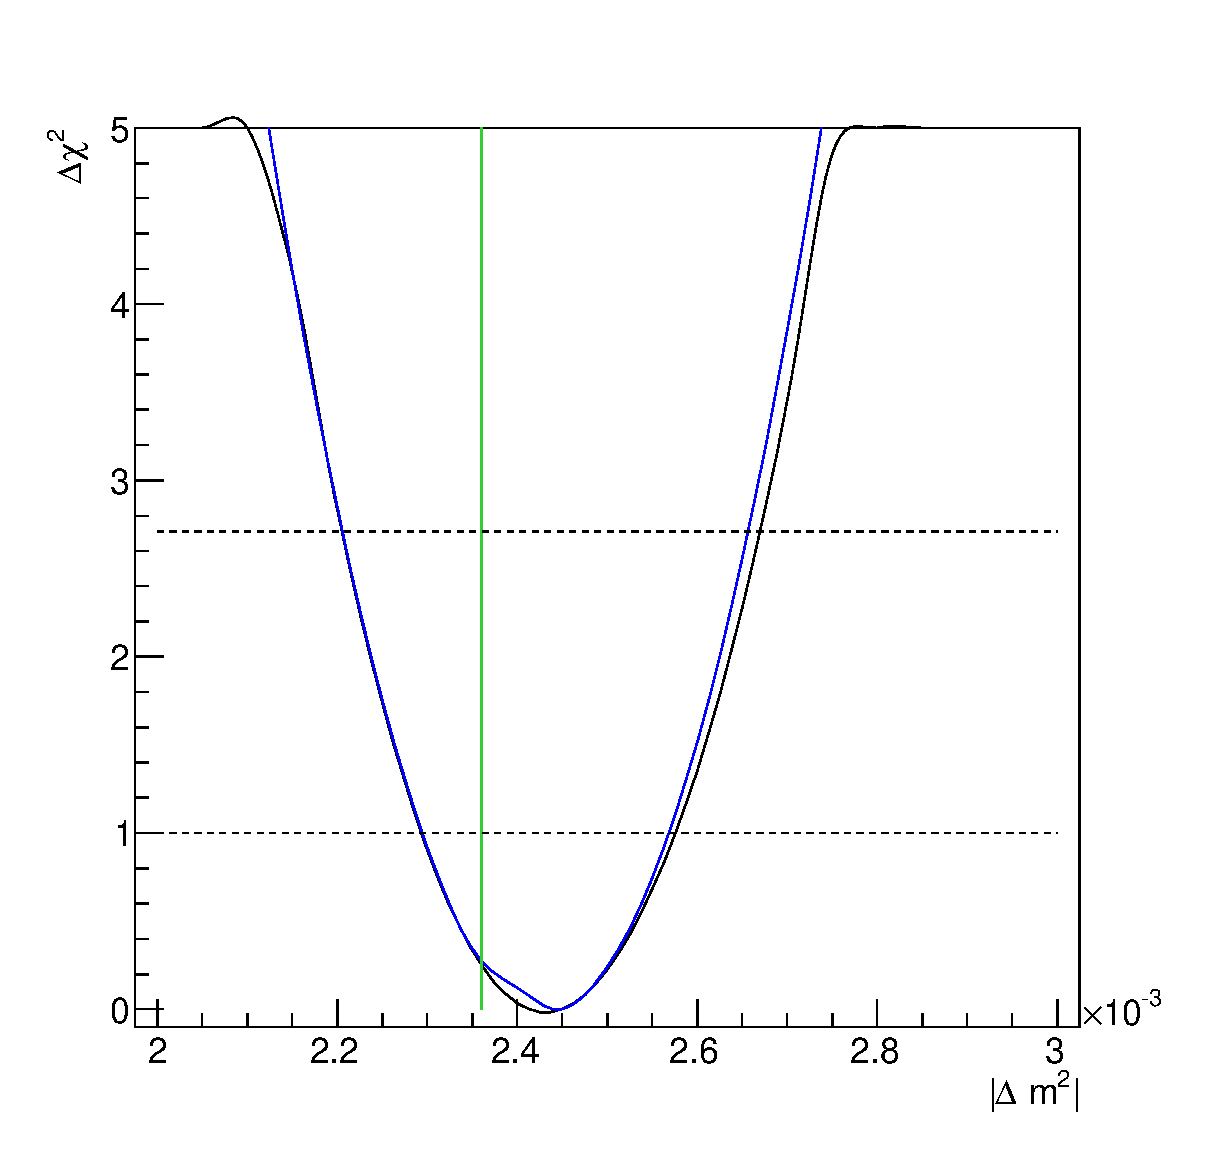
\includegraphics[width=9pc]{./images/appendix/fake_dataset_fits/realistic_fake_dataset7_chisq_dm23sq_global_min.eps}
\caption {
  $\Delta\chi^2$ as function of $|\Delta m^{2}|$ for fake dataset \#8.
  At each point, $\chi^2$ was minimized with respect to 
  $\sin^{2}\theta_{23}$, $\sin^{2}\theta_{13}$, $\delta_{CP}$
  and all relevant nuisance parameters for the joint analysis (black)
  and with respect to $\sin^{2}\theta_{23}$ and all relevant nuisance
  parameters for the disappearance analysis (blue).
}
\label{fig:toymc8_dchisq_Dmsq}
\end{minipage}
\hspace{0.02\linewidth}
\begin{minipage}[t]{0.22\linewidth}
\center
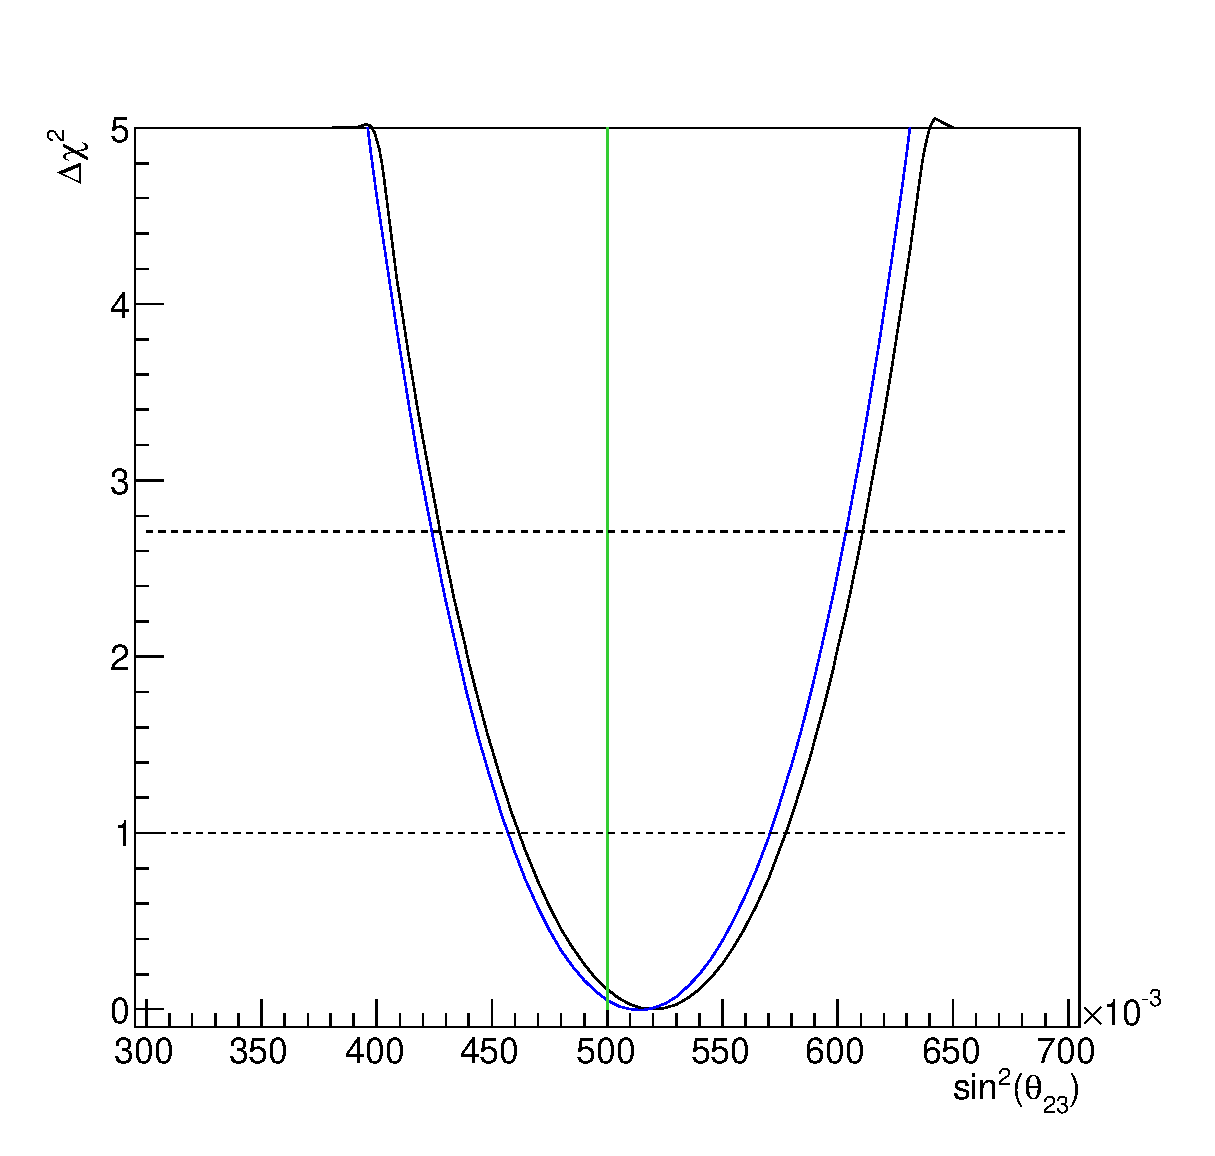
\includegraphics[width=9pc]{./images/appendix/fake_dataset_fits/realistic_fake_dataset7_chisq_theta23_global_min.eps}
\caption {
  $\Delta\chi^2$ as function of $sin^{2}\theta_{23}$ for fake dataset \#8.
  At each point, $\chi^2$ was minimized with respect to 
  $|\Delta m^{2}|$, $\sin^{2}\theta_{13}$, $\delta_{CP}$
  and all relevant nuisance parameters for the joint analysis (black)
  and with respect to $\sin^{2}\theta_{23}$ and all relevant nuisance
  parameters for the disappearance analysis (blue).
}
\label{fig:toymc8_dchisq_sinsqtheta23}
\end{minipage}
\hspace{0.02\linewidth}
\begin{minipage}[t]{0.22\linewidth}
\center
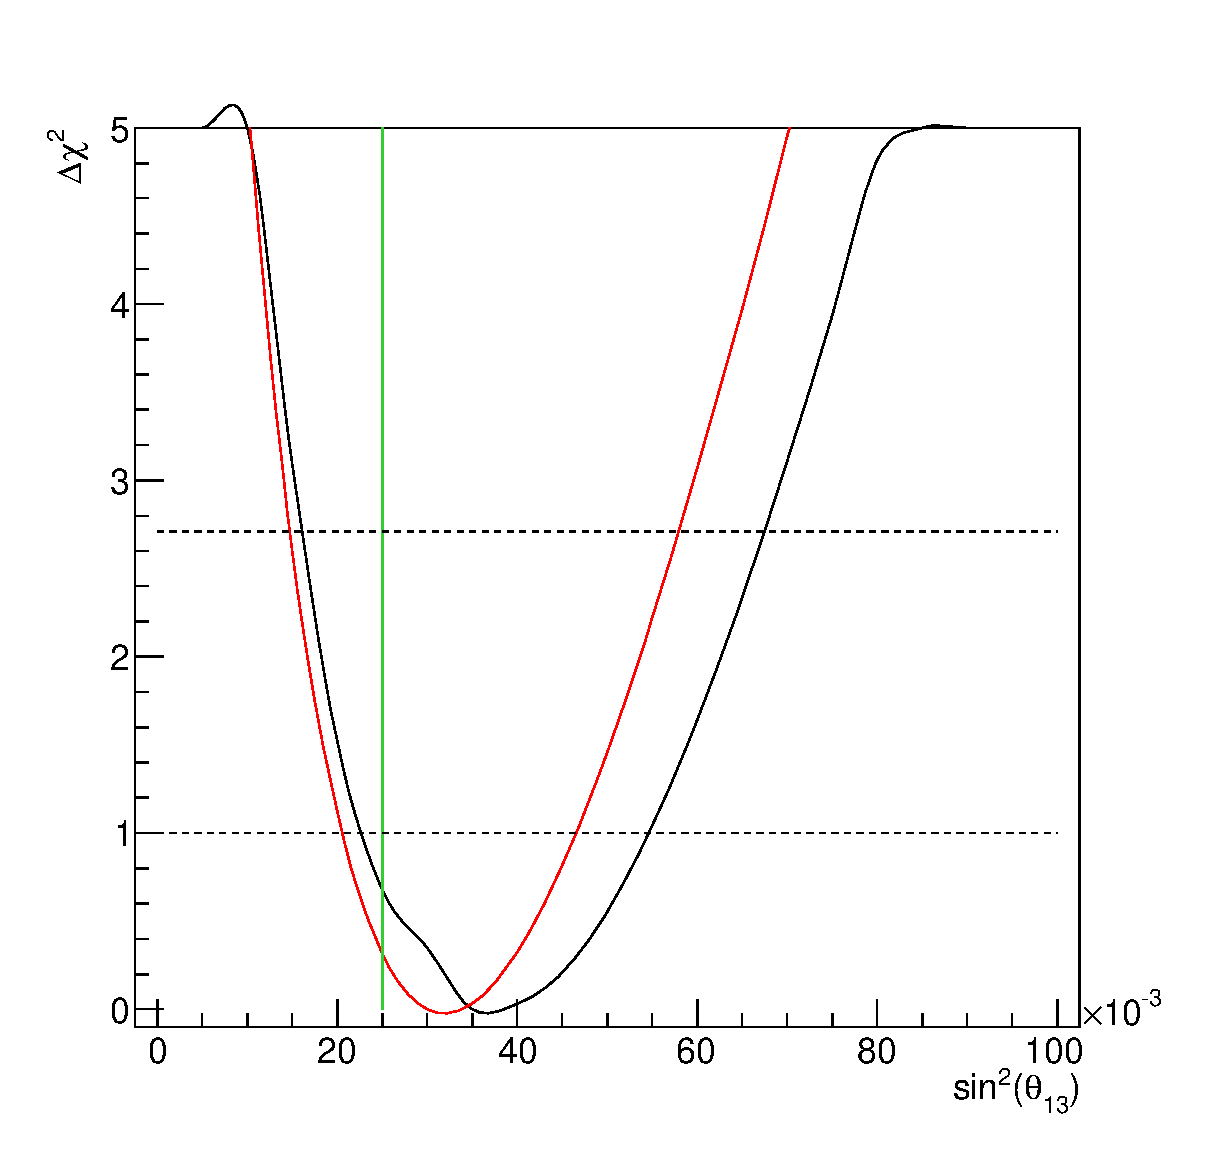
\includegraphics[width=9pc]{./images/appendix/fake_dataset_fits/realistic_fake_dataset7_chisq_theta13_global_min.eps}
\caption {
  $\Delta\chi^2$ as function of $sin^{2}\theta_{13}$ for fake dataset \#8.
  At each point, $\chi^2$ was minimized with respect to 
  $\sin^{2}\theta_{23}$, $\sin^{2}\theta_{13}$, $\delta_{CP}$
  and all relevant nuisance parameters for the joint analysis (black)
  and with respect to all relevant nuisance parameters 
  ($\delta_{CP}$ is fixed to 0) for the appearance analysis (red).
}
\label{fig:toymc8_dchisq_sinsqtheta13}
\end{minipage}
\hspace{0.02\linewidth}
\begin{minipage}[t]{0.22\linewidth}
\center
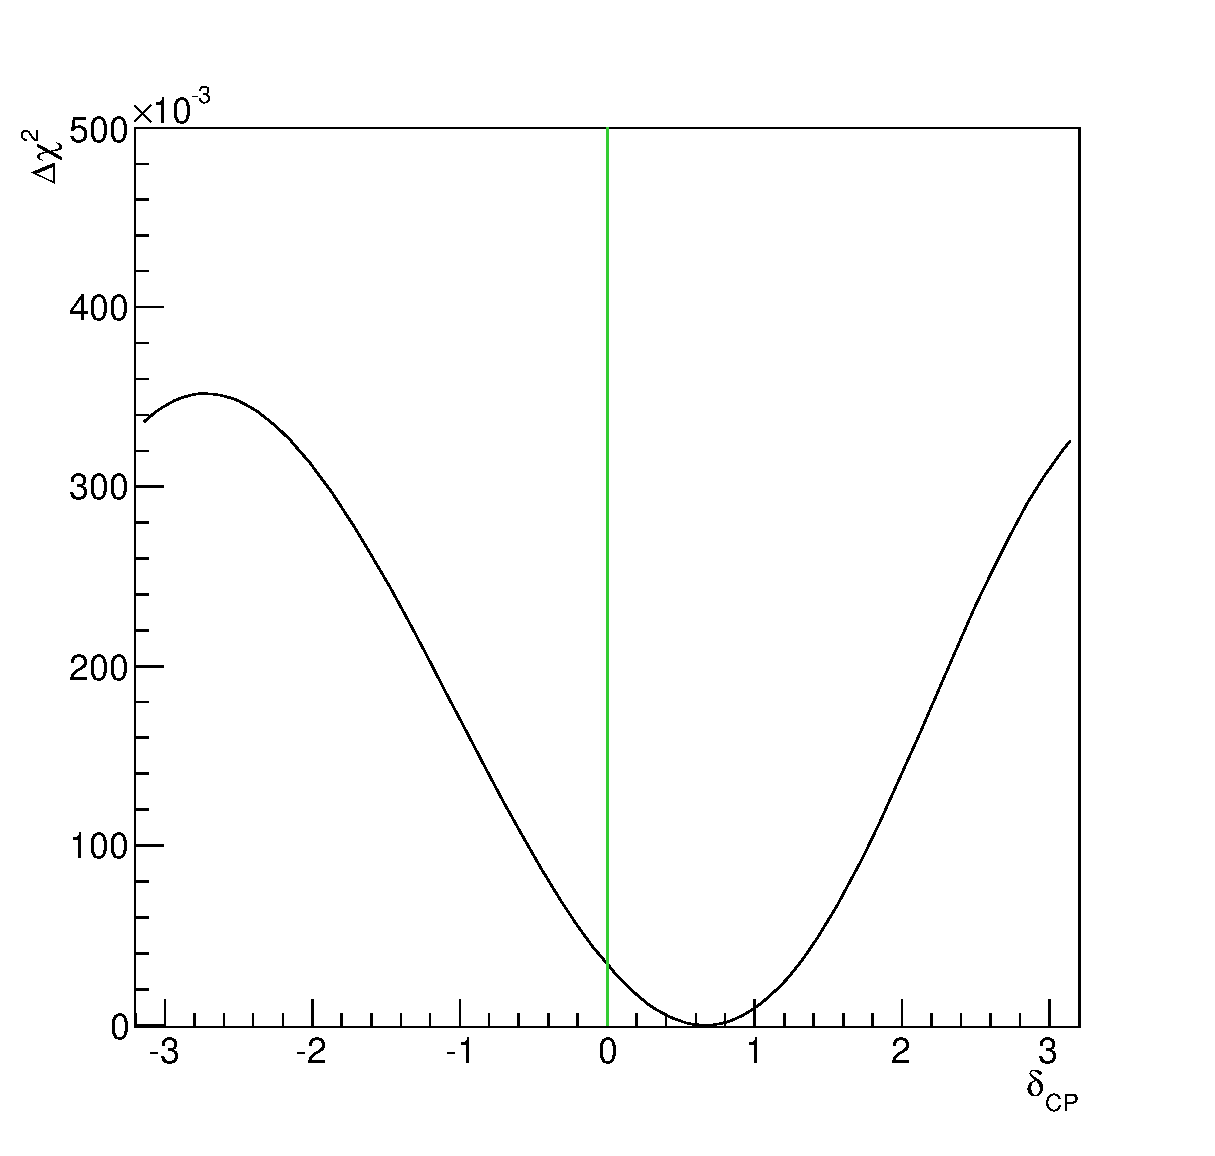
\includegraphics[width=9pc]{.//images/appendix/fake_dataset_fits/realistic_fake_dataset7_chisq_deltacp_global_min.eps}
\caption {
  $\Delta\chi^2$ as function of $\delta_{CP}$ for fake dataset \#8.
  At each point, $\chi^2$ was minimized with respect to 
  all oscillation parameters not shown (and not considered to be fixed)
  and all relevant nuisance parameters.
}
\label{fig:toymc8_dchisq_deltacp}
\end{minipage}
\vfill
\vspace*{0.7cm}
\begin{minipage}[t]{0.48\linewidth}
\center
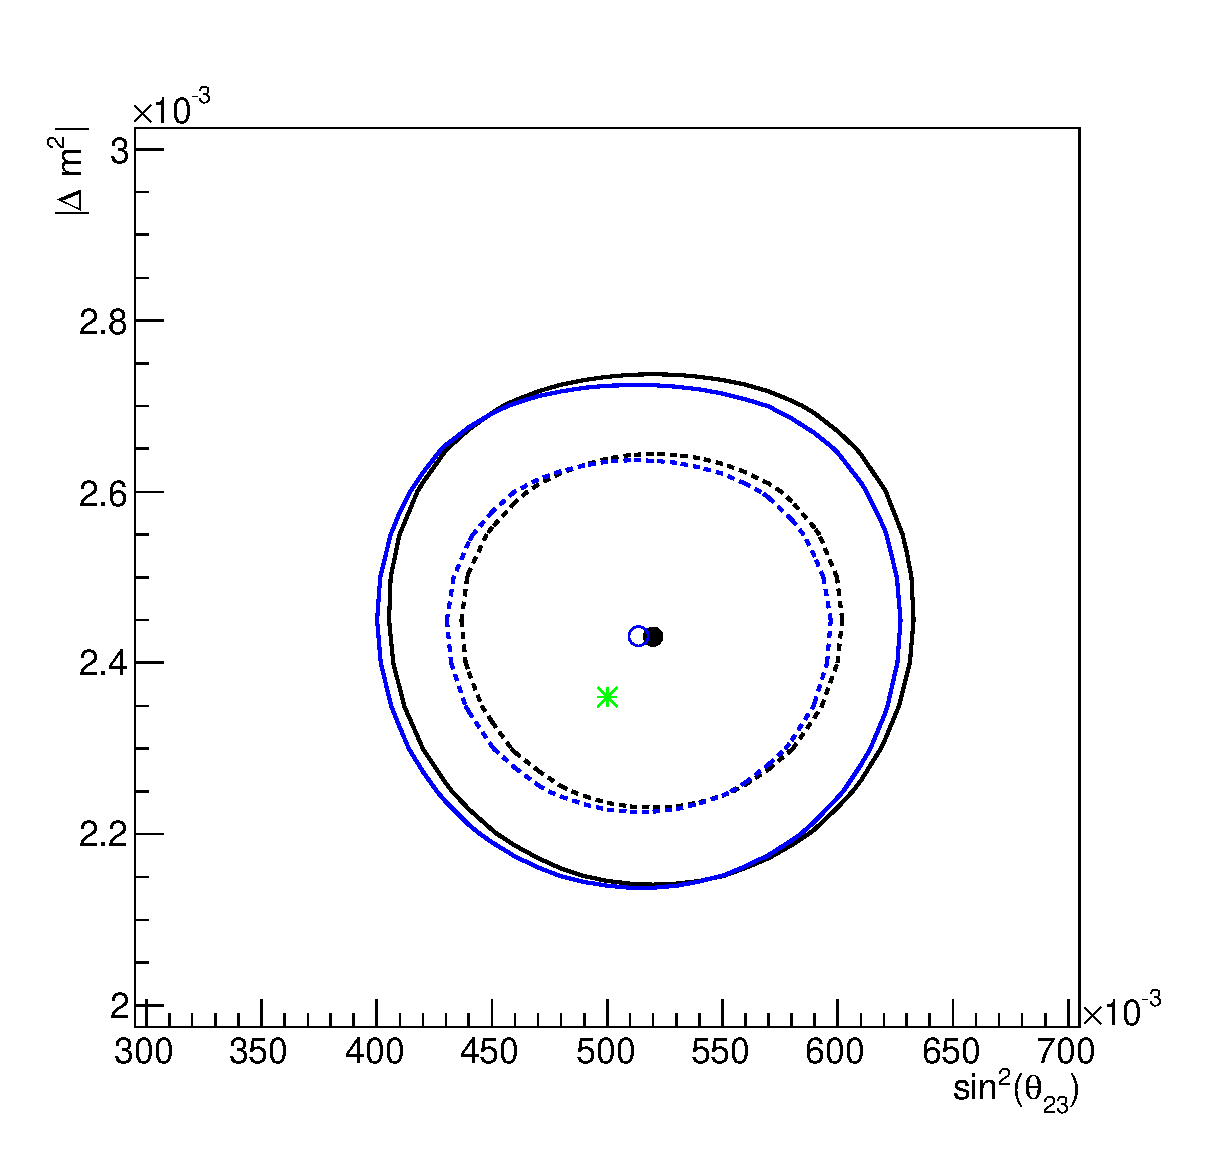
\includegraphics[width=15pc]{./images/appendix/fake_dataset_fits/realistic_fake_dataset7_chisq_theta23_dm23sq_global_min.eps}
\caption {
  68\% and 90\% CL regions in ($sin^{2}\theta_{23}$, $|\Delta m^{2}|$) space for fake dataset \#8.
  At each point, $\chi^2$ was minimized with respect to 
  $\sin^{2}\theta_{13}$, $\delta_{CP}$
  and all relevant nuisance parameters for the joint analysis (black)
  and with respect to all relevant nuisance parameters for the disappearance analysis (blue).
}
\label{fig:toymc8_confreg_sinsqtheta23_Dmsq}
\end{minipage}
\hspace{0.03\linewidth}
\begin{minipage}[t]{0.48\linewidth}
\center
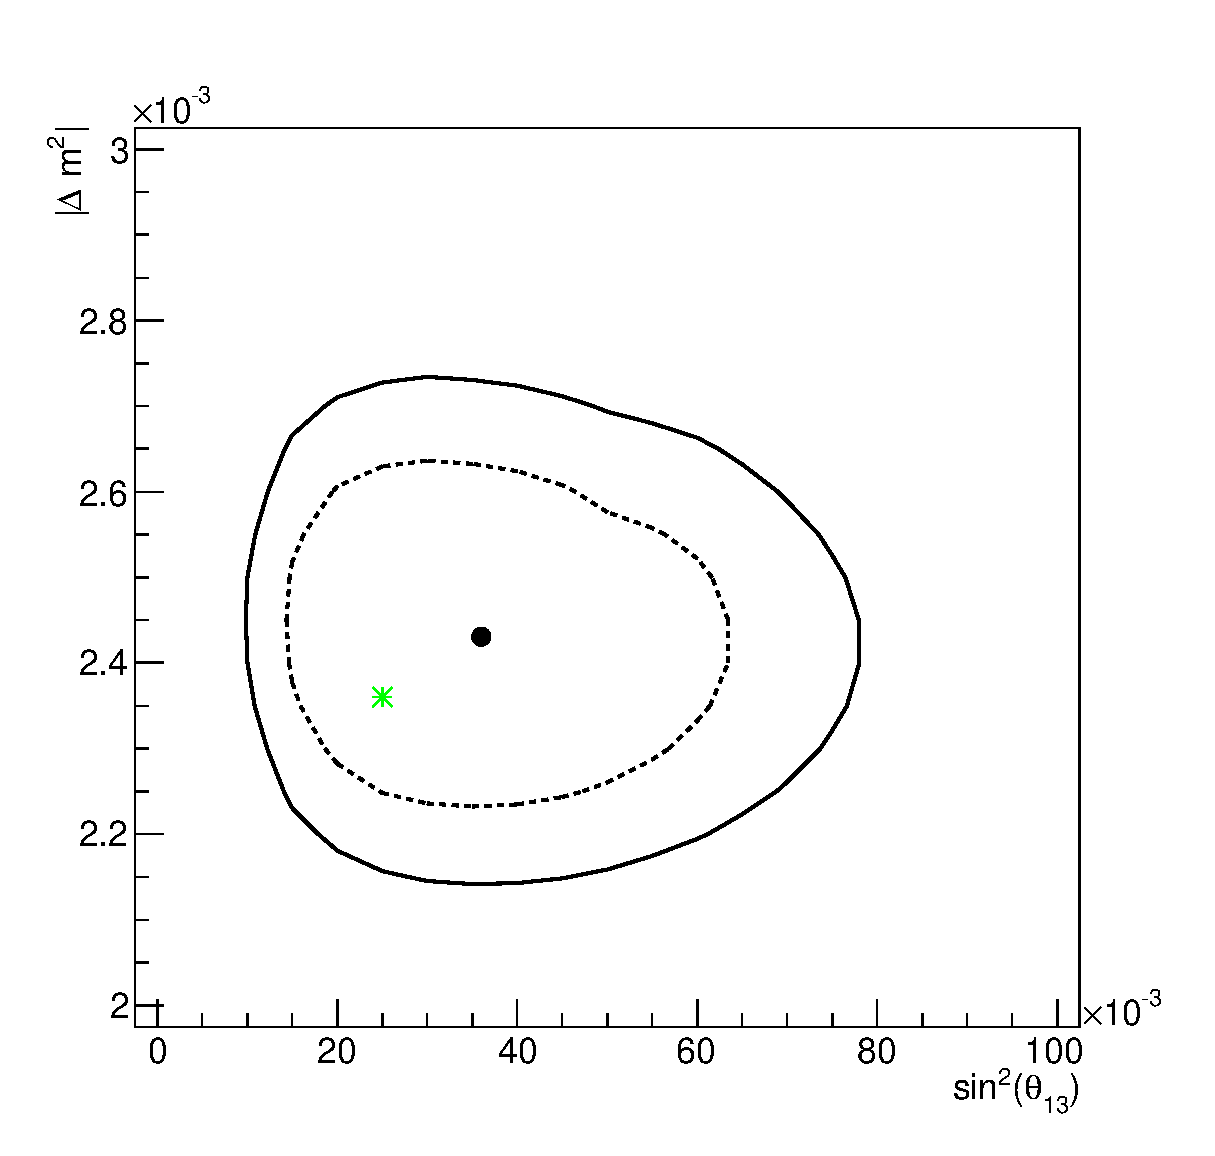
\includegraphics[width=15pc]{./images/appendix/fake_dataset_fits/realistic_fake_dataset7_chisq_theta13_dm23sq_global_min.eps}
\caption {
  68\% and 90\% CL regions in ($sin^{2}\theta_{13}$, $|\Delta m^{2}|$) space for fake dataset \#8.
  At each point, $\chi^2$ was minimized with respect to 
  all oscillation parameters not shown (and not considered to be fixed)
  and all relevant nuisance parameters.
}
\label{fig:toymc8_confreg_sinsqtheta13_Dmsq}
\end{minipage}

\vfill
\vspace*{0.7cm}

\begin{minipage}[t]{0.48\linewidth}
\center
\includegraphics[width=15pc]{./images/appendix/fake_dataset_fits/realistic_fake_dataset7_chisq_theta13_deltacp_global_min.eps}
\caption {
  68\% and 90\% CL regions in ($sin^{2}\theta_{13}$, $\delta_{CP}$) space for fake dataset \#8.
  At each point, $\chi^2$ was minimized with respect to 
  $|\Delta m^{2}|$, $\sin^{2}\theta_{23}$
  and all relevant nuisance parameters for the joint analysis (black)
  and with respect to all relevant nuisance parameters for the appearance analysis (red).
  Notice that different methods are used to
  construct confidence regions for the joint analysis (global minimum) and for the 
  stand-alone appearance analysis (raster scan).
}
\label{fig:toymc8_confreg_sinsqtheta13_deltacp}
\end{minipage}
\hspace{0.03\linewidth}
\begin{minipage}[t]{0.48\linewidth}
\center
\includegraphics[width=15pc]{./images/appendix/fake_dataset_fits/realistic_fake_dataset7_chisq_theta13_theta23_global_min.eps}
\caption {
  68\% and 90\% CL regions in ($sin^{2}\theta_{23}$, $sin^{2}\theta_{13}$) space for fake dataset \#8.
  At each point, $\chi^2$ was minimized with respect to 
  all oscillation parameters not shown (and not considered to be fixed)
  and all relevant nuisance parameters.
}
\label{fig:toymc8_confreg_sinsqtheta23_sinsqtheta13}
\end{minipage}

\end{figure*}




% 
% 
% ..............................................
% Fake dataset #9
% 
%

\clearpage
\begin{figure*}[htb]

\begin{minipage}[t]{0.46\linewidth}
\center
\includegraphics[width=15pc]{./images/appendix/fake_dataset_fits/realistic_fake_dataset2_nh_1st_1Rmu.eps}
\caption {
  Single $\mu$-like ring event best-fit reconstructed energy spectrum
  to fake dataset \#9.
}
\label{fig:toymc9_1Rmu_bestfit_spectrum}
\end{minipage}
\hspace{0.03\linewidth}
\begin{minipage}[t]{0.46\linewidth}
\center
\includegraphics[width=15pc]{./images/appendix/fake_dataset_fits/realistic_fake_dataset2_nh_1st_1Re.eps}
\caption {
  Single e-like ring event best-fit reconstructed energy spectrum
  to fake dataset \#9.
}
\label{fig:toymc9_1Re_bestfit_spectrum}
\end{minipage}

\vfill
\vspace*{0.7cm}

\begin{minipage}[t]{0.90\linewidth}
\center
\includegraphics[width=30pc,angle=270]{./images/appendix/fake_dataset_fits/pulls_realistic_fake_dataset2_nh_1st.eps}
\caption {
  Systematic parameter pulls for the oscillation fit to fake dataset \#9.
}
\label{fig:toymc9_pulls}
\end{minipage}

\end{figure*}


%...........................................................
%
% chisq distributions used for calculating the fit p-values
%

\begin{figure*}[htb]

\begin{minipage}[t]{0.90\linewidth}
\center
\includegraphics[width=30pc]{./images/appendix/fake_dataset_fits/realistic_fake_dataset2_nh_1st_gof_new.eps}
\caption {
  Distribution of $\chi^2_{gof}$, the goodness-of-fit (gof) $\chi^2$, 
  from 1k toy MC experiments generated at dataset \#9 joint 3-flavour analysis best-fit oscillation point.
  The $\chi^2_{gof}$ value for the dataset \#9 ($\chi^2_{data}$) is highlighted.
  All $\chi^2_{gof}$ values were computed 
  using the 5 (single $\mu$-like ring) + 3 (single e-like ring) 
  reconstructed energy binning scheme described in Sec.\ \ref{sec:goodness_of_fit}.
}
\label{fig:toymc9_gofchisq}
\end{minipage}

\vfill
\vspace*{0.7cm}

\begin{minipage}[t]{0.46\linewidth}
\center
\includegraphics[width=18pc]{./images/appendix/fake_dataset_fits/realistic_fake_dataset2_nh_1st_gof_disap_new.eps}
\caption {
  Distribution of $\chi^2_{gof}$
  from 1k toy MC experiments generated at the dataset \#9 stand-alone 3-flavour $\nu_{\mu}$ disappearance analysis best-fit oscillation point.
  The $\chi^2_{gof}$ value for the dataset \#9 ($\chi^2_{data}$) is highlighted.
  All $\chi^2_{gof}$ values were computed 
  using the 5 (single $\mu$-like ring) 
  reconstructed energy binning scheme described in Sec.\ \ref{sec:goodness_of_fit}.
}
\label{fig:toymc9_gofchisq_disapp}
\end{minipage}
\hspace{0.03\linewidth}
\begin{minipage}[t]{0.46\linewidth}
\center
\includegraphics[width=18pc]{./images/appendix/fake_dataset_fits/realistic_fake_dataset2_nh_1st_gof_app_new.eps}
\caption {
  Distribution of $\chi^2_{gof}$
  from 1k toy MC experiments generated at the dataset \#9 stand-alone 3-flavour $\nu_{e}$ appearance analysis best-fit oscillation point.
  The $\chi^2_{gof}$ value for the dataset \#9 ($\chi^2_{data}$) is highlighted.
  All $\chi^2_{gof}$ values were computed 
  using the 3 (single e-like ring) 
  reconstructed energy binning scheme  as described in Sec.\ \ref{sec:goodness_of_fit}.
  }
\label{fig:toymc9_gofchisq_app}
\end{minipage}

\end{figure*}



%
% delta\chisq and contours
%

\begin{figure*}[htb]

\begin{minipage}[t]{0.22\linewidth}
\center
\includegraphics[width=9pc]{./images/appendix/fake_dataset_fits/realistic_fake_dataset2_chisq_dm23sq_global_min.eps}
\caption {
  $\Delta\chi^2$ as function of $|\Delta m^{2}|$ for fake dataset \#9.
  At each point, $\chi^2$ was minimized with respect to 
  $\sin^{2}\theta_{23}$, $\sin^{2}\theta_{13}$, $\delta_{CP}$
  and all relevant nuisance parameters for the joint analysis (black)
  and with respect to $\sin^{2}\theta_{23}$ and all relevant nuisance
  parameters for the disappearance analysis (blue).
}
\label{fig:toymc9_dchisq_Dmsq}
\end{minipage}
\hspace{0.02\linewidth}
\begin{minipage}[t]{0.22\linewidth}
\center
\includegraphics[width=9pc]{./images/appendix/fake_dataset_fits/realistic_fake_dataset2_chisq_theta23_global_min.eps}
\caption {
  $\Delta\chi^2$ as function of $sin^{2}\theta_{23}$ for fake dataset \#9.
  At each point, $\chi^2$ was minimized with respect to 
  $|\Delta m^{2}|$, $\sin^{2}\theta_{13}$, $\delta_{CP}$
  and all relevant nuisance parameters for the joint analysis (black)
  and with respect to $\sin^{2}\theta_{23}$ and all relevant nuisance
  parameters for the disappearance analysis (blue).
}
\label{fig:toymc9_dchisq_sinsqtheta23}
\end{minipage}
\hspace{0.02\linewidth}
\begin{minipage}[t]{0.22\linewidth}
\center
\includegraphics[width=9pc]{./images/appendix/fake_dataset_fits/realistic_fake_dataset2_chisq_theta13_global_min.eps}
\caption {
  $\Delta\chi^2$ as function of $sin^{2}\theta_{13}$ for fake dataset \#9.
  At each point, $\chi^2$ was minimized with respect to 
  $\sin^{2}\theta_{23}$, $\sin^{2}\theta_{13}$, $\delta_{CP}$
  and all relevant nuisance parameters for the joint analysis (black)
  and with respect to all relevant nuisance parameters 
  ($\delta_{CP}$ is fixed to 0) for the appearance analysis (red).
}
\label{fig:toymc9_dchisq_sinsqtheta13}
\end{minipage}
\hspace{0.02\linewidth}
\begin{minipage}[t]{0.22\linewidth}
\center
\includegraphics[width=9pc]{.//images/appendix/fake_dataset_fits/realistic_fake_dataset2_chisq_deltacp_global_min.eps}
\caption {
  $\Delta\chi^2$ as function of $\delta_{CP}$ for fake dataset \#9.
  At each point, $\chi^2$ was minimized with respect to 
  all oscillation parameters not shown (and not considered to be fixed)
  and all relevant nuisance parameters.
}
\label{fig:toymc9_dchisq_deltacp}
\end{minipage}
\vfill
\vspace*{0.7cm}
\begin{minipage}[t]{0.48\linewidth}
\center
\includegraphics[width=15pc]{./images/appendix/fake_dataset_fits/realistic_fake_dataset2_chisq_theta23_dm23sq_global_min.eps}
\caption {
  68\% and 90\% CL regions in ($sin^{2}\theta_{23}$, $|\Delta m^{2}|$) space for fake dataset \#9.
  At each point, $\chi^2$ was minimized with respect to 
  $\sin^{2}\theta_{13}$, $\delta_{CP}$
  and all relevant nuisance parameters for the joint analysis (black)
  and with respect to all relevant nuisance parameters for the disappearance analysis (blue).
}
\label{fig:toymc9_confreg_sinsqtheta23_Dmsq}
\end{minipage}
\hspace{0.03\linewidth}
\begin{minipage}[t]{0.48\linewidth}
\center
\includegraphics[width=15pc]{./images/appendix/fake_dataset_fits/realistic_fake_dataset2_chisq_theta13_dm23sq_global_min.eps}
\caption {
  68\% and 90\% CL regions in ($sin^{2}\theta_{13}$, $|\Delta m^{2}|$) space for fake dataset \#9.
  At each point, $\chi^2$ was minimized with respect to 
  all oscillation parameters not shown (and not considered to be fixed)
  and all relevant nuisance parameters.
}
\label{fig:toymc9_confreg_sinsqtheta13_Dmsq}
\end{minipage}

\vfill
\vspace*{0.7cm}

\begin{minipage}[t]{0.48\linewidth}
\center
\includegraphics[width=15pc]{./images/appendix/fake_dataset_fits/realistic_fake_dataset2_chisq_theta13_deltacp_global_min.eps}
\caption {
  68\% and 90\% CL regions in ($sin^{2}\theta_{13}$, $\delta_{CP}$) space for fake dataset \#9.
  At each point, $\chi^2$ was minimized with respect to 
  $|\Delta m^{2}|$, $\sin^{2}\theta_{23}$
  and all relevant nuisance parameters for the joint analysis (black)
  and with respect to all relevant nuisance parameters for the appearance analysis (red).
  Notice that different methods are used to
  construct confidence regions for the joint analysis (global minimum) and for the 
  stand-alone appearance analysis (raster scan).
}
\label{fig:toymc9_confreg_sinsqtheta13_deltacp}
\end{minipage}
\hspace{0.03\linewidth}
\begin{minipage}[t]{0.48\linewidth}
\center
\includegraphics[width=15pc]{./images/appendix/fake_dataset_fits/realistic_fake_dataset2_chisq_theta13_theta23_global_min.eps}
\caption {
  68\% and 90\% CL regions in ($sin^{2}\theta_{23}$, $sin^{2}\theta_{13}$) space for fake dataset \#9.
  At each point, $\chi^2$ was minimized with respect to 
  all oscillation parameters not shown (and not considered to be fixed)
  and all relevant nuisance parameters.
}
\label{fig:toymc9_confreg_sinsqtheta23_sinsqtheta13}
\end{minipage}

\end{figure*}





% 
% 
% ..............................................
% Fake dataset #10
% 
%

\clearpage
\begin{figure*}[htb]

\begin{minipage}[t]{0.46\linewidth}
\center
\includegraphics[width=15pc]{./images/appendix/fake_dataset_fits/realistic_fake_dataset3_nh_1st_1Rmu.eps}
\caption {
  Single $\mu$-like ring event best-fit reconstructed energy spectrum
  to fake dataset \#10.
}
\label{fig:toymc10_1Rmu_bestfit_spectrum}
\end{minipage}
\hspace{0.03\linewidth}
\begin{minipage}[t]{0.46\linewidth}
\center
\includegraphics[width=15pc]{./images/appendix/fake_dataset_fits/realistic_fake_dataset3_nh_1st_1Re.eps}
\caption {
  Single e-like ring event best-fit reconstructed energy spectrum
  to fake dataset \#10.
}
\label{fig:toymc10_1Re_bestfit_spectrum}
\end{minipage}

\vfill
\vspace*{0.7cm}

\begin{minipage}[t]{0.90\linewidth}
\center
\includegraphics[width=30pc,angle=270]{./images/appendix/fake_dataset_fits/pulls_realistic_fake_dataset3_nh_1st.eps}
\caption {
  Systematic parameter pulls for the oscillation fit to fake dataset \#10.
}
\label{fig:toymc10_pulls}
\end{minipage}

\end{figure*}


%...........................................................
%
% chisq distributions used for calculating the fit p-values
%

\begin{figure*}[htb]

\begin{minipage}[t]{0.90\linewidth}
\center
\includegraphics[width=30pc]{./images/appendix/fake_dataset_fits/realistic_fake_dataset3_nh_1st_gof_new.eps}
\caption {
  Distribution of $\chi^2_{gof}$, the goodness-of-fit (gof) $\chi^2$, 
  from 1k toy MC experiments generated at dataset \#10 joint 3-flavour analysis best-fit oscillation point.
  The $\chi^2_{gof}$ value for the dataset \#10 ($\chi^2_{data}$) is highlighted.
  All $\chi^2_{gof}$ values were computed 
  using the 5 (single $\mu$-like ring) + 3 (single e-like ring) 
  reconstructed energy binning scheme described in Sec.\ \ref{sec:goodness_of_fit}.
}
\label{fig:toymc10_gofchisq}
\end{minipage}

\vfill
\vspace*{0.7cm}

\begin{minipage}[t]{0.46\linewidth}
\center
\includegraphics[width=18pc]{./images/appendix/fake_dataset_fits/realistic_fake_dataset3_nh_1st_gof_disap_new.eps}
\caption {
  Distribution of $\chi^2_{gof}$
  from 1k toy MC experiments generated at the dataset \#10 stand-alone 3-flavour $\nu_{\mu}$ disappearance analysis best-fit oscillation point.
  The $\chi^2_{gof}$ value for the dataset \#10 ($\chi^2_{data}$) is highlighted.
  All $\chi^2_{gof}$ values were computed 
  using the 5 (single $\mu$-like ring) 
  reconstructed energy binning scheme described in Sec.\ \ref{sec:goodness_of_fit}.
}
\label{fig:toymc10_gofchisq_disapp}
\end{minipage}
\hspace{0.03\linewidth}
\begin{minipage}[t]{0.46\linewidth}
\center
\includegraphics[width=18pc]{./images/appendix/fake_dataset_fits/realistic_fake_dataset3_nh_1st_gof_app_new.eps}
\caption {
  Distribution of $\chi^2_{gof}$
  from 1k toy MC experiments generated at the dataset \#10 stand-alone 3-flavour $\nu_{e}$ appearance analysis best-fit oscillation point.
  The $\chi^2_{gof}$ value for the dataset \#10 ($\chi^2_{data}$) is highlighted.
  All $\chi^2_{gof}$ values were computed 
  using the 3 (single e-like ring) 
  reconstructed energy binning scheme  as described in Sec.\ \ref{sec:goodness_of_fit}.
}
\label{fig:toymc10_gofchisq_app}
\end{minipage}

\end{figure*}



%
% delta\chisq and contours
%

\begin{figure*}[htb]

\begin{minipage}[t]{0.22\linewidth}
\center
\includegraphics[width=9pc]{./images/appendix/fake_dataset_fits/realistic_fake_dataset3_chisq_dm23sq_global_min.eps}
\caption {
  $\Delta\chi^2$ as function of $|\Delta m^{2}|$ for fake dataset \#10.
  At each point, $\chi^2$ was minimized with respect to 
  $\sin^{2}\theta_{23}$, $\sin^{2}\theta_{13}$, $\delta_{CP}$
  and all relevant nuisance parameters for the joint analysis (black)
  and with respect to $\sin^{2}\theta_{23}$ and all relevant nuisance
  parameters for the disappearance analysis (blue).
}
\label{fig:toymc10_dchisq_Dmsq}
\end{minipage}
\hspace{0.02\linewidth}
\begin{minipage}[t]{0.22\linewidth}
\center
\includegraphics[width=9pc]{./images/appendix/fake_dataset_fits/realistic_fake_dataset3_chisq_theta23_global_min.eps}
\caption {
  $\Delta\chi^2$ as function of $sin^{2}\theta_{23}$ for fake dataset \#10.
  At each point, $\chi^2$ was minimized with respect to 
  $|\Delta m^{2}|$, $\sin^{2}\theta_{13}$, $\delta_{CP}$
  and all relevant nuisance parameters for the joint analysis (black)
  and with respect to $\sin^{2}\theta_{23}$ and all relevant nuisance
  parameters for the disappearance analysis (blue).
}
\label{fig:toymc10_dchisq_sinsqtheta23}
\end{minipage}
\hspace{0.02\linewidth}
\begin{minipage}[t]{0.22\linewidth}
\center
\includegraphics[width=9pc]{./images/appendix/fake_dataset_fits/realistic_fake_dataset3_chisq_theta13_global_min.eps}
\caption {
  $\Delta\chi^2$ as function of $sin^{2}\theta_{13}$ for fake dataset \#10.
  At each point, $\chi^2$ was minimized with respect to 
  $\sin^{2}\theta_{23}$, $\sin^{2}\theta_{13}$, $\delta_{CP}$
  and all relevant nuisance parameters for the joint analysis (black)
  and with respect to all relevant nuisance parameters 
  ($\delta_{CP}$ is fixed to 0) for the appearance analysis (red).
}
\label{fig:toymc10_dchisq_sinsqtheta13}
\end{minipage}
\hspace{0.02\linewidth}
\begin{minipage}[t]{0.22\linewidth}
\center
\includegraphics[width=9pc]{.//images/appendix/fake_dataset_fits/realistic_fake_dataset3_chisq_deltacp_global_min.eps}
\caption {
  $\Delta\chi^2$ as function of $\delta_{CP}$ for fake dataset \#10.
  At each point, $\chi^2$ was minimized with respect to 
  all oscillation parameters not shown (and not considered to be fixed)
  and all relevant nuisance parameters.
}
\label{fig:toymc10_dchisq_deltacp}
\end{minipage}
\vfill
\vspace*{0.7cm}
\begin{minipage}[t]{0.48\linewidth}
\center
\includegraphics[width=15pc]{./images/appendix/fake_dataset_fits/realistic_fake_dataset3_chisq_theta23_dm23sq_global_min.eps}
\caption {
  68\% and 90\% CL regions in ($sin^{2}\theta_{23}$, $|\Delta m^{2}|$) space for fake dataset \#10.
  At each point, $\chi^2$ was minimized with respect to 
  $\sin^{2}\theta_{13}$, $\delta_{CP}$
  and all relevant nuisance parameters for the joint analysis (black)
  and with respect to all relevant nuisance parameters for the disappearance analysis (blue).
}
\label{fig:toymc10_confreg_sinsqtheta23_Dmsq}
\end{minipage}
\hspace{0.03\linewidth}
\begin{minipage}[t]{0.48\linewidth}
\center
\includegraphics[width=15pc]{./images/appendix/fake_dataset_fits/realistic_fake_dataset3_chisq_theta13_dm23sq_global_min.eps}
\caption {
  68\% and 90\% CL regions in ($sin^{2}\theta_{13}$, $|\Delta m^{2}|$) space for fake dataset \#10.
  At each point, $\chi^2$ was minimized with respect to 
  all oscillation parameters not shown (and not considered to be fixed)
  and all relevant nuisance parameters.
}
\label{fig:toymc10_confreg_sinsqtheta13_Dmsq}
\end{minipage}

\vfill
\vspace*{0.7cm}

\begin{minipage}[t]{0.48\linewidth}
\center
\includegraphics[width=15pc]{./images/appendix/fake_dataset_fits/realistic_fake_dataset3_chisq_theta13_deltacp_global_min.eps}
\caption {
  68\% and 90\% CL regions in ($sin^{2}\theta_{13}$, $\delta_{CP}$) space for fake dataset \#10.
  At each point, $\chi^2$ was minimized with respect to 
  $|\Delta m^{2}|$, $\sin^{2}\theta_{23}$
  and all relevant nuisance parameters for the joint analysis (black)
  and with respect to all relevant nuisance parameters for the appearance analysis (red).
  Notice that different methods are used to
  construct confidence regions for the joint analysis (global minimum) and for the 
  stand-alone appearance analysis (raster scan).
}
\label{fig:toymc10_confreg_sinsqtheta13_deltacp}
\end{minipage}
\hspace{0.03\linewidth}
\begin{minipage}[t]{0.48\linewidth}
\center
\includegraphics[width=15pc]{./images/appendix/fake_dataset_fits/realistic_fake_dataset3_chisq_theta13_theta23_global_min.eps}
\caption {
  68\% and 90\% CL regions in ($sin^{2}\theta_{23}$, $sin^{2}\theta_{13}$) space for fake dataset \#10.
  At each point, $\chi^2$ was minimized with respect to 
  all oscillation parameters not shown (and not considered to be fixed)
  and all relevant nuisance parameters.
}
\label{fig:toymc10_confreg_sinsqtheta23_sinsqtheta13}
\end{minipage}

\end{figure*}





% 
% 
% ..............................................
% Fake dataset #11
% 
%

\clearpage
\begin{figure*}[htb]

\begin{minipage}[t]{0.46\linewidth}
\center
\includegraphics[width=15pc]{./images/appendix/fake_dataset_fits/realistic_fake_dataset4_nh_1st_1Rmu.eps}
\caption {
  Single $\mu$-like ring event best-fit reconstructed energy spectrum
  to fake dataset \#11.
}
\label{fig:toymc11_1Rmu_bestfit_spectrum}
\end{minipage}
\hspace{0.03\linewidth}
\begin{minipage}[t]{0.46\linewidth}
\center
\includegraphics[width=15pc]{./images/appendix/fake_dataset_fits/realistic_fake_dataset4_nh_1st_1Re.eps}
\caption {
  Single e-like ring event best-fit reconstructed energy spectrum
  to fake dataset \#11.
}
\label{fig:toymc11_1Re_bestfit_spectrum}
\end{minipage}

\vfill
\vspace*{0.7cm}

\begin{minipage}[t]{0.90\linewidth}
\center
\includegraphics[width=30pc,angle=270]{./images/appendix/fake_dataset_fits/pulls_realistic_fake_dataset4_nh_1st.eps}
\caption {
  Systematic parameter pulls for the oscillation fit to fake dataset \#11.
}
\label{fig:toymc11_pulls}
\end{minipage}

\end{figure*}


%...........................................................
%
% chisq distributions used for calculating the fit p-values
%

\begin{figure*}[htb]

\begin{minipage}[t]{0.90\linewidth}
\center
\includegraphics[width=30pc]{./images/appendix/fake_dataset_fits/realistic_fake_dataset4_nh_1st_gof_new.eps}
\caption {
  Distribution of $\chi^2_{gof}$, the goodness-of-fit (gof) $\chi^2$, 
  from 1k toy MC experiments generated at dataset \#11 joint 3-flavour analysis best-fit oscillation point.
  The $\chi^2_{gof}$ value for the dataset \#11 ($\chi^2_{data}$) is highlighted.
  All $\chi^2_{gof}$ values were computed 
  using the 5 (single $\mu$-like ring) + 3 (single e-like ring) 
  reconstructed energy binning scheme described in Sec.\ \ref{sec:goodness_of_fit}.
}
\label{fig:toymc11_gofchisq}
\end{minipage}

\vfill
\vspace*{0.7cm}

\begin{minipage}[t]{0.46\linewidth}
\center
\includegraphics[width=18pc]{./images/appendix/fake_dataset_fits/realistic_fake_dataset4_nh_1st_gof_disap_new.eps}
\caption {
  Distribution of $\chi^2_{gof}$
  from 1k toy MC experiments generated at the dataset \#11 stand-alone 3-flavour $\nu_{\mu}$ disappearance analysis best-fit oscillation point.
  The $\chi^2_{gof}$ value for the dataset \#11 ($\chi^2_{data}$) is highlighted.
  All $\chi^2_{gof}$ values were computed 
  using the 5 (single $\mu$-like ring) 
  reconstructed energy binning scheme described in Sec.\ \ref{sec:goodness_of_fit}.
}
\label{fig:toymc11_gofchisq_disapp}
\end{minipage}
\hspace{0.03\linewidth}
\begin{minipage}[t]{0.46\linewidth}
\center
\includegraphics[width=18pc]{./images/appendix/fake_dataset_fits/realistic_fake_dataset4_nh_1st_gof_app_new.eps}
\caption {
  Distribution of $\chi^2_{gof}$
  from 1k toy MC experiments generated at the dataset \#11 stand-alone 3-flavour $\nu_{e}$ appearance analysis best-fit oscillation point.
  The $\chi^2_{gof}$ value for the dataset \#11 ($\chi^2_{data}$) is highlighted.
  All $\chi^2_{gof}$ values were computed 
  using the 3 (single e-like ring) 
  reconstructed energy binning scheme  as described in Sec.\ \ref{sec:goodness_of_fit}.
}
\label{fig:toymc11_gofchisq_app}
\end{minipage}

\end{figure*}



%
% delta\chisq and contours
%

\begin{figure*}[htb]

\begin{minipage}[t]{0.22\linewidth}
\center
\includegraphics[width=9pc]{./images/appendix/fake_dataset_fits/realistic_fake_dataset4_chisq_dm23sq_global_min.eps}
\caption {
  $\Delta\chi^2$ as function of $|\Delta m^{2}|$ for fake dataset \#11.
  At each point, $\chi^2$ was minimized with respect to 
  $\sin^{2}\theta_{23}$, $\sin^{2}\theta_{13}$, $\delta_{CP}$
  and all relevant nuisance parameters for the joint analysis (black)
  and with respect to $\sin^{2}\theta_{23}$ and all relevant nuisance
  parameters for the disappearance analysis (blue).
}
\label{fig:toymc11_dchisq_Dmsq}
\end{minipage}
\hspace{0.02\linewidth}
\begin{minipage}[t]{0.22\linewidth}
\center
\includegraphics[width=9pc]{./images/appendix/fake_dataset_fits/realistic_fake_dataset4_chisq_theta23_global_min.eps}
\caption {
  $\Delta\chi^2$ as function of $sin^{2}\theta_{23}$ for fake dataset \#11.
  At each point, $\chi^2$ was minimized with respect to 
  $|\Delta m^{2}|$, $\sin^{2}\theta_{13}$, $\delta_{CP}$
  and all relevant nuisance parameters for the joint analysis (black)
  and with respect to $\sin^{2}\theta_{23}$ and all relevant nuisance
  parameters for the disappearance analysis (blue).
}
\label{fig:toymc11_dchisq_sinsqtheta23}
\end{minipage}
\hspace{0.02\linewidth}
\begin{minipage}[t]{0.22\linewidth}
\center
\includegraphics[width=9pc]{./images/appendix/fake_dataset_fits/realistic_fake_dataset4_chisq_theta13_global_min.eps}
\caption {
  $\Delta\chi^2$ as function of $sin^{2}\theta_{13}$ for fake dataset \#11.
  At each point, $\chi^2$ was minimized with respect to 
  $\sin^{2}\theta_{23}$, $\sin^{2}\theta_{13}$, $\delta_{CP}$
  and all relevant nuisance parameters for the joint analysis (black)
  and with respect to all relevant nuisance parameters 
  ($\delta_{CP}$ is fixed to 0) for the appearance analysis (red).
}
\label{fig:toymc11_dchisq_sinsqtheta13}
\end{minipage}
\hspace{0.02\linewidth}
\begin{minipage}[t]{0.22\linewidth}
\center
\includegraphics[width=9pc]{.//images/appendix/fake_dataset_fits/realistic_fake_dataset4_chisq_deltacp_global_min.eps}
\caption {
  $\Delta\chi^2$ as function of $\delta_{CP}$ for fake dataset \#11.
  At each point, $\chi^2$ was minimized with respect to 
  all oscillation parameters not shown (and not considered to be fixed)
  and all relevant nuisance parameters.
}
\label{fig:toymc11_dchisq_deltacp}
\end{minipage}
\vfill
\vspace*{0.7cm}
\begin{minipage}[t]{0.48\linewidth}
\center
\includegraphics[width=15pc]{./images/appendix/fake_dataset_fits/realistic_fake_dataset4_chisq_theta23_dm23sq_global_min.eps}
\caption {
  68\% and 90\% CL regions in ($sin^{2}\theta_{23}$, $|\Delta m^{2}|$) space for fake dataset \#11.
  At each point, $\chi^2$ was minimized with respect to 
  $\sin^{2}\theta_{13}$, $\delta_{CP}$
  and all relevant nuisance parameters for the joint analysis (black)
  and with respect to all relevant nuisance parameters for the disappearance analysis (blue).
}
\label{fig:toymc11_confreg_sinsqtheta23_Dmsq}
\end{minipage}
\hspace{0.03\linewidth}
\begin{minipage}[t]{0.48\linewidth}
\center
\includegraphics[width=15pc]{./images/appendix/fake_dataset_fits/realistic_fake_dataset4_chisq_theta13_dm23sq_global_min.eps}
\caption {
  68\% and 90\% CL regions in ($sin^{2}\theta_{13}$, $|\Delta m^{2}|$) space for fake dataset \#11.
  At each point, $\chi^2$ was minimized with respect to 
  all oscillation parameters not shown (and not considered to be fixed)
  and all relevant nuisance parameters.
}
\label{fig:toymc11_confreg_sinsqtheta13_Dmsq}
\end{minipage}

\vfill
\vspace*{0.7cm}

\begin{minipage}[t]{0.48\linewidth}
\center
\includegraphics[width=15pc]{./images/appendix/fake_dataset_fits/realistic_fake_dataset4_chisq_theta13_deltacp_global_min.eps}
\caption {
  68\% and 90\% CL regions in ($sin^{2}\theta_{13}$, $\delta_{CP}$) space for fake dataset \#11.
  At each point, $\chi^2$ was minimized with respect to 
  $|\Delta m^{2}|$, $\sin^{2}\theta_{23}$
  and all relevant nuisance parameters for the joint analysis (black)
  and with respect to all relevant nuisance parameters for the appearance analysis (red).
  Notice that different methods are used to
  construct confidence regions for the joint analysis (global minimum) and for the 
  stand-alone appearance analysis (raster scan).
}
\label{fig:toymc11_confreg_sinsqtheta13_deltacp}
\end{minipage}
\hspace{0.03\linewidth}
\begin{minipage}[t]{0.48\linewidth}
\center
\includegraphics[width=15pc]{./images/appendix/fake_dataset_fits/realistic_fake_dataset4_chisq_theta13_theta23_global_min.eps}
\caption {
  68\% and 90\% CL regions in ($sin^{2}\theta_{23}$, $sin^{2}\theta_{13}$) space for fake dataset \#11.
  At each point, $\chi^2$ was minimized with respect to 
  all oscillation parameters not shown (and not considered to be fixed)
  and all relevant nuisance parameters.
}
\label{fig:toymc11_confreg_sinsqtheta23_sinsqtheta13}
\end{minipage}

\end{figure*}



% 
% 
% ..............................................
% Fake dataset #12
% 
%

\clearpage
\begin{figure*}[htb]

\begin{minipage}[t]{0.46\linewidth}
\center
\includegraphics[width=15pc]{./images/appendix/fake_dataset_fits/realistic_fake_dataset5_nh_1st_1Rmu.eps}
\caption {
  Single $\mu$-like ring event best-fit reconstructed energy spectrum
  to fake dataset \#12.
}
\label{fig:toymc12_1Rmu_bestfit_spectrum}
\end{minipage}
\hspace{0.03\linewidth}
\begin{minipage}[t]{0.46\linewidth}
\center
\includegraphics[width=15pc]{./images/appendix/fake_dataset_fits/realistic_fake_dataset5_nh_1st_1Re.eps}
\caption {
  Single e-like ring event best-fit reconstructed energy spectrum
  to fake dataset \#12.
}
\label{fig:toymc12_1Re_bestfit_spectrum}
\end{minipage}

\vfill
\vspace*{0.7cm}

\begin{minipage}[t]{0.90\linewidth}
\center
\includegraphics[width=30pc,angle=270]{./images/appendix/fake_dataset_fits/pulls_realistic_fake_dataset5_nh_1st.eps}
\caption {
  Systematic parameter pulls for the oscillation fit to fake dataset \#12.
}
\label{fig:toymc12_pulls}
\end{minipage}

\end{figure*}


%...........................................................
%
% chisq distributions used for calculating the fit p-values
%

\begin{figure*}[htb]

\begin{minipage}[t]{0.90\linewidth}
\center
\includegraphics[width=30pc]{./images/appendix/fake_dataset_fits/realistic_fake_dataset5_nh_1st_gof_new.eps}
\caption {
  Distribution of $\chi^2_{gof}$, the goodness-of-fit (gof) $\chi^2$, 
  from 1k toy MC experiments generated at dataset \#12 joint 3-flavour analysis best-fit oscillation point.
  The $\chi^2_{gof}$ value for the dataset \#12 ($\chi^2_{data}$) is highlighted.
  All $\chi^2_{gof}$ values were computed 
  using the 5 (single $\mu$-like ring) + 3 (single e-like ring) 
  reconstructed energy binning scheme described in Sec.\ \ref{sec:goodness_of_fit}.
}
\label{fig:toymc12_gofchisq}
\end{minipage}

\vfill
\vspace*{0.7cm}

\begin{minipage}[t]{0.46\linewidth}
\center
\includegraphics[width=18pc]{./images/appendix/fake_dataset_fits/realistic_fake_dataset5_nh_1st_gof_disap_new.eps}
\caption {
  Distribution of $\chi^2_{gof}$
  from 1k toy MC experiments generated at the dataset \#12 stand-alone 3-flavour $\nu_{\mu}$ disappearance analysis best-fit oscillation point.
  The $\chi^2_{gof}$ value for the dataset \#12 ($\chi^2_{data}$) is highlighted.
  All $\chi^2_{gof}$ values were computed 
  using the 5 (single $\mu$-like ring) 
  reconstructed energy binning scheme described in Sec.\ \ref{sec:goodness_of_fit}.
}
\label{fig:toymc12_gofchisq_disapp}
\end{minipage}
\hspace{0.03\linewidth}
\begin{minipage}[t]{0.46\linewidth}
\center
\includegraphics[width=18pc]{./images/appendix/fake_dataset_fits/realistic_fake_dataset5_nh_1st_gof_app_new.eps}
\caption {
  Distribution of $\chi^2_{gof}$
  from 1k toy MC experiments generated at the dataset \#12 stand-alone 3-flavour $\nu_{e}$ appearance analysis best-fit oscillation point.
  The $\chi^2_{gof}$ value for the dataset \#12 ($\chi^2_{data}$) is highlighted.
   All $\chi^2_{gof}$ values were computed 
  using the 3 (single e-like ring) 
  reconstructed energy binning scheme  as described in Sec.\ \ref{sec:goodness_of_fit}.
}
\label{fig:toymc12_gofchisq_app}
\end{minipage}

\end{figure*}



%
% delta\chisq and contours
%

\begin{figure*}[htb]

\begin{minipage}[t]{0.22\linewidth}
\center
\includegraphics[width=9pc]{./images/appendix/fake_dataset_fits/realistic_fake_dataset5_chisq_dm23sq_global_min.eps}
\caption {
  $\Delta\chi^2$ as function of $|\Delta m^{2}|$ for fake dataset \#12.
  At each point, $\chi^2$ was minimized with respect to 
  $\sin^{2}\theta_{23}$, $\sin^{2}\theta_{13}$, $\delta_{CP}$
  and all relevant nuisance parameters for the joint analysis (black)
  and with respect to $\sin^{2}\theta_{23}$ and all relevant nuisance
  parameters for the disappearance analysis (blue).
}
\label{fig:toymc12_dchisq_Dmsq}
\end{minipage}
\hspace{0.02\linewidth}
\begin{minipage}[t]{0.22\linewidth}
\center
\includegraphics[width=9pc]{./images/appendix/fake_dataset_fits/realistic_fake_dataset5_chisq_theta23_global_min.eps}
\caption {
  $\Delta\chi^2$ as function of $sin^{2}\theta_{23}$ for fake dataset \#12.
  At each point, $\chi^2$ was minimized with respect to 
  $|\Delta m^{2}|$, $\sin^{2}\theta_{13}$, $\delta_{CP}$
  and all relevant nuisance parameters for the joint analysis (black)
  and with respect to $\sin^{2}\theta_{23}$ and all relevant nuisance
  parameters for the disappearance analysis (blue).
}
\label{fig:toymc12_dchisq_sinsqtheta23}
\end{minipage}
\hspace{0.02\linewidth}
\begin{minipage}[t]{0.22\linewidth}
\center
\includegraphics[width=9pc]{./images/appendix/fake_dataset_fits/realistic_fake_dataset5_chisq_theta13_global_min.eps}
\caption {
  $\Delta\chi^2$ as function of $sin^{2}\theta_{13}$ for fake dataset \#12.
  At each point, $\chi^2$ was minimized with respect to 
  $\sin^{2}\theta_{23}$, $\sin^{2}\theta_{13}$, $\delta_{CP}$
  and all relevant nuisance parameters for the joint analysis (black)
  and with respect to all relevant nuisance parameters 
  ($\delta_{CP}$ is fixed to 0) for the appearance analysis (red).
}
\label{fig:toymc12_dchisq_sinsqtheta13}
\end{minipage}
\hspace{0.02\linewidth}
\begin{minipage}[t]{0.22\linewidth}
\center
\includegraphics[width=9pc]{.//images/appendix/fake_dataset_fits/realistic_fake_dataset5_chisq_deltacp_global_min.eps}
\caption {
  $\Delta\chi^2$ as function of $\delta_{CP}$ for fake dataset \#12.
  At each point, $\chi^2$ was minimized with respect to 
  all oscillation parameters not shown (and not considered to be fixed)
  and all relevant nuisance parameters.
}
\label{fig:toymc12_dchisq_deltacp}
\end{minipage}
\vfill
\vspace*{0.7cm}
\begin{minipage}[t]{0.48\linewidth}
\center
\includegraphics[width=15pc]{./images/appendix/fake_dataset_fits/realistic_fake_dataset5_chisq_theta23_dm23sq_global_min.eps}
\caption {
  68\% and 90\% CL regions in ($sin^{2}\theta_{23}$, $|\Delta m^{2}|$) space for fake dataset \#12.
  At each point, $\chi^2$ was minimized with respect to 
  $\sin^{2}\theta_{13}$, $\delta_{CP}$
  and all relevant nuisance parameters for the joint analysis (black)
  and with respect to all relevant nuisance parameters for the disappearance analysis (blue).
}
\label{fig:toymc12_confreg_sinsqtheta23_Dmsq}
\end{minipage}
\hspace{0.03\linewidth}
\begin{minipage}[t]{0.48\linewidth}
\center
\includegraphics[width=15pc]{./images/appendix/fake_dataset_fits/realistic_fake_dataset5_chisq_theta13_dm23sq_global_min.eps}
\caption {
  68\% and 90\% CL regions in ($sin^{2}\theta_{13}$, $|\Delta m^{2}|$) space for fake dataset \#12.
  At each point, $\chi^2$ was minimized with respect to 
  all oscillation parameters not shown (and not considered to be fixed)
  and all relevant nuisance parameters.
}
\label{fig:toymc12_confreg_sinsqtheta13_Dmsq}
\end{minipage}

\vfill
\vspace*{0.7cm}

\begin{minipage}[t]{0.48\linewidth}
\center
\includegraphics[width=15pc]{./images/appendix/fake_dataset_fits/realistic_fake_dataset5_chisq_theta13_deltacp_global_min.eps}
\caption {
  68\% and 90\% CL regions in ($sin^{2}\theta_{13}$, $\delta_{CP}$) space for fake dataset \#12.
  At each point, $\chi^2$ was minimized with respect to 
  $|\Delta m^{2}|$, $\sin^{2}\theta_{23}$
  and all relevant nuisance parameters for the joint analysis (black)
  and with respect to all relevant nuisance parameters for the appearance analysis (red).
  Notice that different methods are used to
  construct confidence regions for the joint analysis (global minimum) and for the 
  stand-alone appearance analysis (raster scan).
}
\label{fig:toymc12_confreg_sinsqtheta13_deltacp}
\end{minipage}
\hspace{0.03\linewidth}
\begin{minipage}[t]{0.48\linewidth}
\center
\includegraphics[width=15pc]{./images/appendix/fake_dataset_fits/realistic_fake_dataset5_chisq_theta13_theta23_global_min.eps}
\caption {
  68\% and 90\% CL regions in ($sin^{2}\theta_{23}$, $sin^{2}\theta_{13}$) space for fake dataset \#12.
  At each point, $\chi^2$ was minimized with respect to 
  all oscillation parameters not shown (and not considered to be fixed)
  and all relevant nuisance parameters.
}
\label{fig:toymc12_confreg_sinsqtheta23_sinsqtheta13}
\end{minipage}

\end{figure*}




% 
% 
% ..............................................
% Fake dataset #13
% 
%

\clearpage
\begin{figure*}[htb]

\begin{minipage}[t]{0.46\linewidth}
\center
\includegraphics[width=15pc]{./images/appendix/fake_dataset_fits/realistic_fake_dataset6_ih_1st_1Rmu.eps}
\caption {
  Single $\mu$-like ring event best-fit reconstructed energy spectrum
  to fake dataset \#13.
}
\label{fig:toymc13_1Rmu_bestfit_spectrum}
\end{minipage}
\hspace{0.03\linewidth}
\begin{minipage}[t]{0.46\linewidth}
\center
\includegraphics[width=15pc]{./images/appendix/fake_dataset_fits/realistic_fake_dataset6_ih_1st_1Re.eps}
\caption {
  Single e-like ring event best-fit reconstructed energy spectrum
  to fake dataset \#13.
}
\label{fig:toymc13_1Re_bestfit_spectrum}
\end{minipage}

\vfill
\vspace*{0.7cm}

\begin{minipage}[t]{0.90\linewidth}
\center
\includegraphics[width=30pc,angle=270]{./images/appendix/fake_dataset_fits/pulls_realistic_fake_dataset6_ih_1st.eps}
\caption {
  Systematic parameter pulls for the oscillation fit to fake dataset \#13.
}
\label{fig:toymc13_pulls}
\end{minipage}

\end{figure*}


%...........................................................
%
% chisq distributions used for calculating the fit p-values
%

\begin{figure*}[htb]

\begin{minipage}[t]{0.90\linewidth}
\center
\includegraphics[width=30pc]{./images/appendix/fake_dataset_fits/realistic_fake_dataset6_ih_1st_gof_new.eps}
\caption {
  Distribution of $\chi^2_{gof}$, the goodness-of-fit (gof) $\chi^2$, 
  from 1k toy MC experiments generated at dataset \#13 joint 3-flavour analysis best-fit oscillation point.
  The $\chi^2_{gof}$ value for the dataset \#13 ($\chi^2_{data}$) is highlighted.
  All $\chi^2_{gof}$ values were computed 
  using the 5 (single $\mu$-like ring) + 3 (single e-like ring) 
  reconstructed energy binning scheme described in Sec.\ \ref{sec:goodness_of_fit}.
}
\label{fig:toymc13_gofchisq}
\end{minipage}

\vfill
\vspace*{0.7cm}

\begin{minipage}[t]{0.46\linewidth}
\center
\includegraphics[width=18pc]{./images/appendix/fake_dataset_fits/realistic_fake_dataset6_ih_1st_gof_disap_new.eps}
\caption {
  Distribution of $\chi^2_{gof}$
  from 1k toy MC experiments generated at the dataset \#13 stand-alone 3-flavour $\nu_{\mu}$ disappearance analysis best-fit oscillation point.
  The $\chi^2_{gof}$ value for the dataset \#13 ($\chi^2_{data}$) is highlighted.
  All $\chi^2_{gof}$ values were computed 
  using the 5 (single $\mu$-like ring) 
  reconstructed energy binning scheme described in Sec.\ \ref{sec:goodness_of_fit}.
}
\label{fig:toymc13_gofchisq_disapp}
\end{minipage}
\hspace{0.03\linewidth}
\begin{minipage}[t]{0.46\linewidth}
\center
\includegraphics[width=18pc]{./images/appendix/fake_dataset_fits/realistic_fake_dataset6_ih_1st_gof_app_new.eps}
\caption {
  Distribution of $\chi^2_{gof}$
  from 1k toy MC experiments generated at the dataset \#13 stand-alone 3-flavour $\nu_{e}$ appearance analysis best-fit oscillation point.
  The $\chi^2_{gof}$ value for the dataset \#13 ($\chi^2_{data}$) is highlighted.
   All $\chi^2_{gof}$ values were computed 
  using the 3 (single e-like ring) 
  reconstructed energy binning scheme  as described in Sec.\ \ref{sec:goodness_of_fit}.
}
\label{fig:toymc13_gofchisq_app}
\end{minipage}

\end{figure*}




%
% delta\chisq and contours
%

\begin{figure*}[htb]

\begin{minipage}[t]{0.22\linewidth}
\center
\includegraphics[width=9pc]{./images/appendix/fake_dataset_fits/realistic_fake_dataset6_chisq_dm23sq_global_min.eps}
\caption {
  $\Delta\chi^2$ as function of $|\Delta m^{2}|$ for fake dataset \#13.
  At each point, $\chi^2$ was minimized with respect to 
  $\sin^{2}\theta_{23}$, $\sin^{2}\theta_{13}$, $\delta_{CP}$
  and all relevant nuisance parameters for the joint analysis (black)
  and with respect to $\sin^{2}\theta_{23}$ and all relevant nuisance
  parameters for the disappearance analysis (blue).
}
\label{fig:toymc13_dchisq_Dmsq}
\end{minipage}
\hspace{0.02\linewidth}
\begin{minipage}[t]{0.22\linewidth}
\center
\includegraphics[width=9pc]{./images/appendix/fake_dataset_fits/realistic_fake_dataset6_chisq_theta23_global_min.eps}
\caption {
  $\Delta\chi^2$ as function of $sin^{2}\theta_{23}$ for fake dataset \#13.
  At each point, $\chi^2$ was minimized with respect to 
  $|\Delta m^{2}|$, $\sin^{2}\theta_{13}$, $\delta_{CP}$
  and all relevant nuisance parameters for the joint analysis (black)
  and with respect to $\sin^{2}\theta_{23}$ and all relevant nuisance
  parameters for the disappearance analysis (blue).
}
\label{fig:toymc13_dchisq_sinsqtheta23}
\end{minipage}
\hspace{0.02\linewidth}
\begin{minipage}[t]{0.22\linewidth}
\center
\includegraphics[width=9pc]{./images/appendix/fake_dataset_fits/realistic_fake_dataset6_chisq_theta13_global_min.eps}
\caption {
  $\Delta\chi^2$ as function of $sin^{2}\theta_{13}$ for fake dataset \#13.
  At each point, $\chi^2$ was minimized with respect to 
  $\sin^{2}\theta_{23}$, $\sin^{2}\theta_{13}$, $\delta_{CP}$
  and all relevant nuisance parameters for the joint analysis (black)
  and with respect to all relevant nuisance parameters 
  ($\delta_{CP}$ is fixed to 0) for the appearance analysis (red).
}
\label{fig:toymc13_dchisq_sinsqtheta13}
\end{minipage}
\hspace{0.02\linewidth}
\begin{minipage}[t]{0.22\linewidth}
\center
\includegraphics[width=9pc]{.//images/appendix/fake_dataset_fits/realistic_fake_dataset6_chisq_deltacp_global_min.eps}
\caption {
  $\Delta\chi^2$ as function of $\delta_{CP}$ for fake dataset \#13.
  At each point, $\chi^2$ was minimized with respect to 
  all oscillation parameters not shown (and not considered to be fixed)
  and all relevant nuisance parameters.
}
\label{fig:toymc13_dchisq_deltacp}
\end{minipage}
\vfill
\vspace*{0.7cm}
\begin{minipage}[t]{0.48\linewidth}
\center
\includegraphics[width=15pc]{./images/appendix/fake_dataset_fits/realistic_fake_dataset6_chisq_theta23_dm23sq_global_min.eps}
\caption {
  68\% and 90\% CL regions in ($sin^{2}\theta_{23}$, $|\Delta m^{2}|$) space for fake dataset \#13.
  At each point, $\chi^2$ was minimized with respect to 
  $\sin^{2}\theta_{13}$, $\delta_{CP}$
  and all relevant nuisance parameters for the joint analysis (black)
  and with respect to all relevant nuisance parameters for the disappearance analysis (blue).
}
\label{fig:toymc13_confreg_sinsqtheta23_Dmsq}
\end{minipage}
\hspace{0.03\linewidth}
\begin{minipage}[t]{0.48\linewidth}
\center
\includegraphics[width=15pc]{./images/appendix/fake_dataset_fits/realistic_fake_dataset6_chisq_theta13_dm23sq_global_min.eps}
\caption {
  68\% and 90\% CL regions in ($sin^{2}\theta_{13}$, $|\Delta m^{2}|$) space for fake dataset \#13.
  At each point, $\chi^2$ was minimized with respect to 
  all oscillation parameters not shown (and not considered to be fixed)
  and all relevant nuisance parameters.
}
\label{fig:toymc13_confreg_sinsqtheta13_Dmsq}
\end{minipage}

\vfill
\vspace*{0.7cm}

\begin{minipage}[t]{0.48\linewidth}
\center
\includegraphics[width=15pc]{./images/appendix/fake_dataset_fits/realistic_fake_dataset6_chisq_theta13_deltacp_global_min.eps}
\caption {
  68\% and 90\% CL regions in ($sin^{2}\theta_{13}$, $\delta_{CP}$) space for fake dataset \#13.
  At each point, $\chi^2$ was minimized with respect to 
  $|\Delta m^{2}|$, $\sin^{2}\theta_{23}$
  and all relevant nuisance parameters for the joint analysis (black)
  and with respect to all relevant nuisance parameters for the appearance analysis (red).
  Notice that different methods are used to
  construct confidence regions for the joint analysis (global minimum) and for the 
  stand-alone appearance analysis (raster scan).
}
\label{fig:toymc13_confreg_sinsqtheta13_deltacp}
\end{minipage}
\hspace{0.03\linewidth}
\begin{minipage}[t]{0.48\linewidth}
\center
\includegraphics[width=15pc]{./images/appendix/fake_dataset_fits/realistic_fake_dataset6_chisq_theta13_theta23_global_min.eps}
\caption {
  68\% and 90\% CL regions in ($sin^{2}\theta_{23}$, $sin^{2}\theta_{13}$) space for fake dataset \#13.
  At each point, $\chi^2$ was minimized with respect to 
  all oscillation parameters not shown (and not considered to be fixed)
  and all relevant nuisance parameters.
}
\label{fig:toymc13_confreg_sinsqtheta23_sinsqtheta13}
\end{minipage}

\end{figure*}




	
\clearpage

\section{3.010$\times$10$^{20}$ POT sensitivity studies}
\label{app:sensitivity}

A sensitivity study was performed at each of the true oscillation parameter points shown in Tab.\ \ref{tab:sensitivity:true_points}.
For each point the profile $\Delta\chi^2$ distribution is shown as a function of each of the oscillation parameters
$|\Delta m^{2}|$, $\sin^{2}\theta_{23}$, $\sin^{2}\theta_{13}$ and $\delta_{CP}$. 

In addition, a sensitivity study was performed at the best fit point found for the Run1+2+3 data fit in both hierarchies (Sec. \ref{sec:results}).
For these best-fit points, the 90\% CL regions are also presented
in the following four 2-dimensional oscillation parameter spaces:
($\sin^{2}\theta_{23}$, $|\Delta m^{2}|$),
($\sin^{2}\theta_{13}$, $|\Delta m^{2}|$),
($\sin^{2}\theta_{13}$, $\delta_{CP}$) and
($\sin^{2}\theta_{23}$, $\sin^{2}\theta_{13}$).

To generate each one of the 1-dimensional plots, an average $\chi^2$ was calculated as a function of the oscillation parameters shown on the plot,
using fits to an ensemble of several hundreds of toy MC experiments with statistical and systematic fluctuations. 
In the joint 3-flavour analysis plots, for each toy experiment the $\chi^2$ was minimized with respect to all 83 nuisance parameters and 
the other oscillation parameters 
not shown on the plot (as explained in Sec.\ \ref{app:solar}, $\sin^{2}\theta_{12}$ and $\delta m^{2}$ have a negligible effect and they were fixed to
0.311 and 7.5$\times$10$^{-5}$ eV$^{2}$/c$^{4}$ respectively throughout this analysis).
In the stand-alone $\nu_{e}$-appearance analysis plots, $\sin^{2}\theta_{23}$ and $|\Delta m^{2}|$ were also fixed,
and the $\chi^2$ was minimized with respect to all 69 nuisance parameters relevant to that analysis,  
while in the stand-alone $\nu_{\mu}$-disappearance plots $\sin^{2}\theta_{13}$ and $\delta_{CP}$ were fixed, 
and the $\chi^2$ was minimized with respect to all 57 nuisance parameters relevant to that analysis. 
This is identical to the method used for the T2K published results. 
In the plots showing the 90\% CL regions in the four 2-dimensional oscillation parameter spaces
for the best-fit points found for the Run1+2+3 data fit in both hierarchies,
the sensitivity contours were computed by averaging the contours of the ensemble of toy MC experiments
generated with statistical fluctuations and all systematic parameters randomized.

The following color scheme is used for all plots:
\begin{itemize}
\item green $\rightarrow$ true,
\item black $\rightarrow$ VaLOR joint 3-flavour oscillation analysis,
\item red   $\rightarrow$ VaLOR stand-alone $\nu_{e}$ appearance analysis, 
\item blue  $\rightarrow$ VaLOR stand-alone $\nu_{\mu}$ disappearance analysis, and
\item orange  $\rightarrow$ VaLOR joint 3-flavour oscillation analysis, result of the sensitivity study, when compared with data fit. 
\end{itemize}

Sensitivities for true oscillation parameter points in table \ref{tab:sensitivity:true_points}
are shown in Figs.\ \ref{fig:sensitivity:point0:dchisq_Dmsq} - \ref{fig:sensitivity:point5:dchisq_deltacp}.
The sensitivity studies done for true oscillation parameters corresponding to the Run1+2+3 data best-fit point  
are shown compared with the result from the Run1+2+3 data fit 
in Figs.\ \ref{fig:sensitivity:data:dchisq_Dmsq} - \ref{fig:sensitivity:data:dchisq_deltacp_ih} (1-dimensional) and 
in Figs. \ref{fig:sensitivity:data:confreg_sinsqtheta23_Dmsq} - \ref{fig:sensitivity:data:confreg_sinsqtheta23_sinsqtheta13}  (2-dimensional) for Normal Hierarchy. 
For Inverted Hierarchy the same study is presented in  Figs.\ \ref{fig:sensitivity:data:dchisq_Dmsq_ih} - \ref{fig:sensitivity:data:dchisq_deltacp_ih} (1-dimensional)
and in Figs. \ref{fig:sensitivity:data:confreg_sinsqtheta23_Dmsq_ih} - \ref{fig:sensitivity:data:confreg_sinsqtheta23_sinsqtheta13_ih}  (2-dimensional). 
Notice that no smoothing was applied to the contours result of the sensitivity studies 
in Figs. \ref{fig:sensitivity:data:confreg_sinsqtheta23_Dmsq} - \ref{fig:sensitivity:data:confreg_sinsqtheta23_sinsqtheta13_ih}.


The results from these sensitivity studies are consistent with the ones obtained in the study of residuals 
presented in Sec. \ref{app:fitter_performance}.
As an example, in Figs.\ \ref{fig:sensitivity:point0:dchisq_Dmsq} - \ref{fig:sensitivity:point0:dchisq_deltacp} 
sensitivity studies for point \#0 in table  \ref{tab:sensitivity:true_points} are presented. 
It is clear that in Fig.\ \ref{fig:sensitivity:point0:dchisq_sinsqtheta23} the distribution of averaged $\Delta\chi^{2}$ 
got smoothed centered at the center of symmetry of the P($\nu_{\mu}\rightarrow\nu_{\mu}$) curve (maximal disappearance),
whose value, slightly different to the true input value for $\sin^{2}\theta_{23}$, depends on the true input value of $\sin^{2}\theta_{13}$ (see Sec. \ref{app:symmetry}). 
Due to this feature, a small bias appears for $|\Delta m^{2}|$ in Fig. \ref{fig:sensitivity:point0:dchisq_Dmsq},
exactly the same that was found in Figs. \ref{fig:residuals_40_first} or \ref{fig:residuals_483_first}.

 No unexpected features were found.

%
% ..............................................................................
% table with true points
%

\begin{table}[htb]
\centering
\begin{tabular}{| c | c  c  c  c  l| }
\hline
Point &  $|\Delta m^2|$ (eV$^{2}$/c$^{4}$) & sin$^2\theta_{23}$ & sin$^2\theta_{13}$  & $\delta_{CP}$  & Hierarchy  \\
\hline
0     &  2.36 $\times$10$^{-3}$            & 0.5              & 0.025               & 0          & Normal     \\
1     &  2.36 $\times$10$^{-3}$            & 0.38            & 0.025               & 0          & Normal  \\
  2    &   2.36 $\times$10$^{-3}$          & 0.5              & 0.015                & 0          & Normal          \\
 3     & 2.36 $\times$10$^{-3}$            & 0.5              & 0.025                & $-\pi/2$         & Normal         \\
  4    &   2.2 $\times$10$^{-3}$            & 0.5               & 0.025                & 0               &   Normal        \\
  5     &  2.36 $\times$10$^{-3}$            & 0.5              & 0.025               & 0          & Inverted     \\
\hline
\end{tabular}
\caption{
  True oscillation parameter points used in the sensitivity study.
  $\sin^{2}\theta_{12}$ and $\delta m^{2}$ were fixed to 0.857 and 7.5$\times$10$^{-5}$ eV$^{2}$/c$^{4}$ respectively (2012 PDG values).
}
\label{tab:sensitivity:true_points}
\end{table}



%
% ..............................................................................
% delta\chisq and contours - true point 0
%

\begin{figure*}[htb]

\begin{minipage}[t]{0.22\linewidth}
\center
\includegraphics[width=9pc]{./images/appendix/sensitivity_studies/sensitivity_point0_chisq_vs_dm23sq.eps}
\caption {
  $\Delta\chi^2$ as a function of $|\Delta m^{2}|$ for true oscillation parameter point \#0.
  $\chi^2$ was averaged over hundreds of toy-MC experiments and,
  for each experiment, it was minimized with respect to 
  $\sin^{2}\theta_{23}$, $\sin^{2}\theta_{13}$, $\delta_{CP}$
  and all relevant nuisance parameters for the joint analysis (black)
  and with respect to $\sin^{2}\theta_{23}$ and all relevant nuisance
  parameters for the disappearance analysis (blue).
  }
\label{fig:sensitivity:point0:dchisq_Dmsq}
\end{minipage}
\hspace{0.02\linewidth}
\begin{minipage}[t]{0.22\linewidth}
\center
\includegraphics[width=9pc]{./images/appendix/sensitivity_studies/sensitivity_point0_chisq_vs_theta23.eps}
\caption {
  $\Delta\chi^2$ as function of $\sin^{2}\theta_{23}$ for true oscillation parameter point \#0.
  $\chi^2$ was averaged over hundreds of toy-MC experiments and,
  for each experiment, it was minimized with respect to 
  $\sin^{2}\theta_{23}$, $\sin^{2}\theta_{13}$, $\delta_{CP}$
  and all relevant nuisance parameters for the joint analysis (black)
  and with respect to $\sin^{2}\theta_{23}$ and all relevant nuisance
  parameters for the disappearance analysis (blue).
}
\label{fig:sensitivity:point0:dchisq_sinsqtheta23}
\end{minipage}
\hspace{0.02\linewidth}
\begin{minipage}[t]{0.22\linewidth}
\center
\includegraphics[width=9pc]{./images/appendix/sensitivity_studies/sensitivity_point0_chisq_vs_theta13.eps}
\caption {
  $\Delta\chi^2$ as function of $\sin^{2}\theta_{13}$ for true oscillation parameter point \#0.
  $\chi^2$ was averaged over hundreds of toy-MC experiments and,
  for each experiment, it was minimized with respect to 
  $\sin^{2}\theta_{23}$, $\sin^{2}\theta_{13}$, $\delta_{CP}$
  and all relevant nuisance parameters for the joint analysis (black)
  and with respect to all relevant nuisance parameters 
  ($\delta_{CP}$ is fixed to 0) for the appearance analysis (red).
}
\label{fig:sensitivity:point0:dchisq_sinsqtheta13}
\end{minipage}
\hspace{0.02\linewidth}
\begin{minipage}[t]{0.22\linewidth}
\center
\includegraphics[width=9pc]{./images/appendix/sensitivity_studies/sensitivity_point0_chisq_vs_deltacp.eps}
\caption {
  $\Delta\chi^2$ as function of $\delta_{CP}$ for true oscillation parameter point \#0.
  $\chi^2$ was averaged over hundreds of toy-MC experiments and,
  for each experiment, it was minimized with respect to 
  $|\Delta m^{2}|$, $\sin^{2}\theta_{23}$, $\sin^{2}\theta_{13}$
  and all relevant nuisance parameters.
}
\label{fig:sensitivity:point0:dchisq_deltacp}
\end{minipage}


\end{figure*}



%
% ..............................................................................
% delta\chisq and contours - true point 1
%

\begin{figure*}[htb]

\begin{minipage}[t]{0.22\linewidth}
\center
\includegraphics[width=9pc]{./images/appendix/sensitivity_studies/sensitivity_point1_chisq_vs_dm23sq.eps}
\caption {
  $\Delta\chi^2$ as function of $|\Delta m^{2}|$ for true oscillation parameter point \#1.
  $\chi^2$ was averaged over hundreds of toy-MC experiments and,
  for each experiment, it was minimized with respect to 
  $\sin^{2}\theta_{23}$, $\sin^{2}\theta_{13}$, $\delta_{CP}$
  and all relevant nuisance parameters for the joint analysis (black)
  and with respect to $\sin^{2}\theta_{23}$ and all relevant nuisance
  parameters for the disappearance analysis (blue). 
}
\label{fig:sensitivity:point1:dchisq_Dmsq}
\end{minipage}
\hspace{0.02\linewidth}
\begin{minipage}[t]{0.22\linewidth}
\center
\includegraphics[width=9pc]{./images/appendix/sensitivity_studies/sensitivity_point1_chisq_vs_theta23.eps}
\caption {
  $\Delta\chi^2$ as function of $\sin^{2}\theta_{23}$ for true oscillation parameter point \#1.
  $\chi^2$ was averaged over hundreds of toy-MC experiments and,
  for each experiment, it was minimized with respect to 
  $|\Delta m^{2}|$, $\sin^{2}\theta_{13}$, $\delta_{CP}$
  and all relevant nuisance parameters for the joint analysis (black)
  and with respect to $\sin^{2}\theta_{23}$ and all relevant nuisance
  parameters for the disappearance analysis (blue).
  }
\label{fig:sensitivity:point1:dchisq_sinsqtheta23}
\end{minipage}
\hspace{0.02\linewidth}
\begin{minipage}[t]{0.22\linewidth}
\center
\includegraphics[width=9pc]{./images/appendix/sensitivity_studies/sensitivity_point1_chisq_vs_theta13.eps}
\caption {
  $\Delta\chi^2$ as function of $\sin^{2}\theta_{13}$ for true oscillation parameter point \#1.
  $\chi^2$ was averaged over hundreds of toy-MC experiments and,
  for each experiment, it was minimized with respect to 
  $\sin^{2}\theta_{23}$, $\sin^{2}\theta_{13}$, $\delta_{CP}$
  and all relevant nuisance parameters for the joint analysis (black)
  and with respect to all relevant nuisance parameters 
  ($\delta_{CP}$ is fixed to 0) for the appearance analysis (red).
}
\label{fig:sensitivity:point1:dchisq_sinsqtheta13}
\end{minipage}
\hspace{0.02\linewidth}
\begin{minipage}[t]{0.22\linewidth}
\center
\includegraphics[width=9pc]{./images/appendix/sensitivity_studies/sensitivity_point1_chisq_vs_deltacp.eps}
\caption {
  $\Delta\chi^2$ as function of $\delta_{CP}$ for true oscillation parameter point \#1.
  $\chi^2$ was averaged over hundreds of toy-MC experiments and,
  for each experiment, it was minimized with respect to 
  $|\Delta m^{2}|$, $\sin^{2}\theta_{23}$, $\sin^{2}\theta_{13}$
  and all relevant nuisance parameters.
}
\label{fig:sensitivity:point1:dchisq_deltacp}
\end{minipage}

\end{figure*}


%
% ..............................................................................
% delta\chisq and contours - true point 2
%

\begin{figure*}[htb]

\begin{minipage}[t]{0.22\linewidth}
\center
\includegraphics[width=9pc]{./images/appendix/sensitivity_studies/sensitivity_point3_chisq_vs_dm23sq.eps}
\caption {
  $\Delta\chi^2$ as function of $|\Delta m^{2}|$ for true oscillation parameter point \#2.
  $\chi^2$ was averaged over hundreds of toy-MC experiments and,
  for each experiment, it was minimized with respect to 
  $\sin^{2}\theta_{23}$, $\sin^{2}\theta_{13}$, $\delta_{CP}$
  and all relevant nuisance parameters for the joint analysis (black)
  and with respect to $\sin^{2}\theta_{23}$ and all relevant nuisance
  parameters for the disappearance analysis (blue).
  }
\label{fig:sensitivity:point2:dchisq_Dmsq}
\end{minipage}
\hspace{0.02\linewidth}
\begin{minipage}[t]{0.22\linewidth}
\center
\includegraphics[width=9pc]{./images/appendix/sensitivity_studies/sensitivity_point3_chisq_vs_theta23.eps}
\caption {
  $\Delta\chi^2$ as function of $\sin^{2}\theta_{23}$ for true oscillation parameter point \#2.
  $\chi^2$ was averaged over hundreds of toy-MC experiments and,
  for each experiment, it was minimized with respect to 
  $|\Delta m^{2}|$, $\sin^{2}\theta_{13}$, $\delta_{CP}$
  and all relevant nuisance parameters for the joint analysis (black)
  and with respect to $\sin^{2}\theta_{23}$ and all relevant nuisance
  parameters for the disappearance analysis (blue).
}
\label{fig:sensitivity:point2:dchisq_sinsqtheta23}
\end{minipage}
\hspace{0.02\linewidth}
\begin{minipage}[t]{0.22\linewidth}
\center
\includegraphics[width=9pc]{./images/appendix/sensitivity_studies/sensitivity_point3_chisq_vs_theta13.eps}
\caption {
  $\Delta\chi^2$ as function of $\sin^{2}\theta_{13}$ for true oscillation parameter point \#2.
  $\chi^2$ was averaged over hundreds of toy-MC experiments and,
  for each experiment, it was minimized with respect to 
  $\sin^{2}\theta_{23}$, $\sin^{2}\theta_{13}$, $\delta_{CP}$
  and all relevant nuisance parameters for the joint analysis (black)
  and with respect to all relevant nuisance parameters 
  ($\delta_{CP}$ is fixed to 0) for the appearance analysis (red).
}
\label{fig:sensitivity:point2:dchisq_sinsqtheta13}
\end{minipage}
\hspace{0.02\linewidth}
\begin{minipage}[t]{0.22\linewidth}
\center
\includegraphics[width=9pc]{./images/appendix/sensitivity_studies/sensitivity_point3_chisq_vs_deltacp.eps}
\caption {
  $\Delta\chi^2$ as function of $\delta_{CP}$ for true oscillation parameter point \#2.
  $\chi^2$ was averaged over hundreds of toy-MC experiments and,
  for each experiment, it was minimized with respect to 
  $|\Delta m^{2}|$, $\sin^{2}\theta_{23}$, $\sin^{2}\theta_{13}$
  and all relevant nuisance parameters.
}
\label{fig:sensitivity:point2:dchisq_deltacp}
\end{minipage}

\end{figure*}



%
% ..............................................................................
% delta\chisq and contours - true point 3
%

\begin{figure*}[htb]

\begin{minipage}[t]{0.22\linewidth}
\center
\includegraphics[width=9pc]{./images/appendix/sensitivity_studies/sensitivity_point5_chisq_vs_dm23sq.eps}
\caption {
  $\Delta\chi^2$ as function of $|\Delta m^{2}|$ for true oscillation parameter point \#3.
 $\chi^2$ was averaged over hundreds of toy-MC experiments and,
  for each experiment, it was minimized with respect to 
  $\sin^{2}\theta_{23}$, $\sin^{2}\theta_{13}$, $\delta_{CP}$
  and all relevant nuisance parameters for the joint analysis (black)
  and with respect to $\sin^{2}\theta_{23}$ and all relevant nuisance
  parameters for the disappearance analysis (blue).
}
\label{fig:sensitivity:point3:dchisq_Dmsq}
\end{minipage}
\hspace{0.02\linewidth}
\begin{minipage}[t]{0.22\linewidth}
\center
\includegraphics[width=9pc]{./images/appendix/sensitivity_studies/sensitivity_point5_chisq_vs_theta23.eps}
\caption {
  $\Delta\chi^2$ as function of $\sin^{2}\theta_{23}$ for true oscillation parameter point \#3.
 $\chi^2$ was averaged over hundreds of toy-MC experiments and,
  for each experiment, it was minimized with respect to 
  $|\Delta m^{2}|$, $\sin^{2}\theta_{13}$, $\delta_{CP}$
  and all relevant nuisance parameters for the joint analysis (black)
  and with respect to $\sin^{2}\theta_{23}$ and all relevant nuisance
  parameters for the disappearance analysis (blue).
}
\label{fig:sensitivity:point3:dchisq_sinsqtheta23}
\end{minipage}
\hspace{0.02\linewidth}
\begin{minipage}[t]{0.22\linewidth}
\center
\includegraphics[width=9pc]{./images/appendix/sensitivity_studies/sensitivity_point5_chisq_vs_theta13.eps}
\caption {
  $\Delta\chi^2$ as function of $\sin^{2}\theta_{13}$ for true oscillation parameter point \#3.
  $\chi^2$ was averaged over hundreds of toy-MC experiments and,
  for each experiment, it was minimized with respect to 
  $\sin^{2}\theta_{23}$, $\sin^{2}\theta_{13}$, $\delta_{CP}$
  and all relevant nuisance parameters for the joint analysis (black)
  and with respect to all relevant nuisance parameters 
  ($\delta_{CP}$ is fixed to 0) for the appearance analysis (red).
}
\label{fig:sensitivity:point3:dchisq_sinsqtheta13}
\end{minipage}
\hspace{0.02\linewidth}
\begin{minipage}[t]{0.22\linewidth}
\center
\includegraphics[width=9pc]{./images/appendix/sensitivity_studies/sensitivity_point5_chisq_vs_deltacp.eps}
\caption {
  $\Delta\chi^2$ as function of $\delta_{CP}$ for true oscillation parameter point \#3.
  $\chi^2$ was averaged over hundreds of toy-MC experiments and,
  for each experiment, it was minimized with respect to 
  $|\Delta m^{2}|$, $\sin^{2}\theta_{23}$, $\sin^{2}\theta_{13}$
  and all relevant nuisance parameters.
}
\label{fig:sensitivity:point3:dchisq_deltacp}
\end{minipage}

\end{figure*}


%
% ..............................................................................
% delta\chisq and contours - true point 4
%

\begin{figure*}[htb]

\begin{minipage}[t]{0.22\linewidth}
\center
\includegraphics[width=9pc]{./images/appendix/sensitivity_studies/sensitivity_point7_chisq_vs_dm23sq.eps}
\caption {
  $\Delta\chi^2$ as function of $|\Delta m^{2}|$ for true oscillation parameter point \#4.
  $\chi^2$ was averaged over hundreds of toy-MC experiments and,
  for each experiment, it was minimized with respect to 
  $\sin^{2}\theta_{23}$, $\sin^{2}\theta_{13}$, $\delta_{CP}$
  and all relevant nuisance parameters for the joint analysis (black)
  and with respect to $\sin^{2}\theta_{23}$ and all relevant nuisance
  parameters for the disappearance analysis (blue).
  }
\label{fig:sensitivity:point4:dchisq_Dmsq}
\end{minipage}
\hspace{0.02\linewidth}
\begin{minipage}[t]{0.22\linewidth}
\center
\includegraphics[width=9pc]{./images/appendix/sensitivity_studies/sensitivity_point7_chisq_vs_theta23.eps}
\caption {
  $\Delta\chi^2$ as function of $\sin^{2}\theta_{23}$ for true oscillation parameter point \#4.
  $\chi^2$ was averaged over hundreds of toy-MC experiments and,
  for each experiment, it was minimized with respect to 
  $|\Delta m^{2}|$, $\sin^{2}\theta_{13}$, $\delta_{CP}$
  and all relevant nuisance parameters for the joint analysis (black)
  and with respect to $\sin^{2}\theta_{23}$ and all relevant nuisance
  parameters for the disappearance analysis (blue).
}
\label{fig:sensitivity:point4:dchisq_sinsqtheta23}
\end{minipage}
\hspace{0.02\linewidth}
\begin{minipage}[t]{0.22\linewidth}
\center
\includegraphics[width=9pc]{./images/appendix/sensitivity_studies/sensitivity_point7_chisq_vs_theta13.eps}
\caption {
  $\Delta\chi^2$ as function of $\sin^{2}\theta_{13}$ for true oscillation parameter point \#4.
  $\chi^2$ was averaged over hundreds of toy-MC experiments and,
  for each experiment, it was minimized with respect to 
  $\sin^{2}\theta_{23}$, $\sin^{2}\theta_{13}$, $\delta_{CP}$
  and all relevant nuisance parameters for the joint analysis (black)
  and with respect to all relevant nuisance parameters 
  ($\delta_{CP}$ is fixed to 0) for the appearance analysis (red).
}
\label{fig:sensitivity:point4:dchisq_sinsqtheta13}
\end{minipage}
\hspace{0.02\linewidth}
\begin{minipage}[t]{0.22\linewidth}
\center
\includegraphics[width=9pc]{./images/appendix/sensitivity_studies/sensitivity_point7_chisq_vs_deltacp.eps}
\caption {
  $\Delta\chi^2$ as function of $\delta_{CP}$ for true oscillation parameter point \#4.
  $\chi^2$ was averaged over hundreds of toy-MC experiments and,
  for each experiment, it was minimized with respect to 
  $|\Delta m^{2}|$, $\sin^{2}\theta_{23}$, $\sin^{2}\theta_{13}$
  and all relevant nuisance parameters.
}
\label{fig:sensitivity:point4:dchisq_deltacp}
\end{minipage}

\end{figure*}

%
% ..............................................................................
% delta\chisq and contours - true point 5
%

\begin{figure*}[htb]

\begin{minipage}[t]{0.22\linewidth}
\center
\includegraphics[width=9pc]{./images/appendix/sensitivity_studies/sensitivity_point9_chisq_vs_dm23sq.eps}
\caption {
$\Delta\chi^2$ as function of $|\Delta m^{2}|$ for true oscillation parameter point \#5.	
  $\chi^2$ was averaged over hundreds of toy-MC experiments and,
  for each experiment, it was minimized with respect to 
  $\sin^{2}\theta_{23}$, $\sin^{2}\theta_{13}$, $\delta_{CP}$
  and all relevant nuisance parameters for the joint analysis (black)
  and with respect to $\sin^{2}\theta_{23}$ and all relevant nuisance
  parameters for the disappearance analysis (blue).
  }
\label{fig:sensitivity:point5:dchisq_Dmsq}
\end{minipage}
\hspace{0.02\linewidth}
\begin{minipage}[t]{0.22\linewidth}
\center
\includegraphics[width=9pc]{./images/appendix/sensitivity_studies/sensitivity_point9_chisq_vs_theta23.eps}
\caption {
  $\Delta\chi^2$ as function of $\sin^{2}\theta_{23}$ for true oscillation parameter point \#5.
  $\chi^2$ was averaged over hundreds of toy-MC experiments and,
  for each experiment, it was minimized with respect to 
  $|\Delta m^{2}|$, $\sin^{2}\theta_{13}$, $\delta_{CP}$
  and all relevant nuisance parameters for the joint analysis (black)
  and with respect to $\sin^{2}\theta_{23}$ and all relevant nuisance
  parameters for the disappearance analysis (blue).
}
\label{fig:sensitivity:point5:dchisq_sinsqtheta23}
\end{minipage}
\hspace{0.02\linewidth}
\begin{minipage}[t]{0.22\linewidth}
\center
\includegraphics[width=9pc]{./images/appendix/sensitivity_studies/sensitivity_point9_chisq_vs_theta13.eps}
\caption {
  $\Delta\chi^2$ as function of $\sin^{2}\theta_{13}$ for true oscillation parameter point \#5.
  $\chi^2$ was averaged over hundreds of toy-MC experiments and,
  for each experiment, it was minimized with respect to 
  $\sin^{2}\theta_{23}$, $\sin^{2}\theta_{13}$, $\delta_{CP}$
  and all relevant nuisance parameters for the joint analysis (black)
  and with respect to all relevant nuisance parameters 
  ($\delta_{CP}$ is fixed to 0) for the appearance analysis (red).
}
\label{fig:sensitivity:point5:dchisq_sinsqtheta13}
\end{minipage}
\hspace{0.02\linewidth}
\begin{minipage}[t]{0.22\linewidth}
\center
\includegraphics[width=9pc]{./images/appendix/sensitivity_studies/sensitivity_point9_chisq_vs_deltacp.eps}
\caption {
  $\Delta\chi^2$ as function of $\delta_{CP}$ for true oscillation parameter point \#5.
  $\chi^2$ was averaged over hundreds of toy-MC experiments and,
  for each experiment, it was minimized with respect to 
  $|\Delta m^{2}|$, $\sin^{2}\theta_{23}$, $\sin^{2}\theta_{13}$
  and all relevant nuisance parameters.
}
\label{fig:sensitivity:point5:dchisq_deltacp}
\end{minipage}

\end{figure*}


\clearpage

%
% ..............................................................................
% delta\chisq and contours - data
%

\begin{figure*}[htb]

\begin{minipage}[t]{0.22\linewidth}
\center
\includegraphics[width=9pc]{./images/appendix/sensitivity_studies/sensitivity_data_nh_chisq_vs_dm23sq.eps}
\caption {
  $\Delta\chi^2$ as function of $|\Delta m^{2}|$ for the best fit point found 
  for Run1+2+3 with Normal Hierarchy.
  $\chi^2$ was averaged over hundreds of toy-MC experiments and,
  for each experiment, it was minimized with respect to 
  $\sin^{2}\theta_{23}$, $\sin^{2}\theta_{13}$, $\delta_{CP}$
  and all relevant nuisance parameters for the joint analysis (black)
  and with respect to $\sin^{2}\theta_{23}$ and all relevant nuisance
  parameters for the disappearance analysis (blue).
}
\label{fig:sensitivity:data:dchisq_Dmsq}
\end{minipage}
\hspace{0.02\linewidth}
\begin{minipage}[t]{0.22\linewidth}
\center
\includegraphics[width=9pc]{./images/appendix/sensitivity_studies/sensitivity_data_nh_chisq_vs_theta23.eps}
\caption {
  $\Delta\chi^2$ as function of $\sin^{2}\theta_{23}$ for the best fit point found 
  for Run1+2+3 with Normal Hierarchy.
  $\chi^2$ was averaged over hundreds of toy-MC experiments and,
  for each experiment, it was minimized with respect to 
  $\sin^{2}\theta_{23}$, $\sin^{2}\theta_{13}$, $\delta_{CP}$
  and all relevant nuisance parameters for the joint analysis (black)
  and with respect to $\sin^{2}\theta_{23}$ and all relevant nuisance
  parameters for the disappearance analysis (blue).
  }
\label{fig:sensitivity:data:dchisq_sinsqtheta23}
\end{minipage}
\hspace{0.02\linewidth}
\begin{minipage}[t]{0.22\linewidth}
\center
\includegraphics[width=9pc]{./images/appendix/sensitivity_studies/sensitivity_data_nh_chisq_vs_theta13.eps}
\caption {
  $\Delta\chi^2$ as function of $\sin^{2}\theta_{13}$ for the best fit point found 
  for Run1+2+3 with Normal Hierarchy.
  $\chi^2$ was averaged over hundreds of toy-MC experiments and,
  for each experiment, it was minimized with respect to 
  $\sin^{2}\theta_{23}$, $\sin^{2}\theta_{13}$, $\delta_{CP}$
  and all relevant nuisance parameters for the joint analysis (black)
  and with respect to all relevant nuisance parameters 
  ($\delta_{CP}$ is fixed to 0) for the appearance analysis (red).
  }
\label{fig:sensitivity:data:dchisq_sinsqtheta13}
\end{minipage}
\hspace{0.02\linewidth}
\begin{minipage}[t]{0.22\linewidth}
\center
\includegraphics[width=9pc]{./images/appendix/sensitivity_studies/sensitivity_data_nh_chisq_vs_deltacp.eps}
\caption {
  $\Delta\chi^2$ as function of $\delta_{CP}$  for the best fit point found 
  for Run1+2+3 with Normal Hierarchy.
  $\chi^2$ was averaged over hundreds of toy-MC experiments and,
  for each experiment, it was minimized with respect to 
  $|\Delta m^{2}|$, $\sin^{2}\theta_{23}$, $\sin^{2}\theta_{13}$
  and all relevant nuisance parameters.
}
\label{fig:sensitivity:data:dchisq_deltacp}
\end{minipage}

\end{figure*}


\begin{figure*}[htb]

\begin{minipage}[t]{0.22\linewidth}
\center
\includegraphics[width=9pc]{./images/appendix/sensitivity_studies/sensitivity_data_ih_chisq_vs_dm23sq.eps}
\caption {
  $\Delta\chi^2$ as function of $|\Delta m^{2}|$ for the best fit point found 
  for Run1+2+3 with Inverted Hierarchy.
  $\chi^2$ was averaged over hundreds of toy-MC experiments and,
  for each experiment, it was minimized with respect to 
  $\sin^{2}\theta_{23}$, $\sin^{2}\theta_{13}$, $\delta_{CP}$
  and all relevant nuisance parameters for the joint analysis (black)
  and with respect to $\sin^{2}\theta_{23}$ and all relevant nuisance
  parameters for the disappearance analysis (blue).
}
\label{fig:sensitivity:data:dchisq_Dmsq_ih}
\end{minipage}
\hspace{0.02\linewidth}
\begin{minipage}[t]{0.22\linewidth}
\center
\includegraphics[width=9pc]{./images/appendix/sensitivity_studies/sensitivity_data_ih_chisq_vs_theta23.eps}
\caption {
  $\Delta\chi^2$ as function of $\sin^{2}\theta_{23}$ ffor the best fit point found 
  for Run1+2+3 with Inverted Hierarchy.
  $\chi^2$ was averaged over hundreds of toy-MC experiments and,
  for each experiment, it was minimized with respect to 
  $\sin^{2}\theta_{23}$, $\sin^{2}\theta_{13}$, $\delta_{CP}$
  and all relevant nuisance parameters for the joint analysis (black)
  and with respect to $\sin^{2}\theta_{23}$ and all relevant nuisance
  parameters for the disappearance analysis (blue).
  }
\label{fig:sensitivity:data:dchisq_sinsqtheta23_ih}
\end{minipage}
\hspace{0.02\linewidth}
\begin{minipage}[t]{0.22\linewidth}
\center
\includegraphics[width=9pc]{./images/appendix/sensitivity_studies/sensitivity_data_ih_chisq_vs_theta13.eps}
\caption {
  $\Delta\chi^2$ as function of $\sin^{2}\theta_{13}$ for the best fit point found 
  for Run1+2+3 with Inverted Hierarchy.
  $\chi^2$ was averaged over hundreds of toy-MC experiments and,
  for each experiment, it was minimized with respect to 
  $\sin^{2}\theta_{23}$, $\sin^{2}\theta_{13}$, $\delta_{CP}$
  and all relevant nuisance parameters for the joint analysis (black)
  and with respect to all relevant nuisance parameters 
  ($\delta_{CP}$ is fixed to 0) for the appearance analysis (red).
  }
\label{fig:sensitivity:data:dchisq_sinsqtheta13_ih}
\end{minipage}
\hspace{0.02\linewidth}
\begin{minipage}[t]{0.22\linewidth}
\center
\includegraphics[width=9pc]{./images/appendix/sensitivity_studies/sensitivity_data_ih_chisq_vs_deltacp.eps}
\caption {
  $\Delta\chi^2$ as function of $\delta_{CP}$  for the best fit point found 
  for Run1+2+3 with Inverted Hierarchy.
  $\chi^2$ was averaged over hundreds of toy-MC experiments and,
  for each experiment, it was minimized with respect to 
  $|\Delta m^{2}|$, $\sin^{2}\theta_{23}$, $\sin^{2}\theta_{13}$
  and all relevant nuisance parameters.
}
\label{fig:sensitivity:data:dchisq_deltacp_ih}
\end{minipage}

\end{figure*}


\clearpage


%
% ..............................................................................
% delta\chisq and contours - data
%

\begin{figure*}[htb]

\begin{minipage}[t]{0.22\linewidth}
\center
\includegraphics[width=9pc]{./images/appendix/sensitivity_studies/sensitivity_data_nh_chisq_vs_dm23sq_with_datafit.eps}
\caption {
  $\Delta\chi^2$ as function of $|\Delta m^{2}|$ for the best fit point found 
  for Run1+2+3 with Normal Hierarchy.
  Oranged line is the result of the sensitivity study, where 
  $\chi^2$ was averaged over hundreds of toy-MC experiments 
  and black line is the result of the Run1+2+3 dataset fit. 
}
\label{fig:sensitivity:data:dchisq_Dmsq_with_datafit}
\end{minipage}
\hspace{0.02\linewidth}
\begin{minipage}[t]{0.22\linewidth}
\center
\includegraphics[width=9pc]{./images/appendix/sensitivity_studies/sensitivity_data_nh_chisq_vs_theta23_with_datafit.eps}
\caption {
  $\Delta\chi^2$ as function of $\sin^{2}\theta_{23}$ for the best fit point found 
  for Run1+2+3 with Normal Hierarchy.
 Orange line is the result of the sensitivity study, where 
  $\chi^2$ was averaged over hundreds of toy-MC experiments 
  and black line is the result of the Run1+2+3 dataset fit. 
  }
\label{fig:sensitivity:data:dchisq_sinsqtheta23_with_datafit}
\end{minipage}
\hspace{0.02\linewidth}
\begin{minipage}[t]{0.22\linewidth}
\center
\includegraphics[width=9pc]{./images/appendix/sensitivity_studies/sensitivity_data_nh_chisq_vs_theta13_with_datafit.eps}
\caption {
  $\Delta\chi^2$ as function of $\sin^{2}\theta_{13}$ for the best fit point found 
  for Run1+2+3 with Normal Hierarchy.
 Orange line is the result of the sensitivity study, where 
  $\chi^2$ was averaged over hundreds of toy-MC experiments 
  and black line is the result of the Run1+2+3 dataset fit. 
  }
\label{fig:sensitivity:data:dchisq_sinsqtheta13_with_datafit}
\end{minipage}
\hspace{0.02\linewidth}
\begin{minipage}[t]{0.22\linewidth}
\center
\includegraphics[width=9pc]{./images/appendix/sensitivity_studies/sensitivity_data_nh_chisq_vs_deltacp_with_datafit.eps}
\caption {
  $\Delta\chi^2$ as function of $\delta_{CP}$  for the best fit point found 
  for Run1+2+3 with Normal Hierarchy.
Orange line is the result of the sensitivity study, where 
  $\chi^2$ was averaged over hundreds of toy-MC experiments 
  and black line is the result of the Run1+2+3 dataset fit. 
}
\label{fig:sensitivity:data:dchisq_deltacp_with_datafit}
\end{minipage}

\end{figure*}



\begin{figure*}[htb]

\begin{minipage}[t]{0.22\linewidth}
\center
\includegraphics[width=9pc]{./images/appendix/sensitivity_studies/sensitivity_data_ih_chisq_vs_dm23sq_with_datafit.eps}
\caption {
  $\Delta\chi^2$ as function of $|\Delta m^{2}|$ for the best fit point found 
  for Run1+2+3 with Inverted Hierarchy.
  Orange line is the result of the sensitivity study, where 
  $\chi^2$ was averaged over hundreds of toy-MC experiments 
  and black line is the result of the Run1+2+3 dataset fit. 
}
\label{fig:sensitivity:data:dchisq_Dmsq_ih_with_datafit}
\end{minipage}
\hspace{0.02\linewidth}
\begin{minipage}[t]{0.22\linewidth}
\center
\includegraphics[width=9pc]{./images/appendix/sensitivity_studies/sensitivity_data_ih_chisq_vs_theta23_with_datafit.eps}
\caption {
  $\Delta\chi^2$ as function of $\sin^{2}\theta_{23}$ for the best fit point found 
  for Run1+2+3 with Inverted Hierarchy.
 Orange line is the result of the sensitivity study, where 
  $\chi^2$ was averaged over hundreds of toy-MC experiments 
  and black line is the result of the Run1+2+3 dataset fit. 
  }
\label{fig:sensitivity:data:dchisq_sinsqtheta23_ih_with_datafit}
\end{minipage}
\hspace{0.02\linewidth}
\begin{minipage}[t]{0.22\linewidth}
\center
\includegraphics[width=9pc]{./images/appendix/sensitivity_studies/sensitivity_data_ih_chisq_vs_theta13_with_datafit.eps}
\caption {
  $\Delta\chi^2$ as function of $\sin^{2}\theta_{13}$ for the best fit point found 
  for Run1+2+3 with Inverted Hierarchy.
 Orange line is the result of the sensitivity study, where 
  $\chi^2$ was averaged over hundreds of toy-MC experiments 
  and black line is the result of the Run1+2+3 dataset fit. 
  }
\label{fig:sensitivity:data:dchisq_sinsqtheta13_ih_with_datafit}
\end{minipage}
\hspace{0.02\linewidth}
\begin{minipage}[t]{0.22\linewidth}
\center
\includegraphics[width=9pc]{./images/appendix/sensitivity_studies/sensitivity_data_ih_chisq_vs_deltacp_with_datafit.eps}
\caption {
  $\Delta\chi^2$ as function of $\delta_{CP}$  for the best fit point found 
  for Run1+2+3 with Inverted Hierarchy.
Orange line is the result of the sensitivity study, where 
  $\chi^2$ was averaged over hundreds of toy-MC experiments 
  and black line is the result of the Run1+2+3 dataset fit. 
}
\label{fig:sensitivity:data:dchisq_deltacp_ih_with_datafit}
\end{minipage}

\end{figure*}



\clearpage

%
% ..............................................................................
% 2D contours - data
%

\begin{figure*}[htb]


\begin{minipage}[t]{0.48\linewidth}
\center
\includegraphics[width=18pc]{./images/appendix/sensitivity_studies/sensitivity_data_nh_chisq_vs_theta23_dm23sq_with_datafit.eps}
\caption {
 90\% CL region in ($\sin^{2}\theta_{23}$, $|\Delta m^{2}|$) space for the best fit point found 
  for Run1+2+3 with Normal Hierarchy.
  Orange line is the sensitivity contour that was computed by averaging
  the contours of the ensemble of hundreds of toy MC experiments and,
  for each experiment, it was minimized with respect to 
  $\sin^{2}\theta_{13}$, $\delta_{CP}$
  and all relevant nuisance parameters for the joint analysis. 
  Black line is the result of the Run1+2+3 dataset fit. 
  }
\label{fig:sensitivity:data:confreg_sinsqtheta23_Dmsq}
\end{minipage}
\hspace{0.03\linewidth}
\begin{minipage}[t]{0.48\linewidth}
\center
\includegraphics[width=18pc]{./images/appendix/sensitivity_studies/sensitivity_data_nh_chisq_vs_theta13_dm23sq_with_datafit.eps}
\caption {
 90\% CL region in ($\sin^{2}\theta_{13}$, $|\Delta m^{2}|$) space for the best fit point found 
  for Run1+2+3 with Normal Hierarchy.
  Orange line is the sensitivity contour that was computed by averaging
  the contours of the ensemble of hundreds of toy MC experiments and,
  for each experiment, it was minimized with respect to 
  $\sin^{2}\theta_{13}$, $\delta_{CP}$
  and all relevant nuisance parameters for the joint analysis.
  Black line is the result of the Run1+2+3 dataset fit. 
    }
\label{fig:sensitivity:data:confreg_sinsqtheta13_Dmsq}
\end{minipage}

\vfill
\vspace*{0.7cm}

\begin{minipage}[t]{0.48\linewidth}
\center
\includegraphics[width=18pc]{./images/appendix/sensitivity_studies/sensitivity_data_nh_chisq_vs_theta13_deltacp_with_datafit.eps}
\caption {
 90\% CL region in ($\sin^{2}\theta_{23}$, $\delta_{CP}$) space for the best fit point found 
  for Run1+2+3 with Normal Hierarchy.
  Orange line is the sensitivity contour that was computed by averaging
  the contours of the ensemble of hundreds of toy MC experiments and,
  for each experiment, it was minimized with respect to 
  $\sin^{2}\theta_{13}$, $\delta_{CP}$
  and all relevant nuisance parameters for the joint analysis.
  Black line is the result of the Run1+2+3 dataset fit. 
    }
\label{fig:sensitivity:data:confreg_sinsqtheta13_deltacp}
\end{minipage}
\hspace{0.03\linewidth}
\begin{minipage}[t]{0.48\linewidth}
\center
\includegraphics[width=18pc]{./images/appendix/sensitivity_studies/sensitivity_data_nh_theta13_theta23_with_datafit.eps}
\caption {
   90\% CL region in ($\sin^{2}\theta_{23}$, $\sin^{2}\theta_{13}$) space for the best fit point found 
  for Run1+2+3 with Normal Hierarchy.
  Orange line is the sensitivity contour that was computed by averaging
  the contours of the ensemble of hundreds of toy MC experiments and,
  for each experiment, it was minimized with respect to 
  $\sin^{2}\theta_{13}$, $\delta_{CP}$
  and all relevant nuisance parameters for the joint analysis.
  Black line is the result of the Run1+2+3 dataset fit. 
}
\label{fig:sensitivity:data:confreg_sinsqtheta23_sinsqtheta13}
\end{minipage}


\end{figure*}

\begin{figure*}[htb]


\begin{minipage}[t]{0.48\linewidth}
\center
\includegraphics[width=18pc]{./images/appendix/sensitivity_studies/sensitivity_data_ih_theta23_dm23sq_with_datafit.eps}
\caption {
  90\% CL region in ($\sin^{2}\theta_{23}$, $|\Delta m^{2}|$) space for the best fit point found 
  for Run1+2+3 with Inverted Hierarchy.
  Orange line is the sensitivity contour that was computed by averaging
  the contours of the ensemble of hundreds of toy MC experiments and,
    for each experiment, it was minimized with respect to 
  $\sin^{2}\theta_{13}$, $\delta_{CP}$
  and all relevant nuisance parameters for the joint analysis.
 Black line is the result of the Run1+2+3 dataset fit. 
}
\label{fig:sensitivity:data:confreg_sinsqtheta23_Dmsq_ih}
\end{minipage}
\hspace{0.03\linewidth}
\begin{minipage}[t]{0.48\linewidth}
\center
\includegraphics[width=18pc]{./images/appendix/sensitivity_studies/sensitivity_data_ih_chisq_vs_theta13_dm23sq_with_datafit.eps}
\caption {
 90\% CL region in ($\sin^{2}\theta_{13}$, $|\Delta m^{2}|$) space for the best fit point found 
  for Run1+2+3 with Inverted Hierarchy.
  Orange line is the sensitivity contour that was computed by averaging
  the contours of the ensemble of hundreds of toy MC experiments and,
  for each experiment, it was minimized with respect to 
  $\sin^{2}\theta_{13}$, $\delta_{CP}$
  and all relevant nuisance parameters for the joint analysis.
Black line is the result of the Run1+2+3 dataset fit. 
}
\label{fig:sensitivity:data:confreg_sinsqtheta13_Dmsq_ih}
\end{minipage}

\vfill
\vspace*{0.7cm}

\begin{minipage}[t]{0.48\linewidth}
\center
\includegraphics[width=18pc]{./images/appendix/sensitivity_studies/sensitivity_data_ih_chisq_vs_theta13_deltacp_with_datafit.eps}
\caption {
 90\% CL region in ($\sin^{2}\theta_{13}$, $\delta_{CP}$) space for the best fit point found 
  for Run1+2+3 with Normal Hierarchy.
  Orange line is the sensitivity contour that was computed by averaging
  the contours of the ensemble of hundreds of toy MC experiments and,
  for each experiment, it was minimized with respect to 
  $\sin^{2}\theta_{13}$, $\delta_{CP}$
  and all relevant nuisance parameters for the joint analysis.
Black line is the result of the Run1+2+3 dataset fit. 	
  }
\label{fig:sensitivity:data:confreg_sinsqtheta13_deltacp_ih}
\end{minipage}
\hspace{0.03\linewidth}
\begin{minipage}[t]{0.48\linewidth}
\center
\includegraphics[width=18pc]{./images/appendix/sensitivity_studies/sensitivity_data_ih_theta13_theta23_with_datafit.eps}
\caption {
 90\% CL region in ($\sin^{2}\theta_{23}$, $\sin^{2}\theta_{13}$) space for the best fit point found 
  for Run1+2+3 with Normal Hierarchy.
  Orange line is the sensitivity contour that was computed by averaging
  the contours of the ensemble of hundreds of toy MC experiments and,
    for each experiment, it was minimized with respect to 
  $\sin^{2}\theta_{13}$, $\delta_{CP}$
  and all relevant nuisance parameters for the joint analysis.
Black line is the result of the Run1+2+3 dataset fit. 
}
\label{fig:sensitivity:data:confreg_sinsqtheta23_sinsqtheta13_ih}
\end{minipage}


\end{figure*}


\clearpage

\section {Difference between sin$^{2}\theta_{23}$  values for maximal mixing and maximal disappearance.}
\label{app:symmetry}

%As it has been already shown in this note, for instance in figures \ref{fig:mirrordef} or \ref{fig:1Dchisqtheta23}, 

As it has been already shown in this note,  $\Delta\chi^2$ is not always symmetric with respect to sin$^{2}\theta_{23}$ = 0.5. 
The reason for this behaviour will be explained in this section. 

The distribution of $\Delta\chi^{2}$ vs $\sin^{2}\theta_{23}$ has two minima which are at values of $\sin^{2}\theta_{23}$ that are symmetric 
with respect to a center of symmetry (see, for example, figure \ref{fig:toymc1_dchisq_sinsqtheta23}). It seems natural to think that 
this center of symmetry must be at exactly $\sin^{2}\theta_{23}$ = 0.5 since the value of $\sin^{2}2\theta_{23}$ is exactly identical for 
$\theta_{23}$ and $\pi/2-\theta_{23}$. However it will be shown in this section that the position of the center of symmetry depends on the value 
of $\sin^{2}\theta_{13}$ and that it is at 0.5 only if $\sin^{2}\theta_{13}$ = 0. 

All the results in this technical note include matter effects, but the following calculation is made using the 3-flavour vacuum oscillation 
probabilities so that the algebra is manageable:

%In the 2-flavour approximation, the oscillation probabilities can be written as:

%\begin{equation}
%\begin{array}{c}
%P(\nu_{\mu}\rightarrow\nu_{\mu}) = 1 - sin^{2}2\theta_{23} sin^{2} \left(  \frac{\Delta m_{32}^{2} L}{4E_{\nu}}\right) \\
%P(\nu_{\mu}\rightarrow\nu_{e}) = sin^{2}2\theta_{13}sin^{2}\theta_{23} sin^{2} \left(  \frac{\Delta m_{31}^{2} L}{4E_{\nu}}\right)
%\end{array}
%\label{eq:2f}
%\end{equation}

%In this particular case the oscillation probability $P(\nu_{\mu}\rightarrow\nu_{\mu})$ only depends on $sin^{2}2\theta_{23}$ and therefore the distribution of oscillation probability will be symmetric with respect to $sin^{2}2\theta_{23}=0.5$. However, this is not valid any more as long as the 2 flavour approximation is abandoned to use a complete 3 flavour oscillation probability and $sin^{2}\theta_{13}\neq0$.

%Let's take now the 3 flavour oscillation probability (matter effects will be neglected in the following calculations as they are very small for T2K):

\begin{equation}
\begin{array}{r}
P(\nu_{\alpha}\rightarrow\nu_{\beta}) = \delta_{\alpha\beta} - 4 \displaystyle\sum_{i>j} \mathcal{R}e \left[ U_{\alpha i}^{*}U_{\beta i}U_{\alpha j} U_{\beta j}^{*} \right] sin^{2}\left(\frac{\Delta m_{ij}^{2} L}{4E}\right)\\
+2\displaystyle\sum_{i>j} \mathcal{I}m \left[ U_{\alpha i}^{*}U_{\beta i}U_{\alpha j} U_{\beta j}^{*} \right] sin\left(\frac{\Delta m_{ij}^{2} L}{2E}\right)
\end{array}
\label{eq:nuanub3foscprob}
\end{equation}
where $U_{ab}$ represents the ab element of the PMNS matrix:

\begin{equation}
U = \left(
\begin{array}{ccc}
c_{12}c_{13} & c_{13}s_{12} & s_{13}e^{-i\delta} \\
-c_{23}s_{12} - s_{13}s_{23}c_{12}e^{i\delta} & c_{12}c_{23} - s_{12}s_{13}s_{23}e^{i\delta} & c_{13}s_{23} \\
s_{12}s_{23} - s_{13}c_{12}c_{23}e^{i\delta} & -s_{23}c_{12} - s_{12}c_{23}s_{13}e^{i\delta} & c_{13}c_{23}
\end{array} \right)
\label{eq:PMNSmatrix}
\end{equation}
with $s_{12} = \sin(\theta_{12})$, $c_{12} = \cos(\theta_{12})$, etc. 

The $\nu_{\mu}$-survival probability is plotted as a function of $\sin^{2}(\theta_{23})$ in figure \ref{fig:oscprobdifftheta13} for different values 
of $\sin^{2}(\theta_{13})$. From this figure, it can be seen that the center of symmetry is only at $\sin^{2}(\theta_{23})$ = 0.5 for 
$\sin^{2}(\theta_{13})$ = 0 and that it moves to higher values of $\sin^{2}(\theta_{23})$ as $\sin^{2}(\theta_{13})$ increases, for both mass hierarchies.
The center of symmetry of the P($\nu_{\mu}\rightarrow\nu_{\mu}$) curve corresponds to its minimum and therefore to the maximal disappearance,
so both terms, center of symmetry of the P($\nu_{\mu}\rightarrow\nu_{\mu}$) curve and maximal disappearance are equivalent.

%\begin{figure}[htbp]
%\begin{center}
%\includegraphics[width=0.5\textwidth]{images/appendix/NuMuOscProbVacuumSeveralValuesMix13Normal.eps}\includegraphics[width=0.5\textwidth]{images/appendix/NuMuOscProbMatterSeveralValuesMix13Normal.eps}
%\caption{Comparison of 90\% (blue) and 68\% (red) C.L. contours for the official $\nu_{e}$-appearance analysis \cite{NueRun1and2Analysis} (dashed, light colors)  and the ones obtained with the framework used in this work (solid, dark colors). The new contours are in good agreement with the official ones, small differences appear due to the limited number of FC jobs run for this comparison.}
%\label{fig:nuecomparison}
%\end{center}
%\end{figure}

The 3-flavour $\nu_{\mu}$-survival probability is


\begin{figure}[htbp]
\begin{center}
\includegraphics[width=0.5\textwidth]{images/appendix/theta23_symmetry/NuMuOscProbMatterSeveralValuesMix13Normal.eps}\includegraphics[width=0.5\textwidth]{images/appendix/theta23_symmetry/NuMuOscProbMatterSeveralValuesMix13Inverted.eps}
\caption{The 3-flavour P($\nu_{\mu}\rightarrow\nu_{\mu}$) with matter effects as a function of $\sin^{2}\theta_{23}$ for different values of 
$\sin^{2}\theta_{13}$ for the normal mass hierarchy (left) and the inverted mass hierarchy (right); $|\Delta m_{32}^{2}|$ is fixed to 2.4$\times$10$^{-3}$ 
eV$^{2}$/c$^{4}$ and $\delta_{CP}$ is fixed to 0.}
\label{fig:oscprobdifftheta13}
\end{center}
\end{figure}

\begin{equation}
\begin{array}{r}
P(\nu_{\mu}\rightarrow\nu_{\mu}) = 1 - 4 |U_{\mu 2}|^{2} |U_{\mu 1}|^{2} sin^{2}\left(\frac{\Delta m_{21}^{2} L}{4E}\right)\\
- 4 |U_{\mu 3}|^{2} |U_{\mu 1}|^{2} sin^{2}\left(\frac{\Delta m_{31}^{2} L}{4E}\right)\\
- 4 |U_{\mu 3}|^{2} |U_{\mu 2}|^{2} sin^{2}\left(\frac{\Delta m_{32}^{2} L}{4E}\right)
\end{array}
\label{eq:numusurv3f}
\end{equation}
where from equation \ref{eq:PMNSmatrix} the PMNS matrix elements are

\begin{equation}
\begin{array}{l}
|U_{\mu 1}|^{2} = s_{12}^{2} c_{23}^{2} +  s_{13}^{2}  s_{23}^{2}  c_{12}^{2} + 2  s_{12}s_{13}s_{23} c_{12}c_{23}cos(\delta)\\
|U_{\mu 2}|^{2} = c_{12}^{2} c_{23}^{2} +  s_{13}^{2}  s_{23}^{2}  s_{12}^{2} - 2  s_{12}s_{13}s_{23} c_{12}c_{23}cos(\delta)\\
|U_{\mu 3}|^{2} = s_{23}^{2}c_{13}^{2}
\end{array}
\label{eq:numusurv3felements}
\end{equation}


The movement of the center of symmetry can be explained mathematically by making some approximations to the 3-flavour P($\nu_{\mu}\rightarrow\nu_{\mu}$) in equation \ref{eq:numusurv3f}. 
Neglecting $\Delta m_{21}^{2}$, and therefore setting $\Delta m_{32}^{2} \approx \Delta m_{31}^{2}$, the third terms in $|U_{\mu 1}|^{2}$ and $|U_{\mu 2}|^{2}$ cancel each other,
\begin{equation}
\begin{split}
P(\nu_{\mu}\rightarrow\nu_{\mu}) &\approx 1 - 4 \sin^{2}\left(\frac{\Delta m_{31}^{2} L}{4E}\right) c_{13}^{2}s_{23}^{2} \left[ s_{12}^{2}c_{23}^{2}+c_{12}^{2}s_{13}^{2}s_{23}^{2}+c_{12}^{2}c_{23}^{2}+s_{12}^{2}s_{13}^{2}s_{23}^{2}\right] \\
&= 1 - 4 \sin^{2}\left(\frac{\Delta m_{31}^{2} L}{4E}\right) c_{13}^{2}s_{23}^{2} \left(s_{12}^{2} + c_{12}^{2} \right) \left[ c_{23}^{2} + s_{13}^{2}s_{23}^{2} \right] \\
&= 1 - 4 \sin^{2}\left(\frac{\Delta m_{31}^{2} L}{4E}\right) c_{13}^{2}s_{23}^{2} \left[ c_{23}^{2} + s_{13}^{2}s_{23}^{2}\right]
\end{split}
\label{numusurv3fapprox}
\end{equation}
Equation \ref{numusurv3fapprox} can be written as

\begin{equation}
y \approx 1-4Ax(1-k)\left[(1-x)+kx\right] = 1-4Ax(1-k) +4Ax^{2}(1-k)^{2}
\end{equation}
where A = $\sin^{2}\left(\frac{\Delta m_{31}^{2} L}{4E}\right)$, x = $s_{23}^{2}$ = $\sin^{2}(\theta_{23})$ and k = $s_{13}^{2}$ = $\sin^{2}(\theta_{13})$. 
The minimum of this equation can be found setting the first derivative to zero:

\begin{equation}
\frac{dy}{dx} = -4A(1-k) +8Ax(1-k)^{2}
\end{equation}
Since A $\neq$ 0 and (1-k) $\neq$ 0 (for an angle $\theta_{13}<\pi/2$), the value of x at which the oscillation probability is at a minimum is

\begin{equation}
x_{min} = \frac{1}{2(1-k)}
\label{xmin}
\end{equation}
It is clear from equation \ref{xmin} that x$_{min}$ is at $\frac{1}{2}$ when $\sin^{2}(\theta_{13})$ = 0. Also the only physically-allowed values of 
$\sin^{2}(\theta_{13})$ are $\geq$ 0, and this means that x$_{min}$ is at $\sin^{2}(\theta_{23}) > \frac{1}{2}$ when $\sin^{2}(\theta_{13})$ is non-zero. 
This simple result explains the dependence on $\sin^{2}(\theta_{13})$ of the center of symmetry of the P($\nu_{\mu}\rightarrow\nu_{\mu}$) curve,
and therefore the dependence on $\sin^{2}(\theta_{13})$ of the center of symmetry between the two minima of the $\Delta \chi^{2}$ 
distribution when plotted against $\sin^{2}(\theta_{23})$. 

As the true value of $\sin^{2}(\theta_{23})$ approaches the center of symmetry, the two minima become more difficult to separate.  If the true value of $\sin^{2}(\theta_{23})$ is exactly at the center of symmetry, there is only a single minimum in the distribution of $\Delta \chi^{2}$ against $\sin^{2}(\theta_{23})$. For a value of  $\sin^{2}(\theta_{23})$ close to the center of symmetry, the $\chi^{2}$ distribution becomes smoothed around the center of symmetry when statistical fluctuations are added, and the two minima disappear ending up in a single larger minimum combination of both (see for example Fig. \ref{fig:sensitivity:point0:dchisq_sinsqtheta23} ). This is the explanation of the bias observed in the distribution of residuals for $\sin^{2}(\theta_{23})$ for any oscillation point with true input value $\sin^{2}(\theta_{23}) = 0.5$ in Sec. \ref{app:fitter_performance}.

Usually one of the minima is in each octant, but it is also possible that both minima could be in the second octant. For example, the center of symmetry is at $\sin^{2}(\theta_{23})\approx0.513$ if $\sin^{2}(\theta_{13})\approx 0.025$ (from reactor experiments). If the best fit is very close to this center of symmetry, say at $\sin^{2}(\theta_{23})$ = 0.505, the second minimum is at $\sin^{2}(\theta_{23})$ = 0.521, i.e.\ both minima are in the second octant. 

As observed in Tab.\ \ref{tab:data_fits:best_fit_values}, the best-fit value for $\sin^{2}\theta_{23}$ is the same in both hierarchies 
although the best-fit values for the other oscillation parameters are different.
Already in Fig. \ref{fig:oscprobdifftheta13} one can see that the bias in $\sin^{2}\theta_{23}$ with respect to 0.5 at the center of symmetry of the P($\nu_{\mu}\rightarrow\nu_{\mu}$) curve 
is different for same values of $\sin^{2}\theta_{13}$ depending on the mass hierarchy selected (being the difference with 0.5 smaller for Inverted Hierarchy). 
Figure \ref{fig:oscprobbf} shows the  3-flavour P($\nu_{\mu}\rightarrow\nu_{\mu}$) oscillation probability with matter effects as a function of $\sin^{2}\theta_{23}$ for the best-fit
value found for Run1+2+3 dataset with Normal (left) and Inverted (right) Hierarchy. In this figure it is clear that the minimum is found at the best-fit value $\sin^{2}\theta_{23} = 0.516$
(indicated with a green line) in both hierarchies. 

\begin{figure}[htbp]
\begin{center}
\includegraphics[width=0.5\textwidth]{images/appendix/theta23_symmetry/NuMuProbBFRun123NH.eps}\includegraphics[width=0.5\textwidth]{images/appendix/theta23_symmetry/NuMuProbBFRun123IH.eps}
\caption{The 3-flavour P($\nu_{\mu}\rightarrow\nu_{\mu}$) with matter effects as a function of $\sin^{2}\theta_{23}$ for the best fit value found for
Run1+2+3 dataset fit with Normal Hierarchy (left) and Inverted Hierarchy (right). 
The values for the left plot are: $\sin^{2}\theta_{13} = 0.029$, $|\Delta m_{32}^{2}| = 2.494\times$10$^{-3}$ 
eV$^{2}$/c$^{4}$ and $\delta_{CP} = 2.086$.
The values for the right plot are: $\sin^{2}\theta_{13} = 0.034$, $|\Delta m_{32}^{2}| = 2.468\times$10$^{-3}$ 
eV$^{2}$/c$^{4}$ and $\delta_{CP} = 0.921$.
In both hierarchies the minimum is found at the best-fit value $\sin^{2}\theta_{23} = 0.516$
(indicated with a green line).}
\label{fig:oscprobbf}
\end{center}
\end{figure}



\clearpage

\section{Study of the effect of 12-sector (solar) oscillation parameters in the joint oscillation analysis}
\label{app:solar}

The effect of including solar parameters, $\sin^{2}2\theta_{12}$ and $\Delta m_{21}^{2}$, in the joint fit has been studied. These parameters 
were allowed to vary in the fit and were marginalized. As shown in Fig.~\ref{fig:solar}, confidence contours became larger when solar parameters 
are included in the fit. The best fit point for those parameters is at their extreme values allowed in the fit (see Fig.~\ref{fig:solarfit}), 
demonstrating that the joint analysis is unable to fit them, even for the estimated final POT. 


\begin{figure}[htbp]
\begin{center}
\includegraphics[width=0.7\textwidth]{images/validation/AppContoursJointOAMock100NewVsSolar.eps}
\caption{$\sin^{2}2\theta_{23}$ versus $\Delta m_{32}^{2}$ confidence regions for the estimated final POT (7$\times$10$^{21}$). 
Dark colors for the fit with fixed solar parameters and light colors for the fit with marginalized solar parameters. }
\label{fig:solar}
\end{center}
\end{figure}


\begin{figure}[htbp]
\begin{center}
\includegraphics[width=0.49\textwidth]{images/validation/FittedTheta12JointFitSolar.eps}
\includegraphics[width=0.49\textwidth]{images/validation/FittedDm12sqJointFitSolar.eps}
\caption{Fitted values of $\sin^{2}2\theta_{12}$ (left) and $\Delta m_{21}^{2}$ (right) for the joint fit with marginalized solar parameters, for the estimated final POT 
(7$\times$10$^{21}$).}
\label{fig:solarfit}
\end{center}
\end{figure}



\clearpage

\section{Further studies for $\delta_{CP}$}
\label{subsec:deltaCP}

Further studies were performed in order to understand the results for $\delta_{CP}$  in Sec. \ref{app:fitter_performance}.
The residuals (fitted value - true input value) for $\delta_{CP}$ in figures \ref{fig:residuals_40_first}-\ref{fig:residuals_483_last} show that the 
fitter tends to return 0 or $\pm \pi$ irrespective of the true input value. This behaviour is due to the correlations between 
$\sin^{2}\theta_{13}$ and $\delta_{CP}$ as it will be explained in this section. 

To see how the correlation between $\sin^{2}\theta_{13}$ and $\delta_{CP}$ explains 
the distribution of residuals, the following test was performed:

\begin{enumerate}
\item{For one toy experiment with the same true input values as in Fig.\ref{fig:residuals_40_first} and no fluctuations, 
the true $\chi^{2}$ surface in ($\sin^{2}\theta_{13}$,$\delta_{CP}$) space 
(fixing $\sin^{2}\theta_{23}$ and $|\Delta m^{2}|$ to their input values) was built. The true $\chi^{2}$ surface can be found in Fig. \ref{fig:truechisqsurface}.
Notice that when zooming the true $\chi^{2}$ surface around a value of $\sin^{2}\theta_{13}$ (Fig. \ref{fig:truechisqsurface}, right plot) 
the difference in $\chi^{2}$ for different values of $\delta_{CP}$ is very small at current POT.}
\item{For a selected value of $\sin^{2}\theta_{13}$, the values of $\delta_{CP}$ in the true $\chi^{2}$ surface 
with a value of $\chi^{2}$ in a minimal band defined (with $\chi^{2}$ smaller than a certain value)
are found and a histogram is filled with them.} 
\item{Different values of $\sin^{2}\theta_{23}$ are selected following a Gaussian distribution around the 
true input value to reproduce the effect of the distribution of residuals for this parameter in Fig. \ref{fig:residuals_40_first}.} 
\end{enumerate}


\begin{figure}[htbp]
\begin{center}
\includegraphics[width=0.5\textwidth]{images/appendix/deltacp/TrueChisqSurface.eps}\includegraphics[width=0.5\textwidth]{images/appendix/deltacp/TrueChisqSurfaceZoom.eps}
\caption{True $\chi^{2}$ surface in ($\sin^{2}\theta_{13}$,$\delta_{CP}$) space for a toy experiment with 
true input values $\sin^{2}\theta_{23}= 0.5$, $|\Delta m^{2}| = 2.36\times10^{-3}(eV^{2}/c^{4})$, $\sin^{2}\theta_{13}=0.025$ and $\delta_{CP}$=0
and no fluctuations, fixing $\sin^{2}\theta_{23}$ and $|\Delta m^{2}|$ to their input values. Right, same true $\chi^{2}$ surface zoomed around true input value for $\sin^{2}\theta_{13}$.}
\label{fig:truechisqsurface}
\end{center}
\end{figure}


Figure \ref{fig:graphicexplanation} explains graphically the test made. Figure \ref{fig:graphicexplanation2} complements this explanation showing in left
top plot the density of points in the true $\chi^{2}$ minimal band.

\begin{figure}[htbp]
\begin{center}
\includegraphics[width=0.7\textwidth]{images/appendix/deltacp/GraphicExplanationDeltaCPResiduals.eps}
\caption{Graphical explanation of the test made to understand the distribution of residuals for $\delta_{CP}$. 
For the Gaussian distribution of selected values of $\sin^{2}\theta_{13}$ (left bottom plot) the values of $\delta_{CP}$ 
in the true $\chi^{2}$ minimal band are found (left top plot) and a histogram is filled with them (right plot).}
\label{fig:graphicexplanation}
\end{center}
\end{figure}


\begin{figure}[htbp]
\begin{center}
\includegraphics[width=0.7\textwidth]{images/appendix/deltacp/GraphicExplanationDeltaCPResiduals2.eps}
\caption{Graphical explanation of the test made to understand the distribution of residuals for $\delta_{CP}$. 
Same as in figure \ref{fig:graphicexplanation2} but replacing left top plot with the density of points in the true $\chi^{2}$ minimal band.}
\label{fig:graphicexplanation2}
\end{center}
\end{figure}


The result of the test (Fig. \ref{fig:resulttestdeltacp}, left plot) presents three peaks in the values of $\delta_{CP} = 0$ and $\delta_{CP} = \pm \pi$.
The fact that the $P_{\nu_{\mu}\rightarrow \nu_{e}}$ oscillation probability is almost identical for those values (see Fig. \ref{fig:oscprobdeltacp}) explains these three peaks
as well as the S-shape observed in the true $\chi^{2}$ surface in Fig. \ref{fig:truechisqsurface}. 

A more realistic result can be obtained if the test is repeated including the deviations in $\sin^{2}\theta_{23}$ and
$\sin^{2}\theta_{13}$ from Fig. \ref{fig:residuals_40_first}. 
This is done fixing $\sin^{2}\theta_{23}$ in the construction of the true $\chi^{2}$ surface to a value slightly different to the one used
to create the toy experiment and centering the Gaussian distribution of selected values of $\sin^{2}\theta_{13}$ slightly biased 
with respect to its true input value.
In this case the central peak is not centered at 0 but biased as can be observed in Fig. \ref{fig:resulttestdeltacp}, right plot, 
in good agreement with the distribution of residuals for $\delta_{CP}$ in Fig. \ref{fig:residuals_40_first}.

\begin{figure}[htbp]
\begin{center}
\includegraphics[width=0.5\textwidth]{images/appendix/deltacp/DeltaCPDistribution.eps}\includegraphics[width=0.5\textwidth]{images/appendix/deltacp/DeltaCPDistributionBiased.eps}
\caption{Result of the test explained in figure \ref{fig:graphicexplanation}, i.e. the distribution of selected points vs $\delta_{CP}$. 
On the left, perfect case. On the right, realistic case including the deviations in $\sin^{2}\theta_{23}$ and
$\sin^{2}\theta_{13}$ from Fig. \ref{fig:residuals_40_first}.}
\label{fig:resulttestdeltacp}
\end{center}
\end{figure}

\begin{figure}[htbp]
\begin{center}
\includegraphics[width=0.5\textwidth]{images/appendix/deltacp/OscProbDeltaCP.eps}
\caption{ $P_{\nu_{\mu}\rightarrow \nu_{e}}$ oscillation probability vs $\delta_{CP}$
with values $\sin^{2}\theta_{23}= 0.5$, $|\Delta m^{2}| = 2.36\times10^{-3}(eV^{2}/c^{4})$ and $\sin^{2}\theta_{13}=0.025$.}
\label{fig:oscprobdeltacp}
\end{center}
\end{figure}

Now the test was performed again using as true input values  $\delta_{CP} = \pm \pi/2$. Figures \ref{fig:truechisqsurfacehalfpi} and \ref{fig:truechisqsurfacemhalfpi}
show the true $\chi^{2}$ surface in ($\sin^{2}\theta_{13}$,$\delta_{CP}$) space for a toy experiment without fluctuations with
true input value $\delta_{CP} =  \pi/2$  and $\delta_{CP} = -\pi/2$ respectively and a zoom around the true input value for $\sin^{2}\theta_{13}$. The rest of input values are the same as 
for Fig. \ref{fig:truechisqsurface}. From the zoom of the true $\chi^{2}$ surface (right plots in \ref{fig:truechisqsurfacehalfpi} and \ref{fig:truechisqsurfacemhalfpi}) it is clear that 
selecting values of $\sin^{2}\theta_{13}$ around its true input value is only going to intersect with the minimum band in one area, giving then a single peak 
in the distribution for $\delta_{CP}$.
The results of the test for these two toy experiments are shown in Fig. \ref{fig:resulttestdeltacppmhalfpi}
($\delta_{CP} =  \pi/2$ left plot, $\delta_{CP} =  -\pi/2$ right plot). Those results do not show three peaks as the test for $\delta_{CP} = 0$
but a single peak around the true input value, because no other values of $\delta_{CP}$ give the same value of $P_{\nu_{\mu}\rightarrow \nu_{e}}$ 
 as that for either $\delta_{CP} =  \pi/2$ or $\delta_{CP} =  -\pi/2$. 
 
 
However, to reproduce the results observed in Figs. \ref{fig:residuals_40_point5} and \ref{fig:residuals_40_point6}
is necessary to include the biases in $\sin^{2}\theta_{23}$ and $\sin^{2}\theta_{13}$ which are much more important now. 
The result is presented in Fig. \ref{fig:resulttestdeltacppmhalfpibiased}.
Notice that Figs.\ref{fig:residuals_40_point5} and \ref{fig:residuals_40_point6} show the distribution of residuals (bestfit - input value)
and the result of this test in Fig.\ref{fig:resulttestdeltacppmhalfpibiased} shows a distribution comparable to bestfit values (not (bestfit - input value) ).

 
 \begin{figure}[htbp]
\begin{center}
\includegraphics[width=0.5\textwidth]{images/appendix/deltacp/TrueChisqSurfaceHalfPi.eps}\includegraphics[width=0.5\textwidth]{images/appendix/deltacp/ChisqSurfaceZoomHalfPi.eps}
\caption{True $\chi^{2}$ surface in $\sin^{2}\theta_{13}$,$\delta_{CP}$) space for a toy experiment without fluctuations and with 
true input values $\sin^{2}\theta_{23}= 0.5$, $|\Delta m^{2}| = 2.36\times10^{-3}(eV^{2}/c^{4})$, $\sin^{2}\theta_{13}=0.025$ and $\delta_{CP} =\pi/2$,
 fixing $\sin^{2}\theta_{23}$ and $|\Delta m^{2}|$ to their input values. Right, same true $\chi^{2}$ surface zoomed around true input value for $\sin^{2}\theta_{13}$.}
\label{fig:truechisqsurfacehalfpi}
\end{center}
\end{figure}


 \begin{figure}[htbp]
\begin{center}
\includegraphics[width=0.5\textwidth]{images/appendix/deltacp/TrueChisqSurfaceMinusHalfPi.eps}\includegraphics[width=0.5\textwidth]{images/appendix/deltacp/ChisqSurfaceZoomMHalfPi.eps}
\caption{True $\chi^{2}$ surface in $\sin^{2}\theta_{13}$,$\delta_{CP}$) space for a toy experiment without fluctuations and with 
true input values $\sin^{2}\theta_{23}= 0.5$, $|\Delta m^{2}| = 2.36\times10^{-3}(eV^{2}/c^{4})$, $\sin^{2}\theta_{13}=0.025$ and $\delta_{CP} =-\pi/2$,
 fixing $\sin^{2}\theta_{23}$ and $|\Delta m^{2}|$ to their input values. Right, same true $\chi^{2}$ surface zoomed around true input value for $\sin^{2}\theta_{13}$.}
\label{fig:truechisqsurfacemhalfpi}
\end{center}
\end{figure}
 
 
 \begin{figure}[htbp]
\begin{center}
\includegraphics[width=0.5\textwidth]{images/appendix/deltacp/DeltaCPDistributionHalfPi.eps}\includegraphics[width=0.5\textwidth]{images/appendix/deltacp/DeltaCPDistributionMinusHalfPi.eps}
\caption{Result of the test explained in figure \ref{fig:graphicexplanation}, i.e. the distribution of selected points vs $\delta_{CP}$. 
Left plot is for  $\delta_{CP} =  \pi/2$ and right plot is for $\delta_{CP} =  -\pi/2$.}
\label{fig:resulttestdeltacppmhalfpi}
\end{center}
\end{figure}
 
 
 The same test was repeated for $\delta_{CP} = \pm \pi/2$ including the biases in $\sin^{2}\theta_{23}$ and $\sin^{2}\theta_{13}$ from Figs.\ref{fig:residuals_40_point5} and \ref{fig:residuals_40_point6}.
 Notice that the bias in $\sin^{2}\theta_{13}$ is much larger than in the case of $\delta_{CP} = 0$ and with opposite senses 
 (mean in $\sin^{2}\theta_{13} \approx -0.005$ for $\delta_{CP} = \pi/2$ and  mean in $\sin^{2}\theta_{13} \approx 0.006$ for $\delta_{CP} = -\pi/2$, 
 while mean in $\sin^{2}\theta_{13} \approx 0.0007$ for $\delta_{CP} = 0$).
 The result of this new test is shown in Fig. \ref{fig:resulttestdeltacppmhalfpibiased}. As expected, even for those true input values of $\delta_{CP} =\pm \pi/2$
the distribution vs $\delta_{CP} $ presents three peaks at $\delta_{CP} =  0$ and $\delta_{CP} = \pm \pi$ when including the corresponding biases in 
$\sin^{2}\theta_{23}$ and $\sin^{2}\theta_{13}$.


 \begin{figure}[htbp]
\begin{center}
\includegraphics[width=0.5\textwidth]{images/appendix/deltacp/DeltaCPDistributionHalfPiBiased.eps}\includegraphics[width=0.5\textwidth]{images/appendix/deltacp/DeltaCPDistributionMinusHalfPiBiased.eps}
\caption{Result of the test explained in figure \ref{fig:graphicexplanation}, i.e. the distribution of selected points vs $\delta_{CP}$
when including the corresponding biases in $\sin^{2}\theta_{23}$ and $\sin^{2}\theta_{13}$ from  Figs. \ref{fig:residuals_40_point5} and \ref{fig:residuals_40_point6}.
Left plot is for  $\delta_{CP} =  \pi/2$ and right plot is for $\delta_{CP} =  -\pi/2$.}
\label{fig:resulttestdeltacppmhalfpibiased}
\end{center}
\end{figure}
 
 
An attempt was made to improve the sensitivity to $\delta_{CP}$ by constraining the fitted values of the other oscillation parameters. It was found that 
the sensitivity was improved if $\sin^{2}\theta_{13}$ was constrained at larger POT (at current POT the constraint in $\sin^{2}\theta_{13}$ is not efficient due to the small sensitivity):
the bias in fitting $\delta_{CP}$ was removed if $\sin^{2}\theta_{13}$ was constrained through 
the penalty term in equation \ref{eq:chisquare} with an error of 10\%, and this is shown in figure \ref{fig:residualsfinalconstrainingtheta13}. 

\begin{figure}[htbp]
\begin{center}
\includegraphics[width=0.7\textwidth]{images/appendix/deltacp/Dist_theta_minos_final_10const.eps}
\caption{Distribution of residuals of the four oscillation parameters in the '4 + 0' fit for oscillation point
with values $\sin^{2}\theta_{23}= 0.34$, $|\Delta m^{2}| = 2.4\times10^{-3}(eV^{2}/c^{4})$, $\sin^{2}\theta_{13}=0.025$ and $\delta_{CP} = 0$
at the T2K goal POT ($7.8\times 10^{21}$) constraining $\sin^{2}\theta_{13}$ with an error of 10\%.}
\label{fig:residualsfinalconstrainingtheta13}
\end{center}
\end{figure}

The sensitivity improves when constraining $\theta_{13}$ since $\delta_{CP}$ is always found in combination with $\sin \theta_{13}$ in the PMNS matrix:
\begin{equation}
U = \left( \begin{array}{ccc} 1 & 0 & 0 \\  0 & c_{23} & s_{23} \\ 0 & -s_{23} & c_{23}\\ \end{array} \right) \times \left( \begin{array}{ccc}  c_{13} & 0 & s_{13}e^{-i\delta} \\ 0 & 1 & 0 \\ - s_{13}e\
\
^{i\delta} & 0 & c_{13}\\ \end{array} \right) \times \left( \begin{array}{ccc}  c_{12} & s_{12} & 0 \\ -s_{12} & c_{12} & 0 \\ 0 & 0 & 1\\ \end{array} \right)
\label{eq:PMNS}
\end{equation}

The test presented in Fig. \ref{fig:residualsfinalconstrainingtheta13} shows that the distribution of residuals is well behaved and centered at the
true value also for $\delta_{CP}$ at larger POT, discarding any intrinsic problems in the fitter. It can be repeated for different true input values of 
$\delta_{CP}$. Figures \ref{fig:residualsfinalconstrainingtheta13halfpi} and \ref{fig:residualsfinalconstrainingtheta13mhalfpi} shows the same study of residuals for a true input value of 
$\delta_{CP} =  \pi/2$ and $\delta_{CP} =  -\pi/2$ respectively. The asymmetry in the residuals  for $\sin^{2}\theta_{13}$ in Figs. \ref{fig:residualsfinalconstrainingtheta13halfpi} and \ref{fig:residualsfinalconstrainingtheta13mhalfpi} can be explained with the shape of $P_{\nu_{\mu}\rightarrow \nu_{e}}$ in Fig. \ref{fig:oscprobdeltacp}. When the true input value is
$\delta_{CP} =  \pi/2$ then $P_{\nu_{\mu}\rightarrow \nu_{e}}$ is at a minimum, and any different value of $\delta_{CP}$ gives a larger $P_{\nu_{\mu}\rightarrow \nu_{e}}$ so that the fitter
tends to compensate this decreasing the fitted value of $\sin^{2}\theta_{13}$, creating a negative bias. The opposite happens when the true input value is
$\delta_{CP} = - \pi/2$: in this case $P_{\nu_{\mu}\rightarrow \nu_{e}}$ is at a maximum and any other value of $\delta_{CP}$ makes $P_{\nu_{\mu}\rightarrow \nu_{e}}$ to be smaller 
so that the fitter tries to compensate increasing the fitted value of $\sin^{2}\theta_{13}$, creating a positive bias.

\begin{figure}[htbp]
\begin{center}
\includegraphics[width=0.7\textwidth]{images/appendix/deltacp/Dist_theta_minos_final_10const_pi2.eps}
\caption{Distribution of residuals of the four oscillation parameters in the '4 + 0' fit for oscillation point
with values $\sin^{2}\theta_{23}= 0.34$, $|\Delta m^{2}| = 2.4\times10^{-3}(eV^{2}/c^{4})$, $\sin^{2}\theta_{13}=0.025$
and $\delta_{CP} =  \pi/2$ at the T2K goal POT ($7.8\times 10^{21}$) constraining $\sin^{2}\theta_{13}$ with an error of 10\%.}
\label{fig:residualsfinalconstrainingtheta13halfpi}
\end{center}
\end{figure}


\begin{figure}[htbp]
\begin{center}
\includegraphics[width=0.7\textwidth]{images/appendix/deltacp/Dist_theta_minos_final_10const_mpi2.eps}
\caption{Distribution of residuals of the four oscillation parameters in the '4 + 0' fit for oscillation point
with values $\sin^{2}\theta_{23}= 0.34$, $|\Delta m^{2}| = 2.4\times10^{-3}(eV^{2}/c^{4})$, $\sin^{2}\theta_{13}=0.025$
and $\delta_{CP} =  -\pi/2$ at the T2K goal POT ($7.8\times 10^{21}$).}
\label{fig:residualsfinalconstrainingtheta13mhalfpi}
\end{center}
\end{figure}

From the results presented in this appendix it can be concluded that the distributions of residuals for $\delta_{CP}$ in figures \ref{fig:residuals_40_first}-\ref{fig:residuals_483_last} make sense. 



\clearpage

\section{Comparison between results in the two mass hierarchies using the Fogli and Lisi convention  $\left( |\Delta m^{2}|, \delta m^{2} \right)$ and the $\left( |\Delta m_{32}^{2}|, \Delta m_{21}^{2} \right)$  convention. }
\label{app:fogliandlisi}

As discussed in Sec. \ref{sec:masschoice}, the VaLOR joint oscillation analysis uses the scheme defined by Fogli and Lisi in 
\cite{LisiGlobalAnalysis} \cite{Fogli} in which $\left( |\Delta m_{32}^{2}|, \Delta m_{21}^{2} \right)$ are replaced by $\left( |\Delta m^{2}|, \delta m^{2} \right)$.
This change was adopted in order  to compare results with Normal and Inverted mass hierarchies.
It is not possible to compare the two hierarchies if the atmospheric mass-squared difference is input as $|\Delta m_{32}^{2}|$,
because in that convention $|\Delta m_{31}^{2}|$ is the largest mass-squared splitting in the NH, whereas $|\Delta m_{32}^{2}|$ is the largest in the IH.
Then, when comparing results in the two mass hierarchies using $|\Delta m_{32}^{2}|$,  an artificial difference appears
 between the two results simply because the quantity compared, $|\Delta m_{32}^{2}|$, has a different meaning in each hierarchy. 
This fact will be illustrated in this section. 

Figure \ref{fig:numusurvfl} shows the P($\nu_{\mu}\rightarrow\nu_{\mu}$) survival probability in the
2-dimensional oscillation parameter spaces ($\sin^{2}\theta_{23}$, $|\Delta m^{2}|$) (left) and ($\sin^{2}\theta_{23}$, $|\Delta m_{32}^{2}|$) (right)
for a fixed value of P($\nu_{\mu}\rightarrow\nu_{\mu}$) = 0.05. Clearly, the results for NH (solid line) and IH (dashed line)
in the plot on the left (using Fogli and Lisi convention) are almost identical since the quantity compared, $|\Delta m^{2}|$, is the same in both hierarchies.
However, in the plot on the right a clear difference appears between the oscillation probability 
in NH and IH, due to the fact that the quantity compared, $|\Delta m_{32}^{2}|$, has a different meaning in each hierarchy. 


\begin{figure}[htbp]
\begin{center}
\includegraphics[width=0.5\textwidth]{images/appendix/fogliandlisi/OscProbNHIHFL.eps}\includegraphics[width=0.5\textwidth]{images/appendix/fogliandlisi/OscProbNHIHNoFL.eps}
\caption{
P($\nu_{\mu}\rightarrow\nu_{\mu}$) survival probability in the
2-dimensional oscillation parameter spaces ($\sin^{2}\theta_{23}$, $|\Delta m^{2}|$) (left) and ($\sin^{2}\theta_{23}$, $|\Delta m_{32}^{2}|$) (right)
for a fixed value of P($\nu_{\mu}\rightarrow\nu_{\mu}$) = 0.05.
}
\label{fig:numusurvfl}
\end{center}
\end{figure}

Figure \ref{fig:truechisqfl} shows the true $\chi^{2}$ surface for the single ring $\mu$-like sample of the Run1+2+3 dataset in the
2-dimensional oscillation parameter spaces ($\sin^{2}\theta_{23}$, $|\Delta m^{2}|$) (left) and ($\sin^{2}\theta_{23}$, $|\Delta m_{32}^{2}|$) (right).
A contour is drawn in this figure for a fixed value of true $\chi^{2}=60$ in order to compare a line of points with the same vale of true $\chi^{2}$
in both mass hierarchies. The behaviour in the plots in Figure \ref{fig:truechisqfl} is exactly the same as observed in Figure \ref{fig:numusurvfl}.


\begin{figure}[htbp]
\begin{center}
\includegraphics[width=0.5\textwidth]{images/appendix/fogliandlisi/TrueChisqNHIHFL.eps}\includegraphics[width=0.5\textwidth]{images/appendix/fogliandlisi/TrueChisqNHIHNoFL.eps}
\caption{
True $\chi^{2}$ surface for the single ring $\mu$-like sample of the Run1+2+3 dataset in the 2-dimensional oscillation parameter spaces ($\sin^{2}\theta_{23}$, $|\Delta m^{2}|$) (left) 
and ($\sin^{2}\theta_{23}$, $|\Delta m_{32}^{2}|$) (right) for a fixed value of true $\chi^{2}=60$.
}
\label{fig:truechisqfl}
\end{center}
\end{figure}

Figure \ref{fig:disapcontourfl} shows the 90\% CL for the Run1+2+3 dataset in the
2-dimensional oscillation parameter spaces ($\sin^{2}\theta_{23}$, $|\Delta m^{2}|$) (left) and ($\sin^{2}\theta_{23}$, $|\Delta m_{32}^{2}|$) (right)
for the stand-alone $\nu_{\mu}$ disappearance analysis with Normal Hierarchy (solid line) and Inverted Hierarchy (dashed line) with the constant $\Delta \chi^{2}$ method.
As shown in this figure, an artificial difference between the contours in both hierarchies appears when using ($\sin^{2}\theta_{23}$, $|\Delta m_{32}^{2}|$)
because the quantity $|\Delta m_{32}^{2}|$ has a different meaning in each mass hierarchy (it is the largest mass-squared splitting in IH whereas the second largest in NH). 
There is almost no difference between the contours in both hierarchies when using the Fogli and Lisi convention  ($\sin^{2}\theta_{23}$, $|\Delta m^{2}|$) .

\begin{figure}[htbp]
\begin{center}
\includegraphics[width=0.5\textwidth]{images/appendix/fogliandlisi/ContourNHIHFL.eps}\includegraphics[width=0.5\textwidth]{images/appendix/fogliandlisi/ContourNHIHNoFL.eps}
\caption{
90\% CL for the Run1+2+3 dataset in the 2-dimensional oscillation parameter spaces ($\sin^{2}\theta_{23}$, $|\Delta m^{2}|$) (left) and ($\sin^{2}\theta_{23}$, $|\Delta m_{32}^{2}|$) (right)
for the stand-alone $\nu_{\mu}$ disappearance analysis with Normal Hierarchy (solid line) and Inverted Hierarchy (dashed line) with the constant $\Delta \chi^{2}$ method.
}
\label{fig:disapcontourfl}
\end{center}
\end{figure}

\clearpage

\section{Coverage studies}
\label{app:coverage}

The studies presented in this section are intended to check if the coverage of the confidence intervals
obtained with the constant $\Delta\chi^{2}$ method used in this technical note is correct.

For these studies, sets of toy MC experiments at different oscillation points were produced, 
using an ensemble of 1000 toy MC experiments at each oscillation point considered.
For those toy experiments, critical values of $\Delta\chi^{2}$
have been calculated and compared with the canonical $\Delta\chi^{2}$ values for different confidence levels. 

At least two effects can produce differences between the critical values of $\Delta\chi^{2}$ in the toy experiments and the canonical values: physical boundaries and systematic variations. Other reasons as stated in \cite{FeldmanCousins} are not considered in this study since they refer to extreme values of $|\Delta m^{2}|$, out of the range of our analysis. 
In order to produce the closest possible scenario to the actual fit in the results of the joint analysis, the oscillation parameters that are not under study in each 2D parameter space must be fitted. The results of these tests are in Sec.\ref{app:cov:syst}.
But first other simpler studies were done in order to separate the two effects mentioned. Thus, in Sec. \ref{app:cov:statonly} checks with toy experiments with statistical fluctuations only are presented and in Sec.\ref{app:cov:syst} checks were made including systematic fluctuations too, in both cases fixing the other oscillation parameters not studied to their true input values. 
Now the three different kinds of coverage checks are described.

Firstly, for the coverage checks with statistical fluctuations only presented in Sec. \ref{app:cov:statonly}, the procedure is as follows:

\begin{itemize}
\item{At a certain oscillation point, 1k toy experiments were created with statistical fluctuations.}
\item{The true value of $\chi^{2}$ ($\chi^{2} _{true}$) was computed for each toy experiment fixing the oscillation parameters to the true input values used to calculate the toy experiment.}
\item{A fit was performed for each toy experiment fitting oscillation parameters only, the ones corresponding to the parameter space under study. For instance, when studying the 1D $sin^{2}\theta_{23}$ parameter space, only $sin^{2}\theta_{23}$ was included in the fit, when studying  the $sin^{2}\theta_{23}$,$|\Delta m^{2}|$) parameter space both ($sin^{2}\theta_{23}$ and $|\Delta m^{2}|$ were fitted. The other oscillation parameters were fixed to their true input values. }
\item{The value of $\Delta\chi^{2}$ was calculated for each toy experiment as the difference between the true $\chi^{2}$ and the value of $\chi^{2}$ at the best-fit point.}
\begin{center}
$\Delta\chi^{2} = \chi^{2} _{true} - \chi^{2}_{bf}$
\end{center}
\item{Finally two kind of plots are made: 
\begin{itemize}
\item{A first set of plots show the critical $\Delta\chi^{2}$ value for a given confidence interval N\%, obtained as the value of $\Delta\chi^{2}$ for which N\% of the toy experiments had a $\Delta\chi^{2}$ smaller than that critical value.}
\item{A second set of plots show the cumulative probability for a given value of $\Delta\chi^{2}_{c}$, i.e. the number of toy experiments with $\Delta\chi^{2} < \Delta\chi^{2}_{c}$ divided by the total number of toy experiments.}
\end{itemize}
}
\end{itemize}

These studies were produced for different scenarios in 1D (\ref{app:cov:statonly:1d}) and 2D (\ref{app:cov:statonly:2d}).
In the 2D parameter spaces several oscillation points were selected varying those oscillation parameters
where a physical boundary is present. For instance, in the ($sin^{2}\theta_{23}$,$|\Delta m^{2}|$) parameter space,
 grid points were studied for different values of $sin^{2}\theta_{23}$.


Secondly, studies including systematic variations were done  in Sec.\ref{app:cov:syst}
These studies were produced for 2D parameter spaces, considering the same oscillation points as in Sec. \ref{app:cov:statonly:2d}. The procedure in these studies is the following:

\begin{itemize}
\item{At a certain oscillation point, 1k toy experiments were created with statistical fluctuations and random systematic variations.}
\item{A first value of $\chi^{2}$ ($\chi^{2} _{init}$) was obtained for each toy experiment fixing the oscillation parameters to the true input values and fitting the systematic parameters.}
\item{A second fit was performed for each toy experiment fitting oscillation parameters and systematic errors, obtaining $\chi^{2} _{bf}$. Like in the case with only statistical fluctuations, the oscillation parameters included in the fit were the ones corresponding to the parameter space under study.}
\item{The value of $\Delta\chi^{2}$ was calculated for each toy experiment as the difference  $\Delta\chi^{2} = \chi^{2}_{init} - \chi^{2}_{bf}$, and the plots explained for the tests with statistical fluctuations only were made.}
\end{itemize}

Finally, the effect of fitting the rest of oscillation parameters was incorporated in a third set of checks in Sec. \ref{app:cov:systosc}, considering the same oscillation points as in Sec.\ref{app:cov:syst}. The procedure in these studies is the following:

\begin{itemize}
\item{At a certain oscillation point, 1k toy experiments were created with statistical fluctuations and random systematic variations.}
\item{A first value of $\chi^{2}$ ($\chi^{2} _{init}$) was obtained for each toy experiment fixing the oscillation parameters under study to the true input values and fitting the systematic parameters and the other two oscillation parameters.}
\item{A second fit was performed for each toy experiment fitting the four oscillation parameters and systematic errors, obtaining $\chi^{2} _{bf}$.}
\item{The value of $\Delta\chi^{2}$ was calculated for each toy experiment as the difference $\Delta\chi^{2} = \chi^{2}_{init} - \chi^{2}_{bf}$, and the plots explained for the tests with statistical fluctuations only were made.}
\end{itemize}

In every study, the values of the oscillation parameters that remain fixed are the following:

\begin{table}[h]
\centering
\begin{tabular}{|c|c|}
\hline
Parameter & Value \\
\hline
\hline
$\sin^{2}\theta_{12}$ & 0.311 \\
\hline 
$\sin^{2}\theta_{13}$ & 0.025 \\
\hline 
$\sin^{2}\theta_{23}$ & 0.5 \\
\hline 
$\delta m^{2}$ & 7.5$\times$10$^{-5}$ eV$^{2}$/c$^{4}$ \\
\hline
$|\Delta m^{2}|$ & 2.36$\times$10$^{-5}$ eV$^{2}$/c$^{4}$ \\
\hline
$\delta_{CP}$ & 0 \\
\hline
\end{tabular}
\caption{True input values of the oscillation parameters when not varied used for the coverage checks.}
\label{tab:truecovchecks}
\end{table}

%%%CONCLUSIONS

{\bf{Conclusions}} \\


From the studies presented in next pages the following conclusions can be extracted:

\begin{itemize}
\item{The coverage is approximately correct for 1 degree and 2 degrees of freedom (except for ($sin^{2}\theta_{13}$,$\delta_{CP}$)) when away from the physical boundaries, that means when $|sin^{2}\theta_{23}-0.5|\geq 0.1$ and $sin^{2}\theta_{13}\geq 0.005$, with statistical and systematic fluctuations and fixing the other oscillation parameters to their true input values.}
\item{There is overcoverage for intervals close to a physical boundary, i.e. when $|sin^{2}\theta_{23}-0.5|<0.1$ or $sin^{2}\theta_{13}<0.005$.This overcoverage is due to the pile-up of best fits at the physical boundary, where they have a smaller $\Delta\chi^{2}$ than in an unconstrained fit.}
\item{The parameter $\delta_{CP}$ is not acting like a real degree of freedom in the fits, due to the limited sensitivity to this parameter at current POT.
So when $\delta_{CP}$ is a fitted parameter in Secs. \ref{app:cov:syst} and \ref{app:cov:statonly}, the plots clearly show that the coverage is similar to the canonical value for one degree of freedom less than the number of fitted parameters.}
\item{There is a general overcoverage for intervals when the check is done not fixing the other oscillation parameters to their true values but including them in the fit as shown in Sec.\ref{app:cov:systosc}. This behaviour is independent of the addition of systematic fluctuations, appearing the same overcoverage with statistical fluctuations only, as can be clearly observed when comparing both kind of plots (for instance \ref{fig:cov_2D_theta13_dmsq_stats_osc_all} vs \ref{fig:cov_2D_theta13_dmsq_syst_osc_all}).} 
\item{Compared with the same studies done fixing the other oscillation parameters, the overcoverage found when fitting them  is more significant in the 2D parameter spaces ($sin^{2}\theta_{13}$,$|\Delta m^{2}|$) and ($sin^{2}\theta_{13}$,$sin^{2}\theta_{23}$). After several checks made at the end of the section, seems clear that the extra overcoverage appears when $sin^{2}\theta_{13}$ and $\delta_{CP}$ are both fitted at the same time.}
\item{The parameter $\delta_{CP}$ is producing overcoverage in two ways: firstly, as explained in a previous bullet, it is not acting as a real degree of freedom itself, and secondly, due to the correlation existing between $\delta_{CP}$ and $sin^{2}\theta_{13}$, these two parameters are not independent degrees of freedom and overcoverage is appearing when both are fitted together.}
\end{itemize}

%Our suggestion to produce the official contours after this study has been done is the following:

%\begin{itemize}
%\item{It seems to be necessary to use the Feldman-Cousins method to produce the confidence regions in parameter spaces involving $sin^{2}\theta_{23}$: ($sin^{2}\theta_{23}$,$|\Delta m^{2}|$) and ($sin^{2}\theta_{23}$,$sin^{2}\theta_{13}$). However, how to perform a correct FC treatment of our 4D parameter space is still a question to be addressed.}
%\item{Constant $\Delta\chi^{2}$ method gives an approximate correct coverage and can be used for the final result in the parameter space ($sin^{2}\theta_{13}$,$|\Delta m^{2}|$) since the 90\% C.L. is away enough from the physical boundary according to this study.}
%\item{Until more sensitivity to $\delta_{CP}$ is achieved, the raster scan method with constant $\Delta\chi^{2}$ seems to be the correct way to present the result in the parameter space ($sin^{2}\theta_{13}$,$\delta_{CP}$). Large over-covers appear when using constant $\Delta\chi^{2}$ method with 2 degrees of freedom. Using constant $\Delta\chi^{2}$ method with 1 degree of freedom is another possibility to explore for the final result. }
%\end{itemize}


%%%COVERAGE STUDIES IN 1D

\clearpage
\subsection{Coverage studies with statistical fluctuations only}
\label{app:cov:statonly}

\subsubsection{Coverage studies in 1D}
\label{app:cov:statonly:1d}

The checks presented in this subsection were done following this procedure: 

\begin{itemize}
\item{At a certain oscillation point, 1k toy experiments were created with statistical fluctuations.}
\item{The true value of $\chi^{2}$ ($\chi^{2} _{true}$) was computed for each toy experiment fixing the oscillation parameters to the true input values used to calculate the toy experiment.}
\item{A fit was performed for each toy experiment fitting oscillation parameters only, the ones corresponding to the parameter space under study. For instance, when studying the 1D $sin^{2}\theta_{23}$ parameter space, only $sin^{2}\theta_{23}$ was included in the fit, when studying  the $sin^{2}\theta_{23}$,$|\Delta m^{2}|$) parameter space both ($sin^{2}\theta_{23}$ and $|\Delta m^{2}|$ were fitted. The other oscillation parameters were fixed to their true input values. }
\item{The value of $\Delta\chi^{2}$ was calculated for each toy experiment as the difference between the true $\chi^{2}$ and the value of $\chi^{2}$ at the best-fit point.}
\begin{center}
$\Delta\chi^{2} = \chi^{2} _{true} - \chi^{2}_{bf}$
\end{center}
\item{Finally two kind of plots are made: 
\begin{itemize}
\item{A first set of plots show the critical $\Delta\chi^{2}$ value for a given confidence interval N\%, obtained as the value of $\Delta\chi^{2}$ for which N\% of the toy experiments had a $\Delta\chi^{2}$ smaller than that critical value.}
\item{A second set of plots show the cumulative probability for a given value of $\Delta\chi^{2}_{c}$, i.e. the number of toy experiments with $\Delta\chi^{2} < \Delta\chi^{2}_{c}$ divided by the total number of toy experiments.}
\end{itemize}
}
\end{itemize}

The following figures in this subsection show the distribution of $\Delta\chi^{2}$ vs coverage 
(black lines) for different oscillation points in 1D parameter spaces, overlaying the canonical
$\Delta\chi^{2}$ pdf for 1 degree of freedom (red lines), and  the cumulative probability for a 
given value of $\Delta\chi^{2}_{c}$, i.e. the number of toy experiments with $\Delta\chi^{2}_{toy} < \Delta\chi^{2}_{c}$
divided by the total number of toy experiments, for the same oscillation points overlaying the canonical values of the cumulative probability.

Figures \ref{fig:cov_1D_dmsq_0}-\ref{fig:cov_1D_dmsq_3} show the distribution of $\Delta\chi^{2}$ vs coverage for different values of $|\Delta m^{2}|$,
calculated with 1k toy experiments with statistical fluctuations and fitting for $|\Delta m^{2}|$ only 
(as it is a 1D test the other three oscillation parameters are fixed). In Fig. \ref{fig:cov_1D_dmsq_all} a summary of the previous plots is presented,
showing the value of $\Delta\chi^{2}$ at 99\%, 90\% and 68\% confidence intervals vs the value of $|\Delta m^{2}|$.

Figures \ref{fig:prob_1D_dmsq_0}-\ref{fig:prob_1D_dmsq_3} show the distribution of cumulative probability vs $\Delta\chi^{2}$ for different values of $|\Delta m^{2}|$,
calculated with the same 1k toy experiments with statistical fluctuations and fitting for $|\Delta m^{2}|$ only used for previous figures.
In Fig. \ref{fig:prob_1D_dmsq_all} a summary of those plots is presented,
showing the cumulative probability for values of $\Delta\chi^{2}=6.63$ (canonical value for 99\%), $\Delta\chi^{2}=2.71$ (canonical value for 90\%) and $\Delta\chi^{2}=1.0$ (canonical value for 68\%)  vs the value of $|\Delta m^{2}|$.

The error bars in the plots described are calculated as follows.
The error on the cumulative probability (vertical error bars in \ref{fig:prob_1D_dmsq_0} or \ref{fig:prob_1D_dmsq_all}) was calculated using the binomial standard deviation. This is:
\begin{equation}
\sigma_{p} = \frac{\sqrt{N^{total}p(1-p)}}{N^{total}}
\end{equation}
where $p = {N^{\Delta\chi^2_{toy}<\Delta\chi^{2}_{c}}}/{N^{total}}$ is the cumulative probability. 
Now the error bar for the $\Delta\chi^{2}$ values (similarly for horizontal error bars in \ref{fig:prob_1D_dmsq_0} or \ref{fig:prob_1D_dmsq_all} and for vertical error bars in \ref{fig:cov_1D_dmsq_0} or \ref{fig:cov_1D_dmsq_all}) was calculated in the following way:
\begin{equation}
\sigma^{+}_{\Delta\chi^{2}} = \Delta\chi^{2}(p+\sigma_{p}) - \Delta\chi^{2}(p)
\end{equation}
\begin{equation}
\sigma^{-}_{\Delta\chi^{2}} =  \Delta\chi^{2}(p) - \Delta\chi^{2}(p-\sigma_{p})
\end{equation}

The calculation of the error bars can be clearly explained with one example:
Let's say for 1k toy experiments the cumulative probability was calculated for one degree of freedom. For a value of $\Delta\chi^{2}_{c}=1.0$, 700 toy experiments are found to have $\Delta\chi^{2} < \Delta\chi^{2}_{c}$, i.e. the cumulative probability is p = 0.7 (close to the canonical value that should be 0.68). For this point the corresponding error bar has a length of $\sigma_{p} \approx 0.014$. Now the error bar assigned to $\Delta\chi^{2}$ is the difference $\sigma_{\Delta\chi^{2}} = \Delta\chi^{2}(0.714) - \Delta\chi^{2}(0.7) = \Delta\chi^{2}(N=714) - \Delta\chi^{2}(N=700)$, 
where $\Delta\chi^{2}(N)$ means the $\Delta\chi^{2}$ value for which N toy experiments have $\Delta\chi^{2}_{toy} < \Delta\chi^{2}$.

Similarly for $sin^{2}\theta_{23}$ in Figs. \ref{fig:cov_1D_theta23_0}-\ref{fig:prob_1D_theta23_all} and $sin^{2}\theta_{13}$ in Figs. \ref{fig:cov_1D_theta13_0}-\ref{fig:prob_1D_theta13_all}

For $\delta_{CP}$ the distributions can be observed in Figs. \ref{fig:cov_1D_deltacp_0}-\ref{fig:cov_1D_deltacp_all}.
From those figures, there is already a sense that this parameter is not acting as a real degree of freedom 
like the rest of oscillation parameters. 
\clearpage
%% FIGURES FOR 1D DMsq
\begin{center}
\begin{figure*}[htb]
\begin{minipage}[t]{0.46\linewidth}
\center
\includegraphics[width=14pc]{./images/appendix/coverage/coverage_study_1D_dm23sq_0.eps}
\center
\caption {
  Distribution of $\Delta\chi^{2}$ vs coverage in the $|\Delta m^{2}|$ parameter space
  from 1k toy MC experiments generated with the Run 1+2+3 POT
  with statistical fluctuations at the oscillation point indicated in the legend.
}
\label{fig:cov_1D_dmsq_0}
\end{minipage}
\hspace{0.03\linewidth}
\begin{minipage}[t]{0.46\linewidth}
\center
\includegraphics[width=14pc]{./images/appendix/coverage/coverage_study_1D_stats_dmsq_new_0.eps}
\center
\caption {
   Distribution of cumulative probability vs $\Delta\chi^{2}$ in the $|\Delta m^{2}|$ parameter space
  from 1k toy MC experiments generated with the Run 1+2+3 POT
  with statistical fluctuations at the oscillation point indicated in the legend.
	}
\label{fig:prob_1D_dmsq_0}
\end{minipage}
\vfill
\vspace*{0.7cm}
\begin{minipage}[t]{0.46\linewidth}
\center
\includegraphics[width=14pc]{./images/appendix/coverage/coverage_study_1D_dm23sq_1.eps}
\center
\caption {
  Distribution of $\Delta\chi^{2}$ vs coverage in the $|\Delta m^{2}|$ parameter space
  from 1k toy MC experiments generated with the Run 1+2+3 POT
  with statistical fluctuations at the oscillation point indicated in the legend.
}
\label{fig:cov_1D_dmsq_1}
\end{minipage}
\hspace{0.03\linewidth}
\begin{minipage}[t]{0.46\linewidth}
\center
\includegraphics[width=14pc]{./images/appendix/coverage/coverage_study_1D_stats_dmsq_new_1.eps}
\center
\caption {
   Distribution of cumulative probability vs $\Delta\chi^{2}$ in the $|\Delta m^{2}|$ parameter space
  from 1k toy MC experiments generated with the Run 1+2+3 POT
  with statistical fluctuations at the oscillation point indicated in the legend.
	}
\label{fig:prob_1D_dmsq_1}
\end{minipage}
\vfill
\vspace*{0.7cm}
\begin{minipage}[t]{0.46\linewidth}
\center
\includegraphics[width=14pc]{./images/appendix/coverage/coverage_study_1D_dm23sq_2.eps}
\center
\caption {
  Distribution of $\Delta\chi^{2}$ vs coverage in the $|\Delta m^{2}|$ parameter space
  from 1k toy MC experiments generated with the Run 1+2+3 POT
  with statistical fluctuations at the oscillation point indicated in the legend.
}
\label{fig:cov_1D_dmsq_2}
\end{minipage}
\hspace{0.03\linewidth}
\begin{minipage}[t]{0.46\linewidth}
\center
\includegraphics[width=14pc]{./images/appendix/coverage/coverage_study_1D_stats_dmsq_new_2.eps}
\center
\caption {
   Distribution of cumulative probability vs $\Delta\chi^{2}$ in the $|\Delta m^{2}|$ parameter space
  from 1k toy MC experiments generated with the Run 1+2+3 POT
  with statistical fluctuations at the oscillation point indicated in the legend.
	}
\label{fig:prob_1D_dmsq_2}
\end{minipage}
\end{figure*}
\end{center}
\begin{center}
\begin{figure*}[htb]
\begin{minipage}[t]{0.46\linewidth}
\center
\includegraphics[width=14pc]{./images/appendix/coverage/coverage_study_1D_dm23sq_3.eps}
\center
\caption {
  Distribution of $\Delta\chi^{2}$ vs coverage in the $|\Delta m^{2}|$ parameter space
  from 1k toy MC experiments generated with the Run 1+2+3 POT
  with statistical fluctuations at the oscillation point indicated in the legend.
}
\label{fig:cov_1D_dmsq_3}
\end{minipage}
\hspace{0.03\linewidth}
\begin{minipage}[t]{0.46\linewidth}
\center
\includegraphics[width=14pc]{./images/appendix/coverage/coverage_study_1D_stats_dmsq_new_3.eps}
\center
\caption {
   Distribution of cumulative probability vs $\Delta\chi^{2}$ in the $|\Delta m^{2}|$ parameter space
  from 1k toy MC experiments generated with the Run 1+2+3 POT
  with statistical fluctuations at the oscillation point indicated in the legend.
	}
\label{fig:prob_1D_dmsq_3}
\end{minipage}
\vfill
\vspace*{0.7cm}
\begin{minipage}[t]{0.46\linewidth}
\center
\includegraphics[width=14pc]{./images/appendix/coverage/coverage_study_1D_dm23sq_all.eps}
\caption {
   Summary of figures \ref{fig:cov_1D_dmsq_0}-\ref{fig:cov_1D_dmsq_3}
showing the value of $\Delta\chi^{2}$ at 99\%, 90\% and 68\% confidence intervals vs the value of $|\Delta m^{2}|$.
Horizontal dashed lines show the canonical $\Delta\chi^{2}$ value for 1 degree of freedom.
	}
\label{fig:prob_1D_dmsq_all}
\end{minipage}
\hspace{0.03\linewidth}
\begin{minipage}[t]{0.46\linewidth}
\center
\includegraphics[width=14pc]{./images/appendix/coverage/coverage_study_1D_stats_dmsq_new_all.eps}
\caption {
   Summary of figures \ref{fig:prob_1D_dmsq_0}-\ref{fig:prob_1D_dmsq_3}
showing the value of cumulative probability for $\Delta\chi^{2}=6.63$ (canonical value for 99\%), $\Delta\chi^{2}=2.71$ (canonical value for 90\%) and $\Delta\chi^{2}=1.0$ (canonical value for 68\%) vs the value of $|\Delta m^{2}|$.
}
\label{fig:cov_1D_dmsq_all}
\end{minipage}
\end{figure*}
\end{center}

%% FIGURES FOR 1D theta23

\begin{center}
\begin{figure*}[htb]
\begin{minipage}[t]{0.46\linewidth}
\center
\includegraphics[width=14pc]{./images/appendix/coverage/coverage_study_1D_theta23_0.eps}
\center
\caption {
  Distribution of $\Delta\chi^{2}$ vs coverage in the $sin^{2}\theta_{23}$ parameter space
  from 1k toy MC experiments generated with the Run 1+2+3 POT
  with statistical fluctuations at the oscillation point indicated in the legend.
}
\label{fig:cov_1D_theta23_0}
\end{minipage}
\hspace{0.03\linewidth}
\begin{minipage}[t]{0.46\linewidth}
\center
\includegraphics[width=14pc]{./images/appendix/coverage/coverage_study_1D_stats_theta23_new_0.eps}
\center
\caption {
  Distribution of cumulative probability vs $\Delta\chi^{2}$ in the $sin^{2}\theta_{23}$ parameter space
  from 1k toy MC experiments generated with the Run 1+2+3 POT
  with statistical fluctuations at the oscillation point indicated in the legend.
}
\label{fig:prob_1D_theta23_0}
\end{minipage}
\begin{minipage}[t]{0.46\linewidth}
\center
\includegraphics[width=14pc]{./images/appendix/coverage/coverage_study_1D_theta23_1.eps}
\center
\caption {
  Distribution of $\Delta\chi^{2}$ vs coverage in the $sin^{2}\theta_{23}$ parameter space
  from 1k toy MC experiments generated with the Run 1+2+3 POT
  with statistical fluctuations at the oscillation point indicated in the legend.
}
\label{fig:cov_1D_theta23_1}
\end{minipage}
\hspace{0.03\linewidth}
\begin{minipage}[t]{0.46\linewidth}
\center
\includegraphics[width=14pc]{./images/appendix/coverage/coverage_study_1D_stats_theta23_new_1.eps}
\center
\caption {
  Distribution of cumulative probability vs $\Delta\chi^{2}$ in the $sin^{2}\theta_{23}$ parameter space
  from 1k toy MC experiments generated with the Run 1+2+3 POT
  with statistical fluctuations at the oscillation point indicated in the legend.
}
\label{fig:prob_1D_theta23_1}
\end{minipage}
\vfill
\vspace*{0.7cm}
\begin{minipage}[t]{0.46\linewidth}
\center
\includegraphics[width=14pc]{./images/appendix/coverage/coverage_study_1D_theta23_2.eps}
\center
\caption {
  Distribution of $\Delta\chi^{2}$ vs coverage in the $sin^{2}\theta_{23}$ parameter space
  from 1k toy MC experiments generated with the Run 1+2+3 POT
  with statistical fluctuations at the oscillation point indicated in the legend.
}
\label{fig:cov_1D_theta23_2}
\end{minipage}
\hspace{0.03\linewidth}
\begin{minipage}[t]{0.46\linewidth}
\center
\includegraphics[width=14pc]{./images/appendix/coverage/coverage_study_1D_stats_theta23_new_2.eps}
\center
\caption {
  Distribution of cumulative probability vs $\Delta\chi^{2}$ in the $sin^{2}\theta_{23}$ parameter space
  from 1k toy MC experiments generated with the Run 1+2+3 POT
  with statistical fluctuations at the oscillation point indicated in the legend.
}
\label{fig:prod_1D_theta23_2}
\end{minipage}
\end{figure*}
\end{center}
\begin{center}
\begin{figure*}[htb]
\begin{minipage}[t]{0.46\linewidth}
\center
\includegraphics[width=14pc]{./images/appendix/coverage/coverage_study_1D_theta23_3.eps}
\center
\caption {
  Distribution of $\Delta\chi^{2}$ vs coverage in the $sin^{2}\theta_{23}$ parameter space
  from 1k toy MC experiments generated with the Run 1+2+3 POT
  with statistical fluctuations at the oscillation point indicated in the legend.
}
\label{fig:cov_1D_theta23_3}
\end{minipage}
\hspace{0.03\linewidth}
\begin{minipage}[t]{0.46\linewidth}
\center
\includegraphics[width=14pc]{./images/appendix/coverage/coverage_study_1D_stats_theta23_new_3.eps}
\center
\caption {
  Distribution of cumulative probability vs $\Delta\chi^{2}$ in the $sin^{2}\theta_{23}$ parameter space
  from 1k toy MC experiments generated with the Run 1+2+3 POT
  with statistical fluctuations at the oscillation point indicated in the legend.
}
\label{fig:prob_1D_theta23_3}
\end{minipage}
\vfill
\vspace*{0.7cm}
\center
\begin{minipage}[t]{0.46\linewidth}
\includegraphics[width=14pc]{./images/appendix/coverage/coverage_study_1D_theta23_all.eps}
\caption {
   Summary of figures \ref{fig:cov_1D_theta23_0}-\ref{fig:cov_1D_theta23_3}
showing the value of $\Delta\chi^{2}$ at 99\%, 90\% and 68\% confidence intervals vs the value of $sin^{2}\theta_{23}$.
Horizontal dashed lines show the canonical $\Delta\chi^{2}$ value for 1 degree of freedom.
	}
\label{fig:cov_1D_theta23_all}
\end{minipage}
\hspace{0.03\linewidth}
\begin{minipage}[t]{0.46\linewidth}
\includegraphics[width=14pc]{./images/appendix/coverage/coverage_study_1D_stats_theta23_new_all.eps}
\caption {
 Summary of figures \ref{fig:prob_1D_theta23_0}-\ref{fig:prob_1D_theta23_3}
showing the value of cumulative probability for $\Delta\chi^{2}=6.63$ (canonical value for 99\%), $\Delta\chi^{2}=2.71$ (canonical value for 90\%) and $\Delta\chi^{2}=1.0$ (canonical value for 68\%) vs the value of $sin^{2}\theta_{23}$.
	}
\label{fig:prob_1D_theta23_all}
\end{minipage}
\end{figure*}
\end{center}


%% FIGURES FOR 1D theta13

\begin{center}
\begin{figure*}[htb]
\begin{minipage}[t]{0.46\linewidth}
\center
\includegraphics[width=14pc]{./images/appendix/coverage/coverage_study_1D_theta13_0.eps}
\center
\caption {
  Distribution of $\Delta\chi^{2}$ vs coverage in the $sin^{2}\theta_{13}$ parameter space
  from 1k toy MC experiments generated with the Run 1+2+3 POT
  with statistical fluctuations at the oscillation point indicated in the legend.
}
\label{fig:cov_1D_theta13_0}
\end{minipage}
\hspace{0.03\linewidth}
\begin{minipage}[t]{0.46\linewidth}
\center
\includegraphics[width=14pc]{./images/appendix/coverage/coverage_study_1D_stats_theta13_new_0.eps}
\center
\caption {
  Distribution of  cumulative probability vs $\Delta\chi^{2}$ in the $sin^{2}\theta_{13}$ parameter space
  from 1k toy MC experiments generated with the Run 1+2+3 POT
  with statistical fluctuations at the oscillation point indicated in the legend.
}
\label{fig:prob_1D_theta13_0}
\end{minipage}
\vfill
\vspace*{0.7cm}
\begin{minipage}[t]{0.46\linewidth}
\center
\includegraphics[width=14pc]{./images/appendix/coverage/coverage_study_1D_theta13_1.eps}
\center
\caption {
  Distribution of $\Delta\chi^{2}$ vs coverage in the $sin^{2}\theta_{13}$ parameter space
  from 1k toy MC experiments generated with the Run 1+2+3 POT
  with statistical fluctuations at the oscillation point indicated in the legend.
}
\label{fig:cov_1D_theta13_1}
\end{minipage}
\hspace{0.03\linewidth}
\begin{minipage}[t]{0.46\linewidth}
\center
\includegraphics[width=14pc]{./images/appendix/coverage/coverage_study_1D_stats_theta13_new_1.eps}
\center
\caption {
  Distribution of  cumulative probability vs $\Delta\chi^{2}$ in the $sin^{2}\theta_{13}$ parameter space
  from 1k toy MC experiments generated with the Run 1+2+3 POT
  with statistical fluctuations at the oscillation point indicated in the legend.
}
\label{fig:prob_1D_theta13_1}
\end{minipage}
\vfill
\vspace*{0.7cm}
\begin{minipage}[t]{0.46\linewidth}
\center
\includegraphics[width=14pc]{./images/appendix/coverage/coverage_study_1D_theta13_2.eps}
\center
\caption {
  Distribution of $\Delta\chi^{2}$ vs coverage in the $sin^{2}\theta_{13}$ parameter space
  from 1k toy MC experiments generated with the Run 1+2+3 POT
  with statistical fluctuations at the oscillation point indicated in the legend.
}
\label{fig:cov_1D_theta13_2}
\end{minipage}
\hspace{0.03\linewidth}
\begin{minipage}[t]{0.46\linewidth}
\center
\includegraphics[width=14pc]{./images/appendix/coverage/coverage_study_1D_stats_theta13_new_2.eps}
\center
\caption {
  Distribution of  cumulative probability vs $\Delta\chi^{2}$ in the $sin^{2}\theta_{13}$ parameter space
  from 1k toy MC experiments generated with the Run 1+2+3 POT
  with statistical fluctuations at the oscillation point indicated in the legend.
}
\label{fig:prob_1D_theta13_2}
\end{minipage}
\end{figure*}
\end{center}
\begin{center}
\begin{figure*}[htb]
\begin{minipage}[t]{0.46\linewidth}
\center
\includegraphics[width=14pc]{./images/appendix/coverage/coverage_study_1D_theta13_3.eps}
\center
\caption {
  Distribution of $\Delta\chi^{2}$ vs coverage in the $sin^{2}\theta_{13}$ parameter space
  from 1k toy MC experiments generated with the Run 1+2+3 POT
  with statistical fluctuations at the oscillation point indicated in the legend.
}
\label{fig:cov_1D_theta13_3}
\end{minipage}
\hspace{0.03\linewidth}
\begin{minipage}[t]{0.46\linewidth}
\center
\includegraphics[width=14pc]{./images/appendix/coverage/coverage_study_1D_stats_theta13_new_3.eps}
\center
\caption {
  Distribution of  cumulative probability vs $\Delta\chi^{2}$ in the $sin^{2}\theta_{13}$ parameter space
  from 1k toy MC experiments generated with the Run 1+2+3 POT
  with statistical fluctuations at the oscillation point indicated in the legend.
}
\label{fig:prob_1D_theta13_3}
\end{minipage}
\vfill
\vspace*{0.7cm}
\begin{minipage}[t]{0.46\linewidth}
\center
\includegraphics[width=14pc]{./images/appendix/coverage/coverage_study_1D_theta13_4.eps}
\center
\caption {
  Distribution of $\Delta\chi^{2}$ vs coverage in the $sin^{2}\theta_{13}$ parameter space
  from 1k toy MC experiments generated with the Run 1+2+3 POT
  with statistical fluctuations at the oscillation point indicated in the legend.
}
\label{fig:cov_1D_theta13_4}
\end{minipage}
\hspace{0.03\linewidth}
\begin{minipage}[t]{0.46\linewidth}
\center
\includegraphics[width=14pc]{./images/appendix/coverage/coverage_study_1D_stats_theta13_new_4.eps}
\center
\caption {
  Distribution of  cumulative probability vs $\Delta\chi^{2}$ in the $sin^{2}\theta_{13}$ parameter space
  from 1k toy MC experiments generated with the Run 1+2+3 POT
  with statistical fluctuations at the oscillation point indicated in the legend.
}
\label{fig:prob_1D_theta13_4}
\end{minipage}
\vfill
\vspace*{0.7cm}
\begin{minipage}[t]{0.46\linewidth}
\center
\includegraphics[width=14pc]{./images/appendix/coverage/coverage_study_1D_theta13_all.eps}
\caption {
   Summary of figures \ref{fig:cov_1D_theta13_0}-\ref{fig:cov_1D_theta13_4}
showing the value of $\Delta\chi^{2}$ at 99\%, 90\% and 68\% confidence intervals vs the value of $sin^{2}\theta_{13}$.
Horizontal dashed lines show the canonical $\Delta\chi^{2}$ value for 1 degree of freedom.
	}
\label{fig:cov_1D_theta13_all}
\end{minipage}
\hspace{0.03\linewidth}
\begin{minipage}[t]{0.46\linewidth}
\center
\includegraphics[width=14pc]{./images/appendix/coverage/coverage_study_1D_stats_theta13_new_all.eps}
\caption {
Summary of figures \ref{fig:prob_1D_theta13_0}-\ref{fig:prob_1D_theta13_4}
showing the value of cumulative probability for $\Delta\chi^{2}=6.63$ (canonical value for 99\%), $\Delta\chi^{2}=2.71$ (canonical value for 90\%) and $\Delta\chi^{2}=1.0$ (canonical value for 68\%) vs the value of $sin^{2}\theta_{13}$.
 }
\label{fig:prob_1D_theta13_all}
\end{minipage}
\end{figure*}
\end{center}


%% FIGURES FOR 1D deltacp

\begin{center}
\begin{figure*}[htb]
\begin{minipage}[t]{0.46\linewidth}
\center
\includegraphics[width=14pc]{./images/appendix/coverage/coverage_study_1D_deltacp_0.eps}
\center
\caption {
  Distribution of $\Delta\chi^{2}$ vs coverage in the $\delta_{CP}$ parameter space
  from 1k toy MC experiments generated with the Run 1+2+3 POT
  with statistical fluctuations at the oscillation point indicated in the legend.
}
\label{fig:cov_1D_deltacp_0}
\end{minipage}
\hspace{0.03\linewidth}
\begin{minipage}[t]{0.46\linewidth}
\center
\includegraphics[width=14pc]{./images/appendix/coverage/coverage_study_1D_stats_deltacp_new_0.eps}
\center
\caption {
  Distribution of cumulative probability vs $\Delta\chi^{2}$ in the $\delta_{CP}$ parameter space
  from 1k toy MC experiments generated with the Run 1+2+3 POT
  with statistical fluctuations at the oscillation point indicated in the legend.
}
\label{fig:prob_1D_deltacp_0}
\end{minipage}
\vfill
\vspace*{0.7cm}
\begin{minipage}[t]{0.46\linewidth}
\center
\includegraphics[width=14pc]{./images/appendix/coverage/coverage_study_1D_deltacp_1.eps}
\center
\caption {
  Distribution of $\Delta\chi^{2}$ vs coverage in the $\delta_{CP}$ parameter space
  from 1k toy MC experiments generated with the Run 1+2+3 POT
  with statistical fluctuations at the oscillation point indicated in the legend.
}
\label{fig:cov_1D_deltacp_1}
\end{minipage}
\hspace{0.03\linewidth}
\begin{minipage}[t]{0.46\linewidth}
\center
\includegraphics[width=14pc]{./images/appendix/coverage/coverage_study_1D_stats_deltacp_new_1.eps}
\center
\caption {
  Distribution of cumulative probability vs $\Delta\chi^{2}$ in the $\delta_{CP}$ parameter space
  from 1k toy MC experiments generated with the Run 1+2+3 POT
  with statistical fluctuations at the oscillation point indicated in the legend.
}
\label{fig:prob_1D_deltacp_1}
\end{minipage}
\vfill
\vspace*{0.7cm}
\begin{minipage}[t]{0.46\linewidth}
\center
\includegraphics[width=14pc]{./images/appendix/coverage/coverage_study_1D_deltacp_2.eps}
\center
\caption {
  Distribution of $\Delta\chi^{2}$ vs coverage in the $\delta_{CP}$ parameter space
  from 1k toy MC experiments generated with the Run 1+2+3 POT
  with statistical fluctuations at the oscillation point indicated in the legend.
}
\label{fig:cov_1D_deltacp_2}
\end{minipage}
\hspace{0.03\linewidth}
\begin{minipage}[t]{0.46\linewidth}
\center
\includegraphics[width=14pc]{./images/appendix/coverage/coverage_study_1D_stats_deltacp_new_2.eps}
\center
\caption {
  Distribution of cumulative probability vs $\Delta\chi^{2}$ in the $\delta_{CP}$ parameter space
  from 1k toy MC experiments generated with the Run 1+2+3 POT
  with statistical fluctuations at the oscillation point indicated in the legend.
}
\label{fig:prob_1D_deltacp_2}
\end{minipage}
\end{figure*}
\end{center}
\begin{center}
\begin{figure*}[htb]
\begin{minipage}[t]{0.46\linewidth}
\center
\includegraphics[width=14pc]{./images/appendix/coverage/coverage_study_1D_deltacp_3.eps}
\center
\caption {
  Distribution of $\Delta\chi^{2}$ vs coverage in the $\delta_{CP}$ parameter space
  from 1k toy MC experiments generated with the Run 1+2+3 POT
  with statistical fluctuations at the oscillation point indicated in the legend.
}
\label{fig:cov_1D_deltacp_3}
\end{minipage}
\hspace{0.03\linewidth}
\begin{minipage}[t]{0.46\linewidth}
\center
\includegraphics[width=14pc]{./images/appendix/coverage/coverage_study_1D_stats_deltacp_new_3.eps}
\center
\caption {
  Distribution of cumulative probability vs $\Delta\chi^{2}$ in the $\delta_{CP}$ parameter space
  from 1k toy MC experiments generated with the Run 1+2+3 POT
  with statistical fluctuations at the oscillation point indicated in the legend.
}
\label{fig:prob_1D_deltacp_3}
\end{minipage}
\vfill
\vspace*{0.7cm}
\begin{minipage}[t]{0.46\linewidth}
\center
\includegraphics[width=14pc]{./images/appendix/coverage/coverage_study_1D_deltacp_all.eps}
\caption {
   Summary of figures \ref{fig:cov_1D_deltacp_0}-\ref{fig:cov_1D_deltacp_3}
showing the value of $\Delta\chi^{2}$ at 99\%, 90\% and 68\% confidence intervals vs the value of $\delta_{CP}$.
Horizontal dashed lines show the canonical $\Delta\chi^{2}$ value for 1 degree of freedom.
	}
\label{fig:cov_1D_deltacp_all}
\end{minipage}
\hspace{0.03\linewidth}
\begin{minipage}[t]{0.46\linewidth}
\center
\includegraphics[width=14pc]{./images/appendix/coverage/coverage_study_1D_stats_deltacp_new_all.eps}
\caption {
Summary of figures \ref{fig:prob_1D_deltacp_0}-\ref{fig:prob_1D_deltacp_3}
showing the value of cumulative probability for $\Delta\chi^{2}=6.63$ (canonical value for 99\%), $\Delta\chi^{2}=2.71$ (canonical value for 90\%) and $\Delta\chi^{2}=1.0$ (canonical value for 68\%) vs the value of $\delta_{CP}$.
	}
\label{fig:prob_1D_deltacp_all}
\end{minipage}
\end{figure*}
\end{center}
\clearpage
\subsubsection{Coverage studies in 2D}
\label{app:cov:statonly:2d}
In this subsection the distribution of $\Delta\chi^{2}$ vs coverage is presented
for different oscillation points in the 2D parameter spaces where our results are presented,
overlaying the canonical $\Delta\chi^{2}$ pdf for 2 degrees of freedom (red lines). 
The procedure is the same described in previous subsection. 

Figures \ref{fig:cov_2D_theta23_dmsq_0}-\ref{fig:cov_2D_theta23_dmsq_3} show the distribution of $\Delta\chi^{2}$ vs coverage
in the 2D parameter space ($sin^{2}\theta_{23}$,$|\Delta m^{2}|$), calculated with 1k toy experiments with statistical fluctuations 
and fitting for $sin^{2}\theta_{23}$ and $|\Delta m^{2}|$, for different values of $sin^{2}\theta_{23}$ (to investigate the physical boundary concerning this parameter). 
In Fig. \ref{fig:cov_2D_theta23_dmsq_all} a summary of the previous plots is presented,
showing the value of $\Delta\chi^{2}$ at 99\%, 90\% and 68\% confidence intervals vs the value of $sin^{2}\theta_{23}$.

Figures \ref{fig:prob_2D_theta23_dmsq_0}-\ref{fig:prob_2D_theta23_dmsq_3} show the distribution of cumulative probability vs $\Delta\chi^{2}$
in the 2D parameter space ($sin^{2}\theta_{23}$,$|\Delta m^{2}|$), calculated with the same 1k toy experiments with statistical fluctuations 
and fitting for $sin^{2}\theta_{23}$ and $|\Delta m^{2}|$, for different values of $sin^{2}\theta_{23}$.
In Fig. \ref{fig:prob_2D_theta23_dmsq_all} a summary of the previous plots is presented,
showing the value of $\Delta\chi^{2}$ at 99\%, 90\% and 68\% confidence intervals vs the value of $sin^{2}\theta_{23}$.

Similarly for the 2D parameter space ($sin^{2}\theta_{13}$,$|\Delta m^{2}|$) in Figs. \ref{fig:cov_2D_theta13_dm23sq_0}-\ref{fig:cov_2D_theta13_dm23sq_all}.

The distributions for the parameter space ($sin^{2}\theta_{13}$,$\delta_{CP}$) are plotted differently,
including in Figs. \ref{fig:cov_2D_theta13_deltacp_0}-\ref{fig:cov_2D_theta13_deltacp_3} the canonical
$\Delta\chi^{2}$ pdf both for 2 degrees of freedom (red solid lines) and 1 degree of freedom (red dashed lines). 
In Fig. \ref{fig:cov_2D_theta13_deltacp_all} the lines with the canonical values of $\Delta\chi^{2}$ are also 
shown with different colors for 2 and 1 degrees of freedom (see legend). 
It is clear than in this special parameter space the distributions are closer to the ones corresponding to 1 degree
of freedom than the ones for the 2 degrees of freedom, indicating again than the behaviour of $\delta_{CP}$ is not like a real degree of freedom.

Finally in the distributions for the parameter space ($sin^{2}\theta_{13}$,$sin^{2}\theta_{23}$),
physical boundaries are present in both oscillation parameters so more grid points are to be studied 
with the combination of the selected values in the other 2D parameter spaces. 
Those distributions are presented in Figs. \ref{fig:cov_2D_theta13_theta23_0}-\ref{fig:cov_2D_theta13_theta23_19}
and a summary vs $sin^{2}\theta_{23}$ in Fig. \ref{fig:cov_2D_theta13_theta23_all_1} and vs  $sin^{2}\theta_{13}$ in Fig. \ref{fig:cov_2D_theta13_theta23_all_2}. Then a summary is presented with the value of $\Delta\chi^{2}$ in Z axis (color) vs $sin^{2}\theta_{23}$ in X axis and $sin^{2}\theta_{13}$ in Y axis at 68\% confidence interval in Fig.\ref{fig:cov_2D_theta13_theta23_68}, at 90\% confidence interval in Fig. \ref{fig:cov_2D_theta13_theta23_90} and at 99\%  confidence interval in Fig. \ref{fig:cov_2D_theta13_theta23_99}.

\begin{center}
\begin{figure*}[htb]
\begin{minipage}[t]{0.46\linewidth}
\center
\includegraphics[width=14pc]{./images/appendix/coverage/coverage_study_2D_theta23_dm23sq_0.eps}
\center
\caption {
  Distribution of $\Delta\chi^{2}$ vs coverage in the ($sin^{2}\theta_{23}$,$|\Delta m^{2}|$) parameter space
  from 1k toy MC experiments generated with the Run 1+2+3 POT
  with statistical fluctuations at the oscillation point indicated in the legend.
}
\label{fig:cov_2D_theta23_dmsq_0}
\end{minipage}
\hspace{0.03\linewidth}
\begin{minipage}[t]{0.46\linewidth}
\center
\includegraphics[width=14pc]{./images/appendix/coverage/coverage_study_2D_stats_theta23_dmsq_new_0.eps}
\center
\caption {
  Distribution of cumulative probability vs $\Delta\chi^{2}$ in the ($sin^{2}\theta_{23}$,$|\Delta m^{2}|$) parameter space
  from 1k toy MC experiments generated with the Run 1+2+3 POT
  with statistical fluctuations at the oscillation point indicated in the legend.
}
\label{fig:prob_2D_theta23_dmsq_0}
\end{minipage}
\vfill
\vspace*{0.7cm}
\begin{minipage}[t]{0.46\linewidth}
\center
\includegraphics[width=14pc]{./images/appendix/coverage/coverage_study_2D_theta23_dm23sq_1.eps}
\center
\caption {
  Distribution of $\Delta\chi^{2}$ vs coverage in the ($sin^{2}\theta_{23}$,$|\Delta m^{2}|$) parameter space
  from 1k toy MC experiments generated with the Run 1+2+3 POT
  with statistical fluctuations at the oscillation point indicated in the legend.
}
\label{fig:cov_2D_theta23_dmsq_1}
\end{minipage}
\hspace{0.03\linewidth}
\begin{minipage}[t]{0.46\linewidth}
\center
\includegraphics[width=14pc]{./images/appendix/coverage/coverage_study_2D_stats_theta23_dmsq_new_1.eps}
\center
\caption {
  Distribution of cumulative probability vs $\Delta\chi^{2}$ in the ($sin^{2}\theta_{23}$,$|\Delta m^{2}|$) parameter space
  from 1k toy MC experiments generated with the Run 1+2+3 POT
  with statistical fluctuations at the oscillation point indicated in the legend.
}
\label{fig:prob_2D_theta23_dmsq_1}
\end{minipage}
\vfill
\vspace*{0.7cm}
\begin{minipage}[t]{0.46\linewidth}
\center
\includegraphics[width=14pc]{./images/appendix/coverage/coverage_study_2D_theta23_dm23sq_2.eps}
\center
\caption {
  Distribution of $\Delta\chi^{2}$ vs coverage in the ($sin^{2}\theta_{23}$,$|\Delta m^{2}|$) parameter space
  from 1k toy MC experiments generated with the Run 1+2+3 POT
  with statistical fluctuations at the oscillation point indicated in the legend.
}
\label{fig:cov_2D_theta23_dmsq_2}
\end{minipage}
\hspace{0.03\linewidth}
\begin{minipage}[t]{0.46\linewidth}
\center
\includegraphics[width=14pc]{./images/appendix/coverage/coverage_study_2D_stats_theta23_dmsq_new_2.eps}
\center
\caption {
  Distribution of cumulative probability vs $\Delta\chi^{2}$ in the ($sin^{2}\theta_{23}$,$|\Delta m^{2}|$) parameter space
  from 1k toy MC experiments generated with the Run 1+2+3 POT
  with statistical fluctuations at the oscillation point indicated in the legend.
}
\label{fig:prob_2D_theta23_dmsq_2}
\end{minipage}
\end{figure*}
\end{center}

\begin{center}
\begin{figure*}[htb]
\begin{minipage}[t]{0.46\linewidth}
\center
\includegraphics[width=14pc]{./images/appendix/coverage/coverage_study_2D_theta23_dm23sq_3.eps}
\center
\caption {
  Distribution of $\Delta\chi^{2}$ vs coverage in the ($sin^{2}\theta_{23}$,$|\Delta m^{2}|$) parameter space
  from 1k toy MC experiments generated with the Run 1+2+3 POT
  with statistical fluctuations at the oscillation point indicated in the legend.
}
\label{fig:cov_2D_theta23_dmsq_3}
\end{minipage}
\hspace{0.03\linewidth}
\begin{minipage}[t]{0.46\linewidth}
\center
\includegraphics[width=14pc]{./images/appendix/coverage/coverage_study_2D_stats_theta23_dmsq_new_3.eps}
\center
\caption {
  Distribution of cumulative probability vs $\Delta\chi^{2}$ in the ($sin^{2}\theta_{23}$,$|\Delta m^{2}|$) parameter space
  from 1k toy MC experiments generated with the Run 1+2+3 POT
  with statistical fluctuations at the oscillation point indicated in the legend.
}
\label{fig:prob_2D_theta23_dmsq_3}
\end{minipage}
\vfill
\vspace*{0.7cm}
\begin{minipage}[t]{0.46\linewidth}
\center
\includegraphics[width=14pc]{./images/appendix/coverage/coverage_study_2D_theta23_dm23sq_all.eps}
\caption {
   Summary of figures \ref{fig:cov_2D_theta23_dmsq_0}-\ref{fig:cov_2D_theta23_dmsq_3}
showing the value of $\Delta\chi^{2}$ at 99\%, 90\% and 68\% confidence intervals vs the value of $sin^{2}\theta_{23}$.
Horizontal dashed lines show the canonical $\Delta\chi^{2}$ value for 2 degrees of freedom.
	}
\label{fig:cov_2D_theta23_dmsq_all}
\end{minipage}
\hspace{0.03\linewidth}
\begin{minipage}[t]{0.46\linewidth}
\center
\includegraphics[width=14pc]{./images/appendix/coverage/coverage_study_2D_stats_theta23_dmsq_new_all.eps}
\caption {
	Summary of figures \ref{fig:prob_2D_theta23_dmsq_0}-\ref{fig:prob_2D_theta23_dmsq_3}
showing the value of cumulative probability for $\Delta\chi^{2}=9.21$ (canonical value for 99\%), $\Delta\chi^{2}=4.61$ (canonical value for 90\%) and $\Delta\chi^{2}=2.30$ (canonical value for 68\%) vs the value of $sin^{2}\theta_{23}$.
	}
\label{fig:prob_2D_theta23_dmsq_all}
\end{minipage}
\end{figure*}
\end{center}


%% FIGURES FOR 2D theta13-dmsq

\begin{center}
\begin{figure*}[htb]
\begin{minipage}[t]{0.46\linewidth}
\center
\includegraphics[width=14pc]{./images/appendix/coverage/coverage_study_2D_theta13_dm23sq_0.eps}
\center
\caption {
  Distribution of $\Delta\chi^{2}$ vs coverage in the ($sin^{2}\theta_{13}$,$|\Delta m^{2}|$) parameter space
  from 1k toy MC experiments generated with the Run 1+2+3 POT
  with statistical fluctuations at the oscillation point indicated in the legend.
}
\label{fig:cov_2D_theta13_dm23sq_0}
\end{minipage}
\hspace{0.03\linewidth}
\begin{minipage}[t]{0.46\linewidth}
\center
\includegraphics[width=14pc]{./images/appendix/coverage/coverage_study_2D_stats_theta13_dmsq_new_0.eps}
\center
\caption {
  Distribution of cumulative probability vs $\Delta\chi^{2}$ in the ($sin^{2}\theta_{13}$,$|\Delta m^{2}|$) parameter space
  from 1k toy MC experiments generated with the Run 1+2+3 POT
  with statistical fluctuations at the oscillation point indicated in the legend.
}
\label{fig:prob_2D_theta13_dm23sq_0}
\end{minipage}
\vfill
\vspace*{0.7cm}
\begin{minipage}[t]{0.46\linewidth}
\center
\includegraphics[width=14pc]{./images/appendix/coverage/coverage_study_2D_theta13_dm23sq_1.eps}
\center
\caption {
  Distribution of $\Delta\chi^{2}$ vs coverage in the ($sin^{2}\theta_{13}$,$|\Delta m^{2}|$) parameter space
  from 1k toy MC experiments generated with the Run 1+2+3 POT
  with statistical fluctuations at the oscillation point indicated in the legend.
}
\label{fig:cov_2D_theta13_dm23sq_1}
\end{minipage}
\hspace{0.03\linewidth}
\begin{minipage}[t]{0.46\linewidth}
\center
\includegraphics[width=14pc]{./images/appendix/coverage/coverage_study_2D_stats_theta13_dmsq_new_1.eps}
\center
\caption {
  Distribution of cumulative probability vs $\Delta\chi^{2}$ in the ($sin^{2}\theta_{13}$,$|\Delta m^{2}|$) parameter space
  from 1k toy MC experiments generated with the Run 1+2+3 POT
  with statistical fluctuations at the oscillation point indicated in the legend.
}
\label{fig:prob_2D_theta13_dm23sq_1}
\end{minipage}
\vfill
\vspace*{0.7cm}
\begin{minipage}[t]{0.46\linewidth}
\center
\includegraphics[width=14pc]{./images/appendix/coverage/coverage_study_2D_theta13_dm23sq_2.eps}
\center
\caption {
  Distribution of $\Delta\chi^{2}$ vs coverage in the ($sin^{2}\theta_{13}$,$|\Delta m^{2}|$) parameter space
  from 1k toy MC experiments generated with the Run 1+2+3 POT
  with statistical fluctuations at the oscillation point indicated in the legend.
}
\label{fig:cov_2D_theta13_dm23sq_2}
\end{minipage}
\hspace{0.03\linewidth}
\begin{minipage}[t]{0.46\linewidth}
\center
\includegraphics[width=14pc]{./images/appendix/coverage/coverage_study_2D_stats_theta13_dmsq_new_2.eps}
\center
\caption {
  Distribution of cumulative probability vs $\Delta\chi^{2}$ in the ($sin^{2}\theta_{13}$,$|\Delta m^{2}|$) parameter space
  from 1k toy MC experiments generated with the Run 1+2+3 POT
  with statistical fluctuations at the oscillation point indicated in the legend.
}
\label{fig:prob_2D_theta13_dm23sq_2}
\end{minipage}
\end{figure*}
\end{center}

\begin{center}
\begin{figure*}[htb]
\begin{minipage}[t]{0.46\linewidth}
\center
\includegraphics[width=14pc]{./images/appendix/coverage/coverage_study_2D_theta13_dm23sq_3.eps}
\center
\caption {
  Distribution of $\Delta\chi^{2}$ vs coverage in the ($sin^{2}\theta_{13}$,$|\Delta m^{2}|$) parameter space
  from 1k toy MC experiments generated with the Run 1+2+3 POT
  with statistical fluctuations at the oscillation point indicated in the legend.
}
\label{fig:cov_2D_theta13_dm23sq_3}
\end{minipage}
\hspace{0.03\linewidth}
\begin{minipage}[t]{0.46\linewidth}
\center
\includegraphics[width=14pc]{./images/appendix/coverage/coverage_study_2D_stats_theta13_dmsq_new_3.eps}
\center
\caption {
  Distribution of cumulative probability vs $\Delta\chi^{2}$ in the ($sin^{2}\theta_{13}$,$|\Delta m^{2}|$) parameter space
  from 1k toy MC experiments generated with the Run 1+2+3 POT
  with statistical fluctuations at the oscillation point indicated in the legend.
}
\label{fig:prob_2D_theta13_dm23sq_3}
\end{minipage}
\vfill
\vspace*{0.7cm}
\begin{minipage}[t]{0.46\linewidth}
\center
\includegraphics[width=14pc]{./images/appendix/coverage/coverage_study_2D_theta13_dm23sq_4.eps}
\center
\caption {
  Distribution of $\Delta\chi^{2}$ vs coverage in the ($sin^{2}\theta_{13}$,$|\Delta m^{2}|$) parameter space
  from 1k toy MC experiments generated with the Run 1+2+3 POT
  with statistical fluctuations at the oscillation point indicated in the legend.
}
\label{fig:cov_2D_theta13_dm23sq_4}
\end{minipage}
\hspace{0.03\linewidth}
\begin{minipage}[t]{0.46\linewidth}
\center
\includegraphics[width=14pc]{./images/appendix/coverage/coverage_study_2D_stats_theta13_dmsq_new_4.eps}
\center
\caption {
  Distribution of cumulative probability vs $\Delta\chi^{2}$ in the ($sin^{2}\theta_{13}$,$|\Delta m^{2}|$) parameter space
  from 1k toy MC experiments generated with the Run 1+2+3 POT
  with statistical fluctuations at the oscillation point indicated in the legend.
}
\label{fig:prob_2D_theta13_dm23sq_4}
\end{minipage}
\vfill
\vspace*{0.7cm}
\begin{minipage}[t]{0.46\linewidth}
\includegraphics[width=14pc]{./images/appendix/coverage/coverage_study_2D_theta13_dm23sq_all.eps}
\center
\caption {
   Summary of figures \ref{fig:cov_2D_theta13_dm23sq_0}-\ref{fig:cov_2D_theta13_dm23sq_4}
showing the value of $\Delta\chi^{2}$ at 99\%, 90\% and 68\% confidence intervals vs the value of $sin^{2}\theta_{13}$.
Horizontal dashed lines show the canonical $\Delta\chi^{2}$ value for 2 degrees of freedom.
	}
\label{fig:cov_2D_theta13_dm23sq_all}
\end{minipage}
\hspace{0.03\linewidth}
\begin{minipage}[t]{0.46\linewidth}
\includegraphics[width=14pc]{./images/appendix/coverage/coverage_study_2D_stats_theta13_dmsq_new_all.eps}
\center
\caption {
   Summary of figures \ref{fig:prob_2D_theta13_dm23sq_0}-\ref{fig:prob_2D_theta13_dm23sq_4}
showing the value of cumulative probability for $\Delta\chi^{2}=9.21$ (canonical value for 99\%), $\Delta\chi^{2}=4.61$ (canonical value for 90\%) and $\Delta\chi^{2}=2.30$ (canonical value for 68\%) vs the value of $sin^{2}\theta_{13}$.
	}
\label{fig:cov_2D_theta13_dm23sq_all}
\end{minipage}
\end{figure*}
\end{center}


%% FIGURES FOR 2D theta13-dmsq

\begin{center}
\begin{figure*}[htb]
\begin{minipage}[t]{0.46\linewidth}
\center
\includegraphics[width=14pc]{./images/appendix/coverage/coverage_study_2D_theta13_deltacp_0.eps}
\center
\caption {
  Distribution of $\Delta\chi^{2}$ vs coverage in the ($sin^{2}\theta_{13}$,$\delta_{CP}$) parameter space
  from 1k toy MC experiments generated with the Run 1+2+3 POT
  with statistical fluctuations at the oscillation point indicated in the legend.
 The solid red line shows the canonical $\Delta\chi^{2}$ pdf for 2 degrees of freedom and the dashed red line shows the canonical $\Delta\chi^{2}$ pdf for 1 degree of freedom.
}
\label{fig:cov_2D_theta13_deltacp_0}
\end{minipage}
\hspace{0.03\linewidth}
\begin{minipage}[t]{0.46\linewidth}
\center
\includegraphics[width=14pc]{./images/appendix/coverage/coverage_study_2D_stats_theta13_deltacp_new_0.eps}
\center
\caption {
  Distribution of cumulative probability vs $\Delta\chi^{2}$ in the ($sin^{2}\theta_{13}$,$\delta_{CP}$) parameter space
  from 1k toy MC experiments generated with the Run 1+2+3 POT
  with statistical fluctuations at the oscillation point indicated in the legend.
}
\label{fig:prob_2D_theta13_deltacp_0}
\end{minipage}
\vfill
\vspace*{0.7cm}
\begin{minipage}[t]{0.46\linewidth}
\center
\includegraphics[width=14pc]{./images/appendix/coverage/coverage_study_2D_theta13_deltacp_1.eps}
\center
\caption {
  Distribution of $\Delta\chi^{2}$ vs coverage in the ($sin^{2}\theta_{13}$,$\delta_{CP}$) parameter space
  from 1k toy MC experiments generated with the Run 1+2+3 POT
  with statistical fluctuations at the oscillation point indicated in the legend.
 The solid red line shows the canonical $\Delta\chi^{2}$ pdf for 2 degrees of freedom and the dashed red line shows the canonical $\Delta\chi^{2}$ pdf for 1 degree of freedom.
}
\label{fig:cov_2D_theta13_deltacp_1}
\end{minipage}
\hspace{0.03\linewidth}
\begin{minipage}[t]{0.46\linewidth}
\center
\includegraphics[width=14pc]{./images/appendix/coverage/coverage_study_2D_stats_theta13_deltacp_new_1.eps}
\center
\caption {
  Distribution of cumulative probability vs $\Delta\chi^{2}$ in the ($sin^{2}\theta_{13}$,$\delta_{CP}$) parameter space
  from 1k toy MC experiments generated with the Run 1+2+3 POT
  with statistical fluctuations at the oscillation point indicated in the legend.
}
\label{fig:prob_2D_theta13_deltacp_1}
\end{minipage}
\vfill
\vspace*{0.7cm}
\begin{minipage}[t]{0.46\linewidth}
\center
\includegraphics[width=14pc]{./images/appendix/coverage/coverage_study_2D_theta13_deltacp_2.eps}
\center
\caption {
  Distribution of $\Delta\chi^{2}$ vs coverage in the ($sin^{2}\theta_{13}$,$\delta_{CP}$) parameter space
  from 1k toy MC experiments generated with the Run 1+2+3 POT
  with statistical fluctuations at the oscillation point indicated in the legend.
 The solid red line shows the canonical $\Delta\chi^{2}$ pdf for 2 degrees of freedom and the dashed red line shows the canonical $\Delta\chi^{2}$ pdf for 1 degree of freedom.
}
\label{fig:cov_2D_theta13_deltacp_2}
\end{minipage}
\hspace{0.03\linewidth}
\begin{minipage}[t]{0.46\linewidth}
\center
\includegraphics[width=14pc]{./images/appendix/coverage/coverage_study_2D_stats_theta13_deltacp_new_2.eps}
\center
\caption {
  Distribution of cumulative probability vs $\Delta\chi^{2}$ in the ($sin^{2}\theta_{13}$,$\delta_{CP}$) parameter space
  from 1k toy MC experiments generated with the Run 1+2+3 POT
  with statistical fluctuations at the oscillation point indicated in the legend.
}
\label{fig:prob_2D_theta13_deltacp_2}
\end{minipage}
\end{figure*}
\end{center}

\begin{center}
\begin{figure*}[htb]
\begin{minipage}[t]{0.46\linewidth}
\center
\includegraphics[width=14pc]{./images/appendix/coverage/coverage_study_2D_theta13_deltacp_3.eps}
\center
\caption {
  Distribution of $\Delta\chi^{2}$ vs coverage in the ($sin^{2}\theta_{13}$,$\delta_{CP}$) parameter space
  from 1k toy MC experiments generated with the Run 1+2+3 POT
  with statistical fluctuations at the oscillation point indicated in the legend.
 The solid red line shows the canonical $\Delta\chi^{2}$ pdf for 2 degrees of freedom and the dashed red line shows the canonical $\Delta\chi^{2}$ pdf for 1 degree of freedom.
}
\label{fig:cov_2D_theta13_deltacp_3}
\end{minipage}
\hspace{0.03\linewidth}
\begin{minipage}[t]{0.46\linewidth}
\center
\includegraphics[width=14pc]{./images/appendix/coverage/coverage_study_2D_stats_theta13_deltacp_new_3.eps}
\center
\caption {
  Distribution of cumulative probability vs $\Delta\chi^{2}$ in the ($sin^{2}\theta_{13}$,$\delta_{CP}$) parameter space
  from 1k toy MC experiments generated with the Run 1+2+3 POT
  with statistical fluctuations at the oscillation point indicated in the legend.
}
\label{fig:prob_2D_theta13_deltacp_3}
\end{minipage}
\vfill
\vspace*{0.7cm}
\begin{minipage}[t]{0.46\linewidth}
\center
\includegraphics[width=14pc]{./images/appendix/coverage/coverage_study_2D_theta13_deltacp_4.eps}
\center
\caption {
  Distribution of $\Delta\chi^{2}$ vs coverage in the ($sin^{2}\theta_{13}$,$\delta_{CP}$) parameter space
  from 1k toy MC experiments generated with the Run 1+2+3 POT
  with statistical fluctuations at the oscillation point indicated in the legend.
 The solid red line shows the canonical $\Delta\chi^{2}$ pdf for 2 degrees of freedom and the dashed red line shows the canonical $\Delta\chi^{2}$ pdf for 1 degree of freedom.
}
\label{fig:cov_2D_theta13_deltacp_4}
\end{minipage}
\hspace{0.03\linewidth}
\begin{minipage}[t]{0.46\linewidth}
\center
\includegraphics[width=14pc]{./images/appendix/coverage/coverage_study_2D_stats_theta13_deltacp_new_4.eps}
\center
\caption {
  Distribution of cumulative probability vs $\Delta\chi^{2}$ in the ($sin^{2}\theta_{13}$,$\delta_{CP}$) parameter space
  from 1k toy MC experiments generated with the Run 1+2+3 POT
  with statistical fluctuations at the oscillation point indicated in the legend.
}
\label{fig:prob_2D_theta13_deltacp_4}
\end{minipage}
\vfill
\vspace*{0.7cm}
\begin{minipage}[t]{0.46\linewidth}
\center
\includegraphics[width=14pc]{./images/appendix/coverage/coverage_study_2D_theta13_deltacp_all.eps}
\center
\caption {
   Summary of figures \ref{fig:cov_2D_theta13_deltacp_0}-\ref{fig:cov_2D_theta13_deltacp_4}
showing the value of $\Delta\chi^{2}$ at 99\%, 90\% and 68\% confidence intervals vs the value of $sin^{2}\theta_{13}$.
Horizontal dashed lines show the canonical $\Delta\chi^{2}$ value for 2 degrees of freedom and 1 degree of freedom (see legend).
	}
\label{fig:cov_2D_theta13_deltacp_all}
\end{minipage}
\hspace{0.03\linewidth}
\begin{minipage}[t]{0.46\linewidth}
\center
\includegraphics[width=14pc]{./images/appendix/coverage/coverage_study_2D_stats_theta13_deltacp_new_all.eps}
\center
\caption {
    Summary of figures \ref{fig:prob_2D_theta13_deltacp_0}-\ref{fig:prob_2D_theta13_deltacp_4}
showing the value of cumulative probability for $\Delta\chi^{2}=9.21$ (canonical value for 99\%), $\Delta\chi^{2}=4.61$ (canonical value for 90\%) and $\Delta\chi^{2}=2.30$ (canonical value for 68\%) vs the value of $sin^{2}\theta_{13}$.
	}
\label{fig:prob_2D_theta13_deltacp_all}
\end{minipage}
\end{figure*}
\end{center}



%% FIGURES FOR 2D theta13-theta23

\begin{center}
\begin{figure*}[htb]
\begin{minipage}[t]{0.46\linewidth}
\center
\includegraphics[width=14pc]{./images/appendix/coverage/coverage_study_2D_theta13_theta23_0.eps}
\center
\caption {
  Distribution of $\Delta\chi^{2}$ vs coverage in the ($sin^{2}\theta_{13}$,$sin^{2}\theta_{23}$) parameter space
  from 1k toy MC experiments generated with the Run 1+2+3 POT
  with statistical fluctuations at the oscillation point indicated in the legend. 
}
\label{fig:cov_2D_theta13_theta23_0}
\end{minipage}
\hspace{0.03\linewidth}
\begin{minipage}[t]{0.46\linewidth}
\center
\includegraphics[width=14pc]{./images/appendix/coverage/coverage_study_2D_theta13_theta23_stats_new_0.eps}
\center
\caption {
  Distribution of cumulative probability vs $\Delta\chi^{2}$ in the ($sin^{2}\theta_{13}$,$sin^{2}\theta_{23}$) parameter space
  from 1k toy MC experiments generated with the Run 1+2+3 POT
  with statistical fluctuations at the oscillation point indicated in the legend. 
}
\label{fig:prob_2D_theta13_theta23_0}
\end{minipage}
\vfill
\vspace*{0.7cm}
\begin{minipage}[t]{0.46\linewidth}
\center
\includegraphics[width=14pc]{./images/appendix/coverage/coverage_study_2D_theta13_theta23_1.eps}
\center
\caption {
  Distribution of $\Delta\chi^{2}$ vs coverage in the ($sin^{2}\theta_{13}$,$sin^{2}\theta_{23}$) parameter space
  from 1k toy MC experiments generated with the Run 1+2+3 POT
  with statistical fluctuations at the oscillation point indicated in the legend. 
}
\label{fig:cov_2D_theta13_theta23_1}
\end{minipage}
\hspace{0.03\linewidth}
\begin{minipage}[t]{0.46\linewidth}
\center
\includegraphics[width=14pc]{./images/appendix/coverage/coverage_study_2D_theta13_theta23_stats_new_1.eps}
\center
\caption {
  Distribution of cumulative probability vs $\Delta\chi^{2}$ in the ($sin^{2}\theta_{13}$,$sin^{2}\theta_{23}$) parameter space
  from 1k toy MC experiments generated with the Run 1+2+3 POT
  with statistical fluctuations at the oscillation point indicated in the legend. 
}
\label{fig:prob_2D_theta13_theta23_1}
\end{minipage}
\vfill
\vspace*{0.7cm}
\begin{minipage}[t]{0.46\linewidth}
\center
\includegraphics[width=14pc]{./images/appendix/coverage/coverage_study_2D_theta13_theta23_2.eps}
\center
\caption {
  Distribution of $\Delta\chi^{2}$ vs coverage in the ($sin^{2}\theta_{13}$,$sin^{2}\theta_{23}$) parameter space
  from 1k toy MC experiments generated with the Run 1+2+3 POT
  with statistical fluctuations at the oscillation point indicated in the legend. 
}
\label{fig:cov_2D_theta13_theta23_2}
\end{minipage}
\hspace{0.03\linewidth}
\begin{minipage}[t]{0.46\linewidth}
\center
\includegraphics[width=14pc]{./images/appendix/coverage/coverage_study_2D_theta13_theta23_stats_new_2.eps}
\center
\caption {
  Distribution of cumulative probability vs $\Delta\chi^{2}$ in the ($sin^{2}\theta_{13}$,$sin^{2}\theta_{23}$) parameter space
  from 1k toy MC experiments generated with the Run 1+2+3 POT
  with statistical fluctuations at the oscillation point indicated in the legend. 
}
\label{fig:prob_2D_theta13_theta23_2}
\end{minipage}
\end{figure*}
\end{center}



\begin{center}
\begin{figure*}[htb]
\begin{minipage}[t]{0.46\linewidth}
\center
\includegraphics[width=14pc]{./images/appendix/coverage/coverage_study_2D_theta13_theta23_3.eps}
\center
\caption {
  Distribution of $\Delta\chi^{2}$ vs coverage in the ($sin^{2}\theta_{13}$,$sin^{2}\theta_{23}$) parameter space
  from 1k toy MC experiments generated with the Run 1+2+3 POT
  with statistical fluctuations at the oscillation point indicated in the legend. 
}
\label{fig:cov_2D_theta13_theta23_3}
\end{minipage}
\hspace{0.03\linewidth}
\begin{minipage}[t]{0.46\linewidth}
\center
\includegraphics[width=14pc]{./images/appendix/coverage/coverage_study_2D_theta13_theta23_stats_new_3.eps}
\center
\caption {
  Distribution of cumulative probability vs $\Delta\chi^{2}$ in the ($sin^{2}\theta_{13}$,$sin^{2}\theta_{23}$) parameter space
  from 1k toy MC experiments generated with the Run 1+2+3 POT
  with statistical fluctuations at the oscillation point indicated in the legend. 
}
\label{fig:prob_2D_theta13_theta23_3}
\end{minipage}
\vfill
\vspace*{0.7cm}
\begin{minipage}[t]{0.46\linewidth}
\center
\includegraphics[width=14pc]{./images/appendix/coverage/coverage_study_2D_theta13_theta23_4.eps}
\center
\caption {
  Distribution of $\Delta\chi^{2}$ vs coverage in the ($sin^{2}\theta_{13}$,$sin^{2}\theta_{23}$) parameter space
  from 1k toy MC experiments generated with the Run 1+2+3 POT
  with statistical fluctuations at the oscillation point indicated in the legend. 
}
\label{fig:cov_2D_theta13_theta23_4}
\end{minipage}
\hspace{0.03\linewidth}
\begin{minipage}[t]{0.46\linewidth}
\center
\includegraphics[width=14pc]{./images/appendix/coverage/coverage_study_2D_theta13_theta23_stats_new_4.eps}
\center
\caption {
  Distribution of cumulative probability vs $\Delta\chi^{2}$ in the ($sin^{2}\theta_{13}$,$sin^{2}\theta_{23}$) parameter space
  from 1k toy MC experiments generated with the Run 1+2+3 POT
  with statistical fluctuations at the oscillation point indicated in the legend. 
}
\label{fig:prob_2D_theta13_theta23_4}
\end{minipage}
\vfill
\vspace*{0.7cm}
\begin{minipage}[t]{0.46\linewidth}
\center
\includegraphics[width=14pc]{./images/appendix/coverage/coverage_study_2D_theta13_theta23_5.eps}
\center
\caption {
  Distribution of $\Delta\chi^{2}$ vs coverage in the ($sin^{2}\theta_{13}$,$sin^{2}\theta_{23}$) parameter space
  from 1k toy MC experiments generated with the Run 1+2+3 POT
  with statistical fluctuations at the oscillation point indicated in the legend. 
}
\label{fig:cov_2D_theta13_theta23_5}
\end{minipage}
\hspace{0.03\linewidth}
\begin{minipage}[t]{0.46\linewidth}
\center
\includegraphics[width=14pc]{./images/appendix/coverage/coverage_study_2D_theta13_theta23_stats_new_5.eps}
\center
\caption {
  Distribution of cumulative probability vs $\Delta\chi^{2}$ in the ($sin^{2}\theta_{13}$,$sin^{2}\theta_{23}$) parameter space
  from 1k toy MC experiments generated with the Run 1+2+3 POT
  with statistical fluctuations at the oscillation point indicated in the legend. 
}
\label{fig:prob_2D_theta13_theta23_5}
\end{minipage}
\end{figure*}
\end{center}


\begin{center}
\begin{figure*}[htb]
\begin{minipage}[t]{0.46\linewidth}
\center
\includegraphics[width=14pc]{./images/appendix/coverage/coverage_study_2D_theta13_theta23_6.eps}
\center
\caption {
  Distribution of $\Delta\chi^{2}$ vs coverage in the ($sin^{2}\theta_{13}$,$sin^{2}\theta_{23}$) parameter space
  from 1k toy MC experiments generated with the Run 1+2+3 POT
  with statistical fluctuations at the oscillation point indicated in the legend. 
}
\label{fig:cov_2D_theta13_theta23_6}
\end{minipage}
\hspace{0.03\linewidth}
\begin{minipage}[t]{0.46\linewidth}
\center
\includegraphics[width=14pc]{./images/appendix/coverage/coverage_study_2D_theta13_theta23_stats_new_6.eps}
\center
\caption {
  Distribution of cumulative probability vs $\Delta\chi^{2}$ in the ($sin^{2}\theta_{13}$,$sin^{2}\theta_{23}$) parameter space
  from 1k toy MC experiments generated with the Run 1+2+3 POT
  with statistical fluctuations at the oscillation point indicated in the legend. 
}
\label{fig:prob_2D_theta13_theta23_6}
\end{minipage}
\vfill
\vspace*{0.7cm}
\begin{minipage}[t]{0.46\linewidth}
\center
\includegraphics[width=14pc]{./images/appendix/coverage/coverage_study_2D_theta13_theta23_7.eps}
\center
\caption {
  Distribution of $\Delta\chi^{2}$ vs coverage in the ($sin^{2}\theta_{13}$,$sin^{2}\theta_{23}$) parameter space
  from 1k toy MC experiments generated with the Run 1+2+3 POT
  with statistical fluctuations at the oscillation point indicated in the legend. 
}
\label{fig:cov_2D_theta13_theta23_7}
\end{minipage}
\hspace{0.03\linewidth}
\begin{minipage}[t]{0.46\linewidth}
\center
\includegraphics[width=14pc]{./images/appendix/coverage/coverage_study_2D_theta13_theta23_stats_new_7.eps}
\center
\caption {
  Distribution of cumulative probability vs $\Delta\chi^{2}$ in the ($sin^{2}\theta_{13}$,$sin^{2}\theta_{23}$) parameter space
  from 1k toy MC experiments generated with the Run 1+2+3 POT
  with statistical fluctuations at the oscillation point indicated in the legend. 
}
\label{fig:prob_2D_theta13_theta23_7}
\end{minipage}
\vfill
\vspace*{0.7cm}
\begin{minipage}[t]{0.46\linewidth}
\center
\includegraphics[width=14pc]{./images/appendix/coverage/coverage_study_2D_theta13_theta23_8.eps}
\center
\caption {
  Distribution of $\Delta\chi^{2}$ vs coverage in the ($sin^{2}\theta_{13}$,$sin^{2}\theta_{23}$) parameter space
  from 1k toy MC experiments generated with the Run 1+2+3 POT
  with statistical fluctuations at the oscillation point indicated in the legend. 
}
\label{fig:cov_2D_theta13_theta23_8}
\end{minipage}
\hspace{0.03\linewidth}
\begin{minipage}[t]{0.46\linewidth}
\center
\includegraphics[width=14pc]{./images/appendix/coverage/coverage_study_2D_theta13_theta23_stats_new_8.eps}
\center
\caption {
  Distribution of cumulative probability vs $\Delta\chi^{2}$ in the ($sin^{2}\theta_{13}$,$sin^{2}\theta_{23}$) parameter space
  from 1k toy MC experiments generated with the Run 1+2+3 POT
  with statistical fluctuations at the oscillation point indicated in the legend. 
}
\label{fig:prob_2D_theta13_theta23_8}
\end{minipage}
\end{figure*}
\end{center}


\begin{center}
\begin{figure*}[htb]
\begin{minipage}[t]{0.46\linewidth}
\center
\includegraphics[width=14pc]{./images/appendix/coverage/coverage_study_2D_theta13_theta23_9.eps}
\center
\caption {
  Distribution of $\Delta\chi^{2}$ vs coverage in the ($sin^{2}\theta_{13}$,$sin^{2}\theta_{23}$) parameter space
  from 1k toy MC experiments generated with the Run 1+2+3 POT
  with statistical fluctuations at the oscillation point indicated in the legend. 
}
\label{fig:cov_2D_theta13_theta23_9}
\end{minipage}
\hspace{0.03\linewidth}
\begin{minipage}[t]{0.46\linewidth}
\center
\includegraphics[width=14pc]{./images/appendix/coverage/coverage_study_2D_theta13_theta23_stats_new_9.eps}
\center
\caption {
  Distribution of cumulative probability vs $\Delta\chi^{2}$ in the ($sin^{2}\theta_{13}$,$sin^{2}\theta_{23}$) parameter space
  from 1k toy MC experiments generated with the Run 1+2+3 POT
  with statistical fluctuations at the oscillation point indicated in the legend. 
}
\label{fig:prob_2D_theta13_theta23_9}
\end{minipage}
\vfill
\vspace*{0.7cm}
\begin{minipage}[t]{0.46\linewidth}
\center
\includegraphics[width=14pc]{./images/appendix/coverage/coverage_study_2D_theta13_theta23_10.eps}
\center
\caption {
  Distribution of $\Delta\chi^{2}$ vs coverage in the ($sin^{2}\theta_{13}$,$sin^{2}\theta_{23}$) parameter space
  from 1k toy MC experiments generated with the Run 1+2+3 POT
  with statistical fluctuations at the oscillation point indicated in the legend. 
}
\label{fig:cov_2D_theta13_theta23_10}
\end{minipage}
\hspace{0.03\linewidth}
\begin{minipage}[t]{0.46\linewidth}
\center
\includegraphics[width=14pc]{./images/appendix/coverage/coverage_study_2D_theta13_theta23_stats_new_10.eps}
\center
\caption {
  Distribution of cumulative probability vs $\Delta\chi^{2}$ in the ($sin^{2}\theta_{13}$,$sin^{2}\theta_{23}$) parameter space
  from 1k toy MC experiments generated with the Run 1+2+3 POT
  with statistical fluctuations at the oscillation point indicated in the legend. 
}
\label{fig:prob_2D_theta13_theta23_10}
\end{minipage}
\vfill
\vspace*{0.7cm}
\begin{minipage}[t]{0.46\linewidth}
\center
\includegraphics[width=14pc]{./images/appendix/coverage/coverage_study_2D_theta13_theta23_11.eps}
\center
\caption {
  Distribution of $\Delta\chi^{2}$ vs coverage in the ($sin^{2}\theta_{13}$,$sin^{2}\theta_{23}$) parameter space
  from 1k toy MC experiments generated with the Run 1+2+3 POT
  with statistical fluctuations at the oscillation point indicated in the legend. 
}
\label{fig:cov_2D_theta13_theta23_11}
\end{minipage}
\hspace{0.03\linewidth}
\begin{minipage}[t]{0.46\linewidth}
\center
\includegraphics[width=14pc]{./images/appendix/coverage/coverage_study_2D_theta13_theta23_stats_new_11.eps}
\center
\caption {
  Distribution of cumulative probability vs $\Delta\chi^{2}$ in the ($sin^{2}\theta_{13}$,$sin^{2}\theta_{23}$) parameter space
  from 1k toy MC experiments generated with the Run 1+2+3 POT
  with statistical fluctuations at the oscillation point indicated in the legend. 
}
\label{fig:prob_2D_theta13_theta23_11}
\end{minipage}
\end{figure*}
\end{center}

\begin{center}
\begin{figure*}[htb]
\begin{minipage}[t]{0.46\linewidth}
\center
\includegraphics[width=14pc]{./images/appendix/coverage/coverage_study_2D_theta13_theta23_12.eps}
\center
\caption {
  Distribution of $\Delta\chi^{2}$ vs coverage in the ($sin^{2}\theta_{13}$,$sin^{2}\theta_{23}$) parameter space
  from 1k toy MC experiments generated with the Run 1+2+3 POT
  with statistical fluctuations at the oscillation point indicated in the legend. 
}
\label{fig:cov_2D_theta13_theta23_12}
\end{minipage}
\hspace{0.03\linewidth}
\begin{minipage}[t]{0.46\linewidth}
\center
\includegraphics[width=14pc]{./images/appendix/coverage/coverage_study_2D_theta13_theta23_stats_new_12.eps}
\center
\caption {
  Distribution of cumulative probability vs $\Delta\chi^{2}$ in the ($sin^{2}\theta_{13}$,$sin^{2}\theta_{23}$) parameter space
  from 1k toy MC experiments generated with the Run 1+2+3 POT
  with statistical fluctuations at the oscillation point indicated in the legend. 
}
\label{fig:prob_2D_theta13_theta23_12}
\end{minipage}
\vfill
\vspace*{0.7cm}
\begin{minipage}[t]{0.46\linewidth}
\center
\includegraphics[width=14pc]{./images/appendix/coverage/coverage_study_2D_theta13_theta23_13.eps}
\center
\caption {
  Distribution of $\Delta\chi^{2}$ vs coverage in the ($sin^{2}\theta_{13}$,$sin^{2}\theta_{23}$) parameter space
  from 1k toy MC experiments generated with the Run 1+2+3 POT
  with statistical fluctuations at the oscillation point indicated in the legend. 
}
\label{fig:cov_2D_theta13_theta23_13}
\end{minipage}
\hspace{0.03\linewidth}
\begin{minipage}[t]{0.46\linewidth}
\center
\includegraphics[width=14pc]{./images/appendix/coverage/coverage_study_2D_theta13_theta23_stats_new_13.eps}
\center
\caption {
  Distribution of cumulative probability vs $\Delta\chi^{2}$ in the ($sin^{2}\theta_{13}$,$sin^{2}\theta_{23}$) parameter space
  from 1k toy MC experiments generated with the Run 1+2+3 POT
  with statistical fluctuations at the oscillation point indicated in the legend. 
}
\label{fig:prob_2D_theta13_theta23_13}
\end{minipage}
\vfill
\vspace*{0.7cm}
\begin{minipage}[t]{0.46\linewidth}
\center
\includegraphics[width=14pc]{./images/appendix/coverage/coverage_study_2D_theta13_theta23_14.eps}
\center
\caption {
  Distribution of $\Delta\chi^{2}$ vs coverage in the ($sin^{2}\theta_{13}$,$sin^{2}\theta_{23}$) parameter space
  from 1k toy MC experiments generated with the Run 1+2+3 POT
  with statistical fluctuations at the oscillation point indicated in the legend. 
}
\label{fig:cov_2D_theta13_theta23_14}
\end{minipage}
\hspace{0.03\linewidth}
\begin{minipage}[t]{0.46\linewidth}
\center
\includegraphics[width=14pc]{./images/appendix/coverage/coverage_study_2D_theta13_theta23_stats_new_14.eps}
\center
\caption {
  Distribution of cumulative probability vs $\Delta\chi^{2}$ in the ($sin^{2}\theta_{13}$,$sin^{2}\theta_{23}$) parameter space
  from 1k toy MC experiments generated with the Run 1+2+3 POT
  with statistical fluctuations at the oscillation point indicated in the legend. 
}
\label{fig:prob_2D_theta13_theta23_14}
\end{minipage}
\end{figure*}
\end{center}

\begin{center}
\begin{figure*}[htb]
\begin{minipage}[t]{0.46\linewidth}
\center
\includegraphics[width=14pc]{./images/appendix/coverage/coverage_study_2D_theta13_theta23_15.eps}
\center
\caption {
  Distribution of $\Delta\chi^{2}$ vs coverage in the ($sin^{2}\theta_{13}$,$sin^{2}\theta_{23}$) parameter space
  from 1k toy MC experiments generated with the Run 1+2+3 POT
  with statistical fluctuations at the oscillation point indicated in the legend. 
}
\label{fig:cov_2D_theta13_theta23_15}
\end{minipage}
\hspace{0.03\linewidth}
\begin{minipage}[t]{0.46\linewidth}
\center
\includegraphics[width=14pc]{./images/appendix/coverage/coverage_study_2D_theta13_theta23_stats_new_15.eps}
\center
\caption {
  Distribution of cumulative probability vs $\Delta\chi^{2}$ in the ($sin^{2}\theta_{13}$,$sin^{2}\theta_{23}$) parameter space
  from 1k toy MC experiments generated with the Run 1+2+3 POT
  with statistical fluctuations at the oscillation point indicated in the legend. 
}
\label{fig:prob_2D_theta13_theta23_15}
\end{minipage}
\vfill
\vspace*{0.7cm}
\begin{minipage}[t]{0.46\linewidth}
\center
\includegraphics[width=14pc]{./images/appendix/coverage/coverage_study_2D_theta13_theta23_16.eps}
\center
\caption {
  Distribution of $\Delta\chi^{2}$ vs coverage in the ($sin^{2}\theta_{13}$,$sin^{2}\theta_{23}$) parameter space
  from 1k toy MC experiments generated with the Run 1+2+3 POT
  with statistical fluctuations at the oscillation point indicated in the legend. 
}
\label{fig:cov_2D_theta13_theta23_16}
\end{minipage}
\hspace{0.03\linewidth}
\begin{minipage}[t]{0.46\linewidth}
\center
\includegraphics[width=14pc]{./images/appendix/coverage/coverage_study_2D_theta13_theta23_stats_new_16.eps}
\center
\caption {
  Distribution of cumulative probability vs $\Delta\chi^{2}$ in the ($sin^{2}\theta_{13}$,$sin^{2}\theta_{23}$) parameter space
  from 1k toy MC experiments generated with the Run 1+2+3 POT
  with statistical fluctuations at the oscillation point indicated in the legend. 
}
\label{fig:prob_2D_theta13_theta23_16}
\end{minipage}
\vfill
\vspace*{0.7cm}
\begin{minipage}[t]{0.46\linewidth}
\center
\includegraphics[width=14pc]{./images/appendix/coverage/coverage_study_2D_theta13_theta23_17.eps}
\center
\caption {
  Distribution of $\Delta\chi^{2}$ vs coverage in the ($sin^{2}\theta_{13}$,$sin^{2}\theta_{23}$) parameter space
  from 1k toy MC experiments generated with the Run 1+2+3 POT
  with statistical fluctuations at the oscillation point indicated in the legend. 
}
\label{fig:cov_2D_theta13_theta23_17}
\end{minipage}
\hspace{0.03\linewidth}
\begin{minipage}[t]{0.46\linewidth}
\center
\includegraphics[width=14pc]{./images/appendix/coverage/coverage_study_2D_theta13_theta23_stats_new_17.eps}
\center
\caption {
  Distribution of cumulative probability vs $\Delta\chi^{2}$ in the ($sin^{2}\theta_{13}$,$sin^{2}\theta_{23}$) parameter space
  from 1k toy MC experiments generated with the Run 1+2+3 POT
  with statistical fluctuations at the oscillation point indicated in the legend. 
}
\label{fig:prob_2D_theta13_theta23_17}
\end{minipage}
\end{figure*}
\end{center}



\begin{center}
\begin{figure*}[htb]
\begin{minipage}[t]{0.46\linewidth}
\center
\includegraphics[width=14pc]{./images/appendix/coverage/coverage_study_2D_theta13_theta23_18.eps}
\center
\caption {
  Distribution of $\Delta\chi^{2}$ vs coverage in the ($sin^{2}\theta_{13}$,$sin^{2}\theta_{23}$) parameter space
  from 1k toy MC experiments generated with the Run 1+2+3 POT
  with statistical fluctuations at the oscillation point indicated in the legend. 
}
\label{fig:cov_2D_theta13_theta23_18}
\end{minipage}
\hspace{0.03\linewidth}
\begin{minipage}[t]{0.46\linewidth}
\center
\includegraphics[width=14pc]{./images/appendix/coverage/coverage_study_2D_theta13_theta23_stats_new_18.eps}
\center
\caption {
  Distribution of cumulative probability vs $\Delta\chi^{2}$ in the ($sin^{2}\theta_{13}$,$sin^{2}\theta_{23}$) parameter space
  from 1k toy MC experiments generated with the Run 1+2+3 POT
  with statistical fluctuations at the oscillation point indicated in the legend. 
}
\label{fig:prob_2D_theta13_theta23_18}
\end{minipage}
\vfill
\vspace*{0.7cm}
\begin{minipage}[t]{0.46\linewidth}
\center
\includegraphics[width=14pc]{./images/appendix/coverage/coverage_study_2D_theta13_theta23_19.eps}
\center
\caption {
  Distribution of $\Delta\chi^{2}$ vs coverage in the ($sin^{2}\theta_{13}$,$sin^{2}\theta_{23}$) parameter space
  from 1k toy MC experiments generated with the Run 1+2+3 POT
  with statistical fluctuations at the oscillation point indicated in the legend. 
}
\label{fig:cov_2D_theta13_theta23_19}
\end{minipage}
\hspace{0.03\linewidth}
\begin{minipage}[t]{0.46\linewidth}
\center
\includegraphics[width=14pc]{./images/appendix/coverage/coverage_study_2D_theta13_theta23_stats_new_19.eps}
\center
\caption {
  Distribution of cumulative probability vs $\Delta\chi^{2}$ in the ($sin^{2}\theta_{13}$,$sin^{2}\theta_{23}$) parameter space
  from 1k toy MC experiments generated with the Run 1+2+3 POT
  with statistical fluctuations at the oscillation point indicated in the legend. 
}
\label{fig:prob_2D_theta13_theta23_19}
\end{minipage}
\end{figure*}
\end{center}


\begin{center}
\begin{figure*}[htb]
\begin{minipage}[t]{0.46\linewidth}
\center
\includegraphics[width=14pc]{./images/appendix/coverage/coverage_study_2D_theta13_theta23_all_1.eps}
\center
\caption {
    Summary of figures \ref{fig:cov_2D_theta13_theta23_0}-\ref{fig:cov_2D_theta13_theta23_19}
showing the value of $\Delta\chi^{2}$ at 99\%, 90\% and 68\% confidence intervals vs the value of $sin^{2}\theta_{23}$.
Horizontal dashed lines show the canonical $\Delta\chi^{2}$ value for 2 degrees of freedom.
	}
\label{fig:cov_2D_theta13_theta23_all_1}
\end{minipage}
\hspace{0.03\linewidth}
\begin{minipage}[t]{0.46\linewidth}
\center
\includegraphics[width=14pc]{./images/appendix/coverage/coverage_study_2D_theta13_theta23_stats_new_all_2.eps}
\center
\caption {
    Summary of figures \ref{fig:prob_2D_theta13_theta23_0}-\ref{fig:prob_2D_theta13_theta23_19}
showing the value of cumulative probability for $\Delta\chi^{2}=9.21$ (canonical value for 99\%), $\Delta\chi^{2}=4.61$ (canonical value for 90\%) and $\Delta\chi^{2}=2.30$ (canonical value for 68\%) vs the value of $sin^{2}\theta_{23}$.
	}
\label{fig:prob_2D_theta13_theta23_all_1}
\end{minipage}
\vfill
\vspace*{0.7cm}
\begin{minipage}[t]{0.46\linewidth}
\center
\includegraphics[width=14pc]{./images/appendix/coverage/coverage_study_2D_theta13_theta23_all_2.eps}
\center
\caption {
    Summary of figures \ref{fig:cov_2D_theta13_theta23_0}-\ref{fig:cov_2D_theta13_theta23_19}
showing the value of $\Delta\chi^{2}$ at 99\%, 90\% and 68\% confidence intervals vs the value of $sin^{2}\theta_{13}$.
Horizontal dashed lines show the canonical $\Delta\chi^{2}$ value for 2 degrees of freedom.
	}
\label{fig:cov_2D_theta13_theta23_all_2}
\end{minipage}
\hspace{0.03\linewidth}
\begin{minipage}[t]{0.46\linewidth}
\center
\includegraphics[width=14pc]{./images/appendix/coverage/coverage_study_2D_theta13_theta23_stats_new_all_1.eps}
\center
\caption {
    Summary of figures \ref{fig:prob_2D_theta13_theta23_0}-\ref{fig:prob_2D_theta13_theta23_19}
showing the value of cumulative probability for $\Delta\chi^{2}=9.21$ (canonical value for 99\%), $\Delta\chi^{2}=4.61$ (canonical value for 90\%) and $\Delta\chi^{2}=2.30$ (canonical value for 68\%) vs the value of $sin^{2}\theta_{13}$.
	}
\label{fig:prob_2D_theta13_theta23_all_2}
\end{minipage}
\end{figure*}
\end{center}


\begin{center}
\begin{figure*}[htb]
\begin{minipage}[t]{0.46\linewidth}
\center
\includegraphics[width=14pc]{./images/appendix/coverage/coverage_study_2D_theta13_theta23_68.eps}
\center
\caption {
    Summary of figures \ref{fig:cov_2D_theta13_theta23_0}-\ref{fig:cov_2D_theta13_theta23_19}
showing the value of $\Delta\chi^{2}$ at 68\% confidence intervals in Z axis (color) vs the value of $sin^{2}\theta_{23}$ in X axis and $sin^{2}\theta_{13}$ in Y axis.
	}
\label{fig:cov_2D_theta13_theta23_68}
\end{minipage}
\hspace{0.03\linewidth}
\begin{minipage}[t]{0.46\linewidth}
\center
\includegraphics[width=14pc]{./images/appendix/coverage/coverage_study_2D_theta13_theta23_stats_new_68.eps}
\caption {
    Summary of figures \ref{fig:prob_2D_theta13_theta23_0}-\ref{fig:prob_2D_theta13_theta23_19}
showing the value of the cumulative probability for $\Delta\chi^{2} = 2.30$ in Z axis (color) vs the value of $sin^{2}\theta_{23}$ in X axis and $sin^{2}\theta_{13}$ in Y axis.
	}
\label{fig:prob_2D_theta13_theta23_68}
\end{minipage}
\vfill
\vspace*{0.7cm}
\begin{minipage}[t]{0.46\linewidth}
\center
\includegraphics[width=14pc]{./images/appendix/coverage/coverage_study_2D_theta13_theta23_90.eps}
\caption {
    Summary of figures \ref{fig:cov_2D_theta13_theta23_0}-\ref{fig:cov_2D_theta13_theta23_19}
showing the value of $\Delta\chi^{2}$ at 90\% confidence intervals in Z axis (color) vs the value of $sin^{2}\theta_{23}$ in X axis and $sin^{2}\theta_{13}$ in Y axis.
		}
\label{fig:cov_2D_theta13_theta23_90}
\end{minipage}
\hspace{0.03\linewidth}
\begin{minipage}[t]{0.46\linewidth}
\center
\includegraphics[width=14pc]{./images/appendix/coverage/coverage_study_2D_theta13_theta23_stats_new_90.eps}
\caption {
    Summary of figures \ref{fig:prob_2D_theta13_theta23_0}-\ref{fig:prob_2D_theta13_theta23_19}
showing the value of the cumulative probability for $\Delta\chi^{2} = 4.61$ in Z axis (color) vs the value of $sin^{2}\theta_{23}$ in X axis and $sin^{2}\theta_{13}$ in Y axis.
	}
\label{fig:prob_2D_theta13_theta23_90}
\end{minipage}
\vfill
\vspace*{0.7cm}
\center
\begin{minipage}[t]{0.46\linewidth}
\center
\includegraphics[width=14pc]{./images/appendix/coverage/coverage_study_2D_theta13_theta23_99.eps}
\caption {
    Summary of figures \ref{fig:cov_2D_theta13_theta23_0}-\ref{fig:cov_2D_theta13_theta23_19}
showing the value of $\Delta\chi^{2}$ at 99\% confidence intervals in Z axis (color) vs the value of $sin^{2}\theta_{23}$ in X axis and $sin^{2}\theta_{13}$ in Y axis.
	}
\label{fig:cov_2D_theta13_theta23_99}
\end{minipage}
\hspace{0.03\linewidth}
\begin{minipage}[t]{0.46\linewidth}
\center
\includegraphics[width=14pc]{./images/appendix/coverage/coverage_study_2D_theta13_theta23_stats_new_99.eps}
\caption {
    Summary of figures \ref{fig:prob_2D_theta13_theta23_0}-\ref{fig:prob_2D_theta13_theta23_19}
showing the value of the cumulative probability for $\Delta\chi^{2} = 9.21$ in Z axis (color) vs the value of $sin^{2}\theta_{23}$ in X axis and $sin^{2}\theta_{13}$ in Y axis.
	}
\label{fig:prob_2D_theta13_theta23_99}
\end{minipage}
\end{figure*}
\end{center}

\clearpage
\subsection{Coverage studies in 2D including systematic variations}
\label{app:cov:syst}

The coverage studies in this subsection are presented
for the same oscillation points in the 2D parameter spaces seen previously, now applying 
systematic variations to the toy MC experiments and fitting for systematics along with the
corresponding oscillation parameters. The procedure is the following:

\begin{itemize}
\item{At a certain oscillation point, 1k toy experiments were created with statistical fluctuations and random systematic variations.}
\item{A first value of $\chi^{2}$ ($\chi^{2} _{init}$) was obtained for each toy experiment fixing the oscillation parameters to the true input values and fitting the systematic parameters.}
\item{A second fit was performed for each toy experiment fitting oscillation parameters and systematic errors, obtaining $\chi^{2} _{bf}$. Like in the case with only statistical fluctuations, the oscillation parameters included in the fit were the ones corresponding to the parameter space under study.}
\item{The value of $\Delta\chi^{2}$ was calculated for each toy experiment as the difference  $\Delta\chi^{2} = \chi^{2}_{init} - \chi^{2}_{bf}$, and the plots explained for the tests with statistical fluctuations only were made.}
\end{itemize}

In this subsection only summary plots like Fig. \ref{fig:cov_2D_theta23_dmsq_all} and \ref{fig:prob_2D_theta23_dmsq_all} in previous subsection are presented. They are built in the same way, first plotting the distribution of $\Delta\chi^{2}$ vs coverage like in Figs. \ref{fig:cov_2D_theta23_dmsq_0}-\ref{fig:cov_2D_theta23_dmsq_3}, and also the cumulative probability vs $\Delta\chi^{2}$ like in Figs. \ref{fig:prob_2D_theta23_dmsq_0}-\ref{fig:prob_2D_theta23_dmsq_3}, but those plots were omitted now. 
Thus, Figs.\ref{fig:cov_2D_theta23_dmsq_syst_all} and \ref{fig:prob_2D_theta23_dmsq_syst_all} are the summary plots for the 2D parameter space ($sin^{2}\theta_{23}$,$|\Delta m^{2}|$), Figs. \ref{fig:cov_2D_theta13_dmsq_syst_all} and \ref{fig:prob_2D_theta13_dmsq_syst_all}  for the 2D parameter space ($sin^{2}\theta_{13}$,$|\Delta m^{2}|$) and Figs.  \ref{fig:cov_2D_theta13_deltacp_syst_all} and \ref{fig:prob_2D_theta13_deltacp_syst_all} for the 2D parameter space ($sin^{2}\theta_{13}$,$\delta_{CP}$).

For the 2D parameter space ($sin^{2}\theta_{13}$,$sin^{2}\theta_{23}$) summaries are presented in Fig. \ref{fig:cov_2D_theta13_theta23_syst_all_1} and in Fig. \ref{fig:cov_2D_theta13_theta23_syst_all_2} showing the values of $\Delta\chi^{2}$ vs $sin^{2}\theta_{23}$ and $sin^{2}\theta_{13}$ respectively and then a summary is presented with the value of $\Delta\chi^{2}$ in Z axis (color) vs $sin^{2}\theta_{23}$ in X axis and $sin^{2}\theta_{13}$ in Y axis at 68\% confidence interval in Fig.\ref{fig:cov_2D_theta13_theta23_syst_68}, at 90\% confidence interval in Fig. \ref{fig:cov_2D_theta13_theta23_syst_90} and at 99\%  confidence interval in Fig. \ref{fig:cov_2D_theta13_theta23_syst_99}.
Similarly for cumulative probability in Fig. \ref{fig:prob_2D_theta13_theta23_syst_all_1}  etc. 

%Figures  \ref{fig:cov_2D_theta23_dmsq_syst_0}-\ref{fig:cov_2D_theta23_dmsq_syst_3} show the distribution of $\Delta\chi^{2}$ vs coverage
%in the 2D parameter space ($sin^{2}\theta_{23}$,$|\Delta m^{2}|$) for different oscillation points and a summary in Fig. \ref{fig:cov_2D_theta23_dmsq_syst_all}.
%Similarly for the 2D parameter space ($sin^{2}\theta_{13}$,$|\Delta m^{2}|$) in Figs. \ref{fig:cov_2D_theta13_dm23sq_syst_0}-\ref{fig:cov_2D_theta13_dm23sq_syst_all},
%and for the 2D parameter space ($sin^{2}\theta_{13}$,$\delta_{CP}$) in Figs. \ref{fig:cov_2D_theta13_deltacp_syst_0}-\ref{fig:cov_2D_theta13_deltacp_syst_all} where the
%canonical values for 1 and 2 degrees of freedom are both included. Finally the study in the parameter space ($sin^{2}\theta_{13}$,$sin^{2}\theta_{23}$)
%is presented in Figs. \ref{fig:cov_2D_theta13_theta23_syst_0}-\ref{fig:cov_2D_theta13_theta23_syst_19} and two summaries in
%Fig. \ref{fig:cov_2D_theta13_theta23_syst_all_1} and in Fig. \ref{fig:cov_2D_theta13_theta23_syst_all_2}. 

Results obtained in this section including systematic variations are similar to the ones with statistical fluctuations only. 

%% FIGURES FOR 2D theta23-DMsq
%\begin{center}
%\begin{figure*}[htb]
%\begin{minipage}[t]{0.46\linewidth}
%\center
%\includegraphics[width=14pc]{./images/appendix/coverage/coverage_study_2D_theta23_dm23sq_syst_0.eps}
%\center
%\caption {
  %Distribution of $\Delta\chi^{2}$ vs coverage in the ($sin^{2}\theta_{23}$,$|\Delta m^{2}|$) parameter space
  %from 1k toy MC experiments generated with the Run 1+2+3 POT
 % with statistical fluctuations and systematic variations at the oscillation point: 
 % $|\Delta m^{2}| = 2.36 \times 10^{-3}$,
%  $sin^{2}\theta_{23} = 0.35$,
  %$sin^{2}\theta_{13} = 0.025$ and
  %	$\delta_{CP}$	= 0.
%}
%\label{fig:cov_2D_theta23_dmsq_syst_0}
%\end{minipage}
%\hspace{0.03\linewidth}
%\begin{minipage}[t]{0.46\linewidth}
%\center
%\includegraphics[width=14pc]{./images/appendix/coverage/coverage_study_2D_theta23_dm23sq_syst_1.eps}
%\center
%\caption {
%   Distribution of $\Delta\chi^{2}$ vs coverage in the ($sin^{2}\theta_{23}$,$|\Delta m^{2}|$) parameter space
%  from 1k toy MC experiments generated with the Run 1+2+3 POT
% with statistical fluctuations and systematic variations at the oscillation point: 
%  $|\Delta m^{2}| = 2.36 \times 10^{-3}$,
%  $sin^{2}\theta_{23} = 0.4$,
%  $sin^{2}\theta_{13} = 0.025$ and
%  	$\delta_{CP}$	= 0.
%	}
%\label{fig:cov_2D_theta23_dmsq_syst_1}
%\end{minipage}
%\vfill
%\vspace*{0.7cm}
%\begin{minipage}[t]{0.46\linewidth}
%\center
%\includegraphics[width=14pc]{./images/appendix/coverage/coverage_study_2D_theta23_dm23sq_syst_2.eps}
%\center
%\caption {
%   Distribution of $\Delta\chi^{2}$ vs coverage in the ($sin^{2}\theta_{23}$,$|\Delta m^{2}|$) parameter space
%  from 1k toy MC experiments generated with the Run 1+2+3 POT
% with statistical fluctuations and systematic variations at the oscillation point: 
%  $|\Delta m^{2}| = 2.36 \times 10^{-3}$,
%  $sin^{2}\theta_{23} = 0.45$,
%  $sin^{2}\theta_{13} = 0.025$ and
%  	$\delta_{CP}$	= 0.
%	}
%\label{fig:cov_2D_theta23_dmsq_syst_2}
%\end{minipage}
%\hspace{0.03\linewidth}
%\begin{minipage}[t]{0.46\linewidth}
%\center
%\includegraphics[width=14pc]{./images/appendix/coverage/coverage_study_2D_theta23_dm23sq_syst_3.eps}
%\center
%\caption {
%   Distribution of $\Delta\chi^{2}$ vs coverage in the ($sin^{2}\theta_{23}$,$|\Delta m^{2}|$) parameter space
%  from 1k toy MC experiments generated with the Run 1+2+3 POT
% with statistical fluctuations and systematic variations at the oscillation point: 
%  $|\Delta m^{2}| = 2.36 \times 10^{-3}$,
%  $sin^{2}\theta_{23} = 0.5$,
%  $sin^{2}\theta_{13} = 0.025$ and
%  	$\delta_{CP}$	= 0.
%	}
%\label{fig:cov_2D_theta23_dmsq_syst_3}
%\end{minipage}
%\vfill
%\vspace*{0.7cm}
%\center


%\end{figure*}
%\end{center}



%% FIGURES FOR 2D theta13-dmsq

%\begin{center}
%\begin{figure*}[htb]
%\begin{minipage}[t]{0.46\linewidth}
%\center
%\includegraphics[width=14pc]{./images/appendix/coverage/coverage_study_2D_theta13_dm23sq_syst_0.eps}
%\center
%\caption {
  %Distribution of $\Delta\chi^{2}$ vs coverage in the ($sin^{2}\theta_{13}$,$|\Delta m^{2}|$) parameter space
  %from 1k toy MC experiments generated with the Run 1+2+3 POT
% with statistical fluctuations and systematic variations at the oscillation point: 
%  $|\Delta m^{2}| = 2.36 \times 10^{-3}$,
%  $sin^{2}\theta_{23} = 0.5$,
%  $sin^{2}\theta_{13} = 0.0$ and
%  	$\delta_{CP}$	= 0.
%}
%\label{fig:cov_2D_theta13_dm23sq_syst_0}
%\end{minipage}
%\hspace{0.03\linewidth}
%\begin{minipage}[t]{0.46\linewidth}
%\center
%\includegraphics[width=14pc]{./images/appendix/coverage/coverage_study_2D_theta13_dm23sq_syst_1.eps}
%\center
%\caption {
%   Distribution of $\Delta\chi^{2}$ vs coverage in the ($sin^{2}\theta_{13}$,$|\Delta m^{2}|$) parameter space
%  from 1k toy MC experiments generated with the Run 1+2+3 POT
%  with statistical fluctuations and systematic variations at the oscillation point: 
%  $|\Delta m^{2}| = 2.36 \times 10^{-3}$,
%  $sin^{2}\theta_{23} = 0.5$,
%  $sin^{2}\theta_{13} = 0.005$ and
%  	$\delta_{CP}$	= 0.
%	}
%\label{fig:cov_2D_theta13_dm23sq_syst_1}
%\end{minipage}
%\vfill
%\vspace*{0.7cm}
%\begin{minipage}[t]{0.46\linewidth}
%\center
%\includegraphics[width=14pc]{./images/appendix/coverage/coverage_study_2D_theta13_dm23sq_syst_2.eps}
%\center
%\caption {
%   Distribution of $\Delta\chi^{2}$ vs coverage in the ($sin^{2}\theta_{13}$,$|\Delta m^{2}|$) parameter space
%  from 1k toy MC experiments generated with the Run 1+2+3 POT
% with statistical fluctuations and systematic variations at the oscillation point: 
%  $|\Delta m^{2}| = 2.36 \times 10^{-3}$,
%  $sin^{2}\theta_{23} = 0.5$,
%  $sin^{2}\theta_{13} = 0.01$ and
%  	$\delta_{CP}$	= 0.
%	}
%\label{fig:cov_2D_theta13_dm23sq_syst_2}
%\end{minipage}
%\hspace{0.03\linewidth}
%\begin{minipage}[t]{0.46\linewidth}
%\center
%\includegraphics[width=14pc]{./images/appendix/coverage/coverage_study_2D_theta13_dm23sq_syst_3.eps}
%\center
%\caption {
%   Distribution of $\Delta\chi^{2}$ vs coverage in the ($sin^{2}\theta_{13}$,$|\Delta m^{2}|$) parameter space
%  from 1k toy MC experiments generated with the Run 1+2+3 POT
%   with statistical fluctuations and systematic variations at the oscillation point: 
%  $|\Delta m^{2}| = 2.36 \times 10^{-3}$,
%  $sin^{2}\theta_{23} = 0.5$,
%  $sin^{2}\theta_{13} = 0.015$ and
%  	$\delta_{CP}$	= 0.
%	}
%\label{fig:cov_2D_theta13_dm23sq_syst_3}
%\end{minipage}
%\vfill
%\vspace*{0.7cm}
%\begin{minipage}[t]{0.46\linewidth}
%\center
%\includegraphics[width=14pc]{./images/appendix/coverage/coverage_study_2D_theta13_dm23sq_syst_4.eps}
%\center
%\caption {
%   Distribution of $\Delta\chi^{2}$ vs coverage in the ($sin^{2}\theta_{13}$,$|\Delta m^{2}|$) parameter space
%  from 1k toy MC experiments generated with the Run 1+2+3 POT
% with statistical fluctuations and systematic variations at the oscillation point: 
%  $|\Delta m^{2}| = 2.36 \times 10^{-3}$,
%  $sin^{2}\theta_{23} = 0.5$,
%  $sin^{2}\theta_{13} = 0.025$ and
%  	$\delta_{CP}$	= 0.
%	}
%\label{fig:cov_2D_theta13_dm23sq_syst_4}
%\end{minipage}
\begin{center}
\begin{figure*}[htb]
\begin{minipage}[t]{0.46\linewidth}
\center
\includegraphics[width=14pc]{./images/appendix/coverage/coverage_study_2D_theta23_dm23sq_syst_all.eps}
\caption {
   Summary of values of $\Delta\chi^{2}$ at 99\%, 90\% and 68\% confidence intervals in the 2D parameter space ($sin^{2}\theta_{23}$,$|\Delta m^{2}|$) vs the value of $sin^{2}\theta_{23}$. 
True input values for the other oscillation parameters:
$|\Delta m^{2}| = 2.36 \times 10^{-3}$,
  $sin^{2}\theta_{13} = 0.025$ and
        $\delta_{CP}$   = 0.
	}
\label{fig:cov_2D_theta23_dmsq_syst_all}
\end{minipage}
\hspace{0.03\linewidth}
\begin{minipage}[t]{0.46\linewidth}
\center
\includegraphics[width=14pc]{./images/appendix/coverage/coverage_study_2D_syst_theta23_dmsq_new_all.eps}
\caption {
   Summary of values of cumulative probability  for $\Delta\chi^{2}=9.21$ (canonical value for 99\%), $\Delta\chi^{2}=4.61$ (canonical value for 90\%) and $\Delta\chi^{2}=2.30$ (canonical value for 68\%) in the 2D parameter space ($sin^{2}\theta_{23}$,$|\Delta m^{2}|$) vs the value of $sin^{2}\theta_{23}$. 
True input values for the other oscillation parameters:
$|\Delta m^{2}| = 2.36 \times 10^{-3}$,
  $sin^{2}\theta_{13} = 0.025$ and
        $\delta_{CP}$   = 0.
	}
\label{fig:prob_2D_theta23_dmsq_syst_all}
\end{minipage}
\vfill
\vspace*{0.7cm}
\begin{minipage}[t]{0.46\linewidth}
\center
\includegraphics[width=14pc]{./images/appendix/coverage/coverage_study_2D_theta13_dm23sq_syst_all.eps}
\center
\caption {
   Summary of values of $\Delta\chi^{2}$ at 99\%, 90\% and 68\% confidence intervals in the 2D parameter space ($sin^{2}\theta_{13}$,$|\Delta m^{2}|$) vs the value of $sin^{2}\theta_{13}$.
True input values for the other oscillation parameters:
$|\Delta m^{2}| = 2.36 \times 10^{-3}$,
  $sin^{2}\theta_{23} = 0.5$ and
        $\delta_{CP}$   = 0.
	}
\label{fig:cov_2D_theta13_dmsq_syst_all}
\end{minipage}
\hspace{0.03\linewidth}
\begin{minipage}[t]{0.46\linewidth}
\center
\includegraphics[width=14pc]{./images/appendix/coverage/coverage_study_2D_syst_theta13_dmsq_new_all.eps}
\caption {
   Summary of values of cumulative probability  for $\Delta\chi^{2}=9.21$ (canonical value for 99\%), $\Delta\chi^{2}=4.61$ (canonical value for 90\%) and $\Delta\chi^{2}=2.30$ (canonical value for 68\%) in the 2D parameter space ($sin^{2}\theta_{13}$,$|\Delta m^{2}|$) vs the value of $sin^{2}\theta_{13}$. 
True input values for the other oscillation parameters:
$|\Delta m^{2}| = 2.36 \times 10^{-3}$,
  $sin^{2}\theta_{23} = 0.5$ and
        $\delta_{CP}$   = 0.
	}
\label{fig:prob_2D_theta13_dmsq_syst_all}
\end{minipage}
\vfill
\vspace*{0.7cm}
\center
\begin{minipage}[t]{0.46\linewidth}
\center
\includegraphics[width=14pc]{./images/appendix/coverage/coverage_study_2D_theta13_deltacp_syst_all.eps}
\caption {
   Summary of values of $\Delta\chi^{2}$ at 99\%, 90\% and 68\% confidence intervals in the 2D parameter space ($sin^{2}\theta_{13}$,$|\delta_{CP}|$) vs the value of $sin^{2}\theta_{13}$.
True input values for the other oscillation parameters:
$|\Delta m^{2}| = 2.36 \times 10^{-3}$,
  $sin^{2}\theta_{23} = 0.5$ and
        $\delta_{CP}$   = 0.
	}
\label{fig:cov_2D_theta13_deltacp_syst_all}
\end{minipage}
\hspace{0.03\linewidth}
\begin{minipage}[t]{0.46\linewidth}
\center
\includegraphics[width=14pc]{./images/appendix/coverage/coverage_study_2D_syst_theta13_deltacp_new_all.eps}
\caption {
   Summary of values of cumulative probability  for $\Delta\chi^{2}=9.21$ (canonical value for 99\%), $\Delta\chi^{2}=4.61$ (canonical value for 90\%) and $\Delta\chi^{2}=2.30$ (canonical value for 68\%) in the 2D parameter space ($sin^{2}\theta_{13}$,$\delta_{CP}$) vs the value of $sin^{2}\theta_{13}$. 
True input values for the other oscillation parameters:
$|\Delta m^{2}| = 2.36 \times 10^{-3}$,
  $sin^{2}\theta_{23} = 0.5$ and
        $\delta_{CP}$   = 0.
	}
\label{fig:prob_2D_theta13_deltacp_syst_all}
\end{minipage}
\end{figure*}
\end{center}


%% FIGURES FOR 2D theta13-dmsq

%\begin{center}
%\begin{figure*}[htb]
%\begin{minipage}[t]{0.46\linewidth}
%\center
%\includegraphics[width=14pc]{./images/appendix/coverage/coverage_study_2D_theta13_deltacp_syst_0.eps}
%\center
%\caption {
%  Distribution of $\Delta\chi^{2}$ vs coverage in the ($sin^{2}\theta_{13}$,$\delta_{CP}$) parameter space
%  from 1k toy MC experiments generated with the Run 1+2+3 POT
% with statistical fluctuations and systematic variations at the oscillation point: 
%  $|\Delta m^{2}| = 2.36 \times 10^{-3}$,
%  $sin^{2}\theta_{23} = 0.5$,
%  $sin^{2}\theta_{13} = 0.0$ and
%  	$\delta_{CP}$	= 0.
%}
%\label{fig:cov_2D_theta13_deltacp_syst_0}
%\end{minipage}
%\hspace{0.03\linewidth}
%\begin{minipage}[t]{0.46\linewidth}
%\center
%\includegraphics[width=14pc]{./images/appendix/coverage/coverage_study_2D_theta13_deltacp_syst_1.eps}
%\center
%\caption {
%   Distribution of $\Delta\chi^{2}$ vs coverage in the ($sin^{2}\theta_{13}$,$\delta_{CP}$) parameter space
%  from 1k toy MC experiments generated with the Run 1+2+3 POT
% with statistical fluctuations and systematic variations at the oscillation point: 
%  $|\Delta m^{2}| = 2.36 \times 10^{-3}$,
%  $sin^{2}\theta_{23} = 0.5$,
%  $sin^{2}\theta_{13} = 0.005$ and
%  	$\delta_{CP}$	= 0.
%	}
%\label{fig:cov_2D_theta13_deltacp_syst_1}
%\end{minipage}
%\vfill
%\vspace*{0.7cm}
%\begin{minipage}[t]{0.46\linewidth}
%\center
%\includegraphics[width=14pc]{./images/appendix/coverage/coverage_study_2D_theta13_deltacp_syst_2.eps}
%\center
%\caption {
%   Distribution of $\Delta\chi^{2}$ vs coverage in the ($sin^{2}\theta_{13}$,$\delta_{CP}$) parameter space
%  from 1k toy MC experiments generated with the Run 1+2+3 POT
% with statistical fluctuations and systematic variations at the oscillation point: 
%  $|\Delta m^{2}| = 2.36 \times 10^{-3}$,
%  $sin^{2}\theta_{23} = 0.5$,
%  $sin^{2}\theta_{13} = 0.01$ and
%  	$\delta_{CP}$	= 0.
%	}
%\label{fig:cov_2D_theta13_deltacp_syst_2}
%\end{minipage}
%\hspace{0.03\linewidth}
%\begin{minipage}[t]{0.46\linewidth}
%\center
%\includegraphics[width=14pc]{./images/appendix/coverage/coverage_study_2D_theta13_deltacp_syst_3.eps}
%\center
%\caption {
%   Distribution of $\Delta\chi^{2}$ vs coverage in the ($sin^{2}\theta_{13}$,$\delta_{CP}$) parameter space
%  from 1k toy MC experiments generated with the Run 1+2+3 POT
% with statistical fluctuations and systematic variations at the oscillation point: 
%  $|\Delta m^{2}| = 2.36 \times 10^{-3}$,
%  $sin^{2}\theta_{23} = 0.5$,
%  $sin^{2}\theta_{13} = 0.015$ and
%  	$\delta_{CP}$	= 0.
%	}
%\label{fig:cov_2D_theta13_deltacp_syst_3}
%\end{minipage}
%\vfill
%\vspace*{0.7cm}
%\begin{minipage}[t]{0.46\linewidth}
%\center
%\includegraphics[width=14pc]{./images/appendix/coverage/coverage_study_2D_theta13_deltacp_syst_4.eps}
%\center
%\caption {
%   Distribution of $\Delta\chi^{2}$ vs coverage in the ($sin^{2}\theta_{13}$,$\delta_{CP}$) parameter space
%  from 1k toy MC experiments generated with the Run 1+2+3 POT
%   with statistical fluctuations and systematic variations at the oscillation point: 
%  $|\Delta m^{2}| = 2.36 \times 10^{-3}$,
%  $sin^{2}\theta_{23} = 0.5$,
%  $sin^{2}\theta_{13} = 0.025$ and
%  	$\delta_{CP}$	= 0.
%	}
%\label{fig:cov_2D_theta13_deltacp_syst_4}
%\end{minipage}
%\hspace{0.03\linewidth}




%% FIGURES FOR 2D theta13-theta23

%\begin{center}
%\begin{figure*}[htb]
%\begin{minipage}[t]{0.46\linewidth}
%\center
%\includegraphics[width=14pc]{./images/appendix/coverage/coverage_study_2D_theta13_theta23_syst_0.eps}
%\center
%\caption {
%  Distribution of $\Delta\chi^{2}$ vs coverage in the ($sin^{2}\theta_{13}$,$sin^{2}\theta_{23}$) parameter space
%  from 1k toy MC experiments generated with the Run 1+2+3 POT
% with statistical fluctuations and systematic variations at the oscillation point indicated in the legend.
%}
%\label{fig:cov_2D_theta13_theta23_syst_0}
%\end{minipage}
%\hspace{0.03\linewidth}
%\begin{minipage}[t]{0.46\linewidth}
%\center
%\includegraphics[width=14pc]{./images/appendix/coverage/coverage_study_2D_theta13_theta23_syst_1.eps}
%\center
%\caption {
%   Distribution of $\Delta\chi^{2}$ vs coverage in the ($sin^{2}\theta_{13}$,$sin^{2}\theta_{23}$) parameter space
%  from 1k toy MC experiments generated with the Run 1+2+3 POT
% with statistical fluctuations and systematic variations at the oscillation point indicated in the legend.
%	}
%\label{fig:cov_2D_theta13_theta23_syst_1}
%\end{minipage}
%\vfill
%\vspace*{0.7cm}
%\begin{minipage}[t]{0.46\linewidth}
%\center
%\includegraphics[width=14pc]{./images/appendix/coverage/coverage_study_2D_theta13_theta23_syst_2.eps}
%\center
%\caption {
% Distribution of $\Delta\chi^{2}$ vs coverage in the ($sin^{2}\theta_{13}$,$sin^{2}\theta_{23}$) parameter space
%  from 1k toy MC experiments generated with the Run 1+2+3 POT
% with statistical fluctuations and systematic variations at the oscillation point indicated in the legend.
%	}
%\label{fig:cov_2D_theta13_theta23_syst_2}
%\end{minipage}
%\hspace{0.03\linewidth}
%\begin{minipage}[t]{0.46\linewidth}
%\center
%\includegraphics[width=14pc]{./images/appendix/coverage/coverage_study_2D_theta13_theta23_syst_3.eps}
%\center
%\caption {
%    Distribution of $\Delta\chi^{2}$ vs coverage in the ($sin^{2}\theta_{13}$,$sin^{2}\theta_{23}$) parameter space
%  from 1k toy MC experiments generated with the Run 1+2+3 POT
% with statistical fluctuations and systematic variations at the oscillation point indicated in the legend.
%	}
%\label{fig:cov_2D_theta13_theta23_syst_3}
%\end{minipage}
%\vfill
%\vspace*{0.7cm}
%\begin{minipage}[t]{0.46\linewidth}
%\center
%\includegraphics[width=14pc]{./images/appendix/coverage/coverage_study_2D_theta13_theta23_syst_4.eps}
%\center
%\caption {
%   Distribution of $\Delta\chi^{2}$ vs coverage in the ($sin^{2}\theta_{13}$,$sin^{2}\theta_{23}$) parameter space
%  from 1k toy MC experiments generated with the Run 1+2+3 POT
% with statistical fluctuations and systematic variations at the oscillation point indicated in the legend.
%	}
%\label{fig:cov_2D_theta13_theta23_syst_4}
%\end{minipage}
%\hspace{0.03\linewidth}
%\begin{minipage}[t]{0.46\linewidth}
%\center
%\includegraphics[width=14pc]{./images/appendix/coverage/coverage_study_2D_theta13_theta23_syst_5.eps}
%\center
%\caption {
%    Distribution of $\Delta\chi^{2}$ vs coverage in the ($sin^{2}\theta_{13}$,$sin^{2}\theta_{23}$) parameter space
%  from 1k toy MC experiments generated with the Run 1+2+3 POT
% with statistical fluctuations and systematic variations at the oscillation point indicated in the legend.
%		}
%\label{fig:cov_2D_theta13_theta23_syst_5}
%\end{minipage}
%\end{figure*}
%\end{center}



%\begin{center}
%\begin{figure*}[htb]
%\begin{minipage}[t]{0.46\linewidth}
%\center
%\includegraphics[width=14pc]{./images/appendix/coverage/coverage_study_2D_theta13_theta23_syst_6.eps}
%\center
%\caption {
%  Distribution of $\Delta\chi^{2}$ vs coverage in the ($sin^{2}\theta_{13}$,$sin^{2}\theta_{23}$) parameter space
%  from 1k toy MC experiments generated with the Run 1+2+3 POT
% with statistical fluctuations and systematic variations at the oscillation point indicated in the legend.
%}
%\label{fig:cov_2D_theta13_theta23_syst_6}
%\end{minipage}
%\hspace{0.03\linewidth}
%\begin{minipage}[t]{0.46\linewidth}
%\center
%\includegraphics[width=14pc]{./images/appendix/coverage/coverage_study_2D_theta13_theta23_syst_7.eps}
%\center
%\caption {
%    Distribution of $\Delta\chi^{2}$ vs coverage in the ($sin^{2}\theta_{13}$,$sin^{2}\theta_{23}$) parameter space
%  from 1k toy MC experiments generated with the Run 1+2+3 POT
% with statistical fluctuations and systematic variations at the oscillation point indicated in the legend.
%	}
%\label{fig:cov_2D_theta13_theta23_syst_7}
%\end{minipage}
%\vfill
%\vspace*{0.7cm}
%\begin{minipage}[t]{0.46\linewidth}
%\center
%\includegraphics[width=14pc]{./images/appendix/coverage/coverage_study_2D_theta13_theta23_syst_8.eps}
%\center
%\caption {
%   Distribution of $\Delta\chi^{2}$ vs coverage in the ($sin^{2}\theta_{13}$,$sin^{2}\theta_{23}$) parameter space
%  from 1k toy MC experiments generated with the Run 1+2+3 POT
% with statistical fluctuations and systematic variations at the oscillation point indicated in the legend.
%	}
%\label{fig:cov_2D_theta13_theta23_syst_8}
%\end{minipage}
%\hspace{0.03\linewidth}
%\begin{minipage}[t]{0.46\linewidth}
%\center
%\includegraphics[width=14pc]{./images/appendix/coverage/coverage_study_2D_theta13_theta23_syst_9.eps}
%\center
%\caption {
%    Distribution of $\Delta\chi^{2}$ vs coverage in the ($sin^{2}\theta_{13}$,$sin^{2}\theta_{23}$) parameter space
%  from 1k toy MC experiments generated with the Run 1+2+3 POT
% with statistical fluctuations and systematic variations at the oscillation point indicated in the legend.
%	}
%\label{fig:cov_2D_theta13_theta23_syst_9}
%\end{minipage}
%\vfill
%\vspace*{0.7cm}
%\begin{minipage}[t]{0.46\linewidth}
%\center
%\includegraphics[width=14pc]{./images/appendix/coverage/coverage_study_2D_theta13_theta23_syst_10.eps}
%\center
%\caption {
%    Distribution of $\Delta\chi^{2}$ vs coverage in the ($sin^{2}\theta_{13}$,$sin^{2}\theta_{23}$) parameter space
%  from 1k toy MC experiments generated with the Run 1+2+3 POT
% with statistical fluctuations and systematic variations at the oscillation point indicated in the legend.
%	}
%\label{fig:cov_2D_theta13_theta23_syst_10}
%\end{minipage}
%\hspace{0.03\linewidth}
%\begin{minipage}[t]{0.46\linewidth}
%\center
%\includegraphics[width=14pc]{./images/appendix/coverage/coverage_study_2D_theta13_theta23_syst_11.eps}
%\center
%\caption {
%     Distribution of $\Delta\chi^{2}$ vs coverage in the ($sin^{2}\theta_{13}$,$sin^{2}\theta_{23}$) parameter space
%  from 1k toy MC experiments generated with the Run 1+2+3 POT
% with statistical fluctuations and systematic variations at the oscillation point indicated in the legend.
%		}
%\label{fig:cov_2D_theta13_theta23_syst_11}
%\end{minipage}
%\end{figure*}
%\end{center}



%\begin{center}
%\begin{figure*}[htb]
%\begin{minipage}[t]{0.46\linewidth}
%\center
%\includegraphics[width=14pc]{./images/appendix/coverage/coverage_study_2D_theta13_theta23_syst_12.eps}
%\center
%\caption {
%   Distribution of $\Delta\chi^{2}$ vs coverage in the ($sin^{2}\theta_{13}$,$sin^{2}\theta_{23}$) parameter space
%  from 1k toy MC experiments generated with the Run 1+2+3 POT
% with statistical fluctuations and systematic variations at the oscillation point indicated in the legend.
%}
%\label{fig:cov_2D_theta13_theta23_syst_12}
%\end{minipage}
%\hspace{0.03\linewidth}
%\begin{minipage}[t]{0.46\linewidth}
%\center
%\includegraphics[width=14pc]{./images/appendix/coverage/coverage_study_2D_theta13_theta23_syst_13.eps}
%\center
%\caption {
% Distribution of $\Delta\chi^{2}$ vs coverage in the ($sin^{2}\theta_{13}$,$sin^{2}\theta_{23}$) parameter space
%  from 1k toy MC experiments generated with the Run 1+2+3 POT
% with statistical fluctuations and systematic variations at the oscillation point indicated in the legend.
%	}
%\label{fig:cov_2D_theta13_theta23_syst_13}
%\end{minipage}
%\vfill
%\vspace*{0.7cm}
%\begin{minipage}[t]{0.46\linewidth}
%\center
%\includegraphics[width=14pc]{./images/appendix/coverage/coverage_study_2D_theta13_theta23_syst_14.eps}
%\center
%\caption {
%    Distribution of $\Delta\chi^{2}$ vs coverage in the ($sin^{2}\theta_{13}$,$sin^{2}\theta_{23}$) parameter space
%  from 1k toy MC experiments generated with the Run 1+2+3 POT
% with statistical fluctuations and systematic variations at the oscillation point indicated in the legend.
%	}
%\label{fig:cov_2D_theta13_theta23_syst_14}
%\end{minipage}
%\hspace{0.03\linewidth}
%\begin{minipage}[t]{0.46\linewidth}
%\center
%\includegraphics[width=14pc]{./images/appendix/coverage/coverage_study_2D_theta13_theta23_syst_15.eps}
%\center
%\caption {
%  Distribution of $\Delta\chi^{2}$ vs coverage in the ($sin^{2}\theta_{13}$,$sin^{2}\theta_{23}$) parameter space
%  from 1k toy MC experiments generated with the Run 1+2+3 POT
% with statistical fluctuations and systematic variations at the oscillation point indicated in the legend.
%	}
%\label{fig:cov_2D_theta13_theta23_syst_15}
%\end{minipage}
%\vfill
%\vspace*{0.7cm}
%\begin{minipage}[t]{0.46\linewidth}
%\center
%\includegraphics[width=14pc]{./images/appendix/coverage/coverage_study_2D_theta13_theta23_syst_16.eps}
%\center
%\caption {
 %  Distribution of $\Delta\chi^{2}$ vs coverage in the ($sin^{2}\theta_{13}$,$sin^{2}\theta_{23}$) parameter space
 % from 1k toy MC experiments generated with the Run 1+2+3 POT
 %with statistical fluctuations and systematic variations at the oscillation point indicated in the legend.
%	}
%\label{fig:cov_2D_theta13_theta23_syst_16}
%\end{minipage}
%\hspace{0.03\linewidth}
%\begin{minipage}[t]{0.46\linewidth}
%\center
%\includegraphics[width=14pc]{./images/appendix/coverage/coverage_study_2D_theta13_theta23_syst_17.eps}
%\center
%\caption {
%    Distribution of $\Delta\chi^{2}$ vs coverage in the ($sin^{2}\theta_{13}$,$sin^{2}\theta_{23}$) parameter space
%  from 1k toy MC experiments generated with the Run 1+2+3 POT
% with statistical fluctuations and systematic variations at the oscillation point indicated in the legend.
%		}
%\label{fig:cov_2D_theta13_theta23_syst_17}
%\end{minipage}
%\end{figure*}
%\end{center}



%\begin{center}
%\begin{figure*}[htb]
%\begin{minipage}[t]{0.46\linewidth}
%\center
%\includegraphics[width=14pc]{./images/appendix/coverage/coverage_study_2D_theta13_theta23_syst_18.eps}
%\center
%\caption {
%    Distribution of $\Delta\chi^{2}$ vs coverage in the ($sin^{2}\theta_{13}$,$sin^{2}\theta_{23}$) parameter space
%  from 1k toy MC experiments generated with the Run 1+2+3 POT
% with statistical fluctuations and systematic variations at the oscillation point indicated in the legend.
%  }
%\label{fig:cov_2D_theta13_theta23_syst_18}
%\end{minipage}
%\hspace{0.03\linewidth}
%\begin{minipage}[t]{0.46\linewidth}
%\center
%\includegraphics[width=14pc]{./images/appendix/coverage/coverage_study_2D_theta13_theta23_syst_19.eps}
%\center
%\caption {
%   Distribution of $\Delta\chi^{2}$ vs coverage in the ($sin^{2}\theta_{13}$,$sin^{2}\theta_{23}$) parameter space
%  from 1k toy MC experiments generated with the Run 1+2+3 POT
% with statistical fluctuations and systematic variations at the oscillation point indicated in the legend.
%  	}
%\label{fig:cov_2D_theta13_theta23_syst_19}
%\end{minipage}
%\vfill
%\vspace*{0.7cm}

\begin{center}
\begin{figure*}[htb]
\begin{minipage}[t]{0.46\linewidth}
\center
\includegraphics[width=14pc]{./images/appendix/coverage/coverage_study_2D_theta13_theta23_syst_all_1.eps}
\center
\caption {
    Summary of values of $\Delta\chi^{2}$ at 99\%, 90\% and 68\% confidence intervals in the 2D parameter space ($sin^{2}\theta_{13}$,$sin^{2}\theta_{23}$) vs the value of $sin^{2}\theta_{23}$.
True input values for the other oscillation parameters:
$|\Delta m^{2}| = 2.36 \times 10^{-3}$ and
        $\delta_{CP}$   = 0.
	}
\label{fig:cov_2D_theta13_theta23_syst_all_1}
\end{minipage}
\hspace{0.03\linewidth}
\begin{minipage}[t]{0.46\linewidth}
\center
\includegraphics[width=14pc]{./images/appendix/coverage/coverage_study_2D_theta13_theta23_syst_new_all_2.eps}
\center
\caption {
    Summary of values of cumulative probability  for $\Delta\chi^{2}=9.21$ (canonical value for 99\%), $\Delta\chi^{2}=4.61$ (canonical value for 90\%) and $\Delta\chi^{2}=2.30$ (canonical value for 68\%) in the 2D parameter space ($sin^{2}\theta_{13}$,$sin^{2}\theta_{23}$) vs the value of $sin^{2}\theta_{23}$.
True input values for the other oscillation parameters:
$|\Delta m^{2}| = 2.36 \times 10^{-3}$ and
        $\delta_{CP}$   = 0.
	}
\label{fig:prob_2D_theta13_theta23_syst_all_1}
\end{minipage}
\vfill
\vspace*{0.7cm}
\begin{minipage}[t]{0.46\linewidth}
\center
\includegraphics[width=14pc]{./images/appendix/coverage/coverage_study_2D_theta13_theta23_syst_all_2.eps}
\center
\caption {
    Summary of values of $\Delta\chi^{2}$ at 99\%, 90\% and 68\% confidence intervals in the 2D parameter space ($sin^{2}\theta_{13}$,$sin^{2}\theta_{23}$) vs the value of $sin^{2}\theta_{13}$.
True input values for the other oscillation parameters:
$|\Delta m^{2}| = 2.36 \times 10^{-3}$ and
        $\delta_{CP}$   = 0.
		}
\label{fig:cov_2D_theta13_theta23_syst_all_2}
\end{minipage}
\hspace{0.03\linewidth}
\begin{minipage}[t]{0.46\linewidth}
\center
\includegraphics[width=14pc]{./images/appendix/coverage/coverage_study_2D_theta13_theta23_syst_new_all_1.eps}
\center
\caption {
    Summary of values of cumulative probability  for $\Delta\chi^{2}=9.21$ (canonical value for 99\%), $\Delta\chi^{2}=4.61$ (canonical value for 90\%) and $\Delta\chi^{2}=2.30$ (canonical value for 68\%) in the 2D parameter space ($sin^{2}\theta_{13}$,$sin^{2}\theta_{23}$) vs the value of $sin^{2}\theta_{13}$.
True input values for the other oscillation parameters:
$|\Delta m^{2}| = 2.36 \times 10^{-3}$ and
        $\delta_{CP}$   = 0.
	}
\label{fig:prob_2D_theta13_theta23_syst_all_2}
\end{minipage}
\end{figure*}
\end{center}

\begin{center}
\begin{figure*}[htb]
\begin{minipage}[t]{0.46\linewidth}
\center
\includegraphics[width=14pc]{./images/appendix/coverage/coverage_study_2D_theta13_theta23_syst_68.eps}
\caption {
    Summary of values of $\Delta\chi^{2}$ at 68\% confidence intervals in Z axis (color) in the 2D parameter space ($sin^{2}\theta_{13}$,$sin^{2}\theta_{23}$) vs the value of $sin^{2}\theta_{23}$ in X axis and $sin^{2}\theta_{13}$ in Y axis. 
True input values for the other oscillation parameters:
$|\Delta m^{2}| = 2.36 \times 10^{-3}$ and
        $\delta_{CP}$   = 0.
	}
\label{fig:cov_2D_theta13_theta23_syst_68}
\end{minipage}
\hspace{0.03\linewidth}
\begin{minipage}[t]{0.46\linewidth}
\center
\includegraphics[width=14pc]{./images/appendix/coverage/coverage_study_2D_theta13_theta23_syst_new_68.eps}
\caption {
    Summary of values of cumulative probability at $\Delta\chi^{2} = 2.30$ in Z axis (color) in the 2D parameter space ($sin^{2}\theta_{13}$,$sin^{2}\theta_{23}$) vs the value of $sin^{2}\theta_{23}$ in X axis and $sin^{2}\theta_{13}$ in Y axis. 
True input values for the other oscillation parameters:
$|\Delta m^{2}| = 2.36 \times 10^{-3}$ and
        $\delta_{CP}$   = 0.
	}
\label{fig:prob_2D_theta13_theta23_syst_68}
\end{minipage}
\vfill
\vspace*{0.7cm}
\begin{minipage}[t]{0.46\linewidth}
\center
\includegraphics[width=14pc]{./images/appendix/coverage/coverage_study_2D_theta13_theta23_syst_90.eps}
\caption {
   Summary of values of $\Delta\chi^{2}$ at 90\% confidence intervals in Z axis (color) in the 2D parameter space ($sin^{2}\theta_{13}$,$sin^{2}\theta_{23}$) vs the value of $sin^{2}\theta_{23}$ in X axis and $sin^{2}\theta_{13}$ in Y axis. 
True input values for the other oscillation parameters:
$|\Delta m^{2}| = 2.36 \times 10^{-3}$ and
        $\delta_{CP}$   = 0.
		}
\label{fig:cov_2D_theta13_theta23_syst_90}
\end{minipage}
\hspace{0.03\linewidth}
\begin{minipage}[t]{0.46\linewidth}
\center
\includegraphics[width=14pc]{./images/appendix/coverage/coverage_study_2D_theta13_theta23_syst_new_90.eps}
\caption {
    Summary of values of cumulative probability at $\Delta\chi^{2} = 4.61$ in Z axis (color) in the 2D parameter space ($sin^{2}\theta_{13}$,$sin^{2}\theta_{23}$) vs the value of $sin^{2}\theta_{23}$ in X axis and $sin^{2}\theta_{13}$ in Y axis. 
True input values for the other oscillation parameters:
$|\Delta m^{2}| = 2.36 \times 10^{-3}$ and
        $\delta_{CP}$   = 0.
	}
\label{fig:prob_2D_theta13_theta23_syst_90}
\end{minipage}
\vfill
\vspace*{0.7cm}
\center
\begin{minipage}[t]{0.46\linewidth}
\includegraphics[width=14pc]{./images/appendix/coverage/coverage_study_2D_theta13_theta23_syst_99.eps}
\caption {
    Summary of values of $\Delta\chi^{2}$ at 99\% confidence intervals in Z axis (color) in the 2D parameter space ($sin^{2}\theta_{13}$,$sin^{2}\theta_{23}$) vs the value of $sin^{2}\theta_{23}$ in X axis and $sin^{2}\theta_{13}$ in Y axis. 
True input values for the other oscillation parameters:
$|\Delta m^{2}| = 2.36 \times 10^{-3}$ and
        $\delta_{CP}$   = 0.
	}
\label{fig:cov_2D_theta13_theta23_syst_99}
\end{minipage}
\hspace{0.03\linewidth}
\begin{minipage}[t]{0.46\linewidth}
\center
\includegraphics[width=14pc]{./images/appendix/coverage/coverage_study_2D_theta13_theta23_syst_new_99.eps}
\caption {
    Summary of values of cumulative probability at $\Delta\chi^{2} = 9.21$ in Z axis (color) in the 2D parameter space ($sin^{2}\theta_{13}$,$sin^{2}\theta_{23}$) vs the value of $sin^{2}\theta_{23}$ in X axis and $sin^{2}\theta_{13}$ in Y axis. 
True input values for the other oscillation parameters:
$|\Delta m^{2}| = 2.36 \times 10^{-3}$ and
        $\delta_{CP}$   = 0.
	}
\label{fig:prob_2D_theta13_theta23_syst_99}
\end{minipage}
\end{figure*}
\end{center}




\clearpage
\subsection{Coverage studies in 2D including the other oscillation parameters in the fit}
\label{app:cov:systosc}

In this subsection the studies are done for the same oscillation points in the 2D parameter spaces seen previously,
but including the other two oscillation parameters in the fit in order to reproduce the same scenario as the fits done for the results in this analysis. The studies will be presented with statistical fluctuations only and with systematic variations added. 
In both cases none of the oscillation parameters remains fixed to its true value now: those that are not under study are now 
fitted in both fits as explained at the beginning of the section. So the procedure is as follows (similarly for statistical fluctuations only, removing systematics from both fits):

\begin{itemize}
\item{At a certain oscillation point, 1k toy experiments were created with statistical fluctuations and random systematic variations.}
\item{A first value of $\chi^{2}$ ($\chi^{2} _{init}$) was obtained for each toy experiment fixing the oscillation parameters under study to the true input values and fitting the systematic parameters and the other two oscillation parameters.}
\item{A second fit was performed for each toy experiment fitting the four oscillation parameters and systematic errors, obtaining $\chi^{2} _{bf}$.}
\item{The value of $\Delta\chi^{2}$ was calculated for each toy experiment as the difference $\Delta\chi^{2} = \chi^{2}_{init} - \chi^{2}_{bf}$, and the plots explained for the tests with statistical fluctuations only were made.}
\end{itemize}

In this subsection only summary plots are presented. For the 2D parameter space ($sin^{2}\theta_{23}$,$|\Delta m^{2}|$),
Figures \ref{fig:cov_2D_theta23_dmsq_stats_osc_all}-\ref{fig:prob_2D_theta23_dmsq_stats_osc_all} and \ref{fig:cov_2D_theta23_dmsq_syst_osc_all}-\ref{fig:prob_2D_theta23_dmsq_syst_osc_all} are the summary plots with statistical fluctuations only and including systematic variations respectively. 
The same for the 2D parameter space ($sin^{2}\theta_{13}$,$|\Delta m^{2}|$) in Figs. \ref{fig:cov_2D_theta13_dmsq_stats_osc_all}-\ref{fig:prob_2D_theta13_dmsq_stats_osc_all} and \ref{fig:cov_2D_theta13_dmsq_syst_osc_all}-\ref{fig:prob_2D_theta13_dmsq_syst_osc_all} and Figs. \ref{fig:cov_2D_theta13_deltacp_stats_osc_all}-\ref{fig:prob_2D_theta13_deltacp_stats_osc_all} and\ref{fig:cov_2D_theta13_deltacp_syst_osc_all}-\ref{fig:prob_2D_theta13_deltacp_syst_osc_all} for the 2D parameter space ($sin^{2}\theta_{13}$,$\delta_{CP}$).

For the 2D parameter space ($sin^{2}\theta_{13}$,$sin^{2}\theta_{23}$) summaries are presented in Figs. 
\ref{fig:cov_2D_theta13_theta23_stats_osc_all_1}-\ref{fig:prob_2D_theta13_theta23_stats_osc_all_1} and \ref{fig:cov_2D_theta13_theta23_stats_osc_all_2}-\ref{fig:prob_2D_theta13_theta23_stats_osc_all_2} with statistical fluctuations only and in Figs. \ref{fig:cov_2D_theta13_theta23_syst_osc_all_1}-\ref{fig:prob_2D_theta13_theta23_syst_osc_all_1} and \ref{fig:cov_2D_theta13_theta23_syst_osc_all_2}-\ref{fig:prob_2D_theta13_theta23_syst_osc_all_2} with systematic variations, showing the values of $\Delta\chi^{2}$ or the cumulative probability vs $sin^{2}\theta_{23}$ and $sin^{2}\theta_{13}$. 
Then a summary is presented with the value of $\Delta\chi^{2}$ in Z axis (color) vs $sin^{2}\theta_{23}$ in X axis and $sin^{2}\theta_{13}$ in Y axis at 68\% confidence interval in Figs.\ref{fig:cov_2D_theta13_theta23_stats_osc_68} and \ref{fig:cov_2D_theta13_theta23_syst_osc_68}, at 90\% confidence interval in Figs. \ref{fig:cov_2D_theta13_theta23_stats_osc_90} and \ref{fig:cov_2D_theta13_theta23_syst_osc_90} and at 99\%  confidence interval in Figs. \ref{fig:cov_2D_theta13_theta23_stats_osc_99} and \ref{fig:cov_2D_theta13_theta23_syst_osc_99},
and summary plots with the value of the cumulative probability in Z axis (color) vs $sin^{2}\theta_{23}$ in X axis and $sin^{2}\theta_{13}$ in Y axis are presented in \ref{fig:prob_2D_theta13_theta23_stats_osc_68}, etc. 

Results obtained in this section present a general overcoverage. 
This behaviour seems to be independent of the addition of systematic fluctuations, appearing the same overcoverage with statistical fluctuations only, as can be clearly observed when comparing both kind of plots (for instance \ref{fig:cov_2D_theta23_dmsq_stats_osc_all} vs \ref{fig:cov_2D_theta23_dmsq_syst_osc_all}).
On the other hand, compared with the same studies done fixing the other oscillation parameters, the overcoverage found when fitting them is more significant in the 2D parameter space ($sin^{2}\theta_{23}$,$|\Delta m^{2}|$). 

To investigate the reduction of the critical value of $\Delta\chi^{2}$ when the other oscillation parameters are fitted in the study, an additional set of plots was done with true input value $sin^{2}\theta_{23} = 0.35$ to minimize boundary effects related to this parameter. The additional checks were made trying to separate different effects, and therefore they introduce new parameters in the fit one by one: Fig.\ref{fig:cov_2D_theta13_dmsq_stats_fixed_all_extra}-\ref{fig:prob_2D_theta13_dmsq_stats_fixed_all_extra} presents the distribution with statistical fluctuations only and fixing $sin^{2}\theta_{23}$ and $\delta_{CP}$ to their true input values, then Fig. \ref{fig:cov_2D_theta13_dmsq_stats_theta23_all_extra}-\ref{fig:prob_2D_theta13_dmsq_stats_theta23_all_extra} presents the distribution with statistical fluctuations only, fitting $sin^{2}\theta_{23}$ and fixing $\delta_{CP}$. Until this step results are in good agreement with the critical values for 2 degrees of freedom. However, when now $\delta_{CP}$ is included in the fit, results present the extra overcoverage observed in the studies in this subsection. This overcoverage is now almost identical when fitting $\delta_{CP}$ fixing $sin^{2}\theta_{23}$ in Fig. \ref{fig:cov_2D_theta13_dmsq_stats_deltacp_all_extra}-\ref{fig:prob_2D_theta13_dmsq_stats_deltacp_all_extra} and when fitting both parameters without (Fig \ref{fig:cov_2D_theta13_dmsq_stats_osc_all_extra}-\ref{fig:prob_2D_theta13_dmsq_stats_osc_all_extra}) and with systematic variations (Fig. \ref{fig:cov_2D_theta13_dmsq_syst_osc_all_extra}-\ref{fig:prob_2D_theta13_dmsq_syst_osc_all_extra} ). So clearly the extra overcoverage found is due to some pathological behaviour of the parameter $\delta_{CP}$.

Looking deeper, this overcoverage does not appear due to simply adding $\delta_{CP}$ in the fit, but it is related to the correlation between $\delta_{CP}$ and $sin^{2}\theta_{13}$. This can be seen in the following tests done (made with only 200 toy experiments). 
Fig \ref{fig:cov_1D_deltacp_theta23_all}-\ref{fig:prob_1D_deltacp_theta23_all} presents the 1D distribution for different values of $sin^{2}\theta_{23}$ with statistical fluctuations only where two fits were done: the first one is fitting only $\delta_{CP}$, fixing the other three oscillation parameters to their true input value, and the second one is fitting $\delta_{CP}$ and $sin^{2}\theta_{23}$, keeping $sin^{2}\theta_{13}$ and $|\Delta m^{2}|$ fixed to their true input values. If Fig \ref{fig:cov_1D_deltacp_theta23_all}(\ref{fig:prob_1D_deltacp_theta23_all}) is compared with \ref{fig:cov_1D_theta23_all}(\ref{fig:prob_1D_theta23_all}), there is no extra overcoverage appearing due to the addition of $\delta_{CP}$ in the fit. Similarly with $|\Delta m^{2}|$, comparing Fig. \ref{fig:cov_1D_deltacp_dmsq_all}(\ref{fig:prob_1D_deltacp_dmsq_all}) with Fig. \ref{fig:cov_1D_dmsq_all}(\ref{fig:prob_1D_dmsq_all}) . It is however when the fit is including $sin^{2}\theta_{13}$ that the overcoverage appears as can be seen in Fig. \ref{fig:cov_1D_deltacp_theta13_all} (\ref{fig:prob_1D_deltacp_theta13_all}) with critical values clearly smaller than the ones obtained in Fig. \ref{fig:cov_1D_theta13_all}(\ref{fig:prob_1D_theta13_all}).

In order to discard that the fit could be giving as result a local minimum in the ($sin^{2}\theta_{13}$,$\delta_{CP}$) space, the following test was done: for 100 toy experiments with statistical fluctuations, the values of $sin^{2}\theta_{13}$ and $\delta_{CP}$ were scanned and the values giving the minimum true $\chi^{2}$ were compared with the best-fit values result from the fit. The values found scanning agree very well within the step sizes used  ($\delta sin^{2}\theta_{13}$ = 0.001 and $\delta_{CP}$ = 0.02) with the ones given by the fitter as it is presented in Fig.\ref{fig:scanfitmix13} and Fig.\ref{fig:scanfitdcp},
so it indicates that the fitter is giving the real global minimum.

\begin{center}
\begin{figure*}[htb]
\begin{minipage}[t]{0.46\linewidth}
\center
\includegraphics[width=14pc]{./images/appendix/coverage/coverage_study_2D_theta23_dm23sq_stats_osc_all.eps}
\caption {
   Summary of the values of $\Delta\chi^{2}$ at 99\%, 90\% and 68\% confidence intervals in the 2D parameter space ($sin^{2}\theta_{23}$,$|\Delta m^{2}|$) vs the value of $sin^{2}\theta_{23}$ with statistical fluctuations only and fitting $sin^{2}\theta_{13}$ and $\delta_{CP}$. 
True input values for the other oscillation parameters:
$|\Delta m^{2}| = 2.36 \times 10^{-3}$,
  $sin^{2}\theta_{13} = 0.025$ and
        $\delta_{CP}$   = 0.
	}
\label{fig:cov_2D_theta23_dmsq_stats_osc_all}
\end{minipage}
\hspace{0.03\linewidth}
\begin{minipage}[t]{0.46\linewidth}
\center
\includegraphics[width=14pc]{./images/appendix/coverage/coverage_study_2D_stats_osc_theta23_dmsq_new_all.eps}
\caption {
   Summary of the values of cumulative probability  for $\Delta\chi^{2}=9.21$ (canonical value for 99\%), $\Delta\chi^{2}=4.61$ (canonical value for 90\%) and $\Delta\chi^{2}=2.30$ (canonical value for 68\%) in the 2D parameter space ($sin^{2}\theta_{23}$,$|\Delta m^{2}|$) vs the value of $sin^{2}\theta_{23}$ with statistical fluctuations only and fitting $sin^{2}\theta_{13}$ and $\delta_{CP}$. 
True input values for the other oscillation parameters:
$|\Delta m^{2}| = 2.36 \times 10^{-3}$,
  $sin^{2}\theta_{13} = 0.025$ and
        $\delta_{CP}$   = 0.
	}
\label{fig:prob_2D_theta23_dmsq_stats_osc_all}
\end{minipage}
\vfill
 \vspace*{0.7cm}
\begin{minipage}[t]{0.46\linewidth}
\center
\includegraphics[width=14pc]{./images/appendix/coverage/coverage_study_2D_theta23_dm23sq_syst_osc_all.eps}
\caption {
   Summary of the values of $\Delta\chi^{2}$ at 99\%, 90\% and 68\% confidence intervals in the 2D parameter space ($sin^{2}\theta_{23}$,$|\Delta m^{2}|$) vs the value of $sin^{2}\theta_{23}$ with statistical fluctuations and systematic variations and fitting $sin^{2}\theta_{13}$ and $\delta_{CP}$.
True input values for the other oscillation parameters:
$|\Delta m^{2}| = 2.36 \times 10^{-3}$,
  $sin^{2}\theta_{13} = 0.025$ and
        $\delta_{CP}$   = 0.
	}
\label{fig:cov_2D_theta23_dmsq_syst_osc_all}
\end{minipage}
\hspace{0.03\linewidth}
\begin{minipage}[t]{0.46\linewidth}
\center
\includegraphics[width=14pc]{./images/appendix/coverage/coverage_study_2D_syst_osc_theta23_dmsq_new_all.eps}
\caption {
   Summary of the values of cumulative probability  for $\Delta\chi^{2}=9.21$ (canonical value for 99\%), $\Delta\chi^{2}=4.61$ (canonical value for 90\%) and $\Delta\chi^{2}=2.30$ (canonical value for 68\%) in the 2D parameter space ($sin^{2}\theta_{23}$,$|\Delta m^{2}|$) vs the value of $sin^{2}\theta_{23}$ with statistical fluctuations and systematic variations and fitting $sin^{2}\theta_{13}$ and $\delta_{CP}$. 
True input values for the other oscillation parameters:
$|\Delta m^{2}| = 2.36 \times 10^{-3}$,
  $sin^{2}\theta_{13} = 0.025$ and
        $\delta_{CP}$   = 0.
	}
\label{fig:prob_2D_theta23_dmsq_syst_osc_all}
\end{minipage}
\end{figure*}
\end{center}


\begin{center}
\begin{figure*}[htb]
\begin{minipage}[t]{0.46\linewidth}
\center
\includegraphics[width=14pc]{./images/appendix/coverage/coverage_study_2D_theta13_dm23sq_stats_osc_all.eps}
\caption {
   Summary of the values of $\Delta\chi^{2}$ at 99\%, 90\% and 68\% confidence intervals in the 2D parameter space ($sin^{2}\theta_{13}$,$|\Delta m^{2}|$) vs the value of $sin^{2}\theta_{13}$ with statistical fluctuations only and fitting $sin^{2}\theta_{23}$ and $\delta_{CP}$.
True input values for the other oscillation parameters:
$|\Delta m^{2}| = 2.36 \times 10^{-3}$,
  $sin^{2}\theta_{23} = 0.5$ and
        $\delta_{CP}$   = 0.
	}
\label{fig:cov_2D_theta13_dmsq_stats_osc_all}
\end{minipage}
\hspace{0.03\linewidth}
\begin{minipage}[t]{0.46\linewidth}
\center
\includegraphics[width=14pc]{./images/appendix/coverage/coverage_study_2D_stats_osc_theta13_dmsq_new_all.eps}
\caption {
   Summary of the values of cumulative probability  for $\Delta\chi^{2}=9.21$ (canonical value for 99\%), $\Delta\chi^{2}=4.61$ (canonical value for 90\%) and $\Delta\chi^{2}=2.30$ (canonical value for 68\%) in the 2D parameter space ($sin^{2}\theta_{13}$,$|\Delta m^{2}|$) vs the value of $sin^{2}\theta_{13}$ with statistical fluctuations only and fitting $sin^{2}\theta_{23}$ and $\delta_{CP}$.
True input values for the other oscillation parameters:
$|\Delta m^{2}| = 2.36 \times 10^{-3}$,
  $sin^{2}\theta_{23} = 0.5$ and
        $\delta_{CP}$   = 0.
	}
\label{fig:prob_2D_theta13_dmsq_stats_osc_all}
\end{minipage}
\vfill
 \vspace*{0.7cm}
\begin{minipage}[t]{0.46\linewidth}
\center
\includegraphics[width=14pc]{./images/appendix/coverage/coverage_study_2D_theta13_dm23sq_syst_osc_all.eps}
\caption {
   Summary of the values of $\Delta\chi^{2}$ at 99\%, 90\% and 68\% confidence intervals  in the 2D parameter space ($sin^{2}\theta_{13}$,$|\Delta m^{2}|$) vs the value of $sin^{2}\theta_{13}$ with statistical fluctuations and systematic variations and fitting $sin^{2}\theta_{23}$ and $\delta_{CP}$.
True input values for the other oscillation parameters:
$|\Delta m^{2}| = 2.36 \times 10^{-3}$,
  $sin^{2}\theta_{23} = 0.5$ and
        $\delta_{CP}$   = 0.
	}
\label{fig:cov_2D_theta13_dmsq_syst_osc_all}
\end{minipage}
\hspace{0.03\linewidth}
\begin{minipage}[t]{0.46\linewidth}
\center
\includegraphics[width=14pc]{./images/appendix/coverage/coverage_study_2D_syst_osc_theta13_dmsq_new_all.eps}
\caption {
   Summary of the values of cumulative probability  for$\Delta\chi^{2}=9.21$ (canonical value for 99\%), $\Delta\chi^{2}=4.61$ (canonical value for 90\%) and $\Delta\chi^{2}=2.30$ (canonical value for 68\%) in the 2D parameter space ($sin^{2}\theta_{13}$,$|\Delta m^{2}|$) vs the value of $sin^{2}\theta_{13}$ with statistical fluctuations and systematic variations and fitting $sin^{2}\theta_{23}$ and $\delta_{CP}$.
True input values for the other oscillation parameters:
$|\Delta m^{2}| = 2.36 \times 10^{-3}$,
  $sin^{2}\theta_{23} = 0.5$ and
        $\delta_{CP}$   = 0.
	}
\label{fig:prob_2D_theta13_dmsq_syst_osc_all}
\end{minipage}
\end{figure*}
\end{center}


\begin{center}
\begin{figure*}[htb]
\begin{minipage}[t]{0.46\linewidth}
\center
\includegraphics[width=14pc]{./images/appendix/coverage/coverage_study_2D_theta13_deltacp_stats_osc_all.eps}
\caption {
   Summary of the values of $\Delta\chi^{2}$ at 99\%, 90\% and 68\% confidence intervals in the 2D parameter space ($sin^{2}\theta_{13}$,$\delta_{CP}$) vs the value of $sin^{2}\theta_{13}$ with statistical fluctuations only and fitting $sin^{2}\theta_{23}$ and $|\Delta m_{2}|$.
True input values for the other oscillation parameters:
$|\Delta m^{2}| = 2.36 \times 10^{-3}$,
  $sin^{2}\theta_{23} = 0.5$ and
        $\delta_{CP}$   = 0.
	}
\label{fig:cov_2D_theta13_deltacp_stats_osc_all}
\end{minipage} 
\hspace{0.03\linewidth}
\begin{minipage}[t]{0.46\linewidth}
\center
\includegraphics[width=14pc]{./images/appendix/coverage/coverage_study_2D_stats_osc_theta13_deltacp_new_all.eps}
\caption {
   Summary of the values of cumulative probability  for $\Delta\chi^{2}=9.21$ (canonical value for 99\%), $\Delta\chi^{2}=4.61$ (canonical value for 90\%) and $\Delta\chi^{2}=2.30$ (canonical value for 68\%) in the 2D parameter space ($sin^{2}\theta_{13}$,$\delta_{CP}$) vs the value of $sin^{2}\theta_{13}$ with statistical fluctuations only and fitting $sin^{2}\theta_{23}$ and $|\Delta m_{2}|$.
True input values for the other oscillation parameters:
$|\Delta m^{2}| = 2.36 \times 10^{-3}$,
  $sin^{2}\theta_{23} = 0.5$ and
        $\delta_{CP}$   = 0.
	}
\label{fig:prob_2D_theta13_deltacp_stats_osc_all}
\end{minipage} 
\vfill
 \vspace*{0.7cm}
\begin{minipage}[t]{0.46\linewidth}
\center
\includegraphics[width=14pc]{./images/appendix/coverage/coverage_study_2D_theta13_deltacp_syst_osc_all.eps}
\caption {
   Summary of the values of $\Delta\chi^{2}$ at 99\%, 90\% and 68\% confidence intervals in the 2D parameter space ($sin^{2}\theta_{13}$,$\delta_{CP}$) vs the value of $sin^{2}\theta_{13}$ with statistical fluctuations and systematic variations and fitting $sin^{2}\theta_{23}$ and $|\Delta m_{2}|$.
True input values for the other oscillation parameters:
$|\Delta m^{2}| = 2.36 \times 10^{-3}$,
  $sin^{2}\theta_{23} = 0.5$ and
        $\delta_{CP}$   = 0.
	}
\label{fig:cov_2D_theta13_deltacp_syst_osc_all}
\end{minipage} 
\hspace{0.03\linewidth}
\begin{minipage}[t]{0.46\linewidth}
\center
\includegraphics[width=14pc]{./images/appendix/coverage/coverage_study_2D_syst_osc_theta13_deltacp_new_all.eps}
\caption {
   Summary of the values of cumulative probability  for $\Delta\chi^{2}=9.21$ (canonical value for 99\%), $\Delta\chi^{2}=4.61$ (canonical value for 90\%) and $\Delta\chi^{2}=2.30$ (canonical value for 68\%) in the 2D parameter space ($sin^{2}\theta_{13}$,$\delta_{CP}$) vs the value of $sin^{2}\theta_{13}$ with statistical fluctuations and systematic variations and fitting $sin^{2}\theta_{23}$ and $|\Delta m_{2}|$.
True input values for the other oscillation parameters:
$|\Delta m^{2}| = 2.36 \times 10^{-3}$,
  $sin^{2}\theta_{23} = 0.5$ and
        $\delta_{CP}$   = 0.
	}
\label{fig:prob_2D_theta13_deltacp_syst_osc_all}
\end{minipage} 
\end{figure*}
\end{center}



%% FIGURES FOR 2D theta13-dmsq

%\begin{center}
%\begin{figure*}[htb]
%\begin{minipage}[t]{0.46\linewidth}
%\center
%\includegraphics[width=14pc]{./images/appendix/coverage/coverage_study_2D_theta13_dm23sq_syst_osc_0.eps}
%\center
%\caption {
%   Distribution of $\Delta\chi^{2}$ vs coverage in the ($sin^{2}\theta_{13}$,$|\Delta m^{2}|$) parameter space
%  from 1k toy MC experiments generated with the Run 1+2+3 POT
%  with statistical fluctuations and systematic variations at the oscillation point: 
%  $|\Delta m^{2}| = 2.36 \times 10^{-3}$,
%  $sin^{2}\theta_{23} = 0.5$,
%  $sin^{2}\theta_{13} = 0.005$ and
%  	$\delta_{CP}$	= 0.
%	}
%\label{fig:cov_2D_theta13_dm23sq_syst_osc_0}
%\end{minipage}
%\hspace{0.03\linewidth}
%\begin{minipage}[t]{0.46\linewidth}
%\center
%\includegraphics[width=14pc]{./images/appendix/coverage/coverage_study_2D_theta13_dm23sq_syst_osc_1.eps}
%\center
%\caption {
%   Distribution of $\Delta\chi^{2}$ vs coverage in the ($sin^{2}\theta_{13}$,$|\Delta m^{2}|$) parameter space
%  from 1k toy MC experiments generated with the Run 1+2+3 POT
% with statistical fluctuations and systematic variations at the oscillation point: 
%  $|\Delta m^{2}| = 2.36 \times 10^{-3}$,
%  $sin^{2}\theta_{23} = 0.5$,
%  $sin^{2}\theta_{13} = 0.01$ and
%  	$\delta_{CP}$	= 0.
%	}
%\label{fig:cov_2D_theta13_dm23sq_syst_osc_1}
%\end{minipage}
%\vfill
%\vspace*{0.7cm}
%\begin{minipage}[t]{0.46\linewidth}
%\center
%\includegraphics[width=14pc]{./images/appendix/coverage/coverage_study_2D_theta13_dm23sq_syst_osc_2.eps}
%\center
%\caption {
%   Distribution of $\Delta\chi^{2}$ vs coverage in the ($sin^{2}\theta_{13}$,$|\Delta m^{2}|$) parameter space
%  from 1k toy MC experiments generated with the Run 1+2+3 POT
%   with statistical fluctuations and systematic variations at the oscillation point: 
%  $|\Delta m^{2}| = 2.36 \times 10^{-3}$,
%  $sin^{2}\theta_{23} = 0.5$,
%  $sin^{2}\theta_{13} = 0.015$ and
%  	$\delta_{CP}$	= 0.
%	}
%\label{fig:cov_2D_theta13_dm23sq_syst_osc_2}
%\end{minipage}
%\hspace{0.03\linewidth}
%\begin{minipage}[t]{0.46\linewidth}
%\center
%\includegraphics[width=14pc]{./images/appendix/coverage/coverage_study_2D_theta13_dm23sq_syst_osc_3.eps}
%\center
%\caption {
%   Distribution of $\Delta\chi^{2}$ vs coverage in the ($sin^{2}\theta_{13}$,$|\Delta m^{2}|$) parameter space
%  from 1k toy MC experiments generated with the Run 1+2+3 POT
% with statistical fluctuations and systematic variations at the oscillation point: 
%  $|\Delta m^{2}| = 2.36 \times 10^{-3}$,
%  $sin^{2}\theta_{23} = 0.5$,
%  $sin^{2}\theta_{13} = 0.025$ and
%  	$\delta_{CP}$	= 0.
%	}
%\label{fig:cov_2D_theta13_dm23sq_syst_osc_3}
%\end{minipage}
%\vfill
%\vspace*{0.7cm}
%\center
%\begin{minipage}[t]{0.46\linewidth}
%\center
%\includegraphics[width=14pc]{./images/appendix/coverage/coverage_study_2D_theta13_dm23sq_syst_osc_all.eps}
%\caption {
%   Summary of figures \ref{fig:cov_2D_theta13_dm23sq_syst_osc_0}-\ref{fig:cov_2D_theta13_dm23sq_syst_osc_3}
%showing the value of $\Delta\chi^{2}$ at 99\%, 90\% and 68\% confidence intervals vs the value of $sin^{2}\theta_{13}$.
%	}
%\label{fig:cov_2D_theta13_dm23sq_syst_osc_all}
%\end{minipage}
%\end{figure*}
%\end{center}


%% FIGURES FOR 2D theta13-dmsq

%\begin{center}
%\begin{figure*}[htb]
%\begin{minipage}[t]{0.46\linewidth}
%\center
%\includegraphics[width=14pc]{./images/appendix/coverage/coverage_study_2D_theta13_deltacp_syst_osc_0.eps}
%\center
%\caption {
%   Distribution of $\Delta\chi^{2}$ vs coverage in the ($sin^{2}\theta_{13}$,$\delta_{CP}$) parameter space
%  from 1k toy MC experiments generated with the Run 1+2+3 POT
% with statistical fluctuations and systematic variations at the oscillation point: 
%  $|\Delta m^{2}| = 2.36 \times 10^{-3}$,
%  $sin^{2}\theta_{23} = 0.5$,
%  $sin^{2}\theta_{13} = 0.005$ and
%  	$\delta_{CP}$	= 0.
%	}
%\label{fig:cov_2D_theta13_deltacp_syst_osc_0}
%\end{minipage}
%\hspace{0.03\linewidth}
%\begin{minipage}[t]{0.46\linewidth}
%\center
%\includegraphics[width=14pc]{./images/appendix/coverage/coverage_study_2D_theta13_deltacp_syst_osc_1.eps}
%\center
%\caption {
%   Distribution of $\Delta\chi^{2}$ vs coverage in the ($sin^{2}\theta_{13}$,$\delta_{CP}$) parameter space
%  from 1k toy MC experiments generated with the Run 1+2+3 POT
% with statistical fluctuations and systematic variations at the oscillation point: 
%  $|\Delta m^{2}| = 2.36 \times 10^{-3}$,
%  $sin^{2}\theta_{23} = 0.5$,
%  $sin^{2}\theta_{13} = 0.01$ and
%  	$\delta_{CP}$	= 0.
%	}
%\label{fig:cov_2D_theta13_deltacp_syst_osc_1}
%\end{minipage}
%\vfill
%\vspace*{0.7cm}
%\begin{minipage}[t]{0.46\linewidth}
%\center
%\includegraphics[width=14pc]{./images/appendix/coverage/coverage_study_2D_theta13_deltacp_syst_osc_2.eps}
%\center
%\caption {
%   Distribution of $\Delta\chi^{2}$ vs coverage in the ($sin^{2}\theta_{13}$,$\delta_{CP}$) parameter space
%  from 1k toy MC experiments generated with the Run 1+2+3 POT
% with statistical fluctuations and systematic variations at the oscillation point: 
%  $|\Delta m^{2}| = 2.36 \times 10^{-3}$,
%  $sin^{2}\theta_{23} = 0.5$,
%  $sin^{2}\theta_{13} = 0.015$ and
%  	$\delta_{CP}$	= 0.
%	}
%\label{fig:cov_2D_theta13_deltacp_syst_osc_2}
%\end{minipage}
%\hspace{0.03\linewidth}
%\begin{minipage}[t]{0.46\linewidth}
%\center
%\includegraphics[width=14pc]{./images/appendix/coverage/coverage_study_2D_theta13_deltacp_syst_osc_3.eps}
%\center
%\caption {
%   Distribution of $\Delta\chi^{2}$ vs coverage in the ($sin^{2}\theta_{13}$,$\delta_{CP}$) parameter space
%  from 1k toy MC experiments generated with the Run 1+2+3 POT
%   with statistical fluctuations and systematic variations at the oscillation point: 
%  $|\Delta m^{2}| = 2.36 \times 10^{-3}$,
%  $sin^{2}\theta_{23} = 0.5$,
%  $sin^{2}\theta_{13} = 0.025$ and
%  	$\delta_{CP}$	= 0.
%	}
%\label{fig:cov_2D_theta13_deltacp_syst_osc_3}
%\end{minipage}
%\vfill
%\vspace*{0.7cm}
%\center
%\begin{minipage}[t]{0.46\linewidth}
%\center
%\includegraphics[width=14pc]{./images/appendix/coverage/coverage_study_2D_theta13_deltacp_syst_osc_all.eps}
%\caption {
%   Summary of figures \ref{fig:cov_2D_theta13_deltacp_syst_osc_0}-\ref{fig:cov_2D_theta13_deltacp_syst_osc_3}
%showing the value of $\Delta\chi^{2}$ at 99\%, 90\% and 68\% confidence intervals vs the value of $sin^{2}\theta_{13}$.
%	}
%\label{fig:cov_2D_theta13_deltacp_syst_osc_all}
%\end{minipage}
%\end{figure*}
%\end{center}



%% FIGURES FOR 2D theta13-theta23

%\begin{center}
%\begin{figure*}[htb]
%\begin{minipage}[t]{0.46\linewidth}
%\center
%\includegraphics[width=14pc]{./images/appendix/coverage/coverage_study_2D_theta13_theta23_syst_osc_1.eps}
%\center
%\caption {
%  Distribution of $\Delta\chi^{2}$ vs coverage in the ($sin^{2}\theta_{13}$,$sin^{2}\theta_{23}$) parameter space
%  from 1k toy MC experiments generated with the Run 1+2+3 POT
% with statistical fluctuations and systematic variations at the oscillation point indicated in the legend.
%}
%\label{fig:cov_2D_theta13_theta23_syst_osc_1}
%\end{minipage}
%\hspace{0.03\linewidth}
%\begin{minipage}[t]{0.46\linewidth}
%\center
%\includegraphics[width=14pc]{./images/appendix/coverage/coverage_study_2D_theta13_theta23_syst_osc_2.eps}
%\center
%\caption {
%   Distribution of $\Delta\chi^{2}$ vs coverage in the ($sin^{2}\theta_{13}$,$sin^{2}\theta_{23}$) parameter space
%  from 1k toy MC experiments generated with the Run 1+2+3 POT
% with statistical fluctuations and systematic variations at the oscillation point indicated in the legend.
%	}
%\label{fig:cov_2D_theta13_theta23_syst_osc_2}
%\end{minipage}
%\vfill
%\vspace*{0.7cm}
%\begin{minipage}[t]{0.46\linewidth}
%\center
%\includegraphics[width=14pc]{./images/appendix/coverage/coverage_study_2D_theta13_theta23_syst_osc_3.eps}
%\center
%\caption {
% Distribution of $\Delta\chi^{2}$ vs coverage in the ($sin^{2}\theta_{13}$,$sin^{2}\theta_{23}$) parameter space
%  from 1k toy MC experiments generated with the Run 1+2+3 POT
% with statistical fluctuations and systematic variations at the oscillation point indicated in the legend.
%	}
%\label{fig:cov_2D_theta13_theta23_syst_osc_3}
%\end{minipage}
%\hspace{0.03\linewidth}
%\begin{minipage}[t]{0.46\linewidth}
%\center
%\includegraphics[width=14pc]{./images/appendix/coverage/coverage_study_2D_theta13_theta23_syst_osc_4.eps}
%\center
%\caption {
%    Distribution of $\Delta\chi^{2}$ vs coverage in the ($sin^{2}\theta_{13}$,$sin^{2}\theta_{23}$) parameter space
%  from 1k toy MC experiments generated with the Run 1+2+3 POT
% with statistical fluctuations and systematic variations at the oscillation point indicated in the legend.
%	}
%\label{fig:cov_2D_theta13_theta23_syst_osc_4}
%\end{minipage}
%\vfill
%\vspace*{0.7cm}
%\begin{minipage}[t]{0.46\linewidth}
%\center
%\includegraphics[width=14pc]{./images/appendix/coverage/coverage_study_2D_theta13_theta23_syst_osc_6.eps}
%\center
%\caption {
%   Distribution of $\Delta\chi^{2}$ vs coverage in the ($sin^{2}\theta_{13}$,$sin^{2}\theta_{23}$) parameter space
%  from 1k toy MC experiments generated with the Run 1+2+3 POT
% with statistical fluctuations and systematic variations at the oscillation point indicated in the legend.
%	}
%\label{fig:cov_2D_theta13_theta23_syst_osc_6}
%\end{minipage}
%\hspace{0.03\linewidth}
%\begin{minipage}[t]{0.46\linewidth}
%\center
%\includegraphics[width=14pc]{./images/appendix/coverage/coverage_study_2D_theta13_theta23_syst_osc_7.eps}
%\center
%\caption {
%    Distribution of $\Delta\chi^{2}$ vs coverage in the ($sin^{2}\theta_{13}$,$sin^{2}\theta_{23}$) parameter space
%  from 1k toy MC experiments generated with the Run 1+2+3 POT
% with statistical fluctuations and systematic variations at the oscillation point indicated in the legend.
%		}
%\label{fig:cov_2D_theta13_theta23_syst_osc_7}
%\end{minipage}
%\end{figure*}
%\end{center}



%\begin{center}
%\begin{figure*}[htb]
%\begin{minipage}[t]{0.46\linewidth}
%\center
%\includegraphics[width=14pc]{./images/appendix/coverage/coverage_study_2D_theta13_theta23_syst_osc_8.eps}
%\center
%\caption {
%  Distribution of $\Delta\chi^{2}$ vs coverage in the ($sin^{2}\theta_{13}$,$sin^{2}\theta_{23}$) parameter space
%  from 1k toy MC experiments generated with the Run 1+2+3 POT
% with statistical fluctuations and systematic variations at the oscillation point indicated in the legend.
%}
%\label{fig:cov_2D_theta13_theta23_syst_osc_8}
%\end{minipage}
%\hspace{0.03\linewidth}
%\begin{minipage}[t]{0.46\linewidth}
%\center
%\includegraphics[width=14pc]{./images/appendix/coverage/coverage_study_2D_theta13_theta23_syst_osc_9.eps}
%\center
%\caption {
%    Distribution of $\Delta\chi^{2}$ vs coverage in the ($sin^{2}\theta_{13}$,$sin^{2}\theta_{23}$) parameter space
%  from 1k toy MC experiments generated with the Run 1+2+3 POT
% with statistical fluctuations and systematic variations at the oscillation point indicated in the legend.
%	}
%\label{fig:cov_2D_theta13_theta23_syst_osc_9}
%\end{minipage}
%\vfill
%\vspace*{0.7cm}
%\begin{minipage}[t]{0.46\linewidth}
%\center
%\includegraphics[width=14pc]{./images/appendix/coverage/coverage_study_2D_theta13_theta23_syst_osc_11.eps}
%\center
%\caption {
%   Distribution of $\Delta\chi^{2}$ vs coverage in the ($sin^{2}\theta_{13}$,$sin^{2}\theta_{23}$) parameter space
%  from 1k toy MC experiments generated with the Run 1+2+3 POT
% with statistical fluctuations and systematic variations at the oscillation point indicated in the legend.
%	}
%\label{fig:cov_2D_theta13_theta23_syst_osc_11}
%\end{minipage}
%\hspace{0.03\linewidth}
%\begin{minipage}[t]{0.46\linewidth}
%\center
%\includegraphics[width=14pc]{./images/appendix/coverage/coverage_study_2D_theta13_theta23_syst_osc_12.eps}
%\center
%\caption {
%    Distribution of $\Delta\chi^{2}$ vs coverage in the ($sin^{2}\theta_{13}$,$sin^{2}\theta_{23}$) parameter space
%  from 1k toy MC experiments generated with the Run 1+2+3 POT
% with statistical fluctuations and systematic variations at the oscillation point indicated in the legend.
%	}
%\label{fig:cov_2D_theta13_theta23_syst_osc_12}
%\end{minipage}
%\vfill
%\vspace*{0.7cm}
%\begin{minipage}[t]{0.46\linewidth}
%\center
%\includegraphics[width=14pc]{./images/appendix/coverage/coverage_study_2D_theta13_theta23_syst_osc_13.eps}
%\center
%\caption {
%    Distribution of $\Delta\chi^{2}$ vs coverage in the ($sin^{2}\theta_{13}$,$sin^{2}\theta_{23}$) parameter space
%  from 1k toy MC experiments generated with the Run 1+2+3 POT
% with statistical fluctuations and systematic variations at the oscillation point indicated in the legend.
%	}
%\label{fig:cov_2D_theta13_theta23_syst_osc_13}
%\end{minipage}
%\hspace{0.03\linewidth}
%\begin{minipage}[t]{0.46\linewidth}
%\center
%\includegraphics[width=14pc]{./images/appendix/coverage/coverage_study_2D_theta13_theta23_syst_osc_14.eps}
%\center
%\caption {
%     Distribution of $\Delta\chi^{2}$ vs coverage in the ($sin^{2}\theta_{13}$,$sin^{2}\theta_{23}$) parameter space
%  from 1k toy MC experiments generated with the Run 1+2+3 POT
% with statistical fluctuations and systematic variations at the oscillation point indicated in the legend.
%		}
%\label{fig:cov_2D_theta13_theta23_syst_osc_14}
%\end{minipage}
%\end{figure*}
%\end{center}
%
%
%
%\begin{center}
%\begin{figure*}[htb]
%\begin{minipage}[t]{0.46\linewidth}
%\center
%\includegraphics[width=14pc]{./images/appendix/coverage/coverage_study_2D_theta13_theta23_syst_osc_16.eps}
%\center
%\caption {
%   Distribution of $\Delta\chi^{2}$ vs coverage in the ($sin^{2}\theta_{13}$,$sin^{2}\theta_{23}$) parameter space
%  from 1k toy MC experiments generated with the Run 1+2+3 POT
% with statistical fluctuations and systematic variations at the oscillation point indicated in the legend.
%}
%\label{fig:cov_2D_theta13_theta23_syst_osc_16}
%\end{minipage}
%\hspace{0.03\linewidth}
%\begin{minipage}[t]{0.46\linewidth}
%\center
%\includegraphics[width=14pc]{./images/appendix/coverage/coverage_study_2D_theta13_theta23_syst_osc_17.eps}
%\center
%\caption {
% Distribution of $\Delta\chi^{2}$ vs coverage in the ($sin^{2}\theta_{13}$,$sin^{2}\theta_{23}$) parameter space
%  from 1k toy MC experiments generated with the Run 1+2+3 POT
% with statistical fluctuations and systematic variations at the oscillation point indicated in the legend.
%	}
%\label{fig:cov_2D_theta13_theta23_syst_osc_17}
%\end{minipage}
%\vfill
%\vspace*{0.7cm}
%\begin{minipage}[t]{0.46\linewidth}
%\center
%\includegraphics[width=14pc]{./images/appendix/coverage/coverage_study_2D_theta13_theta23_syst_osc_18.eps}
%\center
%\caption {
%    Distribution of $\Delta\chi^{2}$ vs coverage in the ($sin^{2}\theta_{13}$,$sin^{2}\theta_{23}$) parameter space
%  from 1k toy MC experiments generated with the Run 1+2+3 POT
% with statistical fluctuations and systematic variations at the oscillation point indicated in the legend.
%	}
%\label{fig:cov_2D_theta13_theta23_syst_osc_18}
%\end{minipage}
%\hspace{0.03\linewidth}
%\begin{minipage}[t]{0.46\linewidth}
%\center
%\includegraphics[width=14pc]{./images/appendix/coverage/coverage_study_2D_theta13_theta23_syst_osc_19.eps}
%\center
%\caption {
%  Distribution of $\Delta\chi^{2}$ vs coverage in the ($sin^{2}\theta_{13}$,$sin^{2}\theta_{23}$) parameter space
%  from 1k toy MC experiments generated with the Run 1+2+3 POT
% with statistical fluctuations and systematic variations at the oscillation point indicated in the legend.
%	}
%\label{fig:cov_2D_theta13_theta23_syst_osc_19}
%\end{minipage}
%\vfill
%\vspace*{0.7cm}


\begin{center}
\begin{figure*}[htb]
\begin{minipage}[t]{0.46\linewidth}
\center
\includegraphics[width=14pc]{./images/appendix/coverage/coverage_study_2D_theta13_theta23_stats_osc_all_1.eps}
\center
\caption {
    Summary of the values of $\Delta\chi^{2}$ at 99\%, 90\% and 68\% confidence intervals in the 2D parameter space ($sin^{2}\theta_{13}$,$sin^{2}\theta_{23}$) vs the value of $sin^{2}\theta_{23}$ with statistical fluctuations only and fitting $|\Delta m^{2}|$ and $\delta_{CP}$.
True input values for the other oscillation parameters:
$|\Delta m^{2}| = 2.36 \times 10^{-3}$ and
        $\delta_{CP}$   = 0.
	}
\label{fig:cov_2D_theta13_theta23_stats_osc_all_1}
\end{minipage}
\hspace{0.03\linewidth}
\begin{minipage}[t]{0.46\linewidth}
\center
\includegraphics[width=14pc]{./images/appendix/coverage/coverage_study_2D_theta13_theta23_stats_osc_new_all_1.eps}
\center
\caption {
    Summary of the values of cumulative probability  for $\Delta\chi^{2}=9.21$ (canonical value for 99\%), $\Delta\chi^{2}=4.61$ (canonical value for 90\%) and $\Delta\chi^{2}=2.30$ (canonical value for 68\%) in the 2D parameter space ($sin^{2}\theta_{13}$,$sin^{2}\theta_{23}$) vs the value of $sin^{2}\theta_{23}$ with statistical fluctuations only and fitting $|\Delta m^{2}|$ and $\delta_{CP}$.
True input values for the other oscillation parameters:
$|\Delta m^{2}| = 2.36 \times 10^{-3}$ and
        $\delta_{CP}$   = 0.
	}
\label{fig:prob_2D_theta13_theta23_stats_osc_all_1}
\end{minipage}
\vfill
\vspace*{0.7cm}
\begin{minipage}[t]{0.46\linewidth}
\center
\includegraphics[width=14pc]{./images/appendix/coverage/coverage_study_2D_theta13_theta23_syst_osc_all_1.eps}
\center
\caption {
   Summary of the values of $\Delta\chi^{2}$ at 99\%, 90\% and 68\% confidence intervals in the 2D parameter space ($sin^{2}\theta_{13}$,$sin^{2}\theta_{23}$) vs the value of $sin^{2}\theta_{23}$ with statistical fluctuations and systematic variations and fitting $|\Delta m^{2}|$ and $\delta_{CP}$.
True input values for the other oscillation parameters:
$|\Delta m^{2}| = 2.36 \times 10^{-3}$ and
        $\delta_{CP}$   = 0.
		}
\label{fig:cov_2D_theta13_theta23_syst_osc_all_1}
\end{minipage}
\hspace{0.03\linewidth}
\begin{minipage}[t]{0.46\linewidth}
\center
\includegraphics[width=14pc]{./images/appendix/coverage/coverage_study_2D_theta13_theta23_syst_osc_new_all_1.eps}
\center
\caption {
    Summary of the values of cumulative probability  for $\Delta\chi^{2}=9.21$ (canonical value for 99\%), $\Delta\chi^{2}=4.61$ (canonical value for 90\%) and $\Delta\chi^{2}=2.30$ (canonical value for 68\%) in the 2D parameter space ($sin^{2}\theta_{13}$,$sin^{2}\theta_{23}$) vs the value of $sin^{2}\theta_{23}$ with statistical fluctuations and systematic variations and fitting $|\Delta m^{2}|$ and $\delta_{CP}$.
True input values for the other oscillation parameters:
$|\Delta m^{2}| = 2.36 \times 10^{-3}$ and
        $\delta_{CP}$   = 0.
	}
\label{fig:prob_2D_theta13_theta23_syst_osc_all_1}
\end{minipage}
\end{figure*}
\end{center}


\begin{center}
\begin{figure*}[htb]
\begin{minipage}[t]{0.46\linewidth}
\center
\includegraphics[width=14pc]{./images/appendix/coverage/coverage_study_2D_theta13_theta23_stats_osc_all_2.eps}
\center
\caption {
    Summary of the values of $\Delta\chi^{2}$ at 99\%, 90\% and 68\% confidence intervals in the 2D parameter space ($sin^{2}\theta_{13}$,$sin^{2}\theta_{23}$) vs the value of $sin^{2}\theta_{13}$ with statistical fluctuations only and fitting $|\Delta m^{2}|$ and $\delta_{CP}$.
True input values for the other oscillation parameters:
$|\Delta m^{2}| = 2.36 \times 10^{-3}$ and
        $\delta_{CP}$   = 0.
	}
\label{fig:cov_2D_theta13_theta23_stats_osc_all_2}
\end{minipage}
\hspace{0.03\linewidth}
\begin{minipage}[t]{0.46\linewidth}
\center
\includegraphics[width=14pc]{./images/appendix/coverage/coverage_study_2D_theta13_theta23_stats_osc_new_all_2.eps}
\center
\caption {
    Summary of the values of cumulative probability  for $\Delta\chi^{2}=9.21$ (canonical value for 99\%), $\Delta\chi^{2}=4.61$ (canonical value for 90\%) and $\Delta\chi^{2}=2.30$ (canonical value for 68\%) in the 2D parameter space ($sin^{2}\theta_{13}$,$sin^{2}\theta_{23}$) vs the value of $sin^{2}\theta_{13}$ with statistical fluctuations only and fitting $|\Delta m^{2}|$ and $\delta_{CP}$.
True input values for the other oscillation parameters:
$|\Delta m^{2}| = 2.36 \times 10^{-3}$ and
        $\delta_{CP}$   = 0.
	}
\label{fig:prob_2D_theta13_theta23_stats_osc_all_2}
\end{minipage}
\vfill
\vspace*{0.7cm}
\begin{minipage}[t]{0.46\linewidth}
\center
\includegraphics[width=14pc]{./images/appendix/coverage/coverage_study_2D_theta13_theta23_syst_osc_all_2.eps}
\center
\caption {
   Summary of the values of $\Delta\chi^{2}$ at 99\%, 90\% and 68\% confidence intervals in the 2D parameter space ($sin^{2}\theta_{13}$,$sin^{2}\theta_{23}$) vs the value of $sin^{2}\theta_{13}$ with statistical fluctuations and systematic variations and fitting $|\Delta m^{2}|$ and $\delta_{CP}$.
True input values for the other oscillation parameters:
$|\Delta m^{2}| = 2.36 \times 10^{-3}$ and
        $\delta_{CP}$   = 0.
		}
\label{fig:cov_2D_theta13_theta23_syst_osc_all_2}
\end{minipage}
\hspace{0.03\linewidth}
\begin{minipage}[t]{0.46\linewidth}
\center
\includegraphics[width=14pc]{./images/appendix/coverage/coverage_study_2D_theta13_theta23_syst_osc_new_all_2.eps}
\center
\caption {
    Summary of the values of cumulative probability  for $\Delta\chi^{2}=9.21$ (canonical value for 99\%), $\Delta\chi^{2}=4.61$ (canonical value for 90\%) and $\Delta\chi^{2}=2.30$ (canonical value for 68\%) in the 2D parameter space ($sin^{2}\theta_{13}$,$sin^{2}\theta_{23}$) vs the value of $sin^{2}\theta_{13}$ with statistical fluctuations and systematic variations and fitting $|\Delta m^{2}|$ and $\delta_{CP}$.
True input values for the other oscillation parameters:
$|\Delta m^{2}| = 2.36 \times 10^{-3}$ and
        $\delta_{CP}$   = 0.
	}
\label{fig:prob_2D_theta13_theta23_syst_osc_all_2}
\end{minipage}
\end{figure*}
\end{center}


%%%LORENA -
\begin{center}
\begin{figure*}[htb]
\begin{minipage}[t]{0.46\linewidth}
\center
\includegraphics[width=14pc]{./images/appendix/coverage/coverage_study_2D_theta13_theta23_stats_osc_68.eps}
\center
\caption {
    Summary of values of $\Delta\chi^{2}$ at 68\% confidence intervals in Z axis (color) in the 2D parameter space ($sin^{2}\theta_{13}$,$sin^{2}\theta_{23}$) vs the value of $sin^{2}\theta_{23}$ in X axis and $sin^{2}\theta_{13}$ in Y axis for toy experiments with statistical fluctuations only and fitting $|\Delta m^{2}|$ and $\delta_{CP}$.
True input values for the other oscillation parameters:
$|\Delta m^{2}| = 2.36 \times 10^{-3}$ and
        $\delta_{CP}$   = 0.
	}
\label{fig:cov_2D_theta13_theta23_stats_osc_68}
\end{minipage}
\hspace{0.03\linewidth}
\begin{minipage}[t]{0.46\linewidth}
\center
\includegraphics[width=14pc]{./images/appendix/coverage/coverage_study_2D_theta13_theta23_stats_osc_new_68.eps}
\center
\caption {
    Summary of values of cumulative probability at $\Delta\chi^{2} = 2.30$ in Z axis (color) in the 2D parameter space ($sin^{2}\theta_{13}$,$sin^{2}\theta_{23}$) vs the value of $sin^{2}\theta_{23}$ in X axis and $sin^{2}\theta_{13}$ in Y axis for toy experiments with statistical fluctuations only and fitting $|\Delta m^{2}|$ and $\delta_{CP}$.
True input values for the other oscillation parameters:
$|\Delta m^{2}| = 2.36 \times 10^{-3}$ and
        $\delta_{CP}$   = 0.
	}
\label{fig:prob_2D_theta13_theta23_stats_osc_68}
\end{minipage}
\vfill
\vspace*{0.7cm}
\begin{minipage}[t]{0.46\linewidth}
\center
\includegraphics[width=14pc]{./images/appendix/coverage/coverage_study_2D_theta13_theta23_stats_osc_90.eps}
\center
\caption {
    Summary of values of $\Delta\chi^{2}$ at 90\% confidence intervals in Z axis (color) in the 2D parameter space ($sin^{2}\theta_{13}$,$sin^{2}\theta_{23}$) vs the value of $sin^{2}\theta_{23}$ in X axis and $sin^{2}\theta_{13}$ in Y axis for toy experiments with statistical fluctuations only and fitting $|\Delta m^{2}|$ and $\delta_{CP}$.
True input values for the other oscillation parameters:
$|\Delta m^{2}| = 2.36 \times 10^{-3}$ and
        $\delta_{CP}$   = 0.
	}
\label{fig:cov_2D_theta13_theta23_stats_osc_90}
\end{minipage}
\hspace{0.03\linewidth}
\begin{minipage}[t]{0.46\linewidth}
\center
\includegraphics[width=14pc]{./images/appendix/coverage/coverage_study_2D_theta13_theta23_stats_osc_new_90.eps}
\center
\caption {
    Summary of values of cumulative probability at $\Delta\chi^{2} = 4.61$ in Z axis (color) in the 2D parameter space ($sin^{2}\theta_{13}$,$sin^{2}\theta_{23}$) vs the value of $sin^{2}\theta_{23}$ in X axis and $sin^{2}\theta_{13}$ in Y axis for toy experiments with statistical fluctuations only and fitting $|\Delta m^{2}|$ and $\delta_{CP}$.
True input values for the other oscillation parameters:
$|\Delta m^{2}| = 2.36 \times 10^{-3}$ and
        $\delta_{CP}$   = 0.
	}
\label{fig:prob_2D_theta13_theta23_stats_osc_90}
\end{minipage}
\vfill
\vspace*{0.7cm}
\begin{minipage}[t]{0.46\linewidth}
\center
\includegraphics[width=14pc]{./images/appendix/coverage/coverage_study_2D_theta13_theta23_stats_osc_99.eps}
\center
\caption {
    Summary of values of $\Delta\chi^{2}$ at 99\% confidence intervals in Z axis (color) in the 2D parameter space ($sin^{2}\theta_{13}$,$sin^{2}\theta_{23}$) vs the value of $sin^{2}\theta_{23}$ in X axis and $sin^{2}\theta_{13}$ in Y axis for toy experiments with statistical fluctuations only and fitting $|\Delta m^{2}|$ and $\delta_{CP}$.
True input values for the other oscillation parameters:
$|\Delta m^{2}| = 2.36 \times 10^{-3}$ and
        $\delta_{CP}$   = 0.
	}
\label{fig:cov_2D_theta13_theta23_stats_osc_99}
\end{minipage}
\hspace{0.03\linewidth}
\begin{minipage}[t]{0.46\linewidth}
\center
\includegraphics[width=14pc]{./images/appendix/coverage/coverage_study_2D_theta13_theta23_stats_osc_new_99.eps}
\center
\caption {
    Summary of values of cumulative probability at $\Delta\chi^{2} = 9.21$ in Z axis (color) in the 2D parameter space ($sin^{2}\theta_{13}$,$sin^{2}\theta_{23}$) vs the value of $sin^{2}\theta_{23}$ in X axis and $sin^{2}\theta_{13}$ in Y axis for toy experiments with statistical fluctuations only and fitting $|\Delta m^{2}|$ and $\delta_{CP}$.
True input values for the other oscillation parameters:
$|\Delta m^{2}| = 2.36 \times 10^{-3}$ and
        $\delta_{CP}$   = 0.
	}
\label{fig:prob_2D_theta13_theta23_stats_osc_99}
\end{minipage}
\end{figure*}
\end{center}


\begin{center}
\begin{figure*}[htb]
\begin{minipage}[t]{0.46\linewidth}
\center
\includegraphics[width=14pc]{./images/appendix/coverage/coverage_study_2D_theta13_theta23_syst_osc_68.eps}
\center
\caption {
    Summary of values of $\Delta\chi^{2}$ at 68\% confidence intervals in Z axis (color) in the 2D parameter space ($sin^{2}\theta_{13}$,$sin^{2}\theta_{23}$) vs the value of $sin^{2}\theta_{23}$ in X axis and $sin^{2}\theta_{13}$ in Y axis for toy experiments with statistical fluctuations and systematic variations and fitting $|\Delta m^{2}|$ and $\delta_{CP}$.
True input values for the other oscillation parameters:
$|\Delta m^{2}| = 2.36 \times 10^{-3}$ and
        $\delta_{CP}$   = 0.
	}
\label{fig:cov_2D_theta13_theta23_syst_osc_68}
\end{minipage}
\hspace{0.03\linewidth}
\begin{minipage}[t]{0.46\linewidth}
\center
\includegraphics[width=14pc]{./images/appendix/coverage/coverage_study_2D_theta13_theta23_syst_osc_new_68.eps}
\center
\caption {
    Summary of values of cumulative probability at $\Delta\chi^{2} = 2.30$ in Z axis (color) in the 2D parameter space ($sin^{2}\theta_{13}$,$sin^{2}\theta_{23}$) vs the value of $sin^{2}\theta_{23}$ in X axis and $sin^{2}\theta_{13}$ in Y axis for toy experiments with statistical fluctuations and systematic variations and fitting $|\Delta m^{2}|$ and $\delta_{CP}$.
True input values for the other oscillation parameters:
$|\Delta m^{2}| = 2.36 \times 10^{-3}$ and
        $\delta_{CP}$   = 0.
	}
\label{fig:prob_2D_theta13_theta23_syst_osc_68}
\end{minipage}
\vfill
\vspace*{0.7cm}
\begin{minipage}[t]{0.46\linewidth}
\center
\includegraphics[width=14pc]{./images/appendix/coverage/coverage_study_2D_theta13_theta23_syst_osc_90.eps}
\center
\caption {
    Summary of values of $\Delta\chi^{2}$ at 90\% confidence intervals in Z axis (color) in the 2D parameter space ($sin^{2}\theta_{13}$,$sin^{2}\theta_{23}$) vs the value of $sin^{2}\theta_{23}$ in X axis and $sin^{2}\theta_{13}$ in Y axis for toy experiments with statistical fluctuations and systematic variations and fitting $|\Delta m^{2}|$ and $\delta_{CP}$.
True input values for the other oscillation parameters:
$|\Delta m^{2}| = 2.36 \times 10^{-3}$ and
        $\delta_{CP}$   = 0.
	}
\label{fig:cov_2D_theta13_theta23_syst_osc_90}
\end{minipage}
\hspace{0.03\linewidth}
\begin{minipage}[t]{0.46\linewidth}
\center
\includegraphics[width=14pc]{./images/appendix/coverage/coverage_study_2D_theta13_theta23_syst_osc_new_90.eps}
\center
\caption {
    Summary of values of cumulative probability at $\Delta\chi^{2} = 4.61$ in Z axis (color) in the 2D parameter space ($sin^{2}\theta_{13}$,$sin^{2}\theta_{23}$) vs the value of $sin^{2}\theta_{23}$ in X axis and $sin^{2}\theta_{13}$ in Y axis for toy experiments with statistical fluctuations and systematic variations and fitting $|\Delta m^{2}|$ and $\delta_{CP}$.
True input values for the other oscillation parameters:
$|\Delta m^{2}| = 2.36 \times 10^{-3}$ and
        $\delta_{CP}$   = 0.
	}
\label{fig:prob_2D_theta13_theta23_syst_osc_90}
\end{minipage}
\vfill
\vspace*{0.7cm}
\begin{minipage}[t]{0.46\linewidth}
\center
\includegraphics[width=14pc]{./images/appendix/coverage/coverage_study_2D_theta13_theta23_syst_osc_99.eps}
\center
\caption {
    Summary of values of $\Delta\chi^{2}$ at 99\% confidence intervals in Z axis (color) in the 2D parameter space ($sin^{2}\theta_{13}$,$sin^{2}\theta_{23}$) vs the value of $sin^{2}\theta_{23}$ in X axis and $sin^{2}\theta_{13}$ in Y axis for toy experiments with statistical fluctuations and systematic variations and fitting $|\Delta m^{2}|$ and $\delta_{CP}$.
True input values for the other oscillation parameters:
$|\Delta m^{2}| = 2.36 \times 10^{-3}$ and
        $\delta_{CP}$   = 0.
	}
\label{fig:cov_2D_theta13_theta23_syst_osc_99}
\end{minipage}
\hspace{0.03\linewidth}
\begin{minipage}[t]{0.46\linewidth}
\center
\includegraphics[width=14pc]{./images/appendix/coverage/coverage_study_2D_theta13_theta23_syst_osc_new_99.eps}
\center
\caption {
    Summary of values of cumulative probability at $\Delta\chi^{2} = 9.21$ in Z axis (color) in the 2D parameter space ($sin^{2}\theta_{13}$,$sin^{2}\theta_{23}$) vs the value of $sin^{2}\theta_{23}$ in X axis and $sin^{2}\theta_{13}$ in Y axis for toy experiments with statistical fluctuations and systematic variations and fitting $|\Delta m^{2}|$ and $\delta_{CP}$.
True input values for the other oscillation parameters:
$|\Delta m^{2}| = 2.36 \times 10^{-3}$ and
        $\delta_{CP}$   = 0.
	}
\label{fig:prob_2D_theta13_theta23_syst_osc_99}
\end{minipage}
\end{figure*}
\end{center}


\begin{center}
\begin{figure*}[htb]
\center
\begin{minipage}[t]{0.46\linewidth}
\center
\includegraphics[width=14pc]{./images/appendix/coverage/coverage_study_2D_theta13_dm23sq_stats_fixed_all_extra.eps}
\caption {
   Summary of the values of $\Delta\chi^{2}$ at 99\%, 90\% and 68\% confidence intervals in the 2D parameter space ($sin^{2}\theta_{13}$,$|\Delta m^{2}|$) vs the value of $sin^{2}\theta_{13}$ with statistical fluctuations only and {\bf{fixing $sin^{2}\theta_{23}$ and $\delta_{CP}$}}.
True input values for the other oscillation parameters:
$|\Delta m^{2}| = 2.36 \times 10^{-3}$,
  $sin^{2}\theta_{23} = 0.35$ and
        $\delta_{CP}$   = 0.
	}
\label{fig:cov_2D_theta13_dmsq_stats_fixed_all_extra}
\end{minipage}
\vfill
 \vspace*{0.7cm}
\begin{minipage}[t]{0.46\linewidth}
\center
\includegraphics[width=14pc]{./images/appendix/coverage/coverage_study_2D_theta13_dm23sq_stats_theta23_all_extra.eps}
\caption {
   Summary of the values of $\Delta\chi^{2}$ at 99\%, 90\% and 68\% confidence intervals  in the 2D parameter space ($sin^{2}\theta_{13}$,$|\Delta m^{2}|$) vs the value of $sin^{2}\theta_{13}$ with statistical fluctuations only and {\bf{fitting $sin^{2}\theta_{23}$ and fixing $\delta_{CP}$}}.
True input values for the other oscillation parameters:
$|\Delta m^{2}| = 2.36 \times 10^{-3}$,
  $sin^{2}\theta_{23} = 0.35$ and
        $\delta_{CP}$   = 0.
	}
\label{fig:cov_2D_theta13_dmsq_stats_theta23_all_extra}
\end{minipage}
\hspace{0.03\linewidth}
\begin{minipage}[t]{0.46\linewidth}
\center
\includegraphics[width=14pc]{./images/appendix/coverage/coverage_study_2D_theta13_dm23sq_stats_deltacp_all_extra.eps}
\caption {
   Summary of the values of $\Delta\chi^{2}$ at 99\%, 90\% and 68\% confidence intervals  in the 2D parameter space ($sin^{2}\theta_{13}$,$|\Delta m^{2}|$) vs the value of $sin^{2}\theta_{13}$ with statistical fluctuations only and {\bf{fitting $\delta_{CP}$ and fixing $sin^{2}\theta_{23}$}}.
True input values for the other oscillation parameters:
$|\Delta m^{2}| = 2.36 \times 10^{-3}$,
  $sin^{2}\theta_{23} = 0.35$ and
        $\delta_{CP}$   = 0.
	}
\label{fig:cov_2D_theta13_dmsq_stats_deltacp_all_extra}
\end{minipage}
\vfill
 \vspace*{0.7cm}
\begin{minipage}[t]{0.46\linewidth}
\center
\includegraphics[width=14pc]{./images/appendix/coverage/coverage_study_2D_theta13_dm23sq_stats_osc_all_extra.eps}
\caption {
   Summary of the values of $\Delta\chi^{2}$ at 99\%, 90\% and 68\% confidence intervals  in the 2D parameter space ($sin^{2}\theta_{13}$,$|\Delta m^{2}|$) vs the value of $sin^{2}\theta_{13}$ with statistical fluctuations only and {\bf{fitting $sin^{2}\theta_{23}$ and $\delta_{CP}$}}.
True input values for the other oscillation parameters:
$|\Delta m^{2}| = 2.36 \times 10^{-3}$,
  $sin^{2}\theta_{23} = 0.35$ and
        $\delta_{CP}$   = 0.
	}
\label{fig:cov_2D_theta13_dmsq_stats_osc_all_extra}
\end{minipage}
\hspace{0.03\linewidth}
\begin{minipage}[t]{0.46\linewidth}
\center
\includegraphics[width=14pc]{./images/appendix/coverage/coverage_study_2D_theta13_dm23sq_syst_osc_all_extra.eps}
\caption {
   Summary of the values of $\Delta\chi^{2}$ at 99\%, 90\% and 68\% confidence intervals  in the 2D parameter space ($sin^{2}\theta_{13}$,$|\Delta m^{2}|$) vs the value of $sin^{2}\theta_{13}$ with statistical fluctuations and systematic variations and {\bf{fitting $sin^{2}\theta_{23}$ and $\delta_{CP}$}}.
True input values for the other oscillation parameters:
$|\Delta m^{2}| = 2.36 \times 10^{-3}$,
  $sin^{2}\theta_{23} = 0.35$ and
        $\delta_{CP}$   = 0.
	}
\label{fig:cov_2D_theta13_dmsq_syst_osc_all_extra}

\end{minipage}
\end{figure*}
\end{center}


\begin{center}
\begin{figure*}[htb]
\center
\begin{minipage}[t]{0.46\linewidth}
\center
\includegraphics[width=14pc]{./images/appendix/coverage/coverage_study_2D_theta13_dm23sq_stats_fixed_all_extra_new.eps}
\caption {
   Summary of cumulative probability  for $\Delta\chi^{2}=9.21$ (canonical value for 99\%), $\Delta\chi^{2}=4.61$ (canonical value for 90\%) and $\Delta\chi^{2}=2.30$ (canonical value for 68\%) in the 2D parameter space ($sin^{2}\theta_{13}$,$|\Delta m^{2}|$) vs the value of $sin^{2}\theta_{13}$ with statistical fluctuations only and {\bf{fixing $sin^{2}\theta_{23}$ and $\delta_{CP}$}}.
True input values for the other oscillation parameters:
$|\Delta m^{2}| = 2.36 \times 10^{-3}$,
  $sin^{2}\theta_{23} = 0.35$ and
        $\delta_{CP}$   = 0.
	}
\label{fig:prob_2D_theta13_dmsq_stats_fixed_all_extra}
\end{minipage}
\vfill
 \vspace*{0.7cm}
\begin{minipage}[t]{0.46\linewidth}
\center
\includegraphics[width=14pc]{./images/appendix/coverage/coverage_study_2D_theta13_dm23sq_stats_theta23_all_extra_new.eps}
\caption {
   Summary of cumulative probability  for $\Delta\chi^{2}=9.21$ (canonical value for 99\%), $\Delta\chi^{2}=4.61$ (canonical value for 90\%) and $\Delta\chi^{2}=2.30$ (canonical value for 68\%) in the 2D parameter space ($sin^{2}\theta_{13}$,$|\Delta m^{2}|$) vs the value of $sin^{2}\theta_{13}$ with statistical fluctuations only and {\bf{fitting $sin^{2}\theta_{23}$ and fixing $\delta_{CP}$}}.
True input values for the other oscillation parameters:
$|\Delta m^{2}| = 2.36 \times 10^{-3}$,
  $sin^{2}\theta_{23} = 0.35$ and
        $\delta_{CP}$   = 0.
	}
\label{fig:prob_2D_theta13_dmsq_stats_theta23_all_extra}
\end{minipage}
\hspace{0.03\linewidth}
\begin{minipage}[t]{0.46\linewidth}
\center
\includegraphics[width=14pc]{./images/appendix/coverage/coverage_study_2D_theta13_dm23sq_stats_deltacp_all_extra_new.eps}
\caption {
   Summary of cumulative probability  for $\Delta\chi^{2}=9.21$ (canonical value for 99\%), $\Delta\chi^{2}=4.61$ (canonical value for 90\%) and $\Delta\chi^{2}=2.30$ (canonical value for 68\%) in the 2D parameter space ($sin^{2}\theta_{13}$,$|\Delta m^{2}|$) vs the value of $sin^{2}\theta_{13}$ with statistical fluctuations only and {\bf{fitting $\delta_{CP}$ and fixing $sin^{2}\theta_{23}$}}.
True input values for the other oscillation parameters:
$|\Delta m^{2}| = 2.36 \times 10^{-3}$,
  $sin^{2}\theta_{23} = 0.35$ and
        $\delta_{CP}$   = 0.
	}
\label{fig:prob_2D_theta13_dmsq_stats_deltacp_all_extra}
\end{minipage}
\vfill
 \vspace*{0.7cm}
\begin{minipage}[t]{0.46\linewidth}
\center
\includegraphics[width=14pc]{./images/appendix/coverage/coverage_study_2D_theta13_dm23sq_stats_osc_all_extra_new.eps}
\caption {
   Summary of cumulative probability  for $\Delta\chi^{2}=9.21$ (canonical value for 99\%), $\Delta\chi^{2}=4.61$ (canonical value for 90\%) and $\Delta\chi^{2}=2.30$ (canonical value for 68\%) in the 2D parameter space ($sin^{2}\theta_{13}$,$|\Delta m^{2}|$) vs the value of $sin^{2}\theta_{13}$ with statistical fluctuations only and {\bf{fitting $sin^{2}\theta_{23}$ and $\delta_{CP}$}}.
True input values for the other oscillation parameters:
$|\Delta m^{2}| = 2.36 \times 10^{-3}$,
  $sin^{2}\theta_{23} = 0.35$ and
        $\delta_{CP}$   = 0.
	}
\label{fig:prob_2D_theta13_dmsq_stats_osc_all_extra}
\end{minipage}
\hspace{0.03\linewidth}
\begin{minipage}[t]{0.46\linewidth}
\center
\includegraphics[width=14pc]{./images/appendix/coverage/coverage_study_2D_theta13_dm23sq_syst_osc_all_extra_new.eps}
\caption {
   Summary of cumulative probability  for $\Delta\chi^{2}=9.21$ (canonical value for 99\%), $\Delta\chi^{2}=4.61$ (canonical value for 90\%) and $\Delta\chi^{2}=2.30$ (canonical value for 68\%) in the 2D parameter space ($sin^{2}\theta_{13}$,$|\Delta m^{2}|$) vs the value of $sin^{2}\theta_{13}$ with statistical fluctuations and systematic variations and {\bf{fitting $sin^{2}\theta_{23}$ and $\delta_{CP}$}}.
True input values for the other oscillation parameters:
$|\Delta m^{2}| = 2.36 \times 10^{-3}$,
  $sin^{2}\theta_{23} = 0.35$ and
        $\delta_{CP}$   = 0.
	}
\label{fig:prob_2D_theta13_dmsq_syst_osc_all_extra}
\end{minipage}
\end{figure*}
\end{center}


\begin{center}
\begin{figure*}[htb]
\center
\begin{minipage}[t]{0.46\linewidth}
\center
\includegraphics[width=14pc]{./images/appendix/coverage/coverage_study_1D_stats_deltacp_theta23_all.eps}
\caption {
   Summary of the values of $\Delta\chi^{2}$ at 99\%, 90\% and 68\% confidence intervals in the 1D parameter space $sin^{2}\theta_{23}$ vs the value of $sin^{2}\theta_{23}$ with statistical fluctuations only where $\Delta\chi^{2}$ was calculated as folllows: a first fit was done fitting only $\delta_{CP}$, fixing the other three oscillation parameters to their true input value, and $\chi^{2}_{init}$ was obtained; then a second fit was done fitting $\delta_{CP}$ and $sin^{2}\theta_{23}$, keeping $sin^{2}\theta_{13}$ and $|\Delta m^{2}|$ fixed to their true input values and $\chi^{2}_{bf}$ was obtained, computing finally $\Delta\chi^{2} = \chi^{2}_{init} - \chi^{2}_{bf}$.
True input values for the other oscillation parameters:
$|\Delta m^{2}| = 2.36 \times 10^{-3}$,
  $sin^{2}\theta_{13} = 0.025$ and
        $\delta_{CP}$   = 0.
	}
\label{fig:cov_1D_deltacp_theta23_all}
\end{minipage}
\hspace{0.03\linewidth}
\begin{minipage}[t]{0.46\linewidth}
\center
\includegraphics[width=14pc]{./images/appendix/coverage/coverage_study_1D_stats_deltacp_dm23sq_all.eps}
\caption {
   Summary of the values of $\Delta\chi^{2}$ at 99\%, 90\% and 68\% confidence intervals in the 1D parameter space $|\Delta m^{2}|$ vs the value of $|\Delta m^{2}|$ with statistical fluctuations only where $\Delta\chi^{2}$ was calculated as folllows: a first fit was done fitting only $\delta_{CP}$, fixing the other three oscillation parameters to their true input value, and $\chi^{2}_{init}$ was obtained; then a second fit was done fitting $\delta_{CP}$ and $|\Delta m^{2}|$, keeping $sin^{2}\theta_{13}$ and $sin^{2}\theta_{23}$ fixed to their true input values and $\chi^{2}_{bf}$ was obtained, computing finally $\Delta\chi^{2} = \chi^{2}_{init} - \chi^{2}_{bf}$.
True input values for the other oscillation parameters:
  $sin^{2}\theta_{23} = 0.5$, 
$sin^{2}\theta_{13} = 0.025$ and
        $\delta_{CP}$   = 0.
	}
\label{fig:cov_1D_deltacp_dmsq_all}
\end{minipage}
\vfill
 \vspace*{0.7cm}
\begin{minipage}[t]{0.46\linewidth}
\center
\includegraphics[width=14pc]{./images/appendix/coverage/coverage_study_1D_stats_deltacp_theta13_all.eps}
\caption {
    Summary of the values of $\Delta\chi^{2}$ at 99\%, 90\% and 68\% confidence intervals in the 1D parameter space $sin^{2}\theta_{13}$ vs the value of $sin^{2}\theta_{13}$ with statistical fluctuations only where $\Delta\chi^{2}$ was calculated as folllows: a first fit was done fitting only $\delta_{CP}$, fixing the other three oscillation parameters to their true input value, and $\chi^{2}_{init}$ was obtained; then a second fit was done fitting $\delta_{CP}$ and $sin^{2}\theta_{13}$, keeping $sin^{2}\theta_{23}$ and $|\Delta m^{2}|$ fixed to their true input values and $\chi^{2}_{bf}$ was obtained, computing finally $\Delta\chi^{2} = \chi^{2}_{init} - \chi^{2}_{bf}$.
True input values for the other oscillation parameters:
$|\Delta m^{2}| = 2.36 \times 10^{-3}$,
  $sin^{2}\theta_{23} = 0.5$ and
        $\delta_{CP}$   = 0.
	}
\label{fig:cov_1D_deltacp_theta13_all}
\end{minipage}
\end{figure*}
\end{center}


\begin{center}
\begin{figure*}[htb]
\center
\begin{minipage}[t]{0.46\linewidth}
\center
\includegraphics[width=14pc]{./images/appendix/coverage/coverage_study_1D_stats_deltacp_theta23_all_new.eps}
\caption {
   Summary of cumulative probability  for $\Delta\chi^{2}=9.21$ (canonical value for 99\%), $\Delta\chi^{2}=4.61$ (canonical value for 90\%) and $\Delta\chi^{2}=2.30$ (canonical value for 68\%) in the 1D parameter space $sin^{2}\theta_{23}$ vs the value of $sin^{2}\theta_{23}$ with statistical fluctuations only where $\Delta\chi^{2}$ was calculated as folllows: a first fit was done fitting only $\delta_{CP}$, fixing the other three oscillation parameters to their true input value, and $\chi^{2}_{init}$ was obtained; then a second fit was done fitting $\delta_{CP}$ and $sin^{2}\theta_{23}$, keeping $sin^{2}\theta_{13}$ and $|\Delta m^{2}|$ fixed to their true input values and $\chi^{2}_{bf}$ was obtained, computing finally $\Delta\chi^{2} = \chi^{2}_{init} - \chi^{2}_{bf}$.
True input values for the other oscillation parameters:
$|\Delta m^{2}| = 2.36 \times 10^{-3}$,
  $sin^{2}\theta_{13} = 0.025$ and
        $\delta_{CP}$   = 0.
	}
\label{fig:prob_1D_deltacp_theta23_all}
\end{minipage}
\hspace{0.03\linewidth}
\begin{minipage}[t]{0.46\linewidth}
\center
\includegraphics[width=14pc]{./images/appendix/coverage/coverage_study_1D_stats_deltacp_dm23sq_all_new.eps}
\caption {
   Summary of cumulative probability  for $\Delta\chi^{2}=9.21$ (canonical value for 99\%), $\Delta\chi^{2}=4.61$ (canonical value for 90\%) and $\Delta\chi^{2}=2.30$ (canonical value for 68\%) in the 1D parameter space $|\Delta m^{2}|$ vs the value of $|\Delta m^{2}|$ with statistical fluctuations only where $\Delta\chi^{2}$ was calculated as folllows: a first fit was done fitting only $\delta_{CP}$, fixing the other three oscillation parameters to their true input value, and $\chi^{2}_{init}$ was obtained; then a second fit was done fitting $\delta_{CP}$ and $|\Delta m^{2}|$, keeping $sin^{2}\theta_{13}$ and $sin^{2}\theta_{23}$ fixed to their true input values and $\chi^{2}_{bf}$ was obtained, computing finally $\Delta\chi^{2} = \chi^{2}_{init} - \chi^{2}_{bf}$.
True input values for the other oscillation parameters:
  $sin^{2}\theta_{23} = 0.5$, 
$sin^{2}\theta_{13} = 0.025$ and
        $\delta_{CP}$   = 0.
	}
\label{fig:prob_1D_deltacp_dmsq_all}
\end{minipage}
\vfill
 \vspace*{0.7cm}
\begin{minipage}[t]{0.46\linewidth}
\center
\includegraphics[width=14pc]{./images/appendix/coverage/coverage_study_1D_stats_deltacp_theta13_all_new.eps}
\caption {
    Summary of cumulative probability  for $\Delta\chi^{2}=9.21$ (canonical value for 99\%), $\Delta\chi^{2}=4.61$ (canonical value for 90\%) and $\Delta\chi^{2}=2.30$ (canonical value for 68\%) in the 1D parameter space $sin^{2}\theta_{13}$ vs the value of $sin^{2}\theta_{13}$ with statistical fluctuations only where $\Delta\chi^{2}$ was calculated as folllows: a first fit was done fitting only $\delta_{CP}$, fixing the other three oscillation parameters to their true input value, and $\chi^{2}_{init}$ was obtained; then a second fit was done fitting $\delta_{CP}$ and $sin^{2}\theta_{13}$, keeping $sin^{2}\theta_{23}$ and $|\Delta m^{2}|$ fixed to their true input values and $\chi^{2}_{bf}$ was obtained, computing finally $\Delta\chi^{2} = \chi^{2}_{init} - \chi^{2}_{bf}$.
True input values for the other oscillation parameters:
$|\Delta m^{2}| = 2.36 \times 10^{-3}$,
  $sin^{2}\theta_{23} = 0.5$ and
        $\delta_{CP}$   = 0.
	}
\label{fig:prob_1D_deltacp_theta13_all}
\end{minipage}
\end{figure*}
\end{center}



\begin{center}
\begin{figure*}[htb]
\begin{minipage}[t]{0.46\linewidth}
\center
\includegraphics[width=14pc]{./images/appendix/coverage/LocalMinimaTestMix13.eps}
\caption {
  Comparison between the value of $sin^{2}\theta_{13}$ giving the true minimum $\chi^{2}$ found scanning the ($sin^{2}\theta_{13}$, $\delta_{CP}$) parameter space with the best-fit value result from the fit over 100 toy experiments created at true input values: 
$|\Delta m^{2}| = 2.36 \times 10^{-3}$,
  $sin^{2}\theta_{23} = 0.5$,
$sin^{2}\theta_{13} = 0.025$ and
        $\delta_{CP}$   = 0.
Results present a good agreement  within the step sizes used  ($\delta sin^{2}\theta_{13}$ = 0.001 and $\delta_{CP}$ = 0.02).
	}
\label{fig:scanfitmix13}
\end{minipage}
\hspace{0.03\linewidth}
\begin{minipage}[t]{0.46\linewidth}
\center
\includegraphics[width=14pc]{./images/appendix/coverage/LocalMinimaTestDcp.eps}
\caption {
Comparison between the value of $\delta_{CP}$ giving the true minimum $\chi^{2}$ found scanning the ($sin^{2}\theta_{13}$, $\delta_{CP}$) parameter space with the best-fit value result from the fit over 100 toy experiments created at true input values: 
$|\Delta m^{2}| = 2.36 \times 10^{-3}$,
  $sin^{2}\theta_{23} = 0.5$,
$sin^{2}\theta_{13} = 0.025$ and
        $\delta_{CP}$   = 0.
Results present a good agreement  within the step sizes used  ($\delta sin^{2}\theta_{13}$ = 0.001 and $\delta_{CP}$ = 0.02).
	}
\label{fig:scanfitdcp}
\end{minipage}
\end{figure*}
\end{center}


%\addappheadtotoc


\end{document}

